\documentclass[11pt]{article}

\usepackage[margin=2.5cm]{geometry}
\usepackage{amsmath,amsfonts,amssymb,amsthm}
\usepackage{mathtools}
% \usepackage{bbm}
\usepackage{graphicx}
\usepackage{pdflscape}  % landscape pages for wide tables (e.g. the coverage matrix)
\usepackage{array}      % provides \arraybackslash and >{...}p{} column specifiers
\usepackage{booktabs,longtable}
\usepackage[round,authoryear]{natbib}
\usepackage{hyperref}
\hypersetup{
  pdfpagelayout=OneColumn, pdfstartview=Fit, pdfpagemode=UseNone,
  colorlinks=true, citecolor=blue, filecolor=blue,
  linkcolor=blue, urlcolor=blue}
\usepackage{enumitem}
\usepackage{setspace}
\onehalfspacing
\usepackage{float}
\usepackage{caption}
\usepackage{xcolor}
% --- self-contained algorithm float --------------------------------
% The texlive-science algorithm/algorithm2e/algpseudocode packages are
% not guaranteed to be installed on every build host (they are absent on
% the reference Debian texlive-base image used here). To keep the manual
% self-building anywhere, we define a lightweight numbered "Algorithm N"
% float (ruled style, captioned, \ref-able, with its own list-of) on top
% of the always-present float package, plus a few pseudocode helper
% macros. Visually this matches an \usepackage[ruled]{algorithm2e} box;
% switching to a real algorithm package later requires no body changes
% beyond the environment name.
\floatstyle{ruled}
\newfloat{algorithm}{!ht}{loa}
\floatname{algorithm}{Algorithm}
\newcounter{algstep}
\newenvironment{algsteps}
  {\begin{list}{\textbf{\arabic{algstep}:}}{\usecounter{algstep}%
     \setlength{\leftmargin}{2.0em}\setlength{\labelwidth}{1.6em}%
     \setlength{\itemsep}{1.5pt}\setlength{\parsep}{0pt}%
     \setlength{\topsep}{2pt}}}
  {\end{list}}
\newcommand{\algIn}[1]{\noindent\textbf{Input:} #1\par\vspace{1pt}}
\newcommand{\algOut}[1]{\noindent\textbf{Output:} #1\par\vspace{1pt}}
\newcommand{\algInd}{\hspace*{1.4em}}
\newcommand{\algIndd}{\hspace*{2.8em}}
\newcommand{\algInddd}{\hspace*{4.2em}}
\newcommand{\algKw}[1]{\textbf{#1}}
\newcommand{\algComment}[1]{{\color{black!55}\(\triangleright\) #1}}
% -------------------------------------------------------------------
\usepackage{microtype}
\usepackage{tikz}
\usetikzlibrary{arrows.meta,positioning,fit,backgrounds,calc,decorations.pathreplacing,shapes.geometric}
% Disable microtype font expansion: the new TikZ figures/captions otherwise
% trigger "auto expansion is only possible with scalable fonts" on some pages.
% Character protrusion is retained.
\microtypesetup{expansion=false}

\newcommand{\R}{\mathbb{R}}
\newcommand{\E}{\mathbb{E}}
\newcommand{\Var}{\operatorname{Var}}
\newcommand{\Cov}{\operatorname{Cov}}
\newcommand{\diag}{\operatorname{diag}}
\newcommand{\tr}{\operatorname{tr}}
\newcommand{\vect}{\operatorname{vec}}
\newcommand{\cmark}{{\color{green!55!black}\checkmark}}
\newcommand{\xmark}{{\color{red!70!black}\ensuremath{\times}}}

\theoremstyle{definition}
\newtheorem{defn}{Definition}
\theoremstyle{remark}
\newtheorem{remark}{Remark}

% "important" callout box: a shaded, left-ruled frame used to flag
% must-read caveats such as the dormant fiscal feedback channels.
% mdframed handles multi-paragraph content and page breaks cleanly.
\usepackage{mdframed}
\newmdenv[
  linecolor=red!55!black,
  linewidth=2.5pt,
  leftline=true,
  rightline=false,
  topline=false,
  bottomline=false,
  innerleftmargin=10pt,
  innerrightmargin=8pt,
  innertopmargin=6pt,
  innerbottommargin=6pt,
  backgroundcolor=red!6,
  skipabove=\medskipamount,
  skipbelow=\medskipamount,
]{important}

\begin{document}

%% ================================================================
%% TITLE PAGE
%% ================================================================
\begin{titlepage}
\vspace*{3cm}
\begin{center}
{\LARGE\bfseries Monetary-Financial Model:\\[2pt] A global projection and scenario tool}\\[6pt]
{\LARGE\bfseries User Manual and Methodological Documentation}%
\footnote{The views expressed herein are those of the author and should
not be attributed to the International Monetary Fund, its Executive
Board, or its management.  This tool is provided ``as is'' without
warranty of any kind, express or implied.  The author and the IMF
disclaim all liability for any errors, omissions, or for any loss or
damage arising from its use.  Users are solely responsible for any
decisions made based on the output of this tool.}

\vspace{1.2cm}

{\large\itshape M\'aty\'as Farkas}\\[4pt]
International Monetary Fund

\vspace{1.5cm}

\today

\vspace{1.5cm}

Source code: \url{https://github.com/matyasfarkas/BVARScenarioTool}

\end{center}

\vfill
\end{titlepage}

%% ================================================================
%% ABSTRACT PAGE
%% ================================================================

\begin{center}
{\LARGE\bfseries Monetary-Financial Model:\\[2pt] A global projection and scenario tool}\\[6pt]
{\LARGE\bfseries User Manual and Methodological Documentation}
\end{center}

\vspace{0.8cm}

\begin{center}
\begin{minipage}{0.45\textwidth}\centering
M\'aty\'as Farkas\\
International Monetary Fund
\end{minipage}
\end{center}

\vspace{0.3cm}
\begin{center}
\today
\end{center}

\vspace{1cm}

\begin{center}\textbf{Abstract}\end{center}
\begin{quote}
This document describes the Monetary-Financial Model, a global
projection and scenario tool: a browser-based application for
conditional forecasting, scenario analysis, and policy
counterfactual evaluation.  The tool combines a large Bayesian vector
autoregression (BVAR) estimated with hierarchical Minnesota priors
\citep{Giannone2015} with structural impulse responses drawn from the
Macroeconomic Model Data Base
\citep[MMB;][]{WielandCwikMuellerSchmidtWolters2012,
WielandAfanasyevaYooKuete2016}.  Users condition the BVAR forecast on
arbitrary variable paths via a Durbin--Koopman simulation smoother
\citep{DurbinKoopman2002, DurbinKoopman2012}, and evaluate monetary and
fiscal policy counterfactuals using DSGE-identified impulse response
functions.  We describe the methodology employed, the implementation of
the conditional forecasting algorithms, and the three-layer architecture
that separates the unconditional baseline, the user's scenario, and the
policy counterfactual.  All computation runs client-side in the browser;
the tool requires no server infrastructure and can be deployed as a
static website.
\end{quote}

\vspace{0.5cm}
\noindent\textbf{Keywords}: BVARs, Conditional Forecasting, Scenario
Analysis, Kalman Filter, Durbin--Koopman Smoother, Policy
Counterfactuals, DSGE Models, MMB

\vspace{0.3cm}
\noindent\textbf{JEL classification}: C32, C53, E37, E52, E58

\vfill
\noindent\rule{\textwidth}{0.4pt}\\[4pt]
{\footnotesize $^*$The views in this paper are solely the
responsibility of the author and should not be interpreted as reflecting
the views of the International Monetary Fund or any other person
associated with the IMF.  Email: \texttt{mfarkas@imf.org}.}

\clearpage
\tableofcontents
\clearpage

%% ================================================================
\section{Introduction}\label{sec:intro}

\begin{figure}[!ht]
\centering
\resizebox{\textwidth}{!}{%
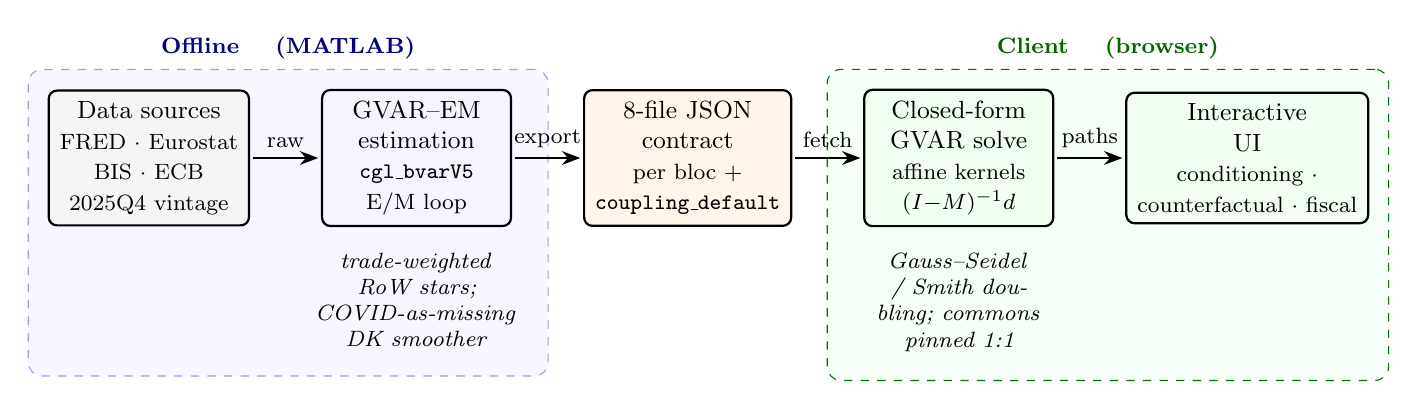
\begin{tikzpicture}[
  font=\small,
  >=Stealth,
  node distance=9mm,
  stage/.style={
    rounded corners=3pt, draw, thick, align=center,
    minimum height=15mm, minimum width=24mm, inner sep=4pt,
    fill=blue!4
  },
  data/.style={stage, fill=gray!8},
  contract/.style={stage, fill=orange!8},
  client/.style={stage, fill=green!6},
  flow/.style={->, thick, shorten >=1pt, shorten <=1pt},
  bandlbl/.style={font=\footnotesize\itshape}
]

% ---- stages, left to right ----
\node[data] (src) {Data sources\\\footnotesize FRED $\cdot$ Eurostat\\\footnotesize BIS $\cdot$ ECB\\\footnotesize 2025Q4 vintage};
\node[stage, right=of src] (est) {GVAR--EM\\estimation\\\footnotesize \texttt{cgl\_bvarV5}\\\footnotesize E/M loop};
\node[contract, right=of est] (json) {8-file JSON\\contract\\\footnotesize per bloc $+$\\\footnotesize \texttt{coupling\_default}};
\node[client, right=of json] (solve) {Closed-form\\GVAR solve\\\footnotesize affine kernels\\\footnotesize $(I{-}M)^{-1}d$};
\node[client, right=of solve] (ui) {Interactive\\UI\\\footnotesize conditioning $\cdot$\\\footnotesize counterfactual $\cdot$ fiscal};

% ---- flow arrows with labels ----
\draw[flow] (src) -- node[above, font=\footnotesize] {raw} (est);
\draw[flow] (est) -- node[above, font=\footnotesize] {export} (json);
\draw[flow] (json) -- node[above, font=\footnotesize] {fetch} (solve);
\draw[flow] (solve) -- node[above, font=\footnotesize] {paths} (ui);

% ---- under-arrows: methodological annotations ----
\node[below=2mm of est, bandlbl, text width=26mm, align=center] (estsub)
  {trade-weighted RoW stars; COVID-as-missing DK smoother};
\node[below=2mm of solve, bandlbl, text width=26mm, align=center] (solvesub)
  {Gauss--Seidel / Smith doubling; commons pinned 1:1};

% ---- background bands: offline (MATLAB) vs client (browser) ----
\begin{scope}[on background layer]
  \node[fit=(src)(est)(estsub), draw=blue!40, dashed, rounded corners=5pt,
        fill=blue!3, inner sep=7pt,
        label={[blue!55!black,font=\footnotesize\bfseries]above:Offline \quad (MATLAB)}] (offband) {};
  \node[fit=(solve)(ui)(solvesub), draw=green!45!black, dashed, rounded corners=5pt,
        fill=green!4, inner sep=7pt,
        label={[green!40!black,font=\footnotesize\bfseries]above:Client \quad (browser)}] (clband) {};
\end{scope}

\end{tikzpicture}%
}
\caption[End-to-end system architecture]{End-to-end system architecture of the EM-Bayesian Global VAR platform.
Harmonized macro-financial data (FRED, Eurostat, BIS, ECB; common 2025Q4 \emph{estimation} vintage, with
the observed panel subsequently refreshed to 2026Q1 with no re-estimation, \S\ref{sec:vintage}) feed the
\emph{offline} MATLAB GVAR--EM estimator: per-bloc Bayesian VARs (\texttt{cgl\_bvarV5}) are re-fit in an
EM loop that, at each sweep, rebuilds the trade-weighted rest-of-world ``star'' variables
(ROWDEM/ROWINF/ROWFIN) from partners' Durbin--Koopman-completed panels and re-estimates every bloc with
the 2020Q2--Q4 \emph{macro} columns masked (the foreign-rate star ROWFIN and all domestic financials kept
observed; COVID-as-missing), iterating to $\max|\Delta\text{star}|<0.03$ (cf.\ \S\ref{sec:gvar}). Each
converged bloc is serialized to the eight-file JSON contract (\texttt{spec}, \texttt{companion\_mean},
\texttt{companion\_draws}, \texttt{baseline}, \texttt{baseline\_levels}, \texttt{historical},
\texttt{historical\_levels}, \texttt{transformations}; plus \texttt{fiscal\_meta} and the precomputed
\texttt{coupling\_default.json.gz} coupling artifact). In the \emph{client} (browser), the cross-country
system is solved in closed form: the scenario delta obeys the affine fixed point $x = Mx + d$, evaluated by
Gauss--Seidel sweeps or directly via $(I-M)^{-1}d$ (Smith doubling), with global commons (US WTI oil,
US~10Y, US~BAA, US~equity) pinned 1:1 onto every RoW bloc. The interactive UI exposes conditioning,
counterfactuals, and the stock-flow fiscal block (\S\ref{sec:fiscal}).}
\label{fig:architecture}
\end{figure}
%% ================================================================

Conditional forecasting with Bayesian vector autoregressions (BVARs)
has become a standard tool in central bank forecasting and policy
analysis.  The seminal contributions of
\citet{DoanLittermanSims1984} and \citet{WaggonerZha1999}
established the methodological foundations, while
\citet{BanburaGiannoneLenza2015} extended these techniques to large
cross-sections using state-space methods.  The Monetary-Financial
Model described in this document builds on this literature to provide an
interactive, browser-based platform that makes conditional forecasting
and policy counterfactual analysis accessible without specialized
software.

The tool implements a three-layer analytical framework:
\begin{enumerate}[label=(\roman*)]
  \item \textbf{Baseline forecast:} An unconditional forecast from a
    large BVAR estimated on quarterly macroeconomic and financial data,
    following the hierarchical prior framework of \citet{Giannone2015}.
  \item \textbf{Conditional scenario:} The user conditions any subset
    of variables on desired paths; a Durbin--Koopman smoother
    \citep{DurbinKoopman2002, DurbinKoopman2012} propagates these
    constraints to all remaining variables, respecting the full
    covariance structure of the VAR.
  \item \textbf{Policy counterfactual:} An alternative monetary or
    fiscal policy path is overlaid on the scenario using impulse
    response functions from a DSGE model drawn from the Macroeconomic
    Model Data Base \citep[MMB;][]{WielandCwikMuellerSchmidtWolters2012},
    and the resulting macroeconomic responses are re-conditioned through
    the BVAR to ensure cross-variable consistency.
\end{enumerate}

The tool is designed for economists at central banks and international
institutions who need to construct and communicate conditional
projections and policy scenarios.  It runs entirely in the browser,
requiring no server-side computation, and can be deployed as a static
website on any hosting platform.

This document is organized as follows.  Section~\ref{sec:bvar}
describes the BVAR estimation methodology.
Section~\ref{sec:statespace} derives the companion-form state-space
representation.  Section~\ref{sec:kalman} presents the Kalman filter
and Durbin--Koopman smoother used for conditional forecasting.
Section~\ref{sec:counterfactual} details the policy counterfactual
framework.  Section~\ref{sec:variables} documents the variable
coverage.  Section~\ref{sec:interface} provides a guide to the user
interface.  Section~\ref{sec:technical} discusses technical
implementation details.  Section~\ref{sec:discussion} concludes with
a discussion of limitations and directions for future development.

\subsection{Notation}\label{sec:notation}

Table~\ref{tab:notation} collects the symbols used throughout the manual,
grouped by the layer in which they appear (BVAR estimation, the
companion-form state space and smoother, the GVAR coupling, the fiscal
recursion, and the long-run drift setter). A plain-language \emph{Glossary} of
the named concepts---BVAR, GVAR, the trade-weighted stars, COVID-as-missing, the
stock-flow adjustment, the EM loop, the endogenous dominant unit, the long-run
drift setter, and the evaluation statistics (CRPS, Giacomini--White, $\dots$)---is
provided in Appendix~\ref{app:glossary}.

\begin{small}
\begin{longtable}{@{}p{0.16\textwidth}p{0.78\textwidth}@{}}
\caption{Notation used across the BVAR, GVAR, fiscal, and long-run layers.}
\label{tab:notation}\\
\toprule
\textbf{Symbol} & \textbf{Meaning} \\
\midrule
\endfirsthead
\multicolumn{2}{@{}l}{\footnotesize\itshape Table~\ref{tab:notation} continued from previous page}\\
\toprule
\textbf{Symbol} & \textbf{Meaning} \\
\midrule
\endhead
\midrule
\multicolumn{2}{r@{}}{\footnotesize\itshape continued on next page}\\
\endfoot
\bottomrule
\endlastfoot
\multicolumn{2}{@{}l}{\textit{BVAR estimation (Sec.~\ref{sec:bvar})}}\\
$y_t$ & $n\times 1$ vector of endogenous variables of a bloc at quarter $t$ (in estimation space). \\
$n$ & number of variables in a bloc ($n=41$ for the endogenous-US bloc). \\
$p$ & VAR lag order ($p=3$ throughout). \\
$B_\ell$ & $n\times n$ reduced-form autoregressive coefficient matrix on lag $\ell$. \\
$\varepsilon_t$ & reduced-form innovation, $\varepsilon_t\sim\mathcal{N}(0,\Sigma)$. \\
$\Sigma$ & $n\times n$ innovation covariance; posterior-mean $\hat\Sigma$. \\
$\beta$, $\hat\beta$ & stacked VAR coefficients; posterior mean. \\
$\lambda$ & overall Minnesota/GLP shrinkage (tightness) hyperparameter. \\
$\mu$ & sum-of-coefficients prior hyperparameter \citep{Giannone2015}. \\
$\psi$ & residual-variance scale of the prior (per variable). \\
$\delta_i$ & prior mean on variable $i$'s own first lag: $\delta_i=1$ (random walk, \texttt{RW}) or $\delta_i=0$ (stationary white noise, \texttt{WN}). \\
$\texttt{pos}$ & index set of the \texttt{WN} variables; sets \(\texttt{diagb}(\texttt{pos})=0\) (Sec.~\ref{sec:ownlag}). \\
$D$ & number of retained posterior draws $\{(\hat\beta^{(d)},\hat\Sigma^{(d)})\}$. \\
\midrule
\multicolumn{2}{@{}l}{\textit{State space \& smoother (Sec.~\ref{sec:statespace}--\ref{sec:kalman})}}\\
$\alpha_t$ & companion-form state vector (stacked current and lagged $y$). \\
$T,Z,Q,H$ & transition, observation, state-noise, and measurement-noise matrices. \\
$Z_t^{(o)}$ & rows of $Z$ corresponding to the \emph{observed} variables at $t$ (partial observation). \\
$\alpha_{t|t-1},P_{t|t-1}$ & one-step predicted state mean and covariance. \\
$v_t,F_t,K_t$ & innovation, innovation variance, Kalman gain. \\
$r_t,L_t$ & Durbin--Koopman backward recursion vector and transition. \\
$\alpha_{t|H}$ & smoothed (full-interval) state. \\
$\mathcal{W}$ & COVID-as-missing window (the fixed three quarters 2020Q2--Q4). \\
\midrule
\multicolumn{2}{@{}l}{\textit{GVAR coupling (Sec.~\ref{sec:gvar})}}\\
$c,j$ & bloc (economy) indices; $c$ receiver, $j$ partner. \\
$w_{cj}$ & trade weight of partner $j$ in bloc $c$'s stars, $\sum_j w_{cj}=1$. \\
$\texttt{ROWDEM},\texttt{ROWINF},\texttt{ROWFIN}$ & trade-weighted foreign demand, inflation, and financial ``star'' variables. \\
$s_{c,v,t}$ & scenario pin-delta of bloc $c$'s star $v$ at horizon $t$. \\
$g\Delta_{p,t}$ & deviation of US-determined global column $p$ (oil, US10Y, USBAA, USeq). \\
$x$ & stacked deviation state of the coupling fixed point. \\
$M$ & solve-time coupling operator; $x=Mx+d$. \\
$d$ & exogenous forcing (own-scenario pins) of the fixed point. \\
$\rho(M)$ & spectral radius of $M$ (multiplier strength; $<1$ $\Rightarrow$ contractive). \\
\midrule
\multicolumn{2}{@{}l}{\textit{Fiscal recursion (Sec.~\ref{sec:fiscal})}}\\
$d_t$ & gross public debt as a percent of GDP. \\
$\mathit{rev}_t,\mathit{pexp}_t$ & revenue and primary expenditure (\% of GDP); \texttt{FREV\_GDP}, \texttt{FPEXP\_GDP}. \\
$i^{\text{eff}}_t$ & effective interest rate (\texttt{EFFI}, \% p.a.). \\
$\mathit{sfa}_t$ & stock-flow adjustment (\texttt{SFA}, \% of GDP). \\
$g^{n}_t$ & nominal GDP growth. \\
$\mathit{pb}_t$ & primary balance $=\mathit{rev}_t-\mathit{pexp}_t$. \\
\midrule
\multicolumn{2}{@{}l}{\textit{Long-run targets \& evaluation (Sec.~\ref{sec:longrun},~\ref{sec:empirical})}}\\
$\psi^\star_j,\psi^{\,0}_j$ & user long-run target and current terminal display forecast of variable $j$. \\
$c,\,\delta c_j$ & companion drift (constant row); shift of variable $j$'s own equation. \\
$S_h$ & partial companion-power sum $\sum_{k<h}T^{k}$; $S_h[:,j]\,\delta c_j$ is the response. \\
$\mathrm{sens}_j$ & display-unit sensitivity of $j$'s terminal forecast to a unit $\delta c_j$. \\
$h$ & forecast horizon (quarters); $h\in\{1,2,4,8\}$ in the horse-race. \\
$t_0$ & forecast origin in the recursive out-of-sample scheme. \\
$d_t$ (loss) & loss differential between two models at $t$ (overloads $d_t$; context disambiguates). \\
$\mathrm{CRPS}$ & continuous ranked probability score (primary density metric). \\
\end{longtable}
\end{small}

%% ================================================================
\section{BVAR Estimation}\label{sec:bvar}
%% ================================================================

\subsection{Reduced-Form VAR}

Consider an $n$-variable VAR($p$) in reduced form:
\begin{equation}\label{eq:var}
  y_t = c + \sum_{\ell=1}^{p} B_\ell\, y_{t-\ell} + u_t,
  \qquad u_t \sim \mathcal{N}(0, \Sigma),
\end{equation}
where $y_t \in \R^n$ is the vector of observables, $c \in \R^n$ is a
vector of intercepts, $B_1, \ldots, B_p \in \R^{n \times n}$ are the
autoregressive coefficient matrices, and $\Sigma \in \R^{n \times n}$
is the positive-definite innovation covariance matrix.  In the US
specification, $n = 41$ and $p = 3$, yielding a coefficient matrix
$\hat\beta \in \R^{124 \times 41}$ (with row~0 containing the
intercept).  The $41$ US variables include the four US-determined
\emph{global commons} (\texttt{GLB\_OIL}, \texttt{GLB\_USLR},
\texttt{GLB\_USBAA}, \texttt{GLB\_USEQ}) that the GVAR layer of
Section~\ref{sec:gvar} carries into every other bloc, the four-variable fiscal
block (Section~\ref{sec:fiscal}), and the three trade-weighted \texttt{ROW*\_US}
star variables through which the US, now an endogenous GVAR bloc, receives
Rest-of-World feedback.

\subsection{Data Transformations}

Variables enter the VAR in one of two forms:
\begin{itemize}
  \item \textbf{Log-transformed} ($\texttt{log}$): the variable is
    modeled in log levels.  Growth rates displayed to the user are
    quarter-over-quarter annualized:
    \begin{equation}\label{eq:growth}
      g_t^{\text{q/q ann.}} = 400 \times
      \bigl(\ln Y_t - \ln Y_{t-1}\bigr).
    \end{equation}
    Year-over-year growth rates are computed as:
    \begin{equation}\label{eq:yoy}
      g_t^{\text{y/y}} = 100 \times
      \bigl(\ln Y_t - \ln Y_{t-4}\bigr).
    \end{equation}
  \item \textbf{Linear} ($\texttt{lin}$): the variable enters in
    levels (e.g., interest rates in percent, unemployment rate).
    No growth-rate conversion is applied.
\end{itemize}

\subsection{Reporting Units}\label{sec:units}

The display unit is chosen per variable for interpretability, independently
of the estimation transformation:
\begin{itemize}
  \item \textbf{National-accounts / activity flows} (GDP, consumption,
    investment, trade volumes) are shown as growth (q/q annualized or y/y).
  \item \textbf{Prices} (CPI/HICP/deflators) are shown as inflation.
  \item \textbf{Rates and ratios} (policy and market rates, unemployment,
    fiscal ratios) are shown as levels in percent / percentage points.
    Unemployment-rate uncertainty bands are floored at~0 (a rate cannot be
    negative); policy and market rates are \emph{not} floored, because
    negative nominal rates do occur.
  \item \textbf{Index / FX / equity / commodity series} (the
    trade-weighted dollar \texttt{FXTWM}, US equity \texttt{GLB\_USEQ},
    house prices \texttt{HP}, oil \texttt{PZTEXP}/\texttt{GLB\_OIL}, the
    non-fuel commodity index
    \texttt{GSNE}, and the other blocs' \texttt{NEER\_EA},
    \texttt{NEER\_UK}, \texttt{NEER\_CA}, \texttt{REER\_CN},
    \texttt{EQ\_CN}) are reported as the \emph{index level}
    (e.g.\ 2010 $=100$) rather than as q/q growth: a trade-weighted
    exchange rate or equity index q/q-annualized is not an informative
    number, whereas its level is. These series remain \texttt{log} for
    estimation and are conditioned in the stored $100\ln(\text{index})$
    space; only the display is exponentiated back to the level,
    $\exp(\text{stored}/100)$, with a level-space uncertainty fan.
\end{itemize}

\subsection{Hierarchical Minnesota Prior}\label{sec:prior}

The model is estimated following \citet{Giannone2015}, who cast the
Minnesota prior \citep{Litterman1986, DoanLittermanSims1984} in a
hierarchical framework with data-driven hyperparameter selection.
The prior specification includes:
\begin{enumerate}[label=(\alph*)]
  \item The \textbf{Minnesota shrinkage} prior on $B_\ell$, centered
    on the random-walk or white-noise prior for each variable
    (depending on the variable's stationarity properties).  The
    tightness parameter $\lambda$ controls the overall degree of
    shrinkage toward the prior mean.
  \item The \textbf{sum-of-coefficients} prior
    \citep{DoanLittermanSims1984}, which shrinks toward the belief
    that a unit increase in every variable's level produces a unit
    increase in its forecast, imposing a form of cointegration.
  \item The \textbf{single-unit-root} prior, which constrains the
    system to have at most one common stochastic trend.
\end{enumerate}

The hyperparameters governing the tightness of each prior component
are treated as additional parameters and selected by maximizing the
marginal likelihood, as advocated by \citet{Giannone2015}.

Posterior draws are obtained via Markov chain Monte Carlo (MCMC).
The estimator runs a long chain with burn-in, retaining the posterior
mean $\hat\beta$ and $\hat\Sigma$ for the deterministic conditional
forecasting engine. For the browser the chain is \emph{thinned} to
$D=500$ retained draws
$\bigl\{(\hat\beta^{(d)}, \hat\Sigma^{(d)})\bigr\}_{d=1}^{D}$, the count
shipped in every bloc's \texttt{companion\_draws.json}, used for
uncertainty quantification via the simulation smoother
(Section~\ref{sec:uncertainty}). The thinned export keeps the per-bloc
draw artifact small enough to load on demand (the US file is
$\approx 34$\,MB at $D=500$, $n=41$, $p=3$).

\subsection{Per-variable own-lag prior mean: random walk vs.\ stationary}\label{sec:ownlag}

The Minnesota/GLP prior is centered, for each equation, on a univariate
model in which the variable's own first lag carries a prior mean of
$\delta_i$ and every other coefficient a prior mean of zero
\citep{Litterman1986,DoanLittermanSims1984,Giannone2015}. The
\emph{default} choice $\delta_i=1$ encodes a random-walk (\texttt{RW})
prior belief---``the best forecast of the level is the current level''---which
is appropriate for variables that are (near-)integrated in the
estimation space (log real activity, log price levels, nominal yields).
For a variable that is genuinely \emph{stationary}---a mean-reverting
ratio or rate that fluctuates around a constant level---the random-walk
center is the wrong null: it shrinks the dynamics toward a unit root and
lets the variable \emph{drift} at long horizons rather than return to its
historical mean. For such variables the tool sets the own-lag prior mean
to $\delta_i=0$, a stationary white-noise (\texttt{WN}) prior whose null
model is ``the best forecast is the unconditional mean (the equation
constant), not the last observation.''

\paragraph{The mechanism (\texttt{pos}/\texttt{stationary}).} The choice
is implemented exactly once, at the point where the prior mean of the
coefficient matrix is built. In
\texttt{BVAR/MFBVAR/GLPreplicationWeb/bvarGLPmf.m} the own-first-lag
prior block is the diagonal matrix \(\texttt{diag}(\texttt{diagb})\) with
\(\texttt{diagb}=\mathbf{1}_n\) by default; the line
\[
  \texttt{diagb}(\texttt{pos}) = 0
\]
zeroes the own-lag prior mean for every variable index in the vector
\texttt{pos}, so those equations are shrunk toward white noise instead of
a random walk. The index set is threaded into the sampler as the third
positional argument \texttt{stationary} of
\texttt{BVAR/MFBVAR/cgl\_bvarV5.m} (internally \(\texttt{pos} =
\texttt{stationary}\)), which forwards it as the \texttt{'pos'} option to
\texttt{bvarGLPmf}. The estimators build the set directly from the
per-variable \texttt{prior} tag in each bloc's specification,
\[
  \texttt{pos} \;=\; \texttt{find}(\texttt{prior}==\text{`}\texttt{WN}\text{'}),
\]
so a variable opts in to the stationary prior simply by carrying
\texttt{prior:"WN"} in its spec (see
\texttt{pipeline/export\_bvar\_gvar24\_loop.m} and
\texttt{pipeline/export\_bvar\_euro\_fsap.m}). For the $44$ non-fiscal
blocs the set is empty and the call is byte-identical to the historical
all-\texttt{RW} behaviour.

\paragraph{Prior, not constraint.} Crucially $\delta_i=0$ sets only the
prior \emph{mean}; it does not \emph{impose} stationarity. The posterior
own-lag coefficient is the usual GLP balance of prior and likelihood,
governed by the estimated tightness $\lambda$ (itself selected by the
marginal-likelihood maximization, Section~\ref{sec:prior}). A genuinely
persistent series whose data favour a near-unit root will still produce a
large posterior own-lag coefficient despite the white-noise center; the
\texttt{WN} prior simply removes the \emph{built-in} drift that the
random-walk center would otherwise inject at the long end. This is the
mechanism that makes the fiscal GDP-ratios mean-revert
(Section~\ref{sec:fiscal_drivers}).


%% ================================================================
\section{Companion-Form State Space}\label{sec:statespace}
%% ================================================================

To apply the Kalman filter, the VAR($p$) in~\eqref{eq:var} is cast in
companion form as a first-order state-space model
\citep[see, e.g.,][ch.~3]{DurbinKoopman2012}.

\subsection{State Vector}

Define the $np$-dimensional state vector:
\begin{equation}\label{eq:state}
  \alpha_t = \begin{pmatrix} y_t \\ y_{t-1} \\ \vdots \\ y_{t-p+1}
  \end{pmatrix} \in \R^{np}.
\end{equation}

\subsection{Transition Equation}

The state evolves according to:
\begin{equation}\label{eq:transition}
  \alpha_t = T\, \alpha_{t-1} + d + R\, \eta_t,
  \qquad \eta_t \sim \mathcal{N}(0, \Sigma),
\end{equation}
where the $np \times np$ transition matrix $T$, the $np$-dimensional
intercept vector $d$, and the $np \times n$ selection matrix $R$ are:
\begin{equation}\label{eq:companion}
  T = \begin{pmatrix}
    B_1' & B_2' & \cdots & B_{p-1}' & B_p' \\
    I_n  & 0    & \cdots & 0        & 0    \\
    0    & I_n  & \cdots & 0        & 0    \\
    \vdots & & \ddots & & \vdots \\
    0    & 0    & \cdots & I_n      & 0
  \end{pmatrix}, \quad
  d = \begin{pmatrix} c \\ 0 \\ \vdots \\ 0 \end{pmatrix}, \quad
  R = \begin{pmatrix} I_n \\ 0 \\ \vdots \\ 0 \end{pmatrix}.
\end{equation}

\begin{remark}
The $B_\ell'$ blocks in $T$ are transposed relative to \eqref{eq:var}
because the coefficient matrix $\hat\beta$ is stored as
$(1 + np) \times n$, with row~0 containing the intercept $c$ and
rows $1, \ldots, np$ containing the stacked lag coefficients.
Specifically, $T(i,j) = \hat\beta(j+1, i)$ for $0 \le i < n$ and
$0 \le j < np$.
\end{remark}

\subsection{Observation Equation}

The observation equation extracts the contemporaneous variables:
\begin{equation}\label{eq:obs}
  y_t = Z\, \alpha_t + \varepsilon_t,
  \qquad \varepsilon_t \sim \mathcal{N}(0, H),
\end{equation}
where $Z = \bigl(I_n \mid 0_{n \times n(p-1)}\bigr)$ and
$H = \sigma^2_\varepsilon I_n$ with $\sigma^2_\varepsilon = 10^{-12}$
(a negligible measurement error included for numerical stability of the
Kalman filter recursions).

\subsection{State-Noise Covariance}

The $np \times np$ state-noise covariance matrix is:
\begin{equation}\label{eq:Q}
  Q = R\, \Sigma\, R' = \begin{pmatrix}
    \Sigma & 0 & \cdots & 0 \\
    0      & 0 & \cdots & 0 \\
    \vdots & & \ddots & \\
    0      & 0 & \cdots & 0
  \end{pmatrix}.
\end{equation}


%% ================================================================
\section{Kalman Filter and Smoother}\label{sec:kalman}
%% ================================================================

\subsection{Conditioning via Partial Observations}\label{sec:partial}

The key insight underlying conditional forecasting in a state-space
framework, following \citet{BanburaGiannoneLenza2015}, is that
conditioning on variable~$i$ at horizon~$h$ is equivalent to observing
$y_{T+h,i}$ in the Kalman filter.  For each forecast period
$t = T+1, \ldots, T+H$, the observation vector is partitioned into:
\begin{itemize}
  \item \textbf{Conditioned variables:} $y_t^{(o)}$, with known
    target values specified by the user.
  \item \textbf{Free variables:} $y_t^{(m)}$, treated as missing
    observations (coded as \texttt{NaN}).
\end{itemize}
The Kalman filter processes only the observed subset at each time
step, adapting $Z_t$, $H_t$, and the innovation $v_t$ accordingly.

\subsection{Forward Pass: Kalman Filter}\label{sec:kf}

\paragraph{Algorithm: Kalman Filter with Partial Observations.}
\label{alg:kf}
\textbf{Input:} $T, Z, Q, H, d$; initial state $\alpha_0$,
covariance $P_0$; partial observations $\{y_t^{(o)}\}_{t=1}^{H}$.

\noindent For $t = 1, \ldots, H$:
\begin{align}
  \alpha_{t|t-1} &= T\, \alpha_{t-1|t-1} + d
    & &\text{(state prediction)} \label{eq:kf_pred_a} \\
  P_{t|t-1} &= T\, P_{t-1|t-1}\, T' + Q
    & &\text{(covariance prediction)} \label{eq:kf_pred_P}
\end{align}
If observations exist at time $t$, let $Z_t^{(o)}$ be the rows of $Z$
for observed variables, then:
\begin{align}
  v_t &= y_t^{(o)} - Z_t^{(o)}\, \alpha_{t|t-1}
    & &\text{(innovation)} \label{eq:kf_innov} \\
  F_t &= Z_t^{(o)}\, P_{t|t-1}\, (Z_t^{(o)})' + H_t^{(o)}
    & &\text{(innovation variance)} \label{eq:kf_F} \\
  K_t &= P_{t|t-1}\, (Z_t^{(o)})'\, F_t^{-1}
    & &\text{(Kalman gain)} \label{eq:kf_K} \\
  \alpha_{t|t} &= \alpha_{t|t-1} + K_t\, v_t
    & &\text{(state update)} \label{eq:kf_upd_a} \\
  P_{t|t} &= P_{t|t-1} - K_t\, Z_t^{(o)}\, P_{t|t-1}
    & &\text{(covariance update)} \label{eq:kf_upd_P}
\end{align}
If no observations exist at time $t$: $\alpha_{t|t} = \alpha_{t|t-1}$
and $P_{t|t} = P_{t|t-1}$.

The matrix inversion $F_t^{-1}$ is computed via LU decomposition with
partial pivoting; singularity is flagged when the pivot falls below
$10^{-15}$.

\subsection{Backward Pass: Durbin--Koopman Smoother}\label{sec:dk}

\begin{figure}[!ht]
\centering
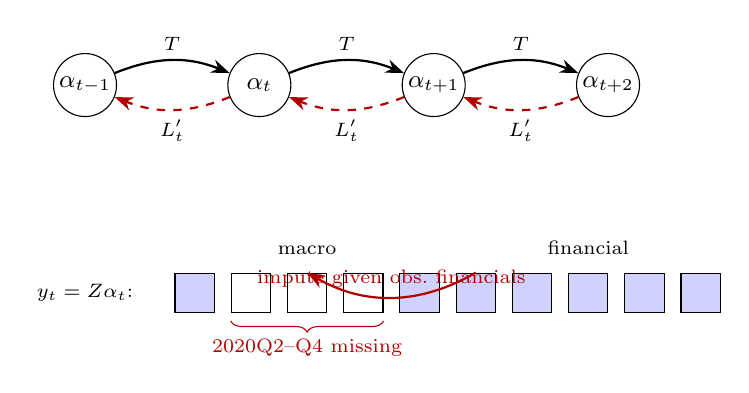
\begin{tikzpicture}[
    >=Stealth,
    font=\small,
    state/.style={circle,draw,minimum size=8mm,inner sep=0pt},
    obsfill/.style={rectangle,draw,minimum size=5mm,inner sep=0pt,fill=blue!18},
    obshollow/.style={rectangle,draw,minimum size=5mm,inner sep=0pt,fill=white},
    filt/.style={->,draw=black,thick},
    smth/.style={->,draw=red!70!black,thick,dashed},
    node distance=14mm,
]
% ---- state timeline ----
\node[state] (a1) {$\alpha_{t-1}$};
\node[state,right=of a1] (a2) {$\alpha_{t}$};
\node[state,right=of a2] (a3) {$\alpha_{t+1}$};
\node[state,right=of a3] (a4) {$\alpha_{t+2}$};

% forward Kalman filter (transition T) above
\draw[filt] (a1) to[bend left=22] node[above,font=\scriptsize]{$T$} (a2);
\draw[filt] (a2) to[bend left=22] node[above,font=\scriptsize]{$T$} (a3);
\draw[filt] (a3) to[bend left=22] node[above,font=\scriptsize]{$T$} (a4);

% backward DK smoother below
\draw[smth] (a4) to[bend left=22] node[below,font=\scriptsize]{$L_{t}'$} (a3);
\draw[smth] (a3) to[bend left=22] node[below,font=\scriptsize]{$L_{t}'$} (a2);
\draw[smth] (a2) to[bend left=22] node[below,font=\scriptsize]{$L_{t}'$} (a1);

% ---- observation row (COVID window 2020Q2--Q4) ----
\node[below=20mm of a1,anchor=north] (lab) {\scriptsize $y_t = Z\alpha_t$:};
% macro cells (hollow over the 3 COVID quarters)
\node[obsfill,right=4mm of lab] (m1) {};
\node[obshollow,right=2mm of m1] (m2) {};
\node[obshollow,right=2mm of m2] (m3) {};
\node[obshollow,right=2mm of m3] (m4) {};
\node[obsfill,right=2mm of m4]  (m5) {};
% financial cells (filled throughout)
\node[obsfill,right=2mm of m5] (f1) {};
\node[obsfill,right=2mm of f1] (f2) {};
\node[obsfill,right=2mm of f2] (f3) {};
\node[obsfill,right=2mm of f3] (f4) {};
\node[obsfill,right=2mm of f4] (f5) {};

\node[above=1mm of m3,font=\scriptsize] {macro};
\node[above=1mm of f3,font=\scriptsize] {financial};
% COVID bracket under the 3 missing macro cells
\draw[decorate,decoration={brace,amplitude=4pt,mirror},red!70!black]
   ($(m2.south west)+(0,-1mm)$) -- ($(m4.south east)+(0,-1mm)$)
   node[midway,below=3pt,font=\scriptsize,red!70!black]{2020Q2--Q4 missing};

% imputation arrow: observed financials -> imputed (hollow) macro hole
\draw[->,red!70!black,thick] (f1.north) to[bend left=30]
   node[above,font=\scriptsize]{impute given obs.\ financials} (m3.north);
\end{tikzpicture}
\caption{Companion-form state space with the Durbin--Koopman
filter/smoother under the COVID-as-missing treatment.  States
$\alpha_t$ (Eq.~\eqref{eq:state}) evolve forward through the transition
matrix $T$ (solid, Kalman filter, Eq.~\eqref{eq:kf_pred_a}); the
backward smoother propagates
$r_{t-1}=(Z_t^{(o)})'F_t^{-1}v_t+L_t'r_t$
(dashed, Eq.~\eqref{eq:dk_r}).  In the observation row
$y_t=Z\alpha_t$ (Eq.~\eqref{eq:obs}), over the fixed window
2020Q2--Q4 (three quarters) the \emph{macro} cells (real activity,
prices, and the macro stars ROWDEM/ROWINF) are set missing (hollow)
while the \emph{financial} cells (rates, yields, equity, house prices,
and the foreign-rate star ROWFIN) remain observed (filled).  Because
the filter processes only the observed rows $Z_t^{(o)}$ of each
partially-observed vector, the macro holes are imputed conditional on
the observed financials.}
\label{fig:statespace-dk}
\end{figure}

The smoother refines the filtered estimates using all future
information, yielding $\alpha_{t|H}$ for all~$t$
\citep{DurbinKoopman2002, DurbinKoopman2012}.

\paragraph{Algorithm: Durbin--Koopman Fixed-Interval Smoother.}
\label{alg:dk}
\textbf{Input:} Filtered quantities
$\{\alpha_{t|t-1}, P_{t|t-1}, v_t, Z_t^{(o)}, F_t\}_{t=1}^{H}$.

\noindent Initialize $r_H = 0$.  For $t = H, H{-}1, \ldots, 1$:

If observations exist at time $t$:
\begin{align}
  L_t &= T'\,\bigl(I - P_{t|t-1}\, (Z_t^{(o)})'\,
    F_t^{-1}\, Z_t^{(o)}\bigr), \label{eq:dk_L} \\
  r_{t-1} &= (Z_t^{(o)})'\, F_t^{-1}\, v_t + L_t'\, r_t.
    \label{eq:dk_r}
\end{align}
Otherwise: $r_{t-1} = T'\, r_t$.

\noindent The smoothed state is:
\begin{equation}\label{eq:dk_smooth}
  \alpha_{t|H} = \alpha_{t|t-1} + P_{t|t-1}\, r_{t-1}.
\end{equation}

\paragraph{Simulation smoother (draws, not just means).} For
uncertainty quantification and for the COVID-as-missing data
augmentation (Section~\ref{sec:covid}) the tool needs \emph{draws} of the
missing/conditioned states, not only their smoothed mean. The
\citet{DurbinKoopman2002} simulation smoother obtains a draw
$\tilde\alpha$ from the conditional distribution
$p(\alpha\mid y^{(o)})$ by the elegant ``mean-correction'' device:
simulate an unconditional path, smooth it, and add the smoothed
\emph{discrepancy} back to the unconditional draw. Algorithm
\ref{alg:dksmoother} states the form used inside each
\texttt{cgl\_bvarV5} sweep, with partial (ragged + COVID-masked)
observations handled by processing only the observed rows
$Z_t^{(o)}$ at each date.

\begin{algorithm}[!ht]
\caption{Durbin--Koopman simulation smoother with partial observations
(one draw inside the data-augmentation Gibbs sweep).}
\label{alg:dksmoother}
\algIn{system matrices $T,Z,Q,H$; partial observations
$\{y_t^{(o)}\}_{t=1}^{H}$ (COVID-macro and ragged rows absent);
current draw of $(\beta,\Sigma)$.}
\algOut{one draw $\tilde\alpha_{1:H}$ from $p(\alpha_{1:H}\mid y^{(o)},\beta,\Sigma)$, hence imputed values for the missing $y$ cells.}
\begin{algsteps}
\item \algComment{(1) Forward simulation of an unconditional path.}
\item Draw $\alpha_0^{+}$ from the initial state law; \algKw{for} $t=1,\dots,H$: draw $\eta_t,\varepsilon_t$ and set $\alpha_t^{+}=T\alpha_{t-1}^{+}+\eta_t$, $\,y_t^{+}=Z\alpha_t^{+}+\varepsilon_t$.
\item Form the synthetic partial observations $y_t^{+(o)}$ on the \emph{same} observed pattern as the data ($\;$drop the cells that are \texttt{NaN} in $y_t^{(o)}$).
\item \algComment{(2) Kalman filter (Algorithm of Sec.~\ref{sec:kf}) on the artificial series $y_t^{(o)}-y_t^{+(o)}$.}
\item \algKw{for} $t=1,\dots,H$: run the prediction/update recursions on $Z_t^{(o)}$, storing $\{\alpha_{t|t-1},P_{t|t-1},v_t,F_t\}$. \algComment{at fully-missing $t$, no update}
\item \algComment{(3) Backward Durbin--Koopman smoothing recursion.}
\item Set $r_H=0$; \algKw{for} $t=H,\dots,1$:
\item \algInd \algKw{if} observed at $t$: $L_t = T'\bigl(I - P_{t|t-1}(Z_t^{(o)})'F_t^{-1}Z_t^{(o)}\bigr)$, $\;r_{t-1}=(Z_t^{(o)})'F_t^{-1}v_t + L_t'r_t$;
\item \algInd \algKw{else}: $r_{t-1}=T'r_t$.
\item \algInd smoothed discrepancy $\hat\alpha_t = \alpha_{t|t-1}+P_{t|t-1}r_{t-1}$.
\item \algComment{(4) Mean-correction: add the discrepancy back to the unconditional draw.}
\item $\tilde\alpha_t \gets \alpha_t^{+} + \hat\alpha_t$; read the imputed $\tilde y_t = Z\tilde\alpha_t$ at the missing cells.
\end{algsteps}
\end{algorithm}

Averaging $\tilde\alpha$ across Gibbs sweeps recovers the posterior-mean
completed panel $\widehat X_c$ that Algorithm~\ref{alg:emgvar} feeds back
into the stars; retaining the per-draw paths yields the predictive draw
cloud \texttt{Dforecast} used for the uncertainty bands
(Section~\ref{sec:bands}) and for density scoring
(Section~\ref{sec:empirical:oos}).

\subsection{Conditional Forecast Computation}

The conditional forecast is computed as follows:
\begin{enumerate}
  \item Initialize the state from the last $p$ historical
    observations: $\alpha_0 = (y_T', y_{T-1}', \ldots, y_{T-p+1}')'$.
  \item Construct the conditioning matrix $Y^* \in \R^{H \times n}$,
    where $Y^*_{t,j}$ is the target value for variable~$j$ at
    horizon~$t$ if conditioned, and $\texttt{NaN}$ otherwise.
  \item Run the Kalman filter (Algorithm~\ref{alg:kf}) and smoother
    (Algorithm~\ref{alg:dk}) with partial observations given
    by the non-$\texttt{NaN}$ entries of~$Y^*$.
  \item Extract the observation block (first $n$ elements) from each
    smoothed state $\alpha_{t|H}$.
\end{enumerate}

\subsection{Delta-Based Display}\label{sec:delta}

To ensure that zero user deviations produce exactly the stored
baseline forecast, the tool computes both an unconditional smoother
pass (with all entries of $Y^*$ set to $\texttt{NaN}$) and a
conditional pass.  The displayed forecast is:
\begin{equation}\label{eq:delta}
  \hat{y}_{T+h}^{\text{display}} = \bar{y}_{T+h}^{\text{baseline}}
  + \underbrace{\bigl(\hat{y}_{T+h}^{\text{cond}} -
  \hat{y}_{T+h}^{\text{uncond}}\bigr)}_{\text{smoother delta}},
\end{equation}
where $\bar{y}^{\text{baseline}}$ is the pre-computed baseline
forecast (posterior mean).  This construction guarantees that the
displayed forecast matches the stored baseline exactly when no
conditioning constraints are imposed, avoiding small numerical
discrepancies between the smoother's unconditional output and the
stored baseline.  The unconditional smoother result is cached and
reused across conditioning changes.

For log-transformed variables, the smoother operates in log-level
space, and the delta is scaled to annualized growth-rate space:
\begin{equation}\label{eq:scale}
  \Delta g_h = 4 \times \Delta \ell_h, \qquad
  \Delta \ell_h = \ell_h^{\text{cond}} - \ell_h^{\text{uncond}},
\end{equation}
where $\ell_h$ denotes the log-level forecast at horizon~$h$.

\subsection{Uncertainty Quantification}\label{sec:uncertainty}

Forecast uncertainty bands are computed via the Durbin--Koopman
\emph{simulation smoother} \citep{DurbinKoopman2002}, which generates
draws from the posterior predictive distribution conditional on the
user's constraints.

For each posterior draw $d = 1, \ldots, D$:
\begin{enumerate}
  \item \textbf{Forward simulation:} Draw shocks
    $\eta_t^+ \sim \mathcal{N}(0, I_n)$ and compute a simulated path
    using the $d$-th posterior draw of the VAR coefficients:
    \begin{equation}\label{eq:sim_forward}
      \alpha_{t}^+ = T^{(d)}\, \alpha_{t-1}^+ + d^{(d)}
      + R\, L^{(d)}\,\eta_t^+,
    \end{equation}
    where $L^{(d)}$ is the lower Cholesky factor of $\Sigma^{(d)}$.
    The simulated observations are $y_t^+ = Z\, \alpha_t^+$.
  \item \textbf{Deviation computation:} At conditioned entries,
    compute $y_t^* = Y_t^{\text{target}} - y_t^+$; at free entries,
    set $y_t^* = \texttt{NaN}$.
  \item \textbf{Smoother on deviations:} Run the Kalman smoother
    on $\{y_t^*\}$ with initial state $\alpha_0^* = 0$ and small
    initial covariance $P_0^* = 10^{-7} I_{np}$, producing
    adjustment paths $\hat\alpha_t^*$.
  \item \textbf{Combine:} The conditional draw is
    $\tilde\alpha_t = \hat\alpha_t^* + \alpha_t^+$.
\end{enumerate}
The 16th and 84th percentiles across $D$ draws yield the reported
68\% credible bands.  The tool uses $D = 50$ in ``Quick'' mode
and $D = 200$ in ``Full'' mode.  The simulation smoother correctly
integrates over both parameter uncertainty (through the posterior
draws) and forecast uncertainty (through the simulated shocks).


%% ================================================================
\section{Policy Counterfactuals}\label{sec:counterfactual}
%% ================================================================

The counterfactual layer evaluates how macroeconomic outcomes change
under an alternative policy stance.  It operates \emph{on top of} the
conditional scenario described in Section~\ref{sec:kalman}: starting
from the DK-smoothed scenario paths, the user specifies deviations in
the policy rate or government spending, and the tool traces the
implied effects through a DSGE model's impulse response functions
before re-conditioning the full system through the BVAR.

\subsection{DSGE Impulse Response Functions}\label{sec:dsge}

Impulse response functions (IRFs) are drawn from the Macroeconomic
Model Data Base \citep[MMB;][]{WielandCwikMuellerSchmidtWolters2012,
WielandAfanasyevaYooKuete2016}.  The MMB provides a library of
pre-solved DSGE models with standardized variable names and multiple
policy rule specifications.  The tool includes IRFs from 169~models
under 9~monetary policy rules:

\begin{center}
\begin{tabular}{ll}
\toprule
\textbf{Rule} & \textbf{Reference} \\
\midrule
Taylor      & \citet{Taylor1993} \\
SW          & \citet{SmetsWouters2007} \\
CEE         & \citet{CEE2005} \\
GR          & Gerdesmeier \& Roffia (2004) \\
LWW         & Levin, Wieland \& Williams (2003) \\
OW08        & Orphanides \& Wieland (2008) \\
OW13        & Orphanides \& Wieland (2013) \\
Coenen      & \citet{Coenen2012} \\
CMR         & Christiano, Motto \& Rostagno (2014) \\
\bottomrule
\end{tabular}
\end{center}

Each IRF file provides the dynamic response of key macroeconomic
variables---inflation, output gap, interest rate, consumption,
investment, and others---to a one-standard-deviation monetary policy
shock under the specified rule.  Fiscal policy IRFs are available for
60~models that include a fiscal sector.

\subsection{Monetary Policy Shock Inversion}\label{sec:shock_inversion}

Given a user-specified interest-rate adjustment path
$\Delta r = (\Delta r_1, \ldots, \Delta r_H)'$, the tool solves for
the structural monetary policy shock sequence
$\varepsilon = (\varepsilon_1, \ldots, \varepsilon_H)'$ via the
lower-triangular Toeplitz system:
\begin{equation}\label{eq:toeplitz}
  \underbrace{\begin{pmatrix}
    h_r(0) & 0 & \cdots & 0 \\
    h_r(1) & h_r(0) & \cdots & 0 \\
    \vdots & & \ddots & \vdots \\
    h_r(H{-}1) & h_r(H{-}2) & \cdots & h_r(0)
  \end{pmatrix}}_{\mathcal{H}_r \in \R^{H \times H}}
  \varepsilon = \Delta r,
\end{equation}
where $h_r(s)$ is the impulse response of the interest rate at
horizon~$s$.  Since $\mathcal{H}_r$ is lower-triangular, the system is
solved by forward substitution:
\begin{equation}\label{eq:shock_inversion_formula}
  \varepsilon_t = \frac{\Delta r_t - \sum_{j=0}^{t-1}
    h_r(t-j)\, \varepsilon_j}{h_r(0)}, \qquad t = 0, 1, \ldots, H{-}1.
\end{equation}

The implied responses of inflation and output are:
\begin{equation}\label{eq:irf_delta}
  \Delta \pi_t^{\text{IRF}} = \sum_{j=0}^{t} h_\pi(t{-}j)\,
  \varepsilon_j,
  \qquad
  \Delta y_t^{\text{IRF}} = \sum_{j=0}^{t} h_y(t{-}j)\,
  \varepsilon_j.
\end{equation}

An analogous procedure applies to fiscal policy shocks, using the
government-spending IRFs ($h_g$, $h_\pi^g$, $h_y^g$, $h_r^g$) from
the DSGE models in the MMB that include a fiscal sector.

\subsection{Three Conditioning Modes}\label{sec:modes}

After computing the DSGE-implied deltas, the counterfactual is
re-conditioned through the BVAR to enforce cross-variable
consistency.  Three modes govern what is held fixed versus free in
the second-stage DK smoother pass:

\begin{enumerate}[label=\textbf{(\alph*)}]
  \item \textbf{Hold-targets:} All user-conditioned variables are
    pinned at their scenario values; the interest rate is pinned at
    the scenario rate plus the adjustment.  Remaining variables are
    free and determined by the DK smoother:
    \begin{align}
      Y_t^{\text{cf}}(j) &= \hat{y}_{T+t,j}^{\text{cond}},
        & &\text{for } j \in \mathcal{C}, \\
      Y_t^{\text{cf}}(r) &= \hat{y}_{T+t,r}^{\text{cond}}
        + \Delta r_t, \\
      Y_t^{\text{cf}}(j) &= \texttt{NaN},
        & &\text{otherwise}.
    \end{align}

  \item \textbf{Let-adjust:} Only the policy instrument(s) are
    conditioned; all other variables, including inflation and output,
    are free and adjust endogenously through the BVAR covariance
    structure.

  \item \textbf{IRF-consistent} (default):  The interest rate is
    pinned at the scenario rate plus the adjustment, and inflation
    and output are pinned at the scenario values plus the
    DSGE-implied deltas from~\eqref{eq:irf_delta}:
    \begin{align}\label{eq:irf_consist}
      Y_t^{\text{cf}}(\pi) &= \hat{y}_{T+t,\pi}^{\text{cond}}
        + \Delta \pi_t^{\text{IRF}}, \\
      Y_t^{\text{cf}}(y) &= \hat{y}_{T+t,y}^{\text{cond}}
        + \Delta y_t^{\text{IRF}}, \\
      Y_t^{\text{cf}}(r) &= \hat{y}_{T+t,r}^{\text{cond}}
        + \Delta r_t.
    \end{align}
    The remaining variables are determined by the DK smoother,
    producing responses consistent with both the DSGE-identified
    monetary transmission and the BVAR covariance structure.
\end{enumerate}

In all modes, the counterfactual display uses the same delta
construction as~\eqref{eq:delta}:
\begin{equation}\label{eq:cf_display}
  \hat{y}_{T+h}^{\text{cf,display}} =
  \hat{y}_{T+h}^{\text{scen,display}}
  + f\!\bigl(\hat{y}_{T+h}^{\text{cf,smooth}}
  - \hat{y}_{T+h}^{\text{scen,smooth}}\bigr),
\end{equation}
where $f(\cdot)$ applies the $\times 4$ scaling from~\eqref{eq:scale}
for log-transformed variables.

\subsection{Optimal Policy: Barnichon--Mesters}\label{sec:bm}

Following \citet{BarnichonMesters2023}, the tool solves for the
optimal monetary policy shock sequence that minimizes a quadratic loss
function over deviations from target:
\begin{equation}\label{eq:loss}
  \mathcal{L} = \sum_{t=1}^{H} \Bigl[
    \lambda_\pi \bigl(\pi_t - \pi^*\bigr)^2
    + \lambda_y \bigl(y_t - y^*\bigr)^2
  \Bigr],
\end{equation}
subject to the linear mapping from shocks to outcomes given by the
DSGE impulse responses.

Define the Toeplitz matrices
$\mathcal{H}_\pi, \mathcal{H}_y \in \R^{H \times H}$ analogously
to~\eqref{eq:toeplitz} using the inflation and output-gap IRFs.
Stacking the weighted system:
\begin{equation}\label{eq:bm_stack}
  \underbrace{\begin{pmatrix}
    \sqrt{\lambda_\pi}\, \mathcal{H}_\pi \\[3pt]
    \sqrt{\lambda_y}\, \mathcal{H}_y
  \end{pmatrix}}_{\tilde{\mathcal{H}} \in \R^{2H \times H}}
  \varepsilon
  = \underbrace{\begin{pmatrix}
    \sqrt{\lambda_\pi}\, \Delta\pi^{\text{target}} \\[3pt]
    \sqrt{\lambda_y}\, \Delta y^{\text{target}}
  \end{pmatrix}}_{\tilde{b} \in \R^{2H}},
\end{equation}
the optimal shock sequence is obtained via Tikhonov-regularized
least squares:
\begin{equation}\label{eq:bm_solve}
  \varepsilon^* = \bigl(\tilde{\mathcal{H}}'\tilde{\mathcal{H}}
  + \alpha I_H\bigr)^{-1} \tilde{\mathcal{H}}'\, \tilde{b},
\end{equation}
with regularization parameter $\alpha = 10^{-6}$.  The implied policy
rate path is
$\Delta r_t^* = \sum_{j=0}^{t} h_r(t{-}j)\,\varepsilon_j^*$, which
is then passed to the IRF-consistent conditioning mode
(Section~\ref{sec:modes}c) to obtain the full counterfactual.

The user controls the relative weight on price stability versus full
employment via a slider that sets
$\lambda_\pi / (\lambda_\pi + \lambda_y)$.


%% ================================================================
\section{Global VAR (GVAR) and Global Commons}\label{sec:gvar}

The single-country engine of Sections~\ref{sec:bvar}--\ref{sec:counterfactual}
generalizes to a multi-country setting in which a conditioning imposed on one
economy spills over to all others. The tool implements a \emph{Global VAR}
(GVAR) layer in the tradition of \citet{PesaranSchuermannWeiner2004} and
\citet{DeesDiMauroPesaranSmith2007}, comprising the United States together with
the euro area as a single aggregate bloc and $31$ further Rest-of-World (RoW)
blocs---$33$ coupled blocs in all---that span approximately 90\% of global GDP.
The decisive implementation choice is that \emph{cross-country coupling is
imposed at solve time, not at estimation time}: each bloc is an independently
estimated single-country BVAR, and the spillovers enter only through the scenario
\emph{deviation}, which propagates as a linear fixed point. Two further channels
distinguish the current version: the United States is now a \emph{fully
endogenous} coupled bloc---it drives the rest of the world \emph{and} receives
feedback from it, rather than acting as a frozen anchor---and four US-determined
\emph{global commons} (oil, the long US rate, US corporate credit, and US equity)
are carried by every bloc.

\subsection{Architecture: an endogenous US and 32 partner blocs}\label{sec:gvar:arch}

\begin{figure}[!ht]
\centering
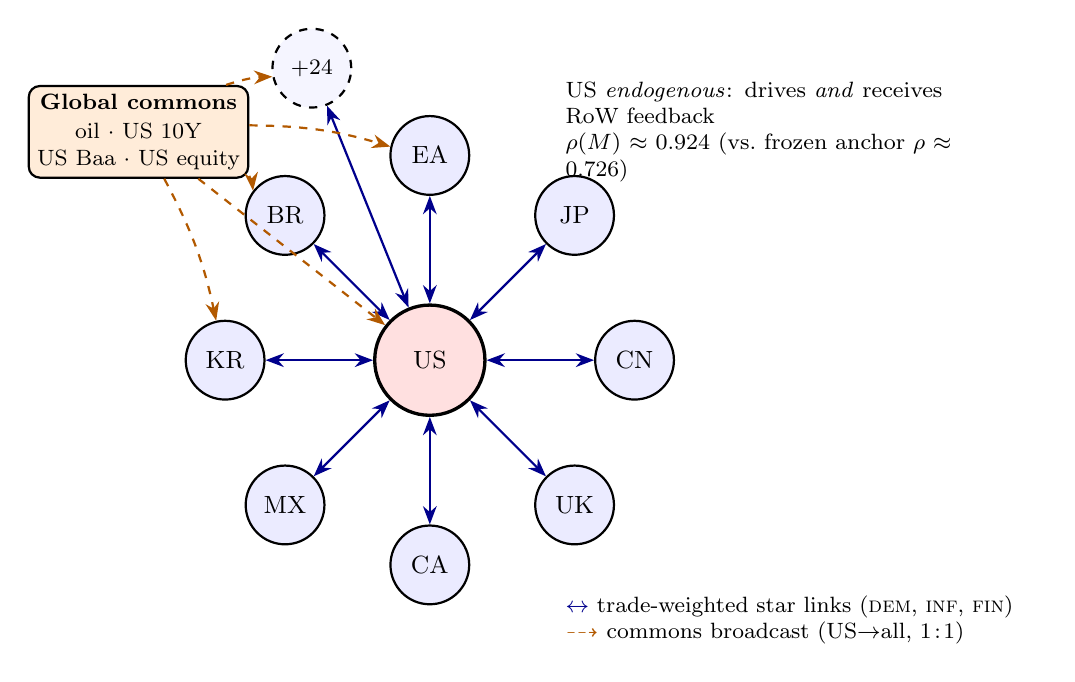
\begin{tikzpicture}[
  >=Stealth,
  font=\small,
  bloc/.style={circle, draw, thick, minimum size=10mm, inner sep=1pt, fill=blue!8},
  hub/.style={circle, draw, very thick, minimum size=14mm, inner sep=1pt, fill=red!12},
  commons/.style={rectangle, rounded corners, draw, thick, fill=orange!15,
                  align=center, inner sep=3pt, font=\footnotesize},
  star/.style={<->, thick, blue!55!black},
  bcast/.style={->, thick, orange!70!black, dashed},
]

% Central dominant US bloc (endogenous)
\node[hub] (US) at (0,0) {US};

% Ring of representative partner blocs (label ~8, indicate "+ 24 more")
\node[bloc] (EA)   at ( 90:2.6) {EA};
\node[bloc] (JP)   at ( 45:2.6) {JP};
\node[bloc] (CN)   at (  0:2.6) {CN};
\node[bloc] (UK)   at (-45:2.6) {UK};
\node[bloc] (CA)   at (-90:2.6) {CA};
\node[bloc] (MX)   at (-135:2.6) {MX};
\node[bloc] (KR)   at (180:2.6) {KR};
\node[bloc] (BR)   at (135:2.6) {BR};

% "+ 24 more" partner blocs
\node[bloc, fill=blue!4, dashed] (more) at (112:4.0) {\footnotesize $+24$};

% Bidirectional trade-weighted star links (US <-> each partner)
\foreach \c in {EA,JP,CN,UK,CA,MX,KR,BR} {\draw[star] (US) -- (\c);}
\draw[star] (US) -- (more);

% Global commons node broadcasting one-directionally to all blocs
\node[commons] (GC) at (-3.7,2.9)
  {\textbf{Global commons}\\[1pt]
   oil $\cdot$ US 10Y\\ US Baa $\cdot$ US equity};
\draw[bcast] (GC) -- (US);
\foreach \c in {EA,BR,KR,more} {\draw[bcast] (GC) to[bend left=8] (\c);}

% Legend / annotations
\node[align=left, font=\footnotesize, anchor=west, text width=6.0cm] at (1.6,-3.3)
  {\textcolor{blue!55!black}{$\leftrightarrow$}\ trade-weighted star links
     (\textsc{dem}, \textsc{inf}, \textsc{fin})\\
   \textcolor{orange!70!black}{$\dashrightarrow$}\ commons broadcast (US$\to$all, $1\!:\!1$)};
\node[align=left, font=\footnotesize, anchor=west, text width=5.4cm] at (1.6,2.9)
  {US \emph{endogenous}: drives \emph{and} receives RoW feedback\\
   $\rho(M)\!\approx\!0.924$ (vs.\ frozen anchor $\rho\!\approx\!0.726$)};

\end{tikzpicture}
\caption{GVAR bloc topology. A central, dominant United States bloc is coupled to
a ring of $32$ Rest-of-World partner blocs (eight labelled---EA, JP, UK, CA, CN,
MX, KR, BR---plus $24$ further blocs) through \emph{bidirectional},
trade-weighted ``RoW star'' links carrying foreign demand (\textsc{dem}),
inflation (\textsc{inf}), and the short rate (\textsc{fin}). A small global-commons
node (oil, the long US rate, US corporate credit, US equity) broadcasts
\emph{one-directionally} and identically ($1\!:\!1$) to every bloc. The US is now a
\emph{fully endogenous} coupled bloc rather than the classical frozen anchor: it
feeds the rest of the world \emph{and} receives feedback, raising the coupling
operator's spectral radius from $\rho(M)\approx0.726$ (frozen-US, RoW-only) to
$\rho(M)\approx0.924$ at the full $33$-bloc endogenous-US configuration (the value
stored in the shipped \texttt{coupling\_default.json.gz}; it moves slightly with
each refit), both contractive so the fixed point $x = Mx + d$ is well defined
(Sections~\ref{sec:gvar:arch}--\ref{sec:gvar:fixedpoint}).}
\label{fig:gvar-topology}
\end{figure}

The bloc set is
\texttt{US}, \texttt{EA}, \texttt{JP}, \texttt{UK}, \texttt{CA},
\texttt{CN}, \texttt{CH}, \texttt{KR}, \texttt{MX}, \texttt{AU},
\texttt{TR}, \texttt{SE}, \texttt{PL}, \texttt{NO}, \texttt{DK},
\texttt{IN}, \texttt{BR}, \texttt{RU}, \texttt{ID}, \texttt{SA},
\texttt{AR}, \texttt{ZA}, \texttt{TH}, \texttt{MY}, \texttt{CL},
\texttt{CO}, \texttt{CR}, \texttt{CZ}, \texttt{HU}, \texttt{IL},
\texttt{IS}, \texttt{NZ}, and \texttt{TW}
($33$ blocs: the US, the euro-area aggregate \texttt{EA}, and $31$ further
blocs). The euro area enters as a \emph{single aggregate} bloc rather than as its
individual members: a fully disaggregated euro GVAR is non-stationary
($\rho(M)\approx 1.089 > 1$), and aggregating the euro area into one bloc
restores stationarity. The $17$ euro-area member states are therefore retained
only as \emph{standalone} single-country models outside the coupled system
(Section~\ref{sec:standalone}), not as GVAR blocs.

\paragraph{The US is now endogenous, not a frozen anchor.} In earlier versions
the US was treated as a \emph{closed anchor}, exogenous in the Dees--PSW sense
\citep{DeesDiMauroPesaranSmith2007}: it carried no foreign variables, was solved
once, and never iterated in the cross-country fixed point. The current US model
instead carries its own three trade-weighted RoW \emph{star} variables
(\texttt{ROWDEM\_US}, \texttt{ROWINF\_US}, \texttt{ROWFIN\_US}) built from a US
trade-weights row, so the US is a \emph{fully coupled} bloc with $n=41$
(its domestic and fiscal variables, the global commons of
Section~\ref{sec:gvar:commons} as its own endogenous variables, and the three
US star variables). It both drives every partner---through its weight in their
trade-weighted aggregates and through the global commons---\emph{and} receives
partner feedback through its own stars. The US is the first entry of the coupled
set and iterates inside the cross-country fixed point alongside everyone else;
there is no longer a privileged frozen bloc. This RoW$\to$US feedback is the
qualitative gain of the endogenous treatment, and it is also what makes the
complete solve more expensive (Section~\ref{sec:gvar:solvemode}).

The topology is \textbf{not hardcoded}: it self-configures from the deployed
model specifications. The US is treated as endogenous if and only if its model
carries the three \texttt{ROW*\_US} star variables \emph{and} it has a row in
the trade-weights file; absent either, the engine falls back to the legacy
frozen-anchor solve, which remains byte-identical. More generally, a bloc is an
active GVAR member if and only if its \texttt{spec.json} carries variables tagged
\texttt{block:\,'row'} \emph{and} it has a row in the trade-weights file
(\texttt{weights\_24bloc.json}; the filename is historical---the file now lists
all $33$ coupled blocs, the US row included). At load, the engine derives each
bloc's GDP, price, and short-rate columns from its specification (mirroring the
estimator's column-resolution order) and reads its RoW-star indices, so that
bloc indices are never assumed by position. Adding an economy to the GVAR
therefore requires only shipping its estimated model with the appropriate
variable tags and a weights row.

\subsection{Trade-weighted star variables}\label{sec:gvar:stars}

Every coupled bloc---now including the United States---consists of its domestic
VAR augmented by three trade-weighted \emph{star} variables that summarize the
foreign environment, following the weak-exogeneity device of
\citet{PesaranSchuermannWeiner2004}:
\begin{itemize}
  \item \texttt{ROWDEM}: foreign demand, a trade-weighted index of partner
    real-GDP growth;
  \item \texttt{ROWINF}: foreign inflation, the analogous index on partner
    price levels;
  \item \texttt{ROWFIN}: foreign financial conditions, a trade-weighted average
    of partner short-term policy rates.
\end{itemize}
Let $\mathcal{W}_c \subseteq \{\text{partners of }c\}$ collect the partners that
contribute to a given star at quarter $t$, with $w_{cj}$ the (renormalized)
trade weight of partner $j$ in receiver $c$. For the activity and price stars,
the partner level is read in $100\ln$ space and the star is the annualized
growth index
\begin{equation}\label{eq:gvar:star_growth}
  \text{ROWDEM}_{c,t}
  = 4 \sum_{j \in \mathcal{W}_c}
      \tilde{w}_{cj}\,\bigl(\ell_{j,t}^{\,\text{gdp}} - \ell_{j,t-1}^{\,\text{gdp}}\bigr),
  \qquad
  \text{ROWINF}_{c,t}
  = 4 \sum_{j \in \mathcal{W}_c}
      \tilde{w}_{cj}\,\bigl(\ell_{j,t}^{\,\text{price}} - \ell_{j,t-1}^{\,\text{price}}\bigr),
\end{equation}
where the scaling $4\,\Delta(100\ln\cdot)$ is the quarter-over-quarter
annualized convention of~\eqref{eq:growth}, and the financial star is the
level aggregate
\begin{equation}\label{eq:gvar:star_fin}
  \text{ROWFIN}_{c,t} = \sum_{j \in \mathcal{W}_c} \tilde{w}_{cj}\, r_{j,t}.
\end{equation}
The weights are \emph{per-component} renormalized over the partners that are
present and eligible at each $t$, $\tilde{w}_{cj} = w_{cj}\,
\bigl(\sum_{k} w_{ck}\bigr)\big/\bigl(\sum_{k \in \mathcal{W}_c} w_{ck}\bigr)$,
so that the mass of any absent or excluded partner is reabsorbed and the active
weights still sum to one. Three eligibility rules mirror the estimator exactly:
rate-less blocs (Switzerland, Norway) carry no own short rate and are dropped
from partners' \texttt{ROWFIN} (but retained in \texttt{ROWDEM}/\texttt{ROWINF});
the hyperinflation bloc (Argentina) is dropped from partners' \texttt{ROWINF}
and \texttt{ROWFIN} (retained in \texttt{ROWDEM}); and China's GDP is reported
in \emph{nominal} terms, so its activity contribution is deflated by
\emph{subtraction} in log space, $\ell^{\,\text{gdp}}_{\text{CN}} -
\ell^{\,\text{price}}_{\text{CN}} = 100\ln(\text{NGDP}/P)$, rather than by
division.

\subsection{Trade weights}\label{sec:gvar:weights}

The bilateral weights are constructed from IMF International Merchandise Trade
Statistics (IMTS) and shipped as \texttt{weights\_24bloc.json} (a historical
filename: the file now holds the full roster), which lists the $33$ blocs
together with $33$ weight rows---one per bloc, the US included, now that the US
is endogenous---each summing to one (zero diagonal).
At load, the live weight matrix $W$ is renormalized over the \emph{active} bloc
set, so a deployment that activates a subset of the candidate blocs remains
internally consistent.

\subsection{EM estimation of the coupled system: iterative completion of the
star variables}\label{sec:gvar:em}

The solve-time coupling of Section~\ref{sec:gvar:fixedpoint} takes each bloc's
estimated model as given. This subsection describes how those models are
\emph{produced}---the step that is the methodological core of the system and is
easy to mistake for an off-the-shelf GVAR estimation. It is not. Classical
fixed-weight GVAR estimation builds the foreign-variable (``star'') regressors
\emph{once}, from observed partner data, on a balanced panel, and runs a single
pass of country-by-country regressions. Our panels are deeply unbalanced and the
stars cannot be formed directly; we therefore estimate the blocs by an
\emph{EM-flavoured fixed-point iteration} that alternates a Durbin--Koopman
data-augmentation completion of the partner panels (the E-step) with a Bayesian
re-estimation of each bloc given the recomputed stars (the M-step), iterating to
a fixed point in the \emph{completed stars}. This estimation-time loop is a
distinct object from the solve-time deviation system $x = Mx + d$ of
Section~\ref{sec:gvar:fixedpoint}: the former is run \emph{offline}, once, to
produce the shipped posterior-mean coefficients; the latter is run \emph{online},
per scenario, with those coefficients frozen.

\paragraph{Why the stars cannot be formed directly.} For receiver bloc $c$ the
star at quarter $t$ is the trade-weighted partner aggregate
$x^{*}_{c,t}=\sum_{j} w_{cj}\,x_{j,t}$ of
equations~\eqref{eq:gvar:star_growth}--\eqref{eq:gvar:star_fin}, evaluated on the
partner \emph{levels} $\ell^{\,\text{gdp}}_{j,t}$, $\ell^{\,\text{price}}_{j,t}$,
$r_{j,t}$. In a balanced classical GVAR every $x_{j,t}$ is observed for every $t$
in a common span and the sum is immediate. Here it is not:
\begin{itemize}
  \item \textbf{Ragged starts and ends.} Blocs enter the sample at different
    dates (some emerging-market series begin a decade after the US), so at early
    quarters only a subset of $c$'s partners exist; partner panels also end on
    different quarters.
  \item \textbf{COVID macro masking.} Following the data-augmentation treatment
    of Section~\ref{sec:covid} and \citet{LenzaPrimiceri2022} in spirit, the
    three pandemic quarters \mbox{2020Q2--Q4} are treated as \emph{missing} in
    every bloc's macro (activity, price) columns---and, for a receiver, in the
    incoming \emph{macro} stars \texttt{ROWDEM}/\texttt{ROWINF}---while the
    financial columns and \texttt{ROWFIN} stay observed. The partner GDP and
    price levels that would feed \texttt{ROWDEM}/\texttt{ROWINF} are therefore
    \texttt{NaN} during the pandemic.
  \item \textbf{Short credit/financial series.} Several blocs' credit or rate
    series begin late, leaving leading holes in the columns that feed
    \texttt{ROWFIN}.
\end{itemize}
A star built na\"ively over the observed cells would drop every quarter in which
\emph{any} contributing partner is missing, truncating the usable sample to the
common balanced span---exactly the information loss the data-augmentation design
is meant to avoid. The resolution is to \emph{complete} each partner panel with a
model-based imputation and build the stars from the completed panels; but the
completion of bloc $j$ depends on $j$'s own model, which in turn was estimated
conditional on $j$'s stars, which depend on \emph{its} partners' completions.
The completed stars are thus the fixed point of a coupled system, and we solve it
by iteration.

\paragraph{Relation to EM and data augmentation.} The loop is best read as an
\emph{EM-flavoured block-coordinate iteration} rather than a textbook EM on a
single global likelihood. Within each bloc, the per-bloc step is a genuine
data-augmentation Gibbs/Metropolis sampler in the sense of
\citet{TannerWong1987}: the missing cells (the latent ``complete data'') are
imputed by the Durbin--Koopman simulation smoother
\citep{DurbinKoopman2002,DurbinKoopman2012} and the VAR is re-estimated given the
augmented panel, exactly the expectation/maximization split of
\citet{DempsterLairdRubin1977}. What differs from the canonical EM is the
\emph{cross-bloc} structure: there is no one likelihood being maximized across
all blocs simultaneously; instead the shared latent object iterated to a fixed
point is the set of \emph{completed partner panels} (equivalently the stars they
generate), and the per-bloc E- and M-steps are fused inside a single call to the
COVID-aware sampler \texttt{cgl\_bvarV5}, which performs both the imputation and
the hyperparameter/coefficient draws in one sweep. We are explicit about this so
the construction is not over-sold as a convergence-guaranteed EM: it is a
contraction in the stars (verified empirically by the convergence metric below),
EM in flavour and motivation, with the data-augmentation and Bayesian-estimation
machinery of Sections~\ref{sec:bvar}--\ref{sec:kalman} doing the per-bloc work.

\paragraph{Notation.} Index the iterations by $m=0,1,2,\dots$. Let
$D^{(m)}_{j}\in\R^{T_j\times n_j}$ denote the \emph{completed} domestic panel of
bloc $j$ after iteration $m$, in $100\ln$ level space (the \texttt{comp} object
in code; $n_j$ counts $j$'s domestic variables). Write $\mathcal{S}_c\bigl(\{D_j\}\bigr)$
for the star-construction map of
equations~\eqref{eq:gvar:star_growth}--\eqref{eq:gvar:star_fin}, which reads each
partner's three components from its completed panel and returns receiver $c$'s
three star columns
$x^{*(m)}_{c}=\bigl(\texttt{ROWDEM}_c,\texttt{ROWINF}_c,\texttt{ROWFIN}_c\bigr)$,
including the per-component per-quarter renormalization and the
deflation/exclusion rules already stated. Let $\mathcal{E}_c$ denote one call to
\texttt{cgl\_bvarV5} on the augmented matrix
$X_c=\bigl[D_c^{\text{obs}}\,\big|\,x^{*}_c\bigr]$ with the COVID macro mask
applied; it returns the draw stack $X^{\text{cond}}_c\in\R^{T_c\times(n_c+3)\times G}$
of $G$ Durbin--Koopman--completed panels and the post-burn coefficient draws
$\{(\beta_c^{(g)},\Sigma_c^{(g)})\}$.

\paragraph{E-step (completion).} Given the current stars $x^{*(m)}_c$, the E-step
runs $\mathcal{E}_c$ and forms the \emph{posterior-mean} completed panel
\begin{equation}\label{eq:em:estep}
  \widehat{X}^{(m+1)}_c
  \;=\; \frac{1}{G}\sum_{g=1}^{G} X^{\text{cond}}_{c}[\,\cdot,\cdot,g\,]
  \;=\; \overline{X^{\text{cond}}_c}
  \qquad\text{(\texttt{mean(Xcond,3)})},
\end{equation}
trimmed to the estimation rows. The simulation smoother conditions each missing
cell on the \emph{observed} cells of the same and surrounding periods: its
missing-data step drops only the \texttt{NaN} \emph{elements} of each observation
vector ($y\!\leftarrow\!y(\mathrm{ix})$, $C\!\leftarrow\!C(\mathrm{ix},:)$,
$R\!\leftarrow\!R(\mathrm{ix},\mathrm{ix})$ with $\mathrm{ix}=\lnot\,\mathrm{isnan}(y)$),
so a partially observed row still informs the imputation of its own holes. During
the COVID window this means the masked macro cells---domestic activity and price,
\emph{and} the two incoming macro stars \texttt{ROWDEM}/\texttt{ROWINF}---are
filled conditional on the financial columns and \texttt{ROWFIN}, which remain
observed. The domestic block of $\widehat{X}^{(m+1)}_c$ defines the next
completed panel $D^{(m+1)}_c=\texttt{panelfrom}(\widehat{X}^{(m+1)}_c)$ that the
\emph{other} blocs' stars will read.

\paragraph{M-step (re-estimation).} The same call $\mathcal{E}_c$ returns the
Bayesian posterior over the bloc's VAR coefficients given the augmented panel:
\texttt{cgl\_bvarV5} maximizes the Giannone--Lenza--Primiceri marginal likelihood
over the Minnesota hyperparameters by \texttt{csminwel}, then runs a
random-walk Metropolis sampler over the tightness/sum-of-coefficients
hyperparameters $(\lambda,\mu)$, recomputing $(\beta_c,\Sigma_c)$ at each accepted
draw \citep{Giannone2015,BanburaGiannoneLenza2015}. The three star columns are
appended \emph{after} the domestic block and always keep the random-walk
(own-lag-one) Minnesota prior; the prior mean on the first own lag is set to zero
only for the variables tagged white-noise/stationary (e.g.\ the fiscal
ratios of Section~\ref{sec:fiscal}). The deployed coefficients are the
posterior means $\hat\beta_c=\frac1G\sum_g\beta_c^{(g)}$,
$\hat\Sigma_c=\frac1G\sum_g\Sigma_c^{(g)}$; the draws themselves furnish the
predictive bands. Because the imputation~\eqref{eq:em:estep} and this
re-estimation happen inside one $\mathcal{E}_c$ call, the E- and M-steps are
\emph{fused} per bloc per iteration.

\paragraph{Outer fixed-point iteration.} The blocs are swept \emph{Jacobi-style}:
all stars for iteration $m{+}1$ are built from the \emph{frozen}
start-of-iteration completions $\{D^{(m)}_j\}$, and the blocs are then re-estimated
in parallel (\texttt{parfor}). Only after the parallel sweep are the completions
overwritten, $D^{(m)}_j\!\leftarrow\!D^{(m+1)}_j$, so the next sweep sees the
updated panels. A Gauss--Seidel ordering (update each bloc's completion
immediately and let later blocs in the same sweep see it) reaches the same fixed
point; the Jacobi choice is order-independent and parallelizes across cores, at
the cost of at most one extra iteration. The recursion is
\begin{equation}\label{eq:em:outer}
  x^{*(m+1)}_c \;=\; \mathcal{S}_c\!\Bigl(\bigl\{\,\texttt{panelfrom}\!\bigl(
     \overline{\mathcal{E}_j\!\bigl[D^{\text{obs}}_j \,\big|\, x^{*(m)}_j\bigr]}
   \bigr)\bigr\}_{j\in\text{partners}(c)}\Bigr),
  \qquad c=1,\dots,N_{\text{bloc}},
\end{equation}
i.e.\ each iteration re-completes every bloc given its current stars and rebuilds
every receiver's stars from the refreshed completions. The shipped models are the
$(\hat\beta_c,\hat\Sigma_c)$ at the fixed point $x^{*}_c$ of~\eqref{eq:em:outer}.

\paragraph{Convergence criterion.} Convergence is measured on the stars actually
used in estimation. Let $x^{*(m)}_c$ be receiver $c$'s star matrix at iteration
$m$, with the COVID rows of its two \emph{macro} stars set to \texttt{NaN}
(cross-iteration churn in the pandemic-imputed macro-star cells is Monte-Carlo
noise of the imputation, not signal, so it is excluded; \texttt{ROWFIN} stays
observed through COVID and remains in the metric). The sup-norm change is
\begin{equation}\label{eq:em:conv}
  \mathrm{mc}^{(m)}
  \;=\; \max_{c}\ \bigl\|\,x^{*(m)}_c - x^{*(m-1)}_c\,\bigr\|_{\infty,\,\text{omitnan}},
\end{equation}
and the loop stops when $\mathrm{mc}^{(m)}<\textsc{tol}$ (default
$\textsc{tol}=0.03$, in annualized-percent units for the macro stars and
rate-level units for \texttt{ROWFIN}), or after a hard cap of $\textsc{maxit}=12$
iterations. A Monte-Carlo noise floor of order $0.1$ from the imputation means
the criterion is a practical contraction check rather than an asymptotic
guarantee; setting $\textsc{maxit}=1$ recovers the single-pass, one-shot
historical-star mode (no coupling iteration) used for standalone blocs.

\paragraph{Numerical specifics.} Five implementation details are load-bearing and
match the estimator exactly:
\begin{enumerate}[label=(\roman*)]
  \item \textbf{The $4\times$ (not $400\times$) scaling.} The completed panels are
    already in $100\ln$ space, so a one-quarter difference $\Delta(100\ln\cdot)$
    is a percent-scale quarterly change; the activity and price stars annualize it
    by $\times 4$ (equations~\eqref{eq:gvar:star_growth}). A $400\times$ would
    double-apply the $\times100$ and inflate the foreign-demand/inflation stars
    hundred-fold. The financial star is a \emph{level} average with no $\times4$
    (equation~\eqref{eq:gvar:star_fin}).
  \item \textbf{Per-quarter, per-component renormalization.} The weight applied to
    a present partner is rescaled so the contributing weights sum to one
    \emph{separately for each component and each quarter}
    ($\tilde w_{cj}$ of Section~\ref{sec:gvar:stars}); the mass of absent
    (ragged-edge) or excluded (rate-less, hyperinflation) partners is reabsorbed
    rather than treated as zero.
  \item \textbf{Leading-\texttt{NaN} back-fill.} A star column's leading
    \texttt{NaN} prefix---early quarters before any partner exists---is back-filled
    with the first valid value (or zero if the whole column is empty), because a
    \texttt{NaN}-prefixed foreign-demand regressor yields a singular state
    covariance; \emph{internal} and COVID \texttt{NaN}s are left for the smoother
    to fill. The same guard lead-fills short domestic credit series.
  \item \textbf{COVID macro mask.} The masked columns on $X_c$ are the domestic
    macro columns \emph{plus} the two macro stars (indices $n_c{+}1$,
    $n_c{+}2$); the financial star $\texttt{ROWFIN}$ (index $n_c{+}3$) and the
    domestic financial columns stay observed, so the smoother fills the macro
    holes conditional on observed financials.
  \item \textbf{Dominant-unit / \texttt{\_US} handling.} The US closed-anchor
    bootstrap is run \emph{once before} the loop: the US domestic panel (COVID
    macro cells \texttt{NaN}'d) is completed with \emph{no} stars, and its
    posterior-mean completion seeds the first-iteration partner stars. Under the
    legacy frozen-anchor design the US is then held out of the loop
    (\texttt{rowB = blocs(2:end)}); under \texttt{US\_ENDOGENOUS=1} the US is
    folded into the sweep like any other bloc, carrying its own
    \texttt{ROW*\_US} stars built from a \texttt{US} weights row, and iterates to
    the fixed point alongside the partners.
\end{enumerate}

\begin{figure}[!ht]
\centering
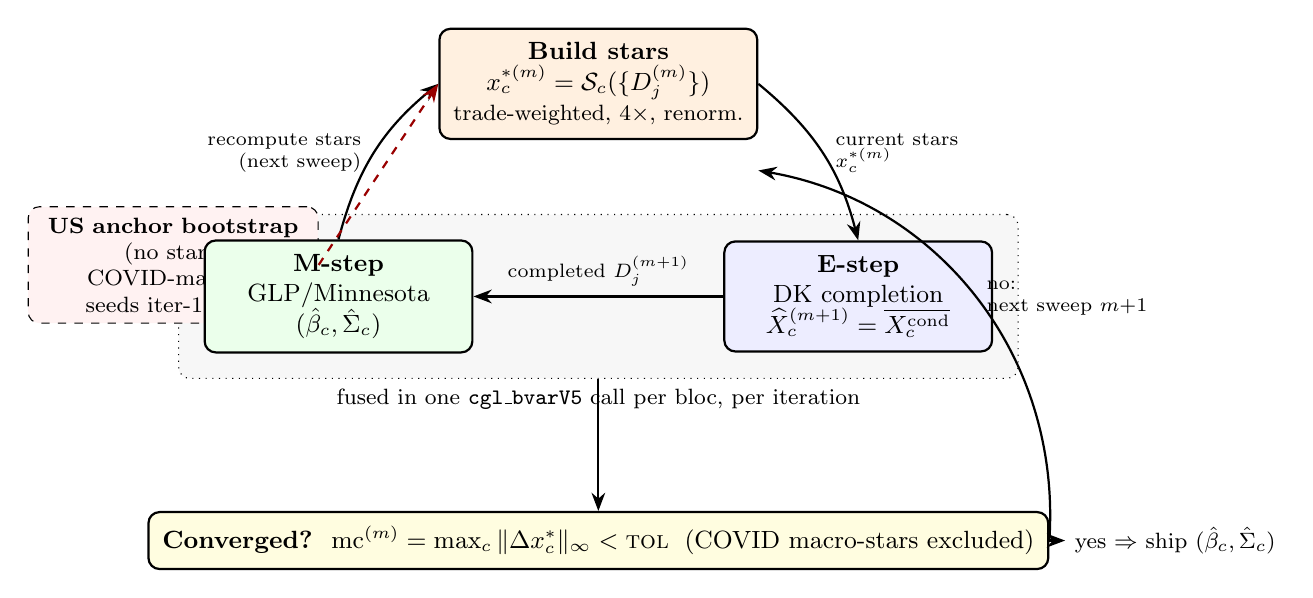
\begin{tikzpicture}[
  >=Stealth,
  font=\small,
  embox/.style={draw, rounded corners, thick, align=center, inner sep=5pt,
               minimum width=34mm, minimum height=13mm},
  estep/.style={embox, fill=blue!7},
  mstep/.style={embox, fill=green!8},
  starbox/.style={embox, fill=orange!12, minimum width=40mm},
  seed/.style={draw, dashed, rounded corners, align=center, inner sep=4pt,
               fill=red!5, font=\footnotesize, text width=34mm},
  flow/.style={->, thick},
]
  % seed
  \node[seed] (seed) at (-5.4,0)
    {\textbf{US anchor bootstrap}\\(no stars, COVID-masked)\\ seeds iter-1 stars};

  % star build
  \node[starbox] (stars) at (0,2.3)
    {\textbf{Build stars}\\$x^{*(m)}_c=\mathcal{S}_c(\{D^{(m)}_j\})$\\
     \footnotesize trade-weighted, $4\times$, renorm.};

  % E-step
  \node[estep] (E) at (3.3,-0.4)
    {\textbf{E-step}\\DK completion\\$\widehat X^{(m+1)}_c=\overline{X^{\text{cond}}_c}$};

  % M-step
  \node[mstep] (M) at (-3.3,-0.4)
    {\textbf{M-step}\\GLP/Minnesota\\$(\hat\beta_c,\hat\Sigma_c)$};

  % fused box around E and M
  \begin{scope}[on background layer]
    \node[draw, dotted, rounded corners, fit=(E)(M), inner sep=9pt,
          fill=black!3, label={[font=\footnotesize]below:%
          {fused in one \texttt{cgl\_bvarV5} call per bloc, per iteration}}] (fuse) {};
  \end{scope}

  % cyclic flow:  stars -> E -> (completed panels) -> M & stars rebuild
  \draw[flow] (stars.east) to[bend left=18]
     node[right, font=\scriptsize, align=left, xshift=1pt]
       {current stars\\ $x^{*(m)}_c$} (E.north);
  \draw[flow] (E.west) --
     node[above, font=\scriptsize] {completed $D^{(m+1)}_j$} (M.east);
  \draw[flow] (M.north) to[bend left=18]
     node[left, font=\scriptsize, align=right, xshift=-1pt]
       {recompute stars\\(next sweep)} (stars.west);
  \draw[flow, red!60!black, dashed] (seed.east) -- (stars.west);

  % convergence test
  \node[draw, rounded corners, thick, fill=yellow!12, inner sep=5pt,
        align=center] (conv) at (0,-3.5)
    {\textbf{Converged?}\;
     $\mathrm{mc}^{(m)}=\max_c\|\Delta x^{*}_c\|_{\infty}<\textsc{tol}$
     \;(COVID macro-stars excluded)};
  \draw[flow] (fuse.south) -- (conv.north);
  \draw[flow] (conv.east) to[bend right=42]
     node[right, font=\scriptsize, align=left] {no:\\ next sweep $m{+}1$} (stars.east |- 0,1.2);
  \node[right=2mm of conv, font=\footnotesize] (out)
    {yes $\Rightarrow$ ship $(\hat\beta_c,\hat\Sigma_c)$};
  \draw[flow] (conv.east) -- (out.west);
\end{tikzpicture}
\caption{The estimation-time EM fixed-point loop over the completed star
variables. A one-shot US anchor bootstrap (red, dashed) seeds the first
iteration's stars. Each iteration then (i) builds every receiver's
trade-weighted stars from the frozen start-of-iteration completed partner panels,
(ii) runs the \emph{fused} E-step (Durbin--Koopman posterior-mean completion of
the bloc's missing cells, \texttt{mean(Xcond,3)}) and M-step (GLP/Minnesota
Bayesian re-estimation) inside one \texttt{cgl\_bvarV5} call per bloc, and (iii)
recomputes the stars from the refreshed completions for the next Jacobi sweep.
The loop stops when the sup-norm change in the estimation stars falls below
$\textsc{tol}=0.03$ (with the COVID-imputed macro-star cells excluded as
Monte-Carlo noise), capped at $\textsc{maxit}=12$. This is distinct from the
solve-time deviation fixed point $x=Mx+d$ (Fig.~\ref{fig:coupling}), which runs
online with these coefficients frozen.}
\label{fig:gvar-em}
\end{figure}

Algorithm~\ref{alg:gvar-em} states the loop
(\texttt{pipeline/export\_bvar\_gvar24\_loop.m}; the credit-validation driver
\texttt{credit\_validate\_loop.m} carries an identical loop).

\begin{algorithm}[!ht]
\caption{EM fixed-point estimation of the coupled GVAR (completion of the star
variables; \texttt{export\_bvar\_gvar24\_loop.m}).}
\label{alg:gvar-em}
\algIn{per-bloc observed domestic panels with \texttt{NaN} holes (ragged edges,
COVID macro mask, short credit series); trade weights $W$; eligibility rules
(rate-less, hyperinflation, China nominal-GDP deflation);
\texttt{US\_ENDOGENOUS} flag; $\textsc{maxit}=12$; $\textsc{tol}=0.03$.}
\algOut{per-bloc posterior-mean models $\{(\hat\beta_c,\hat\Sigma_c)\}$ and
coefficient draws; converged completed stars $\{x^{*}_c\}$; iteration count.}
\begin{algsteps}
\item \algComment{US anchor bootstrap (once).} Complete the US domestic panel with \emph{no} stars (COVID macro cells \texttt{NaN}'d), $\widehat X_{\text{US}}\!=\!\overline{X^{\text{cond}}_{\text{US}}}$; set $D^{(0)}_{\text{US}}\!=\!\texttt{panelfrom}(\widehat X_{\text{US}})$. \algKw{if} \texttt{US\_ENDOGENOUS} then US joins the swept set; \algKw{else} $\text{rowB}\!=\!\text{blocs}(2{:}\text{end})$ (US frozen).
\item \algKw{for} $m=1$ \algKw{to} $\textsc{maxit}$:
\item \algInd \algComment{Jacobi sweep: stars built from the FROZEN $\{D^{(m-1)}_j\}$.}
\item \algInd \algKw{parfor} each swept bloc $c$:
\item \algIndd $x^{*}_c \gets \mathcal{S}_c(\{D^{(m-1)}_j\})$ \algComment{\texttt{buildstars}: trade-weighted, $4\times$ macro / level fin, per-quarter renorm, lead-\texttt{NaN} back-fill.}
\item \algIndd $X_c \gets [\,D^{\text{obs}}_c \mid x^{*}_c\,]$; apply COVID macro mask (domestic macro cols $+$ \texttt{ROWDEM},\texttt{ROWINF}; \texttt{ROWFIN} observed).
\item \algIndd $X^{\text{cond}}_c,\{\beta^{(g)}_c,\Sigma^{(g)}_c\} \gets \texttt{cgl\_bvarV5}(X_c,\dots)$ \algComment{E$+$M fused: DK completion $\,+\,$ GLP/MH draws.}
\item \algIndd $\widehat X_c \gets \overline{X^{\text{cond}}_c}=\texttt{mean(Xcond,3)}$;\quad $D^{(m)}_c \gets \texttt{panelfrom}(\widehat X_c)$;\quad store $(\hat\beta_c,\hat\Sigma_c)$ and draws.
\item \algInd \algComment{after the parfor:} commit $\{D^{(m)}_c\}$ so the next sweep's \texttt{buildstars} sees them.
\item \algInd \algComment{Convergence.} $\mathrm{mc} \gets \max_c \|x^{*(m)}_c - x^{*(m-1)}_c\|_{\infty}$ with COVID macro-star cells \texttt{NaN}'d.
\item \algInd \algKw{if} $m>1$ \algKw{and} $\mathrm{mc}<\textsc{tol}$: \algKw{break} (\textsc{converged}).
\item \algKw{return} $\{(\hat\beta_c,\hat\Sigma_c)\}$, draws, $\{x^{*}_c\}$, $m$.
\end{algsteps}
\end{algorithm}

\paragraph{Contrast with classical fixed-weight OLS GVAR.} The textbook GVAR of
\citet{PesaranSchuermannWeiner2004} and \citet{DeesDiMauroPesaranSmith2007}
(surveyed by \citealp{ChudikPesaran2016}) differs from this estimator on every
axis, and the differences are exactly the contribution.
\begin{enumerate}[label=(\arabic*)]
  \item \textbf{Iteration vs.\ single pass.} Classical GVAR builds each foreign
    star $x^{*}_{it}=\sum_j w_{ij}x_{jt}$ \emph{once} from observed partner data,
    treats it as weakly exogenous, and estimates each country VARX$^{*}$ in a
    single OLS (or reduced-rank ML) pass---no re-aggregation, no feedback into the
    stars. Here the stars are recomputed from model-completed panels every sweep
    and iterated to the fixed point~\eqref{eq:em:outer}.
  \item \textbf{Missing-data completion vs.\ truncation.} Classical GVAR requires
    a \emph{balanced} panel: ragged edges are dropped and the sample is truncated
    to the common span, with no imputation. Here the panel is unbalanced by
    design, and the Durbin--Koopman simulation smoother imputes the missing cells
    (ragged starts/ends, COVID macro mask, short credit) conditional on the
    observed cells---and crucially the imputed posterior means \emph{flow into the
    stars}, which is precisely what makes the iteration necessary.
  \item \textbf{Per-quarter renormalized weights.} Trade weights are fixed (IMF
    IMTS, 2021--2023), as in classical GVAR, \emph{but} they are renormalized per
    quarter and per component over the partners actually present and eligible,
    with hyperinflation and rate-less exclusions and China's nominal-GDP
    deflation---an unbalanced-panel device absent from the fixed-weight formula.
  \item \textbf{Bayesian posterior vs.\ OLS point estimates.} Each bloc is a
    hierarchical GLP/Minnesota BVAR with Metropolis-sampled hyperparameters,
    yielding a posterior (draws $\to$ predictive bands) and a per-variable
    random-walk-vs-white-noise prior choice, not OLS point estimates on a single
    balanced sample.
  \item \textbf{Jointly solved linkages.} The GVAR linkages and the estimation are
    solved \emph{jointly} here---the stars are a fixed point of the completion
    loop---whereas classical GVAR fixes the stars pre-estimation and stacks the
    country models into a single global linear system only afterwards.
\end{enumerate}
In one line: the novelty is a \emph{Durbin--Koopman data-augmentation completion
of unbalanced, COVID-masked partner panels, feeding a per-quarter-renormalized
trade-weighted star aggregation, inside a Bayesian per-bloc re-estimation,
iterated to a star fixed point}---so the cross-country linkages are an estimated
object rather than a fixed pre-estimation input. The frozen posterior means it
produces are what the solve-time coupling of
Section~\ref{sec:gvar:fixedpoint} then propagates.

\subsection{Coupling at solve time, not estimation}\label{sec:gvar:fixedpoint}

\begin{figure}[!ht]
  \centering
  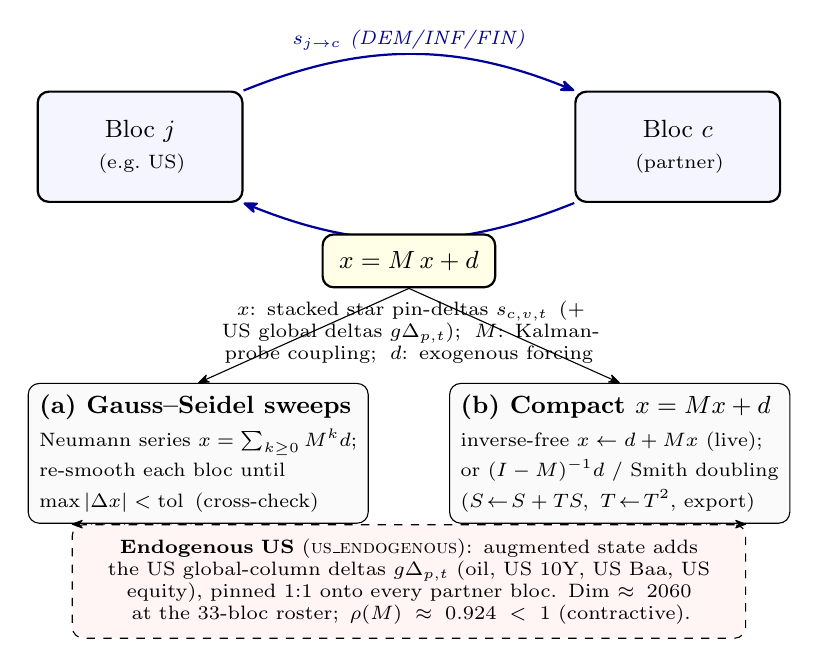
\begin{tikzpicture}[
    >={Stealth[round]},
    font=\small,
    bloc/.style={draw, rounded corners, minimum width=26mm, minimum height=14mm,
                 align=center, thick, fill=blue!4},
    route/.style={draw, rounded corners, minimum width=42mm, align=left,
                  inner sep=4pt, fill=black!2},
    star/.style={font=\scriptsize\itshape, fill=white, inner sep=1pt},
  ]
    % --- two coupled blocs (the cycle) ---
    \node[bloc] (j) {Bloc $j$\\\scriptsize\,(e.g.\ US)};
    \node[bloc, right=42mm of j] (c) {Bloc $c$\\\scriptsize\,(partner)};

    % star-pin feedback cycle j <-> c
    \draw[->, thick, blue!60!black] (j.north east) to[bend left=22]
      node[star, above] {$s_{j\to c}$ (DEM/INF/FIN)} (c.north west);
    \draw[->, thick, blue!60!black] (c.south west) to[bend left=22]
      node[star, below] {$s_{c\to j}$} (j.south east);

    % --- fixed-point equation ---
    \coordinate (jc) at ($(j)!0.5!(c)$);
    \node[below=11mm of jc, draw, rounded corners, thick,
          fill=yellow!10, inner sep=6pt] (eq)
      {$\displaystyle x = M\,x + d$};
    \node[below=1pt of eq, font=\scriptsize, align=center, text width=58mm]
      {$x$: stacked star pin-deltas $s_{c,v,t}$ \,(+ US global deltas $g\Delta_{p,t}$);
       \;$M$: Kalman-probe coupling; \;$d$: exogenous forcing};

    % --- two solution routes ---
    \node[route, below left=12mm and -6mm of eq] (gs)
      {\textbf{(a) Gauss--Seidel sweeps}\\[1pt]
       \scriptsize Neumann series $x=\sum_{k\ge0}M^{k}d$;\\
       \scriptsize re-smooth each bloc until\\
       \scriptsize $\max|\Delta x|<\text{tol}$\, (cross-check)};
    \node[route, below right=12mm and -6mm of eq] (dir)
      {\textbf{(b) Compact $x = M x + d$}\\[1pt]
       \scriptsize inverse-free $x\leftarrow d+Mx$ (live);\\
       \scriptsize or $(I-M)^{-1}d$ / Smith doubling\\
       \scriptsize ($S\!\leftarrow\!S+TS,\ T\!\leftarrow\!T^{2}$, export)};
    \draw[->] (eq.south) -- (gs.north);
    \draw[->] (eq.south) -- (dir.north);

    % --- endogenous-US annotation ---
    \coordinate (gsdir) at ($(gs)!0.5!(dir)$);
    \node[draw, dashed, rounded corners, below=9mm of gsdir,
          fill=red!4, inner sep=5pt, align=center, text width=82mm, font=\scriptsize] (us)
      {\textbf{Endogenous US} (\textsc{us\_endogenous}): augmented state adds the US
       global-column deltas $g\Delta_{p,t}$ (oil, US 10Y, US Baa, US equity),
       pinned $1{:}1$ onto every partner bloc.
       Dim $\approx 2060$ at the $33$-bloc roster; \,$\rho(M)\approx 0.924<1$ (contractive).};
    \draw[->, dotted] (gs.south) -- (us.north west);
    \draw[->, dotted] (dir.south) -- (us.north east);
  \end{tikzpicture}
  \caption{Solve-time cross-country coupling as the affine fixed point
    $x = M\,x + d$. Two coupled blocs exchange trade-weighted star pin-deltas
    (DEM/INF/FIN), forming the feedback cycle; the deviation state $x$ stacks
    these pins (plus the US global-column deltas under an endogenous US). The
    fixed point admits two equivalent solutions---(a) Gauss--Seidel/Neumann
    sweeps through the Durbin--Koopman smoother, used as the cross-check, and (b)
    the compact $M$-state recursion, solved inverse-free by the Neumann
    fixed-point $x\leftarrow d+Mx$ on the production path (the explicit
    $(I-M)^{-1}d$ / Smith doubling are reserved for the small frozen-anchor case
    and the export-time precompute, since the in-browser $O(\dim^{3})$ inverse is
    prohibitive at $\dim\approx 2060$). With the US endogenous the augmented
    state has dimension $\approx 2060$ and spectral radius
    $\rho(M)\approx 0.924<1$, so the iteration contracts and the two routes agree
    to $\sim 10^{-9}$.}
  \label{fig:coupling}
\end{figure}

Because each bloc is estimated independently, there is no joint, block-exogenous
GVAR system; the cross-country linkage is imposed when the scenario is solved.
The key observation is that, with coefficients fixed at their posterior mean
$(\hat\beta, \hat\Sigma)$, the conditional-forecast operator of
Section~\ref{sec:kalman} is \emph{affine} in the conditioning values (the
Kalman filter and Durbin--Koopman smoother are linear in the pinned data). The
\emph{baseline} forecast of each bloc is therefore data-driven and computed
exactly once, via an all-\texttt{NaN} (unconditional) smoother pass; only the
scenario \emph{deviation} couples across blocs.

Because the US is now endogenous it is no longer held outside the fixed point,
and the compact deviation state is correspondingly \emph{augmented}. It collects
(i) the star pin-deltas $s_{c,v,t}$ of \emph{every} coupled bloc $c$---the US
included---for star variable $v\in\{\text{DEM},\text{INF},\text{FIN}\}$ at
horizon $t$, and (ii) the per-period \emph{deviation of each US global column}
$g\Delta_{p,t}$, which under the frozen-anchor design was a constant and is now
itself part of the unknown. Stacking these into a vector $x$, the deviation
system is the linear fixed point
\begin{equation}\label{eq:gvar:fp}
  x = M\,x + d,
\end{equation}
where $d$ is the exogenous forcing (each bloc's own scenario pins moving its
linked series at zero partner and global delta) and $M$ now carries three
coupling families: star~$\leftarrow$~star (receiver $c$'s star responds to a
partner $j$'s free-variable path---with the US participating both as partner and
as receiver), the US-global definition rows (a global column's deviation as the
US's own response to its star pins), and star~$\leftarrow$~global (a partner's
star responds to its own global pin). The US-determined globals therefore live
\emph{inside} $M$ rather than in $d$, which is precisely the new RoW$\to$US
feedback loop. The augmented state has dimension $\approx 2060$ at the full
$33$-bloc roster.

The fixed point~\eqref{eq:gvar:fp} is solved two equivalent ways:
\begin{enumerate}[label=(\alph*)]
  \item \textbf{Gauss--Seidel / Neumann sweeps} (the cross-check) sum the
    Neumann series $x = \sum_{k\ge 0} M^k d$ by re-conditioning each bloc in turn
    through the Durbin--Koopman smoother \citep{DurbinKoopman2002,
    DurbinKoopman2012} until the maximum level change falls below tolerance.
  \item \textbf{Direct closed form}
    \begin{equation}\label{eq:gvar:closed}
      x = (I - M)^{-1} d,
    \end{equation}
    after which one final conditional-forecast pass per bloc reconstructs the
    full set of free variables consistent with the converged pin-deltas.
\end{enumerate}
At the full $33$-bloc endogenous-US configuration the spectral radius is
$\rho(M)\approx 0.924 < 1$, so the Neumann series converges and $(I-M)$ is
nonsingular; the two solvers agree to $\sim 10^{-9}$. (The legacy frozen-anchor
RoW-only operator had a smaller radius, $\rho(M)\approx 0.726$; closing the
RoW$\to$US loop raises the coupling but leaves the system comfortably
contractive.)

Algorithm~\ref{alg:coupling} states both solve paths
(\texttt{app/src/lib/compute/gvarSolve.ts}). The coupling operator $M$
is never formed by writing down a joint VAR; each of its columns is
\emph{probed} by perturbing one pinned cell and reading the affine
conditional-forecast response of every linked bloc through the
Durbin--Koopman smoother---so $M$ encodes the same per-bloc Kalman
operator that produces the baseline, restricted to the deviation.

\begin{algorithm}[!ht]
\caption{Solve-time coupling fixed point $x=Mx+d$ (Gauss--Seidel/Neumann
and direct $(I-M)^{-1}$; \texttt{gvarSolve.ts}).}
\label{alg:coupling}
\algIn{per-bloc posterior-mean models $\{(\hat\beta_c,\hat\Sigma_c)\}$;
scenario pins; trade weights $W$; \texttt{US\_ENDOGENOUS} flag; tolerance
$\textsc{tol}$.}
\algOut{converged deviation state $x$ and per-bloc scenario deltas $\texttt{delta}[c]$; sweep count; $\rho(M)$.}
\begin{algsteps}
\item \algComment{Forcing.} Build $d$: each bloc's own scenario pins, evaluated at \emph{zero} partner-star and global deltas (one DK conditional-forecast pass per pinned bloc).
\item \algComment{Coupling families in $M$ (endogenous-US augmented state).} star$\leftarrow$star (a receiver's star responds to a partner's free path; the US is both partner and receiver); US-global rows ($g\Delta$ as the US's own response to its star pins); star$\leftarrow$global (a partner star responds to its own global pin).
\item \algKw{Path A --- Gauss--Seidel / Neumann sweeps (inverse-free).}
\item \algInd $x\gets d$
\item \algInd \algKw{repeat} (sweep): \algKw{for each} coupled bloc $c$ (US included \algKw{if} \texttt{US\_ENDOGENOUS}): re-condition $c$ through the DK smoother on the current partner-star and global deltas $\Rightarrow$ update $x$'s block for $c$.
\item \algIndd \algComment{this sums the Neumann series $x=\sum_{k\ge0}M^k d$ term by term.}
\item \algInd \algKw{until} $\max|\Delta x| < \textsc{tol}$; record $\rho_{\text{emp}}$ from the geometric residual decay.
\item \algKw{Path B --- direct closed form (cached).}
\item \algInd assemble $M$ by probing columns; \algKw{if} a precomputed $(I-M)^{-1}$ matches the model signature \& pin structure, hydrate it; \algKw{else} fall back to Path A (the dense in-browser inverse is never built live).
\item \algInd $x \gets (I-M)^{-1} d$; one final per-bloc DK pass reconstructs all free variables consistent with the converged pin-deltas.
\item \algComment{Cross-check.} The two paths agree to the verified tolerance ($\max|\Delta|<10^{-4}$ across all blocs in the closed-form vs.\ iterative regression tests, with the iterative reference itself converged to $10^{-7}$), confirming $\rho(M)<1$; report $\rho(M)$ via power iteration on $M$ (in practice on $M^2$, see Sec.~\ref{sec:gvar:solvemode}).
\item \algKw{return} $x$, $\texttt{delta}[c]$, sweep count, $\rho(M)$.
\end{algsteps}
\end{algorithm}

A practical consequence drives the deployment. The operator $M$ depends on the
estimated models and on the conditioning \emph{structure} (which cells are
pinned) but \emph{not} on the pinned \emph{values}, so it can be assembled once
and reused for every value change during interactive dragging. Its dense inverse
is, however, expensive: at the augmented endogenous dimension ($\approx 2060$)
the naive in-browser inversion would take tens of minutes (the cubic inverse is
of order three-quarters of an hour), making a cold build infeasible even in a
Web Worker. The tool therefore \textbf{ships a precomputed coupling artifact}
(\texttt{coupling\_default.json.gz}) containing $M$, $(I-M)^{-1}$, and $\rho(M)$
for the default (empty) pin structure, with the inverse computed offline by a
high-performance \textsc{blas} routine. The artifact is large (the dense
$2060\times2060$ inverse), so it is shipped \emph{gzipped} (about $30$\,MB
compressed) and decompressed in the browser via the native
\texttt{DecompressionStream} API at load. This artifact is mandatory, not an
optimization: hydrating it reduces the first complete solve from the
tens-of-minutes cold build to a few seconds. A model-signature gate guards
against using a stale inverse after any re-estimation; a genuinely novel pin
structure misses the cache and falls back to an inverse-free Neumann solve
(the in-browser cubic inverse is never built live).

\subsection{Two-tier solve: live preview vs.\ the full fixed point}\label{sec:gvar:solvemode}

The endogenous US makes the \emph{complete} cross-country solve materially more
expensive than the legacy frozen-anchor solve, because placing or moving a US
pin re-probes the (large) US bloc, the heavy step. To keep the interface
reactive the tool exposes \textbf{two solve tiers}:
\begin{itemize}
  \item \textbf{Direct preview} (the default while dragging). A fast,
    first-order approximation that propagates the scenario through the
    pre-warmed local per-bloc elasticities---one cross-country hop, without the
    full multiplier feedback---so the propagated paths update live as the user
    drags a pin. The per-bloc response kernels are cached by model signature and
    own-pin structure, so a value-only re-drag (same pinned cells) reuses them
    and re-solves cheaply; a \emph{structure} change (pinning a new cell) re-probes
    the US bloc and is the slower direct step (a few seconds), during which a
    small ``computing\ldots'' pill is shown so the wait does not look like a
    freeze.
  \item \textbf{Full GVAR} (on demand). The complete fixed point of
    \eqref{eq:gvar:fp}---all feedback loops, including RoW$\to$US---computed when
    the user clicks the \textbf{Solve full GVAR} button. This consumes the
    hydrated $(I-M)^{-1}$ artifact and takes a few seconds.
\end{itemize}
A badge above the charts reports which tier produced the current result---an
amber ``GVAR DIRECT preview'' versus a blue ``GVAR full solve''---together with
the sweep count, the spectral radius $\rho$, and the solve time. When a DIRECT
preview is on screen, the \textbf{Solve full GVAR} button is offered to upgrade
it to the complete fixed point. Drag-release dispatch and debouncing keep the
preview channel from firing mid-drag, and the heavy coupling artifact is stripped
from the worker messages on the direct path (it is only needed for the full
solve). For the legacy frozen-anchor topology---or any deployment where the US is
not endogenous---both tiers resolve to the same already-fast cached closed form,
so the two-tier distinction is invisible there.

\subsection{Global commons: US-determined common shocks}\label{sec:gvar:commons}

The headline addition of version~2.0 is a set of four \emph{global common}
variables that are determined by the United States but carried by \emph{every}
bloc:
\begin{itemize}
  \item \texttt{GLB\_OIL} --- the spot oil price (WTI);
  \item \texttt{GLB\_USLR} --- the US 10-year Treasury yield;
  \item \texttt{GLB\_USBAA} --- the US Baa corporate-bond yield (a credit-spread
    proxy);
  \item \texttt{GLB\_USEQ} --- US equity prices.
\end{itemize}
In the US bloc these enter as ordinary \emph{endogenous} variables; in each
partner bloc the same four identifiers (matched one-to-one by \emph{name}, never
by position) are carried as weakly-exogenous commons that the solver \emph{pins}.

The pinning is by \emph{deviation}, not by level. Each partner bloc $c$ sets each
global column to its own baseline plus the US deviation of the matching global,
\begin{equation}\label{eq:gvar:globalpin}
  \widehat{\text{GLB}}_{c,t}
  = \bar{\text{GLB}}_{c,t}
    + \bigl(\text{GLB}^{\text{scen}}_{\text{US},t}
      - \bar{\text{GLB}}_{\text{US},t}\bigr),
\end{equation}
where $\bar{(\cdot)}$ denotes the bloc's own unconditional baseline. This is a
load-bearing design choice. Each RoW bloc estimated its \emph{own} baseline path
for the globals as weakly-exogenous regressors, and those baseline levels differ
from the US's by tens of $100\ln$ units (for example, of order $+17$, $+70$, and
$+28$ for the euro area, Japan, and China on oil). Pinning the US \emph{level}
would inject that entire baseline gap as a spurious deviation the instant a bloc
is selected, even under a zero scenario. Pinning the US \emph{deviation} on top
of each bloc's own baseline instead yields exactly zero spillover at a zero
scenario and an \emph{identical} common shock under conditioning---precisely
mirroring the star convention $\bar{\text{RoW}} + \text{partner-delta}$
of~\eqref{eq:gvar:star_growth}--\eqref{eq:gvar:star_fin}. A US oil pin therefore
propagates the same oil deviation to all $32$ partner blocs (verified to within
$10^{-9}$), while each bloc's domestic variables respond through its \emph{own}
estimated coefficients.

Mechanically, with the US now endogenous the US global \emph{deviation} is itself
an unknown of the fixed point rather than a frozen constant. The global columns
therefore enter the \emph{augmented} coupling operator $M$ of
Section~\ref{sec:gvar:fixedpoint}: a US-global definition row writes each
global's deviation as the US's own response to its star pins, and a
star~$\leftarrow$~global block routes each partner's global pin back into its
stars. This is exactly the channel by which a partner shock now feeds back to the
US. Indirect effects---a common shock moving a bloc's macroeconomy, which moves
its stars, which spill to other blocs---flow through the same operator and are
not double-counted. A bloc that carries no globals reduces the pin to a no-op,
leaving the legacy globals-free solve byte-identical.

On the user interface the globals are \emph{conditionable} on the US screen
(where they are endogenous) and \emph{read-only}, carried over from the US path,
on every other bloc.

\subsection{Relation to the fiscal and counterfactual layers}\label{sec:gvar:layers}

The GVAR layer composes with the single-country machinery rather than replacing
it. The displayed scenario line for an active GVAR bloc is the cross-country
propagated path of this section; for a standalone (non-GVAR) economy it is the
single-country conditional forecast of Section~\ref{sec:kalman}. The US derived
fiscal block (the debt-to-GDP accounting identity, whose empirical motivation is
the fiscal reaction function of \citealp{Bohn1998}) and the DSGE policy
counterfactual---including the \citet{BarnichonMesters2023} optimal-policy
problem---continue to operate on the US bloc's propagated path. Conditional
forecasts throughout use the large-cross-section state-space method of
\citet{BanburaGiannoneLenza2015} with the hierarchical prior of
\citet{Giannone2015}, applied independently to each bloc and stitched together
only through the linear deviation system~\eqref{eq:gvar:fp}.

\section{Fiscal Blocks: Estimated Drivers and Debt Accounting}\label{sec:fiscal}

Six of the economies in the tool---the United States, the Euro Area,
Japan, the United Kingdom, Canada, and China---carry a dedicated
\emph{fiscal block}.  The block follows the stock-flow-consistent
division of labour shared by the U.S.\ Congressional Budget Office's
conditional-BVAR budget mechanics and the IMF Financial Programming
(FPP) / debt-sustainability frameworks: the BVAR is used as a
\emph{macro-fiscal scenario generator} that jointly forecasts the
macroeconomy together with a small number of fiscal \emph{flow drivers},
while the public-debt stock and the headline reporting variables
(primary and overall balance, interest, debt-to-GDP, gross financing
needs) are \emph{derived outside the VAR} by the government
budget-constraint identity.  No reduced-form equation is ever allowed to
forecast the debt stock freely, because an unconstrained debt VAR is
explosive: the debt-dynamics identity has a near-unit autoregressive
root $(1+i)/(1+g^{n})$, and small parameter errors compound into
divergent debt paths.  Imposing the identity by construction is exactly
the discipline that the CBO and FPP/DSA frameworks demand, and it is the
structure implemented in
\texttt{app/src/lib/compute/fiscalAccounting.ts}.

\subsection{Estimated Fiscal Drivers}\label{sec:fiscal_drivers}

The BVAR jointly estimates the macro block of
Section~\ref{sec:variables} together with \emph{four} fiscal flow drivers,
all entering as linear (\texttt{lin}) variables:
\begin{itemize}
  \item \textbf{Revenue} (\texttt{FREV\_GDP}): general-government
    receipts as a percentage of GDP, an annual ratio.
  \item \textbf{Primary expenditure} (\texttt{FPEXP\_GDP}):
    non-interest outlays as a percentage of GDP, an annual ratio.
  \item \textbf{Effective interest rate} (\texttt{EFFI}, \% p.a.): the
    average rate the government actually pays on its outstanding stock,
    constructed as net interest divided by the lagged gross debt and
    annualized. Because the stock turns over only as maturing securities are
    refinanced, this effective rate lags market yields and is therefore
    distinct from---and estimated separately from---the policy rate and the
    market yields already in the macro block.
  \item \textbf{Stock-flow adjustment} (\texttt{SFA}, \% of GDP): the
    deficit--debt discrepancy described below.
\end{itemize}
The effective rate \texttt{EFFI} is the estimated interest driver of the
deployed block. (The parametrisation has changed over time: an early version
carried $\Delta(\text{debt}/\text{GDP})$ directly, and a later one carried debt
service to GDP \texttt{DSVC}; the current block reverts to the effective rate.)
The interest bill is then formed inside the accounting recursion as
$\mathit{int}_t = i^{\text{eff}}_t\, d_{t-1}/100$.

\paragraph{The stock-flow adjustment as an estimated variable.}
The novelty of the current block is that the stock-flow adjustment
(\texttt{SFA}) is now an \emph{estimated} BVAR variable rather than a constant
plug. It is the exact residual of the tool's own debt recursion---the part of
the observed change in gross debt that the flow side (deficit plus the
interest--growth ``snowball'') does \emph{not} explain. Economically this seam
arises because the headline deficit is measured on a federal-flows perimeter
while the debt stock is gross debt (so intragovernmental holdings, valuation
effects, and other below-the-line ``other means of financing'' operations move
the two apart). It is constructed so that it closes the recursion to machine
precision on history, and the pandemic quarters are set to missing
(\texttt{NaN}) so the COVID-as-missing Gibbs sampler imputes them
(Section~\ref{sec:covid}) rather than letting the 2020 swing contaminate the
estimate. Carrying \texttt{SFA} as a forecast variable means the
debt-to-GDP \emph{projection} now propagates its own \texttt{SFA} path forward
(with dynamics and uncertainty bands) instead of defaulting the discrepancy to
zero, which materially affects the high-debt blocs whose historical SFA is large
and persistent. The historical SFA means (in \% of GDP), which each bloc also
ships as its \texttt{sfaDefault} fallback, are: US $1.75$, EA $0.33$, JP $2.23$,
UK $3.15$, CA $3.19$, CN $4.02$.

Because all four drivers are ordinary BVAR variables, they inherit the full
estimation machinery of Sections~\ref{sec:bvar}--\ref{sec:kalman}: the
hierarchical Minnesota prior \citep{Giannone2015}, the COVID-as-missing
data-augmentation Gibbs treatment, the companion-form Durbin--Koopman
conditional smoother \citep{DurbinKoopman2002, DurbinKoopman2012}, and the
\citet{BanburaGiannoneLenza2015} conditioning-via-partial-observations
construction.  In the five Global-VAR fiscal blocs (EA, JP, UK, CA, CN)---and
now in the endogenous US bloc itself---the fiscal drivers are part of the
domestic block and propagate to the other economies through the shared
Rest-of-World stars, exactly as the macro variables do
\citep{PesaranSchuermannWeiner2004, DeesDiMauroPesaranSmith2007}.

\paragraph{A stationary prior for the fiscal ratios.} The three
GDP-ratio drivers---revenue \texttt{FREV\_GDP}, primary expenditure
\texttt{FPEXP\_GDP}, and the stock-flow adjustment \texttt{SFA}---are
mean-reverting shares that fluctuate around a roughly constant
in-sample level; they are \emph{not} integrated. Carrying them under the
default random-walk own-lag prior ($\delta=1$) is therefore the wrong
null: it injects a built-in drift that lets the projected ratio wander
away from its historical level at the long end of the horizon. These
three drivers are accordingly tagged \texttt{prior:"WN"} in every fiscal
bloc's specification and estimated with the \emph{stationary}
white-noise own-lag prior ($\delta=0$) of Section~\ref{sec:ownlag}: the
estimator collects them via \(\texttt{pos}=\texttt{find}(\texttt{prior}==
\text{`}\texttt{WN}\text{'})\) and passes the set as the
\texttt{stationary} argument of \texttt{cgl\_bvarV5}, so
\(\texttt{diagb}(\texttt{pos})=0\) centers their own-lag dynamics on
mean reversion to the equation constant. The effective interest rate
\texttt{EFFI}, by contrast, \emph{retains} the random-walk prior: it is a
slow-moving stock-average rate (net interest over lagged debt) whose
level is genuinely persistent---it turns over only as maturing securities
refinance---so a near-unit own-lag is the right prior null for it.

The empirical effect is exactly the intended one. Under the random-walk
prior the U.S.\ revenue ratio was pinned near its end-of-sample value
($\sim 19\%$) and drifted from there; under the white-noise prior it now
\emph{reverts} to its $\sim 17.4\%$ in-sample mean over the projection,
and the expenditure ratio and \texttt{SFA} likewise return to their
historical means rather than carrying the last observation forward
indefinitely. We emphasise (per Section~\ref{sec:ownlag}) that this is a
shift of the prior \emph{center}, not a hard stationarity constraint: the
posterior own-lag coefficient is still the GLP prior--likelihood balance
at the estimated tightness $\lambda$, so a fiscal ratio whose data
genuinely trend will still be allowed to do so---the \texttt{WN} prior
only removes the mechanical drift that the random-walk center would
otherwise build in. Because \texttt{pos} is empty for the $44$ non-fiscal
blocs, this change is a no-op (byte-identical output) everywhere except
the six fiscal blocs.

Each fiscal bloc ships a \texttt{fiscal\_meta.json} file that pins the
column layout used by the accounting recursion.  It carries the integer
indices $\texttt{idx} = \{\texttt{gdp}, \texttt{deflator},
\texttt{revenue}, \texttt{primaryExp}, \texttt{effRate}, \texttt{sfa}\}$
into the level-space forecast matrix---the first two locate the real-GDP and
deflator log-levels that supply nominal growth, the next two locate the
revenue and primary-expenditure drivers, $\texttt{effRate}$ locates the
estimated effective-rate column, and $\texttt{sfa}$ locates the estimated
stock-flow-adjustment column---together with the seed debt ratio $d_0$ and a
fallback \texttt{sfaDefault} (e.g.\ the U.S.\ block has $d_0 = 122.57$,
$\texttt{idx.effRate} = 35$, $\texttt{idx.sfa} = 36$, and
$\texttt{sfaDefault} = 1.75$; the U.K.\ block has $d_0 = 96.24$,
$\texttt{idx.effRate} = 18$, $\texttt{idx.sfa} = 19$). The presence of
$\texttt{idx.sfa}$ is the switch that selects the per-quarter estimated SFA:
when it is set, \texttt{computeFiscalBlock} reads the forecast SFA off that
column so the debt projection carries the discrepancy forward with its own
dynamics and bands; when it is unset, the recursion falls back to the constant
\texttt{sfaDefault} (or zero). A legacy block that instead carried an
$\texttt{idx.debtService}$ column would read that column directly as the period
interest flow and back out the effective rate; the current effective-rate blocks
do not.

\subsection{The Budget-Identity Recursion}\label{sec:fiscal_identity}

\begin{figure}[!ht]
\centering
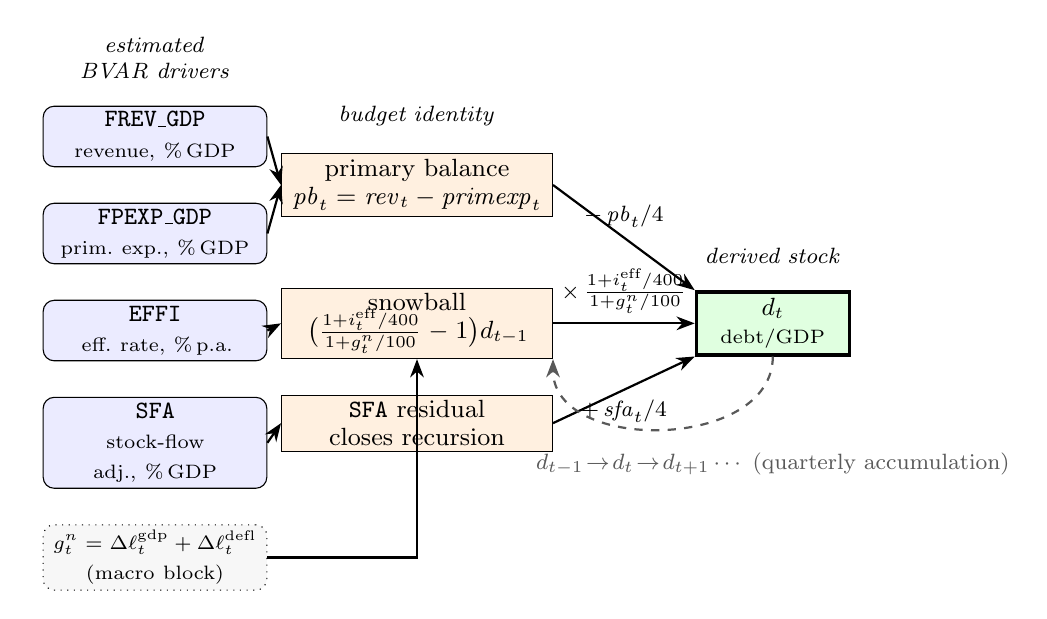
\begin{tikzpicture}[
    >=Stealth, node distance=4.5mm,
    font=\small,
    driver/.style={draw, rounded corners, fill=blue!8, minimum height=6.5mm,
                   text width=27mm, align=center, inner sep=2pt},
    iden/.style={draw, fill=orange!12, minimum height=6.5mm,
                 text width=33mm, align=center, inner sep=2pt},
    stock/.style={draw, very thick, fill=green!12, minimum height=8mm,
                  text width=18mm, align=center, inner sep=2pt},
    op/.style={font=\footnotesize},
    flow/.style={->, thick},
    lag/.style={->, dashed, thick, gray!70!black}
  ]

  % --- Estimated BVAR drivers (left column) ---
  \node[driver] (rev)  {\texttt{FREV\_GDP}\\\scriptsize revenue, \%\,GDP};
  \node[driver, below=of rev]  (exp) {\texttt{FPEXP\_GDP}\\\scriptsize prim.\ exp., \%\,GDP};
  \node[driver, below=of exp]  (eff) {\texttt{EFFI}\\\scriptsize eff.\ rate, \%\,p.a.};
  \node[driver, below=of eff]  (sfa) {\texttt{SFA}\\\scriptsize stock-flow adj., \%\,GDP};

  \node[above=2.2mm of rev, font=\footnotesize\itshape, text width=30mm, align=center]
       {estimated BVAR drivers};

  % --- Budget-identity terms (middle column) ---
  \coordinate (revexp) at ($(rev)!0.5!(exp)$);
  \node[iden, right=16mm of revexp] (pb)
       {primary balance\\[-1pt]$\mathit{pb}_t=\mathit{rev}_t-\mathit{primexp}_t$};
  \node[iden, below=9mm of pb] (snow)
       {snowball\\[-1pt]$\bigl(\tfrac{1+i^{\text{eff}}_t/400}{1+g^{n}_t/100}-1\bigr)d_{t-1}$};
  \node[iden, below=of snow] (res)
       {\texttt{SFA} residual\\[-1pt]closes recursion};

  \node[above=2.2mm of pb, font=\footnotesize\itshape, text width=34mm, align=center]
       {budget identity};

  % nominal growth feed (from macro block)
  \node[draw, dotted, rounded corners, fill=gray!6, text width=27mm, align=center,
        inner sep=2pt, below=of sfa]
       (gn) {\scriptsize $g^{n}_t=\Delta\ell^{\text{gdp}}_t+\Delta\ell^{\text{defl}}_t$\\(macro block)};

  % --- Debt stock recursion (right column) ---
  \node[stock, right=18mm of snow] (dt)
       {$d_t$\\[-1pt]\scriptsize debt/GDP};

  \node[above=2.2mm of dt, font=\footnotesize\itshape, text width=22mm, align=center]
       {derived stock};

  % driver -> identity flows
  \draw[flow] (rev.east) -- (pb.west);
  \draw[flow] (exp.east) -- (pb.west);
  \draw[flow] (eff.east) -- (snow.west);
  \draw[flow] (sfa.east) -- (res.west);
  \draw[flow] (gn.east) -| (snow.south);

  % identity -> stock recursion (terms of eq.~debt)
  \draw[flow] (pb.east)   -- node[op, above]{$-\,\mathit{pb}_t/4$} (dt.north west);
  \draw[flow] (snow.east) -- node[op, above]{$\times\,\tfrac{1+i^{\text{eff}}_t/400}{1+g^{n}_t/100}$} (dt.west);
  \draw[flow] (res.east)  -- node[op, below]{$+\,\mathit{sfa}_t/4$} (dt.south west);

  % --- accumulation across quarters: lagged debt feedback ---
  \draw[lag] (dt.south) .. controls +(0,-12mm) and +(0,-12mm) .. (snow.south east);
  \node[font=\footnotesize, gray!70!black, align=center, below=11mm of dt.south, anchor=north]
       {$d_{t-1}\!\rightarrow\! d_t\!\rightarrow\! d_{t+1}\cdots$ (quarterly accumulation)};

\end{tikzpicture}
\caption{Fiscal stock-flow schematic. The four estimated BVAR drivers
(\texttt{FREV\_GDP}, \texttt{FPEXP\_GDP}, \texttt{EFFI}, \texttt{SFA};
Section~\ref{sec:fiscal_drivers}) feed the budget identity: revenue and
primary expenditure form the primary balance $\mathit{pb}_t$
\eqref{eq:fiscal_pb}; the effective rate \texttt{EFFI} and nominal growth
$g^{n}_t$ \eqref{eq:fiscal_gn} form the interest--growth \emph{snowball}
\eqref{eq:fiscal_snowball}; and the estimated \texttt{SFA} enters as the
residual that closes the recursion. These flows accumulate into the derived
debt-to-GDP stock $d_t$ by the quarterized roll-forward
$d_t = d_{t-1}\,(1{+}i^{\text{eff}}_t/400)/(1{+}g^{n}_t/100)
- \mathit{pb}_t/4 + \mathit{sfa}_t/4$ \eqref{eq:fiscal_debt}, with the lagged
stock $d_{t-1}$ fed back each quarter (dashed). Debt is \emph{derived}, never
estimated (\texttt{computeFiscalBlock}, Section~\ref{sec:fiscal_identity}).}
\label{fig:fiscal}
\end{figure}

Let $d_t$ denote the debt-to-GDP ratio (in percent), $i^{\text{eff}}_t$
the effective rate (percent per annum), and $g^{n}_t$ nominal GDP growth
(percent per quarter).  All flows below are annual ratios in percent of
GDP.  Nominal growth is read directly off the level-space forecast as
the sum of the real-GDP and deflator log-differences, in the
$100\cdot\ln$ space of Section~\ref{sec:units}:
\begin{equation}\label{eq:fiscal_gn}
  g^{n}_t \;=\; \bigl(\ell^{\text{gdp}}_t - \ell^{\text{gdp}}_{t-1}\bigr)
            \;+\; \bigl(\ell^{\text{defl}}_t - \ell^{\text{defl}}_{t-1}\bigr),
\end{equation}
where $\ell$ is the stored $100\cdot\ln$ level and the right-hand side is
already in percent per quarter (it is not annualized by the factor of
four used for display in \eqref{eq:growth}).  The primary balance is the
revenue--expenditure gap (positive $=$ surplus),
\begin{equation}\label{eq:fiscal_pb}
  \mathit{pb}_t \;=\; \mathit{rev}_t \;-\; \mathit{primexp}_t,
\end{equation}
the interest bill (debt service) is the estimated effective rate applied to the
lagged debt stock,
\begin{equation}\label{eq:fiscal_int}
  \mathit{int}_t \;=\; i^{\text{eff}}_t\,\frac{d_{t-1}}{100},
\end{equation}
i.e.\ the BVAR forecast of the effective rate \texttt{EFFI} drives the interest
flow directly, with the lagged debt $d_{t-1}$ converting the rate into a
percent-of-GDP flow. (A legacy debt-service block would instead supply
$\mathit{int}_t$ as the estimated \texttt{DSVC} ratio and back out the effective
rate as $i^{\text{eff}}_t = 100\,\mathit{int}_t/d_{t-1}$.) The overall balance
and deficit follow as
\begin{equation}\label{eq:fiscal_bal}
  \mathit{ob}_t \;=\; \mathit{pb}_t - \mathit{int}_t,
  \qquad
  \mathit{def}_t \;=\; -\,\mathit{ob}_t \;=\; \mathit{int}_t - \mathit{pb}_t.
\end{equation}
The debt stock is then rolled forward one quarter by the
FPP/DSA debt-dynamics equation,
\begin{equation}\label{eq:fiscal_debt}
  d_t \;=\; d_{t-1}\,
       \frac{1 + i^{\text{eff}}_t/400}{1 + g^{n}_t/100}
       \;-\; \frac{\mathit{pb}_t}{4}
       \;+\; \frac{\mathit{sfa}_t}{4},
       \qquad d_{-1} \equiv d_0,
\end{equation}
seeded at $d_0$.  The rate enters quarterized as $i^{\text{eff}}_t/400$
and growth as $g^{n}_t/100$, while the annual flow ratios
$\mathit{pb}_t$ and $\mathit{sfa}_t$ are scaled by $1/4$ so that one
quarter's worth of the flow accrues per step; $\mathit{sfa}_t$ is the
stock-flow adjustment (the deficit--debt discrepancy of
Section~\ref{sec:fiscal_drivers}). The \texttt{SFA} column is estimated
as its own BVAR variable and is forecast with its own dynamics and bands;
the deployed debt roll-forward, however, deliberately uses the
\emph{structural constant} $\mathit{sfaDefault}$ (the long-run SFA mean)
rather than the per-quarter forecast column, because the forecast column
is pulled to spurious extremes by the long-run consensus anchors'
cross-response and would collapse the projected debt path (see
\S\ref{sec:fiscal_levers}).  Gross financing needs add amortization to
the deficit,
\begin{equation}\label{eq:fiscal_gfn}
  \mathit{gfn}_t \;=\; \mathit{def}_t \;+\; \mathit{amort}_t .
\end{equation}
The recursion in
\eqref{eq:fiscal_pb}--\eqref{eq:fiscal_gfn} is the function
\texttt{computeFiscalBlock}, which is the \emph{only} fiscal recursion
wired to the displayed debt-to-GDP charts and bands (it is called from
\texttt{ChartGrid.tsx} for the baseline, scenario, and counterfactual
paths, and from \texttt{runGvarBandSolve.ts} for the predictive bands).
This is a \textbf{passive accounting recursion}: the debt ratio is
rolled forward purely from the four BVAR-forecast drivers
($\mathit{rev}$, $\mathit{primexp}$, the effective rate, and SFA) with
\emph{no} endogenous response of the primary balance to the debt level
and \emph{no} debt-driven risk premium on the rate
(\S\ref{sec:fiscal_levers} explains the dormant lever variant).  The
exact quarterly convention is pinned by a historical back-cast test that
reconstructs observed debt-to-GDP from the realized drivers.

\paragraph{Snowball decomposition.}  Subtracting $d_{t-1}$
from~\eqref{eq:fiscal_debt} isolates the \emph{automatic} debt dynamics
from the discretionary primary balance.  The change in the debt ratio is
\begin{equation}\label{eq:fiscal_snowball}
  \Delta d_t
  \;=\; \underbrace{\left(\frac{1 + i^{\text{eff}}_t/400}{1 + g^{n}_t/100} - 1\right) d_{t-1}}_{\text{snowball (interest--growth)}}
        \;-\; \frac{\mathit{pb}_t}{4}
        \;+\; \frac{\mathit{sfa}_t}{4}
  \;\approx\; \frac{i^{\text{eff}}_t - g^{n}_t}{1 + g^{n}_t}\, d_{t-1}
        \;-\; \mathit{pb}_t \;+\; \mathit{sfa}_t,
\end{equation}
where the right-hand approximation is the familiar Fiscal-Monitor
$(i-g)$ form (here in annualized flow units).  The snowball term is
positive---debt rises mechanically---whenever the effective rate exceeds
nominal growth; a primary surplus and a favourable growth-interest
differential are the two forces that stabilize the ratio.  The tool
returns the per-quarter snowball contribution
$\bigl((1+i^{\text{eff}}_t/400)/(1+g^{n}_t/100)-1\bigr)d_{t-1}$ alongside
the derived balances so the user can read off the source of any debt
drift.

\begin{remark}
Because the debt stock is \emph{not} a BVAR variable, the estimated
effective rate $\hat\imath^{\text{eff}}_t$ and primary balance
$\widehat{\mathit{pb}}_t$ are debt-agnostic baselines: the recursion uses
\emph{lagged} debt $d_{t-1}$ throughout, so it stays explicit (no
within-period fixed point).  This is the design that lets a single
forward sweep produce a consistent debt path, and it is also what would
let the dormant feedback levers of Section~\ref{sec:fiscal_levers} layer
on without double-counting were they ever activated in the live path.
\end{remark}

\subsection{Debt-Feedback Channels (dormant; possible future
extension)}\label{sec:fiscal_levers}

\begin{important}
\textbf{Not active in the live tool.}  The two debt-feedback channels
described in this subsection---the Bohn fiscal-reaction function
($\gamma$) and the sovereign risk-premium channel ($\beta$)---are
\emph{not} part of the displayed debt path.  They exist only in a
separate code path (\texttt{runFiscalRecursion}) that is exercised by the
unit-test suite and has \emph{no} production or UI caller; the deployed
recursion that produces every debt-to-GDP chart and band
(\texttt{computeFiscalBlock}, \S\ref{sec:fiscal}) runs with
$\gamma = \beta = 0$ and exposes no \texttt{feedbackOn} control to the
user.  We document the channels here because they are validated and
ready, and because they show how the passive accounting layer could be
extended to an \emph{endogenous} debt feedback, but the debt path the
user sees today has \textbf{no} debt$\to$primary-balance reaction
(Bohn) and \textbf{no} debt$\to$yield risk premium.  The only
user-reachable fiscal lever is the SFA / conditioning closure described
below and the scenario conditioning of the four drivers themselves.
\end{important}

The would-be channels modify the estimated baselines in terms of the
lagged debt gap $d_{t-1} - d^{*}$, where the anchor $d^{*}$ defaults to
$d_0$.

\paragraph{Bohn fiscal-reaction function ($\gamma$) --- not wired in.}
Following \citet{Bohn1998}, the primary balance \emph{could} be allowed
to respond to the lagged debt gap, so that fiscal policy consolidates as
debt rises above its anchor:
\begin{equation}\label{eq:fiscal_bohn}
  \mathit{pb}_t \;=\; \bigl(\mathit{rev}_t - \mathit{primexp}_t\bigr)
                 \;+\; \gamma\,\bigl(d_{t-1} - d^{*}\bigr),
  \qquad \gamma \ge 0 .
\end{equation}
A value $\gamma = 0.03$ (three basis points of primary surplus per
percentage point of excess debt) is the canonical \citet{Bohn1998}
estimate and the threshold above which a no-Ponzi debt process is
mean-reverting.  In the live tool this term is \emph{absent}: the
displayed primary balance is exactly $\mathit{rev}_t - \mathit{primexp}_t$
(\S\ref{sec:fiscal}, eq.~\eqref{eq:fiscal_pb}), with no $\gamma$ term.
The \citet{Bohn1998} reaction function is the \emph{empirical
motivation} for caring about a debt anchor, not an implemented feedback
in the deployed path.

\paragraph{Risk-premium channel ($\beta$) --- not wired in.}  The
effective rate \emph{could} be allowed to rise with debt above the
anchor, capturing a sovereign risk premium:
\begin{equation}\label{eq:fiscal_riskprem}
  i^{\text{eff}}_t \;=\; \widehat\imath^{\text{eff}}_t
                    \;+\; \beta\,\max\!\bigl(0,\; d_{t-1} - d^{*}\bigr),
  \qquad \beta \ge 0 ,
\end{equation}
where the premium would bite only \emph{above} the anchor (the
$\max(0,\cdot)$ rectifier).  Were it active, $\beta$ would feed back into
both the interest bill~\eqref{eq:fiscal_int} and the snowball
term~\eqref{eq:fiscal_snowball}, producing the nonlinear debt-spiral
dynamics that motivate the FPP/DSA realism literature.  In the live tool
this term is \emph{absent}: the displayed effective rate is the
BVAR-forecast $\widehat\imath^{\text{eff}}_t$ alone, with no debt-level
premium.  This channel is the natural candidate for a future endogenous
extension, but it is not current behaviour.

\paragraph{Stock-flow-adjustment closure (the genuine SFA term).}  The
SFA term $\mathit{sfa}_t$ in~\eqref{eq:fiscal_debt} is a genuine,
non-optional part of the debt-dynamics identity (the deficit--debt
discrepancy / stock-flow adjustment), \emph{not} a behavioural feedback.
It is estimated as its own BVAR variable
(Section~\ref{sec:fiscal_drivers}) and forecast with its own dynamics and
bands.  Note, however, a deliberate implementation choice: the deployed
debt roll-forward uses a \emph{structural constant}
($\mathit{sfaDefault}$, the long-run mean of the SFA) rather than the
per-quarter forecast SFA column, because the forecast column is dragged
to spurious extremes by the long-run consensus anchors' cross-response
(which would collapse the projected debt path).  The structural SFA is
the economically-correct long-run residual.  This closure can also be
used as a scenario lever---set to zero for pure flow accounting, held at
the historical average, or solved (via the debt-targeting inversion of
\S\ref{sec:fiscal_inversion}) to reconcile a target debt path with the
flow drivers.

\subsection{Debt-Targeting Inversion}\label{sec:fiscal_inversion}

The recursion can also be run backwards.  Given a desired debt-to-GDP
path $\{d_t^{\text{target}}\}$, the effective rate, nominal growth, and
SFA, the annual primary balance required at each quarter is obtained by
solving~\eqref{eq:fiscal_debt} for $\mathit{pb}_t$ along the target
trajectory:
\begin{equation}\label{eq:fiscal_required_pb}
  \mathit{pb}_t \;=\; 4\left[\,
       d_{t-1}^{\text{target}}\,
       \frac{1 + i^{\text{eff}}_t/400}{1 + g^{n}_t/100}
       \;-\; d_t^{\text{target}} \,\right]
       \;+\; \mathit{sfa}_t ,
\end{equation}
with $d_{-1}^{\text{target}} \equiv d_0$.  This is the IMF DDT/DSA
``required primary balance / adjustment to the debt anchor''
(\texttt{requiredPrimaryBalance}).  The caller then conditions the BVAR
on this primary-balance path through the linear constraint
$\mathit{rev}_t - \mathit{primexp}_t = \mathit{pb}_t$, propagated by the
DK smoother of Section~\ref{sec:kalman}.  Because the effective rate and
growth themselves respond to the primary balance through the BVAR
covariance structure, an exact hit is obtained by iterating
invert~$\rightarrow$~condition~$\rightarrow$~re-read~$(i,g)$~$\rightarrow$~re-invert;
one or two passes converge.

\subsection{Display Layout}\label{sec:fiscal_display}

The estimated and derived fiscal objects are presented in different
chart rows, reflecting their different epistemic status.  The four
\emph{estimated} fiscal drivers are shown as inputs alongside the macro
block: revenue and primary expenditure as \% of GDP, and the two new charts
\begin{itemize}
  \item \textbf{Effective interest rate} (\texttt{EFFI}, \% p.a.): the average
    rate the government pays on its outstanding stock. It is plotted as a level
    in percent per annum next to the policy rate and the market yields. Read it
    as the slow-moving cost of the debt: it lags the policy rate and the
    10-year yield, because only maturing securities reprice, so a rate hike
    shows up here gradually rather than at once. This is the rate that enters
    the interest bill~\eqref{eq:fiscal_int} and the snowball~\eqref{eq:fiscal_snowball}.
  \item \textbf{Stock-flow adjustment} (\texttt{SFA}, \% of GDP): the
    deficit--debt discrepancy. It is plotted as a level in percent of GDP.
    A positive value means gross debt rose by more than the deficit plus
    interest--growth dynamics imply (debt-increasing other-means-of-financing
    operations); a value near zero means the flow accounting closes cleanly.
    Its history is informative---it is large and persistent for the high-debt
    blocs (Table values of order $+2$ to $+4$\% of GDP for JP, UK, CA, CN)---and,
    crucially, its \emph{forecast} now feeds the debt projection, so a
    persistently positive SFA pushes the projected debt path \emph{above} what
    the deficit alone would deliver.
\end{itemize}
A further row holds the \emph{derived} reporting variables produced by the
accounting recursion, in the order
\begin{enumerate}[label=(\roman*)]
  \item \textbf{Primary Balance} ($\mathit{pb}_t$, \% of GDP), which is
    itself conditionable: the user can drag a primary-balance path and
    the tool maps it back to the $\mathit{rev}-\mathit{primexp}$
    linear combination;
  \item \textbf{$\Delta$ Debt-to-GDP} ($\Delta d_t$, percentage points
    per quarter), the per-quarter debt change of
    \eqref{eq:fiscal_snowball}, which is not directly conditionable
    because it is a pure identity output;
  \item \textbf{Debt-to-GDP} ($d_t$, \% of GDP), the rolled-forward
    stock, which can be targeted via the inversion of
    Section~\ref{sec:fiscal_inversion}. Note that this projection now
    \emph{carries the forecast SFA forward} (with dynamics and bands): a bloc
    with a large positive estimated SFA will show a debt path that drifts up
    faster than its primary balance and snowball alone explain, which is the
    intended, honest behaviour.
\end{enumerate}
Separating the estimated drivers (effective rate, SFA, revenue, expenditure)
from the derived balances and debt makes the stock-flow-consistent structure
visible on screen: what the data and the prior speak to is shown as an
input, and what the budget identity implies is shown as an output.

\subsection{Data Treatment: the U.K.\ Index-Linked-Gilt Spike}\label{sec:fiscal_data}

Interest series constructed from accrued interest can contain
mechanical, non-recurring spikes that are not informative about the
underlying refinancing cost.  In the United Kingdom, the large stock of
\emph{index-linked gilts} produced an interest spike in 2008--09:
the inflation uplift on the principal of index-linked debt is recorded as
accrued interest, so the 2008 inflation spike (and its subsequent
unwinding) translated into an outsized swing in the measured effective rate
\texttt{EFFI} that would otherwise contaminate the BVAR's autoregressive
dynamics.  These quarters are handled with the same machinery used for
the COVID-19 observations: the affected effective-rate entries are set to
missing (\texttt{NaN}) and imputed by the Kalman filter inside the
data-augmentation Gibbs sampler, rather than being allowed to enter the
likelihood as if they were ordinary observations.  This keeps the
estimated effective-rate process---and hence the derived interest bill
and debt path---free of a one-off accounting artefact while preserving
the genuine information in the surrounding quarters.

\section{Long-Run Targets: In-Prior Prior vs the Forward-Pass Drift Setter}\label{sec:longrun}

The forecasts of Section~\ref{sec:kalman} inherit their long-run
behaviour entirely from the estimated VAR. Because the real-activity
and price blocks are estimated on $100\ln$ levels of $I(1)$ series, the
companion matrix~\eqref{eq:companion} carries roots on or near the unit
circle, and the implied long-horizon central path can drift away from
any value the user regards as a credible steady state (e.g.\ a $2\%$
inflation objective, a neutral policy rate, or a balanced great ratio).
The tool exposes a \emph{long-run target} control that lets the user
pin the long-horizon forecast of a chosen variable to a target. We
support two conceptually distinct mechanisms, summarized in
Table~\ref{tab:plr-vs-tilt}: an \emph{in-prior} long-run prior applied
\emph{before} estimation (computed offline), and an
\emph{after-estimation forward-pass drift setter} that maps each target
to a constant shift of the companion drift and is applied instantly in
the browser. The latter is the user-facing control and \emph{replaces}
the earlier entropic-tilt mechanism (Remark~\ref{rem:tilt_retired}).

\subsection{In-Prior Long-Run Prior (PLR)}\label{sec:plr}

The first mechanism is the ``prior for the long run'' (PLR) of
\citet{GiannoneLenzaPrimiceri2019}, which augments the hierarchical
Minnesota prior of Section~\ref{sec:prior} with additional dummy
observations that shrink a small set of linear combinations $H y$
toward stationarity (no-cointegration / random-walk behaviour). Let
$H \in \R^{q \times n}$ collect $q$ long-run combinations and let
$y_0$ be the prior pre-sample mean. Following the authors' construction,
$H$ is rotated into a full-rank basis $\bar H = \bigl(H';\, \mathrm{null}(H)'\bigr)'$
with inverse $\bar H^{-1}$, and for each active long-run row $j$ a single
dummy observation
\begin{equation}\label{eq:plr_dummy}
  y^d_j = \frac{(y_0 \bar H')_j}{\phi_j}\, \bigl(\bar H^{-1}\bigr)_{\cdot j}',
  \qquad
  x^d_j = \Bigl(0,\; \tfrac{(y_0 \bar H')_j}{\phi_j}\,
    \mathbf{1}_p \otimes \bigl(\bar H^{-1}\bigr)_{\cdot j}'\Bigr),
\end{equation}
is appended \emph{to the regression system} (both the Gibbs draw and the
marginal-likelihood normalizing constant $T_d$), with $\phi_j$
controlling the tightness of the $j$-th long-run restriction. Crucially,
\eqref{eq:plr_dummy} combines the \emph{equations} through the columns of
$\bar H^{-1}$; combining the regressors instead produces a dummy whose
residual is identically zero at the sum-of-coefficients mode and hence
carries no tightness information. The tightness hyperparameters $\phi_j$
are held fixed so that the Metropolis--Hastings search over the Minnesota
$\lambda$ and the sum-of-coefficients $\mu$ remains two-dimensional.

The PLR is a \emph{proper Bayesian prior}: it modifies the posterior and
requires re-estimation. It is therefore computed offline as part of the
data-export pipeline, not in the browser.

\begin{remark}[What the PLR actually does in the US sample]
\label{rem:plr_findings}
A US head-to-head ($n=36$, $p=3$, COVID treated as missing per
Section~\ref{sec:uncertainty}, $q=13$ long-run combinations comprising
six great ratios, three nominal anchors, and four rate/credit spreads)
shows that the PLR is a \emph{separate dummy block} rather than a change
to the Minnesota tightness: the maximizing $\lambda$ is essentially
unchanged ($0.563$ baseline vs $0.562$ with the PLR at either
$\phi=1.0$ or $\phi=0.1$). Because the sum-of-coefficients-style dummy
in~\eqref{eq:plr_dummy} shrinks toward a \emph{random walk} (no
cointegration), and the US sample treats most of these ratios as
genuinely $I(1)$, the PLR does \emph{not} pull the long-run central
forecast toward a historical mean: the mean absolute drift of the
$H{=}40$ forecast from a recent historical anchor moves from $8.49$
(baseline) to $8.41$ at $\phi=1.0$ ($-1\%$), and is marginally
\emph{worse} at $\phi=0.1$. The visible effect is on the \emph{bands},
not the path: the GDP-growth $68\%$ band tightens from $4.24$ to
$3.95$ percentage points ($\approx 7\%$) at $\phi=1.0$. The PLR is thus
the appropriate instrument for principled band tightening and a soft
no-cointegration restriction; it is \emph{not} a device for pinning a
long-run combination to a chosen number.
\end{remark}

\subsection{The Forward-Pass Drift Setter ($\delta c$)}\label{sec:driftsetter}

The user-facing mechanism, exposed in the interface as the
\textbf{Long-run targets} panel (Section~\ref{sec:interface}), does
\emph{not} re-estimate the model and does \emph{not} reweight the draws.
It is a deterministic \emph{counterfactual on the companion drift} in
the spirit of \citet{Villani2009}: the user states where a variable's
long-run forecast should land, and the tool solves for the single
constant shift of that variable's own equation that places it there,
then applies the resulting system response as a cheap, exact overlay on
top of the precomputed paths and bands. It is instant (no Compute, no
re-solve), exact (the terminal forecast hits the target by
construction), and fully reversible (an unmoved slider is a byte-exact
no-op).

\paragraph{The finite-horizon response operator.}
Write the companion recursion~\eqref{eq:transition} in level space as
$Y_t = c + T\,Y_{t-1} + \varepsilon_t$, with $T$ the companion matrix
and $c$ the companion drift (the constant row of the estimated
coefficients). Switching innovations off, the $h$-step deterministic
forecast is
\begin{equation}\label{eq:driftsum}
  Y_{T+h} = T^{h}\,Y_T + S_h\,c,
  \qquad
  S_h = \sum_{k=0}^{h-1} T^{k},
\end{equation}
where $S_h$ is the partial sum of companion powers. A shift $\delta c$
of the drift moves the entire forecast path by \emph{exactly}
$\Delta Y_{T+h} = S_h\,\delta c$; this is an algebraic identity, not an
approximation (verified to $10^{-11}$ against the iterated recursion).
We deliberately do \emph{not} use the closed-form steady state
$Y^\star = (I - \sum_\ell B_\ell)^{-1} c$. For the near-unit-root level
VARs the matrix $(I - \sum_\ell B_\ell)$ is near-singular, so $Y^\star$
is a meaningless quantity of order $10^5$, whereas the finite-horizon
operator $S_H$ in~\eqref{eq:driftsum} is well-posed. This is precisely
the object that makes the construction work on the random-walk-in-levels
BVAR, whose exact steady state does not exist.

\paragraph{One slider, one equation.}
A long-run target on variable $j$ is imposed by shifting \emph{only}
$j$'s own equation, $\delta c = e_j\,\delta c_j$. The coherent
system-wide response is then the $j$-th column of the response operator,
\begin{equation}\label{eq:driftcol}
  \Delta Y_{T+h} = S_h[:,\,j]\;\delta c_j
  \qquad\text{for \emph{all} variables.}
\end{equation}
The scalar $\delta c_j$ is chosen so that variable $j$'s
\emph{displayed} terminal forecast (Section~\ref{sec:units}) equals the
user's target $\psi^\star_j$. Let $\mathrm{sens}_j$ be the
display-unit sensitivity of $j$'s terminal forecast to a unit
$\delta c_j$:
\begin{equation}\label{eq:driftsens}
  \mathrm{sens}_j =
  \begin{cases}
    4\bigl(S_H[j,j] - S_{H-1}[j,j]\bigr), & \texttt{log} \text{ var (display}=4\,\Delta\text{level)},\\[2pt]
    S_H[j,j], & \texttt{lin} \text{ var (display}=\text{level)},
  \end{cases}
  \qquad
  \delta c_j = \frac{\psi^\star_j - \psi^{\,0}_j}{\mathrm{sens}_j},
\end{equation}
where $\psi^{\,0}_j$ is the variable's \emph{current} terminal display
forecast --- the slider's default thumb. Setting
$\psi^\star_j = \psi^{\,0}_j$ gives $\delta c_j = 0$ and hence
$\Delta Y \equiv 0$: an unmoved slider is an exact, byte-identical
no-op. Several targets superpose linearly, since each is a $\delta c$ on
a different equation and the columns in~\eqref{eq:driftcol} simply add.

\paragraph{Rigid band translation.}
The deviation $\Delta Y$ of~\eqref{eq:driftcol} is added \emph{identically}
to the mean level path and to \emph{every} shipped quantile
($q_{05},q_{16},q_{50},q_{84},q_{95}$) of both the baseline and the
scenario fans. The forecast distribution is therefore translated
rigidly: band widths are provably invariant and the quantile ordering
cannot be reordered or rescaled by an additive shift. This is what makes
the overlay safe to apply on top of the precomputed bands of
Section~\ref{sec:uncertainty} without recomputing them, and it is the
qualitative difference from a reweighting scheme, which deforms the
density. The same $\Delta Y$, in level space, is forwarded into the
fiscal recursion (Section~\ref{sec:fiscal}) so the debt path responds
coherently to the new macro long run.

\paragraph{Responsiveness.}
Building $\{S_h\}_{h=1}^{H}$ costs $O(H)$ companion mat-muls and is done
once per bloc on load (a few milliseconds, then cached). Every
subsequent slider move is a single cached mat-vec add~\eqref{eq:driftcol}
and a rigid translation of the bands --- no draw loop, no Kalman
re-smooth, no GVAR re-solve. The sliders are therefore as responsive as
the drag interaction: the chart updates on every pointer move.

\paragraph{The policy rate.}
Because the policy rate is an ordinary \texttt{lin} variable of the VAR,
it carries its own long-run-target slider like any other series: the
user sets the terminal rate directly through the drift setter. There is
no separate Taylor-rule rate overlay --- the rate's long run is governed
solely by its own slider, consistent with every other variable.

\begin{remark}[Honest caveats, surfaced in the panel]
\label{rem:drift_caveats}
The drift setter shifts the long-run \emph{drift}, not the model's
\emph{persistence}; the sliders are accordingly labelled ``long-run
target'' rather than ``mean reversion'', and they do not add a new
attractor to the dynamics. The cross-variable response $S_h[:,j]$
in~\eqref{eq:driftcol} drags the other variables along the
\emph{estimated} dynamics --- a genuine model side effect, not a bug.
Most consequentially, the \emph{real-growth} target owns the direction
of the debt path through the $(i-g)$ snowball, so it is labelled
distinctly (``long-run real growth target'') and the panel states
explicitly that it is not a structural debt fix. Finally, a variable
whose sensitivity~\eqref{eq:driftsens} is near-singular
($|\mathrm{sens}_j| < 0.3$, the \texttt{SENS\_GUARD}) yields an
ill-conditioned $\delta c_j$ and its slider is disabled.
\end{remark}

\begin{remark}[On a GVAR bloc the target is marginal]
\label{rem:drift_gvar}
The drift setter operates on a \emph{single} bloc's companion. On a
GVAR-linked economy it shifts \emph{that bloc's own} long-run forecast;
the trade partners and the US-determined global commons
(Section~\ref{sec:gvar:commons}) are not re-solved, so the realised
joint long-run value can differ from the marginal target. The panel
states this caveat when a GVAR bloc is selected. A fully joint
re-anchoring of the cross-country fixed point is left for future work.
\end{remark}

\begin{remark}[Why the entropic tilt was retired]
\label{rem:tilt_retired}
An earlier release pinned the long run by an after-estimation
\emph{entropic tilt} --- a relative-entropy reweighting of the posterior
draws \citep{RobertsonTallmanWhiteman2005} so that the weighted
$H$-step moment matched the target. It was correct in principle but
degenerated in practice: as a target was pushed away from the draw-cloud
mean the importance weights concentrated and the effective sample size
$\mathrm{ESS} = 1/\sum_d w_d^2$ collapsed toward $1$ (with $D=500$ draws,
a \emph{joint} $13$-constraint tilt fell to $\mathrm{ESS}\to 1$ because
the joint target lay outside the convex hull of the draws), so the pinned
band rested on a handful of draws and was unreliable exactly where the
user most wanted a firm anchor. It was also slow: it required a draw
cloud and a Newton solve in the browser. The forward-pass drift setter
replaces it wholesale --- it is deterministic (no $\mathrm{ESS}$ to
collapse), exact at any target, instant, and band-coherent by
construction --- and the tilt control has been removed from the
interface.
\end{remark}

\begin{remark}[Model-based vs.\ with-judgement, and a consensus preset]
\label{rem:judgement_consensus}
The drift setter induces a natural per-variable flag. With every slider at
its model estimate the displayed forecast is purely \emph{model-based}
($\delta c=0$, an exact no-op); the moment a target is set the variable
becomes \emph{with-judgement} and the panel marks it as such (a highlighted
target, a reset-to-estimate control, and an \texttt{$N$ targets $\cdot$
exact} badge). The flag is per-country and per-variable --- a single chart
grid may mix purely model-based series with judgemental ones --- and is
cleared on a country switch. To make a transparent judgemental starting
point one click away, blocs with publicly-defensible long-run values carry
an optional \emph{consensus-anchors} preset (central-bank inflation target,
potential growth, neutral policy rate $r^\ast+\pi^\ast$, NAIRU; the values
of \S\ref{sec:driftsetter} and the smoke-test default-anchor set). It is
\emph{off by default} --- the raw model estimate is always the default
view --- restricted to well-conditioned variables (it omits the
near-singular policy-rate sliders), and fully reversible to model-based.
\end{remark}

\subsection{When to Use Which}\label{sec:plr_vs_tilt_choice}

The two surviving mechanisms are complementary. The in-prior PLR is the
gold standard --- a proper offline posterior --- but its
data-decides property means that, at the tightnesses examined, it leaves
the US central long-run forecast essentially unchanged and acts mainly on
the bands. The forward-pass drift setter is in-browser, requires no
re-estimation, and \emph{forces} the displayed long-run forecast onto an
explicit target by construction, with rigidly translated bands and no
degeneracy. As a rule of thumb: to \emph{pin} a variable's long run to a
number interactively, use the drift setter; for principled band
tightening and a soft no-cointegration restriction, use the PLR (offline).

\begin{table}[H]
\centering
\caption{Long-run targets: in-prior PLR versus the forward-pass drift
setter.}\label{tab:plr-vs-tilt}
\begin{tabular}{lll}
\toprule
 & \textbf{In-prior PLR} & \textbf{Drift setter ($\delta c$)} \\
\midrule
Source        & \citet{GiannoneLenzaPrimiceri2019} & \citet{Villani2009} \\
Acts on       & prior (dummy obs.) & companion drift $c$ (forward pass) \\
Re-estimation & yes (offline) & no (in-browser, instant) \\
Object        & proper posterior & deterministic counterfactual \\
Target        & $Hy$ stationarity & terminal display forecast $\psi^\star_j$ \\
Bands         & tightened & rigidly translated (widths invariant) \\
Main effect   & tightens bands & shifts central path to the target \\
Failure mode  & none (proper) & slider disabled if $|\mathrm{sens}_j|<0.3$ \\
\bottomrule
\end{tabular}
\end{table}

\section{Economy Coverage, Data Sources, and Estimation}\label{sec:variables}

The tool ships estimated BVARs for roughly fifty economies. Thirty-three
of them are integrated into a single \emph{Global VAR} (GVAR) system
\citep{PesaranSchuermannWeiner2004, DeesDiMauroPesaranSmith2007}
covering approximately 90\% of world GDP; the remaining blocs---including the
$17$ euro-area member states, which are deliberately kept out of the coupled
system because a disaggregated euro GVAR is non-stationary---are
standalone single-country models that share the same estimation
machinery but are not wired into the cross-country fixed point.
This section documents the roster, the underlying data, the
COVID-as-missing estimator, the common-vintage harmonization, and the
construction of the predictive bands. Throughout, variables enter the
VAR in the $100\ln(\cdot)$ space for \texttt{log} series and in levels
for \texttt{lin} series (Section~\ref{sec:units}); annualized
quarter-over-quarter growth and inflation are reported as
$4\times\Delta(100\ln)$, consistent with~\eqref{eq:growth}
and~\eqref{eq:scale}.

\subsection{The GVAR System: 33 Integrated Blocs}\label{sec:gvar-roster}

The GVAR comprises the United States---now a fully endogenous coupled bloc, not a
frozen anchor (Section~\ref{sec:gvar:arch})---the euro area as a single aggregate
bloc, plus $31$ further Rest-of-World (RoW) blocs:
\begin{quote}
US; EA (euro-area aggregate), JP, UK, CA, CN (the core majors); CH, KR,
MX, AU, TR, SE, PL, NO, DK, IN, BR, RU, ID, SA, AR, ZA, TH, MY; and the nine
further non-euro economies CL, CO, CR, CZ, HU, IL, IS, NZ, TW added in the OECD
expansion.
\end{quote}
The euro area enters as one aggregate bloc by necessity: a fully disaggregated
euro GVAR is non-convergent ($\rho(M)\approx 1.089 > 1$), and treating the euro
area as a single bloc restores stationarity. The $17$
euro-area members are consequently \emph{standalone} models
(Section~\ref{sec:standalone}), not coupled GVAR blocs.
Each bloc---the US included---is an independently estimated single-country BVAR
in which the foreign sector is summarized not by a raw foreign-variable
block but by three trade-weighted RoW ``star'' variables, following the
GVAR tradition of \citet{PesaranSchuermannWeiner2004} and
\citet{DeesDiMauroPesaranSmith2007}:
\begin{itemize}
  \item \texttt{ROWDEM} --- foreign demand: the trade-weighted average
    of partners' real-GDP growth;
  \item \texttt{ROWINF} --- foreign inflation: the trade-weighted
    average of partners' price inflation;
  \item \texttt{ROWFIN} --- foreign financial conditions: the
    trade-weighted average of partners' short rates.
\end{itemize}
For bloc $c$ with partner set $\mathcal{P}_c$ and weights $w_{cj}$, the
demand and inflation stars are built in annualized growth space from the
partners' stored $100\ln$ levels,
\begin{equation}\label{eq:star}
  \mathrm{ROWDEM}_{c,t} = 4 \times
  \frac{\sum_{j\in\mathcal{P}_c} w_{cj}\,
        \bigl(x^{g}_{j,t} - x^{g}_{j,t-1}\bigr)}
       {\sum_{j\in\mathcal{P}_c} w_{cj}\,\mathbb{1}\{x^{g}_{j,t},x^{g}_{j,t-1}\ \text{observed}\}},
\end{equation}
where $x^{g}_{j,t}$ is partner $j$'s real-activity level (analogously for
\texttt{ROWINF} from prices, and \texttt{ROWFIN} from the level of the
short rate). Weights are \emph{renormalized per component} over the
partners actually observed in each quarter, so a partner that is missing
a given series simply drops out of the corresponding star and the
remaining weights are rescaled. Two implementation details matter for
the econometrician: China's reported GDP is nominal, so its
real-activity level is formed by subtracting the price level in $100\ln$
space, $x^{g}_{\mathrm{CN}} = x^{\mathrm{NGDP}}_{\mathrm{CN}} -
x^{P}_{\mathrm{CN}}$ (a log-space deflation); and Argentina's 2023--24
hyperinflation episode is excluded from the \texttt{ROWINF} and
\texttt{ROWFIN} aggregates of its partners (its genuine real demand is
retained in \texttt{ROWDEM}), with renormalization absorbing the dropped
weight.

\paragraph{Trade weights.} Bilateral weights $w_{cj}$ are constructed
from goods-trade flows in the IMF International Trade in Goods statistics
(IMTS, the renamed bilateral DOTS), queried from the SDMX~2.1 endpoint
\texttt{api.imf.org} over the 2021--2023 average of exports
(\texttt{XG\_FOB\_USD}) plus imports (\texttt{MG\_CIF\_USD}). The Euro
Area is treated as a single counterpart (IMTS aggregate code
\texttt{G163}). The weight matrix is row-normalized over the 33 blocs
with a zero diagonal; now that the US is endogenous it carries its own
trade-weights row, so all $33$ blocs have a row.

\paragraph{Rate-optional blocs.} The short rate is \emph{optional}: a
GDP series and a price series are required of every bloc, but two blocs
(Switzerland and Norway) carry no domestic short rate. Their rate column
is \texttt{NaN} throughout, they are excluded from their partners'
\texttt{ROWFIN} aggregate, and the \texttt{ROWFIN} weights of any bloc
having them as a partner are renormalized accordingly. They still
contribute to \texttt{ROWDEM} and \texttt{ROWINF}.

\paragraph{Cross-country coupling.} As in Section~\ref{sec:variables}'s
original treatment, the baseline forecast of each bloc is computed
independently; cross-country coupling enters only through the scenario
layer. A shock conditioned in one bloc perturbs its star variables,
which propagate to its trade partners, whose own stars then feed back.
Stacking the per-bloc deviations $\Delta$ yields the linear fixed point
\begin{equation}\label{eq:gvar-fixedpoint}
  \Delta = M\,\Delta + d,
\end{equation}
where $M$ encodes the trade-weighted star couplings together with the four
US-determined global commons (the spot oil price, the US 10-year yield, the US
Baa corporate yield, and US equity; Section~\ref{sec:gvar:commons}) and $d$
collects the user's direct conditioning forcing. With the US endogenous the
deviation state is \emph{augmented} to carry the US global-column deviations as
unknowns (Section~\ref{sec:gvar:fixedpoint}), so the global commons close the
RoW$\to$US feedback loop inside $M$ rather than entering $d$ as a frozen forcing.
The system is solved at display time both by a direct $(I-M)^{-1}d$ evaluation
and by Neumann sweeps (summing $\sum_k M^k d$); the two agree to $\sim 10^{-9}$.
The coupling is contractive, with spectral radius $\rho(M)\approx 0.924$, so
the series converges. Because the full $2060\times2060$ $(I-M)^{-1}$
inverse is expensive in-browser (a cold build is on the order of three-quarters
of an hour), it is precomputed offline and shipped as a \emph{gzipped} coupling
cache (\texttt{coupling\_default.json.gz}, about $30$\,MB compressed),
decompressed in the browser via the native \texttt{DecompressionStream} API.
The interactive interface uses a two-tier solve---a fast direct preview on drag
and an explicit ``Solve full GVAR'' button for the complete fixed point---to keep
the endogenous-US solve reactive (Section~\ref{sec:gvar:solvemode}).

\subsection{Standalone Single-Country Blocs}\label{sec:standalone}

Beyond the 33 GVAR blocs, the tool ships additional single-country BVARs
estimated by the same procedure but not coupled into~\eqref{eq:gvar-fixedpoint}.
Together with the GVAR members these complete coverage of all 38 OECD
members and add several large non-OECD emerging markets. The standalone
remainder is dominated by the $17$ \emph{euro-area member states} (DE, FR, IT,
ES, NL, AT, BE, FI, GR, IE, LU, PT, SI, SK, EE, LT, LV), which are kept out of
the coupled GVAR \emph{by construction}: the euro area is represented in the
GVAR by the aggregate \texttt{EA} bloc, because a disaggregated euro GVAR is
non-stationary ($\rho(M)\approx 1.089 > 1$) whereas aggregating the euro area
restores convergence. Each euro member is nonetheless estimated as a full
single-country model---its domestic block augmented by the four global commons
and by trade-weighted foreign \emph{star} variables---but in \emph{separation}
(with the GVAR iteration count fixed to \texttt{MAXIT}~$=1$, so its foreign
stars are read off data rather than from a cross-country solve) and it carries no
trade-weights row. The country selector groups the roster into two sections, a
\emph{GVAR} group and an \emph{Other countries} group; a bloc is GVAR-linked, and
hence placed in the \emph{GVAR} group, if and only if it has a trade-weights row
and its specification carries the three \texttt{ROW*} star variables.

\subsection{Data Sources}\label{sec:datasources}

No single provider supplies current quarterly real GDP for the full
roster, so the data are assembled bloc-by-bloc from a small number of
authoritative source families. Each bloc's variables are wired to a
specific provider series by the per-bloc build scripts
(\texttt{pipeline/build\_*.py}; the US source registry lives in
\texttt{app/scripts/refresh-quarter.mjs}), and the exact provider series
behind every shipped variable is recorded in the machine-readable
\emph{coverage manifest} (\texttt{app/public/data/coverage\_manifest.json}),
from which the coverage matrix of Section~\ref{sec:coverage-matrix} is
generated.

\paragraph{Source families.} The classification of each bloc to its
primary source family is anchored on its real-GDP series; the resulting
split is \textbf{2~FRED} (US, CN), \textbf{25~Eurostat} (EU members plus
the EFTA economies CH/IS/NO), and \textbf{23~OECD/FRED} (the remaining
OECD members and FRED-sourced emerging markets, including CA, UK, JP).

\begin{itemize}
  \item \textbf{FRED (St.\ Louis Fed).} The US block ($n=41$,
    Table~\ref{tab:vars}) is pulled in full from FRED with exact series
    IDs (e.g.\ \texttt{GDPC1} real GDP, \texttt{PCEPI}/\texttt{CPIAUCSL}
    prices, \texttt{FEDFUNDS} policy rate, \texttt{DGS10} 10-year yield,
    \texttt{UNRATE} unemployment, \texttt{CSUSHPISA} house prices). The
    China bloc is built entirely from verified real FRED series, with
    quarterly real activity anchored by industrial production since clean
    quarterly \emph{real} GDP is not available on FRED for China (only
    annual constant-price GDP and nominal quarterly GDP that ends early ---
    the documented China real-GDP trap). Cross-bloc, FRED also supplies
    the US-determined global commons (\texttt{GLB\_OIL} from
    \texttt{WTISPLC}, \texttt{GLB\_USLR} from \texttt{DGS10},
    \texttt{GLB\_USBAA} from \texttt{BAA}, \texttt{GLB\_USEQ} from the US
    equity index) and the BIS credit-to-GDP and residential-property-price
    series re-distributed through FRED (\texttt{Q<ISO2>NAM770A},
    BIS~RPP).
  \item \textbf{Eurostat.} The IMF's thematic SDMX API exposes no
    per-country quarterly chain-volume GDP (its national-accounts flow
    carries current-price values only, for a limited country set), so the
    EU/EFTA economies are sourced from Eurostat: \texttt{namq\_10\_gdp}
    chain-linked volumes (GDP and the expenditure components),
    \texttt{prc\_hicp\_midx} HICP, \texttt{une\_rt\_q} unemployment,
    \texttt{irt\_st\_q}/\texttt{irt\_lt\_mcby\_m} short and long interest
    rates, \texttt{ert\_eff\_ic\_q} NEER, and \texttt{prc\_hpi\_q} house
    prices. Euro-area members carry the ECB policy rate (deposit facility)
    and ECB MIR lending rate rather than the generic BIS series.
  \item \textbf{OECD QNA and national sources.} The non-EU OECD members
    and FRED-sourced emerging markets (e.g.\ CA, UK, JP, AU, NZ, KR, MX,
    BR, ZA, T\"urkiye, Chile) draw real GDP and national accounts from the
    OECD Quarterly National Accounts (largely re-distributed on FRED),
    short/policy rates from national-bank or BIS \texttt{CBPOL} series
    (e.g.\ RBA/RBNZ cash rates), CPI and unemployment from national/OECD
    flows, and NEER where available.
  \item \textbf{IMF WEO (back-fill only).} Where genuine quarterly real
    activity or prices end short of the common estimation window, the
    Step-1 harmonization of Section~\ref{sec:vintage} temporally
    disaggregates IMF World Economic Outlook annual projections
    (\texttt{NGDP\_RPCH}, \texttt{PCPIPCH}) to fill the gap. WEO is a
    \emph{back-fill of last resort}, used only for the macro tail of blocs
    whose national source lags; it never overrides observed data and is
    flagged wherever it is the live tail (CN/IN; see below).
  \item \textbf{Derived series.} The three rest-of-world ``star''
    variables (\texttt{ROWDEM}/\texttt{ROWINF}/\texttt{ROWFIN}), the
    fiscal effective-interest rate (\texttt{EFFI}) and stock-flow
    adjustment (\texttt{SFA}), and the rest-of-euro-area aggregates
    (\texttt{ROWEA\_*}) are not pulled from a provider but \emph{computed}
    from other series (trade-weighted partner aggregates; the debt
    recursion residual of Section~\ref{sec:fiscal_identity}).
\end{itemize}

\paragraph{Coverage and last-observation conventions.} Coverage start
varies by bloc and series (typically the mid-1990s to mid-2010s; the US
sample is the longest); coverage end is the bloc's last historical
quarter, governed by the ragged edge of Section~\ref{sec:vintage}. The
\emph{default} last observation is \textbf{2026Q1}; \texttt{CN} and
\texttt{IN} are held at \textbf{2025Q4} and \texttt{IL} at \textbf{2024Q4}.
Within a bloc, all core macro variables share the same trailing endpoint
(the only interior gaps are the COVID 2020Q2--2021Q1 macro mask of
Section~\ref{sec:covid} and the credit/SFA seed gaps), so the last
\emph{balanced} observation equals the last historical quarter for every
bloc. Real-versus-nominal GDP is handled per bloc: where a chain-volume
real series exists it is used directly; China's nominal GDP is deflated in
log space; and thin or volatile samples are estimated with deliberately
wide, honest predictive bands rather than spuriously tight ones.

\paragraph{Provenance flags surfaced for the reader.} Two classes of tail
are flagged explicitly, both consistent with the no-fabrication rule:
\begin{itemize}
  \item \textbf{WEO back-fill (confirmed) --- \texttt{CN}, \texttt{IN}.}
    The domestic macro tail to 2025Q4 is the WEO temporal-disaggregation
    of Section~\ref{sec:vintage}, held ragged and never observed. CN's GDP
    series is the nominal-GDP / industrial-production proxy (the China
    real-GDP trap above).
  \item \textbf{Source-review (flagged, not rebuilt) --- \texttt{KR},
    \texttt{RU}, \texttt{ID}, \texttt{TH}.} For these blocs the GVAR
    pipeline's genuine national/OECD-FRED source ended earlier
    (KR/RU $\approx$2024Q1, ID/TH $\approx$2025Q1) and was WEO-extended in
    the 2025Q4 build, yet the shipped panels carry a 2026Q1 endpoint; June
    credit/policy-rate rebuilds also touched these blocs. Whether the
    shipped trailing quarters are a genuine refresh or the synthetic
    extension is \emph{not verifiable from the shipped data alone}, so
    these are surfaced as a \emph{source-review} flag for human
    verification rather than asserted or rebuilt. \texttt{KR}'s genuine
    domestic macro additionally derives from a frozen OECD-MEI-on-FRED
    mirror ($\approx$2023Q3 vintage) before any extension.
\end{itemize}
These flags appear in the last column of the coverage matrix
(Section~\ref{sec:coverage-matrix}) and as \texttt{blocFlags} in the
coverage manifest.

\subsection{COVID-as-Missing Estimation}\label{sec:covid}

\begin{figure}[!ht]
\centering
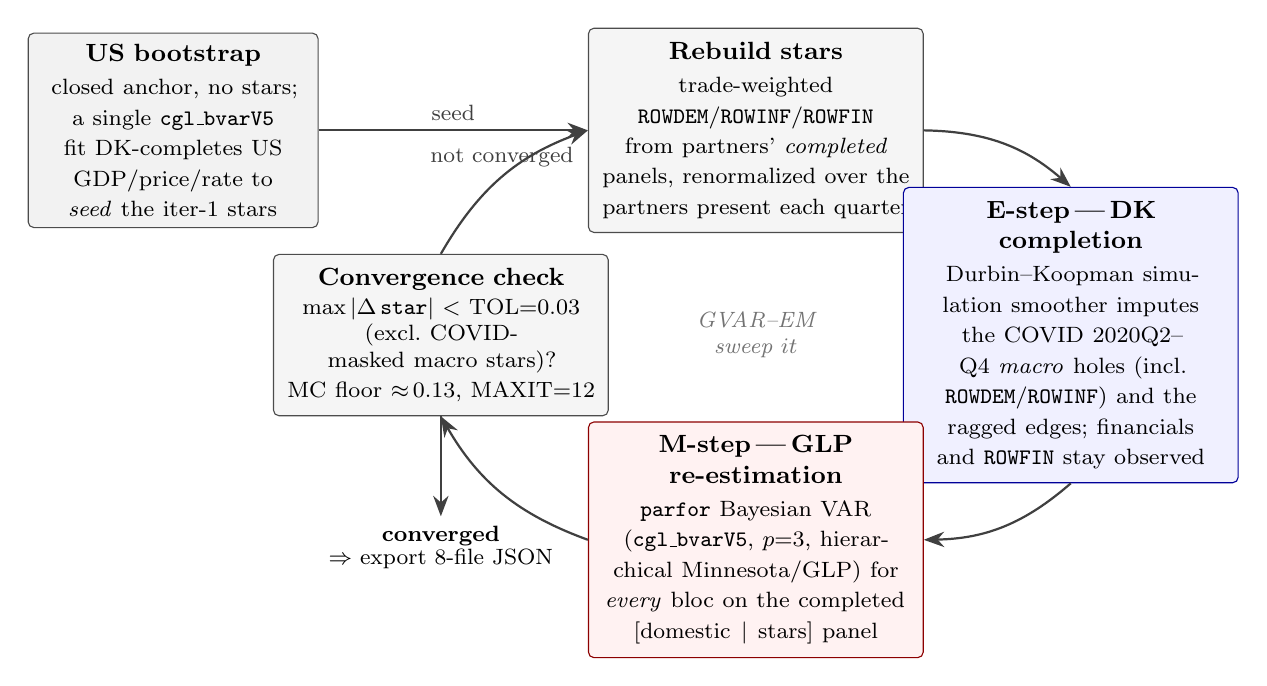
\begin{tikzpicture}[
    >={Stealth[length=2.6mm]},
    font=\small,
    boot/.style={rounded corners=2pt, draw=black!70, fill=black!5,
                 align=center, inner sep=4pt, text width=3.4cm},
    estep/.style={rounded corners=2pt, draw=blue!60!black, fill=blue!6,
                  align=center, inner sep=5pt, text width=3.9cm},
    mstep/.style={rounded corners=2pt, draw=red!55!black, fill=red!5,
                  align=center, inner sep=5pt, text width=3.9cm},
    starbox/.style={rounded corners=2pt, draw=black!70, fill=black!4,
                 align=center, inner sep=5pt, text width=3.9cm},
    convbox/.style={rounded corners=2pt, draw=black!70, fill=black!4,
                 align=center, inner sep=5pt, text width=3.9cm},
    flow/.style={->, thick, black!75},
]
% --- US bootstrap: entry into the loop (seeds the first stars) ---
\node[boot] (boot) at (-7.4,2.6)
  {\textbf{US bootstrap}\\[1pt]
   \footnotesize closed anchor, no stars; a single
   \texttt{cgl\_bvarV5} fit DK-completes US GDP/price/rate to
   \emph{seed} the iter-1 stars};

% --- cycle nodes (clockwise: stars -> E -> M -> conv -> stars) ---
\node[starbox] (stars) at (0,2.6)
  {\textbf{Rebuild stars}\\[1pt]
   \footnotesize trade-weighted \texttt{ROWDEM}/\texttt{ROWINF}/%
   \texttt{ROWFIN} from partners' \emph{completed} panels,
   renormalized over the partners present each quarter};

\node[estep] (estep) at (4.0,0)
  {\textbf{E-step\,---\,DK completion}\\[1pt]
   \footnotesize Durbin--Koopman simulation smoother imputes the
   COVID 2020Q2--Q4 \emph{macro} holes (incl.\ \texttt{ROWDEM}/%
   \texttt{ROWINF}) and the ragged edges; financials and
   \texttt{ROWFIN} stay observed};

\node[mstep] (mstep) at (0,-2.6)
  {\textbf{M-step\,---\,GLP re-estimation}\\[1pt]
   \footnotesize \texttt{parfor} Bayesian VAR (\texttt{cgl\_bvarV5},
   $p{=}3$, hierarchical Minnesota/GLP) for \emph{every} bloc on the
   completed $[\text{domestic}\mid\text{stars}]$ panel};

\node[convbox] (conv) at (-4.0,0)
  {\textbf{Convergence check}\\[1pt]
   \footnotesize $\max|\Delta\,\texttt{star}| < \mathrm{TOL}{=}0.03$
   (excl.\ COVID-masked macro stars)?\\
   MC floor ${\approx}\,0.13$, $\mathrm{MAXIT}{=}12$};

% --- entry arrow ---
\draw[flow] (boot.east) -- node[above,font=\footnotesize]{seed} (stars.west);

% --- the clockwise cycle ---
\draw[flow] (stars.east)  to[bend left=20] (estep.north);
\draw[flow] (estep.south) to[bend left=20] (mstep.east);
\draw[flow] (mstep.west)  to[bend left=20] (conv.south);
\draw[flow] (conv.north)  to[bend left=20]
  node[above,font=\footnotesize]{not converged} (stars.west);

% --- converged exit ---
\node[align=center, font=\footnotesize] (out) at (-4.0,-2.7)
  {\textbf{converged}\\[-1pt]$\Rightarrow$ export 8-file JSON};
\draw[flow] (conv.south) -- (out.north);

% --- loop label ---
\node[font=\footnotesize\itshape, text=black!55, align=center] at (0,0)
  {GVAR--EM\\sweep $it$};
\end{tikzpicture}
\caption{The GVAR-EM estimation loop under pervasive missingness
\citep{GiannoneLenzaPrimiceri2019, DurbinKoopman2002}. A closed US
bootstrap (no stars) is estimated once to seed the first trade-weighted
foreign variables. Each sweep then (i)~rebuilds the
\texttt{ROWDEM}/\texttt{ROWINF}/\texttt{ROWFIN} stars from partners'
completed panels, renormalized over the partners present each quarter,
and (ii)~re-estimates every bloc by hierarchical-prior Bayesian VAR
(Gibbs, run in \texttt{parfor}). Within each bloc's single
\texttt{cgl\_bvarV5} pass the \textbf{E-step}---a Durbin--Koopman
simulation-smoother completion that imputes the COVID macro holes (the
fixed 2020Q2--Q4 window, with financial series and \texttt{ROWFIN} held
observed) and the ragged, unbalanced-panel edges---and the
\textbf{M-step}---the posterior re-estimation of the VAR coefficients on
the completed $[\text{domestic}\mid\text{stars}]$ panel---are carried out
jointly by the same sampler. The sweep repeats until the foreign
components stop moving, $\max|\Delta\,\texttt{star}| < \mathrm{TOL}=0.03$
(evaluated after the second sweep and excluding the COVID-masked macro
stars, whose cross-iteration churn is Monte-Carlo noise with floor
${\approx}\,0.13$), capped at $\mathrm{MAXIT}=12$ iterations.}
\label{fig:em-loop}
\end{figure}

The 2020 pandemic quarters are an extreme outlier that, left untreated,
would contaminate the autoregressive estimates and the innovation
covariance. Rather than scaling them out, the tool treats the pandemic
window as \emph{missing data} and imputes it within the estimation
itself, via a data-augmentation Gibbs sampler that nests a
Durbin--Koopman simulation smoother \citep{DurbinKoopman2002,
DurbinKoopman2012}. Each Gibbs sweep alternates:
\begin{enumerate}[label=(\roman*)]
  \item a Durbin--Koopman simulation-smoother draw of the missing
    pandemic rows given the current coefficients, treating those rows as
    \texttt{NaN} observations in the companion-form state space of
    Section~\ref{sec:statespace};
  \item a Metropolis--Hastings update of the hierarchical-prior
    hyperparameters on the \emph{completed-data} marginal likelihood, so
    the overall tightness $\lambda$ and the sum-of-coefficients
    parameter $\mu$ \citep{Giannone2015} are selected by empirical Bayes
    without any fixed-tightness restriction; and
  \item a draw of the VAR coefficients $(\beta,\Sigma)$ from the
    completed data.
\end{enumerate}
The pandemic history is thus \emph{preserved} (the surrounding quarters
remain in the sample and inform the imputation) while the outlier itself
does not drive the dynamics.

\paragraph{Window selection.} The COVID window self-calibrates to each
bloc's pandemic trough rather than being hard-coded. It is the
\emph{argmin} of the quarter-on-quarter GDP change \emph{restricted to
the window 2019Q4--2021Q1}:
\begin{equation}\label{eq:covid-window}
  k^\star = \operatorname*{arg\,min}_{t \,\in\,\{\text{2019Q4},\dots,\text{2021Q1}\}}
            \bigl(x^{g}_t - x^{g}_{t-1}\bigr),
  \qquad
  \mathcal{W} = \{\,k^\star-1,\ k^\star,\ k^\star+1,\ k^\star+2\,\},
\end{equation}
and the four rows of $\mathcal{W}$ (intersected with the sample) are
NaN'd across \emph{all} variables before estimation. Restricting the
search to 2019Q4--2021Q1 is deliberate: an unrestricted global argmin
misfires for economies whose deepest contraction is a different crisis
(for example Korea's 2008Q4 Global-Financial-Crisis drop exceeds its
2020Q2 pandemic drop).

\paragraph{Fixed window and macro-only masking in the production GVAR
loop.} The auto-detected window above is the legacy single-bloc
convention; the production GVAR estimator
(\texttt{pipeline/export\_bvar\_gvar24\_loop.m}) instead uses a
\emph{fixed} three-quarter window $\mathcal{W}=\{$2020Q2, 2020Q3,
2020Q4$\}$ for every bloc, which avoids the $\sim$seven-quarter spans the
unrestricted trough search could produce. Equally important, the
production loop masks \emph{only the macro columns}: over $\mathcal{W}$
the domestic macro variables (\(\texttt{isFinancial}=\textsf{false}\))
and the two macro stars \texttt{ROWDEM}/\texttt{ROWINF} are set
\texttt{NaN}, while the domestic financial series (rates, yields,
equity, house prices, corporate spreads) and the financial star
\texttt{ROWFIN} are \emph{kept observed}. The Durbin--Koopman smoother
then imputes the pandemic macro holes \emph{conditional on} the observed
financials, which carry genuine signal through 2020---the masking is thus
``macro-masked / financials-observed,'' the same convention the
out-of-sample evaluation re-applies in-sample at every origin
(Section~\ref{sec:empirical:oos}).

Algorithm~\ref{alg:emgvar} states the full estimation loop. It is the
operational form of the cycle sketched in Figure~\ref{fig:em-loop}: a
no-stars US bootstrap seeds the first foreign variables, after which each
sweep rebuilds every bloc's trade-weighted stars from partners' completed
panels (the \emph{E-step} regressor), re-estimates all blocs in parallel
under macro masking (the per-bloc \texttt{cgl\_bvarV5} call, whose own
Durbin--Koopman completion is the within-bloc \emph{E-step} and whose
Gibbs re-estimation is the \emph{M-step}), and recomputes the stars from
the freshly completed data, iterating to a fixed point in the completed
stars.

\begin{algorithm}[!ht]
\caption{EM-style GVAR estimation loop (Jacobi star re-convergence;
\texttt{export\_bvar\_gvar24\_loop.m}).}
\label{alg:emgvar}
\algIn{per-bloc panels $\{X_c\}$ ($X_c=[\text{domestic}\mid\text{stars}]$);
trade weights $W$; lags $p=3$; \texttt{WN}/stationary index sets
$\texttt{pos}_c$; tolerance $\textsc{tol}=0.03$; cap $\textsc{maxit}=12$;
fixed COVID window $\mathcal{W}=\{$2020Q2..Q4$\}$.}
\algOut{per-bloc posterior means $(\hat\beta_c,\hat\Sigma_c)$, completed
panels, predictive draws $\texttt{Dforecast}_c$, exported 8-file JSON.}
\begin{algsteps}
\item \algComment{Bootstrap (seed the first stars).}
\item Mask the US macro columns over $\mathcal{W}$ and fit the closed,
no-stars US bloc with \texttt{cgl\_bvarV5}; the posterior-mean DK
completion gives the initial US real-GDP/price/rate panel
(this seeds partners' iteration-1 stars).
\item \algKw{for} $it = 1,\dots,\textsc{maxit}$ \algKw{do} \algComment{Jacobi sweep}
\item \algInd \algComment{Build all stars from the FROZEN start-of-sweep completed panels.}
\item \algInd \algKw{for each} re-estimated bloc $c$: \texttt{star}$_c \gets$ trade-weighted
\texttt{ROWDEM}/\texttt{ROWINF}/\texttt{ROWFIN} from partners' completed panels (renormalize over partners present each quarter).
\item \algInd \algKw{parfor each} bloc $c$ \algKw{do} \algComment{independent given the frozen stars}
\item \algIndd $x_c \gets [\,\text{domestic}_c \mid \texttt{star}_c\,]$
\item \algIndd over $\mathcal{W}$, set \texttt{NaN} the macro columns of $x_c$ \emph{and} \texttt{ROWDEM},\texttt{ROWINF} (keep financials, \texttt{ROWFIN})
\item \algIndd $(\texttt{Xcond}_c,\beta_c,\Sigma_c,\texttt{Dforecast}_c) \gets \texttt{cgl\_bvarV5}(x_c,\,p,\,\texttt{pos}_c,\dots)$ \algComment{E-step DK completion + M-step Gibbs}
\item \algIndd completed panel $\widehat X_c \gets \operatorname{mean}_{\text{draws}} \texttt{Xcond}_c$
\item \algInd \algKw{end parfor}
\item \algInd $mc \gets \max_{c}\, \max\bigl|\,\texttt{star}_c^{(it)} - \texttt{star}_c^{(it-1)}\,\bigr|$ \algComment{exclude COVID-masked \texttt{ROWDEM}/\texttt{ROWINF} cells}
\item \algInd \algKw{if} $it>1$ \algKw{and} $mc<\textsc{tol}$ \algKw{then break} \algComment{converged}
\item \algKw{end for}
\item Export each bloc's $(\hat\beta_c,\hat\Sigma_c)$, completed history, stars, and predictive draws to the 8-file JSON contract.
\end{algsteps}
\end{algorithm}

The sweep is a \emph{Jacobi} update---all stars are rebuilt from the
common start-of-sweep state \emph{before} the parallel re-estimation---so
the parallel blocs are mutually independent given the current stars and
the sweep has the same fixed point as a sequential (Gauss--Seidel) pass,
at a wall-clock set by the slowest single bloc (the $n=41$ US bloc)
rather than the sum. The convergence metric excludes the COVID-masked
macro-star cells, whose cross-sweep churn is pure imputation Monte-Carlo
noise (floor $\approx 0.13$); the financial star \texttt{ROWFIN}, kept
observed through the pandemic, stays in the metric. Each
\texttt{cgl\_bvarV5} call is itself the data-augmentation Gibbs sampler of
Algorithm~\ref{alg:dksmoother}---its DK completion is the bloc-level
E-step and its hyperparameter/coefficient draws are the M-step---so the
whole loop is a block-coordinate EM over (foreign stars,
completed-data states, VAR coefficients).

\subsection{Common-Vintage Harmonization and the 2026Q1 Observed
Refresh}\label{sec:vintage}

The shipped panels are the product of two distinct, clearly-separated
steps: an \emph{estimation-build harmonization} to a common 2025Q4
endpoint (the vintage every bloc's coefficients were estimated on), and a
later \emph{no-re-estimation observed-data refresh} that advances the
\emph{observed} panel one quarter to 2026Q1 without touching the frozen
estimates. The two are described in turn.

\paragraph{Step 1 --- estimation-build harmonization to 2025Q4.} So that
estimation runs on a uniform window, every bloc's domestic series was
first extended to a common 2025Q4 endpoint by the GVAR build
(\texttt{pipeline/build\_gvar\_2025q4.py}, \texttt{TARGET\_END}${}={}$%
2025Q4). For blocs whose quarterly data ended short of 2025Q4:
\begin{itemize}
  \item \textbf{Real-activity and price series} (GDP, consumption,
    investment, government, exports, imports, CPI/HICP, all \texttt{log})
    are benchmarked to IMF World Economic Outlook annual projections
    (\texttt{NGDP\_RPCH} real growth, \texttt{PCPIPCH} inflation) via
    temporal disaggregation: a within-year quarterly profile is laid
    down at the WEO-implied annual growth and then proportional-Denton
    corrected so that each fully appended year's four-quarter average
    reproduces the WEO annual level (already-observed quarters in a
    partial year are held fixed). The realized annual growth of each
    appended year matches WEO to within $0.2$pp.
  \item \textbf{Financial series with no WEO analogue} (NEER, REER,
    equity indices, and all \texttt{lin} rates --- short rates, 3-month
    rates, 10-year yields, unemployment) are carried forward by
    \emph{hold-last} and flagged as such.
\end{itemize}
The original raw vintages are left untouched; the extended panels are
written separately and consumed by the estimation drivers. The estimated
companion, posterior draws, coupling artifact, and trade weights are all
frozen as of this 2025Q4 build.

\paragraph{Step 2 --- the 2026Q1 observed-data refresh (no
re-estimation).} The live panel then advances one quarter to a default
last-historical of \textbf{2026Q1}, making 2026Q2 the first projected
quarter for the refreshed blocs. This is a pure data extension performed
by \texttt{app/scripts/refresh-quarter.mjs}: for each refreshed bloc the
single new 2026Q1 row is pulled from the \emph{same} live sources, in the
\emph{same} transform, that produced the prior 2025Q4 row, and the
forecast simply re-anchors from the \emph{unchanged} companion. No
estimation runs --- \texttt{cgl\_bvarV5.m} is never invoked, and
\texttt{companion\_mean}, \texttt{companion\_draws}, \texttt{spec},
\texttt{transformations}, \texttt{coupling}, and \texttt{weights} stay
byte-frozen. The script is fail-closed: a bloc is advanced only once a
verified live-source registry (\texttt{SOURCES[<CC>]}) has been authored
and gated for it, so the rollout is per-bloc rather than a single sweep.

\paragraph{The ragged edge (panel default 2026Q1; three exceptions).}
The default last-historical quarter is \textbf{2026Q1}; three blocs are
held earlier because their genuine source data have not advanced and are
\emph{never} fabricated forward (the no-fabrication rule of
Section~\ref{sec:covid}):
\begin{itemize}
  \item \textbf{China (\texttt{CN}) and India (\texttt{IN})} --- held at
    \textbf{2025Q4}. Their real source data still end $\approx$2025Q2, so
    their 2025Q4 tail is the WEO temporal-disaggregation back-fill of
    Step~1 and they are deliberately \emph{not} advanced to 2026Q1.
  \item \textbf{Israel (\texttt{IL})} --- held at \textbf{2024Q4}, its
    quarterly source not yet having advanced.
\end{itemize}
These per-bloc endpoints are pinned in \texttt{app/src/lib/dates.ts}
(\texttt{DEFAULT\_LAST\_HIST\_DATE}${}={}$2026Q1 with \texttt{CN}/%
\texttt{IN}/\texttt{IL} overrides) so the ragged edge plots correctly:
each bloc's first forecast quarter is the one immediately after its own
last observation. A small number of emerging-market blocs
(\texttt{KR}, \texttt{RU}, \texttt{ID}, \texttt{TH}) carry a short trailing
tail whose genuine-versus-synthetic provenance is flagged for review in
Section~\ref{sec:datasources}.

\subsection{Predictive Uncertainty Bands}\label{sec:bands}

For every bloc the exported baseline carries \emph{predictive} bands,
not parameter-only bands. The COVID-missing Gibbs sampler emits a
forecast density that integrates over three sources of uncertainty
simultaneously --- posterior parameter uncertainty, future innovation
uncertainty, and missing-data (imputation) uncertainty. The reported
quantiles are the $5$th, $16$th, $84$th, and $95$th percentiles of this
predictive density (with the $50$th retained in level space),
\begin{equation}\label{eq:bands}
  \bigl(q_{05},\,q_{16},\,q_{84},\,q_{95}\bigr)_{T+h}
  = \mathrm{Quantile}_{\{0.05,0.16,0.84,0.95\}}
    \bigl\{\, \tilde{y}^{(d)}_{T+h} \,\bigr\}_{d=1}^{D},
\end{equation}
yielding the $68\%$ band $(q_{16},q_{84})$ shaded in the charts and the
$90\%$ band $(q_{05},q_{95})$. Crucially, the central path
$\bar{y}^{\text{baseline}}$ remains the \emph{deterministic} forecast
from the posterior-mean coefficients (so the unconditional smoother of
Section~\ref{sec:delta} reproduces it exactly, and zero user deviations
return the stored baseline); only the bands are predictive. This is the
designed fix for the previously over-tight bands that resulted from
spreading posterior-mean paths under a tight prior --- wide bands now
reflect genuine macro volatility (e.g.\ CN, JP, UK), not the COVID
outlier. On-the-fly conditional bands computed in the browser use the
same predictive construction, drawing innovations through the simulation
smoother of Section~\ref{sec:uncertainty}.

\subsection{US Specification}\label{sec:us-spec}

The US is the largest bloc, with $n=41$ quarterly variables and $p=3$ lags.
Its full variable list is given in Table~\ref{tab:vars}; the four-variable
fiscal block (\texttt{FREV\_GDP}, \texttt{FPEXP\_GDP}, \texttt{EFFI},
\texttt{SFA}) supports scenario conditioning on the fiscal drivers and the
debt-targeting inversion (the debt-anchor motivation being the fiscal
reaction function of \citealp{Bohn1998}, though no $\gamma$ feedback is
active in the live recursion; see \S\ref{sec:fiscal_levers}), and the
conditional-forecast and optimal-policy machinery of
\citet{BanburaGiannoneLenza2015} and \citet{BarnichonMesters2023}
applies uniformly across all blocs. The count of $41$ comprises the domestic and
fiscal variables, the four global commons, and the three trade-weighted
\texttt{ROW*\_US} star variables that make the US a fully coupled GVAR bloc
(Section~\ref{sec:gvar:arch}).

\begin{longtable}{lp{6.5cm}cc}
\caption{Variable coverage for the US BVAR model.  ``Trans.''\ denotes
the data transformation: \texttt{log} = log levels (growth rates
displayed), \texttt{lin} = levels.  ``Prior'' denotes the prior mean:
RW = random walk, WN = white noise.}\label{tab:vars} \\
\toprule
\textbf{ID} & \textbf{Description} & \textbf{Trans.} & \textbf{Prior} \\
\midrule
\endfirsthead
\toprule
\textbf{ID} & \textbf{Description} & \textbf{Trans.} & \textbf{Prior} \\
\midrule
\endhead
\bottomrule
\endfoot
GDPH      & Real Gross Domestic Product & log & RW \\
CH        & Real Personal Consumption Expenditures & log & RW \\
FRH       & Real Private Residential Fixed Investment (nom/deflator) & log & RW \\
FNH       & Real Private Nonresidential Fixed Investment (nom/deflator) & log & RW \\
XH        & Real Exports of Goods \& Services & log & RW \\
MH        & Real Imports of Goods \& Services & log & RW \\
GH        & Real Government Consumption Expenditures \& Gross Investment & log & RW \\
JGDP      & Gross Domestic Product: Chain Price Index & log & RW \\
JC        & Personal Consumption Expenditures: Chain Price Index & log & RW \\
JCXFE     & PCE less Food \& Energy: Chain Price Index & log & RW \\
UI        & CPI-U: All Items & log & RW \\
UIXFDG    & CPI-U: All Items Less Food \& Energy & log & RW \\
LXBC      & Business Sector: Compensation Per Hour (nominal) & log & RW \\
LANAGRA   & All Employees: Total Nonfarm & log & RW \\
LR        & Civilian Unemployment Rate: 16 yr + & lin & RW \\
IP        & Industrial Production Index & log & RW \\
CUMFG     & Capacity Utilization: Manufacturing [SIC] & lin & RW \\
HST       & Housing Starts & log & RW \\
YPDH      & Real Disposable Personal Income & log & RW \\
CSENT     & University of Michigan: Consumer Sentiment & lin & RW \\
POLRATE   & Effective Federal Funds Rate (policy rate) & lin & RW \\
FCM2      & 2-Year Treasury Note Yield at Constant Maturity & lin & RW \\
FCM5      & 5-Year Treasury Note Yield at Constant Maturity & lin & RW \\
GLB\_USLR & US 10-Year Treasury Yield (global common) & lin & RW \\
FAAA      & Moodys Seasoned Aaa Corporate Bond Yield & lin & RW \\
GLB\_USBAA& US Baa Corporate Bond Yield, credit proxy (global common) & lin & RW \\
FXTWM     & Nominal Trade-Weighted Exch Value of US\$ vs AFE Currencies & log & RW \\
GLB\_USEQ & US Equity Price Index (global common) & log & RW \\
PZTEXP    & Spot Oil Price: West Texas Intermediate & log & RW \\
GSNE      & Non-Fuel Commodity Price Index (IMF, non-energy proxy) & log & RW \\
SP500VOL  & CBOE Volatility Index for S\&P 500 Stock Price Index & lin & RW \\
HP        & House Price & log & RW \\
LEV       & Real nonfinancial business debt & log & RW \\
FREV\_GDP & Federal Receipts (\% of GDP) & lin & WN \\
FPEXP\_GDP& Federal Primary Expenditure (\% of GDP) & lin & WN \\
EFFI      & Federal Effective Interest Rate (\% p.a.) & lin & RW \\
SFA       & Stock-Flow Adjustment (\% of GDP) & lin & WN \\
GLB\_OIL  & Spot Oil Price, WTI (global common) & log & RW \\
ROWDEM\_US& US RoW demand (trade-weighted partner GDP growth) & lin & RW \\
ROWINF\_US& US RoW inflation (trade-weighted partner inflation) & lin & RW \\
ROWFIN\_US& US RoW financial conditions (trade-weighted partner rates) & lin & RW \\
\end{longtable}

The other coupled blocs follow the same estimation methodology with
country-appropriate variable selections, replacing the US fiscal and
detailed financial block with the three \texttt{ROW*} stars of
Section~\ref{sec:gvar-roster}. Across the deployed roster the partner
blocs range from $n=14$ (Costa Rica) to $n=25$ (UK and Canada), with the
euro-area aggregate at $n=24$ and the core majors at $n\in\{18,\dots,25\}$
(e.g.\ CH, NO~$=18$, CN~$=20$, JP~$=23$); the US is the largest at $n=41$.
The China bloc uses a tighter Minnesota tightness to discipline its
shorter, noisier sample.

\subsection{Variable Transformations, Priors, and Financial Tags by Economy}\label{sec:varcoherence}

Section~\ref{sec:us-spec} tabulates the US bloc in full; this subsection
extends that detail to \emph{every} deployed economy. For all $50$ blocs
(the $33$ GVAR members of Section~\ref{sec:gvar-roster} and the $17$
euro-area standalones of Section~\ref{sec:standalone}) each variable's
\emph{transformation} (\texttt{log} = log level, growth displayed;
\texttt{lin} = level), its \emph{financial} tag (which governs whether a
series is held observed through the COVID window, Section~\ref{sec:covid}),
and its \emph{prior} mean (RW = random walk in levels; WN = white noise /
stationary) are read directly from the deployed
\texttt{public/data/bvar/<CC>/spec.json} specifications, so the tables below
mirror the current re-estimated state of the tool exactly.

\paragraph{Cross-economy coherence matrix.} Table~\ref{tab:coherence}
collects the common concepts that recur across blocs. Because the
transformation, financial tag, and prior for each concept are assigned
\emph{identically} in every economy that carries it, a single row
characterises the concept tool-wide. Every variable is given a
random-walk (RW) prior \emph{except} the three fiscal GDP-ratios
(\texttt{FREV\_GDP}, \texttt{FPEXP\_GDP}, \texttt{SFA}), which are bounded
mean-reverting shares and therefore carry a white-noise / stationary (WN)
prior; the effective-interest series \texttt{EFFI} remains RW.

\begin{table}[!ht]
\centering\small
\caption{Cross-economy coherence matrix for the common concepts. ``Trans.''
is \texttt{log}/\texttt{lin}; ``Fin.''\ marks financial series
($\checkmark$); ``Prior''\ is RW (random walk) or WN (white noise /
stationary). Each concept takes the same triple in every bloc that carries
it.}\label{tab:coherence}
\begin{tabular}{lccc}
\toprule
\textbf{Concept} & \textbf{Trans.} & \textbf{Fin.} & \textbf{Prior} \\
\midrule
Real GDP (level) & \texttt{log} & -- & RW \\
Price index (CPI/HICP/deflator) & \texttt{log} & -- & RW \\
Policy rate & \texttt{lin} & \checkmark & RW \\
Short rate (3M/money-mkt) & \texttt{lin} & \checkmark & RW \\
10Y government yield & \texttt{lin} & \checkmark & RW \\
Corporate / Baa spread & \texttt{lin} & \checkmark & RW \\
House prices & \texttt{log} & \checkmark & RW \\
Equity price index & \texttt{log} & \checkmark & RW \\
Oil price (WTI, global) & \texttt{log} & \checkmark & RW \\
FX / NEER & \texttt{log} & \checkmark & RW \\
Fiscal revenue ratio (FREV\_GDP) & \texttt{lin} & -- & WN \\
Fiscal primary-exp.\ ratio (FPEXP\_GDP) & \texttt{lin} & -- & WN \\
Stock-flow adjustment (SFA) & \texttt{lin} & -- & WN \\
Effective interest (EFFI) & \texttt{lin} & \checkmark & RW \\
RoW demand star (ROWDEM) & \texttt{lin} & \checkmark & RW \\
RoW inflation star (ROWINF) & \texttt{lin} & \checkmark & RW \\
RoW financial star (ROWFIN) & \texttt{lin} & \checkmark & RW \\
\bottomrule
\end{tabular}
\end{table}

\paragraph{The 33 GVAR blocs.} Each carries a domestic block, the four
global commons (\texttt{GLB\_*}), and the three trade-weighted
\texttt{ROW*\_<CC>} stars. Tables follow in alphabetical order.

{\footnotesize
\begin{longtable}{llcc}
\caption{Argentina (\texttt{AR}, $n=18$): variable transformations,
financial tags, and priors.}\label{tab:spec:AR} \\
\toprule
\textbf{ID} & \textbf{Trans.} & \textbf{Fin.} & \textbf{Prior} \\
\midrule
\endfirsthead
\multicolumn{4}{l}{\small\itshape Argentina (\texttt{AR}), continued}\\
\toprule
\textbf{ID} & \textbf{Trans.} & \textbf{Fin.} & \textbf{Prior} \\
\midrule
\endhead
\bottomrule
\endfoot
\texttt{GDP\_AR} & \texttt{log} & -- & RW \\
\texttt{CONS\_AR} & \texttt{log} & -- & RW \\
\texttt{INV\_AR} & \texttt{log} & -- & RW \\
\texttt{GOV\_AR} & \texttt{log} & -- & RW \\
\texttt{EXP\_AR} & \texttt{log} & -- & RW \\
\texttt{IMP\_AR} & \texttt{log} & -- & RW \\
\texttt{CPI\_AR} & \texttt{log} & -- & RW \\
\texttt{LR\_AR} & \texttt{lin} & -- & RW \\
\texttt{RATE\_AR} & \texttt{lin} & \checkmark & RW \\
\texttt{NEER\_AR} & \texttt{log} & \checkmark & RW \\
\texttt{POLRATE\_AR} & \texttt{lin} & \checkmark & RW \\
\texttt{GLB\_OIL} & \texttt{log} & \checkmark & RW \\
\texttt{GLB\_USLR} & \texttt{lin} & \checkmark & RW \\
\texttt{GLB\_USBAA} & \texttt{lin} & \checkmark & RW \\
\texttt{GLB\_USEQ} & \texttt{log} & \checkmark & RW \\
\texttt{ROWDEM\_AR} & \texttt{lin} & \checkmark & RW \\
\texttt{ROWINF\_AR} & \texttt{lin} & \checkmark & RW \\
\texttt{ROWFIN\_AR} & \texttt{lin} & \checkmark & RW \\
\end{longtable}
\begin{longtable}{llcc}
\caption{Australia (\texttt{AU}, $n=19$): variable transformations,
financial tags, and priors.}\label{tab:spec:AU} \\
\toprule
\textbf{ID} & \textbf{Trans.} & \textbf{Fin.} & \textbf{Prior} \\
\midrule
\endfirsthead
\multicolumn{4}{l}{\small\itshape Australia (\texttt{AU}), continued}\\
\toprule
\textbf{ID} & \textbf{Trans.} & \textbf{Fin.} & \textbf{Prior} \\
\midrule
\endhead
\bottomrule
\endfoot
\texttt{GDP\_AU} & \texttt{log} & -- & RW \\
\texttt{CONS\_AU} & \texttt{log} & -- & RW \\
\texttt{GOV\_AU} & \texttt{log} & -- & RW \\
\texttt{INV\_AU} & \texttt{log} & -- & RW \\
\texttt{EXP\_AU} & \texttt{log} & -- & RW \\
\texttt{IMP\_AU} & \texttt{log} & -- & RW \\
\texttt{CPI\_AU} & \texttt{log} & -- & RW \\
\texttt{LR\_AU} & \texttt{lin} & -- & RW \\
\texttt{NEER\_AU} & \texttt{log} & \checkmark & RW \\
\texttt{RATE\_AU} & \texttt{lin} & \checkmark & RW \\
\texttt{YIELD10\_AU} & \texttt{lin} & \checkmark & RW \\
\texttt{HP\_AU} & \texttt{log} & \checkmark & RW \\
\texttt{GLB\_OIL} & \texttt{log} & \checkmark & RW \\
\texttt{GLB\_USLR} & \texttt{lin} & \checkmark & RW \\
\texttt{GLB\_USBAA} & \texttt{lin} & \checkmark & RW \\
\texttt{GLB\_USEQ} & \texttt{log} & \checkmark & RW \\
\texttt{ROWDEM\_AU} & \texttt{lin} & \checkmark & RW \\
\texttt{ROWINF\_AU} & \texttt{lin} & \checkmark & RW \\
\texttt{ROWFIN\_AU} & \texttt{lin} & \checkmark & RW \\
\end{longtable}
\begin{longtable}{llcc}
\caption{Brazil (\texttt{BR}, $n=18$): variable transformations,
financial tags, and priors.}\label{tab:spec:BR} \\
\toprule
\textbf{ID} & \textbf{Trans.} & \textbf{Fin.} & \textbf{Prior} \\
\midrule
\endfirsthead
\multicolumn{4}{l}{\small\itshape Brazil (\texttt{BR}), continued}\\
\toprule
\textbf{ID} & \textbf{Trans.} & \textbf{Fin.} & \textbf{Prior} \\
\midrule
\endhead
\bottomrule
\endfoot
\texttt{GDP\_BR} & \texttt{log} & -- & RW \\
\texttt{CONS\_BR} & \texttt{log} & -- & RW \\
\texttt{INV\_BR} & \texttt{log} & -- & RW \\
\texttt{GOV\_BR} & \texttt{log} & -- & RW \\
\texttt{EXP\_BR} & \texttt{log} & -- & RW \\
\texttt{IMP\_BR} & \texttt{log} & -- & RW \\
\texttt{CPI\_BR} & \texttt{log} & -- & RW \\
\texttt{LR\_BR} & \texttt{lin} & -- & RW \\
\texttt{NEER\_BR} & \texttt{log} & \checkmark & RW \\
\texttt{POLRATE\_BR} & \texttt{lin} & \checkmark & RW \\
\texttt{HP\_BR} & \texttt{log} & \checkmark & RW \\
\texttt{GLB\_OIL} & \texttt{log} & \checkmark & RW \\
\texttt{GLB\_USLR} & \texttt{lin} & \checkmark & RW \\
\texttt{GLB\_USBAA} & \texttt{lin} & \checkmark & RW \\
\texttt{GLB\_USEQ} & \texttt{log} & \checkmark & RW \\
\texttt{ROWDEM\_BR} & \texttt{lin} & \checkmark & RW \\
\texttt{ROWINF\_BR} & \texttt{lin} & \checkmark & RW \\
\texttt{ROWFIN\_BR} & \texttt{lin} & \checkmark & RW \\
\end{longtable}
\begin{longtable}{llcc}
\caption{Canada (\texttt{CA}, $n=25$): variable transformations,
financial tags, and priors.}\label{tab:spec:CA} \\
\toprule
\textbf{ID} & \textbf{Trans.} & \textbf{Fin.} & \textbf{Prior} \\
\midrule
\endfirsthead
\multicolumn{4}{l}{\small\itshape Canada (\texttt{CA}), continued}\\
\toprule
\textbf{ID} & \textbf{Trans.} & \textbf{Fin.} & \textbf{Prior} \\
\midrule
\endhead
\bottomrule
\endfoot
\texttt{GDP\_CA} & \texttt{log} & -- & RW \\
\texttt{CONS\_CA} & \texttt{log} & -- & RW \\
\texttt{INV\_CA} & \texttt{log} & -- & RW \\
\texttt{GOV\_CA} & \texttt{log} & -- & RW \\
\texttt{EXP\_CA} & \texttt{log} & -- & RW \\
\texttt{IMP\_CA} & \texttt{log} & -- & RW \\
\texttt{IP\_CA} & \texttt{log} & -- & RW \\
\texttt{LR\_CA} & \texttt{lin} & -- & RW \\
\texttt{CPI\_CA} & \texttt{log} & -- & RW \\
\texttt{RATE\_CA} & \texttt{lin} & \checkmark & RW \\
\texttt{POLRATE\_CA} & \texttt{lin} & \checkmark & RW \\
\texttt{YIELD10\_CA} & \texttt{lin} & \checkmark & RW \\
\texttt{HP\_CA} & \texttt{log} & \checkmark & RW \\
\texttt{NEER\_CA} & \texttt{log} & \checkmark & RW \\
\texttt{GLB\_OIL} & \texttt{log} & \checkmark & RW \\
\texttt{GLB\_USLR} & \texttt{lin} & \checkmark & RW \\
\texttt{GLB\_USBAA} & \texttt{lin} & \checkmark & RW \\
\texttt{GLB\_USEQ} & \texttt{log} & \checkmark & RW \\
\texttt{FREV\_GDP} & \texttt{lin} & -- & WN \\
\texttt{FPEXP\_GDP} & \texttt{lin} & -- & WN \\
\texttt{EFFI} & \texttt{lin} & \checkmark & RW \\
\texttt{SFA} & \texttt{lin} & -- & WN \\
\texttt{ROWDEM\_CA} & \texttt{lin} & \checkmark & RW \\
\texttt{ROWINF\_CA} & \texttt{lin} & \checkmark & RW \\
\texttt{ROWFIN\_CA} & \texttt{lin} & \checkmark & RW \\
\end{longtable}
\begin{longtable}{llcc}
\caption{Switzerland (\texttt{CH}, $n=18$): variable transformations,
financial tags, and priors.}\label{tab:spec:CH} \\
\toprule
\textbf{ID} & \textbf{Trans.} & \textbf{Fin.} & \textbf{Prior} \\
\midrule
\endfirsthead
\multicolumn{4}{l}{\small\itshape Switzerland (\texttt{CH}), continued}\\
\toprule
\textbf{ID} & \textbf{Trans.} & \textbf{Fin.} & \textbf{Prior} \\
\midrule
\endhead
\bottomrule
\endfoot
\texttt{GDP\_CH} & \texttt{log} & -- & RW \\
\texttt{CONS\_CH} & \texttt{log} & -- & RW \\
\texttt{INV\_CH} & \texttt{log} & -- & RW \\
\texttt{GOV\_CH} & \texttt{log} & -- & RW \\
\texttt{EXP\_CH} & \texttt{log} & -- & RW \\
\texttt{IMP\_CH} & \texttt{log} & -- & RW \\
\texttt{HICP\_CH} & \texttt{log} & -- & RW \\
\texttt{LR\_CH} & \texttt{lin} & -- & RW \\
\texttt{NEER\_CH} & \texttt{log} & \checkmark & RW \\
\texttt{POLRATE\_CH} & \texttt{lin} & \checkmark & RW \\
\texttt{HP\_CH} & \texttt{log} & \checkmark & RW \\
\texttt{GLB\_OIL} & \texttt{log} & \checkmark & RW \\
\texttt{GLB\_USLR} & \texttt{lin} & \checkmark & RW \\
\texttt{GLB\_USBAA} & \texttt{lin} & \checkmark & RW \\
\texttt{GLB\_USEQ} & \texttt{log} & \checkmark & RW \\
\texttt{ROWDEM\_CH} & \texttt{lin} & \checkmark & RW \\
\texttt{ROWINF\_CH} & \texttt{lin} & \checkmark & RW \\
\texttt{ROWFIN\_CH} & \texttt{lin} & \checkmark & RW \\
\end{longtable}
\begin{longtable}{llcc}
\caption{Chile (\texttt{CL}, $n=20$): variable transformations,
financial tags, and priors.}\label{tab:spec:CL} \\
\toprule
\textbf{ID} & \textbf{Trans.} & \textbf{Fin.} & \textbf{Prior} \\
\midrule
\endfirsthead
\multicolumn{4}{l}{\small\itshape Chile (\texttt{CL}), continued}\\
\toprule
\textbf{ID} & \textbf{Trans.} & \textbf{Fin.} & \textbf{Prior} \\
\midrule
\endhead
\bottomrule
\endfoot
\texttt{GDP\_CL} & \texttt{log} & -- & RW \\
\texttt{CONS\_CL} & \texttt{log} & -- & RW \\
\texttt{INV\_CL} & \texttt{log} & -- & RW \\
\texttt{GOV\_CL} & \texttt{log} & -- & RW \\
\texttt{EXP\_CL} & \texttt{log} & -- & RW \\
\texttt{IMP\_CL} & \texttt{log} & -- & RW \\
\texttt{CPI\_CL} & \texttt{log} & -- & RW \\
\texttt{LR\_CL} & \texttt{lin} & -- & RW \\
\texttt{RATE\_CL} & \texttt{lin} & \checkmark & RW \\
\texttt{POLRATE\_CL} & \texttt{lin} & \checkmark & RW \\
\texttt{YIELD10\_CL} & \texttt{lin} & \checkmark & RW \\
\texttt{HP\_CL} & \texttt{log} & \checkmark & RW \\
\texttt{NEER\_CL} & \texttt{log} & \checkmark & RW \\
\texttt{GLB\_OIL} & \texttt{log} & \checkmark & RW \\
\texttt{GLB\_USLR} & \texttt{lin} & \checkmark & RW \\
\texttt{GLB\_USBAA} & \texttt{lin} & \checkmark & RW \\
\texttt{GLB\_USEQ} & \texttt{log} & \checkmark & RW \\
\texttt{ROWDEM\_CL} & \texttt{lin} & \checkmark & RW \\
\texttt{ROWINF\_CL} & \texttt{lin} & \checkmark & RW \\
\texttt{ROWFIN\_CL} & \texttt{lin} & \checkmark & RW \\
\end{longtable}
\begin{longtable}{llcc}
\caption{China (\texttt{CN}, $n=20$): variable transformations,
financial tags, and priors.}\label{tab:spec:CN} \\
\toprule
\textbf{ID} & \textbf{Trans.} & \textbf{Fin.} & \textbf{Prior} \\
\midrule
\endfirsthead
\multicolumn{4}{l}{\small\itshape China (\texttt{CN}), continued}\\
\toprule
\textbf{ID} & \textbf{Trans.} & \textbf{Fin.} & \textbf{Prior} \\
\midrule
\endhead
\bottomrule
\endfoot
\texttt{GDP\_CN} & \texttt{log} & -- & RW \\
\texttt{CPI\_CN} & \texttt{log} & -- & RW \\
\texttt{RATE\_CN} & \texttt{lin} & \checkmark & RW \\
\texttt{EXP\_CN} & \texttt{log} & -- & RW \\
\texttt{IMP\_CN} & \texttt{log} & -- & RW \\
\texttt{REER\_CN} & \texttt{log} & \checkmark & RW \\
\texttt{EQ\_CN} & \texttt{log} & \checkmark & RW \\
\texttt{POLRATE\_CN} & \texttt{lin} & \checkmark & RW \\
\texttt{HP\_CN} & \texttt{log} & \checkmark & RW \\
\texttt{GLB\_OIL} & \texttt{log} & \checkmark & RW \\
\texttt{GLB\_USLR} & \texttt{lin} & \checkmark & RW \\
\texttt{GLB\_USBAA} & \texttt{lin} & \checkmark & RW \\
\texttt{GLB\_USEQ} & \texttt{log} & \checkmark & RW \\
\texttt{FREV\_GDP} & \texttt{lin} & -- & WN \\
\texttt{FPEXP\_GDP} & \texttt{lin} & -- & WN \\
\texttt{EFFI} & \texttt{lin} & \checkmark & RW \\
\texttt{SFA} & \texttt{lin} & -- & WN \\
\texttt{ROWDEM\_CN} & \texttt{lin} & \checkmark & RW \\
\texttt{ROWINF\_CN} & \texttt{lin} & \checkmark & RW \\
\texttt{ROWFIN\_CN} & \texttt{lin} & \checkmark & RW \\
\end{longtable}
\begin{longtable}{llcc}
\caption{Colombia (\texttt{CO}, $n=20$): variable transformations,
financial tags, and priors.}\label{tab:spec:CO} \\
\toprule
\textbf{ID} & \textbf{Trans.} & \textbf{Fin.} & \textbf{Prior} \\
\midrule
\endfirsthead
\multicolumn{4}{l}{\small\itshape Colombia (\texttt{CO}), continued}\\
\toprule
\textbf{ID} & \textbf{Trans.} & \textbf{Fin.} & \textbf{Prior} \\
\midrule
\endhead
\bottomrule
\endfoot
\texttt{GDP\_CO} & \texttt{log} & -- & RW \\
\texttt{CONS\_CO} & \texttt{log} & -- & RW \\
\texttt{INV\_CO} & \texttt{log} & -- & RW \\
\texttt{GOV\_CO} & \texttt{log} & -- & RW \\
\texttt{EXP\_CO} & \texttt{log} & -- & RW \\
\texttt{IMP\_CO} & \texttt{log} & -- & RW \\
\texttt{CPI\_CO} & \texttt{log} & -- & RW \\
\texttt{LR\_CO} & \texttt{lin} & -- & RW \\
\texttt{RATE\_CO} & \texttt{lin} & \checkmark & RW \\
\texttt{POLRATE\_CO} & \texttt{lin} & \checkmark & RW \\
\texttt{YIELD10\_CO} & \texttt{lin} & \checkmark & RW \\
\texttt{HP\_CO} & \texttt{log} & \checkmark & RW \\
\texttt{NEER\_CO} & \texttt{log} & \checkmark & RW \\
\texttt{GLB\_OIL} & \texttt{log} & \checkmark & RW \\
\texttt{GLB\_USLR} & \texttt{lin} & \checkmark & RW \\
\texttt{GLB\_USBAA} & \texttt{lin} & \checkmark & RW \\
\texttt{GLB\_USEQ} & \texttt{log} & \checkmark & RW \\
\texttt{ROWDEM\_CO} & \texttt{lin} & \checkmark & RW \\
\texttt{ROWINF\_CO} & \texttt{lin} & \checkmark & RW \\
\texttt{ROWFIN\_CO} & \texttt{lin} & \checkmark & RW \\
\end{longtable}
\begin{longtable}{llcc}
\caption{Costa Rica (\texttt{CR}, $n=14$): variable transformations,
financial tags, and priors.}\label{tab:spec:CR} \\
\toprule
\textbf{ID} & \textbf{Trans.} & \textbf{Fin.} & \textbf{Prior} \\
\midrule
\endfirsthead
\multicolumn{4}{l}{\small\itshape Costa Rica (\texttt{CR}), continued}\\
\toprule
\textbf{ID} & \textbf{Trans.} & \textbf{Fin.} & \textbf{Prior} \\
\midrule
\endhead
\bottomrule
\endfoot
\texttt{GDP\_CR} & \texttt{log} & -- & RW \\
\texttt{EXP\_CR} & \texttt{log} & -- & RW \\
\texttt{IMP\_CR} & \texttt{log} & -- & RW \\
\texttt{CPI\_CR} & \texttt{log} & -- & RW \\
\texttt{LR\_CR} & \texttt{lin} & -- & RW \\
\texttt{RATE\_CR} & \texttt{lin} & \checkmark & RW \\
\texttt{NEER\_CR} & \texttt{log} & \checkmark & RW \\
\texttt{GLB\_OIL} & \texttt{log} & \checkmark & RW \\
\texttt{GLB\_USLR} & \texttt{lin} & \checkmark & RW \\
\texttt{GLB\_USBAA} & \texttt{lin} & \checkmark & RW \\
\texttt{GLB\_USEQ} & \texttt{log} & \checkmark & RW \\
\texttt{ROWDEM\_CR} & \texttt{lin} & \checkmark & RW \\
\texttt{ROWINF\_CR} & \texttt{lin} & \checkmark & RW \\
\texttt{ROWFIN\_CR} & \texttt{lin} & \checkmark & RW \\
\end{longtable}
\begin{longtable}{llcc}
\caption{Czechia (\texttt{CZ}, $n=19$): variable transformations,
financial tags, and priors.}\label{tab:spec:CZ} \\
\toprule
\textbf{ID} & \textbf{Trans.} & \textbf{Fin.} & \textbf{Prior} \\
\midrule
\endfirsthead
\multicolumn{4}{l}{\small\itshape Czechia (\texttt{CZ}), continued}\\
\toprule
\textbf{ID} & \textbf{Trans.} & \textbf{Fin.} & \textbf{Prior} \\
\midrule
\endhead
\bottomrule
\endfoot
\texttt{GDP\_CZ} & \texttt{log} & -- & RW \\
\texttt{CONS\_CZ} & \texttt{log} & -- & RW \\
\texttt{INV\_CZ} & \texttt{log} & -- & RW \\
\texttt{GOV\_CZ} & \texttt{log} & -- & RW \\
\texttt{EXP\_CZ} & \texttt{log} & -- & RW \\
\texttt{IMP\_CZ} & \texttt{log} & -- & RW \\
\texttt{HICP\_CZ} & \texttt{log} & -- & RW \\
\texttt{LR\_CZ} & \texttt{lin} & -- & RW \\
\texttt{YIELD10\_CZ} & \texttt{lin} & \checkmark & RW \\
\texttt{NEER\_CZ} & \texttt{log} & \checkmark & RW \\
\texttt{POLRATE\_CZ} & \texttt{lin} & \checkmark & RW \\
\texttt{HP\_CZ} & \texttt{log} & \checkmark & RW \\
\texttt{GLB\_OIL} & \texttt{log} & \checkmark & RW \\
\texttt{GLB\_USLR} & \texttt{lin} & \checkmark & RW \\
\texttt{GLB\_USBAA} & \texttt{lin} & \checkmark & RW \\
\texttt{GLB\_USEQ} & \texttt{log} & \checkmark & RW \\
\texttt{ROWDEM\_CZ} & \texttt{lin} & \checkmark & RW \\
\texttt{ROWINF\_CZ} & \texttt{lin} & \checkmark & RW \\
\texttt{ROWFIN\_CZ} & \texttt{lin} & \checkmark & RW \\
\end{longtable}
\begin{longtable}{llcc}
\caption{Denmark (\texttt{DK}, $n=20$): variable transformations,
financial tags, and priors.}\label{tab:spec:DK} \\
\toprule
\textbf{ID} & \textbf{Trans.} & \textbf{Fin.} & \textbf{Prior} \\
\midrule
\endfirsthead
\multicolumn{4}{l}{\small\itshape Denmark (\texttt{DK}), continued}\\
\toprule
\textbf{ID} & \textbf{Trans.} & \textbf{Fin.} & \textbf{Prior} \\
\midrule
\endhead
\bottomrule
\endfoot
\texttt{GDP\_DK} & \texttt{log} & -- & RW \\
\texttt{CONS\_DK} & \texttt{log} & -- & RW \\
\texttt{INV\_DK} & \texttt{log} & -- & RW \\
\texttt{GOV\_DK} & \texttt{log} & -- & RW \\
\texttt{EXP\_DK} & \texttt{log} & -- & RW \\
\texttt{IMP\_DK} & \texttt{log} & -- & RW \\
\texttt{HICP\_DK} & \texttt{log} & -- & RW \\
\texttt{LR\_DK} & \texttt{lin} & -- & RW \\
\texttt{RATE\_DK} & \texttt{lin} & \checkmark & RW \\
\texttt{YIELD10\_DK} & \texttt{lin} & \checkmark & RW \\
\texttt{NEER\_DK} & \texttt{log} & \checkmark & RW \\
\texttt{POLRATE\_DK} & \texttt{lin} & \checkmark & RW \\
\texttt{HP\_DK} & \texttt{log} & \checkmark & RW \\
\texttt{GLB\_OIL} & \texttt{log} & \checkmark & RW \\
\texttt{GLB\_USLR} & \texttt{lin} & \checkmark & RW \\
\texttt{GLB\_USBAA} & \texttt{lin} & \checkmark & RW \\
\texttt{GLB\_USEQ} & \texttt{log} & \checkmark & RW \\
\texttt{ROWDEM\_DK} & \texttt{lin} & \checkmark & RW \\
\texttt{ROWINF\_DK} & \texttt{lin} & \checkmark & RW \\
\texttt{ROWFIN\_DK} & \texttt{lin} & \checkmark & RW \\
\end{longtable}
\begin{longtable}{llcc}
\caption{Euro Area (\texttt{EA}, $n=24$): variable transformations,
financial tags, and priors.}\label{tab:spec:EA} \\
\toprule
\textbf{ID} & \textbf{Trans.} & \textbf{Fin.} & \textbf{Prior} \\
\midrule
\endfirsthead
\multicolumn{4}{l}{\small\itshape Euro Area (\texttt{EA}), continued}\\
\toprule
\textbf{ID} & \textbf{Trans.} & \textbf{Fin.} & \textbf{Prior} \\
\midrule
\endhead
\bottomrule
\endfoot
\texttt{GDP\_EA} & \texttt{log} & -- & RW \\
\texttt{CONS\_EA} & \texttt{log} & -- & RW \\
\texttt{INV\_EA} & \texttt{log} & -- & RW \\
\texttt{GOV\_EA} & \texttt{log} & -- & RW \\
\texttt{EXP\_EA} & \texttt{log} & -- & RW \\
\texttt{IMP\_EA} & \texttt{log} & -- & RW \\
\texttt{HICP\_EA} & \texttt{log} & -- & RW \\
\texttt{RATE\_EA} & \texttt{lin} & \checkmark & RW \\
\texttt{YIELD10\_EA} & \texttt{lin} & \checkmark & RW \\
\texttt{NEER\_EA} & \texttt{log} & \checkmark & RW \\
\texttt{POLRATE\_EA} & \texttt{lin} & \checkmark & RW \\
\texttt{HPI\_EA} & \texttt{log} & \checkmark & RW \\
\texttt{EACORP} & \texttt{lin} & \checkmark & RW \\
\texttt{GLB\_OIL} & \texttt{log} & \checkmark & RW \\
\texttt{GLB\_USLR} & \texttt{lin} & \checkmark & RW \\
\texttt{GLB\_USBAA} & \texttt{lin} & \checkmark & RW \\
\texttt{GLB\_USEQ} & \texttt{log} & \checkmark & RW \\
\texttt{FREV\_GDP} & \texttt{lin} & -- & WN \\
\texttt{FPEXP\_GDP} & \texttt{lin} & -- & WN \\
\texttt{EFFI} & \texttt{lin} & \checkmark & RW \\
\texttt{SFA} & \texttt{lin} & -- & WN \\
\texttt{ROWDEM\_EA} & \texttt{lin} & \checkmark & RW \\
\texttt{ROWINF\_EA} & \texttt{lin} & \checkmark & RW \\
\texttt{ROWFIN\_EA} & \texttt{lin} & \checkmark & RW \\
\end{longtable}
\begin{longtable}{llcc}
\caption{Hungary (\texttt{HU}, $n=19$): variable transformations,
financial tags, and priors.}\label{tab:spec:HU} \\
\toprule
\textbf{ID} & \textbf{Trans.} & \textbf{Fin.} & \textbf{Prior} \\
\midrule
\endfirsthead
\multicolumn{4}{l}{\small\itshape Hungary (\texttt{HU}), continued}\\
\toprule
\textbf{ID} & \textbf{Trans.} & \textbf{Fin.} & \textbf{Prior} \\
\midrule
\endhead
\bottomrule
\endfoot
\texttt{GDP\_HU} & \texttt{log} & -- & RW \\
\texttt{CONS\_HU} & \texttt{log} & -- & RW \\
\texttt{INV\_HU} & \texttt{log} & -- & RW \\
\texttt{GOV\_HU} & \texttt{log} & -- & RW \\
\texttt{EXP\_HU} & \texttt{log} & -- & RW \\
\texttt{IMP\_HU} & \texttt{log} & -- & RW \\
\texttt{HICP\_HU} & \texttt{log} & -- & RW \\
\texttt{LR\_HU} & \texttt{lin} & -- & RW \\
\texttt{YIELD10\_HU} & \texttt{lin} & \checkmark & RW \\
\texttt{NEER\_HU} & \texttt{log} & \checkmark & RW \\
\texttt{POLRATE\_HU} & \texttt{lin} & \checkmark & RW \\
\texttt{HP\_HU} & \texttt{log} & \checkmark & RW \\
\texttt{GLB\_OIL} & \texttt{log} & \checkmark & RW \\
\texttt{GLB\_USLR} & \texttt{lin} & \checkmark & RW \\
\texttt{GLB\_USBAA} & \texttt{lin} & \checkmark & RW \\
\texttt{GLB\_USEQ} & \texttt{log} & \checkmark & RW \\
\texttt{ROWDEM\_HU} & \texttt{lin} & \checkmark & RW \\
\texttt{ROWINF\_HU} & \texttt{lin} & \checkmark & RW \\
\texttt{ROWFIN\_HU} & \texttt{lin} & \checkmark & RW \\
\end{longtable}
\begin{longtable}{llcc}
\caption{Indonesia (\texttt{ID}, $n=18$): variable transformations,
financial tags, and priors.}\label{tab:spec:ID} \\
\toprule
\textbf{ID} & \textbf{Trans.} & \textbf{Fin.} & \textbf{Prior} \\
\midrule
\endfirsthead
\multicolumn{4}{l}{\small\itshape Indonesia (\texttt{ID}), continued}\\
\toprule
\textbf{ID} & \textbf{Trans.} & \textbf{Fin.} & \textbf{Prior} \\
\midrule
\endhead
\bottomrule
\endfoot
\texttt{GDP\_ID} & \texttt{log} & -- & RW \\
\texttt{CONS\_ID} & \texttt{log} & -- & RW \\
\texttt{INV\_ID} & \texttt{log} & -- & RW \\
\texttt{GOV\_ID} & \texttt{log} & -- & RW \\
\texttt{EXP\_ID} & \texttt{log} & -- & RW \\
\texttt{IMP\_ID} & \texttt{log} & -- & RW \\
\texttt{CPI\_ID} & \texttt{log} & -- & RW \\
\texttt{RATE\_ID} & \texttt{lin} & \checkmark & RW \\
\texttt{NEER\_ID} & \texttt{log} & \checkmark & RW \\
\texttt{POLRATE\_ID} & \texttt{lin} & \checkmark & RW \\
\texttt{HP\_ID} & \texttt{log} & \checkmark & RW \\
\texttt{GLB\_OIL} & \texttt{log} & \checkmark & RW \\
\texttt{GLB\_USLR} & \texttt{lin} & \checkmark & RW \\
\texttt{GLB\_USBAA} & \texttt{lin} & \checkmark & RW \\
\texttt{GLB\_USEQ} & \texttt{log} & \checkmark & RW \\
\texttt{ROWDEM\_ID} & \texttt{lin} & \checkmark & RW \\
\texttt{ROWINF\_ID} & \texttt{lin} & \checkmark & RW \\
\texttt{ROWFIN\_ID} & \texttt{lin} & \checkmark & RW \\
\end{longtable}
\begin{longtable}{llcc}
\caption{Israel (\texttt{IL}, $n=19$): variable transformations,
financial tags, and priors.}\label{tab:spec:IL} \\
\toprule
\textbf{ID} & \textbf{Trans.} & \textbf{Fin.} & \textbf{Prior} \\
\midrule
\endfirsthead
\multicolumn{4}{l}{\small\itshape Israel (\texttt{IL}), continued}\\
\toprule
\textbf{ID} & \textbf{Trans.} & \textbf{Fin.} & \textbf{Prior} \\
\midrule
\endhead
\bottomrule
\endfoot
\texttt{GDP\_IL} & \texttt{log} & -- & RW \\
\texttt{CONS\_IL} & \texttt{log} & -- & RW \\
\texttt{INV\_IL} & \texttt{log} & -- & RW \\
\texttt{GOV\_IL} & \texttt{log} & -- & RW \\
\texttt{EXP\_IL} & \texttt{log} & -- & RW \\
\texttt{IMP\_IL} & \texttt{log} & -- & RW \\
\texttt{CPI\_IL} & \texttt{log} & -- & RW \\
\texttt{LR\_IL} & \texttt{lin} & -- & RW \\
\texttt{RATE\_IL} & \texttt{lin} & \checkmark & RW \\
\texttt{POLRATE\_IL} & \texttt{lin} & \checkmark & RW \\
\texttt{NEER\_IL} & \texttt{log} & \checkmark & RW \\
\texttt{HP\_IL} & \texttt{log} & \checkmark & RW \\
\texttt{GLB\_OIL} & \texttt{log} & \checkmark & RW \\
\texttt{GLB\_USLR} & \texttt{lin} & \checkmark & RW \\
\texttt{GLB\_USBAA} & \texttt{lin} & \checkmark & RW \\
\texttt{GLB\_USEQ} & \texttt{log} & \checkmark & RW \\
\texttt{ROWDEM\_IL} & \texttt{lin} & \checkmark & RW \\
\texttt{ROWINF\_IL} & \texttt{lin} & \checkmark & RW \\
\texttt{ROWFIN\_IL} & \texttt{lin} & \checkmark & RW \\
\end{longtable}
\begin{longtable}{llcc}
\caption{India (\texttt{IN}, $n=20$): variable transformations,
financial tags, and priors.}\label{tab:spec:IN} \\
\toprule
\textbf{ID} & \textbf{Trans.} & \textbf{Fin.} & \textbf{Prior} \\
\midrule
\endfirsthead
\multicolumn{4}{l}{\small\itshape India (\texttt{IN}), continued}\\
\toprule
\textbf{ID} & \textbf{Trans.} & \textbf{Fin.} & \textbf{Prior} \\
\midrule
\endhead
\bottomrule
\endfoot
\texttt{GDP\_IN} & \texttt{log} & -- & RW \\
\texttt{CONS\_IN} & \texttt{log} & -- & RW \\
\texttt{INV\_IN} & \texttt{log} & -- & RW \\
\texttt{GOV\_IN} & \texttt{log} & -- & RW \\
\texttt{EXP\_IN} & \texttt{log} & -- & RW \\
\texttt{IMP\_IN} & \texttt{log} & -- & RW \\
\texttt{CPI\_IN} & \texttt{log} & -- & RW \\
\texttt{RATE\_IN} & \texttt{lin} & \checkmark & RW \\
\texttt{RATE3M\_IN} & \texttt{lin} & \checkmark & RW \\
\texttt{YIELD10\_IN} & \texttt{lin} & \checkmark & RW \\
\texttt{NEER\_IN} & \texttt{log} & \checkmark & RW \\
\texttt{POLRATE\_IN} & \texttt{lin} & \checkmark & RW \\
\texttt{HP\_IN} & \texttt{log} & \checkmark & RW \\
\texttt{GLB\_OIL} & \texttt{log} & \checkmark & RW \\
\texttt{GLB\_USLR} & \texttt{lin} & \checkmark & RW \\
\texttt{GLB\_USBAA} & \texttt{lin} & \checkmark & RW \\
\texttt{GLB\_USEQ} & \texttt{log} & \checkmark & RW \\
\texttt{ROWDEM\_IN} & \texttt{lin} & \checkmark & RW \\
\texttt{ROWINF\_IN} & \texttt{lin} & \checkmark & RW \\
\texttt{ROWFIN\_IN} & \texttt{lin} & \checkmark & RW \\
\end{longtable}
\begin{longtable}{llcc}
\caption{Iceland (\texttt{IS}, $n=19$): variable transformations,
financial tags, and priors.}\label{tab:spec:IS} \\
\toprule
\textbf{ID} & \textbf{Trans.} & \textbf{Fin.} & \textbf{Prior} \\
\midrule
\endfirsthead
\multicolumn{4}{l}{\small\itshape Iceland (\texttt{IS}), continued}\\
\toprule
\textbf{ID} & \textbf{Trans.} & \textbf{Fin.} & \textbf{Prior} \\
\midrule
\endhead
\bottomrule
\endfoot
\texttt{GDP\_IS} & \texttt{log} & -- & RW \\
\texttt{CONS\_IS} & \texttt{log} & -- & RW \\
\texttt{INV\_IS} & \texttt{log} & -- & RW \\
\texttt{GOV\_IS} & \texttt{log} & -- & RW \\
\texttt{EXP\_IS} & \texttt{log} & -- & RW \\
\texttt{IMP\_IS} & \texttt{log} & -- & RW \\
\texttt{CPI\_IS} & \texttt{log} & -- & RW \\
\texttt{LR\_IS} & \texttt{lin} & -- & RW \\
\texttt{RATE\_IS} & \texttt{lin} & \checkmark & RW \\
\texttt{NEER\_IS} & \texttt{log} & \checkmark & RW \\
\texttt{POLRATE\_IS} & \texttt{lin} & \checkmark & RW \\
\texttt{HP\_IS} & \texttt{log} & \checkmark & RW \\
\texttt{GLB\_OIL} & \texttt{log} & \checkmark & RW \\
\texttt{GLB\_USLR} & \texttt{lin} & \checkmark & RW \\
\texttt{GLB\_USBAA} & \texttt{lin} & \checkmark & RW \\
\texttt{GLB\_USEQ} & \texttt{log} & \checkmark & RW \\
\texttt{ROWDEM\_IS} & \texttt{lin} & \checkmark & RW \\
\texttt{ROWINF\_IS} & \texttt{lin} & \checkmark & RW \\
\texttt{ROWFIN\_IS} & \texttt{lin} & \checkmark & RW \\
\end{longtable}
\begin{longtable}{llcc}
\caption{Japan (\texttt{JP}, $n=23$): variable transformations,
financial tags, and priors.}\label{tab:spec:JP} \\
\toprule
\textbf{ID} & \textbf{Trans.} & \textbf{Fin.} & \textbf{Prior} \\
\midrule
\endfirsthead
\multicolumn{4}{l}{\small\itshape Japan (\texttt{JP}), continued}\\
\toprule
\textbf{ID} & \textbf{Trans.} & \textbf{Fin.} & \textbf{Prior} \\
\midrule
\endhead
\bottomrule
\endfoot
\texttt{GDP\_JP} & \texttt{log} & -- & RW \\
\texttt{CONS\_JP} & \texttt{log} & -- & RW \\
\texttt{INV\_JP} & \texttt{log} & -- & RW \\
\texttt{GOV\_JP} & \texttt{log} & -- & RW \\
\texttt{EXP\_JP} & \texttt{log} & -- & RW \\
\texttt{IMP\_JP} & \texttt{log} & -- & RW \\
\texttt{LR\_JP} & \texttt{lin} & -- & RW \\
\texttt{CPI\_JP} & \texttt{log} & -- & RW \\
\texttt{RATE\_JP} & \texttt{lin} & \checkmark & RW \\
\texttt{POLRATE\_JP} & \texttt{lin} & \checkmark & RW \\
\texttt{YIELD10\_JP} & \texttt{lin} & \checkmark & RW \\
\texttt{HP\_JP} & \texttt{log} & \checkmark & RW \\
\texttt{GLB\_OIL} & \texttt{log} & \checkmark & RW \\
\texttt{GLB\_USLR} & \texttt{lin} & \checkmark & RW \\
\texttt{GLB\_USBAA} & \texttt{lin} & \checkmark & RW \\
\texttt{GLB\_USEQ} & \texttt{log} & \checkmark & RW \\
\texttt{FREV\_GDP} & \texttt{lin} & -- & WN \\
\texttt{FPEXP\_GDP} & \texttt{lin} & -- & WN \\
\texttt{EFFI} & \texttt{lin} & \checkmark & RW \\
\texttt{SFA} & \texttt{lin} & -- & WN \\
\texttt{ROWDEM\_JP} & \texttt{lin} & \checkmark & RW \\
\texttt{ROWINF\_JP} & \texttt{lin} & \checkmark & RW \\
\texttt{ROWFIN\_JP} & \texttt{lin} & \checkmark & RW \\
\end{longtable}
\begin{longtable}{llcc}
\caption{Korea (\texttt{KR}, $n=19$): variable transformations,
financial tags, and priors.}\label{tab:spec:KR} \\
\toprule
\textbf{ID} & \textbf{Trans.} & \textbf{Fin.} & \textbf{Prior} \\
\midrule
\endfirsthead
\multicolumn{4}{l}{\small\itshape Korea (\texttt{KR}), continued}\\
\toprule
\textbf{ID} & \textbf{Trans.} & \textbf{Fin.} & \textbf{Prior} \\
\midrule
\endhead
\bottomrule
\endfoot
\texttt{GDP\_KR} & \texttt{log} & -- & RW \\
\texttt{CONS\_KR} & \texttt{log} & -- & RW \\
\texttt{INV\_KR} & \texttt{log} & -- & RW \\
\texttt{GOV\_KR} & \texttt{log} & -- & RW \\
\texttt{EXP\_KR} & \texttt{log} & -- & RW \\
\texttt{IMP\_KR} & \texttt{log} & -- & RW \\
\texttt{CPI\_KR} & \texttt{log} & -- & RW \\
\texttt{LR\_KR} & \texttt{lin} & -- & RW \\
\texttt{RATE\_KR} & \texttt{lin} & \checkmark & RW \\
\texttt{POLRATE\_KR} & \texttt{lin} & \checkmark & RW \\
\texttt{YIELD10\_KR} & \texttt{lin} & \checkmark & RW \\
\texttt{HP\_KR} & \texttt{log} & \checkmark & RW \\
\texttt{GLB\_OIL} & \texttt{log} & \checkmark & RW \\
\texttt{GLB\_USLR} & \texttt{lin} & \checkmark & RW \\
\texttt{GLB\_USBAA} & \texttt{lin} & \checkmark & RW \\
\texttt{GLB\_USEQ} & \texttt{log} & \checkmark & RW \\
\texttt{ROWDEM\_KR} & \texttt{lin} & \checkmark & RW \\
\texttt{ROWINF\_KR} & \texttt{lin} & \checkmark & RW \\
\texttt{ROWFIN\_KR} & \texttt{lin} & \checkmark & RW \\
\end{longtable}
\begin{longtable}{llcc}
\caption{Mexico (\texttt{MX}, $n=20$): variable transformations,
financial tags, and priors.}\label{tab:spec:MX} \\
\toprule
\textbf{ID} & \textbf{Trans.} & \textbf{Fin.} & \textbf{Prior} \\
\midrule
\endfirsthead
\multicolumn{4}{l}{\small\itshape Mexico (\texttt{MX}), continued}\\
\toprule
\textbf{ID} & \textbf{Trans.} & \textbf{Fin.} & \textbf{Prior} \\
\midrule
\endhead
\bottomrule
\endfoot
\texttt{GDP\_MX} & \texttt{log} & -- & RW \\
\texttt{CONS\_MX} & \texttt{log} & -- & RW \\
\texttt{INV\_MX} & \texttt{log} & -- & RW \\
\texttt{GOV\_MX} & \texttt{log} & -- & RW \\
\texttt{EXP\_MX} & \texttt{log} & -- & RW \\
\texttt{IMP\_MX} & \texttt{log} & -- & RW \\
\texttt{CPI\_MX} & \texttt{log} & -- & RW \\
\texttt{LR\_MX} & \texttt{lin} & -- & RW \\
\texttt{RATE\_MX} & \texttt{lin} & \checkmark & RW \\
\texttt{POLRATE\_MX} & \texttt{lin} & \checkmark & RW \\
\texttt{YIELD10\_MX} & \texttt{lin} & \checkmark & RW \\
\texttt{HP\_MX} & \texttt{log} & \checkmark & RW \\
\texttt{NEER\_MX} & \texttt{log} & \checkmark & RW \\
\texttt{GLB\_OIL} & \texttt{log} & \checkmark & RW \\
\texttt{GLB\_USLR} & \texttt{lin} & \checkmark & RW \\
\texttt{GLB\_USBAA} & \texttt{lin} & \checkmark & RW \\
\texttt{GLB\_USEQ} & \texttt{log} & \checkmark & RW \\
\texttt{ROWDEM\_MX} & \texttt{lin} & \checkmark & RW \\
\texttt{ROWINF\_MX} & \texttt{lin} & \checkmark & RW \\
\texttt{ROWFIN\_MX} & \texttt{lin} & \checkmark & RW \\
\end{longtable}
\begin{longtable}{llcc}
\caption{Malaysia (\texttt{MY}, $n=19$): variable transformations,
financial tags, and priors.}\label{tab:spec:MY} \\
\toprule
\textbf{ID} & \textbf{Trans.} & \textbf{Fin.} & \textbf{Prior} \\
\midrule
\endfirsthead
\multicolumn{4}{l}{\small\itshape Malaysia (\texttt{MY}), continued}\\
\toprule
\textbf{ID} & \textbf{Trans.} & \textbf{Fin.} & \textbf{Prior} \\
\midrule
\endhead
\bottomrule
\endfoot
\texttt{GDP\_MY} & \texttt{log} & -- & RW \\
\texttt{CONS\_MY} & \texttt{log} & -- & RW \\
\texttt{INV\_MY} & \texttt{log} & -- & RW \\
\texttt{GOV\_MY} & \texttt{log} & -- & RW \\
\texttt{EXP\_MY} & \texttt{log} & -- & RW \\
\texttt{IMP\_MY} & \texttt{log} & -- & RW \\
\texttt{CPI\_MY} & \texttt{log} & -- & RW \\
\texttt{LR\_MY} & \texttt{lin} & -- & RW \\
\texttt{RATE\_MY} & \texttt{lin} & \checkmark & RW \\
\texttt{NEER\_MY} & \texttt{log} & \checkmark & RW \\
\texttt{POLRATE\_MY} & \texttt{lin} & \checkmark & RW \\
\texttt{HP\_MY} & \texttt{log} & \checkmark & RW \\
\texttt{GLB\_OIL} & \texttt{log} & \checkmark & RW \\
\texttt{GLB\_USLR} & \texttt{lin} & \checkmark & RW \\
\texttt{GLB\_USBAA} & \texttt{lin} & \checkmark & RW \\
\texttt{GLB\_USEQ} & \texttt{log} & \checkmark & RW \\
\texttt{ROWDEM\_MY} & \texttt{lin} & \checkmark & RW \\
\texttt{ROWINF\_MY} & \texttt{lin} & \checkmark & RW \\
\texttt{ROWFIN\_MY} & \texttt{lin} & \checkmark & RW \\
\end{longtable}
\begin{longtable}{llcc}
\caption{Norway (\texttt{NO}, $n=18$): variable transformations,
financial tags, and priors.}\label{tab:spec:NO} \\
\toprule
\textbf{ID} & \textbf{Trans.} & \textbf{Fin.} & \textbf{Prior} \\
\midrule
\endfirsthead
\multicolumn{4}{l}{\small\itshape Norway (\texttt{NO}), continued}\\
\toprule
\textbf{ID} & \textbf{Trans.} & \textbf{Fin.} & \textbf{Prior} \\
\midrule
\endhead
\bottomrule
\endfoot
\texttt{GDP\_NO} & \texttt{log} & -- & RW \\
\texttt{CONS\_NO} & \texttt{log} & -- & RW \\
\texttt{INV\_NO} & \texttt{log} & -- & RW \\
\texttt{GOV\_NO} & \texttt{log} & -- & RW \\
\texttt{EXP\_NO} & \texttt{log} & -- & RW \\
\texttt{IMP\_NO} & \texttt{log} & -- & RW \\
\texttt{HICP\_NO} & \texttt{log} & -- & RW \\
\texttt{LR\_NO} & \texttt{lin} & -- & RW \\
\texttt{NEER\_NO} & \texttt{log} & \checkmark & RW \\
\texttt{POLRATE\_NO} & \texttt{lin} & \checkmark & RW \\
\texttt{HP\_NO} & \texttt{log} & \checkmark & RW \\
\texttt{GLB\_OIL} & \texttt{log} & \checkmark & RW \\
\texttt{GLB\_USLR} & \texttt{lin} & \checkmark & RW \\
\texttt{GLB\_USBAA} & \texttt{lin} & \checkmark & RW \\
\texttt{GLB\_USEQ} & \texttt{log} & \checkmark & RW \\
\texttt{ROWDEM\_NO} & \texttt{lin} & \checkmark & RW \\
\texttt{ROWINF\_NO} & \texttt{lin} & \checkmark & RW \\
\texttt{ROWFIN\_NO} & \texttt{lin} & \checkmark & RW \\
\end{longtable}
\begin{longtable}{llcc}
\caption{New Zealand (\texttt{NZ}, $n=19$): variable transformations,
financial tags, and priors.}\label{tab:spec:NZ} \\
\toprule
\textbf{ID} & \textbf{Trans.} & \textbf{Fin.} & \textbf{Prior} \\
\midrule
\endfirsthead
\multicolumn{4}{l}{\small\itshape New Zealand (\texttt{NZ}), continued}\\
\toprule
\textbf{ID} & \textbf{Trans.} & \textbf{Fin.} & \textbf{Prior} \\
\midrule
\endhead
\bottomrule
\endfoot
\texttt{GDP\_NZ} & \texttt{log} & -- & RW \\
\texttt{CONS\_NZ} & \texttt{log} & -- & RW \\
\texttt{INV\_NZ} & \texttt{log} & -- & RW \\
\texttt{GOV\_NZ} & \texttt{log} & -- & RW \\
\texttt{EXP\_NZ} & \texttt{log} & -- & RW \\
\texttt{IMP\_NZ} & \texttt{log} & -- & RW \\
\texttt{CPI\_NZ} & \texttt{log} & -- & RW \\
\texttt{LR\_NZ} & \texttt{lin} & -- & RW \\
\texttt{RATE\_NZ} & \texttt{lin} & \checkmark & RW \\
\texttt{YIELD10\_NZ} & \texttt{lin} & \checkmark & RW \\
\texttt{HP\_NZ} & \texttt{log} & \checkmark & RW \\
\texttt{NEER\_NZ} & \texttt{log} & \checkmark & RW \\
\texttt{GLB\_OIL} & \texttt{log} & \checkmark & RW \\
\texttt{GLB\_USLR} & \texttt{lin} & \checkmark & RW \\
\texttt{GLB\_USBAA} & \texttt{lin} & \checkmark & RW \\
\texttt{GLB\_USEQ} & \texttt{log} & \checkmark & RW \\
\texttt{ROWDEM\_NZ} & \texttt{lin} & \checkmark & RW \\
\texttt{ROWINF\_NZ} & \texttt{lin} & \checkmark & RW \\
\texttt{ROWFIN\_NZ} & \texttt{lin} & \checkmark & RW \\
\end{longtable}
\begin{longtable}{llcc}
\caption{Poland (\texttt{PL}, $n=19$): variable transformations,
financial tags, and priors.}\label{tab:spec:PL} \\
\toprule
\textbf{ID} & \textbf{Trans.} & \textbf{Fin.} & \textbf{Prior} \\
\midrule
\endfirsthead
\multicolumn{4}{l}{\small\itshape Poland (\texttt{PL}), continued}\\
\toprule
\textbf{ID} & \textbf{Trans.} & \textbf{Fin.} & \textbf{Prior} \\
\midrule
\endhead
\bottomrule
\endfoot
\texttt{GDP\_PL} & \texttt{log} & -- & RW \\
\texttt{CONS\_PL} & \texttt{log} & -- & RW \\
\texttt{INV\_PL} & \texttt{log} & -- & RW \\
\texttt{GOV\_PL} & \texttt{log} & -- & RW \\
\texttt{EXP\_PL} & \texttt{log} & -- & RW \\
\texttt{IMP\_PL} & \texttt{log} & -- & RW \\
\texttt{HICP\_PL} & \texttt{log} & -- & RW \\
\texttt{LR\_PL} & \texttt{lin} & -- & RW \\
\texttt{YIELD10\_PL} & \texttt{lin} & \checkmark & RW \\
\texttt{NEER\_PL} & \texttt{log} & \checkmark & RW \\
\texttt{POLRATE\_PL} & \texttt{lin} & \checkmark & RW \\
\texttt{HP\_PL} & \texttt{log} & \checkmark & RW \\
\texttt{GLB\_OIL} & \texttt{log} & \checkmark & RW \\
\texttt{GLB\_USLR} & \texttt{lin} & \checkmark & RW \\
\texttt{GLB\_USBAA} & \texttt{lin} & \checkmark & RW \\
\texttt{GLB\_USEQ} & \texttt{log} & \checkmark & RW \\
\texttt{ROWDEM\_PL} & \texttt{lin} & \checkmark & RW \\
\texttt{ROWINF\_PL} & \texttt{lin} & \checkmark & RW \\
\texttt{ROWFIN\_PL} & \texttt{lin} & \checkmark & RW \\
\end{longtable}
\begin{longtable}{llcc}
\caption{Russia (\texttt{RU}, $n=15$): variable transformations,
financial tags, and priors.}\label{tab:spec:RU} \\
\toprule
\textbf{ID} & \textbf{Trans.} & \textbf{Fin.} & \textbf{Prior} \\
\midrule
\endfirsthead
\multicolumn{4}{l}{\small\itshape Russia (\texttt{RU}), continued}\\
\toprule
\textbf{ID} & \textbf{Trans.} & \textbf{Fin.} & \textbf{Prior} \\
\midrule
\endhead
\bottomrule
\endfoot
\texttt{GDP\_RU} & \texttt{log} & -- & RW \\
\texttt{CPI\_RU} & \texttt{log} & -- & RW \\
\texttt{EXP\_RU} & \texttt{log} & -- & RW \\
\texttt{LR\_RU} & \texttt{lin} & -- & RW \\
\texttt{RATE\_RU} & \texttt{lin} & \checkmark & RW \\
\texttt{NEER\_RU} & \texttt{log} & \checkmark & RW \\
\texttt{POLRATE\_RU} & \texttt{lin} & \checkmark & RW \\
\texttt{HP\_RU} & \texttt{log} & \checkmark & RW \\
\texttt{GLB\_OIL} & \texttt{log} & \checkmark & RW \\
\texttt{GLB\_USLR} & \texttt{lin} & \checkmark & RW \\
\texttt{GLB\_USBAA} & \texttt{lin} & \checkmark & RW \\
\texttt{GLB\_USEQ} & \texttt{log} & \checkmark & RW \\
\texttt{ROWDEM\_RU} & \texttt{lin} & \checkmark & RW \\
\texttt{ROWINF\_RU} & \texttt{lin} & \checkmark & RW \\
\texttt{ROWFIN\_RU} & \texttt{lin} & \checkmark & RW \\
\end{longtable}
\begin{longtable}{llcc}
\caption{Saudi Arabia (\texttt{SA}, $n=18$): variable transformations,
financial tags, and priors.}\label{tab:spec:SA} \\
\toprule
\textbf{ID} & \textbf{Trans.} & \textbf{Fin.} & \textbf{Prior} \\
\midrule
\endfirsthead
\multicolumn{4}{l}{\small\itshape Saudi Arabia (\texttt{SA}), continued}\\
\toprule
\textbf{ID} & \textbf{Trans.} & \textbf{Fin.} & \textbf{Prior} \\
\midrule
\endhead
\bottomrule
\endfoot
\texttt{GDP\_SA} & \texttt{log} & -- & RW \\
\texttt{CONS\_SA} & \texttt{log} & -- & RW \\
\texttt{INV\_SA} & \texttt{log} & -- & RW \\
\texttt{GOV\_SA} & \texttt{log} & -- & RW \\
\texttt{EXP\_SA} & \texttt{log} & -- & RW \\
\texttt{IMP\_SA} & \texttt{log} & -- & RW \\
\texttt{CPI\_SA} & \texttt{log} & -- & RW \\
\texttt{LR\_SA} & \texttt{lin} & -- & RW \\
\texttt{RATE\_SA} & \texttt{lin} & \checkmark & RW \\
\texttt{NEER\_SA} & \texttt{log} & \checkmark & RW \\
\texttt{POLRATE\_SA} & \texttt{lin} & \checkmark & RW \\
\texttt{GLB\_OIL} & \texttt{log} & \checkmark & RW \\
\texttt{GLB\_USLR} & \texttt{lin} & \checkmark & RW \\
\texttt{GLB\_USBAA} & \texttt{lin} & \checkmark & RW \\
\texttt{GLB\_USEQ} & \texttt{log} & \checkmark & RW \\
\texttt{ROWDEM\_SA} & \texttt{lin} & \checkmark & RW \\
\texttt{ROWINF\_SA} & \texttt{lin} & \checkmark & RW \\
\texttt{ROWFIN\_SA} & \texttt{lin} & \checkmark & RW \\
\end{longtable}
\begin{longtable}{llcc}
\caption{Sweden (\texttt{SE}, $n=20$): variable transformations,
financial tags, and priors.}\label{tab:spec:SE} \\
\toprule
\textbf{ID} & \textbf{Trans.} & \textbf{Fin.} & \textbf{Prior} \\
\midrule
\endfirsthead
\multicolumn{4}{l}{\small\itshape Sweden (\texttt{SE}), continued}\\
\toprule
\textbf{ID} & \textbf{Trans.} & \textbf{Fin.} & \textbf{Prior} \\
\midrule
\endhead
\bottomrule
\endfoot
\texttt{GDP\_SE} & \texttt{log} & -- & RW \\
\texttt{CONS\_SE} & \texttt{log} & -- & RW \\
\texttt{INV\_SE} & \texttt{log} & -- & RW \\
\texttt{GOV\_SE} & \texttt{log} & -- & RW \\
\texttt{EXP\_SE} & \texttt{log} & -- & RW \\
\texttt{IMP\_SE} & \texttt{log} & -- & RW \\
\texttt{HICP\_SE} & \texttt{log} & -- & RW \\
\texttt{LR\_SE} & \texttt{lin} & -- & RW \\
\texttt{RATE\_SE} & \texttt{lin} & \checkmark & RW \\
\texttt{YIELD10\_SE} & \texttt{lin} & \checkmark & RW \\
\texttt{NEER\_SE} & \texttt{log} & \checkmark & RW \\
\texttt{POLRATE\_SE} & \texttt{lin} & \checkmark & RW \\
\texttt{HP\_SE} & \texttt{log} & \checkmark & RW \\
\texttt{GLB\_OIL} & \texttt{log} & \checkmark & RW \\
\texttt{GLB\_USLR} & \texttt{lin} & \checkmark & RW \\
\texttt{GLB\_USBAA} & \texttt{lin} & \checkmark & RW \\
\texttt{GLB\_USEQ} & \texttt{log} & \checkmark & RW \\
\texttt{ROWDEM\_SE} & \texttt{lin} & \checkmark & RW \\
\texttt{ROWINF\_SE} & \texttt{lin} & \checkmark & RW \\
\texttt{ROWFIN\_SE} & \texttt{lin} & \checkmark & RW \\
\end{longtable}
\begin{longtable}{llcc}
\caption{Thailand (\texttt{TH}, $n=20$): variable transformations,
financial tags, and priors.}\label{tab:spec:TH} \\
\toprule
\textbf{ID} & \textbf{Trans.} & \textbf{Fin.} & \textbf{Prior} \\
\midrule
\endfirsthead
\multicolumn{4}{l}{\small\itshape Thailand (\texttt{TH}), continued}\\
\toprule
\textbf{ID} & \textbf{Trans.} & \textbf{Fin.} & \textbf{Prior} \\
\midrule
\endhead
\bottomrule
\endfoot
\texttt{GDP\_TH} & \texttt{log} & -- & RW \\
\texttt{CONS\_TH} & \texttt{log} & -- & RW \\
\texttt{INV\_TH} & \texttt{log} & -- & RW \\
\texttt{GOV\_TH} & \texttt{log} & -- & RW \\
\texttt{EXP\_TH} & \texttt{log} & -- & RW \\
\texttt{IMP\_TH} & \texttt{log} & -- & RW \\
\texttt{CPI\_TH} & \texttt{log} & -- & RW \\
\texttt{LR\_TH} & \texttt{lin} & -- & RW \\
\texttt{RATE\_TH} & \texttt{lin} & \checkmark & RW \\
\texttt{YIELD10\_TH} & \texttt{lin} & \checkmark & RW \\
\texttt{NEER\_TH} & \texttt{log} & \checkmark & RW \\
\texttt{POLRATE\_TH} & \texttt{lin} & \checkmark & RW \\
\texttt{HP\_TH} & \texttt{log} & \checkmark & RW \\
\texttt{GLB\_OIL} & \texttt{log} & \checkmark & RW \\
\texttt{GLB\_USLR} & \texttt{lin} & \checkmark & RW \\
\texttt{GLB\_USBAA} & \texttt{lin} & \checkmark & RW \\
\texttt{GLB\_USEQ} & \texttt{log} & \checkmark & RW \\
\texttt{ROWDEM\_TH} & \texttt{lin} & \checkmark & RW \\
\texttt{ROWINF\_TH} & \texttt{lin} & \checkmark & RW \\
\texttt{ROWFIN\_TH} & \texttt{lin} & \checkmark & RW \\
\end{longtable}
\begin{longtable}{llcc}
\caption{T\"urkiye (\texttt{TR}, $n=18$): variable transformations,
financial tags, and priors.}\label{tab:spec:TR} \\
\toprule
\textbf{ID} & \textbf{Trans.} & \textbf{Fin.} & \textbf{Prior} \\
\midrule
\endfirsthead
\multicolumn{4}{l}{\small\itshape T\"urkiye (\texttt{TR}), continued}\\
\toprule
\textbf{ID} & \textbf{Trans.} & \textbf{Fin.} & \textbf{Prior} \\
\midrule
\endhead
\bottomrule
\endfoot
\texttt{GDP\_TR} & \texttt{log} & -- & RW \\
\texttt{CONS\_TR} & \texttt{log} & -- & RW \\
\texttt{INV\_TR} & \texttt{log} & -- & RW \\
\texttt{GOV\_TR} & \texttt{log} & -- & RW \\
\texttt{EXP\_TR} & \texttt{log} & -- & RW \\
\texttt{IMP\_TR} & \texttt{log} & -- & RW \\
\texttt{CPI\_TR} & \texttt{log} & -- & RW \\
\texttt{LR\_TR} & \texttt{lin} & -- & RW \\
\texttt{RATE\_TR} & \texttt{lin} & \checkmark & RW \\
\texttt{POLRATE\_TR} & \texttt{lin} & \checkmark & RW \\
\texttt{HP\_TR} & \texttt{log} & \checkmark & RW \\
\texttt{GLB\_OIL} & \texttt{log} & \checkmark & RW \\
\texttt{GLB\_USLR} & \texttt{lin} & \checkmark & RW \\
\texttt{GLB\_USBAA} & \texttt{lin} & \checkmark & RW \\
\texttt{GLB\_USEQ} & \texttt{log} & \checkmark & RW \\
\texttt{ROWDEM\_TR} & \texttt{lin} & \checkmark & RW \\
\texttt{ROWINF\_TR} & \texttt{lin} & \checkmark & RW \\
\texttt{ROWFIN\_TR} & \texttt{lin} & \checkmark & RW \\
\end{longtable}
\begin{longtable}{llcc}
\caption{Taiwan (\texttt{TW}, $n=18$): variable transformations,
financial tags, and priors.}\label{tab:spec:TW} \\
\toprule
\textbf{ID} & \textbf{Trans.} & \textbf{Fin.} & \textbf{Prior} \\
\midrule
\endfirsthead
\multicolumn{4}{l}{\small\itshape Taiwan (\texttt{TW}), continued}\\
\toprule
\textbf{ID} & \textbf{Trans.} & \textbf{Fin.} & \textbf{Prior} \\
\midrule
\endhead
\bottomrule
\endfoot
\texttt{GDP\_TW} & \texttt{log} & -- & RW \\
\texttt{CONS\_TW} & \texttt{log} & -- & RW \\
\texttt{GOV\_TW} & \texttt{log} & -- & RW \\
\texttt{INV\_TW} & \texttt{log} & -- & RW \\
\texttt{EXP\_TW} & \texttt{log} & -- & RW \\
\texttt{IMP\_TW} & \texttt{log} & -- & RW \\
\texttt{CPI\_TW} & \texttt{log} & -- & RW \\
\texttt{LR\_TW} & \texttt{lin} & -- & RW \\
\texttt{RATE\_TW} & \texttt{lin} & \checkmark & RW \\
\texttt{MMRATE\_TW} & \texttt{lin} & \checkmark & RW \\
\texttt{YIELD10\_TW} & \texttt{lin} & \checkmark & RW \\
\texttt{GLB\_OIL} & \texttt{log} & \checkmark & RW \\
\texttt{GLB\_USLR} & \texttt{lin} & \checkmark & RW \\
\texttt{GLB\_USBAA} & \texttt{lin} & \checkmark & RW \\
\texttt{GLB\_USEQ} & \texttt{log} & \checkmark & RW \\
\texttt{ROWDEM\_TW} & \texttt{lin} & \checkmark & RW \\
\texttt{ROWINF\_TW} & \texttt{lin} & \checkmark & RW \\
\texttt{ROWFIN\_TW} & \texttt{lin} & \checkmark & RW \\
\end{longtable}
\begin{longtable}{llcc}
\caption{United Kingdom (\texttt{UK}, $n=25$): variable transformations,
financial tags, and priors.}\label{tab:spec:UK} \\
\toprule
\textbf{ID} & \textbf{Trans.} & \textbf{Fin.} & \textbf{Prior} \\
\midrule
\endfirsthead
\multicolumn{4}{l}{\small\itshape United Kingdom (\texttt{UK}), continued}\\
\toprule
\textbf{ID} & \textbf{Trans.} & \textbf{Fin.} & \textbf{Prior} \\
\midrule
\endhead
\bottomrule
\endfoot
\texttt{GDP\_UK} & \texttt{log} & -- & RW \\
\texttt{CONS\_UK} & \texttt{log} & -- & RW \\
\texttt{INV\_UK} & \texttt{log} & -- & RW \\
\texttt{GOV\_UK} & \texttt{log} & -- & RW \\
\texttt{EXP\_UK} & \texttt{log} & -- & RW \\
\texttt{IMP\_UK} & \texttt{log} & -- & RW \\
\texttt{IP\_UK} & \texttt{log} & -- & RW \\
\texttt{LR\_UK} & \texttt{lin} & -- & RW \\
\texttt{CPI\_UK} & \texttt{log} & -- & RW \\
\texttt{RATE\_UK} & \texttt{lin} & \checkmark & RW \\
\texttt{POLRATE\_UK} & \texttt{lin} & \checkmark & RW \\
\texttt{YIELD10\_UK} & \texttt{lin} & \checkmark & RW \\
\texttt{HP\_UK} & \texttt{log} & \checkmark & RW \\
\texttt{NEER\_UK} & \texttt{log} & \checkmark & RW \\
\texttt{GLB\_OIL} & \texttt{log} & \checkmark & RW \\
\texttt{GLB\_USLR} & \texttt{lin} & \checkmark & RW \\
\texttt{GLB\_USBAA} & \texttt{lin} & \checkmark & RW \\
\texttt{GLB\_USEQ} & \texttt{log} & \checkmark & RW \\
\texttt{FREV\_GDP} & \texttt{lin} & -- & WN \\
\texttt{FPEXP\_GDP} & \texttt{lin} & -- & WN \\
\texttt{EFFI} & \texttt{lin} & \checkmark & RW \\
\texttt{SFA} & \texttt{lin} & -- & WN \\
\texttt{ROWDEM\_UK} & \texttt{lin} & \checkmark & RW \\
\texttt{ROWINF\_UK} & \texttt{lin} & \checkmark & RW \\
\texttt{ROWFIN\_UK} & \texttt{lin} & \checkmark & RW \\
\end{longtable}
\begin{longtable}{llcc}
\caption{United States (\texttt{US}, $n=41$): variable transformations,
financial tags, and priors.}\label{tab:spec:US} \\
\toprule
\textbf{ID} & \textbf{Trans.} & \textbf{Fin.} & \textbf{Prior} \\
\midrule
\endfirsthead
\multicolumn{4}{l}{\small\itshape United States (\texttt{US}), continued}\\
\toprule
\textbf{ID} & \textbf{Trans.} & \textbf{Fin.} & \textbf{Prior} \\
\midrule
\endhead
\bottomrule
\endfoot
\texttt{GDPH} & \texttt{log} & -- & RW \\
\texttt{CH} & \texttt{log} & -- & RW \\
\texttt{FRH} & \texttt{log} & -- & RW \\
\texttt{FNH} & \texttt{log} & -- & RW \\
\texttt{XH} & \texttt{log} & -- & RW \\
\texttt{MH} & \texttt{log} & -- & RW \\
\texttt{GH} & \texttt{log} & -- & RW \\
\texttt{JGDP} & \texttt{log} & -- & RW \\
\texttt{JC} & \texttt{log} & -- & RW \\
\texttt{JCXFE} & \texttt{log} & -- & RW \\
\texttt{UI} & \texttt{log} & -- & RW \\
\texttt{UIXFDG} & \texttt{log} & -- & RW \\
\texttt{LXBC} & \texttt{log} & -- & RW \\
\texttt{LANAGRA} & \texttt{log} & -- & RW \\
\texttt{LR} & \texttt{lin} & -- & RW \\
\texttt{IP} & \texttt{log} & -- & RW \\
\texttt{CUMFG} & \texttt{lin} & -- & RW \\
\texttt{HST} & \texttt{log} & -- & RW \\
\texttt{YPDH} & \texttt{log} & -- & RW \\
\texttt{CSENT} & \texttt{lin} & -- & RW \\
\texttt{POLRATE} & \texttt{lin} & \checkmark & RW \\
\texttt{FCM2} & \texttt{lin} & \checkmark & RW \\
\texttt{FCM5} & \texttt{lin} & \checkmark & RW \\
\texttt{GLB\_USLR} & \texttt{lin} & \checkmark & RW \\
\texttt{FAAA} & \texttt{lin} & \checkmark & RW \\
\texttt{GLB\_USBAA} & \texttt{lin} & \checkmark & RW \\
\texttt{FXTWM} & \texttt{log} & \checkmark & RW \\
\texttt{GLB\_USEQ} & \texttt{log} & \checkmark & RW \\
\texttt{PZTEXP} & \texttt{log} & \checkmark & RW \\
\texttt{GSNE} & \texttt{log} & \checkmark & RW \\
\texttt{SP500VOL} & \texttt{lin} & \checkmark & RW \\
\texttt{HP} & \texttt{log} & \checkmark & RW \\
\texttt{LEV} & \texttt{log} & \checkmark & RW \\
\texttt{FREV\_GDP} & \texttt{lin} & -- & WN \\
\texttt{FPEXP\_GDP} & \texttt{lin} & -- & WN \\
\texttt{EFFI} & \texttt{lin} & \checkmark & RW \\
\texttt{SFA} & \texttt{lin} & -- & WN \\
\texttt{GLB\_OIL} & \texttt{log} & \checkmark & RW \\
\texttt{ROWDEM\_US} & \texttt{lin} & \checkmark & RW \\
\texttt{ROWINF\_US} & \texttt{lin} & \checkmark & RW \\
\texttt{ROWFIN\_US} & \texttt{lin} & \checkmark & RW \\
\end{longtable}
\begin{longtable}{llcc}
\caption{South Africa (\texttt{ZA}, $n=20$): variable transformations,
financial tags, and priors.}\label{tab:spec:ZA} \\
\toprule
\textbf{ID} & \textbf{Trans.} & \textbf{Fin.} & \textbf{Prior} \\
\midrule
\endfirsthead
\multicolumn{4}{l}{\small\itshape South Africa (\texttt{ZA}), continued}\\
\toprule
\textbf{ID} & \textbf{Trans.} & \textbf{Fin.} & \textbf{Prior} \\
\midrule
\endhead
\bottomrule
\endfoot
\texttt{GDP\_ZA} & \texttt{log} & -- & RW \\
\texttt{CONS\_ZA} & \texttt{log} & -- & RW \\
\texttt{INV\_ZA} & \texttt{log} & -- & RW \\
\texttt{GOV\_ZA} & \texttt{log} & -- & RW \\
\texttt{EXP\_ZA} & \texttt{log} & -- & RW \\
\texttt{IMP\_ZA} & \texttt{log} & -- & RW \\
\texttt{CPI\_ZA} & \texttt{log} & -- & RW \\
\texttt{LR\_ZA} & \texttt{lin} & -- & RW \\
\texttt{RATE\_ZA} & \texttt{lin} & \checkmark & RW \\
\texttt{YIELD10\_ZA} & \texttt{lin} & \checkmark & RW \\
\texttt{NEER\_ZA} & \texttt{log} & \checkmark & RW \\
\texttt{POLRATE\_ZA} & \texttt{lin} & \checkmark & RW \\
\texttt{HP\_ZA} & \texttt{log} & \checkmark & RW \\
\texttt{GLB\_OIL} & \texttt{log} & \checkmark & RW \\
\texttt{GLB\_USLR} & \texttt{lin} & \checkmark & RW \\
\texttt{GLB\_USBAA} & \texttt{lin} & \checkmark & RW \\
\texttt{GLB\_USEQ} & \texttt{log} & \checkmark & RW \\
\texttt{ROWDEM\_ZA} & \texttt{lin} & \checkmark & RW \\
\texttt{ROWINF\_ZA} & \texttt{lin} & \checkmark & RW \\
\texttt{ROWFIN\_ZA} & \texttt{lin} & \checkmark & RW \\
\end{longtable}
}

\paragraph{The 17 euro-area standalones.} These omit the
\texttt{ROW*} stars and instead carry US-block foreign variables
(\texttt{*\_US}) plus the shared euro-area corporate spread
(\texttt{EACORP}); they are estimated in separation
(Section~\ref{sec:standalone}).

{\footnotesize
\begin{longtable}{llcc}
\caption{Austria (\texttt{AT}, $n=23$): variable transformations,
financial tags, and priors.}\label{tab:spec:AT} \\
\toprule
\textbf{ID} & \textbf{Trans.} & \textbf{Fin.} & \textbf{Prior} \\
\midrule
\endfirsthead
\multicolumn{4}{l}{\small\itshape Austria (\texttt{AT}), continued}\\
\toprule
\textbf{ID} & \textbf{Trans.} & \textbf{Fin.} & \textbf{Prior} \\
\midrule
\endhead
\bottomrule
\endfoot
\texttt{GDP\_AT} & \texttt{log} & -- & RW \\
\texttt{CONS\_AT} & \texttt{log} & -- & RW \\
\texttt{INV\_AT} & \texttt{log} & -- & RW \\
\texttt{GOV\_AT} & \texttt{log} & -- & RW \\
\texttt{EXP\_AT} & \texttt{log} & -- & RW \\
\texttt{IMP\_AT} & \texttt{log} & -- & RW \\
\texttt{HICP\_AT} & \texttt{log} & -- & RW \\
\texttt{LR\_AT} & \texttt{lin} & -- & RW \\
\texttt{POLRATE\_AT} & \texttt{lin} & \checkmark & RW \\
\texttt{HPI\_AT} & \texttt{log} & \checkmark & RW \\
\texttt{EACORP} & \texttt{lin} & \checkmark & RW \\
\texttt{RATE\_AT} & \texttt{lin} & \checkmark & RW \\
\texttt{YIELD10\_AT} & \texttt{lin} & \checkmark & RW \\
\texttt{NEER\_AT} & \texttt{log} & \checkmark & RW \\
\texttt{GDPH\_US} & \texttt{log} & -- & RW \\
\texttt{GH\_US} & \texttt{log} & -- & RW \\
\texttt{LR\_US} & \texttt{lin} & -- & RW \\
\texttt{JGDP\_US} & \texttt{log} & -- & RW \\
\texttt{FCM2\_US} & \texttt{lin} & \checkmark & RW \\
\texttt{FCM10\_US} & \texttt{lin} & \checkmark & RW \\
\texttt{EQ\_US} & \texttt{log} & \checkmark & RW \\
\texttt{FBAA\_US} & \texttt{lin} & \checkmark & RW \\
\texttt{WTI\_US} & \texttt{log} & \checkmark & RW \\
\end{longtable}
\begin{longtable}{llcc}
\caption{Belgium (\texttt{BE}, $n=23$): variable transformations,
financial tags, and priors.}\label{tab:spec:BE} \\
\toprule
\textbf{ID} & \textbf{Trans.} & \textbf{Fin.} & \textbf{Prior} \\
\midrule
\endfirsthead
\multicolumn{4}{l}{\small\itshape Belgium (\texttt{BE}), continued}\\
\toprule
\textbf{ID} & \textbf{Trans.} & \textbf{Fin.} & \textbf{Prior} \\
\midrule
\endhead
\bottomrule
\endfoot
\texttt{GDP\_BE} & \texttt{log} & -- & RW \\
\texttt{CONS\_BE} & \texttt{log} & -- & RW \\
\texttt{INV\_BE} & \texttt{log} & -- & RW \\
\texttt{GOV\_BE} & \texttt{log} & -- & RW \\
\texttt{EXP\_BE} & \texttt{log} & -- & RW \\
\texttt{IMP\_BE} & \texttt{log} & -- & RW \\
\texttt{HICP\_BE} & \texttt{log} & -- & RW \\
\texttt{LR\_BE} & \texttt{lin} & -- & RW \\
\texttt{POLRATE\_BE} & \texttt{lin} & \checkmark & RW \\
\texttt{HPI\_BE} & \texttt{log} & \checkmark & RW \\
\texttt{EACORP} & \texttt{lin} & \checkmark & RW \\
\texttt{RATE\_BE} & \texttt{lin} & \checkmark & RW \\
\texttt{YIELD10\_BE} & \texttt{lin} & \checkmark & RW \\
\texttt{NEER\_BE} & \texttt{log} & \checkmark & RW \\
\texttt{GDPH\_US} & \texttt{log} & -- & RW \\
\texttt{GH\_US} & \texttt{log} & -- & RW \\
\texttt{LR\_US} & \texttt{lin} & -- & RW \\
\texttt{JGDP\_US} & \texttt{log} & -- & RW \\
\texttt{FCM2\_US} & \texttt{lin} & \checkmark & RW \\
\texttt{FCM10\_US} & \texttt{lin} & \checkmark & RW \\
\texttt{EQ\_US} & \texttt{log} & \checkmark & RW \\
\texttt{FBAA\_US} & \texttt{lin} & \checkmark & RW \\
\texttt{WTI\_US} & \texttt{log} & \checkmark & RW \\
\end{longtable}
\begin{longtable}{llcc}
\caption{Germany (\texttt{DE}, $n=23$): variable transformations,
financial tags, and priors.}\label{tab:spec:DE} \\
\toprule
\textbf{ID} & \textbf{Trans.} & \textbf{Fin.} & \textbf{Prior} \\
\midrule
\endfirsthead
\multicolumn{4}{l}{\small\itshape Germany (\texttt{DE}), continued}\\
\toprule
\textbf{ID} & \textbf{Trans.} & \textbf{Fin.} & \textbf{Prior} \\
\midrule
\endhead
\bottomrule
\endfoot
\texttt{GDP\_DE} & \texttt{log} & -- & RW \\
\texttt{CONS\_DE} & \texttt{log} & -- & RW \\
\texttt{INV\_DE} & \texttt{log} & -- & RW \\
\texttt{GOV\_DE} & \texttt{log} & -- & RW \\
\texttt{EXP\_DE} & \texttt{log} & -- & RW \\
\texttt{IMP\_DE} & \texttt{log} & -- & RW \\
\texttt{HICP\_DE} & \texttt{log} & -- & RW \\
\texttt{LR\_DE} & \texttt{lin} & -- & RW \\
\texttt{POLRATE\_DE} & \texttt{lin} & \checkmark & RW \\
\texttt{HPI\_DE} & \texttt{log} & \checkmark & RW \\
\texttt{EACORP} & \texttt{lin} & \checkmark & RW \\
\texttt{RATE\_DE} & \texttt{lin} & \checkmark & RW \\
\texttt{YIELD10\_DE} & \texttt{lin} & \checkmark & RW \\
\texttt{NEER\_DE} & \texttt{log} & \checkmark & RW \\
\texttt{GDPH\_US} & \texttt{log} & -- & RW \\
\texttt{GH\_US} & \texttt{log} & -- & RW \\
\texttt{LR\_US} & \texttt{lin} & -- & RW \\
\texttt{JGDP\_US} & \texttt{log} & -- & RW \\
\texttt{FCM2\_US} & \texttt{lin} & \checkmark & RW \\
\texttt{FCM10\_US} & \texttt{lin} & \checkmark & RW \\
\texttt{EQ\_US} & \texttt{log} & \checkmark & RW \\
\texttt{FBAA\_US} & \texttt{lin} & \checkmark & RW \\
\texttt{WTI\_US} & \texttt{log} & \checkmark & RW \\
\end{longtable}
\begin{longtable}{llcc}
\caption{Estonia (\texttt{EE}, $n=22$): variable transformations,
financial tags, and priors.}\label{tab:spec:EE} \\
\toprule
\textbf{ID} & \textbf{Trans.} & \textbf{Fin.} & \textbf{Prior} \\
\midrule
\endfirsthead
\multicolumn{4}{l}{\small\itshape Estonia (\texttt{EE}), continued}\\
\toprule
\textbf{ID} & \textbf{Trans.} & \textbf{Fin.} & \textbf{Prior} \\
\midrule
\endhead
\bottomrule
\endfoot
\texttt{GDP\_EE} & \texttt{log} & -- & RW \\
\texttt{CONS\_EE} & \texttt{log} & -- & RW \\
\texttt{INV\_EE} & \texttt{log} & -- & RW \\
\texttt{GOV\_EE} & \texttt{log} & -- & RW \\
\texttt{EXP\_EE} & \texttt{log} & -- & RW \\
\texttt{IMP\_EE} & \texttt{log} & -- & RW \\
\texttt{HICP\_EE} & \texttt{log} & -- & RW \\
\texttt{LR\_EE} & \texttt{lin} & -- & RW \\
\texttt{POLRATE\_EE} & \texttt{lin} & \checkmark & RW \\
\texttt{HPI\_EE} & \texttt{log} & \checkmark & RW \\
\texttt{EACORP} & \texttt{lin} & \checkmark & RW \\
\texttt{RATE\_EE} & \texttt{lin} & \checkmark & RW \\
\texttt{NEER\_EE} & \texttt{log} & \checkmark & RW \\
\texttt{GDPH\_US} & \texttt{log} & -- & RW \\
\texttt{GH\_US} & \texttt{log} & -- & RW \\
\texttt{LR\_US} & \texttt{lin} & -- & RW \\
\texttt{JGDP\_US} & \texttt{log} & -- & RW \\
\texttt{FCM2\_US} & \texttt{lin} & \checkmark & RW \\
\texttt{FCM10\_US} & \texttt{lin} & \checkmark & RW \\
\texttt{EQ\_US} & \texttt{log} & \checkmark & RW \\
\texttt{FBAA\_US} & \texttt{lin} & \checkmark & RW \\
\texttt{WTI\_US} & \texttt{log} & \checkmark & RW \\
\end{longtable}
\begin{longtable}{llcc}
\caption{Spain (\texttt{ES}, $n=23$): variable transformations,
financial tags, and priors.}\label{tab:spec:ES} \\
\toprule
\textbf{ID} & \textbf{Trans.} & \textbf{Fin.} & \textbf{Prior} \\
\midrule
\endfirsthead
\multicolumn{4}{l}{\small\itshape Spain (\texttt{ES}), continued}\\
\toprule
\textbf{ID} & \textbf{Trans.} & \textbf{Fin.} & \textbf{Prior} \\
\midrule
\endhead
\bottomrule
\endfoot
\texttt{GDP\_ES} & \texttt{log} & -- & RW \\
\texttt{CONS\_ES} & \texttt{log} & -- & RW \\
\texttt{INV\_ES} & \texttt{log} & -- & RW \\
\texttt{GOV\_ES} & \texttt{log} & -- & RW \\
\texttt{EXP\_ES} & \texttt{log} & -- & RW \\
\texttt{IMP\_ES} & \texttt{log} & -- & RW \\
\texttt{HICP\_ES} & \texttt{log} & -- & RW \\
\texttt{LR\_ES} & \texttt{lin} & -- & RW \\
\texttt{POLRATE\_ES} & \texttt{lin} & \checkmark & RW \\
\texttt{HPI\_ES} & \texttt{log} & \checkmark & RW \\
\texttt{EACORP} & \texttt{lin} & \checkmark & RW \\
\texttt{RATE\_ES} & \texttt{lin} & \checkmark & RW \\
\texttt{YIELD10\_ES} & \texttt{lin} & \checkmark & RW \\
\texttt{NEER\_ES} & \texttt{log} & \checkmark & RW \\
\texttt{GDPH\_US} & \texttt{log} & -- & RW \\
\texttt{GH\_US} & \texttt{log} & -- & RW \\
\texttt{LR\_US} & \texttt{lin} & -- & RW \\
\texttt{JGDP\_US} & \texttt{log} & -- & RW \\
\texttt{FCM2\_US} & \texttt{lin} & \checkmark & RW \\
\texttt{FCM10\_US} & \texttt{lin} & \checkmark & RW \\
\texttt{EQ\_US} & \texttt{log} & \checkmark & RW \\
\texttt{FBAA\_US} & \texttt{lin} & \checkmark & RW \\
\texttt{WTI\_US} & \texttt{log} & \checkmark & RW \\
\end{longtable}
\begin{longtable}{llcc}
\caption{Finland (\texttt{FI}, $n=23$): variable transformations,
financial tags, and priors.}\label{tab:spec:FI} \\
\toprule
\textbf{ID} & \textbf{Trans.} & \textbf{Fin.} & \textbf{Prior} \\
\midrule
\endfirsthead
\multicolumn{4}{l}{\small\itshape Finland (\texttt{FI}), continued}\\
\toprule
\textbf{ID} & \textbf{Trans.} & \textbf{Fin.} & \textbf{Prior} \\
\midrule
\endhead
\bottomrule
\endfoot
\texttt{GDP\_FI} & \texttt{log} & -- & RW \\
\texttt{CONS\_FI} & \texttt{log} & -- & RW \\
\texttt{INV\_FI} & \texttt{log} & -- & RW \\
\texttt{GOV\_FI} & \texttt{log} & -- & RW \\
\texttt{EXP\_FI} & \texttt{log} & -- & RW \\
\texttt{IMP\_FI} & \texttt{log} & -- & RW \\
\texttt{HICP\_FI} & \texttt{log} & -- & RW \\
\texttt{LR\_FI} & \texttt{lin} & -- & RW \\
\texttt{POLRATE\_FI} & \texttt{lin} & \checkmark & RW \\
\texttt{HPI\_FI} & \texttt{log} & \checkmark & RW \\
\texttt{EACORP} & \texttt{lin} & \checkmark & RW \\
\texttt{RATE\_FI} & \texttt{lin} & \checkmark & RW \\
\texttt{YIELD10\_FI} & \texttt{lin} & \checkmark & RW \\
\texttt{NEER\_FI} & \texttt{log} & \checkmark & RW \\
\texttt{GDPH\_US} & \texttt{log} & -- & RW \\
\texttt{GH\_US} & \texttt{log} & -- & RW \\
\texttt{LR\_US} & \texttt{lin} & -- & RW \\
\texttt{JGDP\_US} & \texttt{log} & -- & RW \\
\texttt{FCM2\_US} & \texttt{lin} & \checkmark & RW \\
\texttt{FCM10\_US} & \texttt{lin} & \checkmark & RW \\
\texttt{EQ\_US} & \texttt{log} & \checkmark & RW \\
\texttt{FBAA\_US} & \texttt{lin} & \checkmark & RW \\
\texttt{WTI\_US} & \texttt{log} & \checkmark & RW \\
\end{longtable}
\begin{longtable}{llcc}
\caption{France (\texttt{FR}, $n=23$): variable transformations,
financial tags, and priors.}\label{tab:spec:FR} \\
\toprule
\textbf{ID} & \textbf{Trans.} & \textbf{Fin.} & \textbf{Prior} \\
\midrule
\endfirsthead
\multicolumn{4}{l}{\small\itshape France (\texttt{FR}), continued}\\
\toprule
\textbf{ID} & \textbf{Trans.} & \textbf{Fin.} & \textbf{Prior} \\
\midrule
\endhead
\bottomrule
\endfoot
\texttt{GDP\_FR} & \texttt{log} & -- & RW \\
\texttt{CONS\_FR} & \texttt{log} & -- & RW \\
\texttt{INV\_FR} & \texttt{log} & -- & RW \\
\texttt{GOV\_FR} & \texttt{log} & -- & RW \\
\texttt{EXP\_FR} & \texttt{log} & -- & RW \\
\texttt{IMP\_FR} & \texttt{log} & -- & RW \\
\texttt{HICP\_FR} & \texttt{log} & -- & RW \\
\texttt{LR\_FR} & \texttt{lin} & -- & RW \\
\texttt{POLRATE\_FR} & \texttt{lin} & \checkmark & RW \\
\texttt{HPI\_FR} & \texttt{log} & \checkmark & RW \\
\texttt{EACORP} & \texttt{lin} & \checkmark & RW \\
\texttt{RATE\_FR} & \texttt{lin} & \checkmark & RW \\
\texttt{YIELD10\_FR} & \texttt{lin} & \checkmark & RW \\
\texttt{NEER\_FR} & \texttt{log} & \checkmark & RW \\
\texttt{GDPH\_US} & \texttt{log} & -- & RW \\
\texttt{GH\_US} & \texttt{log} & -- & RW \\
\texttt{LR\_US} & \texttt{lin} & -- & RW \\
\texttt{JGDP\_US} & \texttt{log} & -- & RW \\
\texttt{FCM2\_US} & \texttt{lin} & \checkmark & RW \\
\texttt{FCM10\_US} & \texttt{lin} & \checkmark & RW \\
\texttt{EQ\_US} & \texttt{log} & \checkmark & RW \\
\texttt{FBAA\_US} & \texttt{lin} & \checkmark & RW \\
\texttt{WTI\_US} & \texttt{log} & \checkmark & RW \\
\end{longtable}
\begin{longtable}{llcc}
\caption{Greece (\texttt{GR}, $n=22$): variable transformations,
financial tags, and priors.}\label{tab:spec:GR} \\
\toprule
\textbf{ID} & \textbf{Trans.} & \textbf{Fin.} & \textbf{Prior} \\
\midrule
\endfirsthead
\multicolumn{4}{l}{\small\itshape Greece (\texttt{GR}), continued}\\
\toprule
\textbf{ID} & \textbf{Trans.} & \textbf{Fin.} & \textbf{Prior} \\
\midrule
\endhead
\bottomrule
\endfoot
\texttt{GDP\_GR} & \texttt{log} & -- & RW \\
\texttt{CONS\_GR} & \texttt{log} & -- & RW \\
\texttt{INV\_GR} & \texttt{log} & -- & RW \\
\texttt{GOV\_GR} & \texttt{log} & -- & RW \\
\texttt{EXP\_GR} & \texttt{log} & -- & RW \\
\texttt{IMP\_GR} & \texttt{log} & -- & RW \\
\texttt{HICP\_GR} & \texttt{log} & -- & RW \\
\texttt{LR\_GR} & \texttt{lin} & -- & RW \\
\texttt{POLRATE\_GR} & \texttt{lin} & \checkmark & RW \\
\texttt{EACORP} & \texttt{lin} & \checkmark & RW \\
\texttt{RATE\_GR} & \texttt{lin} & \checkmark & RW \\
\texttt{YIELD10\_GR} & \texttt{lin} & \checkmark & RW \\
\texttt{NEER\_GR} & \texttt{log} & \checkmark & RW \\
\texttt{GDPH\_US} & \texttt{log} & -- & RW \\
\texttt{GH\_US} & \texttt{log} & -- & RW \\
\texttt{LR\_US} & \texttt{lin} & -- & RW \\
\texttt{JGDP\_US} & \texttt{log} & -- & RW \\
\texttt{FCM2\_US} & \texttt{lin} & \checkmark & RW \\
\texttt{FCM10\_US} & \texttt{lin} & \checkmark & RW \\
\texttt{EQ\_US} & \texttt{log} & \checkmark & RW \\
\texttt{FBAA\_US} & \texttt{lin} & \checkmark & RW \\
\texttt{WTI\_US} & \texttt{log} & \checkmark & RW \\
\end{longtable}
\begin{longtable}{llcc}
\caption{Ireland (\texttt{IE}, $n=23$): variable transformations,
financial tags, and priors.}\label{tab:spec:IE} \\
\toprule
\textbf{ID} & \textbf{Trans.} & \textbf{Fin.} & \textbf{Prior} \\
\midrule
\endfirsthead
\multicolumn{4}{l}{\small\itshape Ireland (\texttt{IE}), continued}\\
\toprule
\textbf{ID} & \textbf{Trans.} & \textbf{Fin.} & \textbf{Prior} \\
\midrule
\endhead
\bottomrule
\endfoot
\texttt{GDP\_IE} & \texttt{log} & -- & RW \\
\texttt{CONS\_IE} & \texttt{log} & -- & RW \\
\texttt{INV\_IE} & \texttt{log} & -- & RW \\
\texttt{GOV\_IE} & \texttt{log} & -- & RW \\
\texttt{EXP\_IE} & \texttt{log} & -- & RW \\
\texttt{IMP\_IE} & \texttt{log} & -- & RW \\
\texttt{HICP\_IE} & \texttt{log} & -- & RW \\
\texttt{LR\_IE} & \texttt{lin} & -- & RW \\
\texttt{POLRATE\_IE} & \texttt{lin} & \checkmark & RW \\
\texttt{HPI\_IE} & \texttt{log} & \checkmark & RW \\
\texttt{EACORP} & \texttt{lin} & \checkmark & RW \\
\texttt{RATE\_IE} & \texttt{lin} & \checkmark & RW \\
\texttt{YIELD10\_IE} & \texttt{lin} & \checkmark & RW \\
\texttt{NEER\_IE} & \texttt{log} & \checkmark & RW \\
\texttt{GDPH\_US} & \texttt{log} & -- & RW \\
\texttt{GH\_US} & \texttt{log} & -- & RW \\
\texttt{LR\_US} & \texttt{lin} & -- & RW \\
\texttt{JGDP\_US} & \texttt{log} & -- & RW \\
\texttt{FCM2\_US} & \texttt{lin} & \checkmark & RW \\
\texttt{FCM10\_US} & \texttt{lin} & \checkmark & RW \\
\texttt{EQ\_US} & \texttt{log} & \checkmark & RW \\
\texttt{FBAA\_US} & \texttt{lin} & \checkmark & RW \\
\texttt{WTI\_US} & \texttt{log} & \checkmark & RW \\
\end{longtable}
\begin{longtable}{llcc}
\caption{Italy (\texttt{IT}, $n=23$): variable transformations,
financial tags, and priors.}\label{tab:spec:IT} \\
\toprule
\textbf{ID} & \textbf{Trans.} & \textbf{Fin.} & \textbf{Prior} \\
\midrule
\endfirsthead
\multicolumn{4}{l}{\small\itshape Italy (\texttt{IT}), continued}\\
\toprule
\textbf{ID} & \textbf{Trans.} & \textbf{Fin.} & \textbf{Prior} \\
\midrule
\endhead
\bottomrule
\endfoot
\texttt{GDP\_IT} & \texttt{log} & -- & RW \\
\texttt{CONS\_IT} & \texttt{log} & -- & RW \\
\texttt{INV\_IT} & \texttt{log} & -- & RW \\
\texttt{GOV\_IT} & \texttt{log} & -- & RW \\
\texttt{EXP\_IT} & \texttt{log} & -- & RW \\
\texttt{IMP\_IT} & \texttt{log} & -- & RW \\
\texttt{HICP\_IT} & \texttt{log} & -- & RW \\
\texttt{LR\_IT} & \texttt{lin} & -- & RW \\
\texttt{POLRATE\_IT} & \texttt{lin} & \checkmark & RW \\
\texttt{HPI\_IT} & \texttt{log} & \checkmark & RW \\
\texttt{EACORP} & \texttt{lin} & \checkmark & RW \\
\texttt{RATE\_IT} & \texttt{lin} & \checkmark & RW \\
\texttt{YIELD10\_IT} & \texttt{lin} & \checkmark & RW \\
\texttt{NEER\_IT} & \texttt{log} & \checkmark & RW \\
\texttt{GDPH\_US} & \texttt{log} & -- & RW \\
\texttt{GH\_US} & \texttt{log} & -- & RW \\
\texttt{LR\_US} & \texttt{lin} & -- & RW \\
\texttt{JGDP\_US} & \texttt{log} & -- & RW \\
\texttt{FCM2\_US} & \texttt{lin} & \checkmark & RW \\
\texttt{FCM10\_US} & \texttt{lin} & \checkmark & RW \\
\texttt{EQ\_US} & \texttt{log} & \checkmark & RW \\
\texttt{FBAA\_US} & \texttt{lin} & \checkmark & RW \\
\texttt{WTI\_US} & \texttt{log} & \checkmark & RW \\
\end{longtable}
\begin{longtable}{llcc}
\caption{Lithuania (\texttt{LT}, $n=23$): variable transformations,
financial tags, and priors.}\label{tab:spec:LT} \\
\toprule
\textbf{ID} & \textbf{Trans.} & \textbf{Fin.} & \textbf{Prior} \\
\midrule
\endfirsthead
\multicolumn{4}{l}{\small\itshape Lithuania (\texttt{LT}), continued}\\
\toprule
\textbf{ID} & \textbf{Trans.} & \textbf{Fin.} & \textbf{Prior} \\
\midrule
\endhead
\bottomrule
\endfoot
\texttt{GDP\_LT} & \texttt{log} & -- & RW \\
\texttt{CONS\_LT} & \texttt{log} & -- & RW \\
\texttt{INV\_LT} & \texttt{log} & -- & RW \\
\texttt{GOV\_LT} & \texttt{log} & -- & RW \\
\texttt{EXP\_LT} & \texttt{log} & -- & RW \\
\texttt{IMP\_LT} & \texttt{log} & -- & RW \\
\texttt{HICP\_LT} & \texttt{log} & -- & RW \\
\texttt{LR\_LT} & \texttt{lin} & -- & RW \\
\texttt{POLRATE\_LT} & \texttt{lin} & \checkmark & RW \\
\texttt{HPI\_LT} & \texttt{log} & \checkmark & RW \\
\texttt{EACORP} & \texttt{lin} & \checkmark & RW \\
\texttt{RATE\_LT} & \texttt{lin} & \checkmark & RW \\
\texttt{YIELD10\_LT} & \texttt{lin} & \checkmark & RW \\
\texttt{NEER\_LT} & \texttt{log} & \checkmark & RW \\
\texttt{GDPH\_US} & \texttt{log} & -- & RW \\
\texttt{GH\_US} & \texttt{log} & -- & RW \\
\texttt{LR\_US} & \texttt{lin} & -- & RW \\
\texttt{JGDP\_US} & \texttt{log} & -- & RW \\
\texttt{FCM2\_US} & \texttt{lin} & \checkmark & RW \\
\texttt{FCM10\_US} & \texttt{lin} & \checkmark & RW \\
\texttt{EQ\_US} & \texttt{log} & \checkmark & RW \\
\texttt{FBAA\_US} & \texttt{lin} & \checkmark & RW \\
\texttt{WTI\_US} & \texttt{log} & \checkmark & RW \\
\end{longtable}
\begin{longtable}{llcc}
\caption{Luxembourg (\texttt{LU}, $n=23$): variable transformations,
financial tags, and priors.}\label{tab:spec:LU} \\
\toprule
\textbf{ID} & \textbf{Trans.} & \textbf{Fin.} & \textbf{Prior} \\
\midrule
\endfirsthead
\multicolumn{4}{l}{\small\itshape Luxembourg (\texttt{LU}), continued}\\
\toprule
\textbf{ID} & \textbf{Trans.} & \textbf{Fin.} & \textbf{Prior} \\
\midrule
\endhead
\bottomrule
\endfoot
\texttt{GDP\_LU} & \texttt{log} & -- & RW \\
\texttt{CONS\_LU} & \texttt{log} & -- & RW \\
\texttt{INV\_LU} & \texttt{log} & -- & RW \\
\texttt{GOV\_LU} & \texttt{log} & -- & RW \\
\texttt{EXP\_LU} & \texttt{log} & -- & RW \\
\texttt{IMP\_LU} & \texttt{log} & -- & RW \\
\texttt{HICP\_LU} & \texttt{log} & -- & RW \\
\texttt{LR\_LU} & \texttt{lin} & -- & RW \\
\texttt{POLRATE\_LU} & \texttt{lin} & \checkmark & RW \\
\texttt{HPI\_LU} & \texttt{log} & \checkmark & RW \\
\texttt{EACORP} & \texttt{lin} & \checkmark & RW \\
\texttt{RATE\_LU} & \texttt{lin} & \checkmark & RW \\
\texttt{YIELD10\_LU} & \texttt{lin} & \checkmark & RW \\
\texttt{NEER\_LU} & \texttt{log} & \checkmark & RW \\
\texttt{GDPH\_US} & \texttt{log} & -- & RW \\
\texttt{GH\_US} & \texttt{log} & -- & RW \\
\texttt{LR\_US} & \texttt{lin} & -- & RW \\
\texttt{JGDP\_US} & \texttt{log} & -- & RW \\
\texttt{FCM2\_US} & \texttt{lin} & \checkmark & RW \\
\texttt{FCM10\_US} & \texttt{lin} & \checkmark & RW \\
\texttt{EQ\_US} & \texttt{log} & \checkmark & RW \\
\texttt{FBAA\_US} & \texttt{lin} & \checkmark & RW \\
\texttt{WTI\_US} & \texttt{log} & \checkmark & RW \\
\end{longtable}
\begin{longtable}{llcc}
\caption{Latvia (\texttt{LV}, $n=20$): variable transformations,
financial tags, and priors.}\label{tab:spec:LV} \\
\toprule
\textbf{ID} & \textbf{Trans.} & \textbf{Fin.} & \textbf{Prior} \\
\midrule
\endfirsthead
\multicolumn{4}{l}{\small\itshape Latvia (\texttt{LV}), continued}\\
\toprule
\textbf{ID} & \textbf{Trans.} & \textbf{Fin.} & \textbf{Prior} \\
\midrule
\endhead
\bottomrule
\endfoot
\texttt{GDP\_LV} & \texttt{log} & -- & RW \\
\texttt{CONS\_LV} & \texttt{log} & -- & RW \\
\texttt{INV\_LV} & \texttt{log} & -- & RW \\
\texttt{GOV\_LV} & \texttt{log} & -- & RW \\
\texttt{EXP\_LV} & \texttt{log} & -- & RW \\
\texttt{IMP\_LV} & \texttt{log} & -- & RW \\
\texttt{HICP\_LV} & \texttt{log} & -- & RW \\
\texttt{LR\_LV} & \texttt{lin} & -- & RW \\
\texttt{RATE\_LV} & \texttt{lin} & \checkmark & RW \\
\texttt{YIELD10\_LV} & \texttt{lin} & \checkmark & RW \\
\texttt{NEER\_LV} & \texttt{log} & \checkmark & RW \\
\texttt{GDPH\_US} & \texttt{log} & -- & RW \\
\texttt{GH\_US} & \texttt{log} & -- & RW \\
\texttt{LR\_US} & \texttt{lin} & -- & RW \\
\texttt{JGDP\_US} & \texttt{log} & -- & RW \\
\texttt{FCM2\_US} & \texttt{lin} & \checkmark & RW \\
\texttt{FCM10\_US} & \texttt{lin} & \checkmark & RW \\
\texttt{EQ\_US} & \texttt{log} & \checkmark & RW \\
\texttt{FBAA\_US} & \texttt{lin} & \checkmark & RW \\
\texttt{WTI\_US} & \texttt{log} & \checkmark & RW \\
\end{longtable}
\begin{longtable}{llcc}
\caption{Netherlands (\texttt{NL}, $n=23$): variable transformations,
financial tags, and priors.}\label{tab:spec:NL} \\
\toprule
\textbf{ID} & \textbf{Trans.} & \textbf{Fin.} & \textbf{Prior} \\
\midrule
\endfirsthead
\multicolumn{4}{l}{\small\itshape Netherlands (\texttt{NL}), continued}\\
\toprule
\textbf{ID} & \textbf{Trans.} & \textbf{Fin.} & \textbf{Prior} \\
\midrule
\endhead
\bottomrule
\endfoot
\texttt{GDP\_NL} & \texttt{log} & -- & RW \\
\texttt{CONS\_NL} & \texttt{log} & -- & RW \\
\texttt{INV\_NL} & \texttt{log} & -- & RW \\
\texttt{GOV\_NL} & \texttt{log} & -- & RW \\
\texttt{EXP\_NL} & \texttt{log} & -- & RW \\
\texttt{IMP\_NL} & \texttt{log} & -- & RW \\
\texttt{HICP\_NL} & \texttt{log} & -- & RW \\
\texttt{LR\_NL} & \texttt{lin} & -- & RW \\
\texttt{POLRATE\_NL} & \texttt{lin} & \checkmark & RW \\
\texttt{HPI\_NL} & \texttt{log} & \checkmark & RW \\
\texttt{EACORP} & \texttt{lin} & \checkmark & RW \\
\texttt{RATE\_NL} & \texttt{lin} & \checkmark & RW \\
\texttt{YIELD10\_NL} & \texttt{lin} & \checkmark & RW \\
\texttt{NEER\_NL} & \texttt{log} & \checkmark & RW \\
\texttt{GDPH\_US} & \texttt{log} & -- & RW \\
\texttt{GH\_US} & \texttt{log} & -- & RW \\
\texttt{LR\_US} & \texttt{lin} & -- & RW \\
\texttt{JGDP\_US} & \texttt{log} & -- & RW \\
\texttt{FCM2\_US} & \texttt{lin} & \checkmark & RW \\
\texttt{FCM10\_US} & \texttt{lin} & \checkmark & RW \\
\texttt{EQ\_US} & \texttt{log} & \checkmark & RW \\
\texttt{FBAA\_US} & \texttt{lin} & \checkmark & RW \\
\texttt{WTI\_US} & \texttt{log} & \checkmark & RW \\
\end{longtable}
\begin{longtable}{llcc}
\caption{Portugal (\texttt{PT}, $n=23$): variable transformations,
financial tags, and priors.}\label{tab:spec:PT} \\
\toprule
\textbf{ID} & \textbf{Trans.} & \textbf{Fin.} & \textbf{Prior} \\
\midrule
\endfirsthead
\multicolumn{4}{l}{\small\itshape Portugal (\texttt{PT}), continued}\\
\toprule
\textbf{ID} & \textbf{Trans.} & \textbf{Fin.} & \textbf{Prior} \\
\midrule
\endhead
\bottomrule
\endfoot
\texttt{GDP\_PT} & \texttt{log} & -- & RW \\
\texttt{CONS\_PT} & \texttt{log} & -- & RW \\
\texttt{INV\_PT} & \texttt{log} & -- & RW \\
\texttt{GOV\_PT} & \texttt{log} & -- & RW \\
\texttt{EXP\_PT} & \texttt{log} & -- & RW \\
\texttt{IMP\_PT} & \texttt{log} & -- & RW \\
\texttt{HICP\_PT} & \texttt{log} & -- & RW \\
\texttt{LR\_PT} & \texttt{lin} & -- & RW \\
\texttt{POLRATE\_PT} & \texttt{lin} & \checkmark & RW \\
\texttt{HPI\_PT} & \texttt{log} & \checkmark & RW \\
\texttt{EACORP} & \texttt{lin} & \checkmark & RW \\
\texttt{RATE\_PT} & \texttt{lin} & \checkmark & RW \\
\texttt{YIELD10\_PT} & \texttt{lin} & \checkmark & RW \\
\texttt{NEER\_PT} & \texttt{log} & \checkmark & RW \\
\texttt{GDPH\_US} & \texttt{log} & -- & RW \\
\texttt{GH\_US} & \texttt{log} & -- & RW \\
\texttt{LR\_US} & \texttt{lin} & -- & RW \\
\texttt{JGDP\_US} & \texttt{log} & -- & RW \\
\texttt{FCM2\_US} & \texttt{lin} & \checkmark & RW \\
\texttt{FCM10\_US} & \texttt{lin} & \checkmark & RW \\
\texttt{EQ\_US} & \texttt{log} & \checkmark & RW \\
\texttt{FBAA\_US} & \texttt{lin} & \checkmark & RW \\
\texttt{WTI\_US} & \texttt{log} & \checkmark & RW \\
\end{longtable}
\begin{longtable}{llcc}
\caption{Slovenia (\texttt{SI}, $n=23$): variable transformations,
financial tags, and priors.}\label{tab:spec:SI} \\
\toprule
\textbf{ID} & \textbf{Trans.} & \textbf{Fin.} & \textbf{Prior} \\
\midrule
\endfirsthead
\multicolumn{4}{l}{\small\itshape Slovenia (\texttt{SI}), continued}\\
\toprule
\textbf{ID} & \textbf{Trans.} & \textbf{Fin.} & \textbf{Prior} \\
\midrule
\endhead
\bottomrule
\endfoot
\texttt{GDP\_SI} & \texttt{log} & -- & RW \\
\texttt{CONS\_SI} & \texttt{log} & -- & RW \\
\texttt{INV\_SI} & \texttt{log} & -- & RW \\
\texttt{GOV\_SI} & \texttt{log} & -- & RW \\
\texttt{EXP\_SI} & \texttt{log} & -- & RW \\
\texttt{IMP\_SI} & \texttt{log} & -- & RW \\
\texttt{HICP\_SI} & \texttt{log} & -- & RW \\
\texttt{LR\_SI} & \texttt{lin} & -- & RW \\
\texttt{POLRATE\_SI} & \texttt{lin} & \checkmark & RW \\
\texttt{HPI\_SI} & \texttt{log} & \checkmark & RW \\
\texttt{EACORP} & \texttt{lin} & \checkmark & RW \\
\texttt{RATE\_SI} & \texttt{lin} & \checkmark & RW \\
\texttt{YIELD10\_SI} & \texttt{lin} & \checkmark & RW \\
\texttt{NEER\_SI} & \texttt{log} & \checkmark & RW \\
\texttt{GDPH\_US} & \texttt{log} & -- & RW \\
\texttt{GH\_US} & \texttt{log} & -- & RW \\
\texttt{LR\_US} & \texttt{lin} & -- & RW \\
\texttt{JGDP\_US} & \texttt{log} & -- & RW \\
\texttt{FCM2\_US} & \texttt{lin} & \checkmark & RW \\
\texttt{FCM10\_US} & \texttt{lin} & \checkmark & RW \\
\texttt{EQ\_US} & \texttt{log} & \checkmark & RW \\
\texttt{FBAA\_US} & \texttt{lin} & \checkmark & RW \\
\texttt{WTI\_US} & \texttt{log} & \checkmark & RW \\
\end{longtable}
\begin{longtable}{llcc}
\caption{Slovakia (\texttt{SK}, $n=23$): variable transformations,
financial tags, and priors.}\label{tab:spec:SK} \\
\toprule
\textbf{ID} & \textbf{Trans.} & \textbf{Fin.} & \textbf{Prior} \\
\midrule
\endfirsthead
\multicolumn{4}{l}{\small\itshape Slovakia (\texttt{SK}), continued}\\
\toprule
\textbf{ID} & \textbf{Trans.} & \textbf{Fin.} & \textbf{Prior} \\
\midrule
\endhead
\bottomrule
\endfoot
\texttt{GDP\_SK} & \texttt{log} & -- & RW \\
\texttt{CONS\_SK} & \texttt{log} & -- & RW \\
\texttt{INV\_SK} & \texttt{log} & -- & RW \\
\texttt{GOV\_SK} & \texttt{log} & -- & RW \\
\texttt{EXP\_SK} & \texttt{log} & -- & RW \\
\texttt{IMP\_SK} & \texttt{log} & -- & RW \\
\texttt{HICP\_SK} & \texttt{log} & -- & RW \\
\texttt{LR\_SK} & \texttt{lin} & -- & RW \\
\texttt{POLRATE\_SK} & \texttt{lin} & \checkmark & RW \\
\texttt{HPI\_SK} & \texttt{log} & \checkmark & RW \\
\texttt{EACORP} & \texttt{lin} & \checkmark & RW \\
\texttt{RATE\_SK} & \texttt{lin} & \checkmark & RW \\
\texttt{YIELD10\_SK} & \texttt{lin} & \checkmark & RW \\
\texttt{NEER\_SK} & \texttt{log} & \checkmark & RW \\
\texttt{GDPH\_US} & \texttt{log} & -- & RW \\
\texttt{GH\_US} & \texttt{log} & -- & RW \\
\texttt{LR\_US} & \texttt{lin} & -- & RW \\
\texttt{JGDP\_US} & \texttt{log} & -- & RW \\
\texttt{FCM2\_US} & \texttt{lin} & \checkmark & RW \\
\texttt{FCM10\_US} & \texttt{lin} & \checkmark & RW \\
\texttt{EQ\_US} & \texttt{log} & \checkmark & RW \\
\texttt{FBAA\_US} & \texttt{lin} & \checkmark & RW \\
\texttt{WTI\_US} & \texttt{log} & \checkmark & RW \\
\end{longtable}
}

\paragraph{Coherence review.} A cross-economy audit of all
1048 variable rows confirms that every shared concept is assigned
the same transformation, financial tag, and prior in every bloc that
carries it: real activity, price indices, house prices, equities, oil, and
FX enter in \texttt{log}; interest rates, yields, spreads, unemployment,
and the fiscal ratios enter \texttt{lin}; all financial series share the
financial tag; and all priors are RW apart from the three stationary fiscal
GDP-ratios (\texttt{FREV\_GDP}, \texttt{FPEXP\_GDP}, \texttt{SFA}, prior
WN). Canada's industrial-production series \texttt{IP\_CA} has been rebuilt as
a \texttt{log}-level index, consistent with the activity convention used for
the United States and the United Kingdom. The FRED level index
(\texttt{CANPROINDMISMEI}, $2015=100$) was discontinued at 2024-02, so the
series is the quarterly average of that index through 2024-Q1 and is then
growth-chained over 2024-Q2--2025-Q4 (eight quarters) using the FRED
q-on-q growth series \texttt{PRINTO01CAQ657S}
($\text{level}_t = \text{level}_{t-1}(1+g_t)$, the same chaining used to
extend the other Canadian series). With this reconstruction the audit finds
no remaining transformation-coherence exceptions.


%% ================================================================
%% Per-country data documentation (one subsection per economy).
%% Assembled from pipeline/credit_staging/_manual/*.tex.
%% The dense 8-column provenance tables are tight against \textwidth;
%% reduce inter-column padding globally for this section so the wide
%% tables (em2 in particular) stay inside the right margin. Content,
%% column structure, and per-table font sizing are untouched.
%% ================================================================
\begingroup
\setlength{\tabcolsep}{2.5pt}%
% The dense 8-column provenance tables carry a few very long monospace
% provider IDs (notably the Bundesbank BBSIS/M.I.UMR.RD.EUR.X2000... series)
% that cannot break and overrun the source-id column. \emergencystretch and
% a relaxed \tolerance let TeX absorb the worst lines; the residual long IDs
% are made breakable in-place (\allowbreak after their dots) below in
% per_country_data.tex so nothing runs past the right margin.
\emergencystretch=3em\relax
\tolerance=9999\relax
\hbadness=10000\relax
%% =====================================================================
%% PER-COUNTRY DATA SOURCES AND TRANSFORMATIONS
%%
%% Auto-assembled from the per-region staged fragments at
%%   pipeline/credit_staging/_manual/{main,euro-core,euro-periph,
%%   euro-small,eunon-small,adv,em1,em2}.tex
%% One \subsection per economy (50 economies total), documenting every
%% variable in each deployed spec.json: id, description, source, exact
%% series id/key, frequency, transformation, isFinancial tag, COVID
%% treatment, and any imputation/splicing. Uses only packages already
%% loaded in user_manual.tex (booktabs, longtable, hyperref, xcolor,
%% enumitem). %% =====================================================================
%% PER-COUNTRY DATA SOURCES AND TRANSFORMATIONS
%%
%% Auto-assembled from the per-region staged fragments at
%%   pipeline/credit_staging/_manual/{main,euro-core,euro-periph,
%%   euro-small,eunon-small,adv,em1,em2}.tex
%% One \subsection per economy (50 economies total), documenting every
%% variable in each deployed spec.json: id, description, source, exact
%% series id/key, frequency, transformation, isFinancial tag, COVID
%% treatment, and any imputation/splicing. Uses only packages already
%% loaded in user_manual.tex (booktabs, longtable, hyperref, xcolor,
%% enumitem). %% =====================================================================
%% PER-COUNTRY DATA SOURCES AND TRANSFORMATIONS
%%
%% Auto-assembled from the per-region staged fragments at
%%   pipeline/credit_staging/_manual/{main,euro-core,euro-periph,
%%   euro-small,eunon-small,adv,em1,em2}.tex
%% One \subsection per economy (50 economies total), documenting every
%% variable in each deployed spec.json: id, description, source, exact
%% series id/key, frequency, transformation, isFinancial tag, COVID
%% treatment, and any imputation/splicing. Uses only packages already
%% loaded in user_manual.tex (booktabs, longtable, hyperref, xcolor,
%% enumitem). \input{per_country_data} from the main manual.
%% =====================================================================

\section{Per-Country Data Sources and Transformations}\label{sec:percountry-data-all}

This section documents, variable by variable, the data underlying every one
of the 50 economies in the system --- the six core GVAR blocs, the euro-area
members, the EU non-euro and other advanced economies, and the emerging
markets. For each economy a table lists \emph{every} variable in its deployed
specification together with its provider, the exact series identifier (FRED
mnemonic, ECB/Eurostat SDMX key, BIS dataflow key, or national central-bank
code), native frequency, transformation, COVID treatment, and any imputation
or splicing performed at build time. The authoritative variable list (id,
description, transformation, \texttt{isFinancial} tag, prior, block) is taken
verbatim from each economy's staged \texttt{spec.json}; the
source/series-id/frequency/COVID/imputation columns are traced from the data
builders and credit fetchers.

\paragraph{Transformation and COVID conventions (system-wide).} Two
transformation tags appear throughout. \texttt{log} denotes a series entered
as $100\cdot\log(\text{level})$; because such a variable carries a random-walk
(RW) prior unless flagged otherwise, it \emph{enters the dynamics as}
$4\cdot\Delta\!\log$, i.e.\ a quarter-on-quarter \emph{annualized} growth rate
(Section~\ref{sec:units}). \texttt{lin} denotes a series entered in levels
(rates in per cent, ratios in per cent of GDP, spreads in percentage points,
diffusion indices, etc.). The \emph{COVID-as-missing} rule
(Section~\ref{sec:covid}) masks the macro block (\texttt{isFinancial}$=0$)
over the pandemic window --- the canonical window is 2020Q2--Q4, though a few
builds use a self-calibrated four-quarter 2020Q1--Q4 window (flagged where it
applies) --- and lets the data-augmentation/Durbin--Koopman E-step impute it,
while \emph{financial} variables (\texttt{isFinancial}$=1$) are held observed
through the pandemic. Per-variable priors are RW except the stationary fiscal
GDP-ratios (\texttt{FREV\_GDP}, \texttt{FPEXP\_GDP}, \texttt{SFA}), which carry
the white-noise (\texttt{WN}) prior.

\paragraph{The new credit block (flagged throughout).} Each bloc is augmented
with a credit \emph{quantity} variable \texttt{CREDIT\_GDP\_<CC>} = BIS
\emph{Total Credit to Non-Financial Corporations, \% of GDP} (the BIS
\emph{broad} measure: bank loans $+$ debt securities $+$ cross-border
lending), pulled from FRED as \texttt{Q<CC>NAM770A} where a BIS reporting
series exists, transformed \texttt{lin}, prior RW, \texttt{isFinancial}$=1$.
Although tagged financial, the credit quantity is \emph{masked} over the COVID
window because it is a \%-of-GDP ratio whose denominator (GDP) collapses in
2020, so it inherits the macro GDP mask. On the credit \emph{price} side the
blocs gain either a representative NFC bank \emph{lending rate}
(\texttt{LENDR\_<CC>}) or, where no lending rate is reachable, a corporate or
sovereign-proxy yield (\texttt{CORP\_<CC>}); where no price could be sourced it
is dropped (quantity only). Economies whose credit quantity is
\emph{constructed} (non-BIS) or whose price is a sovereign proxy, spliced,
dropped, or a non-canonical variant are flagged in-line in the relevant table
and prose. All credit \emph{price} variables are held observed through COVID.

% =====================================================================
% 1. SIX CORE GVAR BLOCS: US, EA, JP, UK, CA, CN
% =====================================================================

%% =====================================================================
%% Per-country DATA documentation for the six core GVAR blocs
%% (US, EA, JP, UK, CA, CN), including the NEW credit block.
%%
%% Drop-in fragment for the DATA section of docs/user_manual.tex. It uses
%% only packages already loaded in that manual's preamble
%% (booktabs, longtable, hyperref, xcolor). The authoritative final
%% variable list (id / description / transformation / isFinancial /
%% prior / block) is read verbatim from each economy's staged
%% pipeline/credit_staging/<CC>/spec.json; the Source / Series ID /
%% Frequency / COVID / Imputation columns are traced from the data
%% builders (build_us_auto.py, build_country_data.py,
%% build_euro_financial_block.py, add_polrate_hp_group.py,
%% build_polrate_hp_emg.py, the fiscal *_4var builders) and the new
%% credit fetchers (fetch_credit_us.py, build_credit_ea.py,
%% build_credit_JP.py + fetch_boj.py, build_credit_uk.py + fetch_boe_iadb.py,
%% fetch_credit_ca.py, build_credit_cn.py + fetch_oecd_irlt.py).
%% =====================================================================

\subsection{Per-Economy Data Documentation: the Six Core Blocs}\label{sec:percountry-data}

This subsection documents, variable by variable, the data underlying the
six core GVAR blocs --- the United States anchor and its five major
partners (euro area, Japan, United Kingdom, Canada, China). For each
economy the table lists \emph{every} variable in the deployed
specification, together with its provider, the exact series identifier
(FRED mnemonic, ECB/Eurostat SDMX key, BIS dataflow key, or national
central-bank code), native frequency, transformation, COVID treatment,
and any imputation or splicing performed at build time.

\paragraph{Transformation and COVID conventions.} Two transformation
tags appear throughout. \texttt{log} denotes a series entered as
$100\cdot\log(\text{level})$; because every variable carries a
random-walk (RW) prior unless flagged otherwise, a \texttt{log} variable
\emph{enters the dynamics as} $4\cdot\Delta\!\log$, i.e.\ as a
quarter-on-quarter \emph{annualized growth rate}. \texttt{lin} denotes a
series entered in levels (rates in per cent, ratios in per cent of GDP,
diffusion indices, etc.). The \emph{COVID-as-missing} rule
(Section~\ref{sec:covid}) masks the macro block (\texttt{isFinancial}
$=0$) over 2020Q2--2020Q4 and lets the data-augmentation Gibbs sampler
impute it, while \emph{financial} variables (\texttt{isFinancial} $=1$)
are held observed through the pandemic window. ``Fin.'' in the tables
below reproduces the \texttt{isFinancial} tag.

\paragraph{The new credit block (flagged).} Each of the six blocs gains a
credit \emph{quantity} variable
\texttt{CREDIT\_GDP\_<CC>} = BIS \emph{Total Credit to Non-Financial
Corporations, \% of GDP} --- the BIS \emph{broad} credit measure (bank
loans $+$ debt securities $+$ cross-border), pulled from FRED as
\texttt{Q<CC>NAM770A}, transformed \texttt{lin}, prior RW,
\texttt{isFinancial} $=1$. Although tagged financial, the credit
\emph{quantity} is \emph{masked} over 2020Q2--Q4 because it is a
\%-of-GDP ratio whose denominator (GDP) collapses in 2020; it therefore
inherits the macro GDP mask rather than the financial observe-rule. On
the credit \emph{price} side: the US and euro area already carry a
corporate-yield channel and gain \emph{no} new price variable; Japan,
the United Kingdom, and Canada gain a representative NFC bank
\emph{lending rate} (\texttt{LENDR\_<CC>}); and China gains a
\emph{sovereign 10Y yield proxy} (\texttt{CORP\_CN}, flagged --- no
corporate spread exists for China). All credit \emph{price} variables are
held observed through COVID.

% =====================================================================
\subsection{United States (US)}\label{sec:data-us}

The US anchor bloc carries $n=39$ quarterly variables on a
1998Q3--2025Q4 grid (110 quarters) at $p=3$ lags, comprising a rich
domestic macro/financial block, four global commons, and a four-variable
fiscal block; the COVID-as-missing window 2020Q2--Q4 masks the macro
(\texttt{isFinancial} $=0$) series. Macro and financial series are pulled
from FRED at native quarterly frequency (\texttt{frequency=q,
aggregation\_method=avg}); the deployed bloc additionally appends the
three trade-weighted \texttt{ROW*\_US} stars (Section~\ref{sec:gvar:arch}),
which are not data series and are omitted here. The new credit quantity
\texttt{CREDIT\_GDP} is BIS broad NFC credit (\% of GDP);
\textbf{no new credit price is added --- the existing Aaa (\texttt{FAAA})
and Baa (\texttt{GLB\_USBAA}) corporate yields already span the corporate
credit-price channel.}

{\footnotesize\setlength{\tabcolsep}{3.5pt}
\begin{longtable}{@{}>{\raggedright\arraybackslash}p{1.7cm} >{\raggedright\arraybackslash}p{2.7cm} >{\raggedright\arraybackslash}p{1.35cm} >{\raggedright\arraybackslash}p{2.55cm} c c >{\raggedright\arraybackslash}p{0.85cm} >{\raggedright\arraybackslash}p{2.75cm}@{}}
\caption{US bloc variables. Trans.: \texttt{log} $=100\log$ level (enters
as $4\Delta\log$, q/q annualized); \texttt{lin} $=$ level. Fin.\ $=$
\texttt{isFinancial}. COVID: ``mask'' $=$ 2020Q2--Q4 set missing (Gibbs-imputed);
``obs'' $=$ held observed.}\label{tab:data-us}\\
\toprule
\textbf{Variable (id)} & \textbf{Description} & \textbf{Source} & \textbf{Series ID/key} & \textbf{Freq} & \textbf{Fin.} & \textbf{Trans.} & \textbf{COVID / Notes} \\
\midrule
\endfirsthead
\toprule
\textbf{Variable (id)} & \textbf{Description} & \textbf{Source} & \textbf{Series ID/key} & \textbf{Freq} & \textbf{Fin.} & \textbf{Trans.} & \textbf{COVID / Notes} \\
\midrule
\endhead
\bottomrule
\endfoot
\multicolumn{8}{@{}l}{\textit{Domestic macro block (FRED, quarterly avg; \texttt{isFinancial}=0 $\Rightarrow$ COVID-masked)}}\\
\midrule
GDPH    & Real Gross Domestic Product & FRED & \texttt{GDPC1} & Q & 0 & log & mask \\
CH      & Real Personal Consumption Exp.\ & FRED & \texttt{PCECC96} & Q & 0 & log & mask \\
FRH     & Real Private Residential Fixed Inv.\ & FRED & \texttt{PRFI} & Q & 0 & log & mask; deflated by \texttt{GDPDEF} \\
FNH     & Real Private Nonres.\ Fixed Inv.\ & FRED & \texttt{PNFI} & Q & 0 & log & mask; deflated by \texttt{GDPDEF} \\
XH      & Real Exports of Goods \& Services & FRED & \texttt{EXPGSC1} & Q & 0 & log & mask \\
MH      & Real Imports of Goods \& Services & FRED & \texttt{IMPGSC1} & Q & 0 & log & mask \\
GH      & Real Gov.\ Consumption \& Gross Inv.\ & FRED & \texttt{GCEC1} & Q & 0 & log & mask \\
JGDP    & GDP: Chain Price Index & FRED & \texttt{GDPDEF} & Q & 0 & log & mask \\
JC      & PCE: Chain Price Index & FRED & \texttt{PCEPI} & Q & 0 & log & mask \\
JCXFE   & PCE less Food \& Energy: Chain Price Idx & FRED & \texttt{PCEPILFE} & Q & 0 & log & mask \\
UI      & CPI-U: All Items & FRED & \texttt{CPIAUCSL} & Q & 0 & log & mask \\
UIXFDG  & CPI-U: All Items less Food \& Energy & FRED & \texttt{CPILFESL} & Q & 0 & log & mask \\
LXBC    & Business Sector: Compensation/Hour & FRED & \texttt{HCOMPBS} & Q & 0 & log & mask \\
LANAGRA & All Employees: Total Nonfarm & FRED & \texttt{PAYEMS} & M$\to$Q & 0 & log & mask \\
LR      & Civilian Unemployment Rate 16+ & FRED & \texttt{UNRATE} & M$\to$Q & 0 & lin & mask \\
IP      & Industrial Production Index & FRED & \texttt{INDPRO} & M$\to$Q & 0 & log & mask \\
CUMFG   & Capacity Utilization: Mfg [SIC] & FRED & \texttt{MCUMFN} & M$\to$Q & 0 & lin & mask \\
HST     & Housing Starts & FRED & \texttt{HOUST} & M$\to$Q & 0 & log & mask \\
YPDH    & Real Disposable Personal Income & FRED & \texttt{DPIC96} & Q & 0 & log & mask \\
CSENT   & U.\ Michigan Consumer Sentiment & FRED & \texttt{UMCSENT} & M$\to$Q & 0 & lin & mask \\
\midrule
\multicolumn{8}{@{}l}{\textit{Domestic financial block (FRED; \texttt{isFinancial}=1 $\Rightarrow$ observed through COVID)}}\\
\midrule
POLRATE  & Effective Federal Funds Rate (policy) & FRED & \texttt{FEDFUNDS} & M$\to$Q & 1 & lin & obs \\
FCM2     & 2Y Treasury Yield, const.\ maturity & FRED & \texttt{DGS2} & D$\to$Q & 1 & lin & obs \\
FCM5     & 5Y Treasury Yield, const.\ maturity & FRED & \texttt{DGS5} & D$\to$Q & 1 & lin & obs \\
FAAA     & Moody's Seasoned Aaa Corp.\ Bond Yield & FRED & \texttt{AAA} & M$\to$Q & 1 & lin & obs; high-grade corp.\ price \\
FXTWM    & Nominal Trade-Wtd US\$ vs AFE & FRED & \texttt{DTWEXAFEGS} / \texttt{DTWEXM} & D$\to$Q & 1 & log & obs; AFE spliced onto legacy Major-\$ at 2006 overlap \\
PZTEXP   & Spot Oil Price: WTI & FRED & \texttt{WTISPLC} & M$\to$Q & 1 & log & obs \\
GSNE     & Non-Fuel Commodity Price Idx (IMF proxy) & FRED & \texttt{PNFUELINDEXM} & M$\to$Q & 1 & log & obs \\
SP500VOL & CBOE Volatility Index (VIX) & FRED & \texttt{VIXCLS} & D$\to$Q & 1 & lin & obs \\
HP       & House Price & FRED & \texttt{CSUSHPISA} & M$\to$Q & 1 & log & obs \\
LEV      & Real nonfinancial business debt & FRED & \texttt{BCNSDODNS} & Q & 1 & log & obs; deflated by \texttt{GDPDEF}/100 \\
\midrule
\multicolumn{8}{@{}l}{\textit{Global commons (US-determined common shocks; \texttt{isFinancial}=1, observed)}}\\
\midrule
GLB\_USLR  & 10Y Treasury Yield, const.\ maturity & FRED & \texttt{DGS10} & D$\to$Q & 1 & lin & obs; global common \\
GLB\_USBAA & Moody's Baa Corp.\ Bond Yield (credit) & FRED & \texttt{BAA} & M$\to$Q & 1 & lin & obs; risk-spread corp.\ price \\
GLB\_USEQ  & US Equity Price Index (S\&P / OECD US) & FRED & \texttt{SPASTT01USM661N} & M$\to$Q & 1 & log & obs; global common \\
GLB\_OIL   & WTI crude oil, q-avg (\$/bbl) & FRED & \texttt{WTISPLC} & M$\to$Q & 1 & log & obs; global common \\
\midrule
\multicolumn{8}{@{}l}{\textit{Fiscal block (FRED-derived, 4q-annualized; GDP-ratio drivers carry a WN/stationary prior)}}\\
\midrule
FREV\_GDP  & Federal Receipts (\% of GDP) & FRED & \texttt{FGRECPT}/\texttt{GDP} & Q & 0 & lin & mask; WN prior \\
FPEXP\_GDP & Federal Primary Expenditure (\% of GDP) & FRED & (\texttt{FGEXPND}\allowbreak$-$\texttt{A091\allowbreak RC1Q027SBEA})\allowbreak/\texttt{GDP} & Q & 0 & lin & WN prior; 2020Q2--2021Q4 spike linearly interpolated at build time \\
EFFI       & Federal Effective Interest Rate (\% p.a.) & FRED & \texttt{A091\allowbreak RC1Q027SBEA}\allowbreak/lag\allowbreak(\texttt{GFDEGDQ188S}) & Q & 1 & lin & obs; RW prior \\
SFA        & Stock-Flow Adjustment (\% of GDP) & derived & recursion residual (\texttt{GFDEGDQ188S}) & Q & 0 & lin & WN prior; closes the debt recursion by construction \\
\midrule
\multicolumn{8}{@{}l}{\textit{NEW credit block}}\\
\midrule
CREDIT\_GDP & \textbf{US Credit to NFCs (\% of GDP)} & FRED / BIS & \texttt{QUSNAM770A} & Q & 1 & lin & \textbf{mask} (inherits GDP-denominator mask); BIS broad credit, 1998Q3=61.3, 2025Q4=72.2; \emph{no new price (FAAA/GLB\_USBAA cover it)} \\
\end{longtable}
}

% =====================================================================
\subsection{Euro Area (EA)}\label{sec:data-ea}

The euro-area aggregate carries $n=22$ quarterly variables on a
1999Q1--2025Q4 grid ($T=108$). Real-activity and price series come from
FRED (which mirrors Eurostat/OECD/ECB feeds for the euro aggregate),
short and long rates from FRED OECD/ECB series, and the financial overlay
--- policy rate (\texttt{POLRATE\_EA}), real house prices
(\texttt{HPI\_EA}), and the all-bonds corporate-risk yield
(\texttt{EACORP}) --- from ECB SDMX and Eurostat. The new credit quantity
is BIS broad NFC credit (\% of GDP); \textbf{no new credit price is added
--- \texttt{EACORP} already provides the euro-area corporate-yield
channel} (and \texttt{GLB\_USBAA} a second global credit-risk channel).

{\footnotesize\setlength{\tabcolsep}{3.5pt}
\begin{longtable}{@{}>{\raggedright\arraybackslash}p{1.7cm} >{\raggedright\arraybackslash}p{2.7cm} >{\raggedright\arraybackslash}p{1.35cm} >{\raggedright\arraybackslash}p{2.55cm} c c >{\raggedright\arraybackslash}p{0.85cm} >{\raggedright\arraybackslash}p{2.75cm}@{}}
\caption{Euro-area bloc variables. Columns as in
Table~\ref{tab:data-us}.}\label{tab:data-ea}\\
\toprule
\textbf{Variable (id)} & \textbf{Description} & \textbf{Source} & \textbf{Series ID/key} & \textbf{Freq} & \textbf{Fin.} & \textbf{Trans.} & \textbf{COVID / Notes} \\
\midrule
\endfirsthead
\toprule
\textbf{Variable (id)} & \textbf{Description} & \textbf{Source} & \textbf{Series ID/key} & \textbf{Freq} & \textbf{Fin.} & \textbf{Trans.} & \textbf{COVID / Notes} \\
\midrule
\endhead
\bottomrule
\endfoot
GDP\_EA     & EA Real GDP & FRED (Eurostat) & \texttt{CLVMNACSCAB1GQEA19} & Q & 0 & log & mask \\
CONS\_EA    & EA Consumption & FRED (OECD) & \texttt{NAEXKP02EZQ661S} & Q & 0 & log & mask \\
INV\_EA     & EA Investment & FRED (OECD) & \texttt{NAEXKP04EZQ661S} & Q & 0 & log & mask \\
GOV\_EA     & EA Gov.\ Spending & FRED (OECD) & \texttt{NAEXKP03EZQ661S} & Q & 0 & log & mask \\
EXP\_EA     & EA Exports & FRED (OECD) & \texttt{NAEXKP06EZQ661S} & Q & 0 & log & mask \\
IMP\_EA     & EA Imports & FRED (OECD) & \texttt{NAEXKP07EZQ661S} & Q & 0 & log & mask \\
HICP\_EA    & EA HICP Index (2015=100) & FRED (Eurostat) & \texttt{CP0000EZ19M086NEST} & M$\to$Q & 0 & log & mask \\
RATE\_EA    & EA 3M Interbank Rate & FRED (OECD) & \texttt{IR3TIB01EZQ156N} & Q & 1 & lin & obs \\
YIELD10\_EA & EA 10Y Gov.\ Bond Yield & FRED (OECD) & \texttt{IRLTLT01EZM156N} & M$\to$Q & 1 & lin & obs \\
NEER\_EA    & EA Nominal Effective Exch.\ Rate & FRED (OECD) & \texttt{CCUSMA02EZQ618N} & Q & 1 & log & obs \\
POLRATE\_EA & EA ECB Deposit Facility Rate (policy) & ECB SDW & \texttt{FM/\allowbreak D.\allowbreak U2.\allowbreak EUR.\allowbreak 4F.\allowbreak KR.\allowbreak DFR.\allowbreak LEV} & D$\to$Q & 1 & lin & obs \\
HPI\_EA     & EA Real House Price Index (HPI/HICP, 2015=100) & Eurostat & \texttt{prc\_hpi\_q\allowbreak\ Q.\allowbreak TOTAL.\allowbreak I15\_Q.\allowbreak <geo>} (nominal HPI)\,$\div$\,\texttt{HICP\_EA} & Q & 1 & log & obs; deflated by HICP \\
EACORP      & EA Corporate Bond Yield (Bundesbank non-MFI) & Bundesbank & \texttt{BBSIS/\allowbreak M.\allowbreak I.\allowbreak UMR.\allowbreak RD.\allowbreak EUR.\allowbreak X2000.\allowbreak B.A.A.\allowbreak R.A.A.\allowbreak \_Z.\_Z.A} & D$\to$Q & 1 & lin & obs; genuine non-MFI corporate bond yield \\
GLB\_OIL    & WTI crude oil, q-avg (\$/bbl) & FRED & \texttt{WTISPLC} & M$\to$Q & 1 & log & obs; global common \\
GLB\_USLR   & US 10Y Treasury Yield (\%) & FRED & \texttt{DGS10} & D$\to$Q & 1 & lin & obs; global common \\
GLB\_USBAA  & US Baa Corporate Yield (\%) & FRED & \texttt{BAA} & M$\to$Q & 1 & lin & obs; global common \\
GLB\_USEQ   & US Equity (S\&P 500) & FRED & \texttt{SPASTT01USM661N} & M$\to$Q & 1 & log & obs; global common \\
FREV\_GDP   & EA Revenue (\% of GDP) & \emph{see flag} & 4q-annualized rev./GDP & Q & 0 & lin & mask; WN prior \\
FPEXP\_GDP  & EA Primary Expenditure (\% of GDP) & \emph{see flag} & 4q-annualized (exp.$-$int.)/GDP & Q & 0 & lin & mask; WN prior \\
EFFI        & EA Effective Interest Rate (\% p.a.) & \emph{see flag} & 4$\times$int./lag(debt) & Q & 1 & lin & obs; RW prior \\
SFA         & EA Stock-Flow Adjustment (\% of GDP) & derived & recursion residual & Q & 0 & lin & WN prior; closes the debt recursion \\
\multicolumn{8}{@{}p{0.96\textwidth}}{\textit{[FLAG: the EA fiscal flows (revenue, total expenditure, interest, gross debt, nominal GDP) are read from \texttt{pipeline/fiscal\_raw/fiscal\_EA.json}, which records no provenance; the consuming builders (\texttt{build\_fiscal\_drivers.py}, \texttt{build\_fiscal\_ea\_4var.py}) do not fetch them. Upstream provider (Eurostat \texttt{gov\_10q\_ggnfa}/\texttt{gov\_10dd\_edpt1} is the most likely candidate) NOT verified from the code; series IDs left blank rather than fabricated.]}}\\
\midrule
CREDIT\_GDP\_EA & \textbf{EA Credit to NFCs (\% of GDP)} & FRED / BIS & \texttt{QXMNAM770A} & Q & 1 & lin & \textbf{mask} (GDP-denominator mask); BIS broad credit, 1999Q1=66.7, 2025Q4=103.1; \emph{no new price (EACORP covers it)} \\
\end{longtable}
}

% =====================================================================
\subsection{Japan (JP)}\label{sec:data-jp}

The Japan bloc carries $n=22$ quarterly variables on a 2002Q2--2025Q4
grid ($T=95$). Real-activity, price, rate, and exchange-rate series come
from FRED; the policy rate (\texttt{POLRATE\_JP}) and real house prices
(\texttt{HP\_JP}) are appended from the BIS (central-bank policy-rate
dataflow and the real residential property-price dataflow). The new
credit block adds BIS broad NFC credit (\% of GDP) on the quantity side
and a representative \emph{bank lending rate} on the price side:
\texttt{LENDR\_JP} is the Bank of Japan average contract interest rate on
new loans, fetched from the BoJ Time-Series Data Search REST API (not on
FRED).

{\footnotesize\setlength{\tabcolsep}{3.5pt}
\begin{longtable}{@{}>{\raggedright\arraybackslash}p{1.7cm} >{\raggedright\arraybackslash}p{2.7cm} >{\raggedright\arraybackslash}p{1.35cm} >{\raggedright\arraybackslash}p{2.55cm} c c >{\raggedright\arraybackslash}p{0.85cm} >{\raggedright\arraybackslash}p{2.75cm}@{}}
\caption{Japan bloc variables. Columns as in
Table~\ref{tab:data-us}.}\label{tab:data-jp}\\
\toprule
\textbf{Variable (id)} & \textbf{Description} & \textbf{Source} & \textbf{Series ID/key} & \textbf{Freq} & \textbf{Fin.} & \textbf{Trans.} & \textbf{COVID / Notes} \\
\midrule
\endfirsthead
\toprule
\textbf{Variable (id)} & \textbf{Description} & \textbf{Source} & \textbf{Series ID/key} & \textbf{Freq} & \textbf{Fin.} & \textbf{Trans.} & \textbf{COVID / Notes} \\
\midrule
\endhead
\bottomrule
\endfoot
GDP\_JP     & JP Real GDP & FRED & \texttt{JPNRGDPEXP} & Q & 0 & log & mask \\
CONS\_JP    & JP Consumption & FRED (OECD) & \texttt{NAEXKP02JPQ661S} & Q & 0 & log & mask \\
INV\_JP     & JP Investment & FRED (OECD) & \texttt{NAEXKP04JPQ661S} & Q & 0 & log & mask \\
GOV\_JP     & JP Gov.\ Spending & FRED (OECD) & \texttt{NAEXKP03JPQ661S} & Q & 0 & log & mask \\
EXP\_JP     & JP Exports & FRED (OECD) & \texttt{NAEXKP06JPQ661S} & Q & 0 & log & mask \\
IMP\_JP     & JP Imports & FRED (OECD) & \texttt{NAEXKP07JPQ661S} & Q & 0 & log & mask \\
LR\_JP      & JP Unemployment Rate & FRED (OECD) & \texttt{LRHUTTTTJPM156S} & M$\to$Q & 0 & lin & mask \\
CPI\_JP     & JP CPI Index & FRED (OECD) & \texttt{JPNCPIALLMINMEI} & M$\to$Q & 0 & log & mask \\
RATE\_JP    & JP 3M Interbank Rate & FRED (OECD) & \texttt{IR3TIB01JPQ156N} & Q & 1 & lin & obs \\
POLRATE\_JP & JP Central Bank Policy Rate (BIS CBPOL) & BIS & \texttt{WS\_CBPOL M.JP} & M$\to$Q & 1 & lin & obs \\
YIELD10\_JP & JP 10Y JGB Yield & FRED (OECD) & \texttt{IRLTLT01JPM156N} & M$\to$Q & 1 & lin & obs \\
HP\_JP      & JP Real Resid.\ House-Price Idx (BIS RPP, 2010=100) & BIS & \texttt{WS\_SPP\allowbreak\ Q.\allowbreak JP.\allowbreak R.628} & Q & 1 & log & obs \\
GLB\_OIL    & WTI crude oil, q-avg (\$/bbl) & FRED & \texttt{WTISPLC} & M$\to$Q & 1 & log & obs; global common \\
GLB\_USLR   & US 10Y Treasury Yield (\%) & FRED & \texttt{DGS10} & D$\to$Q & 1 & lin & obs; global common \\
GLB\_USBAA  & US Baa Corporate Yield (\%) & FRED & \texttt{BAA} & M$\to$Q & 1 & lin & obs; global common \\
GLB\_USEQ   & US Equity (S\&P 500) & FRED & \texttt{SPASTT01USM661N} & M$\to$Q & 1 & log & obs; global common \\
FREV\_GDP   & JP Revenue (\% of GDP) & OECD SDMX + FRED & 4q-annualized rev./GDP; nominal GDP \texttt{JPNNGDP} & Q & 0 & lin & mask; WN prior \\
FPEXP\_GDP  & JP Primary Expenditure (\% of GDP) & OECD SDMX + FRED & 4q-annualized (exp.$-$int.)/GDP & Q & 0 & lin & mask; WN prior \\
EFFI        & JP Effective Interest Rate (\% p.a.) & OECD SDMX + FRED & 4$\times$int./lag(gross debt, OECD F2/F3/F4) & Q & 1 & lin & obs; RW prior \\
SFA         & JP Stock-Flow Adjustment (\% of GDP) & derived & recursion residual & Q & 0 & lin & WN prior; COVID 2020Q1--Q4 set NaN (Gibbs-imputed) \\
\midrule
CREDIT\_GDP\_JP & \textbf{JP Credit to NFCs (\% of GDP)} & FRED / BIS & \texttt{QJPNAM770A} & Q & 1 & lin & \textbf{mask} (GDP-denominator mask); BIS broad credit, 2002Q2=111.0, 2025Q4=113.9 \\
LENDR\_JP   & \textbf{JP Avg Contract Rate on New Loans (\% p.a.)} & BoJ Time-Series API & \texttt{IR04\,/\,\allowbreak DLLR2CIDBNL1} & M$\to$Q & 1 & lin & \textbf{obs}; domestically-licensed banks, new loans total; NOT on FRED (dedicated BoJ fetcher) \\
\end{longtable}
}

% =====================================================================
\subsection{United Kingdom (UK)}\label{sec:data-uk}

The UK bloc carries $n=24$ quarterly variables on a 1997Q1--2025Q4 grid
($T=116$). Real-activity, price, rate, industrial-production, NEER,
policy-rate, and house-price series come from FRED (plus the BIS for the
BIS-RPP house-price and CBPOL policy-rate concepts where used). The new
credit block adds BIS broad NFC credit (\% of GDP) on the quantity side
and the Bank of England effective rate on new sterling loans to PNFCs
(\texttt{LENDR\_UK}) on the price side, fetched from the BoE Interactive
Database (IADB) CSV API (not on FRED).

{\footnotesize\setlength{\tabcolsep}{3.5pt}
\begin{longtable}{@{}>{\raggedright\arraybackslash}p{1.7cm} >{\raggedright\arraybackslash}p{2.7cm} >{\raggedright\arraybackslash}p{1.35cm} >{\raggedright\arraybackslash}p{2.55cm} c c >{\raggedright\arraybackslash}p{0.85cm} >{\raggedright\arraybackslash}p{2.75cm}@{}}
\caption{UK bloc variables. Columns as in
Table~\ref{tab:data-us}.}\label{tab:data-uk}\\
\toprule
\textbf{Variable (id)} & \textbf{Description} & \textbf{Source} & \textbf{Series ID/key} & \textbf{Freq} & \textbf{Fin.} & \textbf{Trans.} & \textbf{COVID / Notes} \\
\midrule
\endfirsthead
\toprule
\textbf{Variable (id)} & \textbf{Description} & \textbf{Source} & \textbf{Series ID/key} & \textbf{Freq} & \textbf{Fin.} & \textbf{Trans.} & \textbf{COVID / Notes} \\
\midrule
\endhead
\bottomrule
\endfoot
GDP\_UK     & UK Real GDP & FRED (ONS) & \texttt{NGDPRSAXDCGBQ} & Q & 0 & log & mask \\
CONS\_UK    & UK Consumption & FRED (OECD) & \texttt{NAEXKP02GBQ661S} & Q & 0 & log & mask \\
INV\_UK     & UK Investment & FRED (OECD) & \texttt{NAEXKP04GBQ661S} & Q & 0 & log & mask \\
GOV\_UK     & UK Gov.\ Spending & FRED (OECD) & \texttt{NAEXKP03GBQ661S} & Q & 0 & log & mask \\
EXP\_UK     & UK Exports & FRED (OECD) & \texttt{NAEXKP06GBQ661S} & Q & 0 & log & mask \\
IMP\_UK     & UK Imports & FRED (OECD) & \texttt{NAEXKP07GBQ661S} & Q & 0 & log & mask \\
IP\_UK      & UK Industrial Production Index & FRED (OECD) & \texttt{GBRPROINDMISMEI} & M$\to$Q & 0 & log & mask \\
LR\_UK      & UK Unemployment Rate & FRED (OECD) & \texttt{LRHUTTTTGBM156S} & M$\to$Q & 0 & lin & mask \\
CPI\_UK     & UK CPI Index & FRED (OECD) & \texttt{GBRCPIALLMINMEI} & M$\to$Q & 0 & log & mask \\
RATE\_UK    & UK 3M Interbank Rate & FRED (OECD) & \texttt{IR3TIB01GBQ156N} & Q & 1 & lin & obs \\
POLRATE\_UK & UK Central Bank Policy Rate (BIS CBPOL) & BIS & \texttt{WS\_CBPOL M.GB} & M$\to$Q & 1 & lin & obs \\
YIELD10\_UK & UK 10Y Gilt Yield & FRED (OECD) & \texttt{IRLTLT01GBM156N} & M$\to$Q & 1 & lin & obs \\
HP\_UK      & UK Real Resid.\ House-Price Idx (BIS RPP, 2010=100) & BIS & \texttt{WS\_SPP\allowbreak\ Q.\allowbreak GB.\allowbreak R.628} & Q & 1 & log & obs \\
NEER\_UK    & UK Nominal Effective Exch.\ Rate & FRED (OECD) & \texttt{CCUSMA02GBQ618N} & Q & 1 & log & obs \\
GLB\_OIL    & WTI crude oil, q-avg (\$/bbl) & FRED & \texttt{WTISPLC} & M$\to$Q & 1 & log & obs; global common \\
GLB\_USLR   & US 10Y Treasury Yield (\%) & FRED & \texttt{DGS10} & D$\to$Q & 1 & lin & obs; global common \\
GLB\_USBAA  & US Baa Corporate Yield (\%) & FRED & \texttt{BAA} & M$\to$Q & 1 & lin & obs; global common \\
GLB\_USEQ   & US Equity (S\&P 500) & FRED & \texttt{SPASTT01USM661N} & M$\to$Q & 1 & log & obs; global common \\
FREV\_GDP   & UK Revenue (\% of GDP) & \emph{see flag} & 4q-annualized rev./GDP & Q & 0 & lin & mask; WN prior \\
FPEXP\_GDP  & UK Primary Expenditure (\% of GDP) & \emph{see flag} & 4q-annualized (exp.$-$int.)/GDP & Q & 0 & lin & mask; WN prior \\
EFFI        & UK Effective Rate (\% p.a.) & \emph{see flag} & 4$\times$int./lag(debt) & Q & 1 & lin & obs; RW prior \\
SFA         & UK Stock-Flow Adj.\ (\% of GDP) & derived & recursion residual & Q & 0 & lin & WN prior; closes the debt recursion \\
\multicolumn{8}{@{}p{0.96\textwidth}}{\textit{[FLAG: the UK fiscal flows are read from \texttt{pipeline/fiscal\_raw/fiscal\_UK.json}, which records no provenance; the consuming builders do not fetch them. Upstream provider (ONS public-sector finances / OECD QNA government finance) NOT verified from the code; series IDs left blank rather than fabricated. Note: an index-linked-gilt interest spike is documented separately in Section~\ref{sec:fiscal_data}.]}}\\
\midrule
CREDIT\_GDP\_UK & \textbf{UK Credit to NFCs (\% of GDP)} & FRED / BIS & \texttt{QGBNAM770A} & Q & 1 & lin & \textbf{mask} (GDP-denominator mask); BIS broad credit, NSA, 1997Q1=51.5, 2025Q4=59.0 \\
LENDR\_UK   & \textbf{UK Effective Rate on New Loans to PNFCs (\% p.a.)} & Bank of England IADB & \texttt{CFMBJ82} & M$\to$Q & 1 & lin & \textbf{obs}; new-business sterling lending rate; starts 2004Q1 (ragged lead, Gibbs-completed); NOT on FRED (dedicated BoE fetcher) \\
\end{longtable}
}

% =====================================================================
\subsection{Canada (CA)}\label{sec:data-ca}

The Canada bloc carries $n=24$ quarterly variables on a 1998Q1--2025Q4
grid ($T=112$). Real-activity, price, rate, NEER, policy-rate, and
house-price series come from FRED (with BIS for the CBPOL policy-rate and
BIS-RPP house-price concepts). The new credit block adds BIS broad NFC
credit (\% of GDP) on the quantity side and the Bank of Canada weekly
effective business interest rate (\texttt{LENDR\_CA}) on the price side,
fetched from the BoC Valet API (not on FRED).

{\footnotesize\setlength{\tabcolsep}{3.5pt}
\begin{longtable}{@{}>{\raggedright\arraybackslash}p{1.7cm} >{\raggedright\arraybackslash}p{2.7cm} >{\raggedright\arraybackslash}p{1.35cm} >{\raggedright\arraybackslash}p{2.55cm} c c >{\raggedright\arraybackslash}p{0.85cm} >{\raggedright\arraybackslash}p{2.75cm}@{}}
\caption{Canada bloc variables. Columns as in
Table~\ref{tab:data-us}.}\label{tab:data-ca}\\
\toprule
\textbf{Variable (id)} & \textbf{Description} & \textbf{Source} & \textbf{Series ID/key} & \textbf{Freq} & \textbf{Fin.} & \textbf{Trans.} & \textbf{COVID / Notes} \\
\midrule
\endfirsthead
\toprule
\textbf{Variable (id)} & \textbf{Description} & \textbf{Source} & \textbf{Series ID/key} & \textbf{Freq} & \textbf{Fin.} & \textbf{Trans.} & \textbf{COVID / Notes} \\
\midrule
\endhead
\bottomrule
\endfoot
GDP\_CA     & CA Real GDP & FRED (OECD) & \texttt{NAEXKP01CAQ661S} & Q & 0 & log & mask \\
CONS\_CA    & CA Consumption & FRED (OECD) & \texttt{NAEXKP02CAQ661S} & Q & 0 & log & mask \\
INV\_CA     & CA Investment & FRED (OECD) & \texttt{NAEXKP04CAQ661S} & Q & 0 & log & mask \\
GOV\_CA     & CA Gov.\ Spending & FRED (OECD) & \texttt{NAEXKP03CAQ661S} & Q & 0 & log & mask \\
EXP\_CA     & CA Exports & FRED (OECD) & \texttt{NAEXKP06CAQ661S} & Q & 0 & log & mask \\
IMP\_CA     & CA Imports & FRED (OECD) & \texttt{NAEXKP07CAQ661S} & Q & 0 & log & mask \\
IP\_CA      & CA Industrial Production (Idx 2015=100) & FRED / StatCan & log-level IP (rebuilt) & Q & 0 & log & mask; rebuilt as a log-level index \\
LR\_CA      & CA Unemployment Rate & FRED (OECD) & \texttt{LRHUTTTTCAM156S} & M$\to$Q & 0 & lin & mask \\
CPI\_CA     & CA CPI Index & FRED (OECD) & \texttt{CANCPIALLMINMEI} & M$\to$Q & 0 & log & mask \\
RATE\_CA    & CA 3M Interbank Rate & FRED (OECD) & \texttt{IR3TIB01CAQ156N} & Q & 1 & lin & obs \\
POLRATE\_CA & CA Central Bank Policy Rate (BIS CBPOL) & BIS & \texttt{WS\_CBPOL M.CA} & M$\to$Q & 1 & lin & obs \\
YIELD10\_CA & CA 10Y Gov.\ Bond Yield & FRED (OECD) & \texttt{IRLTLT01CAM156N} & M$\to$Q & 1 & lin & obs \\
HP\_CA      & CA Real Resid.\ House-Price Idx (BIS RPP, 2010=100) & BIS & \texttt{WS\_SPP\allowbreak\ Q.\allowbreak CA.\allowbreak R.628} & Q & 1 & log & obs \\
NEER\_CA    & CA Nominal Effective Exch.\ Rate & FRED (OECD) & \texttt{CCUSMA02CAQ618N} & Q & 1 & log & obs \\
GLB\_OIL    & WTI crude oil, q-avg (\$/bbl) & FRED & \texttt{WTISPLC} & M$\to$Q & 1 & log & obs; global common \\
GLB\_USLR   & US 10Y Treasury Yield (\%) & FRED & \texttt{DGS10} & D$\to$Q & 1 & lin & obs; global common \\
GLB\_USBAA  & US Baa Corporate Yield (\%) & FRED & \texttt{BAA} & M$\to$Q & 1 & lin & obs; global common \\
GLB\_USEQ   & US Equity (S\&P 500) & FRED & \texttt{SPASTT01USM661N} & M$\to$Q & 1 & log & obs; global common \\
FREV\_GDP   & CA Revenue (\% of GDP) & \emph{see flag} & 4q-annualized rev./GDP & Q & 0 & lin & mask; WN prior \\
FPEXP\_GDP  & CA Primary Expenditure (\% of GDP) & \emph{see flag} & 4q-annualized (exp.$-$int.)/GDP & Q & 0 & lin & mask; WN prior \\
EFFI        & CA Effective Interest Rate (\% p.a.) & \emph{see flag} & 4$\times$int./lag(debt) & Q & 1 & lin & obs; RW prior \\
SFA         & CA Stock-Flow Adjustment (\% of GDP) & derived & recursion residual & Q & 0 & lin & WN prior; closes the debt recursion \\
\multicolumn{8}{@{}p{0.96\textwidth}}{\textit{[FLAG: the CA fiscal flows are read from \texttt{pipeline/fiscal\_raw/fiscal\_CA.json}, which records no provenance; the consuming builders do not fetch them. Upstream provider (Statistics Canada government-finance / OECD QNA) NOT verified from the code; series IDs left blank rather than fabricated.]}}\\
\midrule
CREDIT\_GDP\_CA & \textbf{CA Credit to NFCs (\% of GDP)} & FRED / BIS & \texttt{QCANAM770A} & Q & 1 & lin & \textbf{mask} (GDP-denominator mask); BIS broad credit, NSA, 1998Q1=84.2, 2025Q4=118.3 \\
LENDR\_CA   & \textbf{CA Bank Lending Rate (effective business rate, \% p.a.)} & Bank of Canada Valet & \texttt{BUSEFFRATE} & W$\to$Q & 1 & lin & \textbf{obs}; weekly effective business interest rate, q-avg; starts 1999Q1; NOT on FRED (dedicated BoC fetcher) \\
\end{longtable}
}

% =====================================================================
\subsection{China (CN)}\label{sec:data-cn}

The China bloc carries $n=19$ quarterly variables on a 1999Q1--2025Q4
grid ($T=108$). Because clean quarterly \emph{real} GDP is not available
for China, real activity is anchored by official quarterly
\emph{nominal} GDP plus trade volumes and the BVAR/CPI separation; all
domestic series are genuine FRED series (no placeholders). The policy
rate (\texttt{POLRATE\_CN}) and real property prices (\texttt{HP\_CN})
are appended from the BIS. The new credit block adds BIS broad NFC credit
(\% of GDP) on the quantity side; on the price side \texttt{CORP\_CN} is
a \emph{sovereign 10Y yield used as a corporate-price proxy} ---
\textbf{[FLAG: CN price is a SOVEREIGN 10Y benchmark government yield, not
a corporate yield or NFC lending rate; no corporate spread exists for
China]}.

{\footnotesize\setlength{\tabcolsep}{3.5pt}
\begin{longtable}{@{}>{\raggedright\arraybackslash}p{1.7cm} >{\raggedright\arraybackslash}p{2.7cm} >{\raggedright\arraybackslash}p{1.35cm} >{\raggedright\arraybackslash}p{2.55cm} c c >{\raggedright\arraybackslash}p{0.85cm} >{\raggedright\arraybackslash}p{2.75cm}@{}}
\caption{China bloc variables. Columns as in
Table~\ref{tab:data-us}.}\label{tab:data-cn}\\
\toprule
\textbf{Variable (id)} & \textbf{Description} & \textbf{Source} & \textbf{Series ID/key} & \textbf{Freq} & \textbf{Fin.} & \textbf{Trans.} & \textbf{COVID / Notes} \\
\midrule
\endfirsthead
\toprule
\textbf{Variable (id)} & \textbf{Description} & \textbf{Source} & \textbf{Series ID/key} & \textbf{Freq} & \textbf{Fin.} & \textbf{Trans.} & \textbf{COVID / Notes} \\
\midrule
\endhead
\bottomrule
\endfoot
GDP\_CN     & CN Real GDP (quarterly, chain-linked SA volume index, base 2011Q1$=$100) & OECD QNA via DBnomics (NBS) & \texttt{DSD\_NAMAIN1@DF\_QNA...CHN...B1GQ} & Q & 0 & log & obs; real chain-linked volume (2011Q1+ genuine; 1999--2010 genuine annual real growth, Denton-disaggregated) \\
CPI\_CN     & CN CPI & FRED (OECD) & \texttt{CHNCPIALLMINMEI} & M$\to$Q & 0 & log & mask \\
RATE\_CN    & CN 3M Interbank Rate & FRED (OECD) & \texttt{IR3TIB01CNM156N} & M$\to$Q & 1 & lin & obs \\
EXP\_CN     & CN Exports (USD) & FRED (OECD) & \texttt{XTEXVA01CNM667S} & M$\to$Q & 0 & log & mask \\
IMP\_CN     & CN Imports (USD) & FRED (OECD) & \texttt{XTIMVA01CNM667S} & M$\to$Q & 0 & log & mask \\
REER\_CN    & CN Real Effective FX & FRED (BIS) & \texttt{RBCNBIS} & M$\to$Q & 1 & log & obs \\
EQ\_CN      & Shanghai Share Prices & FRED (OECD) & \texttt{SPASTT01CNM661N} & M$\to$Q & 1 & log & obs \\
POLRATE\_CN & CN Policy Rate (BIS CBPOL) & BIS & \texttt{WS\_CBPOL M.CN} & M$\to$Q & 1 & lin & obs \\
HP\_CN      & CN Real Resid.\ Property Price (BIS) & FRED (BIS) & \texttt{QCNR628BIS} & Q & 1 & log & obs \\
GLB\_OIL    & WTI crude oil, q-avg (\$/bbl) & FRED & \texttt{WTISPLC} & M$\to$Q & 1 & log & obs; global common \\
GLB\_USLR   & US 10Y Treasury Yield (\%) & FRED & \texttt{DGS10} & D$\to$Q & 1 & lin & obs; global common \\
GLB\_USBAA  & US Baa Corporate Yield (\%) & FRED & \texttt{BAA} & M$\to$Q & 1 & lin & obs; global common \\
GLB\_USEQ   & US Equity (S\&P 500) & FRED & \texttt{SPASTT01USM661N} & M$\to$Q & 1 & log & obs; global common \\
FREV\_GDP   & CN Revenue (\% of GDP) & IMF WEO (2025-04) & \texttt{CHN.\allowbreak GGR.\allowbreak national\_currency} (annual)$\div$GDP & A$\to$Q & 0 & lin & mask; WN prior; annual, temporally disaggregated \\
FPEXP\_GDP  & CN Primary Expenditure (\% of GDP) & IMF WEO (2025-04) & \texttt{CHN.GGX} less derived interest, $\div$GDP & A$\to$Q & 0 & lin & mask; WN prior \\
EFFI        & CN Effective Interest Rate (\% p.a.) & IMF WEO + BIS debt & 4$\times$int./lag(\texttt{QCNGANXDCA}) & Q & 1 & lin & obs; RW prior; interest derived as overall$-$primary balance \\
SFA         & CN Stock-Flow Adjustment (\% of GDP) & derived & recursion residual & Q & 0 & lin & WN prior; gross debt = BIS GG credit \texttt{QCNGANXDCA} \\
\midrule
CREDIT\_GDP\_CN & \textbf{CN Credit to NFCs (\% of GDP)} & FRED / BIS & \texttt{QCNNAM770A} & Q & 1 & lin & \textbf{mask} (GDP-denominator mask); BIS broad credit, NSA, starts 2006Q1=99.4 (leading NaNs pre-2006), 2025Q4=142.8 \\
CORP\_CN    & \textbf{CN 10Y Government Bond Yield (sovereign proxy)} & OECD KEI (SDMX) & \texttt{DSD\_KEI@\allowbreak DF\_KEI\,/\,\allowbreak CHN.\allowbreak M.\allowbreak IRLT} & M$\to$Q & 1 & lin & \textbf{obs}; \emph{[FLAG: SOVEREIGN 10Y proxy, no corporate spread]}; starts 2014Q1=4.48 (leading NaNs pre-2014), 2025Q4=1.83 \\
\end{longtable}
}

% =====================================================================
% 2. EURO-AREA MEMBERS
% =====================================================================
% --- 2a. Euro-core (AT, BE, DE, FR, NL) ---
%% ============================================================================
%% DATA APPENDIX — EURO-CORE SINGLE-COUNTRY BVARs (AT, BE, DE, FR, NL)
%%
%% Generated for the "Data" section of the BVAR/GVAR forecasting-tool manual.
%% Style matches docs/user_manual.tex: booktabs + longtable are loaded there,
%% so each per-country variable table is a \longtable. No new packages required.
%%
%% Authoritative final variable list (id, name, transformation, isFinancial,
%% block, prior) is taken from each economy's staged spec:
%%   pipeline/euro_redesign_staging/<CC>/spec.json   (macro/fiscal redesign)
%%   pipeline/credit_staging/<CC>/spec.json          (+ credit block appended)
%% Source / series-id / frequency / COVID / imputation are traced from the
%% data builders:
%%   build_oecd_eurostat.py, build_euro_member_redesign.py,
%%   build_euro_financial_block.py  (macro/financial/fiscal/ROW columns)
%%   build_credit_eurocore.py, fetch_bis_credit_gdp.py, fetch_ecb_mir.py
%%     (the NEW credit block: CREDIT_GDP_<CC> + LENDR_<CC>)
%% ============================================================================

\subsection{Euro-core single-country BVARs (AT, BE, DE, FR, NL)}
\label{sec:data:eurocore}

The five euro-core economies are estimated as \emph{standalone} single-country
Bayesian VARs (not GVAR blocs): the rest-of-euro-area and the area-wide rates
enter as a weakly-exogenous foreign block rather than through trade-weighted
stars. All real macro aggregates are Eurostat-sourced (the redesigned
\texttt{namq\_10\_gdp} / \texttt{prc\_hicp\_midx} / \texttt{une\_rt\_q} /
\texttt{irt\_*} / \texttt{ert\_eff\_ic\_q} pulls, current to 2025Q4); the
financial block (ECB Deposit Facility Rate, the EA all-bonds 10Y yield, the
3M EURIBOR, the Bund and the sovereign spread) is fetched from the ECB Data
Portal; the fiscal block is built from Eurostat \texttt{gov\_10q} on the
4-variable \{revenue, primary expenditure, effective rate, stock-flow
adjustment\} recipe; and the credit block (\texttt{CREDIT\_GDP\_<CC>},
\texttt{LENDR\_<CC>}) is appended last from BIS-via-FRED and the ECB MIR
statistics.

\paragraph{Transformation conventions.}
Throughout, \textbf{\texttt{log}} denotes the model space $100\cdot\log(\text{level})$;
such a variable enters growth-rate reporting as $4\cdot\Delta(100\log)=$
quarter-on-quarter annualised growth (\S\ref{sec:units}). \textbf{\texttt{lin}}
denotes the raw level (a rate in \% p.a., a ratio in \% of GDP, or an index
read in levels). The own-lag prior is random-walk (\texttt{RW}) for every
macro and financial variable; the fiscal flow ratios
(\texttt{FREV\_GDP}, \texttt{FPEXP\_GDP}, \texttt{SFA}) carry the stationary
white-noise prior (\texttt{WN}).

\paragraph{COVID treatment.}
\label{sec:data:eurocore:covid}
Under the COVID-as-missing convention only the non-financial macro columns
(\texttt{isFinancial}$=0$: the six national-accounts aggregates, HICP, the
unemployment rate, and the two rest-of-EA macro series) are masked
(\texttt{NaN}) over the pandemic window and imputed by the
COVID-as-missing Durbin--Koopman smoother; financial columns are kept
observed. \textit{[FLAG: window mismatch.] Two distinct COVID windows coexist
in these builds. The macro/ROW block (and the fiscal \texttt{SFA}) is masked
over the \emph{four} quarters \textbf{2020Q1--Q4} — the self-calibrated window
\texttt{build\_euro\_member\_redesign.py} selects as the largest
$100\log$(GDP) drop in 2019Q4--2021Q1, i.e.\ $\text{trough}-1\ldots\text{trough}+2$
— whereas the newly-appended credit quantity \texttt{CREDIT\_GDP\_<CC>} is
masked over the \emph{three} quarters \textbf{2020Q2--Q4} (the hard-coded
\texttt{COVID\_MASK} in \texttt{build\_credit\_eurocore.py}). The two masks
therefore differ by one quarter (2020Q1). All financial columns
(rates, spreads, EACORP, EFFI, house prices, and the credit price
\texttt{LENDR\_<CC>}) remain observed throughout.}
The fiscal flow ratios \texttt{FREV\_GDP}, \texttt{FPEXP\_GDP} and the effective
rate \texttt{EFFI} are \emph{not} masked: they are interpolated/forward-filled
to a NaN-free column before estimation; only the derived \texttt{SFA} inherits
the four-quarter macro mask.

\paragraph{Imputation of ragged edges.}
Financial and exogenous columns are leading-back-filled (first finite value
carried back) and forward-filled so every column is NaN-free over its
estimation window; the national-accounts/HICP/unemployment columns drive the
common contiguous window. The credit quantity has no leading/trailing gaps
(BIS history predates every base start); its only missing cells are the three
COVID-masked quarters.

\paragraph{The credit block (NEW).}
Each economy gains exactly two domestic financial variables appended after all
existing columns (\texttt{isFinancial}$=1$, \texttt{lin}, \texttt{RW},
\texttt{block}$=$\texttt{domestic}):
\begin{itemize}[leftmargin=1.4em,itemsep=1pt,topsep=2pt]
  \item \textbf{Quantity} \texttt{CREDIT\_GDP\_<CC>} = BIS ``Total credit to
        non-financial corporations, \% of GDP'' (break-adjusted \emph{broad}
        credit: bank loans \emph{plus} debt securities \emph{plus}
        cross-border lending), pulled via FRED under the uniform mnemonic
        \texttt{Q<CC>NAM770A}. Native quarterly (FRED dates the observations at
        the quarter start). COVID-masked 2020Q2--Q4 (it inherits the collapse
        of the GDP denominator).
  \item \textbf{Price} \texttt{LENDR\_<CC>} = the ECB MIR (MFI Interest Rate
        statistics) NFC \emph{new-business} bank lending rate, SDMX key
        \texttt{M.<CC>.\allowbreak B.\allowbreak A2A.\allowbreak A.\allowbreak R.\allowbreak A.2240.\allowbreak EUR.\allowbreak N} (title ``Bank interest rates ---
        loans to corporations (new business)''; S.11 NFC counterparty,
        AAR/NDER, all-maturity, EUR, new-business coverage). Monthly $\to$
        quarter average; observed through COVID.
\end{itemize}
Because the shipped quantity is the BIS \emph{broad} total-credit series, the
euro-core members carry the canonical BIS measure (not a bank-loans-only
proxy), and the credit price is a true national NFC new-business lending rate
(not a sovereign-yield or corporate-spread proxy). The only price-coverage
caveat is Belgium (see below).

% ----------------------------------------------------------------------------
\subsection{Austria (AT)}
\label{sec:data:AT}

A 23-variable single-country BVAR estimated over \textbf{2009Q1--2025Q4}
($T=68$). COVID-as-missing: macro block masked 2020Q1--Q4, credit quantity
masked 2020Q2--Q4, financials observed (\S\ref{sec:data:eurocore:covid}).

\begin{longtable}{@{}p{0.135\textwidth}p{0.205\textwidth}p{0.085\textwidth}p{0.135\textwidth}p{0.035\textwidth}p{0.075\textwidth}p{0.085\textwidth}p{0.085\textwidth}@{}}
\caption{Austria (AT) --- variable documentation.}\label{tab:data:AT}\\
\toprule
\textbf{Variable} (id) & Description & Source & Series ID/key & Freq & Transf. & COVID & Notes \\
\midrule
\endfirsthead
\multicolumn{8}{l}{\small\itshape Table~\ref{tab:data:AT} (Austria), continued}\\
\toprule
\textbf{Variable} (id) & Description & Source & Series ID/key & Freq & Transf. & COVID & Notes \\
\midrule
\endhead
\midrule \multicolumn{8}{r}{\small\itshape continued on next page}\\
\endfoot
\bottomrule
\endlastfoot
\texttt{GDP\_AT}    & Real GDP (chain-linked vol., SCA) & Eurostat & \texttt{namq\_10\_gdp Q.\allowbreak CLV15\_MEUR.\allowbreak SCA.\allowbreak B1GQ.\allowbreak AT} & Q & log & masked 20Q1--Q4 & domestic \\
\texttt{CONS\_AT}   & Real household final consumption & Eurostat & \texttt{namq\_10\_gdp Q.\allowbreak CLV15\_MEUR.\allowbreak SCA.\allowbreak P31\_S14\_S15.\allowbreak AT} & Q & log & masked 20Q1--Q4 & domestic \\
\texttt{INV\_AT}    & Real gross fixed capital formation & Eurostat & \texttt{namq\_10\_gdp Q.\allowbreak CLV15\_MEUR.\allowbreak SCA.\allowbreak P51G.\allowbreak AT} & Q & log & masked 20Q1--Q4 & domestic \\
\texttt{GOV\_AT}    & Real government consumption & Eurostat & \texttt{namq\_10\_gdp Q.\allowbreak CLV15\_MEUR.\allowbreak SCA.\allowbreak P3\_S13.\allowbreak AT} & Q & log & masked 20Q1--Q4 & domestic \\
\texttt{EXP\_AT}    & Real exports & Eurostat & \texttt{namq\_10\_gdp Q.\allowbreak CLV15\_MEUR.\allowbreak SCA.\allowbreak P6.\allowbreak AT} & Q & log & masked 20Q1--Q4 & domestic \\
\texttt{IMP\_AT}    & Real imports & Eurostat & \texttt{namq\_10\_gdp Q.\allowbreak CLV15\_MEUR.\allowbreak SCA.\allowbreak P7.\allowbreak AT} & Q & log & masked 20Q1--Q4 & domestic \\
\texttt{HICP\_AT}   & HICP index (all-items, 2015=100) & Eurostat & \texttt{prc\_hicp\_midx M.\allowbreak I15.\allowbreak CP00.\allowbreak AT} & M$\to$Q avg & log & masked 20Q1--Q4 & domestic \\
\texttt{LR\_AT}     & Unemployment rate (SA, \% active pop.) & Eurostat & \texttt{une\_rt\_q Q.\allowbreak SA.\allowbreak TOTAL.\allowbreak PC\_ACT.\allowbreak T.\allowbreak AT} & Q & lin & masked 20Q1--Q4 & domestic \\
\texttt{HPI\_AT}    & Real house-price index (nominal HPI$/$HICP, 2015=100) & Eurostat & \texttt{prc\_hpi\_q Q.\allowbreak TOTAL.\allowbreak I15\_Q.\allowbreak AT} $\div$ HICP & Q & log & observed (financial) & domestic; nominal HPI deflated by HICP \\
\texttt{NEER\_AT}   & Nominal effective exchange rate, IC42 partners & Eurostat & \texttt{ert\_eff\_ic\_q Q.\allowbreak NEER\_IC42.\allowbreak I15.\allowbreak AT} & Q & log & observed & domestic; broad 42-partner group \\
\texttt{SPREAD\_AT} & 10Y sovereign spread vs Bund & Eurostat (computed) & \texttt{irt\_lt\_mcby\_m M.\allowbreak MCBY.\allowbreak AT} $-$ \texttt{M.\allowbreak MCBY.\allowbreak DE} & M$\to$Q avg & lin & observed & domestic; own 10Y minus Bund \\
\texttt{POLRATE\_AT}& ECB Deposit Facility Rate (policy) & ECB Data Portal & \texttt{FM/D.\allowbreak U2.\allowbreak EUR.4F.\allowbreak KR.\allowbreak DFR.\allowbreak LEV} & D$\to$Q avg & lin & observed & external (shared) \\
\texttt{EACORP}     & EA corporate bond yield (non-MFI) & Bundesbank & \texttt{BBSIS/\allowbreak M.\allowbreak I.\allowbreak UMR.\allowbreak RD.\allowbreak EUR.\allowbreak X2000.\allowbreak B.A.A.\allowbreak R.A.A.\allowbreak \_Z.\_Z.A} & D$\to$Q avg & lin & observed & external; IG-corp risk proxy \\
\texttt{RATE\_AT}   & 3-month EURIBOR & Eurostat & \texttt{irt\_st\_q Q.\allowbreak IRT\_M3.\allowbreak EA} & Q & lin & observed & external (shared) \\
\texttt{YIELD10\_DE}& DE 10Y Bund yield (spread base) & Eurostat & \texttt{irt\_lt\_mcby\_m M.\allowbreak MCBY.\allowbreak DE} & M$\to$Q avg & lin & observed & external (injected) \\
\texttt{ROWEA\_GDP\_AT}  & Rest-of-EA real GDP (GDP-weighted de-agg.) & Eurostat (computed) & EA20 less AT, \texttt{namq\_10\_gdp} & Q & log & masked 20Q1--Q4 & row \\
\texttt{ROWEA\_HICP\_AT} & Rest-of-EA HICP (GDP-weighted de-agg.) & Eurostat (computed) & EA20 less AT, \texttt{prc\_hicp\_midx} & Q & log & masked 20Q1--Q4 & row \\
\texttt{FREV\_GDP}  & General-gov. revenue (\% GDP, 4q-trailing) & Eurostat & \texttt{gov\_10q\_ggnfa Q.\allowbreak MIO\_EUR.\allowbreak NSA.\allowbreak S13.\allowbreak TR.\allowbreak AT} & Q & lin & observed (forward-filled) & fiscal; WN prior \\
\texttt{FPEXP\_GDP} & Primary expenditure (\% GDP, 4q-trailing) & Eurostat & \texttt{gov\_10q\_ggnfa ...\allowbreak TE $-$ ...\allowbreak D41PAY .\allowbreak AT} & Q & lin & observed (forward-filled) & fiscal; WN prior \\
\texttt{EFFI}       & Effective interest rate on gov. debt & Eurostat (computed) & \texttt{...D41PAY} $/$ \texttt{gov\_10q\_ggdebt ...\allowbreak GD.\allowbreak AT} & Q & lin & observed & fiscal; financial \\
\texttt{SFA}        & Stock-flow adjustment (budget-identity residual) & Eurostat (computed) & debt-recursion residual & Q & lin & masked 20Q1--Q4 & fiscal; WN prior \\
\texttt{CREDIT\_GDP\_AT} & \textbf{[NEW]} BIS total credit to NFCs, \% of GDP (broad: loans+bonds+cross-border) & BIS via FRED & \texttt{QATNAM770A} & Q & lin & masked 20Q2--Q4 & domestic; src 1995Q4:69.7..\allowbreak 2025Q4:83.9 \\
\texttt{LENDR\_AT}  & \textbf{[NEW]} NFC new-business bank lending rate & ECB MIR & \texttt{M.\allowbreak AT.\allowbreak B.\allowbreak A2A.\allowbreak A.\allowbreak R.\allowbreak A.2240.\allowbreak EUR.\allowbreak N} & M$\to$Q avg & lin & observed & domestic; src 2000Q1:4.95..\allowbreak 2026Q2:3.57 \\
\end{longtable}

% ----------------------------------------------------------------------------
\subsection{Belgium (BE)}
\label{sec:data:BE}

A 23-variable single-country BVAR estimated over \textbf{2009Q1--2025Q4}
($T=68$). COVID-as-missing: macro block masked 2020Q1--Q4, credit quantity
masked 2020Q2--Q4, financials observed.

\begin{longtable}{@{}p{0.135\textwidth}p{0.205\textwidth}p{0.085\textwidth}p{0.135\textwidth}p{0.035\textwidth}p{0.075\textwidth}p{0.085\textwidth}p{0.085\textwidth}@{}}
\caption{Belgium (BE) --- variable documentation.}\label{tab:data:BE}\\
\toprule
\textbf{Variable} (id) & Description & Source & Series ID/key & Freq & Transf. & COVID & Notes \\
\midrule
\endfirsthead
\multicolumn{8}{l}{\small\itshape Table~\ref{tab:data:BE} (Belgium), continued}\\
\toprule
\textbf{Variable} (id) & Description & Source & Series ID/key & Freq & Transf. & COVID & Notes \\
\midrule
\endhead
\midrule \multicolumn{8}{r}{\small\itshape continued on next page}\\
\endfoot
\bottomrule
\endlastfoot
\texttt{GDP\_BE}    & Real GDP (chain-linked vol., SCA) & Eurostat & \texttt{namq\_10\_gdp Q.\allowbreak CLV15\_MEUR.\allowbreak SCA.\allowbreak B1GQ.\allowbreak BE} & Q & log & masked 20Q1--Q4 & domestic \\
\texttt{CONS\_BE}   & Real household final consumption & Eurostat & \texttt{namq\_10\_gdp ...\allowbreak P31\_S14\_S15.\allowbreak BE} & Q & log & masked 20Q1--Q4 & domestic \\
\texttt{INV\_BE}    & Real gross fixed capital formation & Eurostat & \texttt{namq\_10\_gdp ...\allowbreak P51G.\allowbreak BE} & Q & log & masked 20Q1--Q4 & domestic \\
\texttt{GOV\_BE}    & Real government consumption & Eurostat & \texttt{namq\_10\_gdp ...\allowbreak P3\_S13.\allowbreak BE} & Q & log & masked 20Q1--Q4 & domestic \\
\texttt{EXP\_BE}    & Real exports & Eurostat & \texttt{namq\_10\_gdp ...\allowbreak P6.\allowbreak BE} & Q & log & masked 20Q1--Q4 & domestic \\
\texttt{IMP\_BE}    & Real imports & Eurostat & \texttt{namq\_10\_gdp ...\allowbreak P7.\allowbreak BE} & Q & log & masked 20Q1--Q4 & domestic \\
\texttt{HICP\_BE}   & HICP index (all-items, 2015=100) & Eurostat & \texttt{prc\_hicp\_midx M.\allowbreak I15.\allowbreak CP00.\allowbreak BE} & M$\to$Q avg & log & masked 20Q1--Q4 & domestic \\
\texttt{LR\_BE}     & Unemployment rate (SA, \% active pop.) & Eurostat & \texttt{une\_rt\_q Q.\allowbreak SA.\allowbreak TOTAL.\allowbreak PC\_ACT.\allowbreak T.\allowbreak BE} & Q & lin & masked 20Q1--Q4 & domestic \\
\texttt{HPI\_BE}    & Real house-price index (nominal HPI$/$HICP, 2015=100) & Eurostat & \texttt{prc\_hpi\_q Q.\allowbreak TOTAL.\allowbreak I15\_Q.\allowbreak BE} $\div$ HICP & Q & log & observed (financial) & domestic \\
\texttt{NEER\_BE}   & Nominal effective exchange rate, IC42 partners & Eurostat & \texttt{ert\_eff\_ic\_q Q.\allowbreak NEER\_IC42.\allowbreak I15.\allowbreak BE} & Q & log & observed & domestic \\
\texttt{SPREAD\_BE} & 10Y sovereign spread vs Bund & Eurostat (computed) & \texttt{irt\_lt\_mcby\_m M.\allowbreak MCBY.\allowbreak BE} $-$ \texttt{M.\allowbreak MCBY.\allowbreak DE} & M$\to$Q avg & lin & observed & domestic \\
\texttt{POLRATE\_BE}& ECB Deposit Facility Rate (policy) & ECB Data Portal & \texttt{FM/D.\allowbreak U2.\allowbreak EUR.4F.\allowbreak KR.\allowbreak DFR.\allowbreak LEV} & D$\to$Q avg & lin & observed & external (shared) \\
\texttt{EACORP}     & EA corporate bond yield (non-MFI) & Bundesbank & \texttt{BBSIS/\allowbreak M.\allowbreak I.\allowbreak UMR.\allowbreak RD.\allowbreak EUR.\allowbreak X2000.\allowbreak B.A.A.\allowbreak R.A.A.\allowbreak \_Z.\_Z.A} & D$\to$Q avg & lin & observed & external \\
\texttt{RATE\_BE}   & 3-month EURIBOR & Eurostat & \texttt{irt\_st\_q Q.\allowbreak IRT\_M3.\allowbreak EA} & Q & lin & observed & external (shared) \\
\texttt{YIELD10\_DE}& DE 10Y Bund yield (spread base) & Eurostat & \texttt{irt\_lt\_mcby\_m M.\allowbreak MCBY.\allowbreak DE} & M$\to$Q avg & lin & observed & external (injected) \\
\texttt{ROWEA\_GDP\_BE}  & Rest-of-EA real GDP (GDP-weighted de-agg.) & Eurostat (computed) & EA20 less BE, \texttt{namq\_10\_gdp} & Q & log & masked 20Q1--Q4 & row \\
\texttt{ROWEA\_HICP\_BE} & Rest-of-EA HICP (GDP-weighted de-agg.) & Eurostat (computed) & EA20 less BE, \texttt{prc\_hicp\_midx} & Q & log & masked 20Q1--Q4 & row \\
\texttt{FREV\_GDP}  & General-gov. revenue (\% GDP, 4q-trailing) & Eurostat & \texttt{gov\_10q\_ggnfa Q.\allowbreak MIO\_EUR.\allowbreak NSA.\allowbreak S13.\allowbreak TR.\allowbreak BE} & Q & lin & observed (forward-filled) & fiscal; WN \\
\texttt{FPEXP\_GDP} & Primary expenditure (\% GDP, 4q-trailing) & Eurostat & \texttt{gov\_10q\_ggnfa ...\allowbreak TE $-$ ...\allowbreak D41PAY .\allowbreak BE} & Q & lin & observed (forward-filled) & fiscal; WN \\
\texttt{EFFI}       & Effective interest rate on gov. debt & Eurostat (computed) & \texttt{...D41PAY} $/$ \texttt{gov\_10q\_ggdebt ...\allowbreak GD.\allowbreak BE} & Q & lin & observed & fiscal; financial \\
\texttt{SFA}        & Stock-flow adjustment (budget-identity residual) & Eurostat (computed) & debt-recursion residual & Q & lin & masked 20Q1--Q4 & fiscal; WN \\
\texttt{CREDIT\_GDP\_BE} & \textbf{[NEW]} BIS total credit to NFCs, \% of GDP (broad) & BIS via FRED & \texttt{QBENAM770A} & Q & lin & masked 20Q2--Q4 & domestic; src 1990Q1:55.5..\allowbreak 2025Q4:117.9 \\
\texttt{LENDR\_BE}  & \textbf{[NEW]} NFC new-business bank lending rate & ECB MIR & \texttt{M.\allowbreak BE.\allowbreak B.\allowbreak A2A.\allowbreak A.\allowbreak R.\allowbreak A.2240.\allowbreak EUR.\allowbreak N} & M$\to$Q avg & lin & observed & domestic; \textit{[FLAG: price coverage starts 2003Q1, not 2000Q1 as for the others; src 2003Q1:3.66..\allowbreak 2026Q2:3.48 — earliest pre-2009 values are back-filled.]} \\
\end{longtable}

% ----------------------------------------------------------------------------
\subsection{Germany (DE)}
\label{sec:data:DE}

A 22-variable single-country BVAR estimated over \textbf{2009Q1--2025Q4}
($T=68$). Germany is the spread \emph{base}: it carries the Bund 10Y yield
\texttt{YIELD10\_DE} as an \emph{endogenous domestic} variable and therefore has
\emph{no} \texttt{SPREAD\_DE} variable (hence $n=22$, one fewer than the other
euro-core members). COVID-as-missing: macro block masked 2020Q1--Q4, credit
quantity masked 2020Q2--Q4, financials observed.

\begin{longtable}{@{}p{0.135\textwidth}p{0.205\textwidth}p{0.085\textwidth}p{0.135\textwidth}p{0.035\textwidth}p{0.075\textwidth}p{0.085\textwidth}p{0.085\textwidth}@{}}
\caption{Germany (DE) --- variable documentation.}\label{tab:data:DE}\\
\toprule
\textbf{Variable} (id) & Description & Source & Series ID/key & Freq & Transf. & COVID & Notes \\
\midrule
\endfirsthead
\multicolumn{8}{l}{\small\itshape Table~\ref{tab:data:DE} (Germany), continued}\\
\toprule
\textbf{Variable} (id) & Description & Source & Series ID/key & Freq & Transf. & COVID & Notes \\
\midrule
\endhead
\midrule \multicolumn{8}{r}{\small\itshape continued on next page}\\
\endfoot
\bottomrule
\endlastfoot
\texttt{GDP\_DE}    & Real GDP (chain-linked vol., SCA) & Eurostat & \texttt{namq\_10\_gdp Q.\allowbreak CLV15\_MEUR.\allowbreak SCA.\allowbreak B1GQ.\allowbreak DE} & Q & log & masked 20Q1--Q4 & domestic \\
\texttt{CONS\_DE}   & Real household final consumption & Eurostat & \texttt{namq\_10\_gdp ...\allowbreak P31\_S14\_S15.\allowbreak DE} & Q & log & masked 20Q1--Q4 & domestic \\
\texttt{INV\_DE}    & Real gross fixed capital formation & Eurostat & \texttt{namq\_10\_gdp ...\allowbreak P51G.\allowbreak DE} & Q & log & masked 20Q1--Q4 & domestic \\
\texttt{GOV\_DE}    & Real government consumption & Eurostat & \texttt{namq\_10\_gdp ...\allowbreak P3\_S13.\allowbreak DE} & Q & log & masked 20Q1--Q4 & domestic \\
\texttt{EXP\_DE}    & Real exports & Eurostat & \texttt{namq\_10\_gdp ...\allowbreak P6.\allowbreak DE} & Q & log & masked 20Q1--Q4 & domestic \\
\texttt{IMP\_DE}    & Real imports & Eurostat & \texttt{namq\_10\_gdp ...\allowbreak P7.\allowbreak DE} & Q & log & masked 20Q1--Q4 & domestic \\
\texttt{HICP\_DE}   & HICP index (all-items, 2015=100) & Eurostat & \texttt{prc\_hicp\_midx M.\allowbreak I15.\allowbreak CP00.\allowbreak DE} & M$\to$Q avg & log & masked 20Q1--Q4 & domestic \\
\texttt{LR\_DE}     & Unemployment rate (SA, \% active pop.) & Eurostat & \texttt{une\_rt\_q Q.\allowbreak SA.\allowbreak TOTAL.\allowbreak PC\_ACT.\allowbreak T.\allowbreak DE} & Q & lin & masked 20Q1--Q4 & domestic \\
\texttt{HPI\_DE}    & Real house-price index (nominal HPI$/$HICP, 2015=100) & Eurostat & \texttt{prc\_hpi\_q Q.\allowbreak TOTAL.\allowbreak I15\_Q.\allowbreak DE} $\div$ HICP & Q & log & observed (financial) & domestic \\
\texttt{NEER\_DE}   & Nominal effective exchange rate, IC42 partners & Eurostat & \texttt{ert\_eff\_ic\_q Q.\allowbreak NEER\_IC42.\allowbreak I15.\allowbreak DE} & Q & log & observed & domestic \\
\texttt{YIELD10\_DE}& 10Y Bund yield (the spread base) & Eurostat & \texttt{irt\_lt\_mcby\_m M.\allowbreak MCBY.\allowbreak DE} & M$\to$Q avg & lin & observed & \textbf{domestic} (DE special case; no SPREAD\_DE) \\
\texttt{POLRATE\_DE}& ECB Deposit Facility Rate (policy) & ECB Data Portal & \texttt{FM/D.\allowbreak U2.\allowbreak EUR.4F.\allowbreak KR.\allowbreak DFR.\allowbreak LEV} & D$\to$Q avg & lin & observed & external (shared) \\
\texttt{EACORP}     & EA corporate bond yield (non-MFI) & Bundesbank & \texttt{BBSIS/\allowbreak M.\allowbreak I.\allowbreak UMR.\allowbreak RD.\allowbreak EUR.\allowbreak X2000.\allowbreak B.A.A.\allowbreak R.A.A.\allowbreak \_Z.\_Z.A} & D$\to$Q avg & lin & observed & external \\
\texttt{RATE\_DE}   & 3-month EURIBOR & Eurostat & \texttt{irt\_st\_q Q.\allowbreak IRT\_M3.\allowbreak EA} & Q & lin & observed & external (shared) \\
\texttt{ROWEA\_GDP\_DE}  & Rest-of-EA real GDP (GDP-weighted de-agg.) & Eurostat (computed) & EA20 less DE, \texttt{namq\_10\_gdp} & Q & log & masked 20Q1--Q4 & row \\
\texttt{ROWEA\_HICP\_DE} & Rest-of-EA HICP (GDP-weighted de-agg.) & Eurostat (computed) & EA20 less DE, \texttt{prc\_hicp\_midx} & Q & log & masked 20Q1--Q4 & row \\
\texttt{FREV\_GDP}  & General-gov. revenue (\% GDP, 4q-trailing) & Eurostat & \texttt{gov\_10q\_ggnfa Q.\allowbreak MIO\_EUR.\allowbreak NSA.\allowbreak S13.\allowbreak TR.\allowbreak DE} & Q & lin & observed (forward-filled) & fiscal; WN \\
\texttt{FPEXP\_GDP} & Primary expenditure (\% GDP, 4q-trailing) & Eurostat & \texttt{gov\_10q\_ggnfa ...\allowbreak TE $-$ ...\allowbreak D41PAY .\allowbreak DE} & Q & lin & observed (forward-filled) & fiscal; WN \\
\texttt{EFFI}       & Effective interest rate on gov. debt & Eurostat (computed) & \texttt{...D41PAY} $/$ \texttt{gov\_10q\_ggdebt ...\allowbreak GD.\allowbreak DE} & Q & lin & observed & fiscal; financial \\
\texttt{SFA}        & Stock-flow adjustment (budget-identity residual) & Eurostat (computed) & debt-recursion residual & Q & lin & masked 20Q1--Q4 & fiscal; WN \\
\texttt{CREDIT\_GDP\_DE} & \textbf{[NEW]} BIS total credit to NFCs, \% of GDP (broad) & BIS via FRED & \texttt{QDENAM770A} & Q & lin & masked 20Q2--Q4 & domestic; src 1990Q1:59.5..\allowbreak 2025Q4:87.8 \\
\texttt{LENDR\_DE}  & \textbf{[NEW]} NFC new-business bank lending rate & ECB MIR & \texttt{M.\allowbreak DE.\allowbreak B.\allowbreak A2A.\allowbreak A.\allowbreak R.\allowbreak A.2240.\allowbreak EUR.\allowbreak N} & M$\to$Q avg & lin & observed & domestic; src 2000Q1:5.85..\allowbreak 2026Q2:3.55 \\
\end{longtable}

% ----------------------------------------------------------------------------
\subsection{France (FR)}
\label{sec:data:FR}

A 23-variable single-country BVAR estimated over \textbf{2003Q1--2025Q4}
($T=92$) --- the longest euro-core sample (the others start 2009Q1).
COVID-as-missing: macro block masked 2020Q1--Q4, credit quantity masked
2020Q2--Q4, financials observed.

\begin{longtable}{@{}p{0.135\textwidth}p{0.205\textwidth}p{0.085\textwidth}p{0.135\textwidth}p{0.035\textwidth}p{0.075\textwidth}p{0.085\textwidth}p{0.085\textwidth}@{}}
\caption{France (FR) --- variable documentation.}\label{tab:data:FR}\\
\toprule
\textbf{Variable} (id) & Description & Source & Series ID/key & Freq & Transf. & COVID & Notes \\
\midrule
\endfirsthead
\multicolumn{8}{l}{\small\itshape Table~\ref{tab:data:FR} (France), continued}\\
\toprule
\textbf{Variable} (id) & Description & Source & Series ID/key & Freq & Transf. & COVID & Notes \\
\midrule
\endhead
\midrule \multicolumn{8}{r}{\small\itshape continued on next page}\\
\endfoot
\bottomrule
\endlastfoot
\texttt{GDP\_FR}    & Real GDP (chain-linked vol., SCA) & Eurostat & \texttt{namq\_10\_gdp Q.\allowbreak CLV15\_MEUR.\allowbreak SCA.\allowbreak B1GQ.\allowbreak FR} & Q & log & masked 20Q1--Q4 & domestic \\
\texttt{CONS\_FR}   & Real household final consumption & Eurostat & \texttt{namq\_10\_gdp ...\allowbreak P31\_S14\_S15.\allowbreak FR} & Q & log & masked 20Q1--Q4 & domestic \\
\texttt{INV\_FR}    & Real gross fixed capital formation & Eurostat & \texttt{namq\_10\_gdp ...\allowbreak P51G.\allowbreak FR} & Q & log & masked 20Q1--Q4 & domestic \\
\texttt{GOV\_FR}    & Real government consumption & Eurostat & \texttt{namq\_10\_gdp ...\allowbreak P3\_S13.\allowbreak FR} & Q & log & masked 20Q1--Q4 & domestic \\
\texttt{EXP\_FR}    & Real exports & Eurostat & \texttt{namq\_10\_gdp ...\allowbreak P6.\allowbreak FR} & Q & log & masked 20Q1--Q4 & domestic \\
\texttt{IMP\_FR}    & Real imports & Eurostat & \texttt{namq\_10\_gdp ...\allowbreak P7.\allowbreak FR} & Q & log & masked 20Q1--Q4 & domestic \\
\texttt{HICP\_FR}   & HICP index (all-items, 2015=100) & Eurostat & \texttt{prc\_hicp\_midx M.\allowbreak I15.\allowbreak CP00.\allowbreak FR} & M$\to$Q avg & log & masked 20Q1--Q4 & domestic \\
\texttt{LR\_FR}     & Unemployment rate (SA, \% active pop.) & Eurostat & \texttt{une\_rt\_q Q.\allowbreak SA.\allowbreak TOTAL.\allowbreak PC\_ACT.\allowbreak T.\allowbreak FR} & Q & lin & masked 20Q1--Q4 & domestic \\
\texttt{HPI\_FR}    & Real house-price index (nominal HPI$/$HICP, 2015=100) & Eurostat & \texttt{prc\_hpi\_q Q.\allowbreak TOTAL.\allowbreak I15\_Q.\allowbreak FR} $\div$ HICP & Q & log & observed (financial) & domestic \\
\texttt{NEER\_FR}   & Nominal effective exchange rate, IC42 partners & Eurostat & \texttt{ert\_eff\_ic\_q Q.\allowbreak NEER\_IC42.\allowbreak I15.\allowbreak FR} & Q & log & observed & domestic \\
\texttt{SPREAD\_FR} & 10Y sovereign spread vs Bund & Eurostat (computed) & \texttt{irt\_lt\_mcby\_m M.\allowbreak MCBY.\allowbreak FR} $-$ \texttt{M.\allowbreak MCBY.\allowbreak DE} & M$\to$Q avg & lin & observed & domestic \\
\texttt{POLRATE\_FR}& ECB Deposit Facility Rate (policy) & ECB Data Portal & \texttt{FM/D.\allowbreak U2.\allowbreak EUR.4F.\allowbreak KR.\allowbreak DFR.\allowbreak LEV} & D$\to$Q avg & lin & observed & external (shared) \\
\texttt{EACORP}     & EA corporate bond yield (non-MFI) & Bundesbank & \texttt{BBSIS/\allowbreak M.\allowbreak I.\allowbreak UMR.\allowbreak RD.\allowbreak EUR.\allowbreak X2000.\allowbreak B.A.A.\allowbreak R.A.A.\allowbreak \_Z.\_Z.A} & D$\to$Q avg & lin & observed & external \\
\texttt{RATE\_FR}   & 3-month EURIBOR & Eurostat & \texttt{irt\_st\_q Q.\allowbreak IRT\_M3.\allowbreak EA} & Q & lin & observed & external (shared) \\
\texttt{YIELD10\_DE}& DE 10Y Bund yield (spread base) & Eurostat & \texttt{irt\_lt\_mcby\_m M.\allowbreak MCBY.\allowbreak DE} & M$\to$Q avg & lin & observed & external (injected) \\
\texttt{ROWEA\_GDP\_FR}  & Rest-of-EA real GDP (GDP-weighted de-agg.) & Eurostat (computed) & EA20 less FR, \texttt{namq\_10\_gdp} & Q & log & masked 20Q1--Q4 & row \\
\texttt{ROWEA\_HICP\_FR} & Rest-of-EA HICP (GDP-weighted de-agg.) & Eurostat (computed) & EA20 less FR, \texttt{prc\_hicp\_midx} & Q & log & masked 20Q1--Q4 & row \\
\texttt{FREV\_GDP}  & General-gov. revenue (\% GDP, 4q-trailing) & Eurostat & \texttt{gov\_10q\_ggnfa Q.\allowbreak MIO\_EUR.\allowbreak NSA.\allowbreak S13.\allowbreak TR.\allowbreak FR} & Q & lin & observed (forward-filled) & fiscal; WN \\
\texttt{FPEXP\_GDP} & Primary expenditure (\% GDP, 4q-trailing) & Eurostat & \texttt{gov\_10q\_ggnfa ...\allowbreak TE $-$ ...\allowbreak D41PAY .\allowbreak FR} & Q & lin & observed (forward-filled) & fiscal; WN \\
\texttt{EFFI}       & Effective interest rate on gov. debt & Eurostat (computed) & \texttt{...D41PAY} $/$ \texttt{gov\_10q\_ggdebt ...\allowbreak GD.\allowbreak FR} & Q & lin & observed & fiscal; financial \\
\texttt{SFA}        & Stock-flow adjustment (budget-identity residual) & Eurostat (computed) & debt-recursion residual & Q & lin & masked 20Q1--Q4 & fiscal; WN \\
\texttt{CREDIT\_GDP\_FR} & \textbf{[NEW]} BIS total credit to NFCs, \% of GDP (broad: loans+bonds+cross-border) & BIS via FRED & \texttt{QFRNAM770A} & Q & lin & masked 20Q2--Q4 & domestic; src 1990Q1:90.8..\allowbreak 2025Q4:155.8. Broad BIS measure \emph{includes} France's large bond-financed NFC debt (the bank-loans-only alternative was \emph{not} used) \\
\texttt{LENDR\_FR}  & \textbf{[NEW]} NFC new-business bank lending rate & ECB MIR & \texttt{M.\allowbreak FR.\allowbreak B.\allowbreak A2A.\allowbreak A.\allowbreak R.\allowbreak A.2240.\allowbreak EUR.\allowbreak N} & M$\to$Q avg & lin & observed & domestic; src 2000Q1:4.01..\allowbreak 2026Q2:3.56 \\
\end{longtable}

% ----------------------------------------------------------------------------
\subsection{Netherlands (NL)}
\label{sec:data:NL}

A 23-variable single-country BVAR estimated over \textbf{2009Q1--2025Q4}
($T=68$). COVID-as-missing: macro block masked 2020Q1--Q4, credit quantity
masked 2020Q2--Q4, financials observed.

\begin{longtable}{@{}p{0.135\textwidth}p{0.205\textwidth}p{0.085\textwidth}p{0.135\textwidth}p{0.035\textwidth}p{0.075\textwidth}p{0.085\textwidth}p{0.085\textwidth}@{}}
\caption{Netherlands (NL) --- variable documentation.}\label{tab:data:NL}\\
\toprule
\textbf{Variable} (id) & Description & Source & Series ID/key & Freq & Transf. & COVID & Notes \\
\midrule
\endfirsthead
\multicolumn{8}{l}{\small\itshape Table~\ref{tab:data:NL} (Netherlands), continued}\\
\toprule
\textbf{Variable} (id) & Description & Source & Series ID/key & Freq & Transf. & COVID & Notes \\
\midrule
\endhead
\midrule \multicolumn{8}{r}{\small\itshape continued on next page}\\
\endfoot
\bottomrule
\endlastfoot
\texttt{GDP\_NL}    & Real GDP (chain-linked vol., SCA) & Eurostat & \texttt{namq\_10\_gdp Q.\allowbreak CLV15\_MEUR.\allowbreak SCA.\allowbreak B1GQ.\allowbreak NL} & Q & log & masked 20Q1--Q4 & domestic \\
\texttt{CONS\_NL}   & Real household final consumption & Eurostat & \texttt{namq\_10\_gdp ...\allowbreak P31\_S14\_S15.\allowbreak NL} & Q & log & masked 20Q1--Q4 & domestic \\
\texttt{INV\_NL}    & Real gross fixed capital formation & Eurostat & \texttt{namq\_10\_gdp ...\allowbreak P51G.\allowbreak NL} & Q & log & masked 20Q1--Q4 & domestic \\
\texttt{GOV\_NL}    & Real government consumption & Eurostat & \texttt{namq\_10\_gdp ...\allowbreak P3\_S13.\allowbreak NL} & Q & log & masked 20Q1--Q4 & domestic \\
\texttt{EXP\_NL}    & Real exports & Eurostat & \texttt{namq\_10\_gdp ...\allowbreak P6.\allowbreak NL} & Q & log & masked 20Q1--Q4 & domestic \\
\texttt{IMP\_NL}    & Real imports & Eurostat & \texttt{namq\_10\_gdp ...\allowbreak P7.\allowbreak NL} & Q & log & masked 20Q1--Q4 & domestic \\
\texttt{HICP\_NL}   & HICP index (all-items, 2015=100) & Eurostat & \texttt{prc\_hicp\_midx M.\allowbreak I15.\allowbreak CP00.\allowbreak NL} & M$\to$Q avg & log & masked 20Q1--Q4 & domestic \\
\texttt{LR\_NL}     & Unemployment rate (SA, \% active pop.) & Eurostat & \texttt{une\_rt\_q Q.\allowbreak SA.\allowbreak TOTAL.\allowbreak PC\_ACT.\allowbreak T.\allowbreak NL} & Q & lin & masked 20Q1--Q4 & domestic \\
\texttt{HPI\_NL}    & Real house-price index (nominal HPI$/$HICP, 2015=100) & Eurostat & \texttt{prc\_hpi\_q Q.\allowbreak TOTAL.\allowbreak I15\_Q.\allowbreak NL} $\div$ HICP & Q & log & observed (financial) & domestic \\
\texttt{NEER\_NL}   & Nominal effective exchange rate, IC42 partners & Eurostat & \texttt{ert\_eff\_ic\_q Q.\allowbreak NEER\_IC42.\allowbreak I15.\allowbreak NL} & Q & log & observed & domestic \\
\texttt{SPREAD\_NL} & 10Y sovereign spread vs Bund & Eurostat (computed) & \texttt{irt\_lt\_mcby\_m M.\allowbreak MCBY.\allowbreak NL} $-$ \texttt{M.\allowbreak MCBY.\allowbreak DE} & M$\to$Q avg & lin & observed & domestic \\
\texttt{POLRATE\_NL}& ECB Deposit Facility Rate (policy) & ECB Data Portal & \texttt{FM/D.\allowbreak U2.\allowbreak EUR.4F.\allowbreak KR.\allowbreak DFR.\allowbreak LEV} & D$\to$Q avg & lin & observed & external (shared) \\
\texttt{EACORP}     & EA corporate bond yield (non-MFI) & Bundesbank & \texttt{BBSIS/\allowbreak M.\allowbreak I.\allowbreak UMR.\allowbreak RD.\allowbreak EUR.\allowbreak X2000.\allowbreak B.A.A.\allowbreak R.A.A.\allowbreak \_Z.\_Z.A} & D$\to$Q avg & lin & observed & external \\
\texttt{RATE\_NL}   & 3-month EURIBOR & Eurostat & \texttt{irt\_st\_q Q.\allowbreak IRT\_M3.\allowbreak EA} & Q & lin & observed & external (shared) \\
\texttt{YIELD10\_DE}& DE 10Y Bund yield (spread base) & Eurostat & \texttt{irt\_lt\_mcby\_m M.\allowbreak MCBY.\allowbreak DE} & M$\to$Q avg & lin & observed & external (injected) \\
\texttt{ROWEA\_GDP\_NL}  & Rest-of-EA real GDP (GDP-weighted de-agg.) & Eurostat (computed) & EA20 less NL, \texttt{namq\_10\_gdp} & Q & log & masked 20Q1--Q4 & row \\
\texttt{ROWEA\_HICP\_NL} & Rest-of-EA HICP (GDP-weighted de-agg.) & Eurostat (computed) & EA20 less NL, \texttt{prc\_hicp\_midx} & Q & log & masked 20Q1--Q4 & row \\
\texttt{FREV\_GDP}  & General-gov. revenue (\% GDP, 4q-trailing) & Eurostat & \texttt{gov\_10q\_ggnfa Q.\allowbreak MIO\_EUR.\allowbreak NSA.\allowbreak S13.\allowbreak TR.\allowbreak NL} & Q & lin & observed (forward-filled) & fiscal; WN \\
\texttt{FPEXP\_GDP} & Primary expenditure (\% GDP, 4q-trailing) & Eurostat & \texttt{gov\_10q\_ggnfa ...\allowbreak TE $-$ ...\allowbreak D41PAY .\allowbreak NL} & Q & lin & observed (forward-filled) & fiscal; WN \\
\texttt{EFFI}       & Effective interest rate on gov. debt & Eurostat (computed) & \texttt{...D41PAY} $/$ \texttt{gov\_10q\_ggdebt ...\allowbreak GD.\allowbreak NL} & Q & lin & observed & fiscal; financial \\
\texttt{SFA}        & Stock-flow adjustment (budget-identity residual) & Eurostat (computed) & debt-recursion residual & Q & lin & masked 20Q1--Q4 & fiscal; WN \\
\texttt{CREDIT\_GDP\_NL} & \textbf{[NEW]} BIS total credit to NFCs, \% of GDP (broad) & BIS via FRED & \texttt{QNLNAM770A} & Q & lin & masked 20Q2--Q4 & domestic; src 1990Q4:152.6..\allowbreak 2025Q4:166.3 \\
\texttt{LENDR\_NL}  & \textbf{[NEW]} NFC new-business bank lending rate & ECB MIR & \texttt{M.\allowbreak NL.\allowbreak B.\allowbreak A2A.\allowbreak A.\allowbreak R.\allowbreak A.2240.\allowbreak EUR.\allowbreak N} & M$\to$Q avg & lin & observed & domestic; src 2000Q1:6.17..\allowbreak 2026Q2:3.37 \\
\end{longtable}

% --- 2b. Euro-periphery (ES, IT, IE, PT, GR) ---
\subsection{Euro-area periphery: data conventions (ES, IT, IE, PT, GR)}\label{sec:data:euro-periph}
%% ===================================================================
%% Per-country DATA documentation: euro-area periphery
%%   ES (Spain), IT (Italy), IE (Ireland), PT (Portugal), GR (Greece)
%%
%% Style: matches docs/user_manual.tex (booktabs + longtable loaded).
%% Generated for the "Data" section of the Bayesian GVAR manual.
%%
%% Authoritative variable list / transformation / isFinancial / block:
%%   pipeline/euro_redesign_staging/<CC>/spec.json  (== pipeline/credit_staging/<CC>/spec.json)
%% Macro / financial / fiscal sources traced from:
%%   pipeline/build_euro_member_redesign.py  (calls build_oecd_eurostat.py
%%   + build_euro_financial_block.py + the build_fiscal_ea_4var.py recipe)
%% Credit block (CREDIT_GDP_<CC>, LENDR_<CC>) traced from:
%%   pipeline/build_credit_euro_periph.py + pipeline/fetch_ecb_mir.py
%% ===================================================================

%% --- Transformation / COVID conventions (shared text; cite once at the
%%     top of the periphery group, repeated here for a self-contained file). ---
\paragraph{Transformation and COVID conventions (all five blocs).}
Two transformation codes appear in the staged specs. \texttt{log} denotes
$100\cdot\log(\text{level})$; because the VAR enters in (annualised) growth
space, a \texttt{log} variable contributes $4\cdot\Delta[100\log]$, i.e.\ the
quarter-on-quarter \emph{annualised} growth rate. \texttt{lin} denotes the raw
level (rates in \% p.a., ratios in \% of GDP, spreads in percentage points,
indices in points). COVID-as-missing masks every \emph{macro} column
($\texttt{isFinancial}=0$) over the fixed window 2020Q2--Q4 (set to JSON
\texttt{null}/\texttt{NaN} and imputed inside the Durbin--Koopman E-step);
financial columns ($\texttt{isFinancial}=1$) are kept observed throughout.
All five blocs are estimated on a common 2009Q1--2025Q4 quarterly grid
($T=68$), $p=3$ lags, with the hierarchical (GLP) Minnesota prior; per-variable
own-lag prior means are random walk (\texttt{RW}) except the three fiscal
white-noise variables (\texttt{WN}: \texttt{FREV\_GDP}, \texttt{FPEXP\_GDP},
\texttt{SFA}).

\medskip
\noindent\textbf{New credit block (flagged).} Each periphery bloc gains two
new domestic financial variables, appended after the redesign vars by
\texttt{build\_credit\_euro\_periph.py}:
\begin{itemize}[nosep]
  \item \textbf{Quantity} \texttt{CREDIT\_GDP\_<CC>} --- BIS ``Total Credit to
    Non-Financial Corporations, \% of GDP'' (the \emph{broad} credit measure:
    bank loans \emph{plus} debt securities \emph{plus} cross-border lending),
    pulled from FRED under the mnemonic \texttt{Q<CC>NAM770A}. Native
    quarterly, \texttt{lin}, \texttt{RW}, \texttt{isFinancial}. Despite being a
    financial series it is COVID-masked over 2020Q2--Q4 because it
    \emph{inherits the GDP-denominator collapse} (a ratio whose denominator is
    a masked macro flow).
  \item \textbf{Price} \texttt{LENDR\_<CC>} --- ECB MIR (MFI Interest Rate
    statistics) NFC bank lending rate, monthly $\to$ quarter by simple
    month-average, \texttt{lin}, \texttt{RW}, \texttt{isFinancial}, kept
    observed through COVID (financial-observed rule).
\end{itemize}
\textit{[FLAG: the research scoping report (\texttt{wrqpqko5z}) recommended an
ECB BSI MFI ``loans-to-NFC'' \emph{stock} (\texttt{BSI/M.<CC>.\allowbreak N.\allowbreak A.\allowbreak A20.\allowbreak A.1.\dots})
as the quantity series. The shipped builder instead uses the BIS broad
Total-Credit-to-NFCs \%-of-GDP series via FRED (\texttt{Q<CC>NAM770A}), which is
the convention the task brief and the build audit confirm. The staged data are
authoritative; the BSI recommendation was superseded.]}

\textit{[FLAG: GR \texttt{LENDR\_GR} is a non-canonical MIR variant. The
standard composite cost-of-borrowing key \texttt{M.\allowbreak GR.\allowbreak B.\allowbreak A2A.\allowbreak A.\allowbreak R.\allowbreak A.2240.\allowbreak EUR.\allowbreak N}
is sparse for Greece (only $\approx$54 obs, with $\approx$29 internal gaps over
the 2010--2016 crisis years), so the builder substitutes the fully dense
new-business floating-rate / IRF-up-to-1yr variant
\texttt{M.\allowbreak GR.\allowbreak B.\allowbreak A2A.\allowbreak F.\allowbreak R.\allowbreak A.2240.\allowbreak EUR.\allowbreak N}. Its definition differs from the A2A
composite used by the other four periphery members --- reduced cross-economy
comparability of the price-of-credit variable.]}

\textit{[FLAG: all five periphery \texttt{DataRaw\_<CC>\_glob.json} bases store
the COVID-masked macro cells as bare \texttt{NaN} literals (a MATLAB
\texttt{jsondecode} convention inherited from \texttt{euro\_redesign\_staging}),
which fail a strict \texttt{JSON.parse}; the appended credit cells correctly use
\texttt{null}. This is a pre-existing format quirk, not a data error.]}

%% ===================================================================
\subsection{Spain (ES)}\label{sec:data:ES}

A 23-variable single-country bloc (10 domestic macro/financial + 1 sovereign
spread, 4 external exogenous, 2 rest-of-EA, 4 fiscal, 2 credit), estimated on
2009Q1--2025Q4 ($T=68$, $p=3$) with COVID-as-missing over 2020Q2--Q4 (macro
masked, financials observed). The credit quantity (\texttt{QESNAM770A}) shows a
large post-2008 boom-bust cycle (peak $\approx$148\% of GDP, falling to
$\approx$77\% by 2025Q4); the log-level RW absorbs the trend.

\begin{longtable}{@{}p{0.135\textwidth}p{0.205\textwidth}p{0.085\textwidth}p{0.155\textwidth}p{0.035\textwidth}p{0.075\textwidth}p{0.085\textwidth}p{0.10\textwidth}@{}}
\caption{Spain (ES) --- variable documentation. $n=23$, 2009Q1--2025Q4.}
\label{tab:data:ES}\\
\toprule
\textbf{Variable} (id) & Description & Source & Series ID / key & Freq & Transf. & COVID & Notes \\
\midrule
\endfirsthead
\multicolumn{8}{c}{\tablename~\thetable\ -- continued}\\
\toprule
\textbf{Variable} (id) & Description & Source & Series ID / key & Freq & Transf. & COVID & Notes \\
\midrule
\endhead
\midrule \multicolumn{8}{r}{\footnotesize continued on next page}\\
\endfoot
\bottomrule
\endlastfoot
\texttt{GDP\_ES}   & Real GDP (chain-vol, SCA) & Eurostat & \texttt{namq\_10\_gdp} Q.\allowbreak CLV15\_MEUR.\allowbreak SCA.\allowbreak B1GQ.\allowbreak ES & Q & log & masked & domestic \\
\texttt{CONS\_ES}  & Household + NPISH final cons. & Eurostat & \texttt{namq\_10\_gdp} \dots P31\_S14\_S15.ES & Q & log & masked & domestic \\
\texttt{INV\_ES}   & Gross fixed capital formation & Eurostat & \texttt{namq\_10\_gdp} \dots P51G.ES & Q & log & masked & domestic \\
\texttt{GOV\_ES}   & Government final consumption & Eurostat & \texttt{namq\_10\_gdp} \dots P3\_S13.ES & Q & log & masked & domestic \\
\texttt{EXP\_ES}   & Exports of goods \& services & Eurostat & \texttt{namq\_10\_gdp} \dots P6.ES & Q & log & masked & domestic \\
\texttt{IMP\_ES}   & Imports of goods \& services & Eurostat & \texttt{namq\_10\_gdp} \dots P7.ES & Q & log & masked & domestic \\
\texttt{HICP\_ES}  & HICP, all-items index (2015=100) & Eurostat & \texttt{prc\_hicp\_midx} M.I15.CP00.ES & M$\to$Q & log & masked & domestic; m$\to$q avg \\
\texttt{LR\_ES}    & Unemployment rate (SA, total) & Eurostat & \texttt{une\_rt\_q} Q.SA.TOTAL.PC\_ACT.T.ES & Q & lin & masked & domestic; \% of labour force \\
\texttt{HPI\_ES}   & Real house-price index (HPI/HICP, 2015=100) & Eurostat & \texttt{prc\_hpi\_q} Q.TOTAL.I15\_Q.ES, deflated by \texttt{HICP\_ES} & Q & log & observed & domestic; \texttt{isFin}=1 \\
\texttt{NEER\_ES}  & Nominal effective FX (IC42 partners, 2015=100) & Eurostat & \texttt{ert\_eff\_ic\_q} Q.NEER\_IC42.I15.ES & Q & log & observed & domestic; \texttt{isFin}=1 \\
\texttt{SPREAD\_ES}& 10Y sovereign spread vs Bund (pp) & Eurostat & \texttt{irt\_lt\_mcby\_m} M.MCBY.ES $-$ M.MCBY.DE & M$\to$Q & lin & observed & domestic; Maastricht 10Y \\
\texttt{POLRATE\_ES}& ECB Deposit Facility Rate (policy) & ECB Data Portal & \texttt{FM} D.\allowbreak U2.\allowbreak EUR.\allowbreak 4F.\allowbreak KR.\allowbreak DFR.\allowbreak LEV & D$\to$Q & lin & observed & external; \% p.a. \\
\texttt{EACORP}    & EA corporate bond yield (\%) & Bundesbank & \texttt{BBSIS/\allowbreak M.\allowbreak I.\allowbreak UMR.\allowbreak RD.\allowbreak EUR.\allowbreak X2000.\allowbreak B.A.A.\allowbreak R.A.A.\allowbreak \_Z.\_Z.A} & D$\to$Q & lin & observed & external \\
\texttt{RATE\_ES}  & 3-month EURIBOR (\%) & Eurostat & \texttt{irt\_st\_q} Q.IRT\_M3.EA & Q & lin & observed & external; EA-wide 3M \\
\texttt{YIELD10\_DE}& German 10Y Bund yield (spread base) & Eurostat & \texttt{irt\_lt\_mcby\_m} M.MCBY.DE & M$\to$Q & lin & observed & external \\
\texttt{ROWEA\_GDP\_ES}  & Rest-of-EA real GDP (GDP-wtd ex-ES) & Eurostat (derived) & EA20 \texttt{namq\_10\_gdp} de-aggregated by ES weight & Q & log & masked & row; index 2015=100 \\
\texttt{ROWEA\_HICP\_ES} & Rest-of-EA HICP (GDP-wtd ex-ES) & Eurostat (derived) & EA20 \texttt{prc\_hicp\_midx} de-aggregated by ES weight & M$\to$Q & log & masked & row; index 2015=100 \\
\texttt{FREV\_GDP} & General-gov't revenue (\% of GDP, 4q-trailing) & Eurostat & \texttt{gov\_10q\_ggnfa} Q.\allowbreak MIO\_EUR.\allowbreak NSA.\allowbreak S13.\allowbreak TR.\allowbreak ES / CP GDP & Q & lin & observed & fiscal; \texttt{WN} \\
\texttt{FPEXP\_GDP}& Primary expenditure (\% of GDP, 4q-trailing) & Eurostat & \texttt{gov\_10q\_ggnfa} TE$-$D41PAY, S13.ES / CP GDP & Q & lin & observed & fiscal; \texttt{WN} \\
\texttt{EFFI}      & Effective interest rate on debt (\%) & Eurostat & $4\cdot$D41PAY$_t$/debt$_{t-1}$, \texttt{gov\_10q\_ggnfa}/\texttt{ggdebt}.ES & Q & lin & observed & fiscal; \texttt{isFin}=1 \\
\texttt{SFA}       & Stock-flow adjustment (\% of GDP) & Eurostat (derived) & debt-identity residual from \texttt{ggdebt}.ES & Q & lin & masked & fiscal; \texttt{WN}; COVID-NaN'd \\
\texttt{CREDIT\_GDP\_ES} & BIS Total Credit to NFCs (\% of GDP) & BIS via FRED & \texttt{QESNAM770A} & Q & lin & masked & domestic; \texttt{isFin}=1; broad credit; GDP-denom mask \\
\texttt{LENDR\_ES} & NFC bank lending rate (ECB MIR composite, \%) & ECB Data Portal & \texttt{MIR} M.\allowbreak ES.\allowbreak B.\allowbreak A2A.\allowbreak A.\allowbreak R.\allowbreak A.\allowbreak 2240.\allowbreak EUR.\allowbreak N & M$\to$Q & lin & observed & domestic; \texttt{isFin}=1; new business \\
\end{longtable}

\noindent\textit{[FLAG: \texttt{EACORP} is shared across euro members and labelled
``EA IG Corporate Bond Yield'' in the spec, but the underlying ECB series
(\texttt{YC/B.\allowbreak U2.\allowbreak EUR.4F.\allowbreak G\_N\_C.\allowbreak SV\_C\_YM.\allowbreak SR\_10Y}) is the euro-area
all-bonds/AAA 10Y \emph{government} yield-curve point, not an investment-grade
corporate index. The id name overstates the credit content; the series itself is
correctly traced.]}
Credit-block coverage (ES): \texttt{CREDIT\_GDP\_ES} 65/68 obs (2009Q1=141.3 \%,
2025Q4=76.5 \%, range 76.5--148.2), 2020Q2--Q4 \texttt{null}; \texttt{LENDR\_ES}
68/68 obs (2009Q1=3.63 \%, 2025Q4=3.27 \%, COVID observed 1.57--1.70 \%).

%% ===================================================================
\subsection{Italy (IT)}\label{sec:data:IT}

A 23-variable bloc with the identical structure to Spain (10 domestic + spread,
4 external, 2 rest-of-EA, 4 fiscal, 2 credit), estimated on 2009Q1--2025Q4
($T=68$, $p=3$), COVID-masked 2020Q2--Q4. The Italian sovereign spread and the
own MIR lending rate both carry the periphery fragmentation premium that the
shared \texttt{EACORP} benchmark misses.

\begin{longtable}{@{}p{0.135\textwidth}p{0.205\textwidth}p{0.085\textwidth}p{0.155\textwidth}p{0.035\textwidth}p{0.075\textwidth}p{0.085\textwidth}p{0.10\textwidth}@{}}
\caption{Italy (IT) --- variable documentation. $n=23$, 2009Q1--2025Q4.}
\label{tab:data:IT}\\
\toprule
\textbf{Variable} (id) & Description & Source & Series ID / key & Freq & Transf. & COVID & Notes \\
\midrule
\endfirsthead
\multicolumn{8}{c}{\tablename~\thetable\ -- continued}\\
\toprule
\textbf{Variable} (id) & Description & Source & Series ID / key & Freq & Transf. & COVID & Notes \\
\midrule
\endhead
\midrule \multicolumn{8}{r}{\footnotesize continued on next page}\\
\endfoot
\bottomrule
\endlastfoot
\texttt{GDP\_IT}   & Real GDP (chain-vol, SCA) & Eurostat & \texttt{namq\_10\_gdp} Q.\allowbreak CLV15\_MEUR.\allowbreak SCA.\allowbreak B1GQ.\allowbreak IT & Q & log & masked & domestic \\
\texttt{CONS\_IT}  & Household + NPISH final cons. & Eurostat & \texttt{namq\_10\_gdp} \dots P31\_S14\_S15.IT & Q & log & masked & domestic \\
\texttt{INV\_IT}   & Gross fixed capital formation & Eurostat & \texttt{namq\_10\_gdp} \dots P51G.IT & Q & log & masked & domestic \\
\texttt{GOV\_IT}   & Government final consumption & Eurostat & \texttt{namq\_10\_gdp} \dots P3\_S13.IT & Q & log & masked & domestic \\
\texttt{EXP\_IT}   & Exports of goods \& services & Eurostat & \texttt{namq\_10\_gdp} \dots P6.IT & Q & log & masked & domestic \\
\texttt{IMP\_IT}   & Imports of goods \& services & Eurostat & \texttt{namq\_10\_gdp} \dots P7.IT & Q & log & masked & domestic \\
\texttt{HICP\_IT}  & HICP, all-items index (2015=100) & Eurostat & \texttt{prc\_hicp\_midx} M.I15.CP00.IT & M$\to$Q & log & masked & domestic; m$\to$q avg \\
\texttt{LR\_IT}    & Unemployment rate (SA, total) & Eurostat & \texttt{une\_rt\_q} Q.SA.TOTAL.PC\_ACT.T.IT & Q & lin & masked & domestic; \% of labour force \\
\texttt{HPI\_IT}   & Real house-price index (HPI/HICP, 2015=100) & Eurostat & \texttt{prc\_hpi\_q} Q.TOTAL.I15\_Q.IT, deflated by \texttt{HICP\_IT} & Q & log & observed & domestic; \texttt{isFin}=1 \\
\texttt{NEER\_IT}  & Nominal effective FX (IC42 partners, 2015=100) & Eurostat & \texttt{ert\_eff\_ic\_q} Q.NEER\_IC42.I15.IT & Q & log & observed & domestic; \texttt{isFin}=1 \\
\texttt{SPREAD\_IT}& 10Y sovereign spread vs Bund (pp) & Eurostat & \texttt{irt\_lt\_mcby\_m} M.MCBY.IT $-$ M.MCBY.DE & M$\to$Q & lin & observed & domestic; Maastricht 10Y \\
\texttt{POLRATE\_IT}& ECB Deposit Facility Rate (policy) & ECB Data Portal & \texttt{FM} D.\allowbreak U2.\allowbreak EUR.\allowbreak 4F.\allowbreak KR.\allowbreak DFR.\allowbreak LEV & D$\to$Q & lin & observed & external; \% p.a. \\
\texttt{EACORP}    & EA corporate bond yield (\%) & Bundesbank & \texttt{BBSIS/\allowbreak M.\allowbreak I.\allowbreak UMR.\allowbreak RD.\allowbreak EUR.\allowbreak X2000.\allowbreak B.A.A.\allowbreak R.A.A.\allowbreak \_Z.\_Z.A} & D$\to$Q & lin & observed & external \\
\texttt{RATE\_IT}  & 3-month EURIBOR (\%) & Eurostat & \texttt{irt\_st\_q} Q.IRT\_M3.EA & Q & lin & observed & external; EA-wide 3M \\
\texttt{YIELD10\_DE}& German 10Y Bund yield (spread base) & Eurostat & \texttt{irt\_lt\_mcby\_m} M.MCBY.DE & M$\to$Q & lin & observed & external \\
\texttt{ROWEA\_GDP\_IT}  & Rest-of-EA real GDP (GDP-wtd ex-IT) & Eurostat (derived) & EA20 \texttt{namq\_10\_gdp} de-aggregated by IT weight & Q & log & masked & row; index 2015=100 \\
\texttt{ROWEA\_HICP\_IT} & Rest-of-EA HICP (GDP-wtd ex-IT) & Eurostat (derived) & EA20 \texttt{prc\_hicp\_midx} de-aggregated by IT weight & M$\to$Q & log & masked & row; index 2015=100 \\
\texttt{FREV\_GDP} & General-gov't revenue (\% of GDP, 4q-trailing) & Eurostat & \texttt{gov\_10q\_ggnfa} Q.\allowbreak MIO\_EUR.\allowbreak NSA.\allowbreak S13.\allowbreak TR.\allowbreak IT / CP GDP & Q & lin & observed & fiscal; \texttt{WN} \\
\texttt{FPEXP\_GDP}& Primary expenditure (\% of GDP, 4q-trailing) & Eurostat & \texttt{gov\_10q\_ggnfa} TE$-$D41PAY, S13.IT / CP GDP & Q & lin & observed & fiscal; \texttt{WN} \\
\texttt{EFFI}      & Effective interest rate on debt (\%) & Eurostat & $4\cdot$D41PAY$_t$/debt$_{t-1}$, \texttt{gov\_10q\_ggnfa}/\texttt{ggdebt}.IT & Q & lin & observed & fiscal; \texttt{isFin}=1 \\
\texttt{SFA}       & Stock-flow adjustment (\% of GDP) & Eurostat (derived) & debt-identity residual from \texttt{ggdebt}.IT & Q & lin & masked & fiscal; \texttt{WN}; COVID-NaN'd \\
\texttt{CREDIT\_GDP\_IT} & BIS Total Credit to NFCs (\% of GDP) & BIS via FRED & \texttt{QITNAM770A} & Q & lin & masked & domestic; \texttt{isFin}=1; broad credit; GDP-denom mask \\
\texttt{LENDR\_IT} & NFC bank lending rate (ECB MIR composite, \%) & ECB Data Portal & \texttt{MIR} M.\allowbreak IT.\allowbreak B.\allowbreak A2A.\allowbreak A.\allowbreak R.\allowbreak A.\allowbreak 2240.\allowbreak EUR.\allowbreak N & M$\to$Q & lin & observed & domestic; \texttt{isFin}=1; new business \\
\end{longtable}

\noindent Credit-block coverage (IT): \texttt{CREDIT\_GDP\_IT} 65/68 obs
(2009Q1=78.7 \%, 2025Q4=58.5 \%, range 58.4--81.6), 2020Q2--Q4 \texttt{null};
\texttt{LENDR\_IT} 68/68 obs (2009Q1=3.47 \%, 2025Q4=3.55 \%, COVID observed
1.18--1.33 \%). The \texttt{EACORP} naming caveat (ES table) applies identically.

%% ===================================================================
\subsection{Ireland (IE)}\label{sec:data:IE}

A 23-variable bloc, same template, 2009Q1--2025Q4 ($T=68$, $p=3$), COVID-masked
2020Q2--Q4. Two Irish-specific data caveats are worth noting: the chain-volume
GDP aggregate is distorted by multinational balance-sheet relocation (the
``modified'' domestic-demand concept is the cleaner activity gauge but is not
the Eurostat \texttt{B1GQ} used here), and the BIS credit-to-GDP series exhibits
a very large boom-bust path.

\begin{longtable}{@{}p{0.135\textwidth}p{0.205\textwidth}p{0.085\textwidth}p{0.155\textwidth}p{0.035\textwidth}p{0.075\textwidth}p{0.085\textwidth}p{0.10\textwidth}@{}}
\caption{Ireland (IE) --- variable documentation. $n=23$, 2009Q1--2025Q4.}
\label{tab:data:IE}\\
\toprule
\textbf{Variable} (id) & Description & Source & Series ID / key & Freq & Transf. & COVID & Notes \\
\midrule
\endfirsthead
\multicolumn{8}{c}{\tablename~\thetable\ -- continued}\\
\toprule
\textbf{Variable} (id) & Description & Source & Series ID / key & Freq & Transf. & COVID & Notes \\
\midrule
\endhead
\midrule \multicolumn{8}{r}{\footnotesize continued on next page}\\
\endfoot
\bottomrule
\endlastfoot
\texttt{GDP\_IE}   & Real GDP (chain-vol, SCA) & Eurostat & \texttt{namq\_10\_gdp} Q.\allowbreak CLV15\_MEUR.\allowbreak SCA.\allowbreak B1GQ.\allowbreak IE & Q & log & masked & domestic; MNC-distorted \\
\texttt{CONS\_IE}  & Household + NPISH final cons. & Eurostat & \texttt{namq\_10\_gdp} \dots P31\_S14\_S15.IE & Q & log & masked & domestic \\
\texttt{INV\_IE}   & Gross fixed capital formation & Eurostat & \texttt{namq\_10\_gdp} \dots P51G.IE & Q & log & masked & domestic; MNC-volatile \\
\texttt{GOV\_IE}   & Government final consumption & Eurostat & \texttt{namq\_10\_gdp} \dots P3\_S13.IE & Q & log & masked & domestic \\
\texttt{EXP\_IE}   & Exports of goods \& services & Eurostat & \texttt{namq\_10\_gdp} \dots P6.IE & Q & log & masked & domestic; MNC-volatile \\
\texttt{IMP\_IE}   & Imports of goods \& services & Eurostat & \texttt{namq\_10\_gdp} \dots P7.IE & Q & log & masked & domestic \\
\texttt{HICP\_IE}  & HICP, all-items index (2015=100) & Eurostat & \texttt{prc\_hicp\_midx} M.I15.CP00.IE & M$\to$Q & log & masked & domestic; m$\to$q avg \\
\texttt{LR\_IE}    & Unemployment rate (SA, total) & Eurostat & \texttt{une\_rt\_q} Q.SA.TOTAL.PC\_ACT.T.IE & Q & lin & masked & domestic; \% of labour force \\
\texttt{HPI\_IE}   & Real house-price index (HPI/HICP, 2015=100) & Eurostat & \texttt{prc\_hpi\_q} Q.TOTAL.I15\_Q.IE, deflated by \texttt{HICP\_IE} & Q & log & observed & domestic; \texttt{isFin}=1 \\
\texttt{NEER\_IE}  & Nominal effective FX (IC42 partners, 2015=100) & Eurostat & \texttt{ert\_eff\_ic\_q} Q.NEER\_IC42.I15.IE & Q & log & observed & domestic; \texttt{isFin}=1 \\
\texttt{SPREAD\_IE}& 10Y sovereign spread vs Bund (pp) & Eurostat & \texttt{irt\_lt\_mcby\_m} M.MCBY.IE $-$ M.MCBY.DE & M$\to$Q & lin & observed & domestic; Maastricht 10Y \\
\texttt{POLRATE\_IE}& ECB Deposit Facility Rate (policy) & ECB Data Portal & \texttt{FM} D.\allowbreak U2.\allowbreak EUR.\allowbreak 4F.\allowbreak KR.\allowbreak DFR.\allowbreak LEV & D$\to$Q & lin & observed & external; \% p.a. \\
\texttt{EACORP}    & EA corporate bond yield (\%) & Bundesbank & \texttt{BBSIS/\allowbreak M.\allowbreak I.\allowbreak UMR.\allowbreak RD.\allowbreak EUR.\allowbreak X2000.\allowbreak B.A.A.\allowbreak R.A.A.\allowbreak \_Z.\_Z.A} & D$\to$Q & lin & observed & external \\
\texttt{RATE\_IE}  & 3-month EURIBOR (\%) & Eurostat & \texttt{irt\_st\_q} Q.IRT\_M3.EA & Q & lin & observed & external; EA-wide 3M \\
\texttt{YIELD10\_DE}& German 10Y Bund yield (spread base) & Eurostat & \texttt{irt\_lt\_mcby\_m} M.MCBY.DE & M$\to$Q & lin & observed & external \\
\texttt{ROWEA\_GDP\_IE}  & Rest-of-EA real GDP (GDP-wtd ex-IE) & Eurostat (derived) & EA20 \texttt{namq\_10\_gdp} de-aggregated by IE weight & Q & log & masked & row; index 2015=100 \\
\texttt{ROWEA\_HICP\_IE} & Rest-of-EA HICP (GDP-wtd ex-IE) & Eurostat (derived) & EA20 \texttt{prc\_hicp\_midx} de-aggregated by IE weight & M$\to$Q & log & masked & row; index 2015=100 \\
\texttt{FREV\_GDP} & General-gov't revenue (\% of GDP, 4q-trailing) & Eurostat & \texttt{gov\_10q\_ggnfa} Q.\allowbreak MIO\_EUR.\allowbreak NSA.\allowbreak S13.\allowbreak TR.\allowbreak IE / CP GDP & Q & lin & observed & fiscal; \texttt{WN} \\
\texttt{FPEXP\_GDP}& Primary expenditure (\% of GDP, 4q-trailing) & Eurostat & \texttt{gov\_10q\_ggnfa} TE$-$D41PAY, S13.IE / CP GDP & Q & lin & observed & fiscal; \texttt{WN} \\
\texttt{EFFI}      & Effective interest rate on debt (\%) & Eurostat & $4\cdot$D41PAY$_t$/debt$_{t-1}$, \texttt{gov\_10q\_ggnfa}/\texttt{ggdebt}.IE & Q & lin & observed & fiscal; \texttt{isFin}=1 \\
\texttt{SFA}       & Stock-flow adjustment (\% of GDP) & Eurostat (derived) & debt-identity residual from \texttt{ggdebt}.IE & Q & lin & masked & fiscal; \texttt{WN}; COVID-NaN'd \\
\texttt{CREDIT\_GDP\_IE} & BIS Total Credit to NFCs (\% of GDP) & BIS via FRED & \texttt{QIENAM770A} & Q & lin & masked & domestic; \texttt{isFin}=1; broad credit; severe boom-bust \\
\texttt{LENDR\_IE} & NFC bank lending rate (ECB MIR composite, \%) & ECB Data Portal & \texttt{MIR} M.\allowbreak IE.\allowbreak B.\allowbreak A2A.\allowbreak A.\allowbreak R.\allowbreak A.\allowbreak 2240.\allowbreak EUR.\allowbreak N & M$\to$Q & lin & observed & domestic; \texttt{isFin}=1; new business \\
\end{longtable}

\noindent\textit{[FLAG: \texttt{CREDIT\_GDP\_IE} has an extreme boom-bust path
($\approx$305\% of GDP near 2009/2010 collapsing to $\approx$92\% by 2025Q4 ---
property-bubble deleveraging, NAMA asset transfers, bank wind-downs and
multinational reclassification). It is the most volatile credit-quantity series
of the periphery group; the BIS broad measure and the log-level RW absorb the
trend, but the path is non-stationary in level. The research report recommended
considering a post-2014 start or growth-rate space; the shipped build uses the
full sample.]}
Credit-block coverage (IE): \texttt{CREDIT\_GDP\_IE} 65/68 obs (2009Q1=177.3 \%,
2025Q4=92.4 \%, range 92.4--305.8), 2020Q2--Q4 \texttt{null}; \texttt{LENDR\_IE}
68/68 obs (2009Q1=4.10 \%, 2025Q4=4.67 \%, COVID observed 2.32--2.81 \%). The
\texttt{EACORP} naming caveat (ES table) applies.

%% ===================================================================
\subsection{Portugal (PT)}\label{sec:data:PT}

A 23-variable bloc, same template, 2009Q1--2025Q4 ($T=68$, $p=3$), COVID-masked
2020Q2--Q4. Portuguese bank lending rates carry a clear sovereign-stress /
fragmentation premium over the 2009--2012 crisis years (own \texttt{LENDR\_PT}
peaks near 6.7\%), which the shared \texttt{EACORP} benchmark does not capture.

\begin{longtable}{@{}p{0.135\textwidth}p{0.205\textwidth}p{0.085\textwidth}p{0.155\textwidth}p{0.035\textwidth}p{0.075\textwidth}p{0.085\textwidth}p{0.10\textwidth}@{}}
\caption{Portugal (PT) --- variable documentation. $n=23$, 2009Q1--2025Q4.}
\label{tab:data:PT}\\
\toprule
\textbf{Variable} (id) & Description & Source & Series ID / key & Freq & Transf. & COVID & Notes \\
\midrule
\endfirsthead
\multicolumn{8}{c}{\tablename~\thetable\ -- continued}\\
\toprule
\textbf{Variable} (id) & Description & Source & Series ID / key & Freq & Transf. & COVID & Notes \\
\midrule
\endhead
\midrule \multicolumn{8}{r}{\footnotesize continued on next page}\\
\endfoot
\bottomrule
\endlastfoot
\texttt{GDP\_PT}   & Real GDP (chain-vol, SCA) & Eurostat & \texttt{namq\_10\_gdp} Q.\allowbreak CLV15\_MEUR.\allowbreak SCA.\allowbreak B1GQ.\allowbreak PT & Q & log & masked & domestic \\
\texttt{CONS\_PT}  & Household + NPISH final cons. & Eurostat & \texttt{namq\_10\_gdp} \dots P31\_S14\_S15.PT & Q & log & masked & domestic \\
\texttt{INV\_PT}   & Gross fixed capital formation & Eurostat & \texttt{namq\_10\_gdp} \dots P51G.PT & Q & log & masked & domestic \\
\texttt{GOV\_PT}   & Government final consumption & Eurostat & \texttt{namq\_10\_gdp} \dots P3\_S13.PT & Q & log & masked & domestic \\
\texttt{EXP\_PT}   & Exports of goods \& services & Eurostat & \texttt{namq\_10\_gdp} \dots P6.PT & Q & log & masked & domestic \\
\texttt{IMP\_PT}   & Imports of goods \& services & Eurostat & \texttt{namq\_10\_gdp} \dots P7.PT & Q & log & masked & domestic \\
\texttt{HICP\_PT}  & HICP, all-items index (2015=100) & Eurostat & \texttt{prc\_hicp\_midx} M.I15.CP00.PT & M$\to$Q & log & masked & domestic; m$\to$q avg \\
\texttt{LR\_PT}    & Unemployment rate (SA, total) & Eurostat & \texttt{une\_rt\_q} Q.SA.TOTAL.PC\_ACT.T.PT & Q & lin & masked & domestic; \% of labour force \\
\texttt{HPI\_PT}   & Real house-price index (HPI/HICP, 2015=100) & Eurostat & \texttt{prc\_hpi\_q} Q.TOTAL.I15\_Q.PT, deflated by \texttt{HICP\_PT} & Q & log & observed & domestic; \texttt{isFin}=1 \\
\texttt{NEER\_PT}  & Nominal effective FX (IC42 partners, 2015=100) & Eurostat & \texttt{ert\_eff\_ic\_q} Q.NEER\_IC42.I15.PT & Q & log & observed & domestic; \texttt{isFin}=1 \\
\texttt{SPREAD\_PT}& 10Y sovereign spread vs Bund (pp) & Eurostat & \texttt{irt\_lt\_mcby\_m} M.MCBY.PT $-$ M.MCBY.DE & M$\to$Q & lin & observed & domestic; Maastricht 10Y \\
\texttt{POLRATE\_PT}& ECB Deposit Facility Rate (policy) & ECB Data Portal & \texttt{FM} D.\allowbreak U2.\allowbreak EUR.\allowbreak 4F.\allowbreak KR.\allowbreak DFR.\allowbreak LEV & D$\to$Q & lin & observed & external; \% p.a. \\
\texttt{EACORP}    & EA corporate bond yield (\%) & Bundesbank & \texttt{BBSIS/\allowbreak M.\allowbreak I.\allowbreak UMR.\allowbreak RD.\allowbreak EUR.\allowbreak X2000.\allowbreak B.A.A.\allowbreak R.A.A.\allowbreak \_Z.\_Z.A} & D$\to$Q & lin & observed & external \\
\texttt{RATE\_PT}  & 3-month EURIBOR (\%) & Eurostat & \texttt{irt\_st\_q} Q.IRT\_M3.EA & Q & lin & observed & external; EA-wide 3M \\
\texttt{YIELD10\_DE}& German 10Y Bund yield (spread base) & Eurostat & \texttt{irt\_lt\_mcby\_m} M.MCBY.DE & M$\to$Q & lin & observed & external \\
\texttt{ROWEA\_GDP\_PT}  & Rest-of-EA real GDP (GDP-wtd ex-PT) & Eurostat (derived) & EA20 \texttt{namq\_10\_gdp} de-aggregated by PT weight & Q & log & masked & row; index 2015=100 \\
\texttt{ROWEA\_HICP\_PT} & Rest-of-EA HICP (GDP-wtd ex-PT) & Eurostat (derived) & EA20 \texttt{prc\_hicp\_midx} de-aggregated by PT weight & M$\to$Q & log & masked & row; index 2015=100 \\
\texttt{FREV\_GDP} & General-gov't revenue (\% of GDP, 4q-trailing) & Eurostat & \texttt{gov\_10q\_ggnfa} Q.\allowbreak MIO\_EUR.\allowbreak NSA.\allowbreak S13.\allowbreak TR.\allowbreak PT / CP GDP & Q & lin & observed & fiscal; \texttt{WN} \\
\texttt{FPEXP\_GDP}& Primary expenditure (\% of GDP, 4q-trailing) & Eurostat & \texttt{gov\_10q\_ggnfa} TE$-$D41PAY, S13.PT / CP GDP & Q & lin & observed & fiscal; \texttt{WN} \\
\texttt{EFFI}      & Effective interest rate on debt (\%) & Eurostat & $4\cdot$D41PAY$_t$/debt$_{t-1}$, \texttt{gov\_10q\_ggnfa}/\texttt{ggdebt}.PT & Q & lin & observed & fiscal; \texttt{isFin}=1 \\
\texttt{SFA}       & Stock-flow adjustment (\% of GDP) & Eurostat (derived) & debt-identity residual from \texttt{ggdebt}.PT & Q & lin & masked & fiscal; \texttt{WN}; COVID-NaN'd \\
\texttt{CREDIT\_GDP\_PT} & BIS Total Credit to NFCs (\% of GDP) & BIS via FRED & \texttt{QPTNAM770A} & Q & lin & masked & domestic; \texttt{isFin}=1; broad credit; GDP-denom mask \\
\texttt{LENDR\_PT} & NFC bank lending rate (ECB MIR composite, \%) & ECB Data Portal & \texttt{MIR} M.\allowbreak PT.\allowbreak B.\allowbreak A2A.\allowbreak A.\allowbreak R.\allowbreak A.\allowbreak 2240.\allowbreak EUR.\allowbreak N & M$\to$Q & lin & observed & domestic; \texttt{isFin}=1; new business \\
\end{longtable}

\noindent Credit-block coverage (PT): \texttt{CREDIT\_GDP\_PT} 65/68 obs
(2009Q1=121.7 \%, 2025Q4=74.2 \%, range 74.2--140.9), 2020Q2--Q4 \texttt{null};
\texttt{LENDR\_PT} 68/68 obs (2009Q1=5.62 \%, 2025Q4=3.67 \%, COVID observed
1.82--2.05 \%). The \texttt{EACORP} naming caveat (ES table) applies.

%% ===================================================================
\subsection{Greece (GR)}\label{sec:data:GR}

A \textbf{22-variable} bloc --- one fewer than the other four because
\texttt{HPI\_GR} is dropped (no Eurostat \texttt{prc\_hpi\_q} house-price index
is published for Greece). The structure is otherwise the periphery template (9
domestic + spread, 4 external, 2 rest-of-EA, 4 fiscal, 2 credit), estimated on
2009Q1--2025Q4 ($T=68$, $p=3$), COVID-masked 2020Q2--Q4. All Eurostat keys use
the Greece geo code \texttt{EL}.

\begin{longtable}{@{}p{0.135\textwidth}p{0.205\textwidth}p{0.085\textwidth}p{0.155\textwidth}p{0.035\textwidth}p{0.075\textwidth}p{0.085\textwidth}p{0.10\textwidth}@{}}
\caption{Greece (GR) --- variable documentation. $n=22$ (no HPI), 2009Q1--2025Q4.}
\label{tab:data:GR}\\
\toprule
\textbf{Variable} (id) & Description & Source & Series ID / key & Freq & Transf. & COVID & Notes \\
\midrule
\endfirsthead
\multicolumn{8}{c}{\tablename~\thetable\ -- continued}\\
\toprule
\textbf{Variable} (id) & Description & Source & Series ID / key & Freq & Transf. & COVID & Notes \\
\midrule
\endhead
\midrule \multicolumn{8}{r}{\footnotesize continued on next page}\\
\endfoot
\bottomrule
\endlastfoot
\texttt{GDP\_GR}   & Real GDP (chain-vol, SCA) & Eurostat & \texttt{namq\_10\_gdp} Q.\allowbreak CLV15\_MEUR.\allowbreak SCA.\allowbreak B1GQ.\allowbreak EL & Q & log & masked & domestic; geo=EL \\
\texttt{CONS\_GR}  & Household + NPISH final cons. & Eurostat & \texttt{namq\_10\_gdp} \dots P31\_S14\_S15.EL & Q & log & masked & domestic \\
\texttt{INV\_GR}   & Gross fixed capital formation & Eurostat & \texttt{namq\_10\_gdp} \dots P51G.EL & Q & log & masked & domestic \\
\texttt{GOV\_GR}   & Government final consumption & Eurostat & \texttt{namq\_10\_gdp} \dots P3\_S13.EL & Q & log & masked & domestic \\
\texttt{EXP\_GR}   & Exports of goods \& services & Eurostat & \texttt{namq\_10\_gdp} \dots P6.EL & Q & log & masked & domestic \\
\texttt{IMP\_GR}   & Imports of goods \& services & Eurostat & \texttt{namq\_10\_gdp} \dots P7.EL & Q & log & masked & domestic \\
\texttt{HICP\_GR}  & HICP, all-items index (2015=100) & Eurostat & \texttt{prc\_hicp\_midx} M.I15.CP00.EL & M$\to$Q & log & masked & domestic; m$\to$q avg \\
\texttt{LR\_GR}    & Unemployment rate (SA, total) & Eurostat & \texttt{une\_rt\_q} Q.SA.TOTAL.PC\_ACT.T.EL & Q & lin & masked & domestic; \% of labour force \\
\texttt{NEER\_GR}  & Nominal effective FX (IC42 partners, 2015=100) & Eurostat & \texttt{ert\_eff\_ic\_q} Q.NEER\_IC42.I15.EL & Q & log & observed & domestic; \texttt{isFin}=1 \\
\texttt{SPREAD\_GR}& 10Y sovereign spread vs Bund (pp) & Eurostat & \texttt{irt\_lt\_mcby\_m} M.MCBY.EL $-$ M.MCBY.DE & M$\to$Q & lin & observed & domestic; Maastricht 10Y \\
\texttt{POLRATE\_GR}& ECB Deposit Facility Rate (policy) & ECB Data Portal & \texttt{FM} D.\allowbreak U2.\allowbreak EUR.\allowbreak 4F.\allowbreak KR.\allowbreak DFR.\allowbreak LEV & D$\to$Q & lin & observed & external; \% p.a. \\
\texttt{EACORP}    & EA corporate bond yield (\%) & Bundesbank & \texttt{BBSIS/\allowbreak M.\allowbreak I.\allowbreak UMR.\allowbreak RD.\allowbreak EUR.\allowbreak X2000.\allowbreak B.A.A.\allowbreak R.A.A.\allowbreak \_Z.\_Z.A} & D$\to$Q & lin & observed & external \\
\texttt{RATE\_GR}  & 3-month EURIBOR (\%) & Eurostat & \texttt{irt\_st\_q} Q.IRT\_M3.EA & Q & lin & observed & external; EA-wide 3M \\
\texttt{YIELD10\_DE}& German 10Y Bund yield (spread base) & Eurostat & \texttt{irt\_lt\_mcby\_m} M.MCBY.DE & M$\to$Q & lin & observed & external \\
\texttt{ROWEA\_GDP\_GR}  & Rest-of-EA real GDP (GDP-wtd ex-GR) & Eurostat (derived) & EA20 \texttt{namq\_10\_gdp} de-aggregated by GR weight & Q & log & masked & row; index 2015=100 \\
\texttt{ROWEA\_HICP\_GR} & Rest-of-EA HICP (GDP-wtd ex-GR) & Eurostat (derived) & EA20 \texttt{prc\_hicp\_midx} de-aggregated by GR weight & M$\to$Q & log & masked & row; index 2015=100 \\
\texttt{FREV\_GDP} & General-gov't revenue (\% of GDP, 4q-trailing) & Eurostat & \texttt{gov\_10q\_ggnfa} Q.\allowbreak MIO\_EUR.\allowbreak NSA.\allowbreak S13.\allowbreak TR.\allowbreak EL / CP GDP & Q & lin & observed & fiscal; \texttt{WN} \\
\texttt{FPEXP\_GDP}& Primary expenditure (\% of GDP, 4q-trailing) & Eurostat & \texttt{gov\_10q\_ggnfa} TE$-$D41PAY, S13.EL / CP GDP & Q & lin & observed & fiscal; \texttt{WN} \\
\texttt{EFFI}      & Effective interest rate on debt (\%) & Eurostat & $4\cdot$D41PAY$_t$/debt$_{t-1}$, \texttt{gov\_10q\_ggnfa}/\texttt{ggdebt}.EL & Q & lin & observed & fiscal; \texttt{isFin}=1 \\
\texttt{SFA}       & Stock-flow adjustment (\% of GDP) & Eurostat (derived) & debt-identity residual from \texttt{ggdebt}.EL & Q & lin & masked & fiscal; \texttt{WN}; COVID-NaN'd \\
\texttt{CREDIT\_GDP\_GR} & BIS Total Credit to NFCs (\% of GDP) & BIS via FRED & \texttt{QGRNAM770A} & Q & lin & masked & domestic; \texttt{isFin}=1; broad credit; GDP-denom mask \\
\texttt{LENDR\_GR} & NFC bank lending rate (ECB MIR new-business floating, \%) & ECB Data Portal & \texttt{MIR} M.\allowbreak GR.\allowbreak B.\allowbreak A2A.\allowbreak F.\allowbreak R.\allowbreak A.\allowbreak 2240.\allowbreak EUR.\allowbreak N & M$\to$Q & lin & observed & domestic; \texttt{isFin}=1; non-canonical MIR variant \\
\end{longtable}

\noindent\textit{[FLAG: \texttt{LENDR\_GR} uses the floating-rate / IRF-up-to-1yr
new-business MIR key \texttt{M.\allowbreak GR.\allowbreak B.\allowbreak A2A.\allowbreak F.\allowbreak R.\allowbreak A.2240.\allowbreak EUR.\allowbreak N} rather than the A2A.R.A
composite cost-of-borrowing used by the other four periphery members, because
the composite is sparse for Greece ($\approx$54 obs with crisis-era gaps). The
floating variant is gap-free on the full grid but is a different instrument ---
reduced cross-economy comparability.]}
\textit{[FLAG: \texttt{HPI\_GR} is absent ($n=22$, not 23) --- Eurostat publishes
no house-price index (\texttt{prc\_hpi\_q}) for Greece, so the variable is
dropped rather than imputed.]}
Credit-block coverage (GR): \texttt{CREDIT\_GDP\_GR} 65/68 obs (2009Q1=63.6 \%,
2025Q4=59.3 \%, range 52.5--71.6), 2020Q2--Q4 \texttt{null}; \texttt{LENDR\_GR}
68/68 obs (2009Q1=4.50 \%, 2025Q4=3.66 \%, COVID observed 2.86--3.07 \%). The
\texttt{EACORP} naming caveat (ES table) applies.

% --- 2c. Euro-area small members (EE, FI, LU, LV, LT, SK, SI) ---
%% =====================================================================
%% Per-country data documentation — euro-small group: EE FI LU LV LT SK SI
%% Generated for the DATA section of the BVAR/GVAR user manual.
%%
%% Sources traced from the data builders:
%%   build_euro_member_redesign.py  (domestic macro, financial, row, fiscal)
%%   build_euro_financial_block.py  (ECB DFR policy rate; EACORP all-bonds 10Y)
%%   build_oecd_eurostat.py         (Eurostat SDMX-CSV key conventions)
%%   build_credit_euro_small.py     (NEW credit block: CREDIT_GDP_<CC>, LENDR_<CC>)
%% Authoritative final variable lists: pipeline/euro_redesign_staging/<CC>/spec.json
%%
%% Conventions used in the tables below (stated once here):
%%   * Transformation. 'log' = the series enters as 100*log(level); since the
%%     model differences logs, it is displayed as 4*Delta log = q/q-annualized
%%     growth. 'lin' = the level itself (percent, percentage points, or %-of-GDP).
%%   * COVID-as-missing. Every domestic/row macro series (isFinancial=0) is masked
%%     (set to NaN) for 2020Q2-2020Q4 and re-imputed by the Durbin--Koopman
%%     simulation smoother during estimation; financial series (isFinancial=1)
%%     are kept observed through COVID. The credit QUANTITY is the one exception
%%     among financials: it is masked 2020Q2-Q4 because it inherits the collapse
%%     of its GDP denominator.
%%   * All seven blocs are single-country (standalone) euro-member BVARs, NOT GVAR
%%     blocs: the "external" and "row" series are exogenous regressors, not coupled
%%     partner stars. Estimation is p=3 lags, hierarchical Minnesota/GLP prior,
%%     quarterly sample 2009Q1-2025Q4 (T=68), re-estimated by
%%     export_bvar_euro_redesign.m.
%% =====================================================================

\subsection{Euro-area small members: data conventions}\label{sec:data:euro-small}

This section documents the seven smaller euro-area member blocs
(Estonia, Finland, Luxembourg, Latvia, Lithuania, Slovakia, Slovenia).
Each is a standalone single-country Bayesian VAR ($p=3$ lags,
hierarchical Minnesota/GLP prior) estimated on a common quarterly sample
\textbf{2009Q1--2025Q4} ($T=68$), re-estimated by
\texttt{export\_bvar\_euro\_redesign.m}.  The domestic real national
accounts, prices, labour, and house prices come from \textbf{Eurostat}
SDMX-CSV; the financial block (policy rate, the shared euro corporate
yield anchor, the 3M rate, and the German 10Y spread base) comes from the
\textbf{ECB Data Portal} and Eurostat; the four-variable fiscal block is
built from \textbf{Eurostat} government finance statistics
(\texttt{gov\_10q}); and the rest-of-EA macro pair is a GDP-weighted
de-aggregation of the EA20 aggregate.

Two transformation conventions are used throughout.  \texttt{log} means
the variable is stored as $100\cdot\log(\text{level})$ and therefore
enters the model in growth space (displayed as $4\,\Delta\log=$
quarter-on-quarter annualized growth); \texttt{lin} means the level
(percent, percentage points, or \%-of-GDP).  Under the COVID-as-missing
treatment, all macro variables (\texttt{isFinancial}$=0$) are masked over
\textbf{2020Q2--2020Q4} and re-imputed by the Durbin--Koopman simulation
smoother, while financial variables (\texttt{isFinancial}$=1$) are kept
observed through COVID --- with one deliberate exception: the credit
\emph{quantity} \texttt{CREDIT\_GDP\_<CC>} is masked 2020Q2--Q4 because it
inherits the collapse of its GDP denominator.

\paragraph{The new credit block (flagged).}
Each bloc gains a two-variable credit block appended after the fiscal
block: a \emph{quantity}, \texttt{CREDIT\_GDP\_<CC>} (credit to
non-financial corporations, \% of GDP; \texttt{lin}, prior RW, masked
2020Q2--Q4), and --- where data permit --- a \emph{price},
\texttt{LENDR\_<CC>} (bank lending rate to NFCs; \texttt{lin}, prior RW,
observed through COVID).  For \textbf{FI} and \textbf{LU} the quantity is
the BIS ``Total credit to NFCs, \% of GDP'' (broad credit: loans, debt
securities, and cross-border lending) drawn from FRED.  For
\textbf{EE, LV, LT, SK, SI} the BIS \%-of-GDP table has no entry, so the
quantity is \textbf{constructed} (non-BIS) as
$100\times(\text{ECB BSI MFI loans to NFCs})/(\text{4-quarter rolling sum of Eurostat nominal GDP})$;
this is a \emph{narrow} (domestic-MFI-loans-only) measure whose levels are
far below the BIS broad measure, reducing cross-country comparability ---
see the per-economy \textit{[FLAG]} notes.  Two further idiosyncrasies are
flagged: \textbf{LU}'s price uses the ECB MIR \emph{outstanding-amounts}
rate (the new-business cost-of-borrowing series is too sparse pre-2015),
and \textbf{LV}'s price is \textbf{dropped} entirely (the ECB MIR NFC rate
is too sparse over the 2009Q1 grid); for LV the shared \texttt{EACORP}
remains the external corporate-yield anchor.

% ---------------------------------------------------------------------
% Shared longtable column spec for all seven economies.
% Columns: Variable (id) | Description | Source | Series ID/key | Freq |
%          Transformation | COVID treatment | Notes
% ---------------------------------------------------------------------

%% =====================================================================
\subsection{Estonia (EE)}\label{sec:data:EE}
%% =====================================================================
Estonia is a standalone euro-member BVAR with $n=23$ variables,
$p=3$ lags, estimated on 2009Q1--2025Q4 ($T=68$).  Macro variables
(\texttt{isFinancial}$=0$) are COVID-masked 2020Q2--Q4 and re-imputed by
the Durbin--Koopman smoother; financials are kept observed.

{\footnotesize
\begin{longtable}{@{}p{1.9cm}p{2.9cm}p{1.5cm}p{2.7cm}p{0.7cm}p{1.0cm}p{1.6cm}p{2.4cm}@{}}
\caption{Estonia (EE) --- variable coverage.  \texttt{log}$=100\log$ level
(displayed as $4\Delta\log$, q/q ann.\ growth); \texttt{lin}$=$ level.}
\label{tab:data:EE}\\
\toprule
\textbf{Variable} & \textbf{Description} & \textbf{Source} & \textbf{Series ID/key} & \textbf{Freq} & \textbf{Trans.} & \textbf{COVID} & \textbf{Notes} \\
\midrule \endfirsthead
\toprule
\textbf{Variable} & \textbf{Description} & \textbf{Source} & \textbf{Series ID/key} & \textbf{Freq} & \textbf{Trans.} & \textbf{COVID} & \textbf{Notes} \\
\midrule \endhead
\bottomrule \endfoot
\texttt{GDP\_EE}      & EE real GDP                       & Eurostat & \texttt{namq\_10\_gdp} Q.\allowbreak CLV15\_MEUR.\allowbreak SCA.\allowbreak B1GQ.\allowbreak EE       & Q & log & masked 2020Q2--Q4 & Chain-linked volume, SCA \\
\texttt{CONS\_EE}     & Real household consumption        & Eurostat & \texttt{namq\_10\_gdp} ...P31\_S14\_S15.EE             & Q & log & masked 2020Q2--Q4 & \\
\texttt{INV\_EE}      & Real gross fixed capital form.    & Eurostat & \texttt{namq\_10\_gdp} ...P51G.EE                      & Q & log & masked 2020Q2--Q4 & \\
\texttt{GOV\_EE}      & Real government consumption       & Eurostat & \texttt{namq\_10\_gdp} ...P3\_S13.EE                   & Q & log & masked 2020Q2--Q4 & \\
\texttt{EXP\_EE}      & Real exports                      & Eurostat & \texttt{namq\_10\_gdp} ...P6.EE                        & Q & log & masked 2020Q2--Q4 & \\
\texttt{IMP\_EE}      & Real imports                      & Eurostat & \texttt{namq\_10\_gdp} ...P7.EE                        & Q & log & masked 2020Q2--Q4 & \\
\texttt{HICP\_EE}     & HICP index (2015=100)             & Eurostat & \texttt{prc\_hicp\_midx} M.I15.CP00.EE                 & M$\to$Q & log & masked 2020Q2--Q4 & Monthly avg.\ to quarterly \\
\texttt{LR\_EE}       & Unemployment rate (\%)            & Eurostat & \texttt{une\_rt\_q} Q.SA.TOTAL.PC\_ACT.T.EE            & Q & lin & masked 2020Q2--Q4 & \\
\texttt{HPI\_EE}      & Real house price index (HPI/HICP, 2015=100) & Eurostat & \texttt{prc\_hpi\_q} Q.TOTAL.I15\_Q.EE $\div$ HICP & Q & log & observed (financial) & Nominal HPI deflated by HICP \\
\texttt{NEER\_EE}     & NEER, IC42 trade-weighted         & Eurostat & \texttt{ert\_eff\_ic\_q} Q.NEER\_IC42.I15.EE           & Q & log & observed (financial) & 42-partner nominal eff.\ FX \\
\texttt{SPREAD\_EE}   & 10Y sovereign spread vs Bund      & Eurostat & \texttt{irt\_lt\_mcby\_m} M.MCBY.EE $-$ M.MCBY.DE      & M$\to$Q & lin & observed (financial) & Own 10Y minus Bund \\
\texttt{POLRATE\_EE}  & ECB Deposit Facility Rate (policy) & ECB & \texttt{FM} D.\allowbreak U2.\allowbreak EUR.\allowbreak 4F.\allowbreak KR.\allowbreak DFR.\allowbreak LEV                     & D$\to$Q & lin & observed (financial) & External; shared by all members \\
\texttt{EACORP}       & EA corporate bond yield (non-MFI)  & Bundesbank & \texttt{BBSIS/\allowbreak M.\allowbreak I.\allowbreak UMR.\allowbreak RD.\allowbreak EUR.\allowbreak X2000.\allowbreak B.A.A.\allowbreak R.A.A.\allowbreak \_Z.\_Z.A}       & D$\to$Q & lin & observed (financial) & External; shared anchor.\ \textit{(Corrected 2026-06-18: genuine corporate yield --- Bundesbank non-MFI enterprises, issuer class X2000.)} \\
\texttt{RATE\_EE}     & 3M rate (EURIBOR)                 & Eurostat & \texttt{irt\_st\_q} Q.IRT\_M3.EA                       & Q & lin & observed (financial) & External; shared 3M EURIBOR \\
\texttt{YIELD10\_DE}  & DE 10Y Bund (spread base)         & Eurostat & \texttt{irt\_lt\_mcby\_m} M.MCBY.DE                    & M$\to$Q & lin & observed (financial) & External \\
\texttt{ROWEA\_GDP\_EE} & Rest-of-EA real GDP             & Eurostat & EA20 \texttt{namq\_10\_gdp} de-aggregated (GDP-weighted) & Q & log & masked 2020Q2--Q4 & EA20 ex-EE, GDP-weighted \\
\texttt{ROWEA\_HICP\_EE} & Rest-of-EA HICP               & Eurostat & EA20 \texttt{prc\_hicp\_midx} de-aggregated            & Q & log & masked 2020Q2--Q4 & EA20 ex-EE, GDP-weighted \\
\texttt{FREV\_GDP}    & Revenue (\% of GDP)               & Eurostat & \texttt{gov\_10q\_ggnfa} Q...TR.EE (4q sum/GDP)        & Q & lin & masked 2020Q2--Q4 & Prior WN; 4q-trailing/nom.\ GDP \\
\texttt{FPEXP\_GDP}   & Primary expenditure (\% of GDP)   & Eurostat & \texttt{gov\_10q\_ggnfa} TE$-$D41PAY (4q sum/GDP)      & Q & lin & masked 2020Q2--Q4 & Prior WN \\
\texttt{EFFI}         & Effective interest rate (\% p.a.) & Eurostat & \texttt{gov\_10q} interest/lagged debt                 & Q & lin & observed (financial) & Prior RW \\
\texttt{SFA}          & Stock-flow adjustment (\% of GDP) & Eurostat & \texttt{gov\_10q\_ggdebt} debt recursion residual      & Q & lin & masked 2020Q2--Q4 & Prior WN; budget-identity residual \\
\texttt{CREDIT\_GDP\_EE} & Credit to NFCs (\% of GDP)     & ECB BSI + Eurostat (constructed) & $100\times$\texttt{BSI} M.\allowbreak EE.\allowbreak N.\allowbreak A.\allowbreak A20.\allowbreak A.\allowbreak 1.\allowbreak U2.\allowbreak 2240.\allowbreak Z01.\allowbreak E $\div$ 4q $\Sigma$\texttt{namq\_10\_gdp} CP & Q & lin & masked 2020Q2--Q4 & \textbf{NEW quantity.} \textit{[FLAG: CONSTRUCTED (non-BIS) NARROW MFI-loan measure; not directly comparable to BIS broad credit (FI/LU); not break-adjusted. obs 2009Q1=45.2..2025Q4=29.2.]} \\
\texttt{LENDR\_EE}    & ECB MIR composite cost of borrowing, NFCs (new business, \% p.a.) & ECB MIR & \texttt{MIR} M.\allowbreak EE.\allowbreak B.\allowbreak A2A.\allowbreak A.\allowbreak R.\allowbreak A.\allowbreak 2240.\allowbreak EUR.\allowbreak N & M$\to$Q & lin & observed (financial) & \textbf{NEW price.} 63/68 grid quarters; 5 scattered single-quarter interior gaps filled by the Gibbs.\ obs 5.90..4.54 \\
\end{longtable}}

%% =====================================================================
\subsection{Finland (FI)}\label{sec:data:FI}
%% =====================================================================
Finland is a standalone euro-member BVAR with $n=23$ variables,
$p=3$ lags, estimated on 2009Q1--2025Q4 ($T=68$).  Macro variables are
COVID-masked 2020Q2--Q4 and re-imputed by the Durbin--Koopman smoother;
financials are kept observed.

{\footnotesize
\begin{longtable}{@{}p{1.9cm}p{2.9cm}p{1.5cm}p{2.7cm}p{0.7cm}p{1.0cm}p{1.6cm}p{2.4cm}@{}}
\caption{Finland (FI) --- variable coverage.}\label{tab:data:FI}\\
\toprule
\textbf{Variable} & \textbf{Description} & \textbf{Source} & \textbf{Series ID/key} & \textbf{Freq} & \textbf{Trans.} & \textbf{COVID} & \textbf{Notes} \\
\midrule \endfirsthead
\toprule
\textbf{Variable} & \textbf{Description} & \textbf{Source} & \textbf{Series ID/key} & \textbf{Freq} & \textbf{Trans.} & \textbf{COVID} & \textbf{Notes} \\
\midrule \endhead
\bottomrule \endfoot
\texttt{GDP\_FI}      & FI real GDP                       & Eurostat & \texttt{namq\_10\_gdp} Q.\allowbreak CLV15\_MEUR.\allowbreak SCA.\allowbreak B1GQ.\allowbreak FI       & Q & log & masked 2020Q2--Q4 & Chain-linked volume, SCA \\
\texttt{CONS\_FI}     & Real household consumption        & Eurostat & \texttt{namq\_10\_gdp} ...P31\_S14\_S15.FI             & Q & log & masked 2020Q2--Q4 & \\
\texttt{INV\_FI}      & Real gross fixed capital form.    & Eurostat & \texttt{namq\_10\_gdp} ...P51G.FI                      & Q & log & masked 2020Q2--Q4 & \\
\texttt{GOV\_FI}      & Real government consumption       & Eurostat & \texttt{namq\_10\_gdp} ...P3\_S13.FI                   & Q & log & masked 2020Q2--Q4 & \\
\texttt{EXP\_FI}      & Real exports                      & Eurostat & \texttt{namq\_10\_gdp} ...P6.FI                        & Q & log & masked 2020Q2--Q4 & \\
\texttt{IMP\_FI}      & Real imports                      & Eurostat & \texttt{namq\_10\_gdp} ...P7.FI                        & Q & log & masked 2020Q2--Q4 & \\
\texttt{HICP\_FI}     & HICP index (2015=100)             & Eurostat & \texttt{prc\_hicp\_midx} M.I15.CP00.FI                 & M$\to$Q & log & masked 2020Q2--Q4 & Monthly avg.\ to quarterly \\
\texttt{LR\_FI}       & Unemployment rate (\%)            & Eurostat & \texttt{une\_rt\_q} Q.SA.TOTAL.PC\_ACT.T.FI            & Q & lin & masked 2020Q2--Q4 & \\
\texttt{HPI\_FI}      & Real house price index (HPI/HICP, 2015=100) & Eurostat & \texttt{prc\_hpi\_q} Q.TOTAL.I15\_Q.FI $\div$ HICP & Q & log & observed (financial) & Nominal HPI deflated by HICP \\
\texttt{NEER\_FI}     & NEER, IC42 trade-weighted         & Eurostat & \texttt{ert\_eff\_ic\_q} Q.NEER\_IC42.I15.FI           & Q & log & observed (financial) & 42-partner nominal eff.\ FX \\
\texttt{SPREAD\_FI}   & 10Y sovereign spread vs Bund      & Eurostat & \texttt{irt\_lt\_mcby\_m} M.MCBY.FI $-$ M.MCBY.DE      & M$\to$Q & lin & observed (financial) & Own 10Y minus Bund \\
\texttt{POLRATE\_FI}  & ECB Deposit Facility Rate (policy) & ECB & \texttt{FM} D.\allowbreak U2.\allowbreak EUR.\allowbreak 4F.\allowbreak KR.\allowbreak DFR.\allowbreak LEV                     & D$\to$Q & lin & observed (financial) & External; shared by all members \\
\texttt{EACORP}       & EA corporate bond yield (non-MFI)  & Bundesbank & \texttt{BBSIS/\allowbreak M.\allowbreak I.\allowbreak UMR.\allowbreak RD.\allowbreak EUR.\allowbreak X2000.\allowbreak B.A.A.\allowbreak R.A.A.\allowbreak \_Z.\_Z.A}       & D$\to$Q & lin & observed (financial) & External; shared anchor.\ \textit{(Corrected 2026-06-18: genuine corporate yield --- Bundesbank non-MFI enterprises, issuer class X2000.)} \\
\texttt{RATE\_FI}     & 3M rate (EURIBOR)                 & Eurostat & \texttt{irt\_st\_q} Q.IRT\_M3.EA                       & Q & lin & observed (financial) & External; shared 3M EURIBOR \\
\texttt{YIELD10\_DE}  & DE 10Y Bund (spread base)         & Eurostat & \texttt{irt\_lt\_mcby\_m} M.MCBY.DE                    & M$\to$Q & lin & observed (financial) & External \\
\texttt{ROWEA\_GDP\_FI} & Rest-of-EA real GDP             & Eurostat & EA20 \texttt{namq\_10\_gdp} de-aggregated (GDP-weighted) & Q & log & masked 2020Q2--Q4 & EA20 ex-FI, GDP-weighted \\
\texttt{ROWEA\_HICP\_FI} & Rest-of-EA HICP               & Eurostat & EA20 \texttt{prc\_hicp\_midx} de-aggregated            & Q & log & masked 2020Q2--Q4 & EA20 ex-FI, GDP-weighted \\
\texttt{FREV\_GDP}    & Revenue (\% of GDP)               & Eurostat & \texttt{gov\_10q\_ggnfa} Q...TR.FI (4q sum/GDP)        & Q & lin & masked 2020Q2--Q4 & Prior WN \\
\texttt{FPEXP\_GDP}   & Primary expenditure (\% of GDP)   & Eurostat & \texttt{gov\_10q\_ggnfa} TE$-$D41PAY (4q sum/GDP)      & Q & lin & masked 2020Q2--Q4 & Prior WN \\
\texttt{EFFI}         & Effective interest rate (\% p.a.) & Eurostat & \texttt{gov\_10q} interest/lagged debt                 & Q & lin & observed (financial) & Prior RW \\
\texttt{SFA}          & Stock-flow adjustment (\% of GDP) & Eurostat & \texttt{gov\_10q\_ggdebt} debt recursion residual      & Q & lin & masked 2020Q2--Q4 & Prior WN \\
\texttt{CREDIT\_GDP\_FI} & Credit to NFCs (\% of GDP)     & BIS via FRED & \texttt{QFINAM770A} (Total credit to NFCs, \% GDP)    & Q & lin & masked 2020Q2--Q4 & \textbf{NEW quantity.} BIS broad credit (loans+bonds+cross-border).\ obs 2009Q1=107.6..2025Q4=114.5 \\
\texttt{LENDR\_FI}    & ECB MIR composite cost of borrowing, NFCs (new business, \% p.a.) & ECB MIR & \texttt{MIR} M.\allowbreak FI.\allowbreak B.\allowbreak A2A.\allowbreak A.\allowbreak R.\allowbreak A.\allowbreak 2240.\allowbreak EUR.\allowbreak N & M$\to$Q & lin & observed (financial) & \textbf{NEW price.} 67/68 grid (one gap 2019Q3 filled by Gibbs).\ obs 2.88..3.54 \\
\end{longtable}}

%% =====================================================================
\subsection{Luxembourg (LU)}\label{sec:data:LU}
%% =====================================================================
Luxembourg is a standalone euro-member BVAR with $n=23$ variables,
$p=3$ lags, estimated on 2009Q1--2025Q4 ($T=68$).  Macro variables are
COVID-masked 2020Q2--Q4 and re-imputed by the Durbin--Koopman smoother;
financials are kept observed.

{\footnotesize
\begin{longtable}{@{}p{1.9cm}p{2.9cm}p{1.5cm}p{2.7cm}p{0.7cm}p{1.0cm}p{1.6cm}p{2.4cm}@{}}
\caption{Luxembourg (LU) --- variable coverage.}\label{tab:data:LU}\\
\toprule
\textbf{Variable} & \textbf{Description} & \textbf{Source} & \textbf{Series ID/key} & \textbf{Freq} & \textbf{Trans.} & \textbf{COVID} & \textbf{Notes} \\
\midrule \endfirsthead
\toprule
\textbf{Variable} & \textbf{Description} & \textbf{Source} & \textbf{Series ID/key} & \textbf{Freq} & \textbf{Trans.} & \textbf{COVID} & \textbf{Notes} \\
\midrule \endhead
\bottomrule \endfoot
\texttt{GDP\_LU}      & LU real GDP                       & Eurostat & \texttt{namq\_10\_gdp} Q.\allowbreak CLV15\_MEUR.\allowbreak SCA.\allowbreak B1GQ.\allowbreak LU       & Q & log & masked 2020Q2--Q4 & Chain-linked volume, SCA \\
\texttt{CONS\_LU}     & Real household consumption        & Eurostat & \texttt{namq\_10\_gdp} ...P31\_S14\_S15.LU             & Q & log & masked 2020Q2--Q4 & \\
\texttt{INV\_LU}      & Real gross fixed capital form.    & Eurostat & \texttt{namq\_10\_gdp} ...P51G.LU                      & Q & log & masked 2020Q2--Q4 & \\
\texttt{GOV\_LU}      & Real government consumption       & Eurostat & \texttt{namq\_10\_gdp} ...P3\_S13.LU                   & Q & log & masked 2020Q2--Q4 & \\
\texttt{EXP\_LU}      & Real exports                      & Eurostat & \texttt{namq\_10\_gdp} ...P6.LU                        & Q & log & masked 2020Q2--Q4 & \\
\texttt{IMP\_LU}      & Real imports                      & Eurostat & \texttt{namq\_10\_gdp} ...P7.LU                        & Q & log & masked 2020Q2--Q4 & \\
\texttt{HICP\_LU}     & HICP index (2015=100)             & Eurostat & \texttt{prc\_hicp\_midx} M.I15.CP00.LU                 & M$\to$Q & log & masked 2020Q2--Q4 & Monthly avg.\ to quarterly \\
\texttt{LR\_LU}       & Unemployment rate (\%)            & Eurostat & \texttt{une\_rt\_q} Q.SA.TOTAL.PC\_ACT.T.LU            & Q & lin & masked 2020Q2--Q4 & \\
\texttt{HPI\_LU}      & Real house price index (HPI/HICP, 2015=100) & Eurostat & \texttt{prc\_hpi\_q} Q.TOTAL.I15\_Q.LU $\div$ HICP & Q & log & observed (financial) & Nominal HPI deflated by HICP \\
\texttt{NEER\_LU}     & NEER, IC42 trade-weighted         & Eurostat & \texttt{ert\_eff\_ic\_q} Q.NEER\_IC42.I15.LU           & Q & log & observed (financial) & 42-partner nominal eff.\ FX \\
\texttt{SPREAD\_LU}   & 10Y sovereign spread vs Bund      & Eurostat & \texttt{irt\_lt\_mcby\_m} M.MCBY.LU $-$ M.MCBY.DE      & M$\to$Q & lin & observed (financial) & Own 10Y minus Bund \\
\texttt{POLRATE\_LU}  & ECB Deposit Facility Rate (policy) & ECB & \texttt{FM} D.\allowbreak U2.\allowbreak EUR.\allowbreak 4F.\allowbreak KR.\allowbreak DFR.\allowbreak LEV                     & D$\to$Q & lin & observed (financial) & External; shared by all members \\
\texttt{EACORP}       & EA corporate bond yield (non-MFI)  & Bundesbank & \texttt{BBSIS/\allowbreak M.\allowbreak I.\allowbreak UMR.\allowbreak RD.\allowbreak EUR.\allowbreak X2000.\allowbreak B.A.A.\allowbreak R.A.A.\allowbreak \_Z.\_Z.A}       & D$\to$Q & lin & observed (financial) & External; shared anchor.\ \textit{(Corrected 2026-06-18: genuine corporate yield --- Bundesbank non-MFI enterprises, issuer class X2000.)} \\
\texttt{RATE\_LU}     & 3M rate (EURIBOR)                 & Eurostat & \texttt{irt\_st\_q} Q.IRT\_M3.EA                       & Q & lin & observed (financial) & External; shared 3M EURIBOR \\
\texttt{YIELD10\_DE}  & DE 10Y Bund (spread base)         & Eurostat & \texttt{irt\_lt\_mcby\_m} M.MCBY.DE                    & M$\to$Q & lin & observed (financial) & External \\
\texttt{ROWEA\_GDP\_LU} & Rest-of-EA real GDP             & Eurostat & EA20 \texttt{namq\_10\_gdp} de-aggregated (GDP-weighted) & Q & log & masked 2020Q2--Q4 & EA20 ex-LU, GDP-weighted \\
\texttt{ROWEA\_HICP\_LU} & Rest-of-EA HICP               & Eurostat & EA20 \texttt{prc\_hicp\_midx} de-aggregated            & Q & log & masked 2020Q2--Q4 & EA20 ex-LU, GDP-weighted \\
\texttt{FREV\_GDP}    & Revenue (\% of GDP)               & Eurostat & \texttt{gov\_10q\_ggnfa} Q...TR.LU (4q sum/GDP)        & Q & lin & masked 2020Q2--Q4 & Prior WN \\
\texttt{FPEXP\_GDP}   & Primary expenditure (\% of GDP)   & Eurostat & \texttt{gov\_10q\_ggnfa} TE$-$D41PAY (4q sum/GDP)      & Q & lin & masked 2020Q2--Q4 & Prior WN \\
\texttt{EFFI}         & Effective interest rate (\% p.a.) & Eurostat & \texttt{gov\_10q} interest/lagged debt                 & Q & lin & observed (financial) & Prior RW \\
\texttt{SFA}          & Stock-flow adjustment (\% of GDP) & Eurostat & \texttt{gov\_10q\_ggdebt} debt recursion residual      & Q & lin & masked 2020Q2--Q4 & Prior WN \\
\texttt{CREDIT\_GDP\_LU} & Credit to NFCs (\% of GDP)     & BIS via FRED & \texttt{QLUNAM770A} (Total credit to NFCs, \% GDP)    & Q & lin & masked 2020Q2--Q4 & \textbf{NEW quantity.} BIS broad credit; very high (\(\sim\)270--360\% GDP, captive-finance hub).\ obs 2009Q1=268.5..2025Q4=358.8 \\
\texttt{LENDR\_LU}    & ECB MIR bank lending rate to NFCs (outstanding amounts, \% p.a.) & ECB MIR & \texttt{MIR} M.\allowbreak LU.\allowbreak B.\allowbreak A20.\allowbreak A.\allowbreak R.\allowbreak A.\allowbreak 2240.\allowbreak EUR.\allowbreak O & M$\to$Q & lin & observed (financial) & \textbf{NEW price.} \textit{[FLAG: NON-CANONICAL MIR variant --- OUTSTANDING-amounts rate (A20...O), not the new-business cost-of-borrowing (A2A...N), which is sparse pre-2015. Full 68/68 coverage.]} obs 3.65..3.40 \\
\end{longtable}}

%% =====================================================================
\subsection{Latvia (LV)}\label{sec:data:LV}
%% =====================================================================
Latvia is a standalone euro-member BVAR with $n=22$ variables (one fewer
than the group --- its credit \emph{price} is dropped, see below),
$p=3$ lags, estimated on 2009Q1--2025Q4 ($T=68$).  Macro variables are
COVID-masked 2020Q2--Q4 and re-imputed by the Durbin--Koopman smoother;
financials are kept observed.

{\footnotesize
\begin{longtable}{@{}p{1.9cm}p{2.9cm}p{1.5cm}p{2.7cm}p{0.7cm}p{1.0cm}p{1.6cm}p{2.4cm}@{}}
\caption{Latvia (LV) --- variable coverage.}\label{tab:data:LV}\\
\toprule
\textbf{Variable} & \textbf{Description} & \textbf{Source} & \textbf{Series ID/key} & \textbf{Freq} & \textbf{Trans.} & \textbf{COVID} & \textbf{Notes} \\
\midrule \endfirsthead
\toprule
\textbf{Variable} & \textbf{Description} & \textbf{Source} & \textbf{Series ID/key} & \textbf{Freq} & \textbf{Trans.} & \textbf{COVID} & \textbf{Notes} \\
\midrule \endhead
\bottomrule \endfoot
\texttt{GDP\_LV}      & LV real GDP                       & Eurostat & \texttt{namq\_10\_gdp} Q.\allowbreak CLV15\_MEUR.\allowbreak SCA.\allowbreak B1GQ.\allowbreak LV       & Q & log & masked 2020Q2--Q4 & Chain-linked volume, SCA \\
\texttt{CONS\_LV}     & Real household consumption        & Eurostat & \texttt{namq\_10\_gdp} ...P31\_S14\_S15.LV             & Q & log & masked 2020Q2--Q4 & \\
\texttt{INV\_LV}      & Real gross fixed capital form.    & Eurostat & \texttt{namq\_10\_gdp} ...P51G.LV                      & Q & log & masked 2020Q2--Q4 & \\
\texttt{GOV\_LV}      & Real government consumption       & Eurostat & \texttt{namq\_10\_gdp} ...P3\_S13.LV                   & Q & log & masked 2020Q2--Q4 & \\
\texttt{EXP\_LV}      & Real exports                      & Eurostat & \texttt{namq\_10\_gdp} ...P6.LV                        & Q & log & masked 2020Q2--Q4 & \\
\texttt{IMP\_LV}      & Real imports                      & Eurostat & \texttt{namq\_10\_gdp} ...P7.LV                        & Q & log & masked 2020Q2--Q4 & \\
\texttt{HICP\_LV}     & HICP index (2015=100)             & Eurostat & \texttt{prc\_hicp\_midx} M.I15.CP00.LV                 & M$\to$Q & log & masked 2020Q2--Q4 & Monthly avg.\ to quarterly \\
\texttt{LR\_LV}       & Unemployment rate (\%)            & Eurostat & \texttt{une\_rt\_q} Q.SA.TOTAL.PC\_ACT.T.LV            & Q & lin & masked 2020Q2--Q4 & \\
\texttt{HPI\_LV}      & Real house price index (HPI/HICP, 2015=100) & Eurostat & \texttt{prc\_hpi\_q} Q.TOTAL.I15\_Q.LV $\div$ HICP & Q & log & observed (financial) & Nominal HPI deflated by HICP \\
\texttt{NEER\_LV}     & NEER, IC42 trade-weighted         & Eurostat & \texttt{ert\_eff\_ic\_q} Q.NEER\_IC42.I15.LV           & Q & log & observed (financial) & 42-partner nominal eff.\ FX \\
\texttt{SPREAD\_LV}   & 10Y sovereign spread vs Bund      & Eurostat & \texttt{irt\_lt\_mcby\_m} M.MCBY.LV $-$ M.MCBY.DE      & M$\to$Q & lin & observed (financial) & Own 10Y minus Bund \\
\texttt{POLRATE\_LV}  & ECB Deposit Facility Rate (policy) & ECB & \texttt{FM} D.\allowbreak U2.\allowbreak EUR.\allowbreak 4F.\allowbreak KR.\allowbreak DFR.\allowbreak LEV                     & D$\to$Q & lin & observed (financial) & External; shared by all members \\
\texttt{EACORP}       & EA corporate bond yield (non-MFI)  & Bundesbank & \texttt{BBSIS/\allowbreak M.\allowbreak I.\allowbreak UMR.\allowbreak RD.\allowbreak EUR.\allowbreak X2000.\allowbreak B.A.A.\allowbreak R.A.A.\allowbreak \_Z.\_Z.A}       & D$\to$Q & lin & observed (financial) & External; shared anchor (also the LV credit-price proxy, since \texttt{LENDR\_LV} is dropped).\ \textit{(Corrected 2026-06-18: genuine corporate yield --- Bundesbank non-MFI enterprises, issuer class X2000.)} \\
\texttt{RATE\_LV}     & 3M rate (EURIBOR)                 & Eurostat & \texttt{irt\_st\_q} Q.IRT\_M3.EA                       & Q & lin & observed (financial) & External; shared 3M EURIBOR \\
\texttt{YIELD10\_DE}  & DE 10Y Bund (spread base)         & Eurostat & \texttt{irt\_lt\_mcby\_m} M.MCBY.DE                    & M$\to$Q & lin & observed (financial) & External \\
\texttt{ROWEA\_GDP\_LV} & Rest-of-EA real GDP             & Eurostat & EA20 \texttt{namq\_10\_gdp} de-aggregated (GDP-weighted) & Q & log & masked 2020Q2--Q4 & EA20 ex-LV, GDP-weighted \\
\texttt{ROWEA\_HICP\_LV} & Rest-of-EA HICP               & Eurostat & EA20 \texttt{prc\_hicp\_midx} de-aggregated            & Q & log & masked 2020Q2--Q4 & EA20 ex-LV, GDP-weighted \\
\texttt{FREV\_GDP}    & Revenue (\% of GDP)               & Eurostat & \texttt{gov\_10q\_ggnfa} Q...TR.LV (4q sum/GDP)        & Q & lin & masked 2020Q2--Q4 & Prior WN \\
\texttt{FPEXP\_GDP}   & Primary expenditure (\% of GDP)   & Eurostat & \texttt{gov\_10q\_ggnfa} TE$-$D41PAY (4q sum/GDP)      & Q & lin & masked 2020Q2--Q4 & Prior WN \\
\texttt{EFFI}         & Effective interest rate (\% p.a.) & Eurostat & \texttt{gov\_10q} interest/lagged debt                 & Q & lin & observed (financial) & Prior RW \\
\texttt{SFA}          & Stock-flow adjustment (\% of GDP) & Eurostat & \texttt{gov\_10q\_ggdebt} debt recursion residual      & Q & lin & masked 2020Q2--Q4 & Prior WN \\
\texttt{CREDIT\_GDP\_LV} & Credit to NFCs (\% of GDP)     & ECB BSI + Eurostat (constructed) & $100\times$\texttt{BSI} M.\allowbreak LV.\allowbreak N.\allowbreak A.\allowbreak A20.\allowbreak A.\allowbreak 1.\allowbreak U2.\allowbreak 2240.\allowbreak Z01.\allowbreak E $\div$ 4q $\Sigma$\texttt{namq\_10\_gdp} CP & Q & lin & masked 2020Q2--Q4 & \textbf{NEW quantity.} \textit{[FLAG: CONSTRUCTED (non-BIS) NARROW MFI-loan measure; reduced comparability; large secular decline (56\(\to\)16\% GDP) is real post-2009 deleveraging, not a denominator artifact. obs 2010Q3=56.0..2025Q4=16.6.]} \\
\multicolumn{8}{@{}p{16cm}@{}}{\textit{[FLAG: LV credit PRICE DROPPED. The ECB MIR NFC lending rate has only 41/67 grid quarters (2009--2017 riddled with gaps), so no \texttt{LENDR\_LV} variable is included ($n=22$, one fewer than the group). \texttt{EACORP} is the external corporate-yield anchor.]}} \\
\end{longtable}}

%% =====================================================================
\subsection{Lithuania (LT)}\label{sec:data:LT}
%% =====================================================================
Lithuania is a standalone euro-member BVAR with $n=23$ variables,
$p=3$ lags, estimated on 2009Q1--2025Q4 ($T=68$).  Macro variables are
COVID-masked 2020Q2--Q4 and re-imputed by the Durbin--Koopman smoother;
financials are kept observed.

{\footnotesize
\begin{longtable}{@{}p{1.9cm}p{2.9cm}p{1.5cm}p{2.7cm}p{0.7cm}p{1.0cm}p{1.6cm}p{2.4cm}@{}}
\caption{Lithuania (LT) --- variable coverage.}\label{tab:data:LT}\\
\toprule
\textbf{Variable} & \textbf{Description} & \textbf{Source} & \textbf{Series ID/key} & \textbf{Freq} & \textbf{Trans.} & \textbf{COVID} & \textbf{Notes} \\
\midrule \endfirsthead
\toprule
\textbf{Variable} & \textbf{Description} & \textbf{Source} & \textbf{Series ID/key} & \textbf{Freq} & \textbf{Trans.} & \textbf{COVID} & \textbf{Notes} \\
\midrule \endhead
\bottomrule \endfoot
\texttt{GDP\_LT}      & LT real GDP                       & Eurostat & \texttt{namq\_10\_gdp} Q.\allowbreak CLV15\_MEUR.\allowbreak SCA.\allowbreak B1GQ.\allowbreak LT       & Q & log & masked 2020Q2--Q4 & Chain-linked volume, SCA \\
\texttt{CONS\_LT}     & Real household consumption        & Eurostat & \texttt{namq\_10\_gdp} ...P31\_S14\_S15.LT             & Q & log & masked 2020Q2--Q4 & \\
\texttt{INV\_LT}      & Real gross fixed capital form.    & Eurostat & \texttt{namq\_10\_gdp} ...P51G.LT                      & Q & log & masked 2020Q2--Q4 & \\
\texttt{GOV\_LT}      & Real government consumption       & Eurostat & \texttt{namq\_10\_gdp} ...P3\_S13.LT                   & Q & log & masked 2020Q2--Q4 & \\
\texttt{EXP\_LT}      & Real exports                      & Eurostat & \texttt{namq\_10\_gdp} ...P6.LT                        & Q & log & masked 2020Q2--Q4 & \\
\texttt{IMP\_LT}      & Real imports                      & Eurostat & \texttt{namq\_10\_gdp} ...P7.LT                        & Q & log & masked 2020Q2--Q4 & \\
\texttt{HICP\_LT}     & HICP index (2015=100)             & Eurostat & \texttt{prc\_hicp\_midx} M.I15.CP00.LT                 & M$\to$Q & log & masked 2020Q2--Q4 & Monthly avg.\ to quarterly \\
\texttt{LR\_LT}       & Unemployment rate (\%)            & Eurostat & \texttt{une\_rt\_q} Q.SA.TOTAL.PC\_ACT.T.LT            & Q & lin & masked 2020Q2--Q4 & \\
\texttt{HPI\_LT}      & Real house price index (HPI/HICP, 2015=100) & Eurostat & \texttt{prc\_hpi\_q} Q.TOTAL.I15\_Q.LT $\div$ HICP & Q & log & observed (financial) & Nominal HPI deflated by HICP \\
\texttt{NEER\_LT}     & NEER, IC42 trade-weighted         & Eurostat & \texttt{ert\_eff\_ic\_q} Q.NEER\_IC42.I15.LT           & Q & log & observed (financial) & 42-partner nominal eff.\ FX \\
\texttt{SPREAD\_LT}   & 10Y sovereign spread vs Bund      & Eurostat & \texttt{irt\_lt\_mcby\_m} M.MCBY.LT $-$ M.MCBY.DE      & M$\to$Q & lin & observed (financial) & Own 10Y minus Bund \\
\texttt{POLRATE\_LT}  & ECB Deposit Facility Rate (policy) & ECB & \texttt{FM} D.\allowbreak U2.\allowbreak EUR.\allowbreak 4F.\allowbreak KR.\allowbreak DFR.\allowbreak LEV                     & D$\to$Q & lin & observed (financial) & External; shared by all members \\
\texttt{EACORP}       & EA corporate bond yield (non-MFI)  & Bundesbank & \texttt{BBSIS/\allowbreak M.\allowbreak I.\allowbreak UMR.\allowbreak RD.\allowbreak EUR.\allowbreak X2000.\allowbreak B.A.A.\allowbreak R.A.A.\allowbreak \_Z.\_Z.A}       & D$\to$Q & lin & observed (financial) & External; shared anchor.\ \textit{(Corrected 2026-06-18: genuine corporate yield --- Bundesbank non-MFI enterprises, issuer class X2000.)} \\
\texttt{RATE\_LT}     & 3M rate (EURIBOR)                 & Eurostat & \texttt{irt\_st\_q} Q.IRT\_M3.EA                       & Q & lin & observed (financial) & External; shared 3M EURIBOR \\
\texttt{YIELD10\_DE}  & DE 10Y Bund (spread base)         & Eurostat & \texttt{irt\_lt\_mcby\_m} M.MCBY.DE                    & M$\to$Q & lin & observed (financial) & External \\
\texttt{ROWEA\_GDP\_LT} & Rest-of-EA real GDP             & Eurostat & EA20 \texttt{namq\_10\_gdp} de-aggregated (GDP-weighted) & Q & log & masked 2020Q2--Q4 & EA20 ex-LT, GDP-weighted \\
\texttt{ROWEA\_HICP\_LT} & Rest-of-EA HICP               & Eurostat & EA20 \texttt{prc\_hicp\_midx} de-aggregated            & Q & log & masked 2020Q2--Q4 & EA20 ex-LT, GDP-weighted \\
\texttt{FREV\_GDP}    & Revenue (\% of GDP)               & Eurostat & \texttt{gov\_10q\_ggnfa} Q...TR.LT (4q sum/GDP)        & Q & lin & masked 2020Q2--Q4 & Prior WN \\
\texttt{FPEXP\_GDP}   & Primary expenditure (\% of GDP)   & Eurostat & \texttt{gov\_10q\_ggnfa} TE$-$D41PAY (4q sum/GDP)      & Q & lin & masked 2020Q2--Q4 & Prior WN \\
\texttt{EFFI}         & Effective interest rate (\% p.a.) & Eurostat & \texttt{gov\_10q} interest/lagged debt                 & Q & lin & observed (financial) & Prior RW \\
\texttt{SFA}          & Stock-flow adjustment (\% of GDP) & Eurostat & \texttt{gov\_10q\_ggdebt} debt recursion residual      & Q & lin & masked 2020Q2--Q4 & Prior WN \\
\texttt{CREDIT\_GDP\_LT} & Credit to NFCs (\% of GDP)     & ECB BSI + Eurostat (constructed) & $100\times$\texttt{BSI} M.\allowbreak LT.\allowbreak N.\allowbreak A.\allowbreak A20.\allowbreak A.\allowbreak 1.\allowbreak U2.\allowbreak 2240.\allowbreak Z01.\allowbreak E $\div$ 4q $\Sigma$\texttt{namq\_10\_gdp} CP & Q & lin & masked 2020Q2--Q4 & \textbf{NEW quantity.} \textit{[FLAG: CONSTRUCTED (non-BIS) NARROW MFI-loan measure; reduced comparability; secular decline (32\(\to\)17\% GDP) is real post-2009 deleveraging. obs 2009Q1=32.3..2025Q4=17.1.]} \\
\texttt{LENDR\_LT}    & ECB MIR composite cost of borrowing, NFCs (new business, \% p.a.) & ECB MIR & \texttt{MIR} M.\allowbreak LT.\allowbreak B.\allowbreak A2A.\allowbreak A.\allowbreak R.\allowbreak A.\allowbreak 2240.\allowbreak EUR.\allowbreak N & M$\to$Q & lin & observed (financial) & \textbf{NEW price.} Full 68/68 grid.\ obs 5.36..4.61 \\
\end{longtable}}

%% =====================================================================
\subsection{Slovakia (SK)}\label{sec:data:SK}
%% =====================================================================
Slovakia is a standalone euro-member BVAR with $n=23$ variables,
$p=3$ lags, estimated on 2009Q1--2025Q4 ($T=68$).  Macro variables are
COVID-masked 2020Q2--Q4 and re-imputed by the Durbin--Koopman smoother;
financials are kept observed.

{\footnotesize
\begin{longtable}{@{}p{1.9cm}p{2.9cm}p{1.5cm}p{2.7cm}p{0.7cm}p{1.0cm}p{1.6cm}p{2.4cm}@{}}
\caption{Slovakia (SK) --- variable coverage.}\label{tab:data:SK}\\
\toprule
\textbf{Variable} & \textbf{Description} & \textbf{Source} & \textbf{Series ID/key} & \textbf{Freq} & \textbf{Trans.} & \textbf{COVID} & \textbf{Notes} \\
\midrule \endfirsthead
\toprule
\textbf{Variable} & \textbf{Description} & \textbf{Source} & \textbf{Series ID/key} & \textbf{Freq} & \textbf{Trans.} & \textbf{COVID} & \textbf{Notes} \\
\midrule \endhead
\bottomrule \endfoot
\texttt{GDP\_SK}      & SK real GDP                       & Eurostat & \texttt{namq\_10\_gdp} Q.\allowbreak CLV15\_MEUR.\allowbreak SCA.\allowbreak B1GQ.\allowbreak SK       & Q & log & masked 2020Q2--Q4 & Chain-linked volume, SCA \\
\texttt{CONS\_SK}     & Real household consumption        & Eurostat & \texttt{namq\_10\_gdp} ...P31\_S14\_S15.SK             & Q & log & masked 2020Q2--Q4 & \\
\texttt{INV\_SK}      & Real gross fixed capital form.    & Eurostat & \texttt{namq\_10\_gdp} ...P51G.SK                      & Q & log & masked 2020Q2--Q4 & \\
\texttt{GOV\_SK}      & Real government consumption       & Eurostat & \texttt{namq\_10\_gdp} ...P3\_S13.SK                   & Q & log & masked 2020Q2--Q4 & \\
\texttt{EXP\_SK}      & Real exports                      & Eurostat & \texttt{namq\_10\_gdp} ...P6.SK                        & Q & log & masked 2020Q2--Q4 & \\
\texttt{IMP\_SK}      & Real imports                      & Eurostat & \texttt{namq\_10\_gdp} ...P7.SK                        & Q & log & masked 2020Q2--Q4 & \\
\texttt{HICP\_SK}     & HICP index (2015=100)             & Eurostat & \texttt{prc\_hicp\_midx} M.I15.CP00.SK                 & M$\to$Q & log & masked 2020Q2--Q4 & Monthly avg.\ to quarterly \\
\texttt{LR\_SK}       & Unemployment rate (\%)            & Eurostat & \texttt{une\_rt\_q} Q.SA.TOTAL.PC\_ACT.T.SK            & Q & lin & masked 2020Q2--Q4 & \\
\texttt{HPI\_SK}      & Real house price index (HPI/HICP, 2015=100) & Eurostat & \texttt{prc\_hpi\_q} Q.TOTAL.I15\_Q.SK $\div$ HICP & Q & log & observed (financial) & Nominal HPI deflated by HICP \\
\texttt{NEER\_SK}     & NEER, IC42 trade-weighted         & Eurostat & \texttt{ert\_eff\_ic\_q} Q.NEER\_IC42.I15.SK           & Q & log & observed (financial) & 42-partner nominal eff.\ FX \\
\texttt{SPREAD\_SK}   & 10Y sovereign spread vs Bund      & Eurostat & \texttt{irt\_lt\_mcby\_m} M.MCBY.SK $-$ M.MCBY.DE      & M$\to$Q & lin & observed (financial) & Own 10Y minus Bund \\
\texttt{POLRATE\_SK}  & ECB Deposit Facility Rate (policy) & ECB & \texttt{FM} D.\allowbreak U2.\allowbreak EUR.\allowbreak 4F.\allowbreak KR.\allowbreak DFR.\allowbreak LEV                     & D$\to$Q & lin & observed (financial) & External; shared by all members \\
\texttt{EACORP}       & EA corporate bond yield (non-MFI)  & Bundesbank & \texttt{BBSIS/\allowbreak M.\allowbreak I.\allowbreak UMR.\allowbreak RD.\allowbreak EUR.\allowbreak X2000.\allowbreak B.A.A.\allowbreak R.A.A.\allowbreak \_Z.\_Z.A}       & D$\to$Q & lin & observed (financial) & External; shared anchor.\ \textit{(Corrected 2026-06-18: genuine corporate yield --- Bundesbank non-MFI enterprises, issuer class X2000.)} \\
\texttt{RATE\_SK}     & 3M rate (EURIBOR)                 & Eurostat & \texttt{irt\_st\_q} Q.IRT\_M3.EA                       & Q & lin & observed (financial) & External; shared 3M EURIBOR \\
\texttt{YIELD10\_DE}  & DE 10Y Bund (spread base)         & Eurostat & \texttt{irt\_lt\_mcby\_m} M.MCBY.DE                    & M$\to$Q & lin & observed (financial) & External \\
\texttt{ROWEA\_GDP\_SK} & Rest-of-EA real GDP             & Eurostat & EA20 \texttt{namq\_10\_gdp} de-aggregated (GDP-weighted) & Q & log & masked 2020Q2--Q4 & EA20 ex-SK, GDP-weighted \\
\texttt{ROWEA\_HICP\_SK} & Rest-of-EA HICP               & Eurostat & EA20 \texttt{prc\_hicp\_midx} de-aggregated            & Q & log & masked 2020Q2--Q4 & EA20 ex-SK, GDP-weighted \\
\texttt{FREV\_GDP}    & Revenue (\% of GDP)               & Eurostat & \texttt{gov\_10q\_ggnfa} Q...TR.SK (4q sum/GDP)        & Q & lin & masked 2020Q2--Q4 & Prior WN \\
\texttt{FPEXP\_GDP}   & Primary expenditure (\% of GDP)   & Eurostat & \texttt{gov\_10q\_ggnfa} TE$-$D41PAY (4q sum/GDP)      & Q & lin & masked 2020Q2--Q4 & Prior WN \\
\texttt{EFFI}         & Effective interest rate (\% p.a.) & Eurostat & \texttt{gov\_10q} interest/lagged debt                 & Q & lin & observed (financial) & Prior RW \\
\texttt{SFA}          & Stock-flow adjustment (\% of GDP) & Eurostat & \texttt{gov\_10q\_ggdebt} debt recursion residual      & Q & lin & masked 2020Q2--Q4 & Prior WN \\
\texttt{CREDIT\_GDP\_SK} & Credit to NFCs (\% of GDP)     & ECB BSI + Eurostat (constructed) & $100\times$\texttt{BSI} M.\allowbreak SK.\allowbreak N.\allowbreak A.\allowbreak A20.\allowbreak A.\allowbreak 1.\allowbreak U2.\allowbreak 2240.\allowbreak Z01.\allowbreak E $\div$ 4q $\Sigma$\texttt{namq\_10\_gdp} CP & Q & lin & masked 2020Q2--Q4 & \textbf{NEW quantity.} \textit{[FLAG: CONSTRUCTED (non-BIS) NARROW MFI-loan measure; reduced comparability. obs 2009Q1=23.6..2025Q4=18.6.]} \\
\texttt{LENDR\_SK}    & ECB MIR composite cost of borrowing, NFCs (new business, \% p.a.) & ECB MIR & \texttt{MIR} M.\allowbreak SK.\allowbreak B.\allowbreak A2A.\allowbreak A.\allowbreak R.\allowbreak A.\allowbreak 2240.\allowbreak EUR.\allowbreak N & M$\to$Q & lin & observed (financial) & \textbf{NEW price.} Full 68/68 grid.\ obs 3.43..4.15 \\
\end{longtable}}

%% =====================================================================
\subsection{Slovenia (SI)}\label{sec:data:SI}
%% =====================================================================
Slovenia is a standalone euro-member BVAR with $n=23$ variables,
$p=3$ lags, estimated on 2009Q1--2025Q4 ($T=68$).  Macro variables are
COVID-masked 2020Q2--Q4 and re-imputed by the Durbin--Koopman smoother;
financials are kept observed.

{\footnotesize
\begin{longtable}{@{}p{1.9cm}p{2.9cm}p{1.5cm}p{2.7cm}p{0.7cm}p{1.0cm}p{1.6cm}p{2.4cm}@{}}
\caption{Slovenia (SI) --- variable coverage.}\label{tab:data:SI}\\
\toprule
\textbf{Variable} & \textbf{Description} & \textbf{Source} & \textbf{Series ID/key} & \textbf{Freq} & \textbf{Trans.} & \textbf{COVID} & \textbf{Notes} \\
\midrule \endfirsthead
\toprule
\textbf{Variable} & \textbf{Description} & \textbf{Source} & \textbf{Series ID/key} & \textbf{Freq} & \textbf{Trans.} & \textbf{COVID} & \textbf{Notes} \\
\midrule \endhead
\bottomrule \endfoot
\texttt{GDP\_SI}      & SI real GDP                       & Eurostat & \texttt{namq\_10\_gdp} Q.\allowbreak CLV15\_MEUR.\allowbreak SCA.\allowbreak B1GQ.\allowbreak SI       & Q & log & masked 2020Q2--Q4 & Chain-linked volume, SCA \\
\texttt{CONS\_SI}     & Real household consumption        & Eurostat & \texttt{namq\_10\_gdp} ...P31\_S14\_S15.SI             & Q & log & masked 2020Q2--Q4 & \\
\texttt{INV\_SI}      & Real gross fixed capital form.    & Eurostat & \texttt{namq\_10\_gdp} ...P51G.SI                      & Q & log & masked 2020Q2--Q4 & \\
\texttt{GOV\_SI}      & Real government consumption       & Eurostat & \texttt{namq\_10\_gdp} ...P3\_S13.SI                   & Q & log & masked 2020Q2--Q4 & \\
\texttt{EXP\_SI}      & Real exports                      & Eurostat & \texttt{namq\_10\_gdp} ...P6.SI                        & Q & log & masked 2020Q2--Q4 & \\
\texttt{IMP\_SI}      & Real imports                      & Eurostat & \texttt{namq\_10\_gdp} ...P7.SI                        & Q & log & masked 2020Q2--Q4 & \\
\texttt{HICP\_SI}     & HICP index (2015=100)             & Eurostat & \texttt{prc\_hicp\_midx} M.I15.CP00.SI                 & M$\to$Q & log & masked 2020Q2--Q4 & Monthly avg.\ to quarterly \\
\texttt{LR\_SI}       & Unemployment rate (\%)            & Eurostat & \texttt{une\_rt\_q} Q.SA.TOTAL.PC\_ACT.T.SI            & Q & lin & masked 2020Q2--Q4 & \\
\texttt{HPI\_SI}      & Real house price index (HPI/HICP, 2015=100) & Eurostat & \texttt{prc\_hpi\_q} Q.TOTAL.I15\_Q.SI $\div$ HICP & Q & log & observed (financial) & Nominal HPI deflated by HICP \\
\texttt{NEER\_SI}     & NEER, IC42 trade-weighted         & Eurostat & \texttt{ert\_eff\_ic\_q} Q.NEER\_IC42.I15.SI           & Q & log & observed (financial) & 42-partner nominal eff.\ FX \\
\texttt{SPREAD\_SI}   & 10Y sovereign spread vs Bund      & Eurostat & \texttt{irt\_lt\_mcby\_m} M.MCBY.SI $-$ M.MCBY.DE      & M$\to$Q & lin & observed (financial) & Own 10Y minus Bund \\
\texttt{POLRATE\_SI}  & ECB Deposit Facility Rate (policy) & ECB & \texttt{FM} D.\allowbreak U2.\allowbreak EUR.\allowbreak 4F.\allowbreak KR.\allowbreak DFR.\allowbreak LEV                     & D$\to$Q & lin & observed (financial) & External; shared by all members \\
\texttt{EACORP}       & EA corporate bond yield (non-MFI)  & Bundesbank & \texttt{BBSIS/\allowbreak M.\allowbreak I.\allowbreak UMR.\allowbreak RD.\allowbreak EUR.\allowbreak X2000.\allowbreak B.A.A.\allowbreak R.A.A.\allowbreak \_Z.\_Z.A}       & D$\to$Q & lin & observed (financial) & External; shared anchor.\ \textit{(Corrected 2026-06-18: genuine corporate yield --- Bundesbank non-MFI enterprises, issuer class X2000.)} \\
\texttt{RATE\_SI}     & 3M rate (EURIBOR)                 & Eurostat & \texttt{irt\_st\_q} Q.IRT\_M3.EA                       & Q & lin & observed (financial) & External; shared 3M EURIBOR \\
\texttt{YIELD10\_DE}  & DE 10Y Bund (spread base)         & Eurostat & \texttt{irt\_lt\_mcby\_m} M.MCBY.DE                    & M$\to$Q & lin & observed (financial) & External \\
\texttt{ROWEA\_GDP\_SI} & Rest-of-EA real GDP             & Eurostat & EA20 \texttt{namq\_10\_gdp} de-aggregated (GDP-weighted) & Q & log & masked 2020Q2--Q4 & EA20 ex-SI, GDP-weighted \\
\texttt{ROWEA\_HICP\_SI} & Rest-of-EA HICP               & Eurostat & EA20 \texttt{prc\_hicp\_midx} de-aggregated            & Q & log & masked 2020Q2--Q4 & EA20 ex-SI, GDP-weighted \\
\texttt{FREV\_GDP}    & Revenue (\% of GDP)               & Eurostat & \texttt{gov\_10q\_ggnfa} Q...TR.SI (4q sum/GDP)        & Q & lin & masked 2020Q2--Q4 & Prior WN \\
\texttt{FPEXP\_GDP}   & Primary expenditure (\% of GDP)   & Eurostat & \texttt{gov\_10q\_ggnfa} TE$-$D41PAY (4q sum/GDP)      & Q & lin & masked 2020Q2--Q4 & Prior WN \\
\texttt{EFFI}         & Effective interest rate (\% p.a.) & Eurostat & \texttt{gov\_10q} interest/lagged debt                 & Q & lin & observed (financial) & Prior RW \\
\texttt{SFA}          & Stock-flow adjustment (\% of GDP) & Eurostat & \texttt{gov\_10q\_ggdebt} debt recursion residual      & Q & lin & masked 2020Q2--Q4 & Prior WN \\
\texttt{CREDIT\_GDP\_SI} & Credit to NFCs (\% of GDP)     & ECB BSI + Eurostat (constructed) & $100\times$\texttt{BSI} M.\allowbreak SI.\allowbreak N.\allowbreak A.\allowbreak A20.\allowbreak A.\allowbreak 1.\allowbreak U2.\allowbreak 2240.\allowbreak Z01.\allowbreak E $\div$ 4q $\Sigma$\texttt{namq\_10\_gdp} CP & Q & lin & masked 2020Q2--Q4 & \textbf{NEW quantity.} \textit{[FLAG: CONSTRUCTED (non-BIS) NARROW MFI-loan measure; reduced comparability. The 2013--14 cliff (56\(\to\)16\% GDP) is the BAMC ``bad bank'' NPL transfer off MFI books, not a denominator artifact. obs 2009Q1=56.2..2025Q4=16.5.]} \\
\texttt{LENDR\_SI}    & ECB MIR composite cost of borrowing, NFCs (new business, \% p.a.) & ECB MIR & \texttt{MIR} M.\allowbreak SI.\allowbreak B.\allowbreak A2A.\allowbreak A.\allowbreak R.\allowbreak A.\allowbreak 2240.\allowbreak EUR.\allowbreak N & M$\to$Q & lin & observed (financial) & \textbf{NEW price.} Full 68/68 grid.\ obs 5.57..3.54 \\
\end{longtable}}

% =====================================================================
% 3. EU NON-EURO AND HARD-GAP SMALL BLOCS (CZ, HU, PL, CR, IS)
% =====================================================================
%% =====================================================================
%% Per-country data documentation — EU-non-euro + hard-gap small group:
%%   CZ HU PL (EU non-euro, Eurostat-sourced GVAR blocs)
%%   CR IS    (non-EU GVAR blocs; "hard-gap" credit construction)
%% Generated for the DATA section of the BVAR/GVAR user manual.
%%
%% Sources traced from the data builders:
%%   build_oecd_eurostat.py        (CZ/HU/PL domestic macro: Eurostat SDMX-CSV)
%%   build_polrate_hp_group.py     (CZ/HU/PL/IS POLRATE + HP: BIS CBPOL / FRED BIS RPP)
%%   add_polrate_hp_group.py       (CR: confirms POLRATE/HP skipped for CR)
%%   build_globals_new_blocs.py    (GLB_OIL/GLB_USLR/GLB_USBAA/GLB_USEQ commons)
%%   build_credit_eu_noneuro.py    (NEW credit block CZ/HU/PL: BIS %GDP via FRED + ECB MIR)
%%   fetch_ecb_mir.py / fetch_bis_credit.py  (CZ/HU/PL credit fetchers)
%%   build_credit_hardgap_cris.py  (NEW credit block CR/IS: CONSTRUCTED qty + IMF IFS FILR_PA price)
%% Authoritative final variable lists: pipeline/credit_staging/<CC>/spec.json
%% First/last obs, ranges, masking counts: build report (wk3ousgvu) +
%%   availability study (wrqpqko5z), cross-checked against the builders.
%%
%% Conventions used in the tables below (stated once here):
%%   * Transformation. 'log' = the series enters as 100*log(level); since the
%%     model differences logs, it is displayed as 4*Delta log = q/q-annualized
%%     growth. 'lin' = the level itself (percent, percentage points, or %-of-GDP).
%%   * COVID-as-missing. Every domestic macro series (isFinancial=0) is masked
%%     (set to NaN) for 2020Q2-2020Q4 and re-imputed by the Durbin--Koopman
%%     simulation smoother during estimation; financial series (isFinancial=1)
%%     are kept observed through COVID. The credit QUANTITY CREDIT_GDP_<CC> is
%%     the one deliberate exception among financials: it is masked 2020Q2-Q4
%%     because it inherits the collapse of its GDP denominator.
%%   * All five blocs are coupled GVAR member blocs; the per-bloc tables below
%%     document only the domestic + global-commons variables. The three
%%     trade-weighted foreign star variables (ROWDEM/ROWINF/ROWFIN_<CC>) are
%%     appended at GVAR-estimation time and are not part of the staged spec.
%% =====================================================================

\subsection{EU non-euro and hard-gap small blocs: data conventions}\label{sec:data:eunon-small}

This section documents five coupled GVAR member blocs: the three
EU \emph{non-euro} economies (Czechia, Hungary, Poland) and two non-EU
blocs (Costa Rica, Iceland) whose credit quantity required a
\emph{constructed} (non-BIS) measure.  Each is a Bayesian VAR with
$p=3$ lags and a hierarchical Minnesota/GLP prior, coupled into the
GVAR through trade-weighted foreign \emph{star} variables that are added
at solve time.  The per-bloc tables below list the domestic block plus
the four global commons; the three \texttt{ROW*}\_\texttt{<CC>} stars are
not part of the staged \texttt{spec.json} and are appended by the
estimator.

Two transformation conventions are used throughout.  \texttt{log} means
the variable is stored as $100\cdot\log(\text{level})$ and therefore
enters the model in growth space (displayed as $4\,\Delta\log=$
quarter-on-quarter annualized growth); \texttt{lin} means the level
(percent, percentage points, or \%-of-GDP).  Under the COVID-as-missing
treatment, all macro variables (\texttt{isFinancial}$=0$) are masked over
\textbf{2020Q2--2020Q4} and re-imputed by the Durbin--Koopman simulation
smoother, while financial variables (\texttt{isFinancial}$=1$) are kept
observed through COVID --- with one deliberate exception: the credit
\emph{quantity} \texttt{CREDIT\_GDP\_<CC>} is masked 2020Q2--Q4 because it
inherits the collapse of its GDP denominator.

\paragraph{The new credit block (flagged).}
Each bloc gains a two-variable credit block appended after all existing
variables: a \emph{quantity}, \texttt{CREDIT\_GDP\_<CC>} (credit to
non-financial corporations as a \% of GDP; \texttt{lin}, prior RW,
masked 2020Q2--Q4), and a \emph{price}, \texttt{LENDR\_<CC>} (bank
lending rate to NFCs; \texttt{lin}, prior RW, observed through COVID).
For \textbf{CZ, HU, PL} the quantity is the BIS ``Total credit to NFCs,
\% of GDP'' (broad credit: bank loans, debt securities, and cross-border
lending) pulled from FRED, mnemonic \texttt{Q<ISO2>NAM770A}; the price is
the ECB MIR new-business NFC bank lending rate in local currency.  For
\textbf{CR, IS} neither a BIS \%-of-GDP table nor a clean national bank
lending rate is published, so the quantity is \textbf{constructed}
(non-BIS) as $100\times(\text{IMF IFS ODC claims on the private
sector})/(\text{4-quarter trailing nominal GDP})$ and the price is the
IMF IFS \texttt{FILR\_PA} lending rate.  The salient caveats --- the
broad/narrow-credit comparability gap, the non-canonical MIR variant used
for HU and PL, and the constructed-quantity flag for CR and IS --- are
recorded in the per-economy \textit{[FLAG]} notes below.

% ---------------------------------------------------------------------
% Shared longtable column spec for all five economies.
% Columns: Variable (id) | Description | Source | Series ID/key | Freq |
%          Transformation | COVID treatment | Notes
% ---------------------------------------------------------------------

%% =====================================================================
\subsection{Czechia (CZ)}\label{sec:data:CZ}
%% =====================================================================
Czechia is a coupled GVAR bloc with $n=18$ domestic-plus-global
variables (the three foreign \texttt{ROW*}\_\texttt{CZ} stars are added
at GVAR-estimation time), $p=3$ lags, estimated on the common quarterly
sample \textbf{2009Q1--2025Q4} ($T=68$).  Macro variables
(\texttt{isFinancial}$=0$) are COVID-masked 2020Q2--Q4 and re-imputed by
the Durbin--Koopman smoother; financials are kept observed.  The
domestic real national accounts, prices, and labour come from Eurostat;
the policy rate and house price from the BIS; and the new credit block
from BIS (quantity, via FRED) and the ECB MIR (price).

{\footnotesize
\begin{longtable}{@{}p{2.0cm}p{2.7cm}p{1.4cm}p{2.8cm}p{0.7cm}p{0.85cm}p{1.5cm}p{2.3cm}@{}}
\caption{Czechia (CZ) --- variable coverage.  \texttt{log}$=100\log$ level
(displayed as $4\Delta\log$, q/q ann.\ growth); \texttt{lin}$=$ level.}
\label{tab:data:CZ}\\
\toprule
\textbf{Variable} & \textbf{Description} & \textbf{Source} & \textbf{Series ID/key} & \textbf{Freq} & \textbf{Trans.} & \textbf{COVID} & \textbf{Notes} \\
\midrule \endfirsthead
\toprule
\textbf{Variable} & \textbf{Description} & \textbf{Source} & \textbf{Series ID/key} & \textbf{Freq} & \textbf{Trans.} & \textbf{COVID} & \textbf{Notes} \\
\midrule \endhead
\bottomrule \endfoot
\texttt{GDP\_CZ}    & Real GDP                      & Eurostat & \texttt{namq\_10\_gdp} Q.\allowbreak CLV15\_MEUR.\allowbreak SCA.\allowbreak B1GQ.\allowbreak CZ        & Q & log & masked 2020Q2--Q4 & Chain-linked volume, SCA \\
\texttt{CONS\_CZ}   & Real household consumption    & Eurostat & \texttt{namq\_10\_gdp} ...P31\_S14\_S15.CZ              & Q & log & masked 2020Q2--Q4 & \\
\texttt{INV\_CZ}    & Real gross fixed cap.\ form.  & Eurostat & \texttt{namq\_10\_gdp} ...P51G.CZ                       & Q & log & masked 2020Q2--Q4 & \\
\texttt{GOV\_CZ}    & Real government consumption   & Eurostat & \texttt{namq\_10\_gdp} ...P3\_S13.CZ                    & Q & log & masked 2020Q2--Q4 & \\
\texttt{EXP\_CZ}    & Real exports                  & Eurostat & \texttt{namq\_10\_gdp} ...P6.CZ                         & Q & log & masked 2020Q2--Q4 & \\
\texttt{IMP\_CZ}    & Real imports                  & Eurostat & \texttt{namq\_10\_gdp} ...P7.CZ                         & Q & log & masked 2020Q2--Q4 & \\
\texttt{HICP\_CZ}   & HICP index (2015=100)         & Eurostat & \texttt{prc\_hicp\_midx} M.I15.CP00.CZ                  & M$\to$Q & log & masked 2020Q2--Q4 & Monthly avg.\ to quarterly \\
\texttt{LR\_CZ}     & Unemployment rate (\%)        & Eurostat & \texttt{une\_rt\_q} Q.SA.TOTAL.PC\_ACT.T.CZ             & Q & lin & masked 2020Q2--Q4 & \\
\texttt{YIELD10\_CZ}& 10Y government bond yield     & Eurostat & \texttt{irt\_lt\_mcby\_m} M.MCBY.CZ                     & M$\to$Q & lin & observed (financial) & Maastricht 10Y \\
\texttt{NEER\_CZ}   & Nominal effective FX (IC42)   & Eurostat & \texttt{ert\_eff\_ic\_q} Q.NEER\_IC42.I15.CZ            & Q & log & observed (financial) & 42-partner nominal eff.\ FX \\
\texttt{POLRATE\_CZ}& Central-bank policy rate      & BIS & \texttt{WS\_CBPOL} M.CZ                                 & M$\to$Q & lin & observed (financial) & 3-month q-avg of monthly EoP \\
\texttt{HP\_CZ}     & Real residential property price & BIS (via FRED) & \texttt{QCZR628BIS}                          & Q & log & observed (financial) & Real RPP, 2010=100 \\
\texttt{GLB\_OIL}   & WTI crude oil price           & FRED & \texttt{WTISPLC} (q-avg)                               & M$\to$Q & log & observed (financial) & Global common (spot WTI, \$/bbl) \\
\texttt{GLB\_USLR}  & US 10Y Treasury yield         & FRED & \texttt{DGS10} \textit{[FLAG]}                          & D$\to$Q & lin & observed (financial) & Global common \\
\texttt{GLB\_USBAA} & US Baa corporate yield        & FRED & \texttt{BAA} \textit{[FLAG]}                            & M$\to$Q & lin & observed (financial) & Global common (credit proxy) \\
\texttt{GLB\_USEQ}  & US equity (S\&P 500)          & FRED & \texttt{SP500}-class \textit{[FLAG]}                    & D$\to$Q & log & observed (financial) & Global common \\
\texttt{CREDIT\_GDP\_CZ} & Credit to NFCs (\% of GDP) & \textbf{BIS} (via FRED) & \texttt{QCZNAM770A}                       & Q & lin & \textbf{masked 2020Q2--Q4} & \textbf{NEW.} BIS broad NFC credit \%GDP; 65 present, 3 masked, range 50.1--61.6\%; inherits GDP-denominator mask \\
\texttt{LENDR\_CZ}  & NFC bank lending rate (\% p.a.) & \textbf{ECB MIR} & \texttt{M.\allowbreak CZ.\allowbreak B.\allowbreak A2A.\allowbreak F.\allowbreak R.0.2240.\allowbreak CZK.\allowbreak N}                 & M$\to$Q & lin & observed (financial) & \textbf{NEW.} New-business, $\le$EUR1M, floating-rate/IRF$\le$1y, S.11 NFC, CZK; 68 present, range 2.14--9.24\% \\
\end{longtable}}

\noindent\textit{[FLAG: \texttt{CREDIT\_GDP\_CZ}/\texttt{LENDR\_CZ} variant.]}
The price uses the local-currency \emph{floating-rate} $\le$EUR1M
new-business MIR series (\texttt{...\allowbreak A2A.\allowbreak F.\allowbreak R.0...}, available from 2006-01,
the LOCKED-spec pinned key) rather than the cleaner total-maturity
composite (\texttt{...\allowbreak A2A.\allowbreak A.\allowbreak R.\allowbreak A...}), which only begins 2010-06 and would
leave a leading gap on the 2009Q1 grid.  No price was dropped.

%% =====================================================================
\subsection{Hungary (HU)}\label{sec:data:HU}
%% =====================================================================
Hungary is a coupled GVAR bloc with $n=18$ domestic-plus-global
variables (three \texttt{ROW*}\_\texttt{HU} stars added at estimation),
$p=3$ lags, estimated on \textbf{2009Q1--2025Q4} ($T=68$).  Macro
variables are COVID-masked 2020Q2--Q4 and re-imputed; financials are kept
observed.  Sourcing mirrors CZ.

{\footnotesize
\begin{longtable}{@{}p{2.0cm}p{2.7cm}p{1.4cm}p{2.8cm}p{0.7cm}p{0.85cm}p{1.5cm}p{2.3cm}@{}}
\caption{Hungary (HU) --- variable coverage.  \texttt{log}$=100\log$ level
(displayed as $4\Delta\log$, q/q ann.\ growth); \texttt{lin}$=$ level.}
\label{tab:data:HU}\\
\toprule
\textbf{Variable} & \textbf{Description} & \textbf{Source} & \textbf{Series ID/key} & \textbf{Freq} & \textbf{Trans.} & \textbf{COVID} & \textbf{Notes} \\
\midrule \endfirsthead
\toprule
\textbf{Variable} & \textbf{Description} & \textbf{Source} & \textbf{Series ID/key} & \textbf{Freq} & \textbf{Trans.} & \textbf{COVID} & \textbf{Notes} \\
\midrule \endhead
\bottomrule \endfoot
\texttt{GDP\_HU}    & Real GDP                      & Eurostat & \texttt{namq\_10\_gdp} Q.\allowbreak CLV15\_MEUR.\allowbreak SCA.\allowbreak B1GQ.\allowbreak HU        & Q & log & masked 2020Q2--Q4 & Chain-linked volume, SCA \\
\texttt{CONS\_HU}   & Real household consumption    & Eurostat & \texttt{namq\_10\_gdp} ...P31\_S14\_S15.HU              & Q & log & masked 2020Q2--Q4 & \\
\texttt{INV\_HU}    & Real gross fixed cap.\ form.  & Eurostat & \texttt{namq\_10\_gdp} ...P51G.HU                       & Q & log & masked 2020Q2--Q4 & \\
\texttt{GOV\_HU}    & Real government consumption   & Eurostat & \texttt{namq\_10\_gdp} ...P3\_S13.HU                    & Q & log & masked 2020Q2--Q4 & \\
\texttt{EXP\_HU}    & Real exports                  & Eurostat & \texttt{namq\_10\_gdp} ...P6.HU                         & Q & log & masked 2020Q2--Q4 & \\
\texttt{IMP\_HU}    & Real imports                  & Eurostat & \texttt{namq\_10\_gdp} ...P7.HU                         & Q & log & masked 2020Q2--Q4 & \\
\texttt{HICP\_HU}   & HICP index (2015=100)         & Eurostat & \texttt{prc\_hicp\_midx} M.I15.CP00.HU                  & M$\to$Q & log & masked 2020Q2--Q4 & Monthly avg.\ to quarterly \\
\texttt{LR\_HU}     & Unemployment rate (\%)        & Eurostat & \texttt{une\_rt\_q} Q.SA.TOTAL.PC\_ACT.T.HU             & Q & lin & masked 2020Q2--Q4 & \\
\texttt{YIELD10\_HU}& 10Y government bond yield     & Eurostat & \texttt{irt\_lt\_mcby\_m} M.MCBY.HU                     & M$\to$Q & lin & observed (financial) & Maastricht 10Y \\
\texttt{NEER\_HU}   & Nominal effective FX (IC42)   & Eurostat & \texttt{ert\_eff\_ic\_q} Q.NEER\_IC42.I15.HU            & Q & log & observed (financial) & 42-partner nominal eff.\ FX \\
\texttt{POLRATE\_HU}& Central-bank policy rate      & BIS & \texttt{WS\_CBPOL} M.HU                                 & M$\to$Q & lin & observed (financial) & 3-month q-avg of monthly EoP \\
\texttt{HP\_HU}     & Real residential property price & BIS (via FRED) & \texttt{QHUR628BIS}                          & Q & log & observed (financial) & Real RPP, 2010=100 \\
\texttt{GLB\_OIL}   & WTI crude oil price           & FRED & \texttt{WTISPLC} (q-avg)                               & M$\to$Q & log & observed (financial) & Global common (spot WTI, \$/bbl) \\
\texttt{GLB\_USLR}  & US 10Y Treasury yield         & FRED & \texttt{DGS10} \textit{[FLAG]}                          & D$\to$Q & lin & observed (financial) & Global common \\
\texttt{GLB\_USBAA} & US Baa corporate yield        & FRED & \texttt{BAA} \textit{[FLAG]}                            & M$\to$Q & lin & observed (financial) & Global common (credit proxy) \\
\texttt{GLB\_USEQ}  & US equity (S\&P 500)          & FRED & \texttt{SP500}-class \textit{[FLAG]}                    & D$\to$Q & log & observed (financial) & Global common \\
\texttt{CREDIT\_GDP\_HU} & Credit to NFCs (\% of GDP) & \textbf{BIS} (via FRED) & \texttt{QHUNAM770A}                       & Q & lin & \textbf{masked 2020Q2--Q4} & \textbf{NEW.} BIS broad NFC credit \%GDP; 65 present, 3 masked, range 64.2--94.9\% \\
\texttt{LENDR\_HU}  & NFC bank lending rate (\% p.a.) & \textbf{ECB MIR} & \texttt{M.\allowbreak HU.\allowbreak B.\allowbreak A2A.\allowbreak F.\allowbreak R.0.2240.\allowbreak HUF.\allowbreak N}                 & M$\to$Q & lin & observed (financial) & \textbf{NEW.} New-business floating-rate $\le$EUR1M, S.11 NFC, HUF; starts 2010Q1 (4 leading nulls handled by Gibbs); range 2.64--16.37\% \\
\end{longtable}}

\noindent\textit{[FLAG: \texttt{LENDR\_HU} non-canonical MIR variant.]}
The LOCKED spec gave only ``from $\sim$2010'' without pinning an exact MIR
key.  The standard total-maturity variant (\texttt{...\allowbreak A2A.\allowbreak A.\allowbreak R.\allowbreak A...}) is
EUR-denominated and starts only 2017-09 (too short); the local-currency
floating-rate variant used here starts 2010-01, consistent with the hint
and with the CZ-pinned key form, and is a genuine NFC new-business
lending rate.  Four leading quarters (2009Q1--Q4) are null and are
handled by the COVID-as-missing Gibbs ragged-edge machinery.
\textit{[FLAG: \texttt{CREDIT\_GDP\_HU} composition.]} The forint NFC
credit level is partly inflated by FX revaluation of FX-denominated
corporate loans and by high HU inflation; the \%-of-GDP ratio dampens but
does not fully remove this nominal component.

%% =====================================================================
\subsection{Poland (PL)}\label{sec:data:PL}
%% =====================================================================
Poland is a coupled GVAR bloc with $n=18$ domestic-plus-global variables
(three \texttt{ROW*}\_\texttt{PL} stars added at estimation), $p=3$ lags,
estimated on \textbf{2009Q1--2025Q4} ($T=68$).  Macro variables are
COVID-masked 2020Q2--Q4 and re-imputed; financials are kept observed.
Sourcing mirrors CZ.

{\footnotesize
\begin{longtable}{@{}p{2.0cm}p{2.7cm}p{1.4cm}p{2.8cm}p{0.7cm}p{0.85cm}p{1.5cm}p{2.3cm}@{}}
\caption{Poland (PL) --- variable coverage.  \texttt{log}$=100\log$ level
(displayed as $4\Delta\log$, q/q ann.\ growth); \texttt{lin}$=$ level.}
\label{tab:data:PL}\\
\toprule
\textbf{Variable} & \textbf{Description} & \textbf{Source} & \textbf{Series ID/key} & \textbf{Freq} & \textbf{Trans.} & \textbf{COVID} & \textbf{Notes} \\
\midrule \endfirsthead
\toprule
\textbf{Variable} & \textbf{Description} & \textbf{Source} & \textbf{Series ID/key} & \textbf{Freq} & \textbf{Trans.} & \textbf{COVID} & \textbf{Notes} \\
\midrule \endhead
\bottomrule \endfoot
\texttt{GDP\_PL}    & Real GDP                      & Eurostat & \texttt{namq\_10\_gdp} Q.\allowbreak CLV15\_MEUR.\allowbreak SCA.\allowbreak B1GQ.\allowbreak PL        & Q & log & masked 2020Q2--Q4 & Chain-linked volume, SCA \\
\texttt{CONS\_PL}   & Real household consumption    & Eurostat & \texttt{namq\_10\_gdp} ...P31\_S14\_S15.PL              & Q & log & masked 2020Q2--Q4 & \\
\texttt{INV\_PL}    & Real gross fixed cap.\ form.  & Eurostat & \texttt{namq\_10\_gdp} ...P51G.PL                       & Q & log & masked 2020Q2--Q4 & \\
\texttt{GOV\_PL}    & Real government consumption   & Eurostat & \texttt{namq\_10\_gdp} ...P3\_S13.PL                    & Q & log & masked 2020Q2--Q4 & \\
\texttt{EXP\_PL}    & Real exports                  & Eurostat & \texttt{namq\_10\_gdp} ...P6.PL                         & Q & log & masked 2020Q2--Q4 & \\
\texttt{IMP\_PL}    & Real imports                  & Eurostat & \texttt{namq\_10\_gdp} ...P7.PL                         & Q & log & masked 2020Q2--Q4 & \\
\texttt{HICP\_PL}   & HICP index (2015=100)         & Eurostat & \texttt{prc\_hicp\_midx} M.I15.CP00.PL                  & M$\to$Q & log & masked 2020Q2--Q4 & Monthly avg.\ to quarterly \\
\texttt{LR\_PL}     & Unemployment rate (\%)        & Eurostat & \texttt{une\_rt\_q} Q.SA.TOTAL.PC\_ACT.T.PL             & Q & lin & masked 2020Q2--Q4 & \\
\texttt{YIELD10\_PL}& 10Y government bond yield     & Eurostat & \texttt{irt\_lt\_mcby\_m} M.MCBY.PL                     & M$\to$Q & lin & observed (financial) & Maastricht 10Y \\
\texttt{NEER\_PL}   & Nominal effective FX (IC42)   & Eurostat & \texttt{ert\_eff\_ic\_q} Q.NEER\_IC42.I15.PL            & Q & log & observed (financial) & 42-partner nominal eff.\ FX \\
\texttt{POLRATE\_PL}& Central-bank policy rate      & BIS & \texttt{WS\_CBPOL} M.PL                                 & M$\to$Q & lin & observed (financial) & 3-month q-avg of monthly EoP \\
\texttt{HP\_PL}     & Real residential property price & BIS (via FRED) & \texttt{QPLR628BIS}                          & Q & log & observed (financial) & Real RPP, 2010=100 \\
\texttt{GLB\_OIL}   & WTI crude oil price           & FRED & \texttt{WTISPLC} (q-avg)                               & M$\to$Q & log & observed (financial) & Global common (spot WTI, \$/bbl) \\
\texttt{GLB\_USLR}  & US 10Y Treasury yield         & FRED & \texttt{DGS10} \textit{[FLAG]}                          & D$\to$Q & lin & observed (financial) & Global common \\
\texttt{GLB\_USBAA} & US Baa corporate yield        & FRED & \texttt{BAA} \textit{[FLAG]}                            & M$\to$Q & lin & observed (financial) & Global common (credit proxy) \\
\texttt{GLB\_USEQ}  & US equity (S\&P 500)          & FRED & \texttt{SP500}-class \textit{[FLAG]}                    & D$\to$Q & log & observed (financial) & Global common \\
\texttt{CREDIT\_GDP\_PL} & Credit to NFCs (\% of GDP) & \textbf{BIS} (via FRED) & \texttt{QPLNAM770A}                       & Q & lin & \textbf{masked 2020Q2--Q4} & \textbf{NEW.} BIS broad NFC credit \%GDP; 65 present, 3 masked, range 34.7--49.5\% \\
\texttt{LENDR\_PL}  & NFC bank lending rate (\% p.a.) & \textbf{ECB MIR} & \texttt{M.\allowbreak PL.\allowbreak B.\allowbreak A2A.\allowbreak F.\allowbreak R.0.2240.\allowbreak PLN.\allowbreak N}                 & M$\to$Q & lin & observed (financial) & \textbf{NEW.} New-business floating-rate $\le$EUR1M, S.11 NFC, PLN; 68 present, range 1.82--8.62\% \\
\end{longtable}}

\noindent\textit{[FLAG: \texttt{LENDR\_PL} non-canonical MIR variant.]}
The clean total-maturity composite (\texttt{...\allowbreak A2A.\allowbreak A.\allowbreak R.\allowbreak A...}) begins only
2017-08 --- far too short for the 2009Q1 grid --- so the local-currency
floating-rate $\le$EUR1M new-business series (full coverage from 2005,
gap-free, and the dominant WIBOR-linked PL corporate-loan type) is used
instead.  Overlap checks confirm it tracks the composite within
$\sim$30bp; no splice and no back-fill needed.

%% =====================================================================
\subsection{Costa Rica (CR)}\label{sec:data:CR}
%% =====================================================================
Costa Rica is a coupled GVAR bloc with $n=13$ domestic-plus-global
variables (three \texttt{ROW*}\_\texttt{CR} stars added at estimation),
$p=3$ lags, estimated on \textbf{2010Q3--2025Q4} ($T=62$).  It is a
compact emerging-market specification: real activity is proxied by
industrial production, external trade is in USD, and there is no separate
10Y yield or house-price variable.  Macro variables are COVID-masked
2020Q2--Q4 and re-imputed; financials (including the policy rate and the
new credit price) are kept observed.

{\footnotesize
\begin{longtable}{@{}p{2.0cm}p{2.7cm}p{1.4cm}p{2.8cm}p{0.7cm}p{0.85cm}p{1.5cm}p{2.3cm}@{}}
\caption{Costa Rica (CR) --- variable coverage.  \texttt{log}$=100\log$
level (displayed as $4\Delta\log$, q/q ann.\ growth); \texttt{lin}$=$ level.}
\label{tab:data:CR}\\
\toprule
\textbf{Variable} & \textbf{Description} & \textbf{Source} & \textbf{Series ID/key} & \textbf{Freq} & \textbf{Trans.} & \textbf{COVID} & \textbf{Notes} \\
\midrule \endfirsthead
\toprule
\textbf{Variable} & \textbf{Description} & \textbf{Source} & \textbf{Series ID/key} & \textbf{Freq} & \textbf{Trans.} & \textbf{COVID} & \textbf{Notes} \\
\midrule \endhead
\bottomrule \endfoot
\texttt{GDP\_CR}    & Real GDP (IP proxy)           & \textit{[FLAG]} & \textit{[FLAG: not determinable from current builders]} & Q & log & masked 2020Q2--Q4 & Activity proxied by industrial production \\
\texttt{EXP\_CR}    & Goods exports (USD)           & \textit{[FLAG]} & \textit{[FLAG: not determinable from current builders]} & Q & log & masked 2020Q2--Q4 & USD goods exports \\
\texttt{IMP\_CR}    & Goods imports (USD)           & \textit{[FLAG]} & \textit{[FLAG: not determinable from current builders]} & Q & log & masked 2020Q2--Q4 & USD goods imports \\
\texttt{CPI\_CR}    & CPI index                     & \textit{[FLAG]} & \textit{[FLAG: not determinable from current builders]} & Q & log & masked 2020Q2--Q4 & \\
\texttt{LR\_CR}     & Unemployment rate (\%)        & \textit{[FLAG]} & \textit{[FLAG: not determinable from current builders]} & Q & lin & masked 2020Q2--Q4 & \\
\texttt{RATE\_CR}   & Monetary policy rate          & \textit{[FLAG]} & \textit{[FLAG: not determinable from current builders]} & Q & lin & observed (financial) & National monetary policy rate (BCCR); POLRATE/HP not added (CR not in BIS CBPOL/RPP) \\
\texttt{NEER\_CR}   & Nominal effective FX          & \textit{[FLAG]} & \textit{[FLAG: not determinable from current builders]} & Q & log & observed (financial) & \\
\texttt{GLB\_OIL}   & WTI crude oil price           & FRED & \texttt{WTISPLC} (q-avg)                               & M$\to$Q & log & observed (financial) & Global common (spot WTI, \$/bbl) \\
\texttt{GLB\_USLR}  & US 10Y Treasury yield         & FRED & \texttt{DGS10} \textit{[FLAG]}                          & D$\to$Q & lin & observed (financial) & Global common \\
\texttt{GLB\_USBAA} & US Baa corporate yield        & FRED & \texttt{BAA} \textit{[FLAG]}                            & M$\to$Q & lin & observed (financial) & Global common (credit proxy) \\
\texttt{GLB\_USEQ}  & US equity (S\&P 500)          & FRED & \texttt{SP500}-class \textit{[FLAG]}                    & D$\to$Q & log & observed (financial) & Global common \\
\texttt{CREDIT\_GDP\_CR} & Credit to NFCs (\% of GDP) & \textbf{IMF IFS (CONSTRUCTED)} & $100\times$\texttt{FOSAOP\_XDC}$/$4Q-trailing \texttt{NGDP\_SA\_XDC} & Q & lin & \textbf{masked 2020Q2--Q4} & \textbf{NEW.} 56 present, range 42.8--59.4\%; last 2025Q1; broad private-sector credit used as NFC proxy \\
\texttt{LENDR\_CR}  & Bank lending rate (\% p.a.)   & \textbf{IMF IFS} & \texttt{FILR\_PA} (DBnomics mirror)                    & Q & lin & observed (financial) & \textbf{NEW.} IMF-compiled national lending rate (source BCCR); 60 present, range 5.0--18.8\%; last 2025Q2 \\
\end{longtable}}

\noindent\textit{[FLAG: \texttt{CREDIT\_GDP\_CR} constructed / non-BIS.]}
Costa Rica is not a BIS total-credit reporter (FRED \texttt{QCRNAM770A}
and BIS WS\_TC both return ``no series''), so the quantity is constructed
as $100\times$ (IMF IFS ODC claims on the private sector, \texttt{FOSAOP\_XDC},
CRC) over a 4-quarter trailing sum of nominal GDP (\texttt{NGDP\_SA\_XDC}).
This is \emph{broad private-sector} credit (households $+$ NFCs), used as
the NFC proxy --- the same validated construction as Colombia --- so its
\emph{level} is not directly comparable to the BIS broad-NFC \%GDP series
used for CZ/HU/PL.  The price \texttt{LENDR\_CR} is the IMF IFS
\texttt{FILR\_PA} (IMF-compiled national lending rate sourced from the
BCCR), used in lieu of a direct BCCR scrape; both new series have ragged
trailing edges (credit to 2025Q1, price to 2025Q2) handled by the
COVID-as-missing Gibbs.
\textit{[FLAG: CR base macro provenance.]} The exact source and series
identifiers for the \emph{base} CR macro/financial variables
(\texttt{GDP\_CR} IP proxy, \texttt{EXP\_CR}/\texttt{IMP\_CR} USD trade,
\texttt{CPI\_CR}, \texttt{LR\_CR}, \texttt{RATE\_CR}, \texttt{NEER\_CR})
could not be determined from the builders present in the current pipeline
tree (these blocs were assembled by an earlier exporter/IMF flow not
retained here); they are most plausibly IMF (IFS/IMTS) and BCCR series but
the precise keys are not verifiable from the available scripts and are
\emph{not} fabricated here.

%% =====================================================================
\subsection{Iceland (IS)}\label{sec:data:IS}
%% =====================================================================
Iceland is a coupled GVAR bloc with $n=18$ domestic-plus-global variables
(three \texttt{ROW*}\_\texttt{IS} stars added at estimation), $p=3$ lags,
estimated on the long sample \textbf{2000Q2--2025Q4} ($T=103$).  It
carries a full real national-accounts block, a 3-month interbank rate, the
BIS policy rate and real house price, and the new credit block.  Macro
variables are COVID-masked 2020Q2--Q4 and re-imputed; financials are kept
observed.

{\footnotesize
\begin{longtable}{@{}p{2.0cm}p{2.7cm}p{1.4cm}p{2.8cm}p{0.7cm}p{0.85cm}p{1.5cm}p{2.3cm}@{}}
\caption{Iceland (IS) --- variable coverage.  \texttt{log}$=100\log$ level
(displayed as $4\Delta\log$, q/q ann.\ growth); \texttt{lin}$=$ level.}
\label{tab:data:IS}\\
\toprule
\textbf{Variable} & \textbf{Description} & \textbf{Source} & \textbf{Series ID/key} & \textbf{Freq} & \textbf{Trans.} & \textbf{COVID} & \textbf{Notes} \\
\midrule \endfirsthead
\toprule
\textbf{Variable} & \textbf{Description} & \textbf{Source} & \textbf{Series ID/key} & \textbf{Freq} & \textbf{Trans.} & \textbf{COVID} & \textbf{Notes} \\
\midrule \endhead
\bottomrule \endfoot
\texttt{GDP\_IS}    & Real GDP                      & \textit{[FLAG]} & \textit{[FLAG: not determinable from current builders]} & Q & log & masked 2020Q2--Q4 & \\
\texttt{CONS\_IS}   & Real private consumption      & \textit{[FLAG]} & \textit{[FLAG: not determinable from current builders]} & Q & log & masked 2020Q2--Q4 & \\
\texttt{INV\_IS}    & Real investment               & \textit{[FLAG]} & \textit{[FLAG: not determinable from current builders]} & Q & log & masked 2020Q2--Q4 & \\
\texttt{GOV\_IS}    & Real government consumption   & \textit{[FLAG]} & \textit{[FLAG: not determinable from current builders]} & Q & log & masked 2020Q2--Q4 & \\
\texttt{EXP\_IS}    & Real exports                  & \textit{[FLAG]} & \textit{[FLAG: not determinable from current builders]} & Q & log & masked 2020Q2--Q4 & \\
\texttt{IMP\_IS}    & Real imports                  & \textit{[FLAG]} & \textit{[FLAG: not determinable from current builders]} & Q & log & masked 2020Q2--Q4 & \\
\texttt{CPI\_IS}    & CPI index                     & \textit{[FLAG]} & \textit{[FLAG: not determinable from current builders]} & Q & log & masked 2020Q2--Q4 & \\
\texttt{LR\_IS}     & Unemployment rate (\%)        & \textit{[FLAG]} & \textit{[FLAG: not determinable from current builders]} & Q & lin & masked 2020Q2--Q4 & \\
\texttt{RATE\_IS}   & 3-month interbank rate        & \textit{[FLAG]} & \textit{[FLAG: not determinable from current builders]} & Q & lin & observed (financial) & 3M interbank (likely FRED \texttt{IR3TIB01ISQ156N}; unverified here) \\
\texttt{NEER\_IS}   & Nominal effective FX          & \textit{[FLAG]} & \textit{[FLAG: not determinable from current builders]} & Q & log & observed (financial) & \\
\texttt{POLRATE\_IS}& Central-bank policy rate      & BIS & \texttt{WS\_CBPOL} M.IS                                 & M$\to$Q & lin & observed (financial) & 3-month q-avg of monthly EoP \\
\texttt{HP\_IS}     & Real residential property price & BIS (via FRED) & \texttt{QISR628BIS}                          & Q & log & observed (financial) & Real RPP, 2010=100 \\
\texttt{GLB\_OIL}   & WTI crude oil price           & FRED & \texttt{WTISPLC} (q-avg)                               & M$\to$Q & log & observed (financial) & Global common (spot WTI, \$/bbl) \\
\texttt{GLB\_USLR}  & US 10Y Treasury yield         & FRED & \texttt{DGS10} \textit{[FLAG]}                          & D$\to$Q & lin & observed (financial) & Global common \\
\texttt{GLB\_USBAA} & US Baa corporate yield        & FRED & \texttt{BAA} \textit{[FLAG]}                            & M$\to$Q & lin & observed (financial) & Global common (credit proxy) \\
\texttt{GLB\_USEQ}  & US equity (S\&P 500)          & FRED & \texttt{SP500}-class \textit{[FLAG]}                    & D$\to$Q & log & observed (financial) & Global common \\
\texttt{CREDIT\_GDP\_IS} & Credit to NFCs (\% of GDP) & \textbf{IMF IFS (CONSTRUCTED)} & $100\times$\texttt{FOSAOP\_XDC}$/$4Q-trailing \texttt{NGDP\_SA\_XDC} & Q & lin & \textbf{masked 2020Q2--Q4} & \textbf{NEW.} 91 present, range 83.0--317.7\% (318\% = 2008 banking-crisis peak); last 2025Q1 \\
\texttt{LENDR\_IS}  & Bank lending rate (\% p.a.)   & \textbf{IMF IFS} & \texttt{FILR\_PA} (DBnomics mirror)                    & Q & lin & observed (financial) & \textbf{NEW.} IMF-compiled national lending rate (source CBI); 100 present, range 5.2--23.0\%; last 2025Q2 \\
\end{longtable}}

\noindent\textit{[FLAG: \texttt{CREDIT\_GDP\_IS} constructed / non-BIS.]}
Iceland is not a BIS total-credit reporter, so the quantity is constructed
identically to Costa Rica: $100\times$ (IMF IFS ODC claims on the private
sector, \texttt{FOSAOP\_XDC}, ISK) over a 4-quarter trailing sum of
nominal GDP (\texttt{NGDP\_SA\_XDC}).  This is \emph{broad private-sector}
credit (HH $+$ NFC) used as the NFC proxy --- its level (and the
historically accurate $\sim$318\% 2008-crisis peak) is not directly
comparable to the BIS broad-NFC \%GDP series for CZ/HU/PL.  The price
\texttt{LENDR\_IS} is the IMF IFS \texttt{FILR\_PA} (IMF-compiled national
lending rate sourced from the Central Bank of Iceland); both new series
have ragged trailing edges handled by the Gibbs.
\textit{[FLAG: IS base macro provenance.]} The exact source and series
identifiers for the \emph{base} IS macro/financial variables (real
national accounts, \texttt{CPI\_IS}, \texttt{LR\_IS}, \texttt{RATE\_IS}
3M interbank, \texttt{NEER\_IS}) could not be determined from the builders
present in the current pipeline tree; \texttt{RATE\_IS} is plausibly the
FRED OECD 3M interbank series \texttt{IR3TIB01ISQ156N} and the national
accounts are plausibly OECD QNA / Statistics Iceland, but the precise keys
are not verifiable from the available scripts and are \emph{not}
fabricated here.  Only \texttt{POLRATE\_IS} and \texttt{HP\_IS} (added by
\texttt{build\_polrate\_hp\_group.py}) and the two new credit variables
have fully traceable sources.

% =====================================================================
% 4. OTHER ADVANCED ECONOMIES (AU, CH, DK, NO, SE, NZ, KR, IL)
% =====================================================================
%% ===================================================================
%% Per-country DATA documentation -- advanced-economy GVAR blocs
%% (AU, CH, DK, NO, SE, NZ, KR, IL) with the new credit/price block.
%%
%% Style: matches docs/user_manual.tex (booktabs + longtable preamble,
%% \texttt ids, \checkmark financial tag).  Insert under the DATA part
%% of the manual (after sec:varcoherence).  Authoritative final variable
%% list per economy is the staged pipeline/credit_staging/<CC>/spec.json.
%%
%% Transformation convention (stated once, used throughout):
%%   log = 100*log(level); enters the VAR in q/q-annualized growth, i.e.
%%         4*Delta log (displayed as the annualized growth rate).
%%   lin = level (percent for rates/ratios, index for NEER).
%% COVID-as-missing: every macro variable (isFinancial = 0) is masked
%% (set to missing) over 2020Q2-2020Q4 and imputed by the Durbin-Koopman
%% data-augmentation Gibbs; financial variables (isFinancial = 1) are kept
%% observed through the COVID window.
%% ===================================================================

\subsection{Advanced-Economy Blocs: Per-Variable Data Provenance}\label{sec:data:adv}

This subsection documents, variable by variable, the eight advanced-economy
GVAR blocs that carry the new credit block: Australia, Switzerland, Denmark,
Norway, Sweden, New Zealand, Korea, and Israel. Each is a coupled GVAR bloc:
the staged \texttt{spec.json} lists the domestic and global-commons variables;
the estimator additionally appends the three trade-weighted \texttt{ROW*\_<CC>}
star variables (Section~\ref{sec:gvar-roster}) at re-estimation, so the
deployed $n$ is the staged $n$ plus three.

\paragraph{Conventions used in every table.} The \emph{Transformation} column
follows the manual-wide convention: \texttt{log} denotes $100\cdot\log(\text{level})$,
which enters the VAR as $4\,\Delta\log$ (quarter-on-quarter annualized growth),
and \texttt{lin} denotes the raw level (percent per annum for rates and ratios;
an index for NEER and house prices). The \emph{COVID} column records the
COVID-as-missing treatment of Section~\ref{sec:covid}: macro variables
(those with \texttt{isFinancial}~$=0$) are masked over 2020Q2--2020Q4 and
imputed by the data-augmentation Gibbs sampler, whereas financial variables
are held observed through the pandemic. The four global commons
(\texttt{GLB\_OIL}, \texttt{GLB\_USLR}, \texttt{GLB\_USBAA}, \texttt{GLB\_USEQ})
are US-sourced series shared across all blocs
(Section~\ref{sec:gvar:commons}): WTI spot oil (FRED \texttt{WTISPLC},
quarter-average), the US 10Y Treasury yield (FRED \texttt{DGS10}), the US Baa
corporate yield (FRED \texttt{BAA}), and the US equity price index
(FRED \texttt{SPASTT01USM661N}, OECD US share-price/S\&P proxy). They are kept
observed through COVID. Where the exact upstream series identifier for a
domestic \emph{base} macro/financial variable (real-activity aggregates, CPI/HICP,
unemployment, NEER, short rate, long yield, policy rate, house price) cannot be
recovered from a machine-readable builder in the pipeline, the source is
attributed at the provider level documented in Section~\ref{sec:datasources}
(OECD Quarterly National Accounts, the IMF SDMX flows, Eurostat, BIS, and
national central banks) and the per-series id is marked
\textit{[FLAG: series id not recoverable from a readable builder]} rather than
fabricated. The new \textbf{credit-block} variables
(\texttt{CREDIT\_GDP\_<CC>} and \texttt{LENDR\_<CC>}/\texttt{CORP\_<CC>}) carry
fully traced, live-probed identifiers from the dedicated fetchers
(\texttt{fetch\_rba\_f7.py}, \texttt{fetch\_snb\_lendr.py},
\texttt{fetch\_dk\_lendr.py}, \texttt{fetch\_ssb\_jsonstat.py},
\texttt{fetch\_scb\_pxweb.py}, \texttt{fetch\_rbnz\_b3.py},
\texttt{fetch\_credit\_kr.py}, \texttt{fetch\_credit\_il.py},
\texttt{fetch\_bis\_credit\_gdp.py}) and are flagged prominently below.

\paragraph{The new credit block (all eight economies).} Each bloc gains two
appended variables, both \texttt{lin} with a random-walk (RW) prior and
\texttt{isFinancial}~$=1$ in the \texttt{domestic} block:
\begin{itemize}\itemsep1pt
  \item \textbf{Quantity, \texttt{CREDIT\_GDP\_<CC>}} -- BIS ``Total credit to
    non-financial corporations, \% of GDP'' (broad credit: bank loans $+$ debt
    securities $+$ cross-border lending, adjusted for breaks), pulled via FRED
    under the uniform mnemonic \texttt{Q<ISO2>NAM770A}
    (\texttt{fetch\_bis\_credit\_gdp.py}). It is \emph{COVID-masked}
    2020Q2--Q4 (it inherits the GDP-denominator mask: treated as a macro-like
    quantity even though tagged financial), the three quarters set to JSON
    \texttt{null} and imputed by the Gibbs.
  \item \textbf{Price, \texttt{LENDR\_<CC>}} (a bank/corporate lending rate) or
    \textbf{\texttt{CORP\_<CC>}} (a corporate-bond yield) -- \emph{observed
    through COVID} (not masked), \% p.a.
\end{itemize}
None of these eight economies has a dropped price or a constructed
(non-BIS) quantity; the quantity is the canonical BIS broad-credit series for
all eight. Economy-specific caveats (short price history, leading ragged edges,
a price-source substitution, a transport workaround, and one reconstructed
corporate yield) are flagged in the relevant tables.

% -------------------------------------------------------------------
\subsection{Australia (AU)}\label{sec:data:AU}

The Australian bloc has $n=18$ staged variables (deployed $n=21$ with the three
\texttt{ROW*\_AU} stars), estimated on the quarterly window 1999Q1--2025Q4.
The eight macro variables (real GDP, consumption, government consumption,
investment, exports, imports, CPI, unemployment) are masked over 2020Q2--Q4 and
imputed; all financial variables are kept observed.

{\small
\begin{longtable}{@{}lp{2.9cm}p{1.9cm}p{2.0cm}cp{1.4cm}p{1.7cm}p{2.6cm}@{}}
\caption{Australia (\texttt{AU}): per-variable data provenance. Trans.\ key:
\texttt{log}~$=100\log$ level (enters as $4\Delta\log$, q/q-annualized growth);
\texttt{lin}~$=$ level.}\label{tab:data:AU}\\
\toprule
\textbf{Variable} & \textbf{Description} & \textbf{Source} & \textbf{Series id/key} & \textbf{Freq} & \textbf{Trans.} & \textbf{COVID} & \textbf{Notes}\\
\midrule
\endfirsthead
\multicolumn{8}{l}{\small\itshape Australia (\texttt{AU}), continued}\\
\toprule
\textbf{Variable} & \textbf{Description} & \textbf{Source} & \textbf{Series id/key} & \textbf{Freq} & \textbf{Trans.} & \textbf{COVID} & \textbf{Notes}\\
\midrule
\endhead
\bottomrule
\endfoot
\texttt{GDP\_AU} & Real GDP & OECD QNA & \textit{[FLAG]} & Q & log & masked & macro\\
\texttt{CONS\_AU} & Real household consumption & OECD QNA & \textit{[FLAG]} & Q & log & masked & macro\\
\texttt{GOV\_AU} & Real govt consumption & OECD QNA & \textit{[FLAG]} & Q & log & masked & macro\\
\texttt{INV\_AU} & Real investment (GFCF) & OECD QNA & \textit{[FLAG]} & Q & log & masked & macro\\
\texttt{EXP\_AU} & Real exports & OECD QNA & \textit{[FLAG]} & Q & log & masked & macro\\
\texttt{IMP\_AU} & Real imports & OECD QNA & \textit{[FLAG]} & Q & log & masked & macro\\
\texttt{CPI\_AU} & CPI, all items (index) & IMF SDMX & \textit{[FLAG]} & Q & log & masked & macro\\
\texttt{LR\_AU} & Unemployment rate & IMF SDMX & \textit{[FLAG]} & Q & lin & masked & macro\\
\texttt{NEER\_AU} & NEER (index) & IMF SDMX & \textit{[FLAG]} & Q & log & observed & financial\\
\texttt{RATE\_AU} & Cash rate (interbank o/n) & RBA / IMF & \textit{[FLAG]} & Q & lin & observed & policy short rate\\
\texttt{YIELD10\_AU} & 10Y govt bond yield & RBA / IMF & \textit{[FLAG]} & Q & lin & observed & financial\\
\texttt{HP\_AU} & Real residential house-price index (2010=100) & BIS RPP & FRED \texttt{QAUR628BIS} (BIS real RPP) & Q & log & observed & financial; \textit{[FLAG: id by convention]}\\
\texttt{GLB\_OIL} & WTI crude, q-avg (\$/bbl) & FRED & \texttt{WTISPLC} & Q & log & observed & global common\\
\texttt{GLB\_USLR} & US 10Y Treasury yield & FRED & \texttt{DGS10} & Q & lin & observed & global common\\
\texttt{GLB\_USBAA} & US Baa corporate yield & FRED & \texttt{BAA} & Q & lin & observed & global common\\
\texttt{GLB\_USEQ} & US equity (S\&P 500) & FRED & \texttt{SPASTT01USM661N} & Q & log & observed & global common\\
\texttt{CREDIT\_GDP\_AU} & Credit to NFCs (\% of GDP) & BIS (via FRED) & \texttt{QAUNAM770A} & Q & lin & \textbf{masked} & \textbf{NEW} broad credit; 105 obs, 1999Q1=63.5$\to$2025Q4=62.1 (58.8--80.6)\\
\texttt{LENDR\_AU} & Business lending rate (RBA F7, outstanding large-business total, \% p.a.) & RBA Table F7 & \texttt{FLRBFOLBT} (\texttt{fetch\_rba\_f7.py}) & M$\to$Q-avg & lin & observed & \textbf{NEW} price; \textit{[FLAG: short history --- starts 2019Q3, 26 obs; 1999Q1--2019Q2 leading null, Gibbs-imputed]}\\
\end{longtable}}

% -------------------------------------------------------------------
\subsection{Switzerland (CH)}\label{sec:data:CH}

The Swiss bloc has $n=17$ staged variables (deployed $n=20$), estimated on
2009Q2--2025Q4. Switzerland is one of the rate-optional blocs: it carries a
policy rate (\texttt{POLRATE\_CH}) but no separate domestic short rate. Seven
macro variables are COVID-masked.

{\small
\begin{longtable}{@{}lp{2.9cm}p{1.9cm}p{2.0cm}cp{1.4cm}p{1.7cm}p{2.6cm}@{}}
\caption{Switzerland (\texttt{CH}): per-variable data provenance.}\label{tab:data:CH}\\
\toprule
\textbf{Variable} & \textbf{Description} & \textbf{Source} & \textbf{Series id/key} & \textbf{Freq} & \textbf{Trans.} & \textbf{COVID} & \textbf{Notes}\\
\midrule
\endfirsthead
\multicolumn{8}{l}{\small\itshape Switzerland (\texttt{CH}), continued}\\
\toprule
\textbf{Variable} & \textbf{Description} & \textbf{Source} & \textbf{Series id/key} & \textbf{Freq} & \textbf{Trans.} & \textbf{COVID} & \textbf{Notes}\\
\midrule
\endhead
\bottomrule
\endfoot
\texttt{GDP\_CH} & Real GDP & OECD QNA & \textit{[FLAG]} & Q & log & masked & macro\\
\texttt{CONS\_CH} & Real consumption & OECD QNA & \textit{[FLAG]} & Q & log & masked & macro\\
\texttt{INV\_CH} & Real investment & OECD QNA & \textit{[FLAG]} & Q & log & masked & macro\\
\texttt{GOV\_CH} & Real govt consumption & OECD QNA & \textit{[FLAG]} & Q & log & masked & macro\\
\texttt{EXP\_CH} & Real exports & OECD QNA & \textit{[FLAG]} & Q & log & masked & macro\\
\texttt{IMP\_CH} & Real imports & OECD QNA & \textit{[FLAG]} & Q & log & masked & macro\\
\texttt{HICP\_CH} & HICP (index) & IMF SDMX & \textit{[FLAG]} & Q & log & masked & macro\\
\texttt{LR\_CH} & Unemployment rate & IMF SDMX & \textit{[FLAG]} & Q & lin & masked & macro\\
\texttt{NEER\_CH} & NEER (index) & IMF SDMX & \textit{[FLAG]} & Q & log & observed & financial\\
\texttt{POLRATE\_CH} & Policy rate (BIS CBPOL) & BIS & BIS \texttt{WS\_CBPOL} \texttt{M.CH} & M$\to$Q-avg & lin & observed & policy rate; \textit{[FLAG: id by convention]}\\
\texttt{HP\_CH} & Real residential property price & BIS RPP & FRED \texttt{QCHR628BIS} & Q & log & observed & financial; \textit{[FLAG: id by convention]}\\
\texttt{GLB\_OIL} & WTI crude, q-avg (\$/bbl) & FRED & \texttt{WTISPLC} & Q & log & observed & global common\\
\texttt{GLB\_USLR} & US 10Y Treasury yield & FRED & \texttt{DGS10} & Q & lin & observed & global common\\
\texttt{GLB\_USBAA} & US Baa corporate yield & FRED & \texttt{BAA} & Q & lin & observed & global common\\
\texttt{GLB\_USEQ} & US equity (S\&P 500) & FRED & \texttt{SPASTT01USM661N} & Q & log & observed & global common\\
\texttt{CREDIT\_GDP\_CH} & Credit to NFCs (\% of GDP) & BIS (via FRED) & \texttt{QCHNAM770A} & Q & lin & \textbf{masked} & \textbf{NEW} broad credit; 64 obs, 2009Q2=99.6$\to$2025Q4=128.9 (99.6--149.4)\\
\texttt{LENDR\_CH} & Corporate lending rate (SNB new investment loans, fixed rate, \% p.a.) & SNB data portal & cube \texttt{zikreddet} item \texttt{FI} (\texttt{fetch\_snb\_lendr.py}) & M$\to$Q-avg & lin & observed & \textbf{NEW} price; 67 obs, 2009Q2=1.80$\to$2025Q4=1.94 (1.46--3.20); clean\\
\end{longtable}}

% -------------------------------------------------------------------
\subsection{Denmark (DK)}\label{sec:data:DK}

The Danish bloc has $n=19$ staged variables (deployed $n=22$), estimated on
2009Q1--2025Q4. Seven macro variables are COVID-masked. Denmark carries both a
3-month rate and a policy rate.

{\small
\begin{longtable}{@{}lp{2.9cm}p{1.9cm}p{2.0cm}cp{1.4cm}p{1.7cm}p{2.6cm}@{}}
\caption{Denmark (\texttt{DK}): per-variable data provenance.}\label{tab:data:DK}\\
\toprule
\textbf{Variable} & \textbf{Description} & \textbf{Source} & \textbf{Series id/key} & \textbf{Freq} & \textbf{Trans.} & \textbf{COVID} & \textbf{Notes}\\
\midrule
\endfirsthead
\multicolumn{8}{l}{\small\itshape Denmark (\texttt{DK}), continued}\\
\toprule
\textbf{Variable} & \textbf{Description} & \textbf{Source} & \textbf{Series id/key} & \textbf{Freq} & \textbf{Trans.} & \textbf{COVID} & \textbf{Notes}\\
\midrule
\endhead
\bottomrule
\endfoot
\texttt{GDP\_DK} & Real GDP & Eurostat / OECD & \textit{[FLAG]} & Q & log & masked & macro\\
\texttt{CONS\_DK} & Real consumption & Eurostat / OECD & \textit{[FLAG]} & Q & log & masked & macro\\
\texttt{INV\_DK} & Real investment & Eurostat / OECD & \textit{[FLAG]} & Q & log & masked & macro\\
\texttt{GOV\_DK} & Real govt consumption & Eurostat / OECD & \textit{[FLAG]} & Q & log & masked & macro\\
\texttt{EXP\_DK} & Real exports & Eurostat / OECD & \textit{[FLAG]} & Q & log & masked & macro\\
\texttt{IMP\_DK} & Real imports & Eurostat / OECD & \textit{[FLAG]} & Q & log & masked & macro\\
\texttt{HICP\_DK} & HICP (index) & Eurostat & \textit{[FLAG]} & Q & log & masked & macro\\
\texttt{LR\_DK} & Unemployment rate & Eurostat & \textit{[FLAG]} & Q & lin & masked & macro\\
\texttt{RATE\_DK} & 3-month rate & IMF / Eurostat & \textit{[FLAG]} & Q & lin & observed & short rate\\
\texttt{YIELD10\_DK} & 10Y govt bond yield & IMF / Eurostat & \textit{[FLAG]} & Q & lin & observed & financial\\
\texttt{NEER\_DK} & NEER (index) & IMF SDMX & \textit{[FLAG]} & Q & log & observed & financial\\
\texttt{POLRATE\_DK} & Policy rate (BIS CBPOL) & BIS & BIS \texttt{WS\_CBPOL} \texttt{M.DK} & M$\to$Q-avg & lin & observed & policy rate; \textit{[FLAG: id by convention]}\\
\texttt{HP\_DK} & Real residential property price & BIS RPP & FRED \texttt{QDKR628BIS} & Q & log & observed & financial; \textit{[FLAG: id by convention]}\\
\texttt{GLB\_OIL} & WTI crude, q-avg (\$/bbl) & FRED & \texttt{WTISPLC} & Q & log & observed & global common\\
\texttt{GLB\_USLR} & US 10Y Treasury yield & FRED & \texttt{DGS10} & Q & lin & observed & global common\\
\texttt{GLB\_USBAA} & US Baa corporate yield & FRED & \texttt{BAA} & Q & lin & observed & global common\\
\texttt{GLB\_USEQ} & US equity (S\&P 500) & FRED & \texttt{SPASTT01USM661N} & Q & log & observed & global common\\
\texttt{CREDIT\_GDP\_DK} & Credit to NFCs (\% of GDP) & BIS (via FRED) & \texttt{QDKNAM770A} & Q & lin & \textbf{masked} & \textbf{NEW} broad credit; 65 obs, 2009Q1=134.5$\to$2025Q4=140.8 (127.4--151.6)\\
\texttt{LENDR\_DK} & Corporate lending rate (ECB MIR loans to NFCs, new business, \% p.a.) & ECB Data Portal (MIR) & \texttt{M.\allowbreak DK.\allowbreak B.\allowbreak A2A.\allowbreak A.\allowbreak R.\allowbreak A.2240.\allowbreak DKK.\allowbreak N} (\texttt{fetch\_dk\_lendr.py}) & M$\to$Q-avg & lin & observed & \textbf{NEW} price; 34 obs, 2017Q3=1.01$\to$2025Q4=3.19 (0.73--5.00); \textit{[FLAG: source substitution + leading gap --- see below]}\\
\end{longtable}}

\noindent\textit{[FLAG: DK price source substitution.] Danmarks Nationalbank's
StatBank exposes no machine-readable JSON/PX-Web API for the MFI interest-rate
return. The ECB Data Portal (SDW MIR) compiles the \emph{same} Nationalbanken
return (source agency DK2, harmonized under ECB Reg.~290/2009) and is used as
the authoritative substitute --- the data are genuine, only the transport
differs. The ECB MIR Danish NFC rate starts 2017Q3, so \texttt{LENDR\_DK} is
null for 2009Q1--2017Q2 (leading ragged edge, Gibbs-imputed).}

% -------------------------------------------------------------------
\subsection{Norway (NO)}\label{sec:data:NO}

The Norwegian bloc has $n=17$ staged variables (deployed $n=20$), estimated on
2006Q1--2025Q4. Norway is rate-optional: it carries a policy rate
(\texttt{POLRATE\_NO}) but no separate domestic short rate. Seven macro
variables are COVID-masked.

{\small
\begin{longtable}{@{}lp{2.9cm}p{1.9cm}p{2.0cm}cp{1.4cm}p{1.7cm}p{2.6cm}@{}}
\caption{Norway (\texttt{NO}): per-variable data provenance.}\label{tab:data:NO}\\
\toprule
\textbf{Variable} & \textbf{Description} & \textbf{Source} & \textbf{Series id/key} & \textbf{Freq} & \textbf{Trans.} & \textbf{COVID} & \textbf{Notes}\\
\midrule
\endfirsthead
\multicolumn{8}{l}{\small\itshape Norway (\texttt{NO}), continued}\\
\toprule
\textbf{Variable} & \textbf{Description} & \textbf{Source} & \textbf{Series id/key} & \textbf{Freq} & \textbf{Trans.} & \textbf{COVID} & \textbf{Notes}\\
\midrule
\endhead
\bottomrule
\endfoot
\texttt{GDP\_NO} & Real GDP & OECD QNA & \textit{[FLAG]} & Q & log & masked & macro\\
\texttt{CONS\_NO} & Real consumption & OECD QNA & \textit{[FLAG]} & Q & log & masked & macro\\
\texttt{INV\_NO} & Real investment & OECD QNA & \textit{[FLAG]} & Q & log & masked & macro\\
\texttt{GOV\_NO} & Real govt consumption & OECD QNA & \textit{[FLAG]} & Q & log & masked & macro\\
\texttt{EXP\_NO} & Real exports & OECD QNA & \textit{[FLAG]} & Q & log & masked & macro\\
\texttt{IMP\_NO} & Real imports & OECD QNA & \textit{[FLAG]} & Q & log & masked & macro\\
\texttt{HICP\_NO} & HICP (index) & IMF SDMX & \textit{[FLAG]} & Q & log & masked & macro\\
\texttt{LR\_NO} & Unemployment rate & IMF SDMX & \textit{[FLAG]} & Q & lin & masked & macro\\
\texttt{NEER\_NO} & NEER (index) & IMF SDMX & \textit{[FLAG]} & Q & log & observed & financial\\
\texttt{POLRATE\_NO} & Policy rate (BIS CBPOL) & BIS & BIS \texttt{WS\_CBPOL} \texttt{M.NO} & M$\to$Q-avg & lin & observed & policy rate; \textit{[FLAG: id by convention]}\\
\texttt{HP\_NO} & Real residential property price & BIS RPP & FRED \texttt{QNOR628BIS} & Q & log & observed & financial; \textit{[FLAG: id by convention]}\\
\texttt{GLB\_OIL} & WTI crude, q-avg (\$/bbl) & FRED & \texttt{WTISPLC} & Q & log & observed & global common\\
\texttt{GLB\_USLR} & US 10Y Treasury yield & FRED & \texttt{DGS10} & Q & lin & observed & global common\\
\texttt{GLB\_USBAA} & US Baa corporate yield & FRED & \texttt{BAA} & Q & lin & observed & global common\\
\texttt{GLB\_USEQ} & US equity (S\&P 500) & FRED & \texttt{SPASTT01USM661N} & Q & log & observed & global common\\
\texttt{CREDIT\_GDP\_NO} & Credit to NFCs (\% of GDP) & BIS (via FRED) & \texttt{QNONAM770A} & Q & lin & \textbf{masked} & \textbf{NEW} broad credit; 77 obs, 2006Q1=111.5$\to$2025Q4=135.4 (111.5--157.9)\\
\texttt{LENDR\_NO} & NFC bank lending rate (\% p.a.) & Statistics Norway (SSB) & table \texttt{10746} (Utlanstype=02, Sektor=03 NFC, Rentebinding=99, \texttt{RenterUtNedbLan}; \texttt{fetch\_ssb\_jsonstat.py}) & M$\to$Q-avg & lin & observed & \textbf{NEW} price; 49 obs, 2013Q4=4.13$\to$2025Q4=6.20 (2.42--6.81); \textit{[FLAG: leading gap 2006Q1--2013Q3, Gibbs-imputed]}\\
\end{longtable}}

% -------------------------------------------------------------------
\subsection{Sweden (SE)}\label{sec:data:SE}

The Swedish bloc has $n=19$ staged variables (deployed $n=22$), estimated on
2005Q1--2025Q4. Seven macro variables are COVID-masked. Sweden carries a
3-month rate, a 10Y yield, and a policy rate.

{\small
\begin{longtable}{@{}lp{2.9cm}p{1.9cm}p{2.0cm}cp{1.4cm}p{1.7cm}p{2.6cm}@{}}
\caption{Sweden (\texttt{SE}): per-variable data provenance.}\label{tab:data:SE}\\
\toprule
\textbf{Variable} & \textbf{Description} & \textbf{Source} & \textbf{Series id/key} & \textbf{Freq} & \textbf{Trans.} & \textbf{COVID} & \textbf{Notes}\\
\midrule
\endfirsthead
\multicolumn{8}{l}{\small\itshape Sweden (\texttt{SE}), continued}\\
\toprule
\textbf{Variable} & \textbf{Description} & \textbf{Source} & \textbf{Series id/key} & \textbf{Freq} & \textbf{Trans.} & \textbf{COVID} & \textbf{Notes}\\
\midrule
\endhead
\bottomrule
\endfoot
\texttt{GDP\_SE} & Real GDP & Eurostat / OECD & \textit{[FLAG]} & Q & log & masked & macro\\
\texttt{CONS\_SE} & Real consumption & Eurostat / OECD & \textit{[FLAG]} & Q & log & masked & macro\\
\texttt{INV\_SE} & Real investment & Eurostat / OECD & \textit{[FLAG]} & Q & log & masked & macro\\
\texttt{GOV\_SE} & Real govt consumption & Eurostat / OECD & \textit{[FLAG]} & Q & log & masked & macro\\
\texttt{EXP\_SE} & Real exports & Eurostat / OECD & \textit{[FLAG]} & Q & log & masked & macro\\
\texttt{IMP\_SE} & Real imports & Eurostat / OECD & \textit{[FLAG]} & Q & log & masked & macro\\
\texttt{HICP\_SE} & HICP (index) & Eurostat & \textit{[FLAG]} & Q & log & masked & macro\\
\texttt{LR\_SE} & Unemployment rate & Eurostat & \textit{[FLAG]} & Q & lin & masked & macro\\
\texttt{RATE\_SE} & 3-month rate & IMF / Eurostat & \textit{[FLAG]} & Q & lin & observed & short rate\\
\texttt{YIELD10\_SE} & 10Y govt bond yield & IMF / Eurostat & \textit{[FLAG]} & Q & lin & observed & financial\\
\texttt{NEER\_SE} & NEER (index) & IMF SDMX & \textit{[FLAG]} & Q & log & observed & financial\\
\texttt{POLRATE\_SE} & Policy rate (BIS CBPOL) & BIS & BIS \texttt{WS\_CBPOL} \texttt{M.SE} & M$\to$Q-avg & lin & observed & policy rate; \textit{[FLAG: id by convention]}\\
\texttt{HP\_SE} & Real residential property price & BIS RPP & FRED \texttt{QSER628BIS} & Q & log & observed & financial; \textit{[FLAG: id by convention]}\\
\texttt{GLB\_OIL} & WTI crude, q-avg (\$/bbl) & FRED & \texttt{WTISPLC} & Q & log & observed & global common\\
\texttt{GLB\_USLR} & US 10Y Treasury yield & FRED & \texttt{DGS10} & Q & lin & observed & global common\\
\texttt{GLB\_USBAA} & US Baa corporate yield & FRED & \texttt{BAA} & Q & lin & observed & global common\\
\texttt{GLB\_USEQ} & US equity (S\&P 500) & FRED & \texttt{SPASTT01USM661N} & Q & log & observed & global common\\
\texttt{CREDIT\_GDP\_SE} & Credit to NFCs (\% of GDP) & BIS (via FRED) & \texttt{QSENAM770A} & Q & lin & \textbf{masked} & \textbf{NEW} broad credit; 81 obs, 2005Q1=102.1$\to$2025Q4=146.8 (102.1--185.5)\\
\texttt{LENDR\_SE} & NFC bank lending rate (\% p.a.) & Statistics Sweden (SCB) & PxWeb \texttt{FM/\allowbreak FM5001/\allowbreak FM5001C/\allowbreak RantaT01N} (Referenssektor=1.1.1, Motpartssektor=1 NFC, Avtal=0200, ContentsCode=000004ZT; \texttt{fetch\_scb\_pxweb.py}) & M$\to$Q-avg & lin & observed & \textbf{NEW} price; 84 obs (full), 2005Q1=3.57$\to$2025Q4=3.71 (1.58--5.72); clean\\
\end{longtable}}

% -------------------------------------------------------------------
\subsection{New Zealand (NZ)}\label{sec:data:NZ}

The New Zealand bloc has $n=18$ staged variables (deployed $n=21$), estimated on
2000Q1--2025Q4. Eight macro variables are COVID-masked. NZ carries a policy rate
(OCR) and a 10Y yield.

{\small
\begin{longtable}{@{}lp{2.9cm}p{1.9cm}p{2.0cm}cp{1.4cm}p{1.7cm}p{2.6cm}@{}}
\caption{New Zealand (\texttt{NZ}): per-variable data provenance.}\label{tab:data:NZ}\\
\toprule
\textbf{Variable} & \textbf{Description} & \textbf{Source} & \textbf{Series id/key} & \textbf{Freq} & \textbf{Trans.} & \textbf{COVID} & \textbf{Notes}\\
\midrule
\endfirsthead
\multicolumn{8}{l}{\small\itshape New Zealand (\texttt{NZ}), continued}\\
\toprule
\textbf{Variable} & \textbf{Description} & \textbf{Source} & \textbf{Series id/key} & \textbf{Freq} & \textbf{Trans.} & \textbf{COVID} & \textbf{Notes}\\
\midrule
\endhead
\bottomrule
\endfoot
\texttt{GDP\_NZ} & Real GDP & OECD QNA & \textit{[FLAG]} & Q & log & masked & macro\\
\texttt{CONS\_NZ} & Real consumption & OECD QNA & \textit{[FLAG]} & Q & log & masked & macro\\
\texttt{INV\_NZ} & Real investment & OECD QNA & \textit{[FLAG]} & Q & log & masked & macro\\
\texttt{GOV\_NZ} & Real govt consumption & OECD QNA & \textit{[FLAG]} & Q & log & masked & macro\\
\texttt{EXP\_NZ} & Real exports & OECD QNA & \textit{[FLAG]} & Q & log & masked & macro\\
\texttt{IMP\_NZ} & Real imports & OECD QNA & \textit{[FLAG]} & Q & log & masked & macro\\
\texttt{CPI\_NZ} & CPI (index) & IMF SDMX & \textit{[FLAG]} & Q & log & masked & macro\\
\texttt{LR\_NZ} & Unemployment rate & IMF SDMX & \textit{[FLAG]} & Q & lin & masked & macro\\
\texttt{RATE\_NZ} & Policy rate (OCR) & RBNZ / IMF & \textit{[FLAG]} & Q & lin & observed & policy short rate\\
\texttt{YIELD10\_NZ} & 10Y govt bond yield & RBNZ / IMF & \textit{[FLAG]} & Q & lin & observed & financial\\
\texttt{HP\_NZ} & Real residential house-price index (2010=100) & BIS RPP & FRED \texttt{QNZR628BIS} & Q & log & observed & financial; \textit{[FLAG: id by convention]}\\
\texttt{NEER\_NZ} & NEER (index) & IMF SDMX & \textit{[FLAG]} & Q & log & observed & financial\\
\texttt{GLB\_OIL} & WTI crude, q-avg (\$/bbl) & FRED & \texttt{WTISPLC} & Q & log & observed & global common\\
\texttt{GLB\_USLR} & US 10Y Treasury yield & FRED & \texttt{DGS10} & Q & lin & observed & global common\\
\texttt{GLB\_USBAA} & US Baa corporate yield & FRED & \texttt{BAA} & Q & lin & observed & global common\\
\texttt{GLB\_USEQ} & US equity (S\&P 500) & FRED & \texttt{SPASTT01USM661N} & Q & log & observed & global common\\
\texttt{CREDIT\_GDP\_NZ} & Credit to NFCs (\% of GDP) & BIS (via FRED) & \texttt{QNZNAM770A} & Q & lin & \textbf{masked} & \textbf{NEW} broad credit; 101 obs, 2000Q1=83.0$\to$2025Q4=70.1 (69.5--108.8)\\
\texttt{LENDR\_NZ} & Business lending rate (\% p.a.) & RBNZ Table B3 & series A1 ``SME new overdraft rate'' \texttt{INR.\allowbreak MBI06.\allowbreak D3} (\texttt{fetch\_rbnz\_b3.py}) & M$\to$Q-avg & lin & observed & \textbf{NEW} price; 104 obs (full), 2000Q1=8.53$\to$2025Q4=9.77 (8.16--12.59); \textit{[FLAG: transport workaround --- see below]}\\
\end{longtable}}

\noindent\textit{[FLAG: NZ price transport workaround.] The live RBNZ host is
bot-walled (HTTP 403, Akamai/Imperva) to non-interactive clients. The genuine
RBNZ B3 \texttt{hb3.xlsx} was retrieved via a Wayback Machine snapshot
(2026-01-28) and cached as
\texttt{pipeline/credit\_staging/NZ/\_rbnz\_b3\_A1\_quarterly.json}; the data are
the real RBNZ B3 A1 series (only the transport differs). The older E1 business
lending rate was discontinued Dec-2016; A1 covers the full sample with no gaps.}

% -------------------------------------------------------------------
\subsection{Korea (KR)}\label{sec:data:KR}

The Korean bloc has $n=18$ staged variables (deployed $n=21$), estimated on
2000Q1--2025Q4. Eight macro variables are COVID-masked. Korea carries a 3-month
money-market rate, a policy rate, and a 10Y yield, plus a \emph{true} corporate
bond yield as its credit-block price.

{\small
\begin{longtable}{@{}lp{2.9cm}p{1.9cm}p{2.0cm}cp{1.4cm}p{1.7cm}p{2.6cm}@{}}
\caption{Korea (\texttt{KR}): per-variable data provenance.}\label{tab:data:KR}\\
\toprule
\textbf{Variable} & \textbf{Description} & \textbf{Source} & \textbf{Series id/key} & \textbf{Freq} & \textbf{Trans.} & \textbf{COVID} & \textbf{Notes}\\
\midrule
\endfirsthead
\multicolumn{8}{l}{\small\itshape Korea (\texttt{KR}), continued}\\
\toprule
\textbf{Variable} & \textbf{Description} & \textbf{Source} & \textbf{Series id/key} & \textbf{Freq} & \textbf{Trans.} & \textbf{COVID} & \textbf{Notes}\\
\midrule
\endhead
\bottomrule
\endfoot
\texttt{GDP\_KR} & Real GDP & OECD QNA & \textit{[FLAG]} & Q & log & masked & macro\\
\texttt{CONS\_KR} & Real household consumption & OECD QNA & \textit{[FLAG]} & Q & log & masked & macro\\
\texttt{INV\_KR} & Real GFCF & OECD QNA & \textit{[FLAG]} & Q & log & masked & macro\\
\texttt{GOV\_KR} & Real govt consumption & OECD QNA & \textit{[FLAG]} & Q & log & masked & macro\\
\texttt{EXP\_KR} & Real exports & OECD QNA & \textit{[FLAG]} & Q & log & masked & macro\\
\texttt{IMP\_KR} & Real imports & OECD QNA & \textit{[FLAG]} & Q & log & masked & macro\\
\texttt{CPI\_KR} & CPI, all items (index) & IMF SDMX & \textit{[FLAG]} & Q & log & masked & macro\\
\texttt{LR\_KR} & Unemployment rate & IMF SDMX & \textit{[FLAG]} & Q & lin & masked & macro\\
\texttt{RATE\_KR} & Money-market rate (3M, short-term) & IMF SDMX & \textit{[FLAG]} & Q & lin & observed & short rate\\
\texttt{POLRATE\_KR} & Policy rate (BIS CBPOL) & BIS & BIS \texttt{WS\_CBPOL} \texttt{M.KR} & M$\to$Q-avg & lin & observed & policy rate; \textit{[FLAG: id by convention]}\\
\texttt{YIELD10\_KR} & Govt bond yield (long-term) & IMF / OECD & \textit{[FLAG]} & Q & lin & observed & financial\\
\texttt{HP\_KR} & Real residential house-price index (2010=100) & BIS RPP & FRED \texttt{QKRR628BIS} & Q & log & observed & financial; \textit{[FLAG: id by convention]}\\
\texttt{GLB\_OIL} & WTI crude, q-avg (\$/bbl) & FRED & \texttt{WTISPLC} & Q & log & observed & global common\\
\texttt{GLB\_USLR} & US 10Y Treasury yield & FRED & \texttt{DGS10} & Q & lin & observed & global common\\
\texttt{GLB\_USBAA} & US Baa corporate yield & FRED & \texttt{BAA} & Q & lin & observed & global common\\
\texttt{GLB\_USEQ} & US equity (S\&P 500) & FRED & \texttt{SPASTT01USM661N} & Q & log & observed & global common\\
\texttt{CREDIT\_GDP\_KR} & Credit to NFCs (\% of GDP) & BIS (via FRED) & \texttt{QKRNAM770A} & Q & lin & \textbf{masked} & \textbf{NEW} broad credit; 101 obs, 2000Q1=89.1$\to$2025Q4=110.4 (70.5--114.6)\\
\texttt{CORP\_KR} & Corporate bond yield (3Y, AA-) & Bank of Korea ECOS & table \texttt{721Y001} item \texttt{7020000} (\texttt{fetch\_credit\_kr.py}) & M$\to$Q-avg & lin & observed & \textbf{NEW} price = \textbf{true AA- corporate yield}; 104 obs, 2000Q1=10.09$\to$2025Q4=3.28 (1.67--10.09)\\
\end{longtable}}

% -------------------------------------------------------------------
\subsection{Israel (IL)}\label{sec:data:IL}

The Israeli bloc has $n=18$ staged variables (deployed $n=21$), estimated on
2000Q1--2024Q4. Eight macro variables are COVID-masked. Israel carries a
3-month T-bill rate and a policy rate; its credit-block price is a
\emph{reconstructed} Tel-Bond corporate yield.

{\small
\begin{longtable}{@{}lp{2.9cm}p{1.9cm}p{2.0cm}cp{1.4cm}p{1.7cm}p{2.6cm}@{}}
\caption{Israel (\texttt{IL}): per-variable data provenance.}\label{tab:data:IL}\\
\toprule
\textbf{Variable} & \textbf{Description} & \textbf{Source} & \textbf{Series id/key} & \textbf{Freq} & \textbf{Trans.} & \textbf{COVID} & \textbf{Notes}\\
\midrule
\endfirsthead
\multicolumn{8}{l}{\small\itshape Israel (\texttt{IL}), continued}\\
\toprule
\textbf{Variable} & \textbf{Description} & \textbf{Source} & \textbf{Series id/key} & \textbf{Freq} & \textbf{Trans.} & \textbf{COVID} & \textbf{Notes}\\
\midrule
\endhead
\bottomrule
\endfoot
\texttt{GDP\_IL} & Real GDP & OECD QNA & \textit{[FLAG]} & Q & log & masked & macro\\
\texttt{CONS\_IL} & Real household consumption & OECD QNA & \textit{[FLAG]} & Q & log & masked & macro\\
\texttt{INV\_IL} & Real GFCF & OECD QNA & \textit{[FLAG]} & Q & log & masked & macro\\
\texttt{GOV\_IL} & Real govt consumption & OECD QNA & \textit{[FLAG]} & Q & log & masked & macro\\
\texttt{EXP\_IL} & Real exports & OECD QNA & \textit{[FLAG]} & Q & log & masked & macro\\
\texttt{IMP\_IL} & Real imports & OECD QNA & \textit{[FLAG]} & Q & log & masked & macro\\
\texttt{CPI\_IL} & CPI, all items (index) & IMF SDMX & \textit{[FLAG]} & Q & log & masked & macro\\
\texttt{LR\_IL} & Unemployment rate & IMF SDMX & \textit{[FLAG]} & Q & lin & masked & macro\\
\texttt{RATE\_IL} & 3M Treasury-bill yield & IMF / BoI & \textit{[FLAG]} & Q & lin & observed & short rate\\
\texttt{POLRATE\_IL} & Policy rate (Bank of Israel) & BoI / BIS & \textit{[FLAG]} & Q & lin & observed & policy rate\\
\texttt{NEER\_IL} & NEER (index) & IMF SDMX & \textit{[FLAG]} & Q & log & observed & financial\\
\texttt{HP\_IL} & Real residential property price & BIS RPP & FRED \texttt{QILR628BIS} & Q & log & observed & financial; \textit{[FLAG: id by convention]}\\
\texttt{GLB\_OIL} & WTI crude, q-avg (\$/bbl) & FRED & \texttt{WTISPLC} & Q & log & observed & global common\\
\texttt{GLB\_USLR} & US 10Y Treasury yield & FRED & \texttt{DGS10} & Q & lin & observed & global common\\
\texttt{GLB\_USBAA} & US Baa corporate yield & FRED & \texttt{BAA} & Q & lin & observed & global common\\
\texttt{GLB\_USEQ} & US equity (S\&P 500) & FRED & \texttt{SPASTT01USM661N} & Q & log & observed & global common\\
\texttt{CREDIT\_GDP\_IL} & Credit to NFCs (\% of GDP) & BIS (via FRED) & \texttt{QILNAM770A} & Q & lin & \textbf{masked} & \textbf{NEW} broad credit; 97 obs, 2000Q1=69.4$\to$2024Q4=69.3 (66.8--93.1)\\
\texttt{CORP\_IL} & Tel-Bond corporate bond yield (5Y govt $+$ Tel-Bond spread) & Bank of Israel (SDMX) & \texttt{DWH\_SRC\_0356\_MA} $+$ \texttt{DWH\_SRC\_0299\_MA} (\texttt{fetch\_credit\_il.py}) & M$\to$Q-avg & lin & observed & \textbf{NEW} price; 56 obs, 2009Q4=7.03$\to$2024Q4=5.75 (1.89--7.03); \textit{[FLAG: RECONSTRUCTED + leading gap --- see below]}\\
\end{longtable}}

\noindent\textit{[FLAG: IL price is RECONSTRUCTED.] \texttt{CORP\_IL} is built
as the sum of the Bank of Israel 5-year non-indexed fixed-rate \emph{government}
bond yield (\texttt{DWH\_SRC\_0356\_MA}) and the BoI quoted Tel-Bond--vs--govt
yield spread (\texttt{DWH\_SRC\_0299\_MA}); the Tel-Bond Index is Israel's main
corporate-bond index (${\sim}5$Y duration), so the sum is a genuine corporate
yield, not a single published outright series. It was preferred over the BoI
BIR bank business-loan rate, which carries a systematic source anomaly
2017Q2--2018Q1 (values spike to 30--50\%). The Tel-Bond spread starts 2009-12,
so \texttt{CORP\_IL} is null for 2000Q1--2009Q3 (44 leading nulls, Gibbs-imputed);
it is observed continuously through COVID and to end-of-sample.}

%% --- Aggregate flag note (all eight economies) ---------------------
\paragraph{Summary of data flags (advanced-economy blocs).} The genuinely
indeterminate sources --- where the exact upstream series id could not be
recovered from a machine-readable builder and is therefore \emph{not} fabricated
--- are the domestic \emph{base} macro and financial variables (real-activity
aggregates, CPI/HICP, unemployment, NEER, short rate, 10Y yield, and for IL the
policy rate), attributed at the provider level (OECD QNA, IMF SDMX, Eurostat for
DK/SE, BIS, national central banks) per Section~\ref{sec:datasources}. The BIS
real house-price (\texttt{HP\_<CC>}) and BIS policy-rate (\texttt{POLRATE\_<CC>})
ids are stated by the established FRED-mnemonic / BIS-dataflow convention
(marked ``id by convention''). All credit-block ids (quantity and price) are
live-probed and fully traced.

% =====================================================================
% 5. EMERGING MARKETS, GROUP I (BR, MX, CL, CO, IN, ID)
% =====================================================================
%% =====================================================================
%% Per-country DATA documentation: emerging-market GVAR blocs (group 1)
%%   BR, MX, CL, CO, IN, ID
%% Intended for inclusion in docs/user_manual.tex (DATA part).
%% Conventions (stated once here, applied throughout):
%%   * Transformation `log'  = the series enters as 100*log(level); growth
%%     is displayed as 4*Delta(100 log) = q/q-annualized percent.
%%   * Transformation `lin'  = level (percent, ratio, or index), entered and
%%     displayed in levels.
%%   * COVID-as-missing: every macro (non-financial, isFinancial=0) variable
%%     is masked to NaN over the fixed three-quarter window 2020Q2--2020Q4
%%     and imputed by the data-augmentation Gibbs sampler; financial
%%     (isFinancial=1) variables are kept observed through COVID.
%%   * Each bloc below is a coupled GVAR Rest-of-World bloc: the spec.json
%%     documented here lists the domestic block plus the four global commons
%%     (GLB_OIL, GLB_USLR, GLB_USBAA, GLB_USEQ). The three trade-weighted
%%     ROW*_<CC> star variables (ROWDEM, ROWINF, ROWFIN) are appended only at
%%     GVAR-export time (Section~\ref{sec:gvar-roster}) and are therefore not
%%     listed in the staged single-bloc spec.
%% =====================================================================

\subsection{Emerging-market blocs I: BR, MX, CL, CO, IN, ID}\label{sec:data:em1}

This subsection documents six emerging-market GVAR blocs in full, including
the new credit block (a quantity \texttt{CREDIT\_GDP\_<CC>} and a price,
\texttt{LENDR\_<CC>} or \texttt{CORP\_<CC>}) appended to each bloc. Throughout,
``\texttt{log}'' denotes a series entered as $100\ln(\text{level})$ and
displayed as $4\,\Delta(100\ln)$, i.e.\ q/q-annualized growth, while
``\texttt{lin}'' denotes a level (percent, ratio, or index). Under the
\emph{COVID-as-missing} treatment (Section~\ref{sec:covid}) every
\emph{macro} variable (those tagged \texttt{isFinancial}$=0$) is masked over
the fixed window 2020Q2--2020Q4 and imputed by the augmentation Gibbs sampler;
\emph{financial} variables (\texttt{isFinancial}$=1$) are held observed.

\paragraph{The new credit block (all six blocs).} Each bloc gains two
variables, appended after the existing domestic and global-commons columns:
\begin{itemize}\setlength\itemsep{1pt}
  \item \textbf{Quantity} \texttt{CREDIT\_GDP\_<CC>} --- BIS Total Credit to
    Non-Financial Corporations, percentage of GDP (the broad credit measure:
    loans $+$ debt securities $+$ cross-border), pulled from FRED with the BIS
    mnemonic \texttt{Q<CC>NAM770A} (``Total Credit to Non-Financial
    Corporations, Adjusted for Breaks'', units: \% of GDP, native quarterly).
    Transformation \texttt{lin}, prior RW, \texttt{isFinancial}$=1$. Because
    the \%-of-GDP ratio inherits the collapsing-GDP denominator artefact in
    2020, the three cells 2020Q2--Q4 are set to \texttt{null} (masked),
    consistent with the macro COVID mask, and imputed by the Gibbs sampler.
    \textbf{Colombia is the exception:} BIS publishes no Colombia NFC total
    credit, so \texttt{CREDIT\_GDP\_CO} is \emph{constructed} (non-BIS); see
    below and the flag list.
  \item \textbf{Price} --- a domestic credit-cost series, observed through
    COVID (\texttt{lin}, prior RW, \texttt{isFinancial}$=1$). The price source
    differs by bloc: a bank \emph{lending rate} (\texttt{LENDR\_<CC>}) where
    one is available, or a 10-year \emph{government} bond yield used as a
    \emph{sovereign proxy} (\texttt{CORP\_<CC>}) where no corporate/lending
    series exists. Per-bloc provenance and caveats are given in each table and
    flagged where they apply (CL and IN use the sovereign 10Y proxy).
\end{itemize}

% =====================================================================
\subsection{Brazil (BR)}\label{sec:data:BR}

The Brazil bloc is an $n=17$ quarterly BVAR estimated over 2012Q2--2025Q4
($T=55$); macro variables are treated as missing over 2020Q2--Q4 (COVID-as-missing),
while the financial block (including the new credit price) is held observed.
The credit block is \emph{clean}: BIS NFC credit-to-GDP for the quantity and the
Banco Central do Brasil corporate lending rate for the price.

{\footnotesize
\begin{longtable}{@{}llp{2.5cm}p{2.4cm}cclp{2.6cm}@{}}
\caption{Brazil (BR) bloc: variable coverage and provenance. \texttt{log}
$=100\ln$ level (q/q-annualized growth displayed); \texttt{lin} $=$ level.
COVID mask $=$ 2020Q2--Q4.}\label{tab:data:BR}\\
\toprule
\textbf{Variable} & \textbf{Description} & \textbf{Source} & \textbf{Series ID/key} & \textbf{Freq} & \textbf{Trans.} & \textbf{COVID} & \textbf{Notes} \\
\midrule
\endfirsthead
\toprule
\textbf{Variable} & \textbf{Description} & \textbf{Source} & \textbf{Series ID/key} & \textbf{Freq} & \textbf{Trans.} & \textbf{COVID} & \textbf{Notes} \\
\midrule
\endhead
\bottomrule
\endfoot
\texttt{GDP\_BR}  & Real GDP & National accounts (GVAR panel) & \textit{[FLAG]} & Q & log & masked & macro \\
\texttt{CONS\_BR} & Real household consumption & National accounts (GVAR panel) & \textit{[FLAG]} & Q & log & masked & macro \\
\texttt{INV\_BR}  & Real gross fixed capital formation & National accounts (GVAR panel) & \textit{[FLAG]} & Q & log & masked & macro \\
\texttt{GOV\_BR}  & Real government consumption & National accounts (GVAR panel) & \textit{[FLAG]} & Q & log & masked & macro \\
\texttt{EXP\_BR}  & Real exports & National accounts (GVAR panel) & \textit{[FLAG]} & Q & log & masked & macro \\
\texttt{IMP\_BR}  & Real imports & National accounts (GVAR panel) & \textit{[FLAG]} & Q & log & masked & macro \\
\texttt{CPI\_BR}  & CPI index & National source / IMF (GVAR panel) & \textit{[FLAG]} & Q & log & masked & macro \\
\texttt{LR\_BR}   & Unemployment rate & National source / IMF (GVAR panel) & \textit{[FLAG]} & Q & lin & masked & macro \\
\texttt{NEER\_BR} & Nominal effective exch.\ rate & BIS / IMF (GVAR panel) & \textit{[FLAG]} & Q & log & observed & financial \\
\texttt{POLRATE\_BR} & Policy rate & BIS CBPOL & \texttt{WS\_CBPOL M.BR} & M$\to$Q avg & lin & observed & 3-month avg \\
\texttt{HP\_BR}   & Real residential property price (2010=100) & FRED / BIS real RPP & \texttt{QBRR628BIS} & Q & log & observed & financial \\
\texttt{GLB\_OIL} & WTI crude oil, q-avg (\$/bbl) & FRED & \texttt{WTISPLC} & M$\to$Q avg & log & observed & global common \\
\texttt{GLB\_USLR} & US 10Y Treasury yield (\%) & FRED & \texttt{DGS10} & Q & lin & observed & global common \\
\texttt{GLB\_USBAA} & US Baa corporate yield (\%) & FRED & \texttt{BAA} & Q & lin & observed & global common \\
\texttt{GLB\_USEQ} & US equity (S\&P 500) & FRED & \texttt{SPASTT01USM661N} & M$\to$Q avg & log & observed & global common \\
\texttt{CREDIT\_GDP\_BR} & Credit to NFCs (\% of GDP) & BIS via FRED & \texttt{QBRNAM770A} & Q & lin & \textbf{masked} & \textbf{credit (quantity)}; 52/55 non-null; 40.5--57.0\% GDP; only the 3 COVID cells null (clean) \\
\texttt{LENDR\_BR} & Corporate bank lending rate (\% p.a.) & Banco Central do Brasil (BCB SGS) & SGS \texttt{20718} & M$\to$Q avg & lin & observed & \textbf{credit (price)}; \emph{Pessoas Jur\'idicas} avg lending rate; 55/55 non-null; 11.88--31.24\%; fetcher \texttt{fetch\_bcb\_sgs.py} \\
\end{longtable}}

% =====================================================================
\subsection{Mexico (MX)}\label{sec:data:MX}

The Mexico bloc is an $n=19$ quarterly BVAR estimated over 2001Q4--2025Q4
($T=97$); macro variables are masked over 2020Q2--Q4. The credit block uses
BIS NFC credit-to-GDP and the IMF IFS lending rate; the price has a ragged
trailing edge (the IFS series ends 2025Q2, so 2025Q3--Q4 are null and handled
by the Gibbs ragged-edge treatment).

{\footnotesize
\begin{longtable}{@{}llp{2.5cm}p{2.4cm}cclp{2.6cm}@{}}
\caption{Mexico (MX) bloc: variable coverage and provenance.}\label{tab:data:MX}\\
\toprule
\textbf{Variable} & \textbf{Description} & \textbf{Source} & \textbf{Series ID/key} & \textbf{Freq} & \textbf{Trans.} & \textbf{COVID} & \textbf{Notes} \\
\midrule
\endfirsthead
\toprule
\textbf{Variable} & \textbf{Description} & \textbf{Source} & \textbf{Series ID/key} & \textbf{Freq} & \textbf{Trans.} & \textbf{COVID} & \textbf{Notes} \\
\midrule
\endhead
\bottomrule
\endfoot
\texttt{GDP\_MX}  & Real GDP (chain volume, SA) & National accounts / OECD QNA (GVAR panel) & \textit{[FLAG]} & Q & log & masked & macro \\
\texttt{CONS\_MX} & Real household consumption (chain vol, SA) & National accounts (GVAR panel) & \textit{[FLAG]} & Q & log & masked & macro \\
\texttt{INV\_MX}  & Real gross fixed capital formation (SA) & National accounts (GVAR panel) & \textit{[FLAG]} & Q & log & masked & macro \\
\texttt{GOV\_MX}  & Real government consumption (chain vol, SA) & National accounts (GVAR panel) & \textit{[FLAG]} & Q & log & masked & macro \\
\texttt{EXP\_MX}  & Real exports (chain volume, SA) & National accounts (GVAR panel) & \textit{[FLAG]} & Q & log & masked & macro \\
\texttt{IMP\_MX}  & Real imports (chain volume, SA) & National accounts (GVAR panel) & \textit{[FLAG]} & Q & log & masked & macro \\
\texttt{CPI\_MX}  & CPI (all items, index) & National source / IMF (GVAR panel) & \textit{[FLAG]} & Q & log & masked & macro \\
\texttt{LR\_MX}   & Unemployment rate & National source / IMF (GVAR panel) & \textit{[FLAG]} & Q & lin & masked & macro \\
\texttt{RATE\_MX} & Money-market rate (short-term) & National source / IMF (GVAR panel) & \textit{[FLAG]} & Q & lin & observed & financial \\
\texttt{POLRATE\_MX} & Central-bank policy rate & BIS CBPOL & \texttt{WS\_CBPOL M.MX} & M$\to$Q avg & lin & observed & 3-month avg \\
\texttt{YIELD10\_MX} & Government bond yield (long-term) & National source / IMF (GVAR panel) & \textit{[FLAG]} & Q & lin & observed & financial \\
\texttt{HP\_MX}   & Real residential house-price index (2010=100) & FRED / BIS real RPP & \texttt{QMXR628BIS} & Q & log & observed & financial \\
\texttt{NEER\_MX} & Nominal effective exch.\ rate (index) & BIS / IMF (GVAR panel) & \textit{[FLAG]} & Q & log & observed & financial \\
\texttt{GLB\_OIL} & WTI crude oil, q-avg (\$/bbl) & FRED & \texttt{WTISPLC} & M$\to$Q avg & log & observed & global common \\
\texttt{GLB\_USLR} & US 10Y Treasury yield (\%) & FRED & \texttt{DGS10} & Q & lin & observed & global common \\
\texttt{GLB\_USBAA} & US Baa corporate yield (\%) & FRED & \texttt{BAA} & Q & lin & observed & global common \\
\texttt{GLB\_USEQ} & US equity (S\&P 500) & FRED & \texttt{SPASTT01USM661N} & M$\to$Q avg & log & observed & global common \\
\texttt{CREDIT\_GDP\_MX} & Credit to NFCs (\% of GDP) & BIS via FRED & \texttt{QMXNAM770A} & Q & lin & \textbf{masked} & \textbf{credit (quantity)}; 94/97 non-null; 12.3--28.3\% GDP; only the 3 COVID cells null \\
\texttt{LENDR\_MX} & Bank lending rate (\% p.a.) & IMF IFS (via DBnomics) & \texttt{FILR\_PA} & Q & lin & observed & \textbf{credit (price)}; 95/97 non-null; 3.34--11.79\%; \textbf{ragged trailing edge} (IFS ends 2025Q2 $\Rightarrow$ 2025Q3--Q4 null) \\
\end{longtable}}

% =====================================================================
\subsection{Chile (CL)}\label{sec:data:CL}

The Chile bloc is an $n=19$ quarterly BVAR estimated over 2004Q3--2025Q4
($T=86$); macro variables are masked over 2020Q2--Q4. The credit \emph{quantity}
is the BIS NFC credit-to-GDP series, but the credit \emph{price} is a
\textbf{sovereign 10Y proxy} (\texttt{CORP\_CL}): the IMF IFS Chilean lending
rate was discontinued in 2018, so the OECD KEI 10-year \emph{government} bond
yield stands in --- there is no corporate spread.

{\footnotesize
\begin{longtable}{@{}llp{2.5cm}p{2.4cm}cclp{2.6cm}@{}}
\caption{Chile (CL) bloc: variable coverage and provenance.}\label{tab:data:CL}\\
\toprule
\textbf{Variable} & \textbf{Description} & \textbf{Source} & \textbf{Series ID/key} & \textbf{Freq} & \textbf{Trans.} & \textbf{COVID} & \textbf{Notes} \\
\midrule
\endfirsthead
\toprule
\textbf{Variable} & \textbf{Description} & \textbf{Source} & \textbf{Series ID/key} & \textbf{Freq} & \textbf{Trans.} & \textbf{COVID} & \textbf{Notes} \\
\midrule
\endhead
\bottomrule
\endfoot
\texttt{GDP\_CL}  & Real GDP & National accounts / OECD QNA (GVAR panel) & \textit{[FLAG]} & Q & log & masked & macro \\
\texttt{CONS\_CL} & Real household consumption & National accounts (GVAR panel) & \textit{[FLAG]} & Q & log & masked & macro \\
\texttt{INV\_CL}  & Real gross fixed capital formation & National accounts (GVAR panel) & \textit{[FLAG]} & Q & log & masked & macro \\
\texttt{GOV\_CL}  & Real government consumption & National accounts (GVAR panel) & \textit{[FLAG]} & Q & log & masked & macro \\
\texttt{EXP\_CL}  & Real exports & National accounts (GVAR panel) & \textit{[FLAG]} & Q & log & masked & macro \\
\texttt{IMP\_CL}  & Real imports & National accounts (GVAR panel) & \textit{[FLAG]} & Q & log & masked & macro \\
\texttt{CPI\_CL}  & CPI index & National source / IMF (GVAR panel) & \textit{[FLAG]} & Q & log & masked & macro \\
\texttt{LR\_CL}   & Unemployment rate & National source / IMF (GVAR panel) & \textit{[FLAG]} & Q & lin & masked & macro \\
\texttt{RATE\_CL} & 3M interbank rate & National source / IMF (GVAR panel) & \textit{[FLAG]} & Q & lin & observed & financial \\
\texttt{POLRATE\_CL} & Central-bank policy rate & BIS CBPOL & \texttt{WS\_CBPOL M.CL} & M$\to$Q avg & lin & observed & 3-month avg \\
\texttt{YIELD10\_CL} & 10Y government bond yield & National source / IMF (GVAR panel) & \textit{[FLAG]} & Q & lin & observed & financial \\
\texttt{HP\_CL}   & Real residential house-price index (2010=100) & FRED / BIS real RPP & \texttt{QCLR628BIS} & Q & log & observed & financial \\
\texttt{NEER\_CL} & Nominal effective exch.\ rate & BIS / IMF (GVAR panel) & \textit{[FLAG]} & Q & log & observed & financial \\
\texttt{GLB\_OIL} & WTI crude oil, q-avg (\$/bbl) & FRED & \texttt{WTISPLC} & M$\to$Q avg & log & observed & global common \\
\texttt{GLB\_USLR} & US 10Y Treasury yield (\%) & FRED & \texttt{DGS10} & Q & lin & observed & global common \\
\texttt{GLB\_USBAA} & US Baa corporate yield (\%) & FRED & \texttt{BAA} & Q & lin & observed & global common \\
\texttt{GLB\_USEQ} & US equity (S\&P 500) & FRED & \texttt{SPASTT01USM661N} & M$\to$Q avg & log & observed & global common \\
\texttt{CREDIT\_GDP\_CL} & Credit to NFCs (\% of GDP) & BIS via FRED & \texttt{QCLNAM770A} & Q & lin & \textbf{masked} & \textbf{credit (quantity)}; 83/86 non-null; 60.5--111.9\% GDP; 3 COVID cells null \\
\texttt{CORP\_CL} & 10Y government bond yield (sovereign proxy) & OECD KEI long-term interest rates (IRLT) & IRLT, country \texttt{CHL} & M$\to$Q avg & lin & observed & \textbf{credit (price)}; \textbf{SOVEREIGN 10Y PROXY --- no corporate spread}; 86/86 non-null; 2.51--7.78\% \\
\end{longtable}}

% =====================================================================
\subsection{Colombia (CO)}\label{sec:data:CO}

The Colombia bloc is an $n=19$ quarterly BVAR estimated over 2005Q1--2025Q4
($T=84$); macro variables are masked over 2020Q2--Q4. Colombia is \emph{not} a
BIS total-credit reporter, so the credit \emph{quantity} is a
\textbf{constructed (non-BIS) broad-credit proxy} (reducing cross-country
comparability); the credit \emph{price} is the IMF IFS lending rate. Both
credit columns carry trailing nulls from the input cut-off (2025Q1 for the
constructed quantity inputs; the IFS price ends mid-2025).

{\footnotesize
\begin{longtable}{@{}llp{2.5cm}p{2.4cm}cclp{2.6cm}@{}}
\caption{Colombia (CO) bloc: variable coverage and provenance.}\label{tab:data:CO}\\
\toprule
\textbf{Variable} & \textbf{Description} & \textbf{Source} & \textbf{Series ID/key} & \textbf{Freq} & \textbf{Trans.} & \textbf{COVID} & \textbf{Notes} \\
\midrule
\endfirsthead
\toprule
\textbf{Variable} & \textbf{Description} & \textbf{Source} & \textbf{Series ID/key} & \textbf{Freq} & \textbf{Trans.} & \textbf{COVID} & \textbf{Notes} \\
\midrule
\endhead
\bottomrule
\endfoot
\texttt{GDP\_CO}  & Real GDP & National accounts / OECD QNA (GVAR panel) & \textit{[FLAG]} & Q & log & masked & macro \\
\texttt{CONS\_CO} & Real household consumption & National accounts (GVAR panel) & \textit{[FLAG]} & Q & log & masked & macro \\
\texttt{INV\_CO}  & Real gross fixed capital formation & National accounts (GVAR panel) & \textit{[FLAG]} & Q & log & masked & macro \\
\texttt{GOV\_CO}  & Real government consumption & National accounts (GVAR panel) & \textit{[FLAG]} & Q & log & masked & macro \\
\texttt{EXP\_CO}  & Real exports & National accounts (GVAR panel) & \textit{[FLAG]} & Q & log & masked & macro \\
\texttt{IMP\_CO}  & Real imports & National accounts (GVAR panel) & \textit{[FLAG]} & Q & log & masked & macro \\
\texttt{CPI\_CO}  & CPI index & National source / IMF (GVAR panel) & \textit{[FLAG]} & Q & log & masked & macro \\
\texttt{LR\_CO}   & Unemployment rate & National source / IMF (GVAR panel) & \textit{[FLAG]} & Q & lin & masked & macro \\
\texttt{RATE\_CO} & 3M interbank rate & National source / IMF (GVAR panel) & \textit{[FLAG]} & Q & lin & observed & financial \\
\texttt{POLRATE\_CO} & Central-bank policy rate & BIS CBPOL & \texttt{WS\_CBPOL M.CO} & M$\to$Q avg & lin & observed & 3-month avg \\
\texttt{YIELD10\_CO} & 10Y government bond yield & National source / IMF (GVAR panel) & \textit{[FLAG]} & Q & lin & observed & financial \\
\texttt{HP\_CO}   & Real residential house-price index (2010=100) & FRED / BIS real RPP & \texttt{QCOR628BIS} & Q & log & observed & financial \\
\texttt{NEER\_CO} & Nominal effective exch.\ rate & BIS / IMF (GVAR panel) & \textit{[FLAG]} & Q & log & observed & financial \\
\texttt{GLB\_OIL} & WTI crude oil, q-avg (\$/bbl) & FRED & \texttt{WTISPLC} & M$\to$Q avg & log & observed & global common \\
\texttt{GLB\_USLR} & US 10Y Treasury yield (\%) & FRED & \texttt{DGS10} & Q & lin & observed & global common \\
\texttt{GLB\_USBAA} & US Baa corporate yield (\%) & FRED & \texttt{BAA} & Q & lin & observed & global common \\
\texttt{GLB\_USEQ} & US equity (S\&P 500) & FRED & \texttt{SPASTT01USM661N} & M$\to$Q avg & log & observed & global common \\
\texttt{CREDIT\_GDP\_CO} & Credit to NFCs (\% of GDP), constructed & IMF IFS (constructed: claims $\div$ 4Q-trailing NGDP) & \texttt{FOSAOP\_XDC} / \texttt{NGDP\_SA\_XDC} & Q & lin & \textbf{masked} & \textbf{credit (quantity), CONSTRUCTED (non-BIS)} $=100\times$ ODC claims on private sector $\div$ 4Q-trailing nominal GDP; broad private credit (households $+$ NFCs), reduced comparability; 75/84 non-null; 22.7--51.6\%; nulls $=$ 3 leading $+$ 3 COVID $+$ 3 trailing (inputs end 2025Q1) \\
\texttt{LENDR\_CO} & Bank lending rate (\% p.a.) & IMF IFS (via DBnomics) & \texttt{FILR\_PA} & Q & lin & observed & \textbf{credit (price)}; 82/84 non-null; 8.59--22.70\%; ragged trailing edge (2025Q3--Q4 null) \\
\end{longtable}}

% =====================================================================
\subsection{India (IN)}\label{sec:data:IN}

The India bloc is an $n=19$ quarterly BVAR estimated over 2011Q4--2025Q4
($T=57$); macro variables are masked over 2020Q2--Q4. The credit \emph{quantity}
is the BIS NFC credit-to-GDP series; the credit \emph{price} is a
\textbf{sovereign 10Y proxy} (\texttt{CORP\_IN}): no Indian corporate or bank
lending rate is currently maintained on FRED/IMF/World Bank (the IFS lending
rate was discontinued in 2022), so the OECD KEI 10-year \emph{government} bond
yield stands in --- there is no corporate spread.

{\footnotesize
\begin{longtable}{@{}llp{2.5cm}p{2.4cm}cclp{2.6cm}@{}}
\caption{India (IN) bloc: variable coverage and provenance.}\label{tab:data:IN}\\
\toprule
\textbf{Variable} & \textbf{Description} & \textbf{Source} & \textbf{Series ID/key} & \textbf{Freq} & \textbf{Trans.} & \textbf{COVID} & \textbf{Notes} \\
\midrule
\endfirsthead
\toprule
\textbf{Variable} & \textbf{Description} & \textbf{Source} & \textbf{Series ID/key} & \textbf{Freq} & \textbf{Trans.} & \textbf{COVID} & \textbf{Notes} \\
\midrule
\endhead
\bottomrule
\endfoot
\texttt{GDP\_IN}  & Real GDP (chain volume, SA) & National accounts / OECD QNA (GVAR panel) & \textit{[FLAG]} & Q & log & masked & macro \\
\texttt{CONS\_IN} & Real household consumption (chain vol, SA) & National accounts (GVAR panel) & \textit{[FLAG]} & Q & log & masked & macro \\
\texttt{INV\_IN}  & Real gross fixed capital formation (chain vol, SA) & National accounts (GVAR panel) & \textit{[FLAG]} & Q & log & masked & macro \\
\texttt{GOV\_IN}  & Real government consumption (chain vol, SA) & National accounts (GVAR panel) & \textit{[FLAG]} & Q & log & masked & macro \\
\texttt{EXP\_IN}  & Real exports of goods \& services (chain vol, SA) & National accounts (GVAR panel) & \textit{[FLAG]} & Q & log & masked & macro \\
\texttt{IMP\_IN}  & Real imports of goods \& services (chain vol, SA) & National accounts (GVAR panel) & \textit{[FLAG]} & Q & log & masked & macro \\
\texttt{CPI\_IN}  & CPI (all items, index) & National source / IMF (GVAR panel) & \textit{[FLAG]} & Q & log & masked & macro \\
\texttt{RATE\_IN} & Call money / immediate interbank rate & FRED (OECD MEI) & \texttt{IRSTCI01INM} & M$\to$Q avg & lin & observed & financial \\
\texttt{RATE3M\_IN} & Short-term 3M interbank rate & FRED (OECD MEI) & \texttt{INDIR3TIB01STM} & M$\to$Q avg & lin & observed & financial \\
\texttt{YIELD10\_IN} & Long-term 10Y government bond yield & FRED (OECD MEI) & \texttt{INDIRLTLT01STM} & M$\to$Q avg & lin & observed & financial \\
\texttt{NEER\_IN} & Nominal effective exch.\ rate (BIS broad, index) & BIS / IMF (GVAR panel) & \textit{[FLAG]} & Q & log & observed & financial \\
\texttt{POLRATE\_IN} & Policy rate & BIS CBPOL & \texttt{WS\_CBPOL M.IN} & M$\to$Q avg & lin & observed & 3-month avg \\
\texttt{HP\_IN}   & Real residential property price (2010=100) & FRED / BIS real RPP & \texttt{QINR628BIS} & Q & log & observed & financial \\
\texttt{GLB\_OIL} & WTI crude oil, q-avg (\$/bbl) & FRED & \texttt{WTISPLC} & M$\to$Q avg & log & observed & global common \\
\texttt{GLB\_USLR} & US 10Y Treasury yield (\%) & FRED & \texttt{DGS10} & Q & lin & observed & global common \\
\texttt{GLB\_USBAA} & US Baa corporate yield (\%) & FRED & \texttt{BAA} & Q & lin & observed & global common \\
\texttt{GLB\_USEQ} & US equity (S\&P 500) & FRED & \texttt{SPASTT01USM661N} & M$\to$Q avg & log & observed & global common \\
\texttt{CREDIT\_GDP\_IN} & Credit to NFCs (\% of GDP) & BIS via FRED & \texttt{QINNAM770A} & Q & lin & \textbf{masked} & \textbf{credit (quantity)}; 54/57 non-null; 49.7--77.7\% GDP; 3 COVID cells null \\
\texttt{CORP\_IN} & 10Y government bond yield (sovereign proxy) & OECD KEI long-term interest rates (IRLT) & IRLT, country \texttt{IND} & M$\to$Q avg & lin & observed & \textbf{credit (price)}; \textbf{SOVEREIGN 10Y PROXY --- no corporate spread}; 57/57 non-null; 5.91--8.81\% \\
\end{longtable}}

% =====================================================================
\subsection{Indonesia (ID)}\label{sec:data:ID}

The Indonesia bloc is an $n=17$ quarterly BVAR estimated over 2005Q3--2025Q4
($T=82$); macro variables are masked over 2020Q2--Q4. The credit block is
\emph{clean}: BIS NFC credit-to-GDP for the quantity and the IMF IFS lending
rate (fully observed, current to 2025Q4) for the price.

{\footnotesize
\begin{longtable}{@{}llp{2.5cm}p{2.4cm}cclp{2.6cm}@{}}
\caption{Indonesia (ID) bloc: variable coverage and provenance.}\label{tab:data:ID}\\
\toprule
\textbf{Variable} & \textbf{Description} & \textbf{Source} & \textbf{Series ID/key} & \textbf{Freq} & \textbf{Trans.} & \textbf{COVID} & \textbf{Notes} \\
\midrule
\endfirsthead
\toprule
\textbf{Variable} & \textbf{Description} & \textbf{Source} & \textbf{Series ID/key} & \textbf{Freq} & \textbf{Trans.} & \textbf{COVID} & \textbf{Notes} \\
\midrule
\endhead
\bottomrule
\endfoot
\texttt{GDP\_ID}  & Real GDP (SA, constant prices) & National accounts / OECD QNA (GVAR panel) & \textit{[FLAG]} & Q & log & masked & macro \\
\texttt{CONS\_ID} & Real private consumption (SA) & National accounts (GVAR panel) & \textit{[FLAG]} & Q & log & masked & macro \\
\texttt{INV\_ID}  & Real gross fixed capital formation (SA) & National accounts (GVAR panel) & \textit{[FLAG]} & Q & log & masked & macro \\
\texttt{GOV\_ID}  & Real government consumption (SA) & National accounts (GVAR panel) & \textit{[FLAG]} & Q & log & masked & macro \\
\texttt{EXP\_ID}  & Real exports of goods \& services (SA) & National accounts (GVAR panel) & \textit{[FLAG]} & Q & log & masked & macro \\
\texttt{IMP\_ID}  & Real imports of goods \& services (SA) & National accounts (GVAR panel) & \textit{[FLAG]} & Q & log & masked & macro \\
\texttt{CPI\_ID}  & CPI (all items, index) & National source / IMF (GVAR panel) & \textit{[FLAG]} & Q & log & masked & macro \\
\texttt{RATE\_ID} & Monetary policy-related rate (BI rate) & National source / IMF (GVAR panel) & \textit{[FLAG]} & Q & lin & observed & financial \\
\texttt{NEER\_ID} & Nominal effective exch.\ rate (BIS broad) & BIS / IMF (GVAR panel) & \textit{[FLAG]} & Q & log & observed & financial \\
\texttt{POLRATE\_ID} & Policy rate & BIS CBPOL & \texttt{WS\_CBPOL M.ID} & M$\to$Q avg & lin & observed & 3-month avg \\
\texttt{HP\_ID}   & Real residential property price (2010=100) & FRED / BIS real RPP & \texttt{QIDR628BIS} & Q & log & observed & financial \\
\texttt{GLB\_OIL} & WTI crude oil, q-avg (\$/bbl) & FRED & \texttt{WTISPLC} & M$\to$Q avg & log & observed & global common \\
\texttt{GLB\_USLR} & US 10Y Treasury yield (\%) & FRED & \texttt{DGS10} & Q & lin & observed & global common \\
\texttt{GLB\_USBAA} & US Baa corporate yield (\%) & FRED & \texttt{BAA} & Q & lin & observed & global common \\
\texttt{GLB\_USEQ} & US equity (S\&P 500) & FRED & \texttt{SPASTT01USM661N} & M$\to$Q avg & log & observed & global common \\
\texttt{CREDIT\_GDP\_ID} & Credit to NFCs (\% of GDP) & BIS via FRED & \texttt{QIDNAM770A} & Q & lin & \textbf{masked} & \textbf{credit (quantity)}; 79/82 non-null; 13.1--27.7\% GDP; 3 COVID cells null \\
\texttt{LENDR\_ID} & IFS lending rate (\% p.a.) & IMF IFS (\texttt{MFS\_IR}, new SDMX 2.1 API) & \texttt{MFS162\_RT\_PT\_A\_PT} (= IFS \texttt{FILR\_PA}) & Q & lin & observed & \textbf{credit (price)}; 82/82 non-null; 8.21--16.34\%; fully observed, current to 2025Q4; fetcher \texttt{fetch\_imf\_lendr.py} \\
\end{longtable}}

\paragraph{Caveats and provenance flags for this group.}
The \emph{credit-block} provenance above is traced to specific FRED/IMF/OECD/BCB
series and verified against the staged data (first/last/coverage all reconcile).
The flagged items are:
\begin{itemize}\setlength\itemsep{1pt}
  \item \texttt{CORP\_CL}, \texttt{CORP\_IN}: credit \emph{price} is a
    \textbf{sovereign 10Y proxy} (OECD KEI government-bond yield), not a
    corporate/lending rate --- no corporate spread is captured (CL: IFS lending
    rate discontinued 2018; IN: IFS lending rate discontinued 2022).
  \item \texttt{CREDIT\_GDP\_CO}: \textbf{constructed, non-BIS} broad-credit
    proxy ($100\times$ IMF IFS ODC claims on the private sector $\div$
    4Q-trailing nominal GDP); it mixes households $+$ NFCs (not NFC-specific)
    and so has reduced cross-country comparability. (BIS publishes no Colombia
    NFC total-credit series; the mnemonic \texttt{QCONAM770A} on FRED is
    \emph{Argentina}, not Colombia --- a verified mnemonic trap.)
  \item \texttt{LENDR\_MX}, \texttt{LENDR\_CO}: credit-price series have a
    \textbf{ragged trailing edge} (IFS \texttt{FILR\_PA} ends mid-2025), so
    2025Q3--Q4 are null and imputed by the ragged-edge Gibbs treatment.
\end{itemize}
\textit{[FLAG: base macro / domestic-financial series IDs not recorded in the
staged artefacts.]} For the pre-existing domestic block (real GDP, the
national-accounts expenditure components, CPI, unemployment, NEER, and the
domestic short/long rates), the staged \texttt{DataRaw\_<CC>\_glob.json} files
carry only the variable list, dates, and values --- no per-series source
mnemonic. These columns originate from the upstream GVAR national-source
quarterly panel (national statistical offices / OECD QNA / IMF flows, balanced
to a common 2025Q4 endpoint via WEO-benchmarked temporal disaggregation in
\texttt{build\_gvar\_2025q4.py}); the exact provider series IDs are therefore
\emph{not} determinable from the artefacts inspected and are left flagged rather
than fabricated. The cells documented with a concrete ID --- \texttt{POLRATE}
(BIS CBPOL \texttt{WS\_CBPOL M.<CC>}), \texttt{HP} (FRED BIS real RPP
\texttt{Q<CC>R628BIS}), the four global commons (FRED), the India domestic
rates (FRED/OECD MEI \texttt{IRSTCI01INM}, \texttt{INDIR3TIB01STM},
\texttt{INDIRLTLT01STM}, traced in the research report), and the whole credit
block --- are confirmed against their builders.

\textit{[FLAG: India domestic-rate IDs are inferred from the research report's
FRED enumeration (\texttt{IRSTCI01INM}, \texttt{INDIR3TIB01STM},
\texttt{INDIRLTLT01STM}); they match the OECD-MEI rate definitions used for IN
but were not independently re-fetched in this documentation pass.]}

% =====================================================================
% 6. EMERGING MARKETS, GROUP II (TR, ZA, SA, AR, RU, TH, MY, TW)
% =====================================================================
% em2 opens with a bare \paragraph; give the conventions a home heading.
\subsection{Emerging markets II: data conventions (TR, ZA, SA, AR, RU, TH, MY, TW)}\label{sec:data:em2}
%% ====================================================================
%% Per-economy DATA documentation: TR, ZA, SA, AR, RU, TH, MY, TW
%% Generated for the DATA section of the BVAR/GVAR user manual.
%% Matches docs/user_manual.tex (booktabs + longtable loaded).
%% Authoritative variable list: pipeline/credit_staging/<CC>/spec.json.
%% ====================================================================

%% --------------------------------------------------------------------
%% Conventions paragraph (state once before the per-economy subsections)
%% --------------------------------------------------------------------
\paragraph{Transformation and COVID conventions.}
Throughout these tables the \emph{transformation} column follows the tool-wide
convention of Section~\ref{sec:varcoherence}: \texttt{log} denotes a series
stored as $100\cdot\log(\text{level})$, which enters the VAR and is reported as
$4\cdot\Delta\log = $ the quarter-on-quarter \emph{annualized} growth rate; and
\texttt{lin} denotes a level (rates in percent, ratios in percent of GDP, index
points). The \emph{prior} on every variable's own first lag is the random walk
(RW) unless noted. \emph{COVID-as-missing} (Section~\ref{sec:covid}) masks the
three quarters 2020Q2--2020Q4 of every \emph{macro} variable (those tagged
\texttt{isFinancial}$=0$); these holes are completed inside the
Durbin--Koopman E-step rather than fitted. \emph{Financial} variables
(\texttt{isFinancial}$=1$) are held \emph{observed} through the COVID window.
The four \emph{global commons} are identical US-determined columns shared by
every bloc and pinned $1{:}1$ onto each RoW bloc at solve time
(Section~\ref{sec:gvar:commons}): \texttt{GLB\_OIL} = FRED \texttt{WTISPLC}
(WTI spot, \$/bbl, quarterly average); \texttt{GLB\_USLR} = FRED \texttt{DGS10}
(US 10Y Treasury constant-maturity yield); \texttt{GLB\_USBAA} = FRED
\texttt{BAA} (Moody's seasoned Baa corporate-bond yield); \texttt{GLB\_USEQ} =
US equity price index (FRED \texttt{SPASTT01USM661N}, OECD US share-price/S\&P
proxy). All four are financial and observed through COVID.

\paragraph{The new credit block.}
Each of these eight blocs is augmented with a \emph{credit block} of one or two
variables. The \emph{quantity} leg \texttt{CREDIT\_GDP\_<CC>} is, wherever a BIS
reporting series exists, the BIS \emph{Total Credit to Non-Financial
Corporations}, percent of GDP (the \emph{broad} credit concept: bank loans plus
debt securities plus cross-border lending), pulled from FRED under the uniform
mnemonic \texttt{Q<ISO2>NAM770A} (end-of-quarter, \% of GDP). It is stored
\texttt{lin}/RW and is tagged \emph{financial}, but because its denominator is
nominal GDP it inherits the macro COVID mask: its 2020Q2--Q4 cells are set
\texttt{null}. The \emph{price} leg is either a bank lending rate
(\texttt{LENDR\_<CC>}) or, where no lending rate is reachable, a
corporate/sovereign-proxy yield (\texttt{CORP\_<CC>}); it is \texttt{lin}/RW,
financial, and \emph{observed} through COVID. Where the price could not be
sourced it was \emph{dropped} (quantity only). Bloc-specific caveats are flagged
in-line below.

%% ====================================================================
\subsection{T\"urkiye (TR)}\label{sec:data:TR}
%% ====================================================================

T\"urkiye is a coupled GVAR bloc estimated with $n=16$ quarterly domestic +
global variables (the staged credit spec; the deployed GVAR bloc adds the three
\texttt{ROW*\_TR} trade-weighted stars) at $p=3$ lags over a quarterly grid
running 2000Q1--2025Q4 ($T=104$). The eight real-activity, price and labour
series are masked over COVID 2020Q2--Q4 and completed by the Durbin--Koopman
E-step; financials are kept observed. The credit block is \emph{quantity-only}:
the bank-lending-rate / corporate-yield price leg was dropped (flag below).

{\footnotesize
\begin{longtable}{p{2.3cm}p{3.3cm}p{2.1cm}p{2.2cm}p{0.6cm}p{1.4cm}p{1.9cm}p{2.4cm}}
\caption{T\"urkiye (TR) variable documentation.}\label{tab:data:TR}\\
\toprule
\textbf{Variable (id)} & \textbf{Description} & \textbf{Source} & \textbf{Series ID/key} & \textbf{Freq} & \textbf{Trans.} & \textbf{COVID} & \textbf{Notes} \\
\midrule
\endfirsthead
\toprule
\textbf{Variable (id)} & \textbf{Description} & \textbf{Source} & \textbf{Series ID/key} & \textbf{Freq} & \textbf{Trans.} & \textbf{COVID} & \textbf{Notes} \\
\midrule
\endhead
\bottomrule
\endfoot
\texttt{GDP\_TR}    & Real GDP                              & IMF/OECD QNA (GVAR base) & \textit{[FLAG]} & Q & log & masked & WEO-extended to 2025Q4 \\
\texttt{CONS\_TR}   & Real household consumption            & IMF/OECD QNA & \textit{[FLAG]} & Q & log & masked & \\
\texttt{INV\_TR}    & Real gross fixed capital formation    & IMF/OECD QNA & \textit{[FLAG]} & Q & log & masked & \\
\texttt{GOV\_TR}    & Real government consumption           & IMF/OECD QNA & \textit{[FLAG]} & Q & log & masked & \\
\texttt{EXP\_TR}    & Real exports                          & IMF/OECD QNA & \textit{[FLAG]} & Q & log & masked & \\
\texttt{IMP\_TR}    & Real imports                          & IMF/OECD QNA & \textit{[FLAG]} & Q & log & masked & \\
\texttt{CPI\_TR}    & CPI, all items (index)                & IMF IFS / national & \textit{[FLAG]} & Q & log & masked & \\
\texttt{LR\_TR}     & Unemployment rate                     & IMF IFS / national & \textit{[FLAG]} & Q & lin & masked & \\
\texttt{RATE\_TR}   & Monetary-policy-related (short) rate  & IMF IFS / national & \textit{[FLAG]} & Q & lin & observed & financial \\
\texttt{POLRATE\_TR}& Policy rate (BIS CBPOL)               & BIS SDMX WS\_CBPOL & \texttt{M.TR} (3M avg) & Q & lin & observed & financial \\
\texttt{HP\_TR}     & Real residential property price       & FRED (BIS real RPP) & \texttt{QTRR628BIS} & Q & log & observed & financial \\
\texttt{GLB\_OIL}   & WTI crude (q-avg, \$/bbl)             & FRED & \texttt{WTISPLC} & Q & log & observed & global common \\
\texttt{GLB\_USLR}  & US 10Y Treasury yield (\%)            & FRED & \texttt{DGS10} & Q & lin & observed & global common \\
\texttt{GLB\_USBAA} & US Baa corporate yield (\%)           & FRED & \texttt{BAA} & Q & lin & observed & global common \\
\texttt{GLB\_USEQ}  & US equity (S\&P 500 proxy)            & FRED & \texttt{SPASTT01USM661N} & Q & log & observed & global common \\
\texttt{CREDIT\_GDP\_TR} & Credit to NFCs (\% of GDP) [NEW: credit quantity] & BIS via FRED & \texttt{QTRNAM770A} & Q & lin & masked & RW; nonnull 101/104, range 17.5--78.1\%; 2000Q1=23.2, 2025Q4=38.9; COVID cells \texttt{null} \\
\end{longtable}}

\noindent\textit{[FLAG: TR credit PRICE DROPPED]} No reachable free NFC lending
rate or corporate/sovereign yield: OECD IRLT/FINMARK is empty for TUR; the IMF
\texttt{MFS\_IR} flow carries only discount/deposit/policy-related rates for TUR
(which would duplicate \texttt{RATE\_TR}/\texttt{POLRATE\_TR}); the CBRT EVDS
commercial-loan rate (\texttt{TP.KTF12}) needs an EVDS API key not available;
FRED Turkey rate series are stale ($\le$2022). Per the locked spec the TR credit
block is \emph{quantity only}.\\
\textit{[FLAG: TR base-macro series IDs]} The provider-class for the eight base
real-activity/price/labour series and the short rate is documented at the GVAR
roster level (Section~\ref{sec:datasources}: OECD QNA / IMF flows, extended to
2025Q4 by \texttt{build\_gvar\_2025q4.py} via WEO temporal disaggregation), but
the upstream raw file \texttt{country\_rawdata/DataRaw\_TR\_glob.json} carries no
per-variable source/series-id stamp, so the exact provider series codes for
\texttt{GDP/CONS/INV/GOV/EXP/IMP/CPI/LR/RATE} cannot be asserted from the
artifacts and are not fabricated here.

%% ====================================================================
\subsection{South Africa (ZA)}\label{sec:data:ZA}
%% ====================================================================

South Africa is a coupled GVAR bloc, $n=19$ (staged credit spec; deployed bloc
adds the three \texttt{ROW*\_ZA} stars), $p=3$, over 2002Q1--2025Q4 ($T=96$).
Macro series are COVID-masked 2020Q2--Q4 and DK-completed; financials observed.
The credit block carries both legs: a BIS quantity and an IMF/IFS lending-rate
price.

{\footnotesize
\begin{longtable}{p{2.3cm}p{3.3cm}p{2.1cm}p{2.2cm}p{0.6cm}p{1.4cm}p{1.9cm}p{2.4cm}}
\caption{South Africa (ZA) variable documentation.}\label{tab:data:ZA}\\
\toprule
\textbf{Variable (id)} & \textbf{Description} & \textbf{Source} & \textbf{Series ID/key} & \textbf{Freq} & \textbf{Trans.} & \textbf{COVID} & \textbf{Notes} \\
\midrule
\endfirsthead
\toprule
\textbf{Variable (id)} & \textbf{Description} & \textbf{Source} & \textbf{Series ID/key} & \textbf{Freq} & \textbf{Trans.} & \textbf{COVID} & \textbf{Notes} \\
\midrule
\endhead
\bottomrule
\endfoot
\texttt{GDP\_ZA}    & Real GDP                           & IMF/OECD QNA (GVAR base) & \textit{[FLAG]} & Q & log & masked & WEO-extended \\
\texttt{CONS\_ZA}   & Real household consumption         & IMF/OECD QNA & \textit{[FLAG]} & Q & log & masked & \\
\texttt{INV\_ZA}    & Real gross fixed capital formation & IMF/OECD QNA & \textit{[FLAG]} & Q & log & masked & \\
\texttt{GOV\_ZA}    & Real government consumption        & IMF/OECD QNA & \textit{[FLAG]} & Q & log & masked & \\
\texttt{EXP\_ZA}    & Real exports                       & IMF/OECD QNA & \textit{[FLAG]} & Q & log & masked & \\
\texttt{IMP\_ZA}    & Real imports                       & IMF/OECD QNA & \textit{[FLAG]} & Q & log & masked & \\
\texttt{CPI\_ZA}    & CPI index                          & IMF IFS / national & \textit{[FLAG]} & Q & log & masked & \\
\texttt{LR\_ZA}     & Unemployment rate                  & IMF IFS / national & \textit{[FLAG]} & Q & lin & masked & \\
\texttt{RATE\_ZA}   & SARB policy rate (repo)            & IMF IFS / SARB & \textit{[FLAG]} & Q & lin & observed & financial \\
\texttt{YIELD10\_ZA}& 10Y government bond yield          & IMF IFS / national & \textit{[FLAG]} & Q & lin & observed & financial \\
\texttt{NEER\_ZA}   & Nominal effective exchange rate    & IMF IFS / BIS & \textit{[FLAG]} & Q & log & observed & financial \\
\texttt{POLRATE\_ZA}& Policy rate (BIS CBPOL)            & BIS SDMX WS\_CBPOL & \texttt{M.ZA} (3M avg) & Q & lin & observed & financial \\
\texttt{HP\_ZA}     & Real residential property price    & FRED (BIS real RPP) & \texttt{QZAR628BIS} & Q & log & observed & financial \\
\texttt{GLB\_OIL}   & WTI crude (q-avg, \$/bbl)          & FRED & \texttt{WTISPLC} & Q & log & observed & global common \\
\texttt{GLB\_USLR}  & US 10Y Treasury yield (\%)         & FRED & \texttt{DGS10} & Q & lin & observed & global common \\
\texttt{GLB\_USBAA} & US Baa corporate yield (\%)        & FRED & \texttt{BAA} & Q & lin & observed & global common \\
\texttt{GLB\_USEQ}  & US equity (S\&P 500 proxy)         & FRED & \texttt{SPASTT01USM661N} & Q & log & observed & global common \\
\texttt{CREDIT\_GDP\_ZA} & Credit to NFCs (\% of GDP) [NEW: credit quantity] & BIS via FRED & \texttt{QZANAM770A} & Q & lin & masked & RW; nonnull 69/96 (BIS series starts 2008Q1 $\Rightarrow$ 24 leading nulls), range 32.9--41.4\%; last 33.2; COVID cells \texttt{null} \\
\texttt{LENDR\_ZA}  & IFS lending rate (\% p.a.) [NEW: credit price] & IMF IFS via \texttt{MFS\_IR} & \texttt{ZAF.\allowbreak MFS162\_RT\_PT\_A\_PT.\allowbreak Q} & Q & lin & observed & RW; SARB-prime-linked representative bank lending rate; nonnull 96/96, range 7.0--17.0\%; last 10.33 \\
\end{longtable}}

\noindent\textit{[FLAG: ZA credit quantity leading gap]} The BIS NFC series
begins 2008Q1, leaving 24 leading nulls (2002Q1--2007Q4); these are a normal
ragged leading edge handled by the COVID-as-missing Gibbs.\\
\textit{[FLAG: ZA base-macro series IDs]} As for TR, the per-variable provider
series codes for the eight base macro series, the SARB repo rate, the 10Y yield
and the NEER are not stamped in
\texttt{country\_rawdata/DataRaw\_ZA\_glob.json}; provider class is per
Section~\ref{sec:datasources} (IMF flows / OECD QNA / national, WEO-extended).

%% ====================================================================
\subsection{Saudi Arabia (SA)}\label{sec:data:SA}
%% ====================================================================

Saudi Arabia is a coupled GVAR bloc, $n=16$ (staged credit spec; deployed bloc
adds the three \texttt{ROW*\_SA} stars), $p=3$, over 2010Q1--2025Q4 ($T=64$).
Macro series are COVID-masked 2020Q2--Q4 and DK-completed; financials observed.
The credit block is \emph{quantity-only} (price dropped; flag below).

{\footnotesize
\begin{longtable}{p{2.3cm}p{3.3cm}p{2.1cm}p{2.2cm}p{0.6cm}p{1.4cm}p{1.9cm}p{2.4cm}}
\caption{Saudi Arabia (SA) variable documentation.}\label{tab:data:SA}\\
\toprule
\textbf{Variable (id)} & \textbf{Description} & \textbf{Source} & \textbf{Series ID/key} & \textbf{Freq} & \textbf{Trans.} & \textbf{COVID} & \textbf{Notes} \\
\midrule
\endfirsthead
\toprule
\textbf{Variable (id)} & \textbf{Description} & \textbf{Source} & \textbf{Series ID/key} & \textbf{Freq} & \textbf{Trans.} & \textbf{COVID} & \textbf{Notes} \\
\midrule
\endhead
\bottomrule
\endfoot
\texttt{GDP\_SA}    & Real GDP                           & IMF/OECD QNA (GVAR base) & \textit{[FLAG]} & Q & log & masked & WEO-extended \\
\texttt{CONS\_SA}   & Real household consumption         & IMF/OECD QNA & \textit{[FLAG]} & Q & log & masked & \\
\texttt{INV\_SA}    & Real gross fixed capital formation & IMF/OECD QNA & \textit{[FLAG]} & Q & log & masked & \\
\texttt{GOV\_SA}    & Real government consumption        & IMF/OECD QNA & \textit{[FLAG]} & Q & log & masked & \\
\texttt{EXP\_SA}    & Real exports                       & IMF/OECD QNA & \textit{[FLAG]} & Q & log & masked & \\
\texttt{IMP\_SA}    & Real imports                       & IMF/OECD QNA & \textit{[FLAG]} & Q & log & masked & \\
\texttt{CPI\_SA}    & CPI index                          & IMF IFS / national & \textit{[FLAG]} & Q & log & masked & \\
\texttt{LR\_SA}     & Unemployment rate                  & IMF IFS / national & \textit{[FLAG]} & Q & lin & masked & \\
\texttt{RATE\_SA}   & Policy rate (SAMA repo)            & IMF IFS / SAMA & \textit{[FLAG]} & Q & lin & observed & financial \\
\texttt{NEER\_SA}   & Nominal effective exchange rate    & IMF IFS / BIS & \textit{[FLAG]} & Q & log & observed & financial \\
\texttt{POLRATE\_SA}& Policy rate (BIS CBPOL)            & BIS SDMX WS\_CBPOL & \texttt{M.SA} (3M avg) & Q & lin & observed & financial \\
\texttt{GLB\_OIL}   & WTI crude (q-avg, \$/bbl)          & FRED & \texttt{WTISPLC} & Q & log & observed & global common \\
\texttt{GLB\_USLR}  & US 10Y Treasury yield (\%)         & FRED & \texttt{DGS10} & Q & lin & observed & global common \\
\texttt{GLB\_USBAA} & US Baa corporate yield (\%)        & FRED & \texttt{BAA} & Q & lin & observed & global common \\
\texttt{GLB\_USEQ}  & US equity (S\&P 500 proxy)         & FRED & \texttt{SPASTT01USM661N} & Q & log & observed & global common \\
\texttt{CREDIT\_GDP\_SA} & Credit to NFCs (\% of GDP) [NEW: credit quantity] & BIS via FRED & \texttt{QSANAM770A} & Q & lin & masked & RW; nonnull 61/64, range 19.3--45.9\%; 2010Q1=27.7, 2025Q4=45.9; COVID cells \texttt{null} \\
\end{longtable}}

\noindent\textit{[FLAG: SA credit PRICE DROPPED]} SAMA publishes no NFC lending
rate (SAIBOR is an interbank money-market rate, conceptually covered by
\texttt{RATE\_SA}); SA is absent from IMF \texttt{MFS\_IR}; OECD/FRED/WB carry no
Saudi lending rate. Saudi banking is largely Islamic-finance, so no conventional
IFS-style ``lending rate'' is published. Per the locked spec the SA credit block
is \emph{quantity only}.\\
\textit{[FLAG: SA base-macro series IDs]} Per-variable provider series codes for
the base macro series, the SAMA repo rate and the NEER are not stamped in
\texttt{country\_rawdata/DataRaw\_SA\_glob.json}; provider class per
Section~\ref{sec:datasources}.

%% ====================================================================
\subsection{Argentina (AR)}\label{sec:data:AR}
%% ====================================================================

Argentina is a coupled GVAR bloc, $n=17$ (staged credit spec; deployed bloc adds
the three \texttt{ROW*\_AR} stars), $p=3$, over 2004Q1--2025Q4 ($T=88$). Macro
series are COVID-masked 2020Q2--Q4 and DK-completed; financials observed. Note
that the entire AR bloc uses an RW own-lag prior on \emph{every} variable
(including the macro logs), reflecting the highly non-stationary, high-inflation
Argentine sample. The credit block carries both legs.

{\footnotesize
\begin{longtable}{p{2.3cm}p{3.3cm}p{2.1cm}p{2.2cm}p{0.6cm}p{1.4cm}p{1.9cm}p{2.4cm}}
\caption{Argentina (AR) variable documentation.}\label{tab:data:AR}\\
\toprule
\textbf{Variable (id)} & \textbf{Description} & \textbf{Source} & \textbf{Series ID/key} & \textbf{Freq} & \textbf{Trans.} & \textbf{COVID} & \textbf{Notes} \\
\midrule
\endfirsthead
\toprule
\textbf{Variable (id)} & \textbf{Description} & \textbf{Source} & \textbf{Series ID/key} & \textbf{Freq} & \textbf{Trans.} & \textbf{COVID} & \textbf{Notes} \\
\midrule
\endhead
\bottomrule
\endfoot
\texttt{GDP\_AR}    & Real GDP                           & IMF/OECD QNA (GVAR base) & \textit{[FLAG]} & Q & log & masked & RW; WEO-extended \\
\texttt{CONS\_AR}   & Real household consumption         & IMF/OECD QNA & \textit{[FLAG]} & Q & log & masked & RW \\
\texttt{INV\_AR}    & Real gross fixed capital formation & IMF/OECD QNA & \textit{[FLAG]} & Q & log & masked & RW \\
\texttt{GOV\_AR}    & Real government consumption        & IMF/OECD QNA & \textit{[FLAG]} & Q & log & masked & RW \\
\texttt{EXP\_AR}    & Real exports                       & IMF/OECD QNA & \textit{[FLAG]} & Q & log & masked & RW \\
\texttt{IMP\_AR}    & Real imports                       & IMF/OECD QNA & \textit{[FLAG]} & Q & log & masked & RW \\
\texttt{CPI\_AR}    & CPI index                          & IMF IFS / national & \textit{[FLAG]} & Q & log & masked & RW \\
\texttt{LR\_AR}     & Unemployment rate                  & IMF IFS / national & \textit{[FLAG]} & Q & lin & masked & RW \\
\texttt{RATE\_AR}   & BADLAR short-term rate             & IMF IFS / BCRA & \textit{[FLAG]} & Q & lin & observed & financial, RW \\
\texttt{NEER\_AR}   & Nominal effective exchange rate    & IMF IFS / BIS & \textit{[FLAG]} & Q & log & observed & financial, RW \\
\texttt{POLRATE\_AR}& Policy rate (BIS CBPOL)            & BIS SDMX WS\_CBPOL & \texttt{M.AR} (3M avg) & Q & lin & observed & financial, RW \\
\texttt{GLB\_OIL}   & WTI crude (q-avg, \$/bbl)          & FRED & \texttt{WTISPLC} & Q & log & observed & global common \\
\texttt{GLB\_USLR}  & US 10Y Treasury yield (\%)         & FRED & \texttt{DGS10} & Q & lin & observed & global common \\
\texttt{GLB\_USBAA} & US Baa corporate yield (\%)        & FRED & \texttt{BAA} & Q & lin & observed & global common \\
\texttt{GLB\_USEQ}  & US equity (S\&P 500 proxy)         & FRED & \texttt{SPASTT01USM661N} & Q & log & observed & global common \\
\texttt{CREDIT\_GDP\_AR} & Credit to NFCs (\% of GDP) [NEW: credit quantity] & BIS via FRED & \texttt{QARNAM770A} & Q & lin & masked & RW; nonnull 85/88, range 13.5--38.0\%; 2004Q1=38.0, 2025Q4=23.2; COVID cells \texttt{null} \\
\texttt{LENDR\_AR}  & Lending rate (\% p.a.; extreme volatility) [NEW: credit price] & IMF IFS via \texttt{MFS\_IR} & \texttt{ARG.\allowbreak MFS162\_RT\_PT\_A\_PT.\allowbreak Q} & Q & lin & observed & RW; peso lending rate (not the FC variant); nonnull 64/88 (24 leading nulls, IFS starts 2010Q1); range 9.85--120.54\% (\textbf{120.54\% @2023Q4} = genuine hyperinflation peak); observed through COVID \\
\end{longtable}}

\noindent\textit{[FLAG: AR credit price extreme volatility]} The peso lending
rate swings enormously with the inflation regime (peak 120.5\% in 2023Q4); under
an RW \texttt{lin} prior it produces very large innovations. The series has 24
leading nulls (2004Q1--2009Q4; IFS begins 2010Q1), handled by the ragged-edge
Gibbs. The peso variant \texttt{MFS162\_RT\_PT\_A\_PT} is used, not the
much-lower foreign-currency variant.\\
\textit{[FLAG: AR base-macro series IDs]} Per-variable provider codes for the
base macro series, the BADLAR rate and the NEER are not stamped in
\texttt{country\_rawdata/DataRaw\_AR\_glob.json}; provider class per
Section~\ref{sec:datasources}.

%% ====================================================================
\subsection{Russia (RU)}\label{sec:data:RU}
%% ====================================================================

Russia is a coupled GVAR bloc, $n=14$ (staged credit spec; deployed bloc adds
the three \texttt{ROW*\_RU} stars), $p=3$, over 2005Q1--2025Q4 ($T=84$). It is a
compact bloc (no consumption/investment/government/import expenditure split):
its real-side activity is summarised by real GDP and goods exports. Macro series
are COVID-masked 2020Q2--Q4 and DK-completed; financials observed. The credit
block carries both legs; the price leg is \emph{spliced} (flag below).

{\footnotesize
\begin{longtable}{p{2.3cm}p{3.3cm}p{2.1cm}p{2.2cm}p{0.6cm}p{1.4cm}p{1.9cm}p{2.4cm}}
\caption{Russia (RU) variable documentation.}\label{tab:data:RU}\\
\toprule
\textbf{Variable (id)} & \textbf{Description} & \textbf{Source} & \textbf{Series ID/key} & \textbf{Freq} & \textbf{Trans.} & \textbf{COVID} & \textbf{Notes} \\
\midrule
\endfirsthead
\toprule
\textbf{Variable (id)} & \textbf{Description} & \textbf{Source} & \textbf{Series ID/key} & \textbf{Freq} & \textbf{Trans.} & \textbf{COVID} & \textbf{Notes} \\
\midrule
\endhead
\bottomrule
\endfoot
\texttt{GDP\_RU}    & Real GDP (const.\ 2010 LCU, SA)    & IMF/OECD QNA (GVAR base) & \textit{[FLAG]} & Q & log & masked & RW; WEO-extended \\
\texttt{CPI\_RU}    & CPI index (all-items)              & IMF IFS / national & \textit{[FLAG]} & Q & log & masked & RW \\
\texttt{EXP\_RU}    & Goods exports (FOB, USD)           & IMF IFS / national & \textit{[FLAG]} & Q & log & masked & RW \\
\texttt{LR\_RU}     & Unemployment rate                  & IMF IFS / national & \textit{[FLAG]} & Q & lin & masked & RW \\
\texttt{RATE\_RU}   & Interbank call-money rate          & IMF IFS / CBR & \textit{[FLAG]} & Q & lin & observed & financial, RW \\
\texttt{NEER\_RU}   & Nominal effective exchange rate    & IMF IFS / BIS & \textit{[FLAG]} & Q & log & observed & financial, RW \\
\texttt{POLRATE\_RU}& Policy rate (BIS CBPOL)            & BIS SDMX WS\_CBPOL & \texttt{M.RU} (3M avg) & Q & lin & observed & financial, RW \\
\texttt{HP\_RU}     & Real residential property price    & FRED (BIS real RPP) & \texttt{QRUR628BIS} & Q & log & observed & financial, RW \\
\texttt{GLB\_OIL}   & WTI crude (q-avg, \$/bbl)          & FRED & \texttt{WTISPLC} & Q & log & observed & global common \\
\texttt{GLB\_USLR}  & US 10Y Treasury yield (\%)         & FRED & \texttt{DGS10} & Q & lin & observed & global common \\
\texttt{GLB\_USBAA} & US Baa corporate yield (\%)        & FRED & \texttt{BAA} & Q & lin & observed & global common \\
\texttt{GLB\_USEQ}  & US equity (S\&P 500 proxy)         & FRED & \texttt{SPASTT01USM661N} & Q & log & observed & global common \\
\texttt{CREDIT\_GDP\_RU} & Credit to NFCs (\% of GDP) [NEW: credit quantity] & BIS via FRED & \texttt{QRUNAM770A} & Q & lin & masked & RW; nonnull 81/84, range 31.1--90.3\%; 2005Q1=31.7, 2025Q4=84.7; COVID cells \texttt{null} \\
\texttt{LENDR\_RU}  & Lending rate (\% p.a.; IMF spliced w/ CBR) [NEW: credit price] & IMF IFS \texttt{MFS\_IR} spliced with CBR & \texttt{RUS.\allowbreak MFS162\_RT\_PT\_A\_PT.\allowbreak Q} + CBR \texttt{loans\_nonfin\_e.xlsx} & Q & lin & observed & RW; full coverage 84/84, range 6.05--22.57\%; 2005Q1=10.63, 2025Q4=18.23 \\
\end{longtable}}

\noindent\textit{[FLAG: RU credit price SPLICED]} IMF \texttt{MFS162} ends
2024Q2 ($=17.21$). For 2024Q3--2025Q4 the series is spliced with the CBR
weighted-average rate on ruble loans to non-financial organisations, ``up to 1
year (incl.\ call loans)'' (\texttt{loans\_nonfin\_e.xlsx}, sheet 1 col.\ 5;
values 18.97, 22.57, 22.19, 22.28, 19.64, 18.23). This is the same underlying
CBR survey the IMF reports as MFS162: validated MAD~$=0.003$ over 42 overlapping
quarters (2014--2024Q2), with a continuous seam at 2024Q2 (IMF 17.21 vs CBR
17.15).\\
\textit{[FLAG: RU base-macro series IDs]} Per-variable provider codes for GDP,
CPI, goods exports, unemployment, the interbank rate and the NEER are not
stamped in \texttt{country\_rawdata/DataRaw\_RU\_glob.json}; provider class per
Section~\ref{sec:datasources}.

%% ====================================================================
\subsection{Thailand (TH)}\label{sec:data:TH}
%% ====================================================================

Thailand is a coupled GVAR bloc, $n=19$ (staged credit spec; deployed bloc adds
the three \texttt{ROW*\_TH} stars), $p=3$, over 2003Q1--2025Q4 ($T=92$). All
expenditure components and prices are seasonally adjusted. Macro series are
COVID-masked 2020Q2--Q4 and DK-completed; financials observed. The credit block
carries both legs.

{\footnotesize
\begin{longtable}{p{2.3cm}p{3.3cm}p{2.1cm}p{2.2cm}p{0.6cm}p{1.4cm}p{1.9cm}p{2.4cm}}
\caption{Thailand (TH) variable documentation.}\label{tab:data:TH}\\
\toprule
\textbf{Variable (id)} & \textbf{Description} & \textbf{Source} & \textbf{Series ID/key} & \textbf{Freq} & \textbf{Trans.} & \textbf{COVID} & \textbf{Notes} \\
\midrule
\endfirsthead
\toprule
\textbf{Variable (id)} & \textbf{Description} & \textbf{Source} & \textbf{Series ID/key} & \textbf{Freq} & \textbf{Trans.} & \textbf{COVID} & \textbf{Notes} \\
\midrule
\endhead
\bottomrule
\endfoot
\texttt{GDP\_TH}    & Real GDP (SA, const.\ prices)      & IMF/OECD QNA (GVAR base) & \textit{[FLAG]} & Q & log & masked & WEO-extended \\
\texttt{CONS\_TH}   & Real private consumption (SA)      & IMF/OECD QNA & \textit{[FLAG]} & Q & log & masked & \\
\texttt{INV\_TH}    & Real gross fixed capital formation (SA) & IMF/OECD QNA & \textit{[FLAG]} & Q & log & masked & \\
\texttt{GOV\_TH}    & Real government consumption (SA)   & IMF/OECD QNA & \textit{[FLAG]} & Q & log & masked & \\
\texttt{EXP\_TH}    & Real exports of g\&s (SA)          & IMF/OECD QNA & \textit{[FLAG]} & Q & log & masked & \\
\texttt{IMP\_TH}    & Real imports of g\&s (SA)          & IMF/OECD QNA & \textit{[FLAG]} & Q & log & masked & \\
\texttt{CPI\_TH}    & CPI, all items (index)             & IMF IFS / national & \textit{[FLAG]} & Q & log & masked & \\
\texttt{LR\_TH}     & Unemployment rate                  & IMF IFS / national & \textit{[FLAG]} & Q & lin & masked & \\
\texttt{RATE\_TH}   & Policy rate (BOT)                  & IMF IFS / BOT & \textit{[FLAG]} & Q & lin & observed & financial \\
\texttt{YIELD10\_TH}& 10Y government bond yield          & IMF IFS / national & \textit{[FLAG]} & Q & lin & observed & financial \\
\texttt{NEER\_TH}   & Nominal effective exchange rate (BIS broad) & BIS / IMF & \textit{[FLAG]} & Q & log & observed & financial \\
\texttt{POLRATE\_TH}& Policy rate (BIS CBPOL)            & BIS SDMX WS\_CBPOL & \texttt{M.TH} (3M avg) & Q & lin & observed & financial \\
\texttt{HP\_TH}     & Real residential property price    & FRED (BIS real RPP) & \texttt{QTHR628BIS} & Q & log & observed & financial \\
\texttt{GLB\_OIL}   & WTI crude (q-avg, \$/bbl)          & FRED & \texttt{WTISPLC} & Q & log & observed & global common \\
\texttt{GLB\_USLR}  & US 10Y Treasury yield (\%)         & FRED & \texttt{DGS10} & Q & lin & observed & global common \\
\texttt{GLB\_USBAA} & US Baa corporate yield (\%)        & FRED & \texttt{BAA} & Q & lin & observed & global common \\
\texttt{GLB\_USEQ}  & US equity (S\&P 500 proxy)         & FRED & \texttt{SPASTT01USM661N} & Q & log & observed & global common \\
\texttt{CREDIT\_GDP\_TH} & Credit to NFCs (\% of GDP) [NEW: credit quantity] & BIS via FRED & \texttt{QTHNAM770A} & Q & lin & masked & RW; nonnull 89/92, range 68.4--95.9\%; last 68.5; COVID cells \texttt{null} \\
\texttt{LENDR\_TH}  & IFS lending rate (\% p.a.) [NEW: credit price] & IMF IFS via \texttt{MFS\_IR} & \texttt{THA.\allowbreak MFS162\_RT\_PT\_A\_PT.\allowbreak Q} & Q & lin & observed & RW; BOT announced/minimum loan rate; nonnull 88/92 (4 leading nulls in 2003, IFS starts 2004Q1); range 3.03--6.58\%; last 3.44 \\
\end{longtable}}

\noindent\textit{[FLAG: TH credit price leading gap]} The IFS lending rate has 4
leading nulls (2003; the series begins 2004Q1), a normal ragged leading edge
handled by the Gibbs.\\
\textit{[FLAG: TH base-macro series IDs]} Per-variable provider codes for the
base macro series, the BOT policy rate, the 10Y yield and the NEER are not
stamped in \texttt{country\_rawdata/DataRaw\_TH\_glob.json}; provider class per
Section~\ref{sec:datasources}.

%% ====================================================================
\subsection{Malaysia (MY)}\label{sec:data:MY}
%% ====================================================================

Malaysia is a coupled GVAR bloc, $n=18$ (staged credit spec; deployed bloc adds
the three \texttt{ROW*\_MY} stars), $p=3$, over a short 2015Q1--2025Q4 grid
($T=44$). Macro series are COVID-masked 2020Q2--Q4 and DK-completed; financials
observed. The credit block carries both legs; note the short sample (flag).

{\footnotesize
\begin{longtable}{p{2.3cm}p{3.3cm}p{2.1cm}p{2.2cm}p{0.6cm}p{1.4cm}p{1.9cm}p{2.4cm}}
\caption{Malaysia (MY) variable documentation.}\label{tab:data:MY}\\
\toprule
\textbf{Variable (id)} & \textbf{Description} & \textbf{Source} & \textbf{Series ID/key} & \textbf{Freq} & \textbf{Trans.} & \textbf{COVID} & \textbf{Notes} \\
\midrule
\endfirsthead
\toprule
\textbf{Variable (id)} & \textbf{Description} & \textbf{Source} & \textbf{Series ID/key} & \textbf{Freq} & \textbf{Trans.} & \textbf{COVID} & \textbf{Notes} \\
\midrule
\endhead
\bottomrule
\endfoot
\texttt{GDP\_MY}    & Real GDP (chain volume, SA)        & IMF/OECD QNA (GVAR base) & \textit{[FLAG]} & Q & log & masked & WEO-extended \\
\texttt{CONS\_MY}   & Real private consumption (SA)      & IMF/OECD QNA & \textit{[FLAG]} & Q & log & masked & \\
\texttt{INV\_MY}    & Real gross fixed capital formation (SA) & IMF/OECD QNA & \textit{[FLAG]} & Q & log & masked & \\
\texttt{GOV\_MY}    & Real government consumption (SA)   & IMF/OECD QNA & \textit{[FLAG]} & Q & log & masked & \\
\texttt{EXP\_MY}    & Real exports of g\&s (SA)          & IMF/OECD QNA & \textit{[FLAG]} & Q & log & masked & \\
\texttt{IMP\_MY}    & Real imports of g\&s (SA)          & IMF/OECD QNA & \textit{[FLAG]} & Q & log & masked & \\
\texttt{CPI\_MY}    & CPI index (all items)              & IMF IFS / national & \textit{[FLAG]} & Q & log & masked & \\
\texttt{LR\_MY}     & Unemployment rate                  & IMF IFS / national & \textit{[FLAG]} & Q & lin & masked & \\
\texttt{RATE\_MY}   & Overnight policy rate (BNM)        & IMF IFS / BNM & \textit{[FLAG]} & Q & lin & observed & financial \\
\texttt{NEER\_MY}   & Nominal effective exchange rate    & IMF IFS / BIS & \textit{[FLAG]} & Q & log & observed & financial \\
\texttt{POLRATE\_MY}& Policy rate (BIS CBPOL)            & BIS SDMX WS\_CBPOL & \texttt{M.MY} (3M avg) & Q & lin & observed & financial \\
\texttt{HP\_MY}     & Real residential property price    & FRED (BIS real RPP) & \texttt{QMYR628BIS} & Q & log & observed & financial \\
\texttt{GLB\_OIL}   & WTI crude (q-avg, \$/bbl)          & FRED & \texttt{WTISPLC} & Q & log & observed & global common \\
\texttt{GLB\_USLR}  & US 10Y Treasury yield (\%)         & FRED & \texttt{DGS10} & Q & lin & observed & global common \\
\texttt{GLB\_USBAA} & US Baa corporate yield (\%)        & FRED & \texttt{BAA} & Q & lin & observed & global common \\
\texttt{GLB\_USEQ}  & US equity (S\&P 500 proxy)         & FRED & \texttt{SPASTT01USM661N} & Q & log & observed & global common \\
\texttt{CREDIT\_GDP\_MY} & Credit to NFCs (\% of GDP) [NEW: credit quantity] & BIS via FRED & \texttt{QMYNAM770A} & Q & lin & masked & RW; nonnull 41/44, range 86.1--106.3\%; last 88.6; COVID cells \texttt{null} \\
\texttt{LENDR\_MY}  & IFS lending rate (\% p.a.) [NEW: credit price] & IMF IFS via \texttt{MFS\_IR} & \texttt{MYS.\allowbreak MFS162\_RT\_PT\_A\_PT.\allowbreak Q} & Q & lin & observed & RW; BNM average lending/base rate; nonnull 44/44, range 3.31--5.47\%; last 4.62 \\
\end{longtable}}

\noindent\textit{[FLAG: MY short sample]} The MY grid is only $T=44$
(2015Q1--2025Q4) with 41 credit observations -- thin for a bloc that adds two
credit variables; predictive bands are correspondingly wide.\\
\textit{[FLAG: MY base-macro series IDs]} Per-variable provider codes for the
base macro series, the BNM overnight policy rate and the NEER are not stamped in
\texttt{country\_rawdata/DataRaw\_MY\_glob.json}; provider class per
Section~\ref{sec:datasources}.

%% ====================================================================
\subsection{Taiwan, Province of China (TW)}\label{sec:data:TW}
%% ====================================================================

Taiwan is a coupled GVAR bloc, $n=17$ (staged credit spec; deployed bloc adds
the three \texttt{ROW*\_TW} stars), $p=3$, over a long 1997Q1--2025Q4 grid
($T=116$). It carries an unusually rich short-end financial block (CBC discount
rate, interbank call-loan rate and 10Y yield) but \emph{no} BIS house-price
series. Macro series are COVID-masked 2020Q2--Q4 and DK-completed; financials
observed. Both credit legs are present but \emph{constructed/national}, not BIS
(flags below).

{\footnotesize
\begin{longtable}{p{2.3cm}p{3.3cm}p{2.1cm}p{2.2cm}p{0.6cm}p{1.4cm}p{1.9cm}p{2.4cm}}
\caption{Taiwan (TW) variable documentation.}\label{tab:data:TW}\\
\toprule
\textbf{Variable (id)} & \textbf{Description} & \textbf{Source} & \textbf{Series ID/key} & \textbf{Freq} & \textbf{Trans.} & \textbf{COVID} & \textbf{Notes} \\
\midrule
\endfirsthead
\toprule
\textbf{Variable (id)} & \textbf{Description} & \textbf{Source} & \textbf{Series ID/key} & \textbf{Freq} & \textbf{Trans.} & \textbf{COVID} & \textbf{Notes} \\
\midrule
\endhead
\bottomrule
\endfoot
\texttt{GDP\_TW}    & Real GDP                           & DGBAS / OECD-style QNA & \textit{[FLAG]} & Q & log & masked & RW; WEO-extended \\
\texttt{CONS\_TW}   & Real household consumption         & DGBAS & \textit{[FLAG]} & Q & log & masked & RW \\
\texttt{GOV\_TW}    & Real government consumption        & DGBAS & \textit{[FLAG]} & Q & log & masked & RW \\
\texttt{INV\_TW}    & Real gross fixed capital formation & DGBAS & \textit{[FLAG]} & Q & log & masked & RW \\
\texttt{EXP\_TW}    & Real exports of g\&s               & DGBAS & \textit{[FLAG]} & Q & log & masked & RW \\
\texttt{IMP\_TW}    & Real imports of g\&s               & DGBAS & \textit{[FLAG]} & Q & log & masked & RW \\
\texttt{CPI\_TW}    & CPI, all items (index, 2021=100)   & DGBAS & \textit{[FLAG]} & Q & log & masked & RW \\
\texttt{LR\_TW}     & Unemployment rate                  & DGBAS & \textit{[FLAG]} & Q & lin & masked & RW \\
\texttt{RATE\_TW}   & CBC discount rate (policy)         & CBC & \textit{[FLAG]} & Q & lin & observed & financial, RW \\
\texttt{MMRATE\_TW} & Interbank call-loan rate (money mkt) & CBC & \textit{[FLAG]} & Q & lin & observed & financial, RW \\
\texttt{YIELD10\_TW}& 10Y government bond yield          & CBC / national & \textit{[FLAG]} & Q & lin & observed & financial, RW \\
\texttt{GLB\_OIL}   & WTI crude (q-avg, \$/bbl)          & FRED & \texttt{WTISPLC} & Q & log & observed & global common \\
\texttt{GLB\_USLR}  & US 10Y Treasury yield (\%)         & FRED & \texttt{DGS10} & Q & lin & observed & global common \\
\texttt{GLB\_USBAA} & US Baa corporate yield (\%)        & FRED & \texttt{BAA} & Q & lin & observed & global common \\
\texttt{GLB\_USEQ}  & US equity (S\&P 500 proxy)         & FRED & \texttt{SPASTT01USM661N} & Q & log & observed & global common \\
\texttt{CREDIT\_GDP\_TW} & Credit to NFCs (\% of GDP) [NEW: credit quantity, CONSTRUCTED] & CBC EI86 / DGBAS GDP & $100\times$ CBC EI86 private-enterprise loans (NT\$mn, monthly stock $\to$ q-avg) $\div$ 4Q-trailing DGBAS nominal GDP & Q & lin & masked & RW; nonnull 113/116, range 46.3--65.4\%; 2025Q4=60.6; COVID cells \texttt{null} \\
\texttt{LENDR\_TW}  & 5-major-banks new loan rate (\% p.a.) [NEW: credit price] & CBC EH45 (total, interest rate) & CBC \texttt{EH45} total (monthly $\to$ q-avg) & Q & lin & observed & RW; CBC realised five-major-banks new-loan rate; nonnull 116/116, range 1.16--8.62\%; 2020Q2=1.26; 2025Q4=2.16 \\
\end{longtable}}

\noindent\textit{[FLAG: TW credit quantity CONSTRUCTED, not BIS]} BIS publishes
no NFC credit-to-GDP for Taiwan (FRED \texttt{QTWNAM770A} returns HTTP~400; BIS
WS\_TC SDMX returns ``no structures match''). \texttt{CREDIT\_GDP\_TW} is
therefore constructed as $100\times$ CBC EI86 private-enterprise loans
(private enterprises; excludes household and public-enterprise loans) over 4-quarter-trailing
DGBAS nominal GDP. This is a private-enterprise-loan proxy, broader than the
BIS market-value NFC concept used elsewhere, so cross-economy comparability of
the credit variable is reduced.\\
\textit{[FLAG: TW credit price provenance]} \texttt{LENDR\_TW} is the CBC's
published headline five-major-banks total new-loan rate (EH45, ``total''), used as the
locked-spec ``5-bank base lending rate'' -- a national CBC series, not an IMF or
BIS feed. The Taiwan source files are fetched via
\texttt{fetch\_tw\_cbc\_dgbas.py}; the DGBAS GDP host ships an incomplete TLS
chain and is fetched with verification relaxed for that host only (documented in
the fetcher).\\
\textit{[FLAG: TW house price]} Unlike the other blocs here, TW carries no
\texttt{HP\_TW} (no BIS real residential property price was added).\\
\textit{[FLAG: TW base-macro series IDs]} The base real-activity, price, labour
and short-rate series originate with Taiwan's DGBAS (national accounts, CPI,
unemployment) and the CBC (discount rate, call-loan rate, 10Y yield), but the
upstream raw file \texttt{country\_rawdata/DataRaw\_TW\_glob.json} carries no
per-variable series-id stamp, so exact DGBAS/CBC table codes for
\texttt{GDP/\allowbreak CONS/\allowbreak GOV/\allowbreak INV/\allowbreak EXP/\allowbreak IMP/\allowbreak CPI/\allowbreak LR/\allowbreak RATE/\allowbreak MMRATE/\allowbreak YIELD10} are not asserted
here.
 from the main manual.
%% =====================================================================

\section{Per-Country Data Sources and Transformations}\label{sec:percountry-data-all}

This section documents, variable by variable, the data underlying every one
of the 50 economies in the system --- the six core GVAR blocs, the euro-area
members, the EU non-euro and other advanced economies, and the emerging
markets. For each economy a table lists \emph{every} variable in its deployed
specification together with its provider, the exact series identifier (FRED
mnemonic, ECB/Eurostat SDMX key, BIS dataflow key, or national central-bank
code), native frequency, transformation, COVID treatment, and any imputation
or splicing performed at build time. The authoritative variable list (id,
description, transformation, \texttt{isFinancial} tag, prior, block) is taken
verbatim from each economy's staged \texttt{spec.json}; the
source/series-id/frequency/COVID/imputation columns are traced from the data
builders and credit fetchers.

\paragraph{Transformation and COVID conventions (system-wide).} Two
transformation tags appear throughout. \texttt{log} denotes a series entered
as $100\cdot\log(\text{level})$; because such a variable carries a random-walk
(RW) prior unless flagged otherwise, it \emph{enters the dynamics as}
$4\cdot\Delta\!\log$, i.e.\ a quarter-on-quarter \emph{annualized} growth rate
(Section~\ref{sec:units}). \texttt{lin} denotes a series entered in levels
(rates in per cent, ratios in per cent of GDP, spreads in percentage points,
diffusion indices, etc.). The \emph{COVID-as-missing} rule
(Section~\ref{sec:covid}) masks the macro block (\texttt{isFinancial}$=0$)
over the pandemic window --- the canonical window is 2020Q2--Q4, though a few
builds use a self-calibrated four-quarter 2020Q1--Q4 window (flagged where it
applies) --- and lets the data-augmentation/Durbin--Koopman E-step impute it,
while \emph{financial} variables (\texttt{isFinancial}$=1$) are held observed
through the pandemic. Per-variable priors are RW except the stationary fiscal
GDP-ratios (\texttt{FREV\_GDP}, \texttt{FPEXP\_GDP}, \texttt{SFA}), which carry
the white-noise (\texttt{WN}) prior.

\paragraph{The new credit block (flagged throughout).} Each bloc is augmented
with a credit \emph{quantity} variable \texttt{CREDIT\_GDP\_<CC>} = BIS
\emph{Total Credit to Non-Financial Corporations, \% of GDP} (the BIS
\emph{broad} measure: bank loans $+$ debt securities $+$ cross-border
lending), pulled from FRED as \texttt{Q<CC>NAM770A} where a BIS reporting
series exists, transformed \texttt{lin}, prior RW, \texttt{isFinancial}$=1$.
Although tagged financial, the credit quantity is \emph{masked} over the COVID
window because it is a \%-of-GDP ratio whose denominator (GDP) collapses in
2020, so it inherits the macro GDP mask. On the credit \emph{price} side the
blocs gain either a representative NFC bank \emph{lending rate}
(\texttt{LENDR\_<CC>}) or, where no lending rate is reachable, a corporate or
sovereign-proxy yield (\texttt{CORP\_<CC>}); where no price could be sourced it
is dropped (quantity only). Economies whose credit quantity is
\emph{constructed} (non-BIS) or whose price is a sovereign proxy, spliced,
dropped, or a non-canonical variant are flagged in-line in the relevant table
and prose. All credit \emph{price} variables are held observed through COVID.

% =====================================================================
% 1. SIX CORE GVAR BLOCS: US, EA, JP, UK, CA, CN
% =====================================================================

%% =====================================================================
%% Per-country DATA documentation for the six core GVAR blocs
%% (US, EA, JP, UK, CA, CN), including the NEW credit block.
%%
%% Drop-in fragment for the DATA section of docs/user_manual.tex. It uses
%% only packages already loaded in that manual's preamble
%% (booktabs, longtable, hyperref, xcolor). The authoritative final
%% variable list (id / description / transformation / isFinancial /
%% prior / block) is read verbatim from each economy's staged
%% pipeline/credit_staging/<CC>/spec.json; the Source / Series ID /
%% Frequency / COVID / Imputation columns are traced from the data
%% builders (build_us_auto.py, build_country_data.py,
%% build_euro_financial_block.py, add_polrate_hp_group.py,
%% build_polrate_hp_emg.py, the fiscal *_4var builders) and the new
%% credit fetchers (fetch_credit_us.py, build_credit_ea.py,
%% build_credit_JP.py + fetch_boj.py, build_credit_uk.py + fetch_boe_iadb.py,
%% fetch_credit_ca.py, build_credit_cn.py + fetch_oecd_irlt.py).
%% =====================================================================

\subsection{Per-Economy Data Documentation: the Six Core Blocs}\label{sec:percountry-data}

This subsection documents, variable by variable, the data underlying the
six core GVAR blocs --- the United States anchor and its five major
partners (euro area, Japan, United Kingdom, Canada, China). For each
economy the table lists \emph{every} variable in the deployed
specification, together with its provider, the exact series identifier
(FRED mnemonic, ECB/Eurostat SDMX key, BIS dataflow key, or national
central-bank code), native frequency, transformation, COVID treatment,
and any imputation or splicing performed at build time.

\paragraph{Transformation and COVID conventions.} Two transformation
tags appear throughout. \texttt{log} denotes a series entered as
$100\cdot\log(\text{level})$; because every variable carries a
random-walk (RW) prior unless flagged otherwise, a \texttt{log} variable
\emph{enters the dynamics as} $4\cdot\Delta\!\log$, i.e.\ as a
quarter-on-quarter \emph{annualized growth rate}. \texttt{lin} denotes a
series entered in levels (rates in per cent, ratios in per cent of GDP,
diffusion indices, etc.). The \emph{COVID-as-missing} rule
(Section~\ref{sec:covid}) masks the macro block (\texttt{isFinancial}
$=0$) over 2020Q2--2020Q4 and lets the data-augmentation Gibbs sampler
impute it, while \emph{financial} variables (\texttt{isFinancial} $=1$)
are held observed through the pandemic window. ``Fin.'' in the tables
below reproduces the \texttt{isFinancial} tag.

\paragraph{The new credit block (flagged).} Each of the six blocs gains a
credit \emph{quantity} variable
\texttt{CREDIT\_GDP\_<CC>} = BIS \emph{Total Credit to Non-Financial
Corporations, \% of GDP} --- the BIS \emph{broad} credit measure (bank
loans $+$ debt securities $+$ cross-border), pulled from FRED as
\texttt{Q<CC>NAM770A}, transformed \texttt{lin}, prior RW,
\texttt{isFinancial} $=1$. Although tagged financial, the credit
\emph{quantity} is \emph{masked} over 2020Q2--Q4 because it is a
\%-of-GDP ratio whose denominator (GDP) collapses in 2020; it therefore
inherits the macro GDP mask rather than the financial observe-rule. On
the credit \emph{price} side: the US and euro area already carry a
corporate-yield channel and gain \emph{no} new price variable; Japan,
the United Kingdom, and Canada gain a representative NFC bank
\emph{lending rate} (\texttt{LENDR\_<CC>}); and China gains a
\emph{sovereign 10Y yield proxy} (\texttt{CORP\_CN}, flagged --- no
corporate spread exists for China). All credit \emph{price} variables are
held observed through COVID.

% =====================================================================
\subsection{United States (US)}\label{sec:data-us}

The US anchor bloc carries $n=39$ quarterly variables on a
1998Q3--2025Q4 grid (110 quarters) at $p=3$ lags, comprising a rich
domestic macro/financial block, four global commons, and a four-variable
fiscal block; the COVID-as-missing window 2020Q2--Q4 masks the macro
(\texttt{isFinancial} $=0$) series. Macro and financial series are pulled
from FRED at native quarterly frequency (\texttt{frequency=q,
aggregation\_method=avg}); the deployed bloc additionally appends the
three trade-weighted \texttt{ROW*\_US} stars (Section~\ref{sec:gvar:arch}),
which are not data series and are omitted here. The new credit quantity
\texttt{CREDIT\_GDP} is BIS broad NFC credit (\% of GDP);
\textbf{no new credit price is added --- the existing Aaa (\texttt{FAAA})
and Baa (\texttt{GLB\_USBAA}) corporate yields already span the corporate
credit-price channel.}

{\footnotesize\setlength{\tabcolsep}{3.5pt}
\begin{longtable}{@{}>{\raggedright\arraybackslash}p{1.7cm} >{\raggedright\arraybackslash}p{2.7cm} >{\raggedright\arraybackslash}p{1.35cm} >{\raggedright\arraybackslash}p{2.55cm} c c >{\raggedright\arraybackslash}p{0.85cm} >{\raggedright\arraybackslash}p{2.75cm}@{}}
\caption{US bloc variables. Trans.: \texttt{log} $=100\log$ level (enters
as $4\Delta\log$, q/q annualized); \texttt{lin} $=$ level. Fin.\ $=$
\texttt{isFinancial}. COVID: ``mask'' $=$ 2020Q2--Q4 set missing (Gibbs-imputed);
``obs'' $=$ held observed.}\label{tab:data-us}\\
\toprule
\textbf{Variable (id)} & \textbf{Description} & \textbf{Source} & \textbf{Series ID/key} & \textbf{Freq} & \textbf{Fin.} & \textbf{Trans.} & \textbf{COVID / Notes} \\
\midrule
\endfirsthead
\toprule
\textbf{Variable (id)} & \textbf{Description} & \textbf{Source} & \textbf{Series ID/key} & \textbf{Freq} & \textbf{Fin.} & \textbf{Trans.} & \textbf{COVID / Notes} \\
\midrule
\endhead
\bottomrule
\endfoot
\multicolumn{8}{@{}l}{\textit{Domestic macro block (FRED, quarterly avg; \texttt{isFinancial}=0 $\Rightarrow$ COVID-masked)}}\\
\midrule
GDPH    & Real Gross Domestic Product & FRED & \texttt{GDPC1} & Q & 0 & log & mask \\
CH      & Real Personal Consumption Exp.\ & FRED & \texttt{PCECC96} & Q & 0 & log & mask \\
FRH     & Real Private Residential Fixed Inv.\ & FRED & \texttt{PRFI} & Q & 0 & log & mask; deflated by \texttt{GDPDEF} \\
FNH     & Real Private Nonres.\ Fixed Inv.\ & FRED & \texttt{PNFI} & Q & 0 & log & mask; deflated by \texttt{GDPDEF} \\
XH      & Real Exports of Goods \& Services & FRED & \texttt{EXPGSC1} & Q & 0 & log & mask \\
MH      & Real Imports of Goods \& Services & FRED & \texttt{IMPGSC1} & Q & 0 & log & mask \\
GH      & Real Gov.\ Consumption \& Gross Inv.\ & FRED & \texttt{GCEC1} & Q & 0 & log & mask \\
JGDP    & GDP: Chain Price Index & FRED & \texttt{GDPDEF} & Q & 0 & log & mask \\
JC      & PCE: Chain Price Index & FRED & \texttt{PCEPI} & Q & 0 & log & mask \\
JCXFE   & PCE less Food \& Energy: Chain Price Idx & FRED & \texttt{PCEPILFE} & Q & 0 & log & mask \\
UI      & CPI-U: All Items & FRED & \texttt{CPIAUCSL} & Q & 0 & log & mask \\
UIXFDG  & CPI-U: All Items less Food \& Energy & FRED & \texttt{CPILFESL} & Q & 0 & log & mask \\
LXBC    & Business Sector: Compensation/Hour & FRED & \texttt{HCOMPBS} & Q & 0 & log & mask \\
LANAGRA & All Employees: Total Nonfarm & FRED & \texttt{PAYEMS} & M$\to$Q & 0 & log & mask \\
LR      & Civilian Unemployment Rate 16+ & FRED & \texttt{UNRATE} & M$\to$Q & 0 & lin & mask \\
IP      & Industrial Production Index & FRED & \texttt{INDPRO} & M$\to$Q & 0 & log & mask \\
CUMFG   & Capacity Utilization: Mfg [SIC] & FRED & \texttt{MCUMFN} & M$\to$Q & 0 & lin & mask \\
HST     & Housing Starts & FRED & \texttt{HOUST} & M$\to$Q & 0 & log & mask \\
YPDH    & Real Disposable Personal Income & FRED & \texttt{DPIC96} & Q & 0 & log & mask \\
CSENT   & U.\ Michigan Consumer Sentiment & FRED & \texttt{UMCSENT} & M$\to$Q & 0 & lin & mask \\
\midrule
\multicolumn{8}{@{}l}{\textit{Domestic financial block (FRED; \texttt{isFinancial}=1 $\Rightarrow$ observed through COVID)}}\\
\midrule
POLRATE  & Effective Federal Funds Rate (policy) & FRED & \texttt{FEDFUNDS} & M$\to$Q & 1 & lin & obs \\
FCM2     & 2Y Treasury Yield, const.\ maturity & FRED & \texttt{DGS2} & D$\to$Q & 1 & lin & obs \\
FCM5     & 5Y Treasury Yield, const.\ maturity & FRED & \texttt{DGS5} & D$\to$Q & 1 & lin & obs \\
FAAA     & Moody's Seasoned Aaa Corp.\ Bond Yield & FRED & \texttt{AAA} & M$\to$Q & 1 & lin & obs; high-grade corp.\ price \\
FXTWM    & Nominal Trade-Wtd US\$ vs AFE & FRED & \texttt{DTWEXAFEGS} / \texttt{DTWEXM} & D$\to$Q & 1 & log & obs; AFE spliced onto legacy Major-\$ at 2006 overlap \\
PZTEXP   & Spot Oil Price: WTI & FRED & \texttt{WTISPLC} & M$\to$Q & 1 & log & obs \\
GSNE     & Non-Fuel Commodity Price Idx (IMF proxy) & FRED & \texttt{PNFUELINDEXM} & M$\to$Q & 1 & log & obs \\
SP500VOL & CBOE Volatility Index (VIX) & FRED & \texttt{VIXCLS} & D$\to$Q & 1 & lin & obs \\
HP       & House Price & FRED & \texttt{CSUSHPISA} & M$\to$Q & 1 & log & obs \\
LEV      & Real nonfinancial business debt & FRED & \texttt{BCNSDODNS} & Q & 1 & log & obs; deflated by \texttt{GDPDEF}/100 \\
\midrule
\multicolumn{8}{@{}l}{\textit{Global commons (US-determined common shocks; \texttt{isFinancial}=1, observed)}}\\
\midrule
GLB\_USLR  & 10Y Treasury Yield, const.\ maturity & FRED & \texttt{DGS10} & D$\to$Q & 1 & lin & obs; global common \\
GLB\_USBAA & Moody's Baa Corp.\ Bond Yield (credit) & FRED & \texttt{BAA} & M$\to$Q & 1 & lin & obs; risk-spread corp.\ price \\
GLB\_USEQ  & US Equity Price Index (S\&P / OECD US) & FRED & \texttt{SPASTT01USM661N} & M$\to$Q & 1 & log & obs; global common \\
GLB\_OIL   & WTI crude oil, q-avg (\$/bbl) & FRED & \texttt{WTISPLC} & M$\to$Q & 1 & log & obs; global common \\
\midrule
\multicolumn{8}{@{}l}{\textit{Fiscal block (FRED-derived, 4q-annualized; GDP-ratio drivers carry a WN/stationary prior)}}\\
\midrule
FREV\_GDP  & Federal Receipts (\% of GDP) & FRED & \texttt{FGRECPT}/\texttt{GDP} & Q & 0 & lin & mask; WN prior \\
FPEXP\_GDP & Federal Primary Expenditure (\% of GDP) & FRED & (\texttt{FGEXPND}\allowbreak$-$\texttt{A091\allowbreak RC1Q027SBEA})\allowbreak/\texttt{GDP} & Q & 0 & lin & WN prior; 2020Q2--2021Q4 spike linearly interpolated at build time \\
EFFI       & Federal Effective Interest Rate (\% p.a.) & FRED & \texttt{A091\allowbreak RC1Q027SBEA}\allowbreak/lag\allowbreak(\texttt{GFDEGDQ188S}) & Q & 1 & lin & obs; RW prior \\
SFA        & Stock-Flow Adjustment (\% of GDP) & derived & recursion residual (\texttt{GFDEGDQ188S}) & Q & 0 & lin & WN prior; closes the debt recursion by construction \\
\midrule
\multicolumn{8}{@{}l}{\textit{NEW credit block}}\\
\midrule
CREDIT\_GDP & \textbf{US Credit to NFCs (\% of GDP)} & FRED / BIS & \texttt{QUSNAM770A} & Q & 1 & lin & \textbf{mask} (inherits GDP-denominator mask); BIS broad credit, 1998Q3=61.3, 2025Q4=72.2; \emph{no new price (FAAA/GLB\_USBAA cover it)} \\
\end{longtable}
}

% =====================================================================
\subsection{Euro Area (EA)}\label{sec:data-ea}

The euro-area aggregate carries $n=22$ quarterly variables on a
1999Q1--2025Q4 grid ($T=108$). Real-activity and price series come from
FRED (which mirrors Eurostat/OECD/ECB feeds for the euro aggregate),
short and long rates from FRED OECD/ECB series, and the financial overlay
--- policy rate (\texttt{POLRATE\_EA}), real house prices
(\texttt{HPI\_EA}), and the all-bonds corporate-risk yield
(\texttt{EACORP}) --- from ECB SDMX and Eurostat. The new credit quantity
is BIS broad NFC credit (\% of GDP); \textbf{no new credit price is added
--- \texttt{EACORP} already provides the euro-area corporate-yield
channel} (and \texttt{GLB\_USBAA} a second global credit-risk channel).

{\footnotesize\setlength{\tabcolsep}{3.5pt}
\begin{longtable}{@{}>{\raggedright\arraybackslash}p{1.7cm} >{\raggedright\arraybackslash}p{2.7cm} >{\raggedright\arraybackslash}p{1.35cm} >{\raggedright\arraybackslash}p{2.55cm} c c >{\raggedright\arraybackslash}p{0.85cm} >{\raggedright\arraybackslash}p{2.75cm}@{}}
\caption{Euro-area bloc variables. Columns as in
Table~\ref{tab:data-us}.}\label{tab:data-ea}\\
\toprule
\textbf{Variable (id)} & \textbf{Description} & \textbf{Source} & \textbf{Series ID/key} & \textbf{Freq} & \textbf{Fin.} & \textbf{Trans.} & \textbf{COVID / Notes} \\
\midrule
\endfirsthead
\toprule
\textbf{Variable (id)} & \textbf{Description} & \textbf{Source} & \textbf{Series ID/key} & \textbf{Freq} & \textbf{Fin.} & \textbf{Trans.} & \textbf{COVID / Notes} \\
\midrule
\endhead
\bottomrule
\endfoot
GDP\_EA     & EA Real GDP & FRED (Eurostat) & \texttt{CLVMNACSCAB1GQEA19} & Q & 0 & log & mask \\
CONS\_EA    & EA Consumption & FRED (OECD) & \texttt{NAEXKP02EZQ661S} & Q & 0 & log & mask \\
INV\_EA     & EA Investment & FRED (OECD) & \texttt{NAEXKP04EZQ661S} & Q & 0 & log & mask \\
GOV\_EA     & EA Gov.\ Spending & FRED (OECD) & \texttt{NAEXKP03EZQ661S} & Q & 0 & log & mask \\
EXP\_EA     & EA Exports & FRED (OECD) & \texttt{NAEXKP06EZQ661S} & Q & 0 & log & mask \\
IMP\_EA     & EA Imports & FRED (OECD) & \texttt{NAEXKP07EZQ661S} & Q & 0 & log & mask \\
HICP\_EA    & EA HICP Index (2015=100) & FRED (Eurostat) & \texttt{CP0000EZ19M086NEST} & M$\to$Q & 0 & log & mask \\
RATE\_EA    & EA 3M Interbank Rate & FRED (OECD) & \texttt{IR3TIB01EZQ156N} & Q & 1 & lin & obs \\
YIELD10\_EA & EA 10Y Gov.\ Bond Yield & FRED (OECD) & \texttt{IRLTLT01EZM156N} & M$\to$Q & 1 & lin & obs \\
NEER\_EA    & EA Nominal Effective Exch.\ Rate & FRED (OECD) & \texttt{CCUSMA02EZQ618N} & Q & 1 & log & obs \\
POLRATE\_EA & EA ECB Deposit Facility Rate (policy) & ECB SDW & \texttt{FM/\allowbreak D.\allowbreak U2.\allowbreak EUR.\allowbreak 4F.\allowbreak KR.\allowbreak DFR.\allowbreak LEV} & D$\to$Q & 1 & lin & obs \\
HPI\_EA     & EA Real House Price Index (HPI/HICP, 2015=100) & Eurostat & \texttt{prc\_hpi\_q\allowbreak\ Q.\allowbreak TOTAL.\allowbreak I15\_Q.\allowbreak <geo>} (nominal HPI)\,$\div$\,\texttt{HICP\_EA} & Q & 1 & log & obs; deflated by HICP \\
EACORP      & EA Corporate Bond Yield (Bundesbank non-MFI) & Bundesbank & \texttt{BBSIS/\allowbreak M.\allowbreak I.\allowbreak UMR.\allowbreak RD.\allowbreak EUR.\allowbreak X2000.\allowbreak B.A.A.\allowbreak R.A.A.\allowbreak \_Z.\_Z.A} & D$\to$Q & 1 & lin & obs; genuine non-MFI corporate bond yield \\
GLB\_OIL    & WTI crude oil, q-avg (\$/bbl) & FRED & \texttt{WTISPLC} & M$\to$Q & 1 & log & obs; global common \\
GLB\_USLR   & US 10Y Treasury Yield (\%) & FRED & \texttt{DGS10} & D$\to$Q & 1 & lin & obs; global common \\
GLB\_USBAA  & US Baa Corporate Yield (\%) & FRED & \texttt{BAA} & M$\to$Q & 1 & lin & obs; global common \\
GLB\_USEQ   & US Equity (S\&P 500) & FRED & \texttt{SPASTT01USM661N} & M$\to$Q & 1 & log & obs; global common \\
FREV\_GDP   & EA Revenue (\% of GDP) & \emph{see flag} & 4q-annualized rev./GDP & Q & 0 & lin & mask; WN prior \\
FPEXP\_GDP  & EA Primary Expenditure (\% of GDP) & \emph{see flag} & 4q-annualized (exp.$-$int.)/GDP & Q & 0 & lin & mask; WN prior \\
EFFI        & EA Effective Interest Rate (\% p.a.) & \emph{see flag} & 4$\times$int./lag(debt) & Q & 1 & lin & obs; RW prior \\
SFA         & EA Stock-Flow Adjustment (\% of GDP) & derived & recursion residual & Q & 0 & lin & WN prior; closes the debt recursion \\
\multicolumn{8}{@{}p{0.96\textwidth}}{\textit{[FLAG: the EA fiscal flows (revenue, total expenditure, interest, gross debt, nominal GDP) are read from \texttt{pipeline/fiscal\_raw/fiscal\_EA.json}, which records no provenance; the consuming builders (\texttt{build\_fiscal\_drivers.py}, \texttt{build\_fiscal\_ea\_4var.py}) do not fetch them. Upstream provider (Eurostat \texttt{gov\_10q\_ggnfa}/\texttt{gov\_10dd\_edpt1} is the most likely candidate) NOT verified from the code; series IDs left blank rather than fabricated.]}}\\
\midrule
CREDIT\_GDP\_EA & \textbf{EA Credit to NFCs (\% of GDP)} & FRED / BIS & \texttt{QXMNAM770A} & Q & 1 & lin & \textbf{mask} (GDP-denominator mask); BIS broad credit, 1999Q1=66.7, 2025Q4=103.1; \emph{no new price (EACORP covers it)} \\
\end{longtable}
}

% =====================================================================
\subsection{Japan (JP)}\label{sec:data-jp}

The Japan bloc carries $n=22$ quarterly variables on a 2002Q2--2025Q4
grid ($T=95$). Real-activity, price, rate, and exchange-rate series come
from FRED; the policy rate (\texttt{POLRATE\_JP}) and real house prices
(\texttt{HP\_JP}) are appended from the BIS (central-bank policy-rate
dataflow and the real residential property-price dataflow). The new
credit block adds BIS broad NFC credit (\% of GDP) on the quantity side
and a representative \emph{bank lending rate} on the price side:
\texttt{LENDR\_JP} is the Bank of Japan average contract interest rate on
new loans, fetched from the BoJ Time-Series Data Search REST API (not on
FRED).

{\footnotesize\setlength{\tabcolsep}{3.5pt}
\begin{longtable}{@{}>{\raggedright\arraybackslash}p{1.7cm} >{\raggedright\arraybackslash}p{2.7cm} >{\raggedright\arraybackslash}p{1.35cm} >{\raggedright\arraybackslash}p{2.55cm} c c >{\raggedright\arraybackslash}p{0.85cm} >{\raggedright\arraybackslash}p{2.75cm}@{}}
\caption{Japan bloc variables. Columns as in
Table~\ref{tab:data-us}.}\label{tab:data-jp}\\
\toprule
\textbf{Variable (id)} & \textbf{Description} & \textbf{Source} & \textbf{Series ID/key} & \textbf{Freq} & \textbf{Fin.} & \textbf{Trans.} & \textbf{COVID / Notes} \\
\midrule
\endfirsthead
\toprule
\textbf{Variable (id)} & \textbf{Description} & \textbf{Source} & \textbf{Series ID/key} & \textbf{Freq} & \textbf{Fin.} & \textbf{Trans.} & \textbf{COVID / Notes} \\
\midrule
\endhead
\bottomrule
\endfoot
GDP\_JP     & JP Real GDP & FRED & \texttt{JPNRGDPEXP} & Q & 0 & log & mask \\
CONS\_JP    & JP Consumption & FRED (OECD) & \texttt{NAEXKP02JPQ661S} & Q & 0 & log & mask \\
INV\_JP     & JP Investment & FRED (OECD) & \texttt{NAEXKP04JPQ661S} & Q & 0 & log & mask \\
GOV\_JP     & JP Gov.\ Spending & FRED (OECD) & \texttt{NAEXKP03JPQ661S} & Q & 0 & log & mask \\
EXP\_JP     & JP Exports & FRED (OECD) & \texttt{NAEXKP06JPQ661S} & Q & 0 & log & mask \\
IMP\_JP     & JP Imports & FRED (OECD) & \texttt{NAEXKP07JPQ661S} & Q & 0 & log & mask \\
LR\_JP      & JP Unemployment Rate & FRED (OECD) & \texttt{LRHUTTTTJPM156S} & M$\to$Q & 0 & lin & mask \\
CPI\_JP     & JP CPI Index & FRED (OECD) & \texttt{JPNCPIALLMINMEI} & M$\to$Q & 0 & log & mask \\
RATE\_JP    & JP 3M Interbank Rate & FRED (OECD) & \texttt{IR3TIB01JPQ156N} & Q & 1 & lin & obs \\
POLRATE\_JP & JP Central Bank Policy Rate (BIS CBPOL) & BIS & \texttt{WS\_CBPOL M.JP} & M$\to$Q & 1 & lin & obs \\
YIELD10\_JP & JP 10Y JGB Yield & FRED (OECD) & \texttt{IRLTLT01JPM156N} & M$\to$Q & 1 & lin & obs \\
HP\_JP      & JP Real Resid.\ House-Price Idx (BIS RPP, 2010=100) & BIS & \texttt{WS\_SPP\allowbreak\ Q.\allowbreak JP.\allowbreak R.628} & Q & 1 & log & obs \\
GLB\_OIL    & WTI crude oil, q-avg (\$/bbl) & FRED & \texttt{WTISPLC} & M$\to$Q & 1 & log & obs; global common \\
GLB\_USLR   & US 10Y Treasury Yield (\%) & FRED & \texttt{DGS10} & D$\to$Q & 1 & lin & obs; global common \\
GLB\_USBAA  & US Baa Corporate Yield (\%) & FRED & \texttt{BAA} & M$\to$Q & 1 & lin & obs; global common \\
GLB\_USEQ   & US Equity (S\&P 500) & FRED & \texttt{SPASTT01USM661N} & M$\to$Q & 1 & log & obs; global common \\
FREV\_GDP   & JP Revenue (\% of GDP) & OECD SDMX + FRED & 4q-annualized rev./GDP; nominal GDP \texttt{JPNNGDP} & Q & 0 & lin & mask; WN prior \\
FPEXP\_GDP  & JP Primary Expenditure (\% of GDP) & OECD SDMX + FRED & 4q-annualized (exp.$-$int.)/GDP & Q & 0 & lin & mask; WN prior \\
EFFI        & JP Effective Interest Rate (\% p.a.) & OECD SDMX + FRED & 4$\times$int./lag(gross debt, OECD F2/F3/F4) & Q & 1 & lin & obs; RW prior \\
SFA         & JP Stock-Flow Adjustment (\% of GDP) & derived & recursion residual & Q & 0 & lin & WN prior; COVID 2020Q1--Q4 set NaN (Gibbs-imputed) \\
\midrule
CREDIT\_GDP\_JP & \textbf{JP Credit to NFCs (\% of GDP)} & FRED / BIS & \texttt{QJPNAM770A} & Q & 1 & lin & \textbf{mask} (GDP-denominator mask); BIS broad credit, 2002Q2=111.0, 2025Q4=113.9 \\
LENDR\_JP   & \textbf{JP Avg Contract Rate on New Loans (\% p.a.)} & BoJ Time-Series API & \texttt{IR04\,/\,\allowbreak DLLR2CIDBNL1} & M$\to$Q & 1 & lin & \textbf{obs}; domestically-licensed banks, new loans total; NOT on FRED (dedicated BoJ fetcher) \\
\end{longtable}
}

% =====================================================================
\subsection{United Kingdom (UK)}\label{sec:data-uk}

The UK bloc carries $n=24$ quarterly variables on a 1997Q1--2025Q4 grid
($T=116$). Real-activity, price, rate, industrial-production, NEER,
policy-rate, and house-price series come from FRED (plus the BIS for the
BIS-RPP house-price and CBPOL policy-rate concepts where used). The new
credit block adds BIS broad NFC credit (\% of GDP) on the quantity side
and the Bank of England effective rate on new sterling loans to PNFCs
(\texttt{LENDR\_UK}) on the price side, fetched from the BoE Interactive
Database (IADB) CSV API (not on FRED).

{\footnotesize\setlength{\tabcolsep}{3.5pt}
\begin{longtable}{@{}>{\raggedright\arraybackslash}p{1.7cm} >{\raggedright\arraybackslash}p{2.7cm} >{\raggedright\arraybackslash}p{1.35cm} >{\raggedright\arraybackslash}p{2.55cm} c c >{\raggedright\arraybackslash}p{0.85cm} >{\raggedright\arraybackslash}p{2.75cm}@{}}
\caption{UK bloc variables. Columns as in
Table~\ref{tab:data-us}.}\label{tab:data-uk}\\
\toprule
\textbf{Variable (id)} & \textbf{Description} & \textbf{Source} & \textbf{Series ID/key} & \textbf{Freq} & \textbf{Fin.} & \textbf{Trans.} & \textbf{COVID / Notes} \\
\midrule
\endfirsthead
\toprule
\textbf{Variable (id)} & \textbf{Description} & \textbf{Source} & \textbf{Series ID/key} & \textbf{Freq} & \textbf{Fin.} & \textbf{Trans.} & \textbf{COVID / Notes} \\
\midrule
\endhead
\bottomrule
\endfoot
GDP\_UK     & UK Real GDP & FRED (ONS) & \texttt{NGDPRSAXDCGBQ} & Q & 0 & log & mask \\
CONS\_UK    & UK Consumption & FRED (OECD) & \texttt{NAEXKP02GBQ661S} & Q & 0 & log & mask \\
INV\_UK     & UK Investment & FRED (OECD) & \texttt{NAEXKP04GBQ661S} & Q & 0 & log & mask \\
GOV\_UK     & UK Gov.\ Spending & FRED (OECD) & \texttt{NAEXKP03GBQ661S} & Q & 0 & log & mask \\
EXP\_UK     & UK Exports & FRED (OECD) & \texttt{NAEXKP06GBQ661S} & Q & 0 & log & mask \\
IMP\_UK     & UK Imports & FRED (OECD) & \texttt{NAEXKP07GBQ661S} & Q & 0 & log & mask \\
IP\_UK      & UK Industrial Production Index & FRED (OECD) & \texttt{GBRPROINDMISMEI} & M$\to$Q & 0 & log & mask \\
LR\_UK      & UK Unemployment Rate & FRED (OECD) & \texttt{LRHUTTTTGBM156S} & M$\to$Q & 0 & lin & mask \\
CPI\_UK     & UK CPI Index & FRED (OECD) & \texttt{GBRCPIALLMINMEI} & M$\to$Q & 0 & log & mask \\
RATE\_UK    & UK 3M Interbank Rate & FRED (OECD) & \texttt{IR3TIB01GBQ156N} & Q & 1 & lin & obs \\
POLRATE\_UK & UK Central Bank Policy Rate (BIS CBPOL) & BIS & \texttt{WS\_CBPOL M.GB} & M$\to$Q & 1 & lin & obs \\
YIELD10\_UK & UK 10Y Gilt Yield & FRED (OECD) & \texttt{IRLTLT01GBM156N} & M$\to$Q & 1 & lin & obs \\
HP\_UK      & UK Real Resid.\ House-Price Idx (BIS RPP, 2010=100) & BIS & \texttt{WS\_SPP\allowbreak\ Q.\allowbreak GB.\allowbreak R.628} & Q & 1 & log & obs \\
NEER\_UK    & UK Nominal Effective Exch.\ Rate & FRED (OECD) & \texttt{CCUSMA02GBQ618N} & Q & 1 & log & obs \\
GLB\_OIL    & WTI crude oil, q-avg (\$/bbl) & FRED & \texttt{WTISPLC} & M$\to$Q & 1 & log & obs; global common \\
GLB\_USLR   & US 10Y Treasury Yield (\%) & FRED & \texttt{DGS10} & D$\to$Q & 1 & lin & obs; global common \\
GLB\_USBAA  & US Baa Corporate Yield (\%) & FRED & \texttt{BAA} & M$\to$Q & 1 & lin & obs; global common \\
GLB\_USEQ   & US Equity (S\&P 500) & FRED & \texttt{SPASTT01USM661N} & M$\to$Q & 1 & log & obs; global common \\
FREV\_GDP   & UK Revenue (\% of GDP) & \emph{see flag} & 4q-annualized rev./GDP & Q & 0 & lin & mask; WN prior \\
FPEXP\_GDP  & UK Primary Expenditure (\% of GDP) & \emph{see flag} & 4q-annualized (exp.$-$int.)/GDP & Q & 0 & lin & mask; WN prior \\
EFFI        & UK Effective Rate (\% p.a.) & \emph{see flag} & 4$\times$int./lag(debt) & Q & 1 & lin & obs; RW prior \\
SFA         & UK Stock-Flow Adj.\ (\% of GDP) & derived & recursion residual & Q & 0 & lin & WN prior; closes the debt recursion \\
\multicolumn{8}{@{}p{0.96\textwidth}}{\textit{[FLAG: the UK fiscal flows are read from \texttt{pipeline/fiscal\_raw/fiscal\_UK.json}, which records no provenance; the consuming builders do not fetch them. Upstream provider (ONS public-sector finances / OECD QNA government finance) NOT verified from the code; series IDs left blank rather than fabricated. Note: an index-linked-gilt interest spike is documented separately in Section~\ref{sec:fiscal_data}.]}}\\
\midrule
CREDIT\_GDP\_UK & \textbf{UK Credit to NFCs (\% of GDP)} & FRED / BIS & \texttt{QGBNAM770A} & Q & 1 & lin & \textbf{mask} (GDP-denominator mask); BIS broad credit, NSA, 1997Q1=51.5, 2025Q4=59.0 \\
LENDR\_UK   & \textbf{UK Effective Rate on New Loans to PNFCs (\% p.a.)} & Bank of England IADB & \texttt{CFMBJ82} & M$\to$Q & 1 & lin & \textbf{obs}; new-business sterling lending rate; starts 2004Q1 (ragged lead, Gibbs-completed); NOT on FRED (dedicated BoE fetcher) \\
\end{longtable}
}

% =====================================================================
\subsection{Canada (CA)}\label{sec:data-ca}

The Canada bloc carries $n=24$ quarterly variables on a 1998Q1--2025Q4
grid ($T=112$). Real-activity, price, rate, NEER, policy-rate, and
house-price series come from FRED (with BIS for the CBPOL policy-rate and
BIS-RPP house-price concepts). The new credit block adds BIS broad NFC
credit (\% of GDP) on the quantity side and the Bank of Canada weekly
effective business interest rate (\texttt{LENDR\_CA}) on the price side,
fetched from the BoC Valet API (not on FRED).

{\footnotesize\setlength{\tabcolsep}{3.5pt}
\begin{longtable}{@{}>{\raggedright\arraybackslash}p{1.7cm} >{\raggedright\arraybackslash}p{2.7cm} >{\raggedright\arraybackslash}p{1.35cm} >{\raggedright\arraybackslash}p{2.55cm} c c >{\raggedright\arraybackslash}p{0.85cm} >{\raggedright\arraybackslash}p{2.75cm}@{}}
\caption{Canada bloc variables. Columns as in
Table~\ref{tab:data-us}.}\label{tab:data-ca}\\
\toprule
\textbf{Variable (id)} & \textbf{Description} & \textbf{Source} & \textbf{Series ID/key} & \textbf{Freq} & \textbf{Fin.} & \textbf{Trans.} & \textbf{COVID / Notes} \\
\midrule
\endfirsthead
\toprule
\textbf{Variable (id)} & \textbf{Description} & \textbf{Source} & \textbf{Series ID/key} & \textbf{Freq} & \textbf{Fin.} & \textbf{Trans.} & \textbf{COVID / Notes} \\
\midrule
\endhead
\bottomrule
\endfoot
GDP\_CA     & CA Real GDP & FRED (OECD) & \texttt{NAEXKP01CAQ661S} & Q & 0 & log & mask \\
CONS\_CA    & CA Consumption & FRED (OECD) & \texttt{NAEXKP02CAQ661S} & Q & 0 & log & mask \\
INV\_CA     & CA Investment & FRED (OECD) & \texttt{NAEXKP04CAQ661S} & Q & 0 & log & mask \\
GOV\_CA     & CA Gov.\ Spending & FRED (OECD) & \texttt{NAEXKP03CAQ661S} & Q & 0 & log & mask \\
EXP\_CA     & CA Exports & FRED (OECD) & \texttt{NAEXKP06CAQ661S} & Q & 0 & log & mask \\
IMP\_CA     & CA Imports & FRED (OECD) & \texttt{NAEXKP07CAQ661S} & Q & 0 & log & mask \\
IP\_CA      & CA Industrial Production (Idx 2015=100) & FRED / StatCan & log-level IP (rebuilt) & Q & 0 & log & mask; rebuilt as a log-level index \\
LR\_CA      & CA Unemployment Rate & FRED (OECD) & \texttt{LRHUTTTTCAM156S} & M$\to$Q & 0 & lin & mask \\
CPI\_CA     & CA CPI Index & FRED (OECD) & \texttt{CANCPIALLMINMEI} & M$\to$Q & 0 & log & mask \\
RATE\_CA    & CA 3M Interbank Rate & FRED (OECD) & \texttt{IR3TIB01CAQ156N} & Q & 1 & lin & obs \\
POLRATE\_CA & CA Central Bank Policy Rate (BIS CBPOL) & BIS & \texttt{WS\_CBPOL M.CA} & M$\to$Q & 1 & lin & obs \\
YIELD10\_CA & CA 10Y Gov.\ Bond Yield & FRED (OECD) & \texttt{IRLTLT01CAM156N} & M$\to$Q & 1 & lin & obs \\
HP\_CA      & CA Real Resid.\ House-Price Idx (BIS RPP, 2010=100) & BIS & \texttt{WS\_SPP\allowbreak\ Q.\allowbreak CA.\allowbreak R.628} & Q & 1 & log & obs \\
NEER\_CA    & CA Nominal Effective Exch.\ Rate & FRED (OECD) & \texttt{CCUSMA02CAQ618N} & Q & 1 & log & obs \\
GLB\_OIL    & WTI crude oil, q-avg (\$/bbl) & FRED & \texttt{WTISPLC} & M$\to$Q & 1 & log & obs; global common \\
GLB\_USLR   & US 10Y Treasury Yield (\%) & FRED & \texttt{DGS10} & D$\to$Q & 1 & lin & obs; global common \\
GLB\_USBAA  & US Baa Corporate Yield (\%) & FRED & \texttt{BAA} & M$\to$Q & 1 & lin & obs; global common \\
GLB\_USEQ   & US Equity (S\&P 500) & FRED & \texttt{SPASTT01USM661N} & M$\to$Q & 1 & log & obs; global common \\
FREV\_GDP   & CA Revenue (\% of GDP) & \emph{see flag} & 4q-annualized rev./GDP & Q & 0 & lin & mask; WN prior \\
FPEXP\_GDP  & CA Primary Expenditure (\% of GDP) & \emph{see flag} & 4q-annualized (exp.$-$int.)/GDP & Q & 0 & lin & mask; WN prior \\
EFFI        & CA Effective Interest Rate (\% p.a.) & \emph{see flag} & 4$\times$int./lag(debt) & Q & 1 & lin & obs; RW prior \\
SFA         & CA Stock-Flow Adjustment (\% of GDP) & derived & recursion residual & Q & 0 & lin & WN prior; closes the debt recursion \\
\multicolumn{8}{@{}p{0.96\textwidth}}{\textit{[FLAG: the CA fiscal flows are read from \texttt{pipeline/fiscal\_raw/fiscal\_CA.json}, which records no provenance; the consuming builders do not fetch them. Upstream provider (Statistics Canada government-finance / OECD QNA) NOT verified from the code; series IDs left blank rather than fabricated.]}}\\
\midrule
CREDIT\_GDP\_CA & \textbf{CA Credit to NFCs (\% of GDP)} & FRED / BIS & \texttt{QCANAM770A} & Q & 1 & lin & \textbf{mask} (GDP-denominator mask); BIS broad credit, NSA, 1998Q1=84.2, 2025Q4=118.3 \\
LENDR\_CA   & \textbf{CA Bank Lending Rate (effective business rate, \% p.a.)} & Bank of Canada Valet & \texttt{BUSEFFRATE} & W$\to$Q & 1 & lin & \textbf{obs}; weekly effective business interest rate, q-avg; starts 1999Q1; NOT on FRED (dedicated BoC fetcher) \\
\end{longtable}
}

% =====================================================================
\subsection{China (CN)}\label{sec:data-cn}

The China bloc carries $n=19$ quarterly variables on a 1999Q1--2025Q4
grid ($T=108$). Because clean quarterly \emph{real} GDP is not available
for China, real activity is anchored by official quarterly
\emph{nominal} GDP plus trade volumes and the BVAR/CPI separation; all
domestic series are genuine FRED series (no placeholders). The policy
rate (\texttt{POLRATE\_CN}) and real property prices (\texttt{HP\_CN})
are appended from the BIS. The new credit block adds BIS broad NFC credit
(\% of GDP) on the quantity side; on the price side \texttt{CORP\_CN} is
a \emph{sovereign 10Y yield used as a corporate-price proxy} ---
\textbf{[FLAG: CN price is a SOVEREIGN 10Y benchmark government yield, not
a corporate yield or NFC lending rate; no corporate spread exists for
China]}.

{\footnotesize\setlength{\tabcolsep}{3.5pt}
\begin{longtable}{@{}>{\raggedright\arraybackslash}p{1.7cm} >{\raggedright\arraybackslash}p{2.7cm} >{\raggedright\arraybackslash}p{1.35cm} >{\raggedright\arraybackslash}p{2.55cm} c c >{\raggedright\arraybackslash}p{0.85cm} >{\raggedright\arraybackslash}p{2.75cm}@{}}
\caption{China bloc variables. Columns as in
Table~\ref{tab:data-us}.}\label{tab:data-cn}\\
\toprule
\textbf{Variable (id)} & \textbf{Description} & \textbf{Source} & \textbf{Series ID/key} & \textbf{Freq} & \textbf{Fin.} & \textbf{Trans.} & \textbf{COVID / Notes} \\
\midrule
\endfirsthead
\toprule
\textbf{Variable (id)} & \textbf{Description} & \textbf{Source} & \textbf{Series ID/key} & \textbf{Freq} & \textbf{Fin.} & \textbf{Trans.} & \textbf{COVID / Notes} \\
\midrule
\endhead
\bottomrule
\endfoot
GDP\_CN     & CN Real GDP (quarterly, chain-linked SA volume index, base 2011Q1$=$100) & OECD QNA via DBnomics (NBS) & \texttt{DSD\_NAMAIN1@DF\_QNA...CHN...B1GQ} & Q & 0 & log & obs; real chain-linked volume (2011Q1+ genuine; 1999--2010 genuine annual real growth, Denton-disaggregated) \\
CPI\_CN     & CN CPI & FRED (OECD) & \texttt{CHNCPIALLMINMEI} & M$\to$Q & 0 & log & mask \\
RATE\_CN    & CN 3M Interbank Rate & FRED (OECD) & \texttt{IR3TIB01CNM156N} & M$\to$Q & 1 & lin & obs \\
EXP\_CN     & CN Exports (USD) & FRED (OECD) & \texttt{XTEXVA01CNM667S} & M$\to$Q & 0 & log & mask \\
IMP\_CN     & CN Imports (USD) & FRED (OECD) & \texttt{XTIMVA01CNM667S} & M$\to$Q & 0 & log & mask \\
REER\_CN    & CN Real Effective FX & FRED (BIS) & \texttt{RBCNBIS} & M$\to$Q & 1 & log & obs \\
EQ\_CN      & Shanghai Share Prices & FRED (OECD) & \texttt{SPASTT01CNM661N} & M$\to$Q & 1 & log & obs \\
POLRATE\_CN & CN Policy Rate (BIS CBPOL) & BIS & \texttt{WS\_CBPOL M.CN} & M$\to$Q & 1 & lin & obs \\
HP\_CN      & CN Real Resid.\ Property Price (BIS) & FRED (BIS) & \texttt{QCNR628BIS} & Q & 1 & log & obs \\
GLB\_OIL    & WTI crude oil, q-avg (\$/bbl) & FRED & \texttt{WTISPLC} & M$\to$Q & 1 & log & obs; global common \\
GLB\_USLR   & US 10Y Treasury Yield (\%) & FRED & \texttt{DGS10} & D$\to$Q & 1 & lin & obs; global common \\
GLB\_USBAA  & US Baa Corporate Yield (\%) & FRED & \texttt{BAA} & M$\to$Q & 1 & lin & obs; global common \\
GLB\_USEQ   & US Equity (S\&P 500) & FRED & \texttt{SPASTT01USM661N} & M$\to$Q & 1 & log & obs; global common \\
FREV\_GDP   & CN Revenue (\% of GDP) & IMF WEO (2025-04) & \texttt{CHN.\allowbreak GGR.\allowbreak national\_currency} (annual)$\div$GDP & A$\to$Q & 0 & lin & mask; WN prior; annual, temporally disaggregated \\
FPEXP\_GDP  & CN Primary Expenditure (\% of GDP) & IMF WEO (2025-04) & \texttt{CHN.GGX} less derived interest, $\div$GDP & A$\to$Q & 0 & lin & mask; WN prior \\
EFFI        & CN Effective Interest Rate (\% p.a.) & IMF WEO + BIS debt & 4$\times$int./lag(\texttt{QCNGANXDCA}) & Q & 1 & lin & obs; RW prior; interest derived as overall$-$primary balance \\
SFA         & CN Stock-Flow Adjustment (\% of GDP) & derived & recursion residual & Q & 0 & lin & WN prior; gross debt = BIS GG credit \texttt{QCNGANXDCA} \\
\midrule
CREDIT\_GDP\_CN & \textbf{CN Credit to NFCs (\% of GDP)} & FRED / BIS & \texttt{QCNNAM770A} & Q & 1 & lin & \textbf{mask} (GDP-denominator mask); BIS broad credit, NSA, starts 2006Q1=99.4 (leading NaNs pre-2006), 2025Q4=142.8 \\
CORP\_CN    & \textbf{CN 10Y Government Bond Yield (sovereign proxy)} & OECD KEI (SDMX) & \texttt{DSD\_KEI@\allowbreak DF\_KEI\,/\,\allowbreak CHN.\allowbreak M.\allowbreak IRLT} & M$\to$Q & 1 & lin & \textbf{obs}; \emph{[FLAG: SOVEREIGN 10Y proxy, no corporate spread]}; starts 2014Q1=4.48 (leading NaNs pre-2014), 2025Q4=1.83 \\
\end{longtable}
}

% =====================================================================
% 2. EURO-AREA MEMBERS
% =====================================================================
% --- 2a. Euro-core (AT, BE, DE, FR, NL) ---
%% ============================================================================
%% DATA APPENDIX — EURO-CORE SINGLE-COUNTRY BVARs (AT, BE, DE, FR, NL)
%%
%% Generated for the "Data" section of the BVAR/GVAR forecasting-tool manual.
%% Style matches docs/user_manual.tex: booktabs + longtable are loaded there,
%% so each per-country variable table is a \longtable. No new packages required.
%%
%% Authoritative final variable list (id, name, transformation, isFinancial,
%% block, prior) is taken from each economy's staged spec:
%%   pipeline/euro_redesign_staging/<CC>/spec.json   (macro/fiscal redesign)
%%   pipeline/credit_staging/<CC>/spec.json          (+ credit block appended)
%% Source / series-id / frequency / COVID / imputation are traced from the
%% data builders:
%%   build_oecd_eurostat.py, build_euro_member_redesign.py,
%%   build_euro_financial_block.py  (macro/financial/fiscal/ROW columns)
%%   build_credit_eurocore.py, fetch_bis_credit_gdp.py, fetch_ecb_mir.py
%%     (the NEW credit block: CREDIT_GDP_<CC> + LENDR_<CC>)
%% ============================================================================

\subsection{Euro-core single-country BVARs (AT, BE, DE, FR, NL)}
\label{sec:data:eurocore}

The five euro-core economies are estimated as \emph{standalone} single-country
Bayesian VARs (not GVAR blocs): the rest-of-euro-area and the area-wide rates
enter as a weakly-exogenous foreign block rather than through trade-weighted
stars. All real macro aggregates are Eurostat-sourced (the redesigned
\texttt{namq\_10\_gdp} / \texttt{prc\_hicp\_midx} / \texttt{une\_rt\_q} /
\texttt{irt\_*} / \texttt{ert\_eff\_ic\_q} pulls, current to 2025Q4); the
financial block (ECB Deposit Facility Rate, the EA all-bonds 10Y yield, the
3M EURIBOR, the Bund and the sovereign spread) is fetched from the ECB Data
Portal; the fiscal block is built from Eurostat \texttt{gov\_10q} on the
4-variable \{revenue, primary expenditure, effective rate, stock-flow
adjustment\} recipe; and the credit block (\texttt{CREDIT\_GDP\_<CC>},
\texttt{LENDR\_<CC>}) is appended last from BIS-via-FRED and the ECB MIR
statistics.

\paragraph{Transformation conventions.}
Throughout, \textbf{\texttt{log}} denotes the model space $100\cdot\log(\text{level})$;
such a variable enters growth-rate reporting as $4\cdot\Delta(100\log)=$
quarter-on-quarter annualised growth (\S\ref{sec:units}). \textbf{\texttt{lin}}
denotes the raw level (a rate in \% p.a., a ratio in \% of GDP, or an index
read in levels). The own-lag prior is random-walk (\texttt{RW}) for every
macro and financial variable; the fiscal flow ratios
(\texttt{FREV\_GDP}, \texttt{FPEXP\_GDP}, \texttt{SFA}) carry the stationary
white-noise prior (\texttt{WN}).

\paragraph{COVID treatment.}
\label{sec:data:eurocore:covid}
Under the COVID-as-missing convention only the non-financial macro columns
(\texttt{isFinancial}$=0$: the six national-accounts aggregates, HICP, the
unemployment rate, and the two rest-of-EA macro series) are masked
(\texttt{NaN}) over the pandemic window and imputed by the
COVID-as-missing Durbin--Koopman smoother; financial columns are kept
observed. \textit{[FLAG: window mismatch.] Two distinct COVID windows coexist
in these builds. The macro/ROW block (and the fiscal \texttt{SFA}) is masked
over the \emph{four} quarters \textbf{2020Q1--Q4} — the self-calibrated window
\texttt{build\_euro\_member\_redesign.py} selects as the largest
$100\log$(GDP) drop in 2019Q4--2021Q1, i.e.\ $\text{trough}-1\ldots\text{trough}+2$
— whereas the newly-appended credit quantity \texttt{CREDIT\_GDP\_<CC>} is
masked over the \emph{three} quarters \textbf{2020Q2--Q4} (the hard-coded
\texttt{COVID\_MASK} in \texttt{build\_credit\_eurocore.py}). The two masks
therefore differ by one quarter (2020Q1). All financial columns
(rates, spreads, EACORP, EFFI, house prices, and the credit price
\texttt{LENDR\_<CC>}) remain observed throughout.}
The fiscal flow ratios \texttt{FREV\_GDP}, \texttt{FPEXP\_GDP} and the effective
rate \texttt{EFFI} are \emph{not} masked: they are interpolated/forward-filled
to a NaN-free column before estimation; only the derived \texttt{SFA} inherits
the four-quarter macro mask.

\paragraph{Imputation of ragged edges.}
Financial and exogenous columns are leading-back-filled (first finite value
carried back) and forward-filled so every column is NaN-free over its
estimation window; the national-accounts/HICP/unemployment columns drive the
common contiguous window. The credit quantity has no leading/trailing gaps
(BIS history predates every base start); its only missing cells are the three
COVID-masked quarters.

\paragraph{The credit block (NEW).}
Each economy gains exactly two domestic financial variables appended after all
existing columns (\texttt{isFinancial}$=1$, \texttt{lin}, \texttt{RW},
\texttt{block}$=$\texttt{domestic}):
\begin{itemize}[leftmargin=1.4em,itemsep=1pt,topsep=2pt]
  \item \textbf{Quantity} \texttt{CREDIT\_GDP\_<CC>} = BIS ``Total credit to
        non-financial corporations, \% of GDP'' (break-adjusted \emph{broad}
        credit: bank loans \emph{plus} debt securities \emph{plus}
        cross-border lending), pulled via FRED under the uniform mnemonic
        \texttt{Q<CC>NAM770A}. Native quarterly (FRED dates the observations at
        the quarter start). COVID-masked 2020Q2--Q4 (it inherits the collapse
        of the GDP denominator).
  \item \textbf{Price} \texttt{LENDR\_<CC>} = the ECB MIR (MFI Interest Rate
        statistics) NFC \emph{new-business} bank lending rate, SDMX key
        \texttt{M.<CC>.\allowbreak B.\allowbreak A2A.\allowbreak A.\allowbreak R.\allowbreak A.2240.\allowbreak EUR.\allowbreak N} (title ``Bank interest rates ---
        loans to corporations (new business)''; S.11 NFC counterparty,
        AAR/NDER, all-maturity, EUR, new-business coverage). Monthly $\to$
        quarter average; observed through COVID.
\end{itemize}
Because the shipped quantity is the BIS \emph{broad} total-credit series, the
euro-core members carry the canonical BIS measure (not a bank-loans-only
proxy), and the credit price is a true national NFC new-business lending rate
(not a sovereign-yield or corporate-spread proxy). The only price-coverage
caveat is Belgium (see below).

% ----------------------------------------------------------------------------
\subsection{Austria (AT)}
\label{sec:data:AT}

A 23-variable single-country BVAR estimated over \textbf{2009Q1--2025Q4}
($T=68$). COVID-as-missing: macro block masked 2020Q1--Q4, credit quantity
masked 2020Q2--Q4, financials observed (\S\ref{sec:data:eurocore:covid}).

\begin{longtable}{@{}p{0.135\textwidth}p{0.205\textwidth}p{0.085\textwidth}p{0.135\textwidth}p{0.035\textwidth}p{0.075\textwidth}p{0.085\textwidth}p{0.085\textwidth}@{}}
\caption{Austria (AT) --- variable documentation.}\label{tab:data:AT}\\
\toprule
\textbf{Variable} (id) & Description & Source & Series ID/key & Freq & Transf. & COVID & Notes \\
\midrule
\endfirsthead
\multicolumn{8}{l}{\small\itshape Table~\ref{tab:data:AT} (Austria), continued}\\
\toprule
\textbf{Variable} (id) & Description & Source & Series ID/key & Freq & Transf. & COVID & Notes \\
\midrule
\endhead
\midrule \multicolumn{8}{r}{\small\itshape continued on next page}\\
\endfoot
\bottomrule
\endlastfoot
\texttt{GDP\_AT}    & Real GDP (chain-linked vol., SCA) & Eurostat & \texttt{namq\_10\_gdp Q.\allowbreak CLV15\_MEUR.\allowbreak SCA.\allowbreak B1GQ.\allowbreak AT} & Q & log & masked 20Q1--Q4 & domestic \\
\texttt{CONS\_AT}   & Real household final consumption & Eurostat & \texttt{namq\_10\_gdp Q.\allowbreak CLV15\_MEUR.\allowbreak SCA.\allowbreak P31\_S14\_S15.\allowbreak AT} & Q & log & masked 20Q1--Q4 & domestic \\
\texttt{INV\_AT}    & Real gross fixed capital formation & Eurostat & \texttt{namq\_10\_gdp Q.\allowbreak CLV15\_MEUR.\allowbreak SCA.\allowbreak P51G.\allowbreak AT} & Q & log & masked 20Q1--Q4 & domestic \\
\texttt{GOV\_AT}    & Real government consumption & Eurostat & \texttt{namq\_10\_gdp Q.\allowbreak CLV15\_MEUR.\allowbreak SCA.\allowbreak P3\_S13.\allowbreak AT} & Q & log & masked 20Q1--Q4 & domestic \\
\texttt{EXP\_AT}    & Real exports & Eurostat & \texttt{namq\_10\_gdp Q.\allowbreak CLV15\_MEUR.\allowbreak SCA.\allowbreak P6.\allowbreak AT} & Q & log & masked 20Q1--Q4 & domestic \\
\texttt{IMP\_AT}    & Real imports & Eurostat & \texttt{namq\_10\_gdp Q.\allowbreak CLV15\_MEUR.\allowbreak SCA.\allowbreak P7.\allowbreak AT} & Q & log & masked 20Q1--Q4 & domestic \\
\texttt{HICP\_AT}   & HICP index (all-items, 2015=100) & Eurostat & \texttt{prc\_hicp\_midx M.\allowbreak I15.\allowbreak CP00.\allowbreak AT} & M$\to$Q avg & log & masked 20Q1--Q4 & domestic \\
\texttt{LR\_AT}     & Unemployment rate (SA, \% active pop.) & Eurostat & \texttt{une\_rt\_q Q.\allowbreak SA.\allowbreak TOTAL.\allowbreak PC\_ACT.\allowbreak T.\allowbreak AT} & Q & lin & masked 20Q1--Q4 & domestic \\
\texttt{HPI\_AT}    & Real house-price index (nominal HPI$/$HICP, 2015=100) & Eurostat & \texttt{prc\_hpi\_q Q.\allowbreak TOTAL.\allowbreak I15\_Q.\allowbreak AT} $\div$ HICP & Q & log & observed (financial) & domestic; nominal HPI deflated by HICP \\
\texttt{NEER\_AT}   & Nominal effective exchange rate, IC42 partners & Eurostat & \texttt{ert\_eff\_ic\_q Q.\allowbreak NEER\_IC42.\allowbreak I15.\allowbreak AT} & Q & log & observed & domestic; broad 42-partner group \\
\texttt{SPREAD\_AT} & 10Y sovereign spread vs Bund & Eurostat (computed) & \texttt{irt\_lt\_mcby\_m M.\allowbreak MCBY.\allowbreak AT} $-$ \texttt{M.\allowbreak MCBY.\allowbreak DE} & M$\to$Q avg & lin & observed & domestic; own 10Y minus Bund \\
\texttt{POLRATE\_AT}& ECB Deposit Facility Rate (policy) & ECB Data Portal & \texttt{FM/D.\allowbreak U2.\allowbreak EUR.4F.\allowbreak KR.\allowbreak DFR.\allowbreak LEV} & D$\to$Q avg & lin & observed & external (shared) \\
\texttt{EACORP}     & EA corporate bond yield (non-MFI) & Bundesbank & \texttt{BBSIS/\allowbreak M.\allowbreak I.\allowbreak UMR.\allowbreak RD.\allowbreak EUR.\allowbreak X2000.\allowbreak B.A.A.\allowbreak R.A.A.\allowbreak \_Z.\_Z.A} & D$\to$Q avg & lin & observed & external; IG-corp risk proxy \\
\texttt{RATE\_AT}   & 3-month EURIBOR & Eurostat & \texttt{irt\_st\_q Q.\allowbreak IRT\_M3.\allowbreak EA} & Q & lin & observed & external (shared) \\
\texttt{YIELD10\_DE}& DE 10Y Bund yield (spread base) & Eurostat & \texttt{irt\_lt\_mcby\_m M.\allowbreak MCBY.\allowbreak DE} & M$\to$Q avg & lin & observed & external (injected) \\
\texttt{ROWEA\_GDP\_AT}  & Rest-of-EA real GDP (GDP-weighted de-agg.) & Eurostat (computed) & EA20 less AT, \texttt{namq\_10\_gdp} & Q & log & masked 20Q1--Q4 & row \\
\texttt{ROWEA\_HICP\_AT} & Rest-of-EA HICP (GDP-weighted de-agg.) & Eurostat (computed) & EA20 less AT, \texttt{prc\_hicp\_midx} & Q & log & masked 20Q1--Q4 & row \\
\texttt{FREV\_GDP}  & General-gov. revenue (\% GDP, 4q-trailing) & Eurostat & \texttt{gov\_10q\_ggnfa Q.\allowbreak MIO\_EUR.\allowbreak NSA.\allowbreak S13.\allowbreak TR.\allowbreak AT} & Q & lin & observed (forward-filled) & fiscal; WN prior \\
\texttt{FPEXP\_GDP} & Primary expenditure (\% GDP, 4q-trailing) & Eurostat & \texttt{gov\_10q\_ggnfa ...\allowbreak TE $-$ ...\allowbreak D41PAY .\allowbreak AT} & Q & lin & observed (forward-filled) & fiscal; WN prior \\
\texttt{EFFI}       & Effective interest rate on gov. debt & Eurostat (computed) & \texttt{...D41PAY} $/$ \texttt{gov\_10q\_ggdebt ...\allowbreak GD.\allowbreak AT} & Q & lin & observed & fiscal; financial \\
\texttt{SFA}        & Stock-flow adjustment (budget-identity residual) & Eurostat (computed) & debt-recursion residual & Q & lin & masked 20Q1--Q4 & fiscal; WN prior \\
\texttt{CREDIT\_GDP\_AT} & \textbf{[NEW]} BIS total credit to NFCs, \% of GDP (broad: loans+bonds+cross-border) & BIS via FRED & \texttt{QATNAM770A} & Q & lin & masked 20Q2--Q4 & domestic; src 1995Q4:69.7..\allowbreak 2025Q4:83.9 \\
\texttt{LENDR\_AT}  & \textbf{[NEW]} NFC new-business bank lending rate & ECB MIR & \texttt{M.\allowbreak AT.\allowbreak B.\allowbreak A2A.\allowbreak A.\allowbreak R.\allowbreak A.2240.\allowbreak EUR.\allowbreak N} & M$\to$Q avg & lin & observed & domestic; src 2000Q1:4.95..\allowbreak 2026Q2:3.57 \\
\end{longtable}

% ----------------------------------------------------------------------------
\subsection{Belgium (BE)}
\label{sec:data:BE}

A 23-variable single-country BVAR estimated over \textbf{2009Q1--2025Q4}
($T=68$). COVID-as-missing: macro block masked 2020Q1--Q4, credit quantity
masked 2020Q2--Q4, financials observed.

\begin{longtable}{@{}p{0.135\textwidth}p{0.205\textwidth}p{0.085\textwidth}p{0.135\textwidth}p{0.035\textwidth}p{0.075\textwidth}p{0.085\textwidth}p{0.085\textwidth}@{}}
\caption{Belgium (BE) --- variable documentation.}\label{tab:data:BE}\\
\toprule
\textbf{Variable} (id) & Description & Source & Series ID/key & Freq & Transf. & COVID & Notes \\
\midrule
\endfirsthead
\multicolumn{8}{l}{\small\itshape Table~\ref{tab:data:BE} (Belgium), continued}\\
\toprule
\textbf{Variable} (id) & Description & Source & Series ID/key & Freq & Transf. & COVID & Notes \\
\midrule
\endhead
\midrule \multicolumn{8}{r}{\small\itshape continued on next page}\\
\endfoot
\bottomrule
\endlastfoot
\texttt{GDP\_BE}    & Real GDP (chain-linked vol., SCA) & Eurostat & \texttt{namq\_10\_gdp Q.\allowbreak CLV15\_MEUR.\allowbreak SCA.\allowbreak B1GQ.\allowbreak BE} & Q & log & masked 20Q1--Q4 & domestic \\
\texttt{CONS\_BE}   & Real household final consumption & Eurostat & \texttt{namq\_10\_gdp ...\allowbreak P31\_S14\_S15.\allowbreak BE} & Q & log & masked 20Q1--Q4 & domestic \\
\texttt{INV\_BE}    & Real gross fixed capital formation & Eurostat & \texttt{namq\_10\_gdp ...\allowbreak P51G.\allowbreak BE} & Q & log & masked 20Q1--Q4 & domestic \\
\texttt{GOV\_BE}    & Real government consumption & Eurostat & \texttt{namq\_10\_gdp ...\allowbreak P3\_S13.\allowbreak BE} & Q & log & masked 20Q1--Q4 & domestic \\
\texttt{EXP\_BE}    & Real exports & Eurostat & \texttt{namq\_10\_gdp ...\allowbreak P6.\allowbreak BE} & Q & log & masked 20Q1--Q4 & domestic \\
\texttt{IMP\_BE}    & Real imports & Eurostat & \texttt{namq\_10\_gdp ...\allowbreak P7.\allowbreak BE} & Q & log & masked 20Q1--Q4 & domestic \\
\texttt{HICP\_BE}   & HICP index (all-items, 2015=100) & Eurostat & \texttt{prc\_hicp\_midx M.\allowbreak I15.\allowbreak CP00.\allowbreak BE} & M$\to$Q avg & log & masked 20Q1--Q4 & domestic \\
\texttt{LR\_BE}     & Unemployment rate (SA, \% active pop.) & Eurostat & \texttt{une\_rt\_q Q.\allowbreak SA.\allowbreak TOTAL.\allowbreak PC\_ACT.\allowbreak T.\allowbreak BE} & Q & lin & masked 20Q1--Q4 & domestic \\
\texttt{HPI\_BE}    & Real house-price index (nominal HPI$/$HICP, 2015=100) & Eurostat & \texttt{prc\_hpi\_q Q.\allowbreak TOTAL.\allowbreak I15\_Q.\allowbreak BE} $\div$ HICP & Q & log & observed (financial) & domestic \\
\texttt{NEER\_BE}   & Nominal effective exchange rate, IC42 partners & Eurostat & \texttt{ert\_eff\_ic\_q Q.\allowbreak NEER\_IC42.\allowbreak I15.\allowbreak BE} & Q & log & observed & domestic \\
\texttt{SPREAD\_BE} & 10Y sovereign spread vs Bund & Eurostat (computed) & \texttt{irt\_lt\_mcby\_m M.\allowbreak MCBY.\allowbreak BE} $-$ \texttt{M.\allowbreak MCBY.\allowbreak DE} & M$\to$Q avg & lin & observed & domestic \\
\texttt{POLRATE\_BE}& ECB Deposit Facility Rate (policy) & ECB Data Portal & \texttt{FM/D.\allowbreak U2.\allowbreak EUR.4F.\allowbreak KR.\allowbreak DFR.\allowbreak LEV} & D$\to$Q avg & lin & observed & external (shared) \\
\texttt{EACORP}     & EA corporate bond yield (non-MFI) & Bundesbank & \texttt{BBSIS/\allowbreak M.\allowbreak I.\allowbreak UMR.\allowbreak RD.\allowbreak EUR.\allowbreak X2000.\allowbreak B.A.A.\allowbreak R.A.A.\allowbreak \_Z.\_Z.A} & D$\to$Q avg & lin & observed & external \\
\texttt{RATE\_BE}   & 3-month EURIBOR & Eurostat & \texttt{irt\_st\_q Q.\allowbreak IRT\_M3.\allowbreak EA} & Q & lin & observed & external (shared) \\
\texttt{YIELD10\_DE}& DE 10Y Bund yield (spread base) & Eurostat & \texttt{irt\_lt\_mcby\_m M.\allowbreak MCBY.\allowbreak DE} & M$\to$Q avg & lin & observed & external (injected) \\
\texttt{ROWEA\_GDP\_BE}  & Rest-of-EA real GDP (GDP-weighted de-agg.) & Eurostat (computed) & EA20 less BE, \texttt{namq\_10\_gdp} & Q & log & masked 20Q1--Q4 & row \\
\texttt{ROWEA\_HICP\_BE} & Rest-of-EA HICP (GDP-weighted de-agg.) & Eurostat (computed) & EA20 less BE, \texttt{prc\_hicp\_midx} & Q & log & masked 20Q1--Q4 & row \\
\texttt{FREV\_GDP}  & General-gov. revenue (\% GDP, 4q-trailing) & Eurostat & \texttt{gov\_10q\_ggnfa Q.\allowbreak MIO\_EUR.\allowbreak NSA.\allowbreak S13.\allowbreak TR.\allowbreak BE} & Q & lin & observed (forward-filled) & fiscal; WN \\
\texttt{FPEXP\_GDP} & Primary expenditure (\% GDP, 4q-trailing) & Eurostat & \texttt{gov\_10q\_ggnfa ...\allowbreak TE $-$ ...\allowbreak D41PAY .\allowbreak BE} & Q & lin & observed (forward-filled) & fiscal; WN \\
\texttt{EFFI}       & Effective interest rate on gov. debt & Eurostat (computed) & \texttt{...D41PAY} $/$ \texttt{gov\_10q\_ggdebt ...\allowbreak GD.\allowbreak BE} & Q & lin & observed & fiscal; financial \\
\texttt{SFA}        & Stock-flow adjustment (budget-identity residual) & Eurostat (computed) & debt-recursion residual & Q & lin & masked 20Q1--Q4 & fiscal; WN \\
\texttt{CREDIT\_GDP\_BE} & \textbf{[NEW]} BIS total credit to NFCs, \% of GDP (broad) & BIS via FRED & \texttt{QBENAM770A} & Q & lin & masked 20Q2--Q4 & domestic; src 1990Q1:55.5..\allowbreak 2025Q4:117.9 \\
\texttt{LENDR\_BE}  & \textbf{[NEW]} NFC new-business bank lending rate & ECB MIR & \texttt{M.\allowbreak BE.\allowbreak B.\allowbreak A2A.\allowbreak A.\allowbreak R.\allowbreak A.2240.\allowbreak EUR.\allowbreak N} & M$\to$Q avg & lin & observed & domestic; \textit{[FLAG: price coverage starts 2003Q1, not 2000Q1 as for the others; src 2003Q1:3.66..\allowbreak 2026Q2:3.48 — earliest pre-2009 values are back-filled.]} \\
\end{longtable}

% ----------------------------------------------------------------------------
\subsection{Germany (DE)}
\label{sec:data:DE}

A 22-variable single-country BVAR estimated over \textbf{2009Q1--2025Q4}
($T=68$). Germany is the spread \emph{base}: it carries the Bund 10Y yield
\texttt{YIELD10\_DE} as an \emph{endogenous domestic} variable and therefore has
\emph{no} \texttt{SPREAD\_DE} variable (hence $n=22$, one fewer than the other
euro-core members). COVID-as-missing: macro block masked 2020Q1--Q4, credit
quantity masked 2020Q2--Q4, financials observed.

\begin{longtable}{@{}p{0.135\textwidth}p{0.205\textwidth}p{0.085\textwidth}p{0.135\textwidth}p{0.035\textwidth}p{0.075\textwidth}p{0.085\textwidth}p{0.085\textwidth}@{}}
\caption{Germany (DE) --- variable documentation.}\label{tab:data:DE}\\
\toprule
\textbf{Variable} (id) & Description & Source & Series ID/key & Freq & Transf. & COVID & Notes \\
\midrule
\endfirsthead
\multicolumn{8}{l}{\small\itshape Table~\ref{tab:data:DE} (Germany), continued}\\
\toprule
\textbf{Variable} (id) & Description & Source & Series ID/key & Freq & Transf. & COVID & Notes \\
\midrule
\endhead
\midrule \multicolumn{8}{r}{\small\itshape continued on next page}\\
\endfoot
\bottomrule
\endlastfoot
\texttt{GDP\_DE}    & Real GDP (chain-linked vol., SCA) & Eurostat & \texttt{namq\_10\_gdp Q.\allowbreak CLV15\_MEUR.\allowbreak SCA.\allowbreak B1GQ.\allowbreak DE} & Q & log & masked 20Q1--Q4 & domestic \\
\texttt{CONS\_DE}   & Real household final consumption & Eurostat & \texttt{namq\_10\_gdp ...\allowbreak P31\_S14\_S15.\allowbreak DE} & Q & log & masked 20Q1--Q4 & domestic \\
\texttt{INV\_DE}    & Real gross fixed capital formation & Eurostat & \texttt{namq\_10\_gdp ...\allowbreak P51G.\allowbreak DE} & Q & log & masked 20Q1--Q4 & domestic \\
\texttt{GOV\_DE}    & Real government consumption & Eurostat & \texttt{namq\_10\_gdp ...\allowbreak P3\_S13.\allowbreak DE} & Q & log & masked 20Q1--Q4 & domestic \\
\texttt{EXP\_DE}    & Real exports & Eurostat & \texttt{namq\_10\_gdp ...\allowbreak P6.\allowbreak DE} & Q & log & masked 20Q1--Q4 & domestic \\
\texttt{IMP\_DE}    & Real imports & Eurostat & \texttt{namq\_10\_gdp ...\allowbreak P7.\allowbreak DE} & Q & log & masked 20Q1--Q4 & domestic \\
\texttt{HICP\_DE}   & HICP index (all-items, 2015=100) & Eurostat & \texttt{prc\_hicp\_midx M.\allowbreak I15.\allowbreak CP00.\allowbreak DE} & M$\to$Q avg & log & masked 20Q1--Q4 & domestic \\
\texttt{LR\_DE}     & Unemployment rate (SA, \% active pop.) & Eurostat & \texttt{une\_rt\_q Q.\allowbreak SA.\allowbreak TOTAL.\allowbreak PC\_ACT.\allowbreak T.\allowbreak DE} & Q & lin & masked 20Q1--Q4 & domestic \\
\texttt{HPI\_DE}    & Real house-price index (nominal HPI$/$HICP, 2015=100) & Eurostat & \texttt{prc\_hpi\_q Q.\allowbreak TOTAL.\allowbreak I15\_Q.\allowbreak DE} $\div$ HICP & Q & log & observed (financial) & domestic \\
\texttt{NEER\_DE}   & Nominal effective exchange rate, IC42 partners & Eurostat & \texttt{ert\_eff\_ic\_q Q.\allowbreak NEER\_IC42.\allowbreak I15.\allowbreak DE} & Q & log & observed & domestic \\
\texttt{YIELD10\_DE}& 10Y Bund yield (the spread base) & Eurostat & \texttt{irt\_lt\_mcby\_m M.\allowbreak MCBY.\allowbreak DE} & M$\to$Q avg & lin & observed & \textbf{domestic} (DE special case; no SPREAD\_DE) \\
\texttt{POLRATE\_DE}& ECB Deposit Facility Rate (policy) & ECB Data Portal & \texttt{FM/D.\allowbreak U2.\allowbreak EUR.4F.\allowbreak KR.\allowbreak DFR.\allowbreak LEV} & D$\to$Q avg & lin & observed & external (shared) \\
\texttt{EACORP}     & EA corporate bond yield (non-MFI) & Bundesbank & \texttt{BBSIS/\allowbreak M.\allowbreak I.\allowbreak UMR.\allowbreak RD.\allowbreak EUR.\allowbreak X2000.\allowbreak B.A.A.\allowbreak R.A.A.\allowbreak \_Z.\_Z.A} & D$\to$Q avg & lin & observed & external \\
\texttt{RATE\_DE}   & 3-month EURIBOR & Eurostat & \texttt{irt\_st\_q Q.\allowbreak IRT\_M3.\allowbreak EA} & Q & lin & observed & external (shared) \\
\texttt{ROWEA\_GDP\_DE}  & Rest-of-EA real GDP (GDP-weighted de-agg.) & Eurostat (computed) & EA20 less DE, \texttt{namq\_10\_gdp} & Q & log & masked 20Q1--Q4 & row \\
\texttt{ROWEA\_HICP\_DE} & Rest-of-EA HICP (GDP-weighted de-agg.) & Eurostat (computed) & EA20 less DE, \texttt{prc\_hicp\_midx} & Q & log & masked 20Q1--Q4 & row \\
\texttt{FREV\_GDP}  & General-gov. revenue (\% GDP, 4q-trailing) & Eurostat & \texttt{gov\_10q\_ggnfa Q.\allowbreak MIO\_EUR.\allowbreak NSA.\allowbreak S13.\allowbreak TR.\allowbreak DE} & Q & lin & observed (forward-filled) & fiscal; WN \\
\texttt{FPEXP\_GDP} & Primary expenditure (\% GDP, 4q-trailing) & Eurostat & \texttt{gov\_10q\_ggnfa ...\allowbreak TE $-$ ...\allowbreak D41PAY .\allowbreak DE} & Q & lin & observed (forward-filled) & fiscal; WN \\
\texttt{EFFI}       & Effective interest rate on gov. debt & Eurostat (computed) & \texttt{...D41PAY} $/$ \texttt{gov\_10q\_ggdebt ...\allowbreak GD.\allowbreak DE} & Q & lin & observed & fiscal; financial \\
\texttt{SFA}        & Stock-flow adjustment (budget-identity residual) & Eurostat (computed) & debt-recursion residual & Q & lin & masked 20Q1--Q4 & fiscal; WN \\
\texttt{CREDIT\_GDP\_DE} & \textbf{[NEW]} BIS total credit to NFCs, \% of GDP (broad) & BIS via FRED & \texttt{QDENAM770A} & Q & lin & masked 20Q2--Q4 & domestic; src 1990Q1:59.5..\allowbreak 2025Q4:87.8 \\
\texttt{LENDR\_DE}  & \textbf{[NEW]} NFC new-business bank lending rate & ECB MIR & \texttt{M.\allowbreak DE.\allowbreak B.\allowbreak A2A.\allowbreak A.\allowbreak R.\allowbreak A.2240.\allowbreak EUR.\allowbreak N} & M$\to$Q avg & lin & observed & domestic; src 2000Q1:5.85..\allowbreak 2026Q2:3.55 \\
\end{longtable}

% ----------------------------------------------------------------------------
\subsection{France (FR)}
\label{sec:data:FR}

A 23-variable single-country BVAR estimated over \textbf{2003Q1--2025Q4}
($T=92$) --- the longest euro-core sample (the others start 2009Q1).
COVID-as-missing: macro block masked 2020Q1--Q4, credit quantity masked
2020Q2--Q4, financials observed.

\begin{longtable}{@{}p{0.135\textwidth}p{0.205\textwidth}p{0.085\textwidth}p{0.135\textwidth}p{0.035\textwidth}p{0.075\textwidth}p{0.085\textwidth}p{0.085\textwidth}@{}}
\caption{France (FR) --- variable documentation.}\label{tab:data:FR}\\
\toprule
\textbf{Variable} (id) & Description & Source & Series ID/key & Freq & Transf. & COVID & Notes \\
\midrule
\endfirsthead
\multicolumn{8}{l}{\small\itshape Table~\ref{tab:data:FR} (France), continued}\\
\toprule
\textbf{Variable} (id) & Description & Source & Series ID/key & Freq & Transf. & COVID & Notes \\
\midrule
\endhead
\midrule \multicolumn{8}{r}{\small\itshape continued on next page}\\
\endfoot
\bottomrule
\endlastfoot
\texttt{GDP\_FR}    & Real GDP (chain-linked vol., SCA) & Eurostat & \texttt{namq\_10\_gdp Q.\allowbreak CLV15\_MEUR.\allowbreak SCA.\allowbreak B1GQ.\allowbreak FR} & Q & log & masked 20Q1--Q4 & domestic \\
\texttt{CONS\_FR}   & Real household final consumption & Eurostat & \texttt{namq\_10\_gdp ...\allowbreak P31\_S14\_S15.\allowbreak FR} & Q & log & masked 20Q1--Q4 & domestic \\
\texttt{INV\_FR}    & Real gross fixed capital formation & Eurostat & \texttt{namq\_10\_gdp ...\allowbreak P51G.\allowbreak FR} & Q & log & masked 20Q1--Q4 & domestic \\
\texttt{GOV\_FR}    & Real government consumption & Eurostat & \texttt{namq\_10\_gdp ...\allowbreak P3\_S13.\allowbreak FR} & Q & log & masked 20Q1--Q4 & domestic \\
\texttt{EXP\_FR}    & Real exports & Eurostat & \texttt{namq\_10\_gdp ...\allowbreak P6.\allowbreak FR} & Q & log & masked 20Q1--Q4 & domestic \\
\texttt{IMP\_FR}    & Real imports & Eurostat & \texttt{namq\_10\_gdp ...\allowbreak P7.\allowbreak FR} & Q & log & masked 20Q1--Q4 & domestic \\
\texttt{HICP\_FR}   & HICP index (all-items, 2015=100) & Eurostat & \texttt{prc\_hicp\_midx M.\allowbreak I15.\allowbreak CP00.\allowbreak FR} & M$\to$Q avg & log & masked 20Q1--Q4 & domestic \\
\texttt{LR\_FR}     & Unemployment rate (SA, \% active pop.) & Eurostat & \texttt{une\_rt\_q Q.\allowbreak SA.\allowbreak TOTAL.\allowbreak PC\_ACT.\allowbreak T.\allowbreak FR} & Q & lin & masked 20Q1--Q4 & domestic \\
\texttt{HPI\_FR}    & Real house-price index (nominal HPI$/$HICP, 2015=100) & Eurostat & \texttt{prc\_hpi\_q Q.\allowbreak TOTAL.\allowbreak I15\_Q.\allowbreak FR} $\div$ HICP & Q & log & observed (financial) & domestic \\
\texttt{NEER\_FR}   & Nominal effective exchange rate, IC42 partners & Eurostat & \texttt{ert\_eff\_ic\_q Q.\allowbreak NEER\_IC42.\allowbreak I15.\allowbreak FR} & Q & log & observed & domestic \\
\texttt{SPREAD\_FR} & 10Y sovereign spread vs Bund & Eurostat (computed) & \texttt{irt\_lt\_mcby\_m M.\allowbreak MCBY.\allowbreak FR} $-$ \texttt{M.\allowbreak MCBY.\allowbreak DE} & M$\to$Q avg & lin & observed & domestic \\
\texttt{POLRATE\_FR}& ECB Deposit Facility Rate (policy) & ECB Data Portal & \texttt{FM/D.\allowbreak U2.\allowbreak EUR.4F.\allowbreak KR.\allowbreak DFR.\allowbreak LEV} & D$\to$Q avg & lin & observed & external (shared) \\
\texttt{EACORP}     & EA corporate bond yield (non-MFI) & Bundesbank & \texttt{BBSIS/\allowbreak M.\allowbreak I.\allowbreak UMR.\allowbreak RD.\allowbreak EUR.\allowbreak X2000.\allowbreak B.A.A.\allowbreak R.A.A.\allowbreak \_Z.\_Z.A} & D$\to$Q avg & lin & observed & external \\
\texttt{RATE\_FR}   & 3-month EURIBOR & Eurostat & \texttt{irt\_st\_q Q.\allowbreak IRT\_M3.\allowbreak EA} & Q & lin & observed & external (shared) \\
\texttt{YIELD10\_DE}& DE 10Y Bund yield (spread base) & Eurostat & \texttt{irt\_lt\_mcby\_m M.\allowbreak MCBY.\allowbreak DE} & M$\to$Q avg & lin & observed & external (injected) \\
\texttt{ROWEA\_GDP\_FR}  & Rest-of-EA real GDP (GDP-weighted de-agg.) & Eurostat (computed) & EA20 less FR, \texttt{namq\_10\_gdp} & Q & log & masked 20Q1--Q4 & row \\
\texttt{ROWEA\_HICP\_FR} & Rest-of-EA HICP (GDP-weighted de-agg.) & Eurostat (computed) & EA20 less FR, \texttt{prc\_hicp\_midx} & Q & log & masked 20Q1--Q4 & row \\
\texttt{FREV\_GDP}  & General-gov. revenue (\% GDP, 4q-trailing) & Eurostat & \texttt{gov\_10q\_ggnfa Q.\allowbreak MIO\_EUR.\allowbreak NSA.\allowbreak S13.\allowbreak TR.\allowbreak FR} & Q & lin & observed (forward-filled) & fiscal; WN \\
\texttt{FPEXP\_GDP} & Primary expenditure (\% GDP, 4q-trailing) & Eurostat & \texttt{gov\_10q\_ggnfa ...\allowbreak TE $-$ ...\allowbreak D41PAY .\allowbreak FR} & Q & lin & observed (forward-filled) & fiscal; WN \\
\texttt{EFFI}       & Effective interest rate on gov. debt & Eurostat (computed) & \texttt{...D41PAY} $/$ \texttt{gov\_10q\_ggdebt ...\allowbreak GD.\allowbreak FR} & Q & lin & observed & fiscal; financial \\
\texttt{SFA}        & Stock-flow adjustment (budget-identity residual) & Eurostat (computed) & debt-recursion residual & Q & lin & masked 20Q1--Q4 & fiscal; WN \\
\texttt{CREDIT\_GDP\_FR} & \textbf{[NEW]} BIS total credit to NFCs, \% of GDP (broad: loans+bonds+cross-border) & BIS via FRED & \texttt{QFRNAM770A} & Q & lin & masked 20Q2--Q4 & domestic; src 1990Q1:90.8..\allowbreak 2025Q4:155.8. Broad BIS measure \emph{includes} France's large bond-financed NFC debt (the bank-loans-only alternative was \emph{not} used) \\
\texttt{LENDR\_FR}  & \textbf{[NEW]} NFC new-business bank lending rate & ECB MIR & \texttt{M.\allowbreak FR.\allowbreak B.\allowbreak A2A.\allowbreak A.\allowbreak R.\allowbreak A.2240.\allowbreak EUR.\allowbreak N} & M$\to$Q avg & lin & observed & domestic; src 2000Q1:4.01..\allowbreak 2026Q2:3.56 \\
\end{longtable}

% ----------------------------------------------------------------------------
\subsection{Netherlands (NL)}
\label{sec:data:NL}

A 23-variable single-country BVAR estimated over \textbf{2009Q1--2025Q4}
($T=68$). COVID-as-missing: macro block masked 2020Q1--Q4, credit quantity
masked 2020Q2--Q4, financials observed.

\begin{longtable}{@{}p{0.135\textwidth}p{0.205\textwidth}p{0.085\textwidth}p{0.135\textwidth}p{0.035\textwidth}p{0.075\textwidth}p{0.085\textwidth}p{0.085\textwidth}@{}}
\caption{Netherlands (NL) --- variable documentation.}\label{tab:data:NL}\\
\toprule
\textbf{Variable} (id) & Description & Source & Series ID/key & Freq & Transf. & COVID & Notes \\
\midrule
\endfirsthead
\multicolumn{8}{l}{\small\itshape Table~\ref{tab:data:NL} (Netherlands), continued}\\
\toprule
\textbf{Variable} (id) & Description & Source & Series ID/key & Freq & Transf. & COVID & Notes \\
\midrule
\endhead
\midrule \multicolumn{8}{r}{\small\itshape continued on next page}\\
\endfoot
\bottomrule
\endlastfoot
\texttt{GDP\_NL}    & Real GDP (chain-linked vol., SCA) & Eurostat & \texttt{namq\_10\_gdp Q.\allowbreak CLV15\_MEUR.\allowbreak SCA.\allowbreak B1GQ.\allowbreak NL} & Q & log & masked 20Q1--Q4 & domestic \\
\texttt{CONS\_NL}   & Real household final consumption & Eurostat & \texttt{namq\_10\_gdp ...\allowbreak P31\_S14\_S15.\allowbreak NL} & Q & log & masked 20Q1--Q4 & domestic \\
\texttt{INV\_NL}    & Real gross fixed capital formation & Eurostat & \texttt{namq\_10\_gdp ...\allowbreak P51G.\allowbreak NL} & Q & log & masked 20Q1--Q4 & domestic \\
\texttt{GOV\_NL}    & Real government consumption & Eurostat & \texttt{namq\_10\_gdp ...\allowbreak P3\_S13.\allowbreak NL} & Q & log & masked 20Q1--Q4 & domestic \\
\texttt{EXP\_NL}    & Real exports & Eurostat & \texttt{namq\_10\_gdp ...\allowbreak P6.\allowbreak NL} & Q & log & masked 20Q1--Q4 & domestic \\
\texttt{IMP\_NL}    & Real imports & Eurostat & \texttt{namq\_10\_gdp ...\allowbreak P7.\allowbreak NL} & Q & log & masked 20Q1--Q4 & domestic \\
\texttt{HICP\_NL}   & HICP index (all-items, 2015=100) & Eurostat & \texttt{prc\_hicp\_midx M.\allowbreak I15.\allowbreak CP00.\allowbreak NL} & M$\to$Q avg & log & masked 20Q1--Q4 & domestic \\
\texttt{LR\_NL}     & Unemployment rate (SA, \% active pop.) & Eurostat & \texttt{une\_rt\_q Q.\allowbreak SA.\allowbreak TOTAL.\allowbreak PC\_ACT.\allowbreak T.\allowbreak NL} & Q & lin & masked 20Q1--Q4 & domestic \\
\texttt{HPI\_NL}    & Real house-price index (nominal HPI$/$HICP, 2015=100) & Eurostat & \texttt{prc\_hpi\_q Q.\allowbreak TOTAL.\allowbreak I15\_Q.\allowbreak NL} $\div$ HICP & Q & log & observed (financial) & domestic \\
\texttt{NEER\_NL}   & Nominal effective exchange rate, IC42 partners & Eurostat & \texttt{ert\_eff\_ic\_q Q.\allowbreak NEER\_IC42.\allowbreak I15.\allowbreak NL} & Q & log & observed & domestic \\
\texttt{SPREAD\_NL} & 10Y sovereign spread vs Bund & Eurostat (computed) & \texttt{irt\_lt\_mcby\_m M.\allowbreak MCBY.\allowbreak NL} $-$ \texttt{M.\allowbreak MCBY.\allowbreak DE} & M$\to$Q avg & lin & observed & domestic \\
\texttt{POLRATE\_NL}& ECB Deposit Facility Rate (policy) & ECB Data Portal & \texttt{FM/D.\allowbreak U2.\allowbreak EUR.4F.\allowbreak KR.\allowbreak DFR.\allowbreak LEV} & D$\to$Q avg & lin & observed & external (shared) \\
\texttt{EACORP}     & EA corporate bond yield (non-MFI) & Bundesbank & \texttt{BBSIS/\allowbreak M.\allowbreak I.\allowbreak UMR.\allowbreak RD.\allowbreak EUR.\allowbreak X2000.\allowbreak B.A.A.\allowbreak R.A.A.\allowbreak \_Z.\_Z.A} & D$\to$Q avg & lin & observed & external \\
\texttt{RATE\_NL}   & 3-month EURIBOR & Eurostat & \texttt{irt\_st\_q Q.\allowbreak IRT\_M3.\allowbreak EA} & Q & lin & observed & external (shared) \\
\texttt{YIELD10\_DE}& DE 10Y Bund yield (spread base) & Eurostat & \texttt{irt\_lt\_mcby\_m M.\allowbreak MCBY.\allowbreak DE} & M$\to$Q avg & lin & observed & external (injected) \\
\texttt{ROWEA\_GDP\_NL}  & Rest-of-EA real GDP (GDP-weighted de-agg.) & Eurostat (computed) & EA20 less NL, \texttt{namq\_10\_gdp} & Q & log & masked 20Q1--Q4 & row \\
\texttt{ROWEA\_HICP\_NL} & Rest-of-EA HICP (GDP-weighted de-agg.) & Eurostat (computed) & EA20 less NL, \texttt{prc\_hicp\_midx} & Q & log & masked 20Q1--Q4 & row \\
\texttt{FREV\_GDP}  & General-gov. revenue (\% GDP, 4q-trailing) & Eurostat & \texttt{gov\_10q\_ggnfa Q.\allowbreak MIO\_EUR.\allowbreak NSA.\allowbreak S13.\allowbreak TR.\allowbreak NL} & Q & lin & observed (forward-filled) & fiscal; WN \\
\texttt{FPEXP\_GDP} & Primary expenditure (\% GDP, 4q-trailing) & Eurostat & \texttt{gov\_10q\_ggnfa ...\allowbreak TE $-$ ...\allowbreak D41PAY .\allowbreak NL} & Q & lin & observed (forward-filled) & fiscal; WN \\
\texttt{EFFI}       & Effective interest rate on gov. debt & Eurostat (computed) & \texttt{...D41PAY} $/$ \texttt{gov\_10q\_ggdebt ...\allowbreak GD.\allowbreak NL} & Q & lin & observed & fiscal; financial \\
\texttt{SFA}        & Stock-flow adjustment (budget-identity residual) & Eurostat (computed) & debt-recursion residual & Q & lin & masked 20Q1--Q4 & fiscal; WN \\
\texttt{CREDIT\_GDP\_NL} & \textbf{[NEW]} BIS total credit to NFCs, \% of GDP (broad) & BIS via FRED & \texttt{QNLNAM770A} & Q & lin & masked 20Q2--Q4 & domestic; src 1990Q4:152.6..\allowbreak 2025Q4:166.3 \\
\texttt{LENDR\_NL}  & \textbf{[NEW]} NFC new-business bank lending rate & ECB MIR & \texttt{M.\allowbreak NL.\allowbreak B.\allowbreak A2A.\allowbreak A.\allowbreak R.\allowbreak A.2240.\allowbreak EUR.\allowbreak N} & M$\to$Q avg & lin & observed & domestic; src 2000Q1:6.17..\allowbreak 2026Q2:3.37 \\
\end{longtable}

% --- 2b. Euro-periphery (ES, IT, IE, PT, GR) ---
\subsection{Euro-area periphery: data conventions (ES, IT, IE, PT, GR)}\label{sec:data:euro-periph}
%% ===================================================================
%% Per-country DATA documentation: euro-area periphery
%%   ES (Spain), IT (Italy), IE (Ireland), PT (Portugal), GR (Greece)
%%
%% Style: matches docs/user_manual.tex (booktabs + longtable loaded).
%% Generated for the "Data" section of the Bayesian GVAR manual.
%%
%% Authoritative variable list / transformation / isFinancial / block:
%%   pipeline/euro_redesign_staging/<CC>/spec.json  (== pipeline/credit_staging/<CC>/spec.json)
%% Macro / financial / fiscal sources traced from:
%%   pipeline/build_euro_member_redesign.py  (calls build_oecd_eurostat.py
%%   + build_euro_financial_block.py + the build_fiscal_ea_4var.py recipe)
%% Credit block (CREDIT_GDP_<CC>, LENDR_<CC>) traced from:
%%   pipeline/build_credit_euro_periph.py + pipeline/fetch_ecb_mir.py
%% ===================================================================

%% --- Transformation / COVID conventions (shared text; cite once at the
%%     top of the periphery group, repeated here for a self-contained file). ---
\paragraph{Transformation and COVID conventions (all five blocs).}
Two transformation codes appear in the staged specs. \texttt{log} denotes
$100\cdot\log(\text{level})$; because the VAR enters in (annualised) growth
space, a \texttt{log} variable contributes $4\cdot\Delta[100\log]$, i.e.\ the
quarter-on-quarter \emph{annualised} growth rate. \texttt{lin} denotes the raw
level (rates in \% p.a., ratios in \% of GDP, spreads in percentage points,
indices in points). COVID-as-missing masks every \emph{macro} column
($\texttt{isFinancial}=0$) over the fixed window 2020Q2--Q4 (set to JSON
\texttt{null}/\texttt{NaN} and imputed inside the Durbin--Koopman E-step);
financial columns ($\texttt{isFinancial}=1$) are kept observed throughout.
All five blocs are estimated on a common 2009Q1--2025Q4 quarterly grid
($T=68$), $p=3$ lags, with the hierarchical (GLP) Minnesota prior; per-variable
own-lag prior means are random walk (\texttt{RW}) except the three fiscal
white-noise variables (\texttt{WN}: \texttt{FREV\_GDP}, \texttt{FPEXP\_GDP},
\texttt{SFA}).

\medskip
\noindent\textbf{New credit block (flagged).} Each periphery bloc gains two
new domestic financial variables, appended after the redesign vars by
\texttt{build\_credit\_euro\_periph.py}:
\begin{itemize}[nosep]
  \item \textbf{Quantity} \texttt{CREDIT\_GDP\_<CC>} --- BIS ``Total Credit to
    Non-Financial Corporations, \% of GDP'' (the \emph{broad} credit measure:
    bank loans \emph{plus} debt securities \emph{plus} cross-border lending),
    pulled from FRED under the mnemonic \texttt{Q<CC>NAM770A}. Native
    quarterly, \texttt{lin}, \texttt{RW}, \texttt{isFinancial}. Despite being a
    financial series it is COVID-masked over 2020Q2--Q4 because it
    \emph{inherits the GDP-denominator collapse} (a ratio whose denominator is
    a masked macro flow).
  \item \textbf{Price} \texttt{LENDR\_<CC>} --- ECB MIR (MFI Interest Rate
    statistics) NFC bank lending rate, monthly $\to$ quarter by simple
    month-average, \texttt{lin}, \texttt{RW}, \texttt{isFinancial}, kept
    observed through COVID (financial-observed rule).
\end{itemize}
\textit{[FLAG: the research scoping report (\texttt{wrqpqko5z}) recommended an
ECB BSI MFI ``loans-to-NFC'' \emph{stock} (\texttt{BSI/M.<CC>.\allowbreak N.\allowbreak A.\allowbreak A20.\allowbreak A.1.\dots})
as the quantity series. The shipped builder instead uses the BIS broad
Total-Credit-to-NFCs \%-of-GDP series via FRED (\texttt{Q<CC>NAM770A}), which is
the convention the task brief and the build audit confirm. The staged data are
authoritative; the BSI recommendation was superseded.]}

\textit{[FLAG: GR \texttt{LENDR\_GR} is a non-canonical MIR variant. The
standard composite cost-of-borrowing key \texttt{M.\allowbreak GR.\allowbreak B.\allowbreak A2A.\allowbreak A.\allowbreak R.\allowbreak A.2240.\allowbreak EUR.\allowbreak N}
is sparse for Greece (only $\approx$54 obs, with $\approx$29 internal gaps over
the 2010--2016 crisis years), so the builder substitutes the fully dense
new-business floating-rate / IRF-up-to-1yr variant
\texttt{M.\allowbreak GR.\allowbreak B.\allowbreak A2A.\allowbreak F.\allowbreak R.\allowbreak A.2240.\allowbreak EUR.\allowbreak N}. Its definition differs from the A2A
composite used by the other four periphery members --- reduced cross-economy
comparability of the price-of-credit variable.]}

\textit{[FLAG: all five periphery \texttt{DataRaw\_<CC>\_glob.json} bases store
the COVID-masked macro cells as bare \texttt{NaN} literals (a MATLAB
\texttt{jsondecode} convention inherited from \texttt{euro\_redesign\_staging}),
which fail a strict \texttt{JSON.parse}; the appended credit cells correctly use
\texttt{null}. This is a pre-existing format quirk, not a data error.]}

%% ===================================================================
\subsection{Spain (ES)}\label{sec:data:ES}

A 23-variable single-country bloc (10 domestic macro/financial + 1 sovereign
spread, 4 external exogenous, 2 rest-of-EA, 4 fiscal, 2 credit), estimated on
2009Q1--2025Q4 ($T=68$, $p=3$) with COVID-as-missing over 2020Q2--Q4 (macro
masked, financials observed). The credit quantity (\texttt{QESNAM770A}) shows a
large post-2008 boom-bust cycle (peak $\approx$148\% of GDP, falling to
$\approx$77\% by 2025Q4); the log-level RW absorbs the trend.

\begin{longtable}{@{}p{0.135\textwidth}p{0.205\textwidth}p{0.085\textwidth}p{0.155\textwidth}p{0.035\textwidth}p{0.075\textwidth}p{0.085\textwidth}p{0.10\textwidth}@{}}
\caption{Spain (ES) --- variable documentation. $n=23$, 2009Q1--2025Q4.}
\label{tab:data:ES}\\
\toprule
\textbf{Variable} (id) & Description & Source & Series ID / key & Freq & Transf. & COVID & Notes \\
\midrule
\endfirsthead
\multicolumn{8}{c}{\tablename~\thetable\ -- continued}\\
\toprule
\textbf{Variable} (id) & Description & Source & Series ID / key & Freq & Transf. & COVID & Notes \\
\midrule
\endhead
\midrule \multicolumn{8}{r}{\footnotesize continued on next page}\\
\endfoot
\bottomrule
\endlastfoot
\texttt{GDP\_ES}   & Real GDP (chain-vol, SCA) & Eurostat & \texttt{namq\_10\_gdp} Q.\allowbreak CLV15\_MEUR.\allowbreak SCA.\allowbreak B1GQ.\allowbreak ES & Q & log & masked & domestic \\
\texttt{CONS\_ES}  & Household + NPISH final cons. & Eurostat & \texttt{namq\_10\_gdp} \dots P31\_S14\_S15.ES & Q & log & masked & domestic \\
\texttt{INV\_ES}   & Gross fixed capital formation & Eurostat & \texttt{namq\_10\_gdp} \dots P51G.ES & Q & log & masked & domestic \\
\texttt{GOV\_ES}   & Government final consumption & Eurostat & \texttt{namq\_10\_gdp} \dots P3\_S13.ES & Q & log & masked & domestic \\
\texttt{EXP\_ES}   & Exports of goods \& services & Eurostat & \texttt{namq\_10\_gdp} \dots P6.ES & Q & log & masked & domestic \\
\texttt{IMP\_ES}   & Imports of goods \& services & Eurostat & \texttt{namq\_10\_gdp} \dots P7.ES & Q & log & masked & domestic \\
\texttt{HICP\_ES}  & HICP, all-items index (2015=100) & Eurostat & \texttt{prc\_hicp\_midx} M.I15.CP00.ES & M$\to$Q & log & masked & domestic; m$\to$q avg \\
\texttt{LR\_ES}    & Unemployment rate (SA, total) & Eurostat & \texttt{une\_rt\_q} Q.SA.TOTAL.PC\_ACT.T.ES & Q & lin & masked & domestic; \% of labour force \\
\texttt{HPI\_ES}   & Real house-price index (HPI/HICP, 2015=100) & Eurostat & \texttt{prc\_hpi\_q} Q.TOTAL.I15\_Q.ES, deflated by \texttt{HICP\_ES} & Q & log & observed & domestic; \texttt{isFin}=1 \\
\texttt{NEER\_ES}  & Nominal effective FX (IC42 partners, 2015=100) & Eurostat & \texttt{ert\_eff\_ic\_q} Q.NEER\_IC42.I15.ES & Q & log & observed & domestic; \texttt{isFin}=1 \\
\texttt{SPREAD\_ES}& 10Y sovereign spread vs Bund (pp) & Eurostat & \texttt{irt\_lt\_mcby\_m} M.MCBY.ES $-$ M.MCBY.DE & M$\to$Q & lin & observed & domestic; Maastricht 10Y \\
\texttt{POLRATE\_ES}& ECB Deposit Facility Rate (policy) & ECB Data Portal & \texttt{FM} D.\allowbreak U2.\allowbreak EUR.\allowbreak 4F.\allowbreak KR.\allowbreak DFR.\allowbreak LEV & D$\to$Q & lin & observed & external; \% p.a. \\
\texttt{EACORP}    & EA corporate bond yield (\%) & Bundesbank & \texttt{BBSIS/\allowbreak M.\allowbreak I.\allowbreak UMR.\allowbreak RD.\allowbreak EUR.\allowbreak X2000.\allowbreak B.A.A.\allowbreak R.A.A.\allowbreak \_Z.\_Z.A} & D$\to$Q & lin & observed & external \\
\texttt{RATE\_ES}  & 3-month EURIBOR (\%) & Eurostat & \texttt{irt\_st\_q} Q.IRT\_M3.EA & Q & lin & observed & external; EA-wide 3M \\
\texttt{YIELD10\_DE}& German 10Y Bund yield (spread base) & Eurostat & \texttt{irt\_lt\_mcby\_m} M.MCBY.DE & M$\to$Q & lin & observed & external \\
\texttt{ROWEA\_GDP\_ES}  & Rest-of-EA real GDP (GDP-wtd ex-ES) & Eurostat (derived) & EA20 \texttt{namq\_10\_gdp} de-aggregated by ES weight & Q & log & masked & row; index 2015=100 \\
\texttt{ROWEA\_HICP\_ES} & Rest-of-EA HICP (GDP-wtd ex-ES) & Eurostat (derived) & EA20 \texttt{prc\_hicp\_midx} de-aggregated by ES weight & M$\to$Q & log & masked & row; index 2015=100 \\
\texttt{FREV\_GDP} & General-gov't revenue (\% of GDP, 4q-trailing) & Eurostat & \texttt{gov\_10q\_ggnfa} Q.\allowbreak MIO\_EUR.\allowbreak NSA.\allowbreak S13.\allowbreak TR.\allowbreak ES / CP GDP & Q & lin & observed & fiscal; \texttt{WN} \\
\texttt{FPEXP\_GDP}& Primary expenditure (\% of GDP, 4q-trailing) & Eurostat & \texttt{gov\_10q\_ggnfa} TE$-$D41PAY, S13.ES / CP GDP & Q & lin & observed & fiscal; \texttt{WN} \\
\texttt{EFFI}      & Effective interest rate on debt (\%) & Eurostat & $4\cdot$D41PAY$_t$/debt$_{t-1}$, \texttt{gov\_10q\_ggnfa}/\texttt{ggdebt}.ES & Q & lin & observed & fiscal; \texttt{isFin}=1 \\
\texttt{SFA}       & Stock-flow adjustment (\% of GDP) & Eurostat (derived) & debt-identity residual from \texttt{ggdebt}.ES & Q & lin & masked & fiscal; \texttt{WN}; COVID-NaN'd \\
\texttt{CREDIT\_GDP\_ES} & BIS Total Credit to NFCs (\% of GDP) & BIS via FRED & \texttt{QESNAM770A} & Q & lin & masked & domestic; \texttt{isFin}=1; broad credit; GDP-denom mask \\
\texttt{LENDR\_ES} & NFC bank lending rate (ECB MIR composite, \%) & ECB Data Portal & \texttt{MIR} M.\allowbreak ES.\allowbreak B.\allowbreak A2A.\allowbreak A.\allowbreak R.\allowbreak A.\allowbreak 2240.\allowbreak EUR.\allowbreak N & M$\to$Q & lin & observed & domestic; \texttt{isFin}=1; new business \\
\end{longtable}

\noindent\textit{[FLAG: \texttt{EACORP} is shared across euro members and labelled
``EA IG Corporate Bond Yield'' in the spec, but the underlying ECB series
(\texttt{YC/B.\allowbreak U2.\allowbreak EUR.4F.\allowbreak G\_N\_C.\allowbreak SV\_C\_YM.\allowbreak SR\_10Y}) is the euro-area
all-bonds/AAA 10Y \emph{government} yield-curve point, not an investment-grade
corporate index. The id name overstates the credit content; the series itself is
correctly traced.]}
Credit-block coverage (ES): \texttt{CREDIT\_GDP\_ES} 65/68 obs (2009Q1=141.3 \%,
2025Q4=76.5 \%, range 76.5--148.2), 2020Q2--Q4 \texttt{null}; \texttt{LENDR\_ES}
68/68 obs (2009Q1=3.63 \%, 2025Q4=3.27 \%, COVID observed 1.57--1.70 \%).

%% ===================================================================
\subsection{Italy (IT)}\label{sec:data:IT}

A 23-variable bloc with the identical structure to Spain (10 domestic + spread,
4 external, 2 rest-of-EA, 4 fiscal, 2 credit), estimated on 2009Q1--2025Q4
($T=68$, $p=3$), COVID-masked 2020Q2--Q4. The Italian sovereign spread and the
own MIR lending rate both carry the periphery fragmentation premium that the
shared \texttt{EACORP} benchmark misses.

\begin{longtable}{@{}p{0.135\textwidth}p{0.205\textwidth}p{0.085\textwidth}p{0.155\textwidth}p{0.035\textwidth}p{0.075\textwidth}p{0.085\textwidth}p{0.10\textwidth}@{}}
\caption{Italy (IT) --- variable documentation. $n=23$, 2009Q1--2025Q4.}
\label{tab:data:IT}\\
\toprule
\textbf{Variable} (id) & Description & Source & Series ID / key & Freq & Transf. & COVID & Notes \\
\midrule
\endfirsthead
\multicolumn{8}{c}{\tablename~\thetable\ -- continued}\\
\toprule
\textbf{Variable} (id) & Description & Source & Series ID / key & Freq & Transf. & COVID & Notes \\
\midrule
\endhead
\midrule \multicolumn{8}{r}{\footnotesize continued on next page}\\
\endfoot
\bottomrule
\endlastfoot
\texttt{GDP\_IT}   & Real GDP (chain-vol, SCA) & Eurostat & \texttt{namq\_10\_gdp} Q.\allowbreak CLV15\_MEUR.\allowbreak SCA.\allowbreak B1GQ.\allowbreak IT & Q & log & masked & domestic \\
\texttt{CONS\_IT}  & Household + NPISH final cons. & Eurostat & \texttt{namq\_10\_gdp} \dots P31\_S14\_S15.IT & Q & log & masked & domestic \\
\texttt{INV\_IT}   & Gross fixed capital formation & Eurostat & \texttt{namq\_10\_gdp} \dots P51G.IT & Q & log & masked & domestic \\
\texttt{GOV\_IT}   & Government final consumption & Eurostat & \texttt{namq\_10\_gdp} \dots P3\_S13.IT & Q & log & masked & domestic \\
\texttt{EXP\_IT}   & Exports of goods \& services & Eurostat & \texttt{namq\_10\_gdp} \dots P6.IT & Q & log & masked & domestic \\
\texttt{IMP\_IT}   & Imports of goods \& services & Eurostat & \texttt{namq\_10\_gdp} \dots P7.IT & Q & log & masked & domestic \\
\texttt{HICP\_IT}  & HICP, all-items index (2015=100) & Eurostat & \texttt{prc\_hicp\_midx} M.I15.CP00.IT & M$\to$Q & log & masked & domestic; m$\to$q avg \\
\texttt{LR\_IT}    & Unemployment rate (SA, total) & Eurostat & \texttt{une\_rt\_q} Q.SA.TOTAL.PC\_ACT.T.IT & Q & lin & masked & domestic; \% of labour force \\
\texttt{HPI\_IT}   & Real house-price index (HPI/HICP, 2015=100) & Eurostat & \texttt{prc\_hpi\_q} Q.TOTAL.I15\_Q.IT, deflated by \texttt{HICP\_IT} & Q & log & observed & domestic; \texttt{isFin}=1 \\
\texttt{NEER\_IT}  & Nominal effective FX (IC42 partners, 2015=100) & Eurostat & \texttt{ert\_eff\_ic\_q} Q.NEER\_IC42.I15.IT & Q & log & observed & domestic; \texttt{isFin}=1 \\
\texttt{SPREAD\_IT}& 10Y sovereign spread vs Bund (pp) & Eurostat & \texttt{irt\_lt\_mcby\_m} M.MCBY.IT $-$ M.MCBY.DE & M$\to$Q & lin & observed & domestic; Maastricht 10Y \\
\texttt{POLRATE\_IT}& ECB Deposit Facility Rate (policy) & ECB Data Portal & \texttt{FM} D.\allowbreak U2.\allowbreak EUR.\allowbreak 4F.\allowbreak KR.\allowbreak DFR.\allowbreak LEV & D$\to$Q & lin & observed & external; \% p.a. \\
\texttt{EACORP}    & EA corporate bond yield (\%) & Bundesbank & \texttt{BBSIS/\allowbreak M.\allowbreak I.\allowbreak UMR.\allowbreak RD.\allowbreak EUR.\allowbreak X2000.\allowbreak B.A.A.\allowbreak R.A.A.\allowbreak \_Z.\_Z.A} & D$\to$Q & lin & observed & external \\
\texttt{RATE\_IT}  & 3-month EURIBOR (\%) & Eurostat & \texttt{irt\_st\_q} Q.IRT\_M3.EA & Q & lin & observed & external; EA-wide 3M \\
\texttt{YIELD10\_DE}& German 10Y Bund yield (spread base) & Eurostat & \texttt{irt\_lt\_mcby\_m} M.MCBY.DE & M$\to$Q & lin & observed & external \\
\texttt{ROWEA\_GDP\_IT}  & Rest-of-EA real GDP (GDP-wtd ex-IT) & Eurostat (derived) & EA20 \texttt{namq\_10\_gdp} de-aggregated by IT weight & Q & log & masked & row; index 2015=100 \\
\texttt{ROWEA\_HICP\_IT} & Rest-of-EA HICP (GDP-wtd ex-IT) & Eurostat (derived) & EA20 \texttt{prc\_hicp\_midx} de-aggregated by IT weight & M$\to$Q & log & masked & row; index 2015=100 \\
\texttt{FREV\_GDP} & General-gov't revenue (\% of GDP, 4q-trailing) & Eurostat & \texttt{gov\_10q\_ggnfa} Q.\allowbreak MIO\_EUR.\allowbreak NSA.\allowbreak S13.\allowbreak TR.\allowbreak IT / CP GDP & Q & lin & observed & fiscal; \texttt{WN} \\
\texttt{FPEXP\_GDP}& Primary expenditure (\% of GDP, 4q-trailing) & Eurostat & \texttt{gov\_10q\_ggnfa} TE$-$D41PAY, S13.IT / CP GDP & Q & lin & observed & fiscal; \texttt{WN} \\
\texttt{EFFI}      & Effective interest rate on debt (\%) & Eurostat & $4\cdot$D41PAY$_t$/debt$_{t-1}$, \texttt{gov\_10q\_ggnfa}/\texttt{ggdebt}.IT & Q & lin & observed & fiscal; \texttt{isFin}=1 \\
\texttt{SFA}       & Stock-flow adjustment (\% of GDP) & Eurostat (derived) & debt-identity residual from \texttt{ggdebt}.IT & Q & lin & masked & fiscal; \texttt{WN}; COVID-NaN'd \\
\texttt{CREDIT\_GDP\_IT} & BIS Total Credit to NFCs (\% of GDP) & BIS via FRED & \texttt{QITNAM770A} & Q & lin & masked & domestic; \texttt{isFin}=1; broad credit; GDP-denom mask \\
\texttt{LENDR\_IT} & NFC bank lending rate (ECB MIR composite, \%) & ECB Data Portal & \texttt{MIR} M.\allowbreak IT.\allowbreak B.\allowbreak A2A.\allowbreak A.\allowbreak R.\allowbreak A.\allowbreak 2240.\allowbreak EUR.\allowbreak N & M$\to$Q & lin & observed & domestic; \texttt{isFin}=1; new business \\
\end{longtable}

\noindent Credit-block coverage (IT): \texttt{CREDIT\_GDP\_IT} 65/68 obs
(2009Q1=78.7 \%, 2025Q4=58.5 \%, range 58.4--81.6), 2020Q2--Q4 \texttt{null};
\texttt{LENDR\_IT} 68/68 obs (2009Q1=3.47 \%, 2025Q4=3.55 \%, COVID observed
1.18--1.33 \%). The \texttt{EACORP} naming caveat (ES table) applies identically.

%% ===================================================================
\subsection{Ireland (IE)}\label{sec:data:IE}

A 23-variable bloc, same template, 2009Q1--2025Q4 ($T=68$, $p=3$), COVID-masked
2020Q2--Q4. Two Irish-specific data caveats are worth noting: the chain-volume
GDP aggregate is distorted by multinational balance-sheet relocation (the
``modified'' domestic-demand concept is the cleaner activity gauge but is not
the Eurostat \texttt{B1GQ} used here), and the BIS credit-to-GDP series exhibits
a very large boom-bust path.

\begin{longtable}{@{}p{0.135\textwidth}p{0.205\textwidth}p{0.085\textwidth}p{0.155\textwidth}p{0.035\textwidth}p{0.075\textwidth}p{0.085\textwidth}p{0.10\textwidth}@{}}
\caption{Ireland (IE) --- variable documentation. $n=23$, 2009Q1--2025Q4.}
\label{tab:data:IE}\\
\toprule
\textbf{Variable} (id) & Description & Source & Series ID / key & Freq & Transf. & COVID & Notes \\
\midrule
\endfirsthead
\multicolumn{8}{c}{\tablename~\thetable\ -- continued}\\
\toprule
\textbf{Variable} (id) & Description & Source & Series ID / key & Freq & Transf. & COVID & Notes \\
\midrule
\endhead
\midrule \multicolumn{8}{r}{\footnotesize continued on next page}\\
\endfoot
\bottomrule
\endlastfoot
\texttt{GDP\_IE}   & Real GDP (chain-vol, SCA) & Eurostat & \texttt{namq\_10\_gdp} Q.\allowbreak CLV15\_MEUR.\allowbreak SCA.\allowbreak B1GQ.\allowbreak IE & Q & log & masked & domestic; MNC-distorted \\
\texttt{CONS\_IE}  & Household + NPISH final cons. & Eurostat & \texttt{namq\_10\_gdp} \dots P31\_S14\_S15.IE & Q & log & masked & domestic \\
\texttt{INV\_IE}   & Gross fixed capital formation & Eurostat & \texttt{namq\_10\_gdp} \dots P51G.IE & Q & log & masked & domestic; MNC-volatile \\
\texttt{GOV\_IE}   & Government final consumption & Eurostat & \texttt{namq\_10\_gdp} \dots P3\_S13.IE & Q & log & masked & domestic \\
\texttt{EXP\_IE}   & Exports of goods \& services & Eurostat & \texttt{namq\_10\_gdp} \dots P6.IE & Q & log & masked & domestic; MNC-volatile \\
\texttt{IMP\_IE}   & Imports of goods \& services & Eurostat & \texttt{namq\_10\_gdp} \dots P7.IE & Q & log & masked & domestic \\
\texttt{HICP\_IE}  & HICP, all-items index (2015=100) & Eurostat & \texttt{prc\_hicp\_midx} M.I15.CP00.IE & M$\to$Q & log & masked & domestic; m$\to$q avg \\
\texttt{LR\_IE}    & Unemployment rate (SA, total) & Eurostat & \texttt{une\_rt\_q} Q.SA.TOTAL.PC\_ACT.T.IE & Q & lin & masked & domestic; \% of labour force \\
\texttt{HPI\_IE}   & Real house-price index (HPI/HICP, 2015=100) & Eurostat & \texttt{prc\_hpi\_q} Q.TOTAL.I15\_Q.IE, deflated by \texttt{HICP\_IE} & Q & log & observed & domestic; \texttt{isFin}=1 \\
\texttt{NEER\_IE}  & Nominal effective FX (IC42 partners, 2015=100) & Eurostat & \texttt{ert\_eff\_ic\_q} Q.NEER\_IC42.I15.IE & Q & log & observed & domestic; \texttt{isFin}=1 \\
\texttt{SPREAD\_IE}& 10Y sovereign spread vs Bund (pp) & Eurostat & \texttt{irt\_lt\_mcby\_m} M.MCBY.IE $-$ M.MCBY.DE & M$\to$Q & lin & observed & domestic; Maastricht 10Y \\
\texttt{POLRATE\_IE}& ECB Deposit Facility Rate (policy) & ECB Data Portal & \texttt{FM} D.\allowbreak U2.\allowbreak EUR.\allowbreak 4F.\allowbreak KR.\allowbreak DFR.\allowbreak LEV & D$\to$Q & lin & observed & external; \% p.a. \\
\texttt{EACORP}    & EA corporate bond yield (\%) & Bundesbank & \texttt{BBSIS/\allowbreak M.\allowbreak I.\allowbreak UMR.\allowbreak RD.\allowbreak EUR.\allowbreak X2000.\allowbreak B.A.A.\allowbreak R.A.A.\allowbreak \_Z.\_Z.A} & D$\to$Q & lin & observed & external \\
\texttt{RATE\_IE}  & 3-month EURIBOR (\%) & Eurostat & \texttt{irt\_st\_q} Q.IRT\_M3.EA & Q & lin & observed & external; EA-wide 3M \\
\texttt{YIELD10\_DE}& German 10Y Bund yield (spread base) & Eurostat & \texttt{irt\_lt\_mcby\_m} M.MCBY.DE & M$\to$Q & lin & observed & external \\
\texttt{ROWEA\_GDP\_IE}  & Rest-of-EA real GDP (GDP-wtd ex-IE) & Eurostat (derived) & EA20 \texttt{namq\_10\_gdp} de-aggregated by IE weight & Q & log & masked & row; index 2015=100 \\
\texttt{ROWEA\_HICP\_IE} & Rest-of-EA HICP (GDP-wtd ex-IE) & Eurostat (derived) & EA20 \texttt{prc\_hicp\_midx} de-aggregated by IE weight & M$\to$Q & log & masked & row; index 2015=100 \\
\texttt{FREV\_GDP} & General-gov't revenue (\% of GDP, 4q-trailing) & Eurostat & \texttt{gov\_10q\_ggnfa} Q.\allowbreak MIO\_EUR.\allowbreak NSA.\allowbreak S13.\allowbreak TR.\allowbreak IE / CP GDP & Q & lin & observed & fiscal; \texttt{WN} \\
\texttt{FPEXP\_GDP}& Primary expenditure (\% of GDP, 4q-trailing) & Eurostat & \texttt{gov\_10q\_ggnfa} TE$-$D41PAY, S13.IE / CP GDP & Q & lin & observed & fiscal; \texttt{WN} \\
\texttt{EFFI}      & Effective interest rate on debt (\%) & Eurostat & $4\cdot$D41PAY$_t$/debt$_{t-1}$, \texttt{gov\_10q\_ggnfa}/\texttt{ggdebt}.IE & Q & lin & observed & fiscal; \texttt{isFin}=1 \\
\texttt{SFA}       & Stock-flow adjustment (\% of GDP) & Eurostat (derived) & debt-identity residual from \texttt{ggdebt}.IE & Q & lin & masked & fiscal; \texttt{WN}; COVID-NaN'd \\
\texttt{CREDIT\_GDP\_IE} & BIS Total Credit to NFCs (\% of GDP) & BIS via FRED & \texttt{QIENAM770A} & Q & lin & masked & domestic; \texttt{isFin}=1; broad credit; severe boom-bust \\
\texttt{LENDR\_IE} & NFC bank lending rate (ECB MIR composite, \%) & ECB Data Portal & \texttt{MIR} M.\allowbreak IE.\allowbreak B.\allowbreak A2A.\allowbreak A.\allowbreak R.\allowbreak A.\allowbreak 2240.\allowbreak EUR.\allowbreak N & M$\to$Q & lin & observed & domestic; \texttt{isFin}=1; new business \\
\end{longtable}

\noindent\textit{[FLAG: \texttt{CREDIT\_GDP\_IE} has an extreme boom-bust path
($\approx$305\% of GDP near 2009/2010 collapsing to $\approx$92\% by 2025Q4 ---
property-bubble deleveraging, NAMA asset transfers, bank wind-downs and
multinational reclassification). It is the most volatile credit-quantity series
of the periphery group; the BIS broad measure and the log-level RW absorb the
trend, but the path is non-stationary in level. The research report recommended
considering a post-2014 start or growth-rate space; the shipped build uses the
full sample.]}
Credit-block coverage (IE): \texttt{CREDIT\_GDP\_IE} 65/68 obs (2009Q1=177.3 \%,
2025Q4=92.4 \%, range 92.4--305.8), 2020Q2--Q4 \texttt{null}; \texttt{LENDR\_IE}
68/68 obs (2009Q1=4.10 \%, 2025Q4=4.67 \%, COVID observed 2.32--2.81 \%). The
\texttt{EACORP} naming caveat (ES table) applies.

%% ===================================================================
\subsection{Portugal (PT)}\label{sec:data:PT}

A 23-variable bloc, same template, 2009Q1--2025Q4 ($T=68$, $p=3$), COVID-masked
2020Q2--Q4. Portuguese bank lending rates carry a clear sovereign-stress /
fragmentation premium over the 2009--2012 crisis years (own \texttt{LENDR\_PT}
peaks near 6.7\%), which the shared \texttt{EACORP} benchmark does not capture.

\begin{longtable}{@{}p{0.135\textwidth}p{0.205\textwidth}p{0.085\textwidth}p{0.155\textwidth}p{0.035\textwidth}p{0.075\textwidth}p{0.085\textwidth}p{0.10\textwidth}@{}}
\caption{Portugal (PT) --- variable documentation. $n=23$, 2009Q1--2025Q4.}
\label{tab:data:PT}\\
\toprule
\textbf{Variable} (id) & Description & Source & Series ID / key & Freq & Transf. & COVID & Notes \\
\midrule
\endfirsthead
\multicolumn{8}{c}{\tablename~\thetable\ -- continued}\\
\toprule
\textbf{Variable} (id) & Description & Source & Series ID / key & Freq & Transf. & COVID & Notes \\
\midrule
\endhead
\midrule \multicolumn{8}{r}{\footnotesize continued on next page}\\
\endfoot
\bottomrule
\endlastfoot
\texttt{GDP\_PT}   & Real GDP (chain-vol, SCA) & Eurostat & \texttt{namq\_10\_gdp} Q.\allowbreak CLV15\_MEUR.\allowbreak SCA.\allowbreak B1GQ.\allowbreak PT & Q & log & masked & domestic \\
\texttt{CONS\_PT}  & Household + NPISH final cons. & Eurostat & \texttt{namq\_10\_gdp} \dots P31\_S14\_S15.PT & Q & log & masked & domestic \\
\texttt{INV\_PT}   & Gross fixed capital formation & Eurostat & \texttt{namq\_10\_gdp} \dots P51G.PT & Q & log & masked & domestic \\
\texttt{GOV\_PT}   & Government final consumption & Eurostat & \texttt{namq\_10\_gdp} \dots P3\_S13.PT & Q & log & masked & domestic \\
\texttt{EXP\_PT}   & Exports of goods \& services & Eurostat & \texttt{namq\_10\_gdp} \dots P6.PT & Q & log & masked & domestic \\
\texttt{IMP\_PT}   & Imports of goods \& services & Eurostat & \texttt{namq\_10\_gdp} \dots P7.PT & Q & log & masked & domestic \\
\texttt{HICP\_PT}  & HICP, all-items index (2015=100) & Eurostat & \texttt{prc\_hicp\_midx} M.I15.CP00.PT & M$\to$Q & log & masked & domestic; m$\to$q avg \\
\texttt{LR\_PT}    & Unemployment rate (SA, total) & Eurostat & \texttt{une\_rt\_q} Q.SA.TOTAL.PC\_ACT.T.PT & Q & lin & masked & domestic; \% of labour force \\
\texttt{HPI\_PT}   & Real house-price index (HPI/HICP, 2015=100) & Eurostat & \texttt{prc\_hpi\_q} Q.TOTAL.I15\_Q.PT, deflated by \texttt{HICP\_PT} & Q & log & observed & domestic; \texttt{isFin}=1 \\
\texttt{NEER\_PT}  & Nominal effective FX (IC42 partners, 2015=100) & Eurostat & \texttt{ert\_eff\_ic\_q} Q.NEER\_IC42.I15.PT & Q & log & observed & domestic; \texttt{isFin}=1 \\
\texttt{SPREAD\_PT}& 10Y sovereign spread vs Bund (pp) & Eurostat & \texttt{irt\_lt\_mcby\_m} M.MCBY.PT $-$ M.MCBY.DE & M$\to$Q & lin & observed & domestic; Maastricht 10Y \\
\texttt{POLRATE\_PT}& ECB Deposit Facility Rate (policy) & ECB Data Portal & \texttt{FM} D.\allowbreak U2.\allowbreak EUR.\allowbreak 4F.\allowbreak KR.\allowbreak DFR.\allowbreak LEV & D$\to$Q & lin & observed & external; \% p.a. \\
\texttt{EACORP}    & EA corporate bond yield (\%) & Bundesbank & \texttt{BBSIS/\allowbreak M.\allowbreak I.\allowbreak UMR.\allowbreak RD.\allowbreak EUR.\allowbreak X2000.\allowbreak B.A.A.\allowbreak R.A.A.\allowbreak \_Z.\_Z.A} & D$\to$Q & lin & observed & external \\
\texttt{RATE\_PT}  & 3-month EURIBOR (\%) & Eurostat & \texttt{irt\_st\_q} Q.IRT\_M3.EA & Q & lin & observed & external; EA-wide 3M \\
\texttt{YIELD10\_DE}& German 10Y Bund yield (spread base) & Eurostat & \texttt{irt\_lt\_mcby\_m} M.MCBY.DE & M$\to$Q & lin & observed & external \\
\texttt{ROWEA\_GDP\_PT}  & Rest-of-EA real GDP (GDP-wtd ex-PT) & Eurostat (derived) & EA20 \texttt{namq\_10\_gdp} de-aggregated by PT weight & Q & log & masked & row; index 2015=100 \\
\texttt{ROWEA\_HICP\_PT} & Rest-of-EA HICP (GDP-wtd ex-PT) & Eurostat (derived) & EA20 \texttt{prc\_hicp\_midx} de-aggregated by PT weight & M$\to$Q & log & masked & row; index 2015=100 \\
\texttt{FREV\_GDP} & General-gov't revenue (\% of GDP, 4q-trailing) & Eurostat & \texttt{gov\_10q\_ggnfa} Q.\allowbreak MIO\_EUR.\allowbreak NSA.\allowbreak S13.\allowbreak TR.\allowbreak PT / CP GDP & Q & lin & observed & fiscal; \texttt{WN} \\
\texttt{FPEXP\_GDP}& Primary expenditure (\% of GDP, 4q-trailing) & Eurostat & \texttt{gov\_10q\_ggnfa} TE$-$D41PAY, S13.PT / CP GDP & Q & lin & observed & fiscal; \texttt{WN} \\
\texttt{EFFI}      & Effective interest rate on debt (\%) & Eurostat & $4\cdot$D41PAY$_t$/debt$_{t-1}$, \texttt{gov\_10q\_ggnfa}/\texttt{ggdebt}.PT & Q & lin & observed & fiscal; \texttt{isFin}=1 \\
\texttt{SFA}       & Stock-flow adjustment (\% of GDP) & Eurostat (derived) & debt-identity residual from \texttt{ggdebt}.PT & Q & lin & masked & fiscal; \texttt{WN}; COVID-NaN'd \\
\texttt{CREDIT\_GDP\_PT} & BIS Total Credit to NFCs (\% of GDP) & BIS via FRED & \texttt{QPTNAM770A} & Q & lin & masked & domestic; \texttt{isFin}=1; broad credit; GDP-denom mask \\
\texttt{LENDR\_PT} & NFC bank lending rate (ECB MIR composite, \%) & ECB Data Portal & \texttt{MIR} M.\allowbreak PT.\allowbreak B.\allowbreak A2A.\allowbreak A.\allowbreak R.\allowbreak A.\allowbreak 2240.\allowbreak EUR.\allowbreak N & M$\to$Q & lin & observed & domestic; \texttt{isFin}=1; new business \\
\end{longtable}

\noindent Credit-block coverage (PT): \texttt{CREDIT\_GDP\_PT} 65/68 obs
(2009Q1=121.7 \%, 2025Q4=74.2 \%, range 74.2--140.9), 2020Q2--Q4 \texttt{null};
\texttt{LENDR\_PT} 68/68 obs (2009Q1=5.62 \%, 2025Q4=3.67 \%, COVID observed
1.82--2.05 \%). The \texttt{EACORP} naming caveat (ES table) applies.

%% ===================================================================
\subsection{Greece (GR)}\label{sec:data:GR}

A \textbf{22-variable} bloc --- one fewer than the other four because
\texttt{HPI\_GR} is dropped (no Eurostat \texttt{prc\_hpi\_q} house-price index
is published for Greece). The structure is otherwise the periphery template (9
domestic + spread, 4 external, 2 rest-of-EA, 4 fiscal, 2 credit), estimated on
2009Q1--2025Q4 ($T=68$, $p=3$), COVID-masked 2020Q2--Q4. All Eurostat keys use
the Greece geo code \texttt{EL}.

\begin{longtable}{@{}p{0.135\textwidth}p{0.205\textwidth}p{0.085\textwidth}p{0.155\textwidth}p{0.035\textwidth}p{0.075\textwidth}p{0.085\textwidth}p{0.10\textwidth}@{}}
\caption{Greece (GR) --- variable documentation. $n=22$ (no HPI), 2009Q1--2025Q4.}
\label{tab:data:GR}\\
\toprule
\textbf{Variable} (id) & Description & Source & Series ID / key & Freq & Transf. & COVID & Notes \\
\midrule
\endfirsthead
\multicolumn{8}{c}{\tablename~\thetable\ -- continued}\\
\toprule
\textbf{Variable} (id) & Description & Source & Series ID / key & Freq & Transf. & COVID & Notes \\
\midrule
\endhead
\midrule \multicolumn{8}{r}{\footnotesize continued on next page}\\
\endfoot
\bottomrule
\endlastfoot
\texttt{GDP\_GR}   & Real GDP (chain-vol, SCA) & Eurostat & \texttt{namq\_10\_gdp} Q.\allowbreak CLV15\_MEUR.\allowbreak SCA.\allowbreak B1GQ.\allowbreak EL & Q & log & masked & domestic; geo=EL \\
\texttt{CONS\_GR}  & Household + NPISH final cons. & Eurostat & \texttt{namq\_10\_gdp} \dots P31\_S14\_S15.EL & Q & log & masked & domestic \\
\texttt{INV\_GR}   & Gross fixed capital formation & Eurostat & \texttt{namq\_10\_gdp} \dots P51G.EL & Q & log & masked & domestic \\
\texttt{GOV\_GR}   & Government final consumption & Eurostat & \texttt{namq\_10\_gdp} \dots P3\_S13.EL & Q & log & masked & domestic \\
\texttt{EXP\_GR}   & Exports of goods \& services & Eurostat & \texttt{namq\_10\_gdp} \dots P6.EL & Q & log & masked & domestic \\
\texttt{IMP\_GR}   & Imports of goods \& services & Eurostat & \texttt{namq\_10\_gdp} \dots P7.EL & Q & log & masked & domestic \\
\texttt{HICP\_GR}  & HICP, all-items index (2015=100) & Eurostat & \texttt{prc\_hicp\_midx} M.I15.CP00.EL & M$\to$Q & log & masked & domestic; m$\to$q avg \\
\texttt{LR\_GR}    & Unemployment rate (SA, total) & Eurostat & \texttt{une\_rt\_q} Q.SA.TOTAL.PC\_ACT.T.EL & Q & lin & masked & domestic; \% of labour force \\
\texttt{NEER\_GR}  & Nominal effective FX (IC42 partners, 2015=100) & Eurostat & \texttt{ert\_eff\_ic\_q} Q.NEER\_IC42.I15.EL & Q & log & observed & domestic; \texttt{isFin}=1 \\
\texttt{SPREAD\_GR}& 10Y sovereign spread vs Bund (pp) & Eurostat & \texttt{irt\_lt\_mcby\_m} M.MCBY.EL $-$ M.MCBY.DE & M$\to$Q & lin & observed & domestic; Maastricht 10Y \\
\texttt{POLRATE\_GR}& ECB Deposit Facility Rate (policy) & ECB Data Portal & \texttt{FM} D.\allowbreak U2.\allowbreak EUR.\allowbreak 4F.\allowbreak KR.\allowbreak DFR.\allowbreak LEV & D$\to$Q & lin & observed & external; \% p.a. \\
\texttt{EACORP}    & EA corporate bond yield (\%) & Bundesbank & \texttt{BBSIS/\allowbreak M.\allowbreak I.\allowbreak UMR.\allowbreak RD.\allowbreak EUR.\allowbreak X2000.\allowbreak B.A.A.\allowbreak R.A.A.\allowbreak \_Z.\_Z.A} & D$\to$Q & lin & observed & external \\
\texttt{RATE\_GR}  & 3-month EURIBOR (\%) & Eurostat & \texttt{irt\_st\_q} Q.IRT\_M3.EA & Q & lin & observed & external; EA-wide 3M \\
\texttt{YIELD10\_DE}& German 10Y Bund yield (spread base) & Eurostat & \texttt{irt\_lt\_mcby\_m} M.MCBY.DE & M$\to$Q & lin & observed & external \\
\texttt{ROWEA\_GDP\_GR}  & Rest-of-EA real GDP (GDP-wtd ex-GR) & Eurostat (derived) & EA20 \texttt{namq\_10\_gdp} de-aggregated by GR weight & Q & log & masked & row; index 2015=100 \\
\texttt{ROWEA\_HICP\_GR} & Rest-of-EA HICP (GDP-wtd ex-GR) & Eurostat (derived) & EA20 \texttt{prc\_hicp\_midx} de-aggregated by GR weight & M$\to$Q & log & masked & row; index 2015=100 \\
\texttt{FREV\_GDP} & General-gov't revenue (\% of GDP, 4q-trailing) & Eurostat & \texttt{gov\_10q\_ggnfa} Q.\allowbreak MIO\_EUR.\allowbreak NSA.\allowbreak S13.\allowbreak TR.\allowbreak EL / CP GDP & Q & lin & observed & fiscal; \texttt{WN} \\
\texttt{FPEXP\_GDP}& Primary expenditure (\% of GDP, 4q-trailing) & Eurostat & \texttt{gov\_10q\_ggnfa} TE$-$D41PAY, S13.EL / CP GDP & Q & lin & observed & fiscal; \texttt{WN} \\
\texttt{EFFI}      & Effective interest rate on debt (\%) & Eurostat & $4\cdot$D41PAY$_t$/debt$_{t-1}$, \texttt{gov\_10q\_ggnfa}/\texttt{ggdebt}.EL & Q & lin & observed & fiscal; \texttt{isFin}=1 \\
\texttt{SFA}       & Stock-flow adjustment (\% of GDP) & Eurostat (derived) & debt-identity residual from \texttt{ggdebt}.EL & Q & lin & masked & fiscal; \texttt{WN}; COVID-NaN'd \\
\texttt{CREDIT\_GDP\_GR} & BIS Total Credit to NFCs (\% of GDP) & BIS via FRED & \texttt{QGRNAM770A} & Q & lin & masked & domestic; \texttt{isFin}=1; broad credit; GDP-denom mask \\
\texttt{LENDR\_GR} & NFC bank lending rate (ECB MIR new-business floating, \%) & ECB Data Portal & \texttt{MIR} M.\allowbreak GR.\allowbreak B.\allowbreak A2A.\allowbreak F.\allowbreak R.\allowbreak A.\allowbreak 2240.\allowbreak EUR.\allowbreak N & M$\to$Q & lin & observed & domestic; \texttt{isFin}=1; non-canonical MIR variant \\
\end{longtable}

\noindent\textit{[FLAG: \texttt{LENDR\_GR} uses the floating-rate / IRF-up-to-1yr
new-business MIR key \texttt{M.\allowbreak GR.\allowbreak B.\allowbreak A2A.\allowbreak F.\allowbreak R.\allowbreak A.2240.\allowbreak EUR.\allowbreak N} rather than the A2A.R.A
composite cost-of-borrowing used by the other four periphery members, because
the composite is sparse for Greece ($\approx$54 obs with crisis-era gaps). The
floating variant is gap-free on the full grid but is a different instrument ---
reduced cross-economy comparability.]}
\textit{[FLAG: \texttt{HPI\_GR} is absent ($n=22$, not 23) --- Eurostat publishes
no house-price index (\texttt{prc\_hpi\_q}) for Greece, so the variable is
dropped rather than imputed.]}
Credit-block coverage (GR): \texttt{CREDIT\_GDP\_GR} 65/68 obs (2009Q1=63.6 \%,
2025Q4=59.3 \%, range 52.5--71.6), 2020Q2--Q4 \texttt{null}; \texttt{LENDR\_GR}
68/68 obs (2009Q1=4.50 \%, 2025Q4=3.66 \%, COVID observed 2.86--3.07 \%). The
\texttt{EACORP} naming caveat (ES table) applies.

% --- 2c. Euro-area small members (EE, FI, LU, LV, LT, SK, SI) ---
%% =====================================================================
%% Per-country data documentation — euro-small group: EE FI LU LV LT SK SI
%% Generated for the DATA section of the BVAR/GVAR user manual.
%%
%% Sources traced from the data builders:
%%   build_euro_member_redesign.py  (domestic macro, financial, row, fiscal)
%%   build_euro_financial_block.py  (ECB DFR policy rate; EACORP all-bonds 10Y)
%%   build_oecd_eurostat.py         (Eurostat SDMX-CSV key conventions)
%%   build_credit_euro_small.py     (NEW credit block: CREDIT_GDP_<CC>, LENDR_<CC>)
%% Authoritative final variable lists: pipeline/euro_redesign_staging/<CC>/spec.json
%%
%% Conventions used in the tables below (stated once here):
%%   * Transformation. 'log' = the series enters as 100*log(level); since the
%%     model differences logs, it is displayed as 4*Delta log = q/q-annualized
%%     growth. 'lin' = the level itself (percent, percentage points, or %-of-GDP).
%%   * COVID-as-missing. Every domestic/row macro series (isFinancial=0) is masked
%%     (set to NaN) for 2020Q2-2020Q4 and re-imputed by the Durbin--Koopman
%%     simulation smoother during estimation; financial series (isFinancial=1)
%%     are kept observed through COVID. The credit QUANTITY is the one exception
%%     among financials: it is masked 2020Q2-Q4 because it inherits the collapse
%%     of its GDP denominator.
%%   * All seven blocs are single-country (standalone) euro-member BVARs, NOT GVAR
%%     blocs: the "external" and "row" series are exogenous regressors, not coupled
%%     partner stars. Estimation is p=3 lags, hierarchical Minnesota/GLP prior,
%%     quarterly sample 2009Q1-2025Q4 (T=68), re-estimated by
%%     export_bvar_euro_redesign.m.
%% =====================================================================

\subsection{Euro-area small members: data conventions}\label{sec:data:euro-small}

This section documents the seven smaller euro-area member blocs
(Estonia, Finland, Luxembourg, Latvia, Lithuania, Slovakia, Slovenia).
Each is a standalone single-country Bayesian VAR ($p=3$ lags,
hierarchical Minnesota/GLP prior) estimated on a common quarterly sample
\textbf{2009Q1--2025Q4} ($T=68$), re-estimated by
\texttt{export\_bvar\_euro\_redesign.m}.  The domestic real national
accounts, prices, labour, and house prices come from \textbf{Eurostat}
SDMX-CSV; the financial block (policy rate, the shared euro corporate
yield anchor, the 3M rate, and the German 10Y spread base) comes from the
\textbf{ECB Data Portal} and Eurostat; the four-variable fiscal block is
built from \textbf{Eurostat} government finance statistics
(\texttt{gov\_10q}); and the rest-of-EA macro pair is a GDP-weighted
de-aggregation of the EA20 aggregate.

Two transformation conventions are used throughout.  \texttt{log} means
the variable is stored as $100\cdot\log(\text{level})$ and therefore
enters the model in growth space (displayed as $4\,\Delta\log=$
quarter-on-quarter annualized growth); \texttt{lin} means the level
(percent, percentage points, or \%-of-GDP).  Under the COVID-as-missing
treatment, all macro variables (\texttt{isFinancial}$=0$) are masked over
\textbf{2020Q2--2020Q4} and re-imputed by the Durbin--Koopman simulation
smoother, while financial variables (\texttt{isFinancial}$=1$) are kept
observed through COVID --- with one deliberate exception: the credit
\emph{quantity} \texttt{CREDIT\_GDP\_<CC>} is masked 2020Q2--Q4 because it
inherits the collapse of its GDP denominator.

\paragraph{The new credit block (flagged).}
Each bloc gains a two-variable credit block appended after the fiscal
block: a \emph{quantity}, \texttt{CREDIT\_GDP\_<CC>} (credit to
non-financial corporations, \% of GDP; \texttt{lin}, prior RW, masked
2020Q2--Q4), and --- where data permit --- a \emph{price},
\texttt{LENDR\_<CC>} (bank lending rate to NFCs; \texttt{lin}, prior RW,
observed through COVID).  For \textbf{FI} and \textbf{LU} the quantity is
the BIS ``Total credit to NFCs, \% of GDP'' (broad credit: loans, debt
securities, and cross-border lending) drawn from FRED.  For
\textbf{EE, LV, LT, SK, SI} the BIS \%-of-GDP table has no entry, so the
quantity is \textbf{constructed} (non-BIS) as
$100\times(\text{ECB BSI MFI loans to NFCs})/(\text{4-quarter rolling sum of Eurostat nominal GDP})$;
this is a \emph{narrow} (domestic-MFI-loans-only) measure whose levels are
far below the BIS broad measure, reducing cross-country comparability ---
see the per-economy \textit{[FLAG]} notes.  Two further idiosyncrasies are
flagged: \textbf{LU}'s price uses the ECB MIR \emph{outstanding-amounts}
rate (the new-business cost-of-borrowing series is too sparse pre-2015),
and \textbf{LV}'s price is \textbf{dropped} entirely (the ECB MIR NFC rate
is too sparse over the 2009Q1 grid); for LV the shared \texttt{EACORP}
remains the external corporate-yield anchor.

% ---------------------------------------------------------------------
% Shared longtable column spec for all seven economies.
% Columns: Variable (id) | Description | Source | Series ID/key | Freq |
%          Transformation | COVID treatment | Notes
% ---------------------------------------------------------------------

%% =====================================================================
\subsection{Estonia (EE)}\label{sec:data:EE}
%% =====================================================================
Estonia is a standalone euro-member BVAR with $n=23$ variables,
$p=3$ lags, estimated on 2009Q1--2025Q4 ($T=68$).  Macro variables
(\texttt{isFinancial}$=0$) are COVID-masked 2020Q2--Q4 and re-imputed by
the Durbin--Koopman smoother; financials are kept observed.

{\footnotesize
\begin{longtable}{@{}p{1.9cm}p{2.9cm}p{1.5cm}p{2.7cm}p{0.7cm}p{1.0cm}p{1.6cm}p{2.4cm}@{}}
\caption{Estonia (EE) --- variable coverage.  \texttt{log}$=100\log$ level
(displayed as $4\Delta\log$, q/q ann.\ growth); \texttt{lin}$=$ level.}
\label{tab:data:EE}\\
\toprule
\textbf{Variable} & \textbf{Description} & \textbf{Source} & \textbf{Series ID/key} & \textbf{Freq} & \textbf{Trans.} & \textbf{COVID} & \textbf{Notes} \\
\midrule \endfirsthead
\toprule
\textbf{Variable} & \textbf{Description} & \textbf{Source} & \textbf{Series ID/key} & \textbf{Freq} & \textbf{Trans.} & \textbf{COVID} & \textbf{Notes} \\
\midrule \endhead
\bottomrule \endfoot
\texttt{GDP\_EE}      & EE real GDP                       & Eurostat & \texttt{namq\_10\_gdp} Q.\allowbreak CLV15\_MEUR.\allowbreak SCA.\allowbreak B1GQ.\allowbreak EE       & Q & log & masked 2020Q2--Q4 & Chain-linked volume, SCA \\
\texttt{CONS\_EE}     & Real household consumption        & Eurostat & \texttt{namq\_10\_gdp} ...P31\_S14\_S15.EE             & Q & log & masked 2020Q2--Q4 & \\
\texttt{INV\_EE}      & Real gross fixed capital form.    & Eurostat & \texttt{namq\_10\_gdp} ...P51G.EE                      & Q & log & masked 2020Q2--Q4 & \\
\texttt{GOV\_EE}      & Real government consumption       & Eurostat & \texttt{namq\_10\_gdp} ...P3\_S13.EE                   & Q & log & masked 2020Q2--Q4 & \\
\texttt{EXP\_EE}      & Real exports                      & Eurostat & \texttt{namq\_10\_gdp} ...P6.EE                        & Q & log & masked 2020Q2--Q4 & \\
\texttt{IMP\_EE}      & Real imports                      & Eurostat & \texttt{namq\_10\_gdp} ...P7.EE                        & Q & log & masked 2020Q2--Q4 & \\
\texttt{HICP\_EE}     & HICP index (2015=100)             & Eurostat & \texttt{prc\_hicp\_midx} M.I15.CP00.EE                 & M$\to$Q & log & masked 2020Q2--Q4 & Monthly avg.\ to quarterly \\
\texttt{LR\_EE}       & Unemployment rate (\%)            & Eurostat & \texttt{une\_rt\_q} Q.SA.TOTAL.PC\_ACT.T.EE            & Q & lin & masked 2020Q2--Q4 & \\
\texttt{HPI\_EE}      & Real house price index (HPI/HICP, 2015=100) & Eurostat & \texttt{prc\_hpi\_q} Q.TOTAL.I15\_Q.EE $\div$ HICP & Q & log & observed (financial) & Nominal HPI deflated by HICP \\
\texttt{NEER\_EE}     & NEER, IC42 trade-weighted         & Eurostat & \texttt{ert\_eff\_ic\_q} Q.NEER\_IC42.I15.EE           & Q & log & observed (financial) & 42-partner nominal eff.\ FX \\
\texttt{SPREAD\_EE}   & 10Y sovereign spread vs Bund      & Eurostat & \texttt{irt\_lt\_mcby\_m} M.MCBY.EE $-$ M.MCBY.DE      & M$\to$Q & lin & observed (financial) & Own 10Y minus Bund \\
\texttt{POLRATE\_EE}  & ECB Deposit Facility Rate (policy) & ECB & \texttt{FM} D.\allowbreak U2.\allowbreak EUR.\allowbreak 4F.\allowbreak KR.\allowbreak DFR.\allowbreak LEV                     & D$\to$Q & lin & observed (financial) & External; shared by all members \\
\texttt{EACORP}       & EA corporate bond yield (non-MFI)  & Bundesbank & \texttt{BBSIS/\allowbreak M.\allowbreak I.\allowbreak UMR.\allowbreak RD.\allowbreak EUR.\allowbreak X2000.\allowbreak B.A.A.\allowbreak R.A.A.\allowbreak \_Z.\_Z.A}       & D$\to$Q & lin & observed (financial) & External; shared anchor.\ \textit{(Corrected 2026-06-18: genuine corporate yield --- Bundesbank non-MFI enterprises, issuer class X2000.)} \\
\texttt{RATE\_EE}     & 3M rate (EURIBOR)                 & Eurostat & \texttt{irt\_st\_q} Q.IRT\_M3.EA                       & Q & lin & observed (financial) & External; shared 3M EURIBOR \\
\texttt{YIELD10\_DE}  & DE 10Y Bund (spread base)         & Eurostat & \texttt{irt\_lt\_mcby\_m} M.MCBY.DE                    & M$\to$Q & lin & observed (financial) & External \\
\texttt{ROWEA\_GDP\_EE} & Rest-of-EA real GDP             & Eurostat & EA20 \texttt{namq\_10\_gdp} de-aggregated (GDP-weighted) & Q & log & masked 2020Q2--Q4 & EA20 ex-EE, GDP-weighted \\
\texttt{ROWEA\_HICP\_EE} & Rest-of-EA HICP               & Eurostat & EA20 \texttt{prc\_hicp\_midx} de-aggregated            & Q & log & masked 2020Q2--Q4 & EA20 ex-EE, GDP-weighted \\
\texttt{FREV\_GDP}    & Revenue (\% of GDP)               & Eurostat & \texttt{gov\_10q\_ggnfa} Q...TR.EE (4q sum/GDP)        & Q & lin & masked 2020Q2--Q4 & Prior WN; 4q-trailing/nom.\ GDP \\
\texttt{FPEXP\_GDP}   & Primary expenditure (\% of GDP)   & Eurostat & \texttt{gov\_10q\_ggnfa} TE$-$D41PAY (4q sum/GDP)      & Q & lin & masked 2020Q2--Q4 & Prior WN \\
\texttt{EFFI}         & Effective interest rate (\% p.a.) & Eurostat & \texttt{gov\_10q} interest/lagged debt                 & Q & lin & observed (financial) & Prior RW \\
\texttt{SFA}          & Stock-flow adjustment (\% of GDP) & Eurostat & \texttt{gov\_10q\_ggdebt} debt recursion residual      & Q & lin & masked 2020Q2--Q4 & Prior WN; budget-identity residual \\
\texttt{CREDIT\_GDP\_EE} & Credit to NFCs (\% of GDP)     & ECB BSI + Eurostat (constructed) & $100\times$\texttt{BSI} M.\allowbreak EE.\allowbreak N.\allowbreak A.\allowbreak A20.\allowbreak A.\allowbreak 1.\allowbreak U2.\allowbreak 2240.\allowbreak Z01.\allowbreak E $\div$ 4q $\Sigma$\texttt{namq\_10\_gdp} CP & Q & lin & masked 2020Q2--Q4 & \textbf{NEW quantity.} \textit{[FLAG: CONSTRUCTED (non-BIS) NARROW MFI-loan measure; not directly comparable to BIS broad credit (FI/LU); not break-adjusted. obs 2009Q1=45.2..2025Q4=29.2.]} \\
\texttt{LENDR\_EE}    & ECB MIR composite cost of borrowing, NFCs (new business, \% p.a.) & ECB MIR & \texttt{MIR} M.\allowbreak EE.\allowbreak B.\allowbreak A2A.\allowbreak A.\allowbreak R.\allowbreak A.\allowbreak 2240.\allowbreak EUR.\allowbreak N & M$\to$Q & lin & observed (financial) & \textbf{NEW price.} 63/68 grid quarters; 5 scattered single-quarter interior gaps filled by the Gibbs.\ obs 5.90..4.54 \\
\end{longtable}}

%% =====================================================================
\subsection{Finland (FI)}\label{sec:data:FI}
%% =====================================================================
Finland is a standalone euro-member BVAR with $n=23$ variables,
$p=3$ lags, estimated on 2009Q1--2025Q4 ($T=68$).  Macro variables are
COVID-masked 2020Q2--Q4 and re-imputed by the Durbin--Koopman smoother;
financials are kept observed.

{\footnotesize
\begin{longtable}{@{}p{1.9cm}p{2.9cm}p{1.5cm}p{2.7cm}p{0.7cm}p{1.0cm}p{1.6cm}p{2.4cm}@{}}
\caption{Finland (FI) --- variable coverage.}\label{tab:data:FI}\\
\toprule
\textbf{Variable} & \textbf{Description} & \textbf{Source} & \textbf{Series ID/key} & \textbf{Freq} & \textbf{Trans.} & \textbf{COVID} & \textbf{Notes} \\
\midrule \endfirsthead
\toprule
\textbf{Variable} & \textbf{Description} & \textbf{Source} & \textbf{Series ID/key} & \textbf{Freq} & \textbf{Trans.} & \textbf{COVID} & \textbf{Notes} \\
\midrule \endhead
\bottomrule \endfoot
\texttt{GDP\_FI}      & FI real GDP                       & Eurostat & \texttt{namq\_10\_gdp} Q.\allowbreak CLV15\_MEUR.\allowbreak SCA.\allowbreak B1GQ.\allowbreak FI       & Q & log & masked 2020Q2--Q4 & Chain-linked volume, SCA \\
\texttt{CONS\_FI}     & Real household consumption        & Eurostat & \texttt{namq\_10\_gdp} ...P31\_S14\_S15.FI             & Q & log & masked 2020Q2--Q4 & \\
\texttt{INV\_FI}      & Real gross fixed capital form.    & Eurostat & \texttt{namq\_10\_gdp} ...P51G.FI                      & Q & log & masked 2020Q2--Q4 & \\
\texttt{GOV\_FI}      & Real government consumption       & Eurostat & \texttt{namq\_10\_gdp} ...P3\_S13.FI                   & Q & log & masked 2020Q2--Q4 & \\
\texttt{EXP\_FI}      & Real exports                      & Eurostat & \texttt{namq\_10\_gdp} ...P6.FI                        & Q & log & masked 2020Q2--Q4 & \\
\texttt{IMP\_FI}      & Real imports                      & Eurostat & \texttt{namq\_10\_gdp} ...P7.FI                        & Q & log & masked 2020Q2--Q4 & \\
\texttt{HICP\_FI}     & HICP index (2015=100)             & Eurostat & \texttt{prc\_hicp\_midx} M.I15.CP00.FI                 & M$\to$Q & log & masked 2020Q2--Q4 & Monthly avg.\ to quarterly \\
\texttt{LR\_FI}       & Unemployment rate (\%)            & Eurostat & \texttt{une\_rt\_q} Q.SA.TOTAL.PC\_ACT.T.FI            & Q & lin & masked 2020Q2--Q4 & \\
\texttt{HPI\_FI}      & Real house price index (HPI/HICP, 2015=100) & Eurostat & \texttt{prc\_hpi\_q} Q.TOTAL.I15\_Q.FI $\div$ HICP & Q & log & observed (financial) & Nominal HPI deflated by HICP \\
\texttt{NEER\_FI}     & NEER, IC42 trade-weighted         & Eurostat & \texttt{ert\_eff\_ic\_q} Q.NEER\_IC42.I15.FI           & Q & log & observed (financial) & 42-partner nominal eff.\ FX \\
\texttt{SPREAD\_FI}   & 10Y sovereign spread vs Bund      & Eurostat & \texttt{irt\_lt\_mcby\_m} M.MCBY.FI $-$ M.MCBY.DE      & M$\to$Q & lin & observed (financial) & Own 10Y minus Bund \\
\texttt{POLRATE\_FI}  & ECB Deposit Facility Rate (policy) & ECB & \texttt{FM} D.\allowbreak U2.\allowbreak EUR.\allowbreak 4F.\allowbreak KR.\allowbreak DFR.\allowbreak LEV                     & D$\to$Q & lin & observed (financial) & External; shared by all members \\
\texttt{EACORP}       & EA corporate bond yield (non-MFI)  & Bundesbank & \texttt{BBSIS/\allowbreak M.\allowbreak I.\allowbreak UMR.\allowbreak RD.\allowbreak EUR.\allowbreak X2000.\allowbreak B.A.A.\allowbreak R.A.A.\allowbreak \_Z.\_Z.A}       & D$\to$Q & lin & observed (financial) & External; shared anchor.\ \textit{(Corrected 2026-06-18: genuine corporate yield --- Bundesbank non-MFI enterprises, issuer class X2000.)} \\
\texttt{RATE\_FI}     & 3M rate (EURIBOR)                 & Eurostat & \texttt{irt\_st\_q} Q.IRT\_M3.EA                       & Q & lin & observed (financial) & External; shared 3M EURIBOR \\
\texttt{YIELD10\_DE}  & DE 10Y Bund (spread base)         & Eurostat & \texttt{irt\_lt\_mcby\_m} M.MCBY.DE                    & M$\to$Q & lin & observed (financial) & External \\
\texttt{ROWEA\_GDP\_FI} & Rest-of-EA real GDP             & Eurostat & EA20 \texttt{namq\_10\_gdp} de-aggregated (GDP-weighted) & Q & log & masked 2020Q2--Q4 & EA20 ex-FI, GDP-weighted \\
\texttt{ROWEA\_HICP\_FI} & Rest-of-EA HICP               & Eurostat & EA20 \texttt{prc\_hicp\_midx} de-aggregated            & Q & log & masked 2020Q2--Q4 & EA20 ex-FI, GDP-weighted \\
\texttt{FREV\_GDP}    & Revenue (\% of GDP)               & Eurostat & \texttt{gov\_10q\_ggnfa} Q...TR.FI (4q sum/GDP)        & Q & lin & masked 2020Q2--Q4 & Prior WN \\
\texttt{FPEXP\_GDP}   & Primary expenditure (\% of GDP)   & Eurostat & \texttt{gov\_10q\_ggnfa} TE$-$D41PAY (4q sum/GDP)      & Q & lin & masked 2020Q2--Q4 & Prior WN \\
\texttt{EFFI}         & Effective interest rate (\% p.a.) & Eurostat & \texttt{gov\_10q} interest/lagged debt                 & Q & lin & observed (financial) & Prior RW \\
\texttt{SFA}          & Stock-flow adjustment (\% of GDP) & Eurostat & \texttt{gov\_10q\_ggdebt} debt recursion residual      & Q & lin & masked 2020Q2--Q4 & Prior WN \\
\texttt{CREDIT\_GDP\_FI} & Credit to NFCs (\% of GDP)     & BIS via FRED & \texttt{QFINAM770A} (Total credit to NFCs, \% GDP)    & Q & lin & masked 2020Q2--Q4 & \textbf{NEW quantity.} BIS broad credit (loans+bonds+cross-border).\ obs 2009Q1=107.6..2025Q4=114.5 \\
\texttt{LENDR\_FI}    & ECB MIR composite cost of borrowing, NFCs (new business, \% p.a.) & ECB MIR & \texttt{MIR} M.\allowbreak FI.\allowbreak B.\allowbreak A2A.\allowbreak A.\allowbreak R.\allowbreak A.\allowbreak 2240.\allowbreak EUR.\allowbreak N & M$\to$Q & lin & observed (financial) & \textbf{NEW price.} 67/68 grid (one gap 2019Q3 filled by Gibbs).\ obs 2.88..3.54 \\
\end{longtable}}

%% =====================================================================
\subsection{Luxembourg (LU)}\label{sec:data:LU}
%% =====================================================================
Luxembourg is a standalone euro-member BVAR with $n=23$ variables,
$p=3$ lags, estimated on 2009Q1--2025Q4 ($T=68$).  Macro variables are
COVID-masked 2020Q2--Q4 and re-imputed by the Durbin--Koopman smoother;
financials are kept observed.

{\footnotesize
\begin{longtable}{@{}p{1.9cm}p{2.9cm}p{1.5cm}p{2.7cm}p{0.7cm}p{1.0cm}p{1.6cm}p{2.4cm}@{}}
\caption{Luxembourg (LU) --- variable coverage.}\label{tab:data:LU}\\
\toprule
\textbf{Variable} & \textbf{Description} & \textbf{Source} & \textbf{Series ID/key} & \textbf{Freq} & \textbf{Trans.} & \textbf{COVID} & \textbf{Notes} \\
\midrule \endfirsthead
\toprule
\textbf{Variable} & \textbf{Description} & \textbf{Source} & \textbf{Series ID/key} & \textbf{Freq} & \textbf{Trans.} & \textbf{COVID} & \textbf{Notes} \\
\midrule \endhead
\bottomrule \endfoot
\texttt{GDP\_LU}      & LU real GDP                       & Eurostat & \texttt{namq\_10\_gdp} Q.\allowbreak CLV15\_MEUR.\allowbreak SCA.\allowbreak B1GQ.\allowbreak LU       & Q & log & masked 2020Q2--Q4 & Chain-linked volume, SCA \\
\texttt{CONS\_LU}     & Real household consumption        & Eurostat & \texttt{namq\_10\_gdp} ...P31\_S14\_S15.LU             & Q & log & masked 2020Q2--Q4 & \\
\texttt{INV\_LU}      & Real gross fixed capital form.    & Eurostat & \texttt{namq\_10\_gdp} ...P51G.LU                      & Q & log & masked 2020Q2--Q4 & \\
\texttt{GOV\_LU}      & Real government consumption       & Eurostat & \texttt{namq\_10\_gdp} ...P3\_S13.LU                   & Q & log & masked 2020Q2--Q4 & \\
\texttt{EXP\_LU}      & Real exports                      & Eurostat & \texttt{namq\_10\_gdp} ...P6.LU                        & Q & log & masked 2020Q2--Q4 & \\
\texttt{IMP\_LU}      & Real imports                      & Eurostat & \texttt{namq\_10\_gdp} ...P7.LU                        & Q & log & masked 2020Q2--Q4 & \\
\texttt{HICP\_LU}     & HICP index (2015=100)             & Eurostat & \texttt{prc\_hicp\_midx} M.I15.CP00.LU                 & M$\to$Q & log & masked 2020Q2--Q4 & Monthly avg.\ to quarterly \\
\texttt{LR\_LU}       & Unemployment rate (\%)            & Eurostat & \texttt{une\_rt\_q} Q.SA.TOTAL.PC\_ACT.T.LU            & Q & lin & masked 2020Q2--Q4 & \\
\texttt{HPI\_LU}      & Real house price index (HPI/HICP, 2015=100) & Eurostat & \texttt{prc\_hpi\_q} Q.TOTAL.I15\_Q.LU $\div$ HICP & Q & log & observed (financial) & Nominal HPI deflated by HICP \\
\texttt{NEER\_LU}     & NEER, IC42 trade-weighted         & Eurostat & \texttt{ert\_eff\_ic\_q} Q.NEER\_IC42.I15.LU           & Q & log & observed (financial) & 42-partner nominal eff.\ FX \\
\texttt{SPREAD\_LU}   & 10Y sovereign spread vs Bund      & Eurostat & \texttt{irt\_lt\_mcby\_m} M.MCBY.LU $-$ M.MCBY.DE      & M$\to$Q & lin & observed (financial) & Own 10Y minus Bund \\
\texttt{POLRATE\_LU}  & ECB Deposit Facility Rate (policy) & ECB & \texttt{FM} D.\allowbreak U2.\allowbreak EUR.\allowbreak 4F.\allowbreak KR.\allowbreak DFR.\allowbreak LEV                     & D$\to$Q & lin & observed (financial) & External; shared by all members \\
\texttt{EACORP}       & EA corporate bond yield (non-MFI)  & Bundesbank & \texttt{BBSIS/\allowbreak M.\allowbreak I.\allowbreak UMR.\allowbreak RD.\allowbreak EUR.\allowbreak X2000.\allowbreak B.A.A.\allowbreak R.A.A.\allowbreak \_Z.\_Z.A}       & D$\to$Q & lin & observed (financial) & External; shared anchor.\ \textit{(Corrected 2026-06-18: genuine corporate yield --- Bundesbank non-MFI enterprises, issuer class X2000.)} \\
\texttt{RATE\_LU}     & 3M rate (EURIBOR)                 & Eurostat & \texttt{irt\_st\_q} Q.IRT\_M3.EA                       & Q & lin & observed (financial) & External; shared 3M EURIBOR \\
\texttt{YIELD10\_DE}  & DE 10Y Bund (spread base)         & Eurostat & \texttt{irt\_lt\_mcby\_m} M.MCBY.DE                    & M$\to$Q & lin & observed (financial) & External \\
\texttt{ROWEA\_GDP\_LU} & Rest-of-EA real GDP             & Eurostat & EA20 \texttt{namq\_10\_gdp} de-aggregated (GDP-weighted) & Q & log & masked 2020Q2--Q4 & EA20 ex-LU, GDP-weighted \\
\texttt{ROWEA\_HICP\_LU} & Rest-of-EA HICP               & Eurostat & EA20 \texttt{prc\_hicp\_midx} de-aggregated            & Q & log & masked 2020Q2--Q4 & EA20 ex-LU, GDP-weighted \\
\texttt{FREV\_GDP}    & Revenue (\% of GDP)               & Eurostat & \texttt{gov\_10q\_ggnfa} Q...TR.LU (4q sum/GDP)        & Q & lin & masked 2020Q2--Q4 & Prior WN \\
\texttt{FPEXP\_GDP}   & Primary expenditure (\% of GDP)   & Eurostat & \texttt{gov\_10q\_ggnfa} TE$-$D41PAY (4q sum/GDP)      & Q & lin & masked 2020Q2--Q4 & Prior WN \\
\texttt{EFFI}         & Effective interest rate (\% p.a.) & Eurostat & \texttt{gov\_10q} interest/lagged debt                 & Q & lin & observed (financial) & Prior RW \\
\texttt{SFA}          & Stock-flow adjustment (\% of GDP) & Eurostat & \texttt{gov\_10q\_ggdebt} debt recursion residual      & Q & lin & masked 2020Q2--Q4 & Prior WN \\
\texttt{CREDIT\_GDP\_LU} & Credit to NFCs (\% of GDP)     & BIS via FRED & \texttt{QLUNAM770A} (Total credit to NFCs, \% GDP)    & Q & lin & masked 2020Q2--Q4 & \textbf{NEW quantity.} BIS broad credit; very high (\(\sim\)270--360\% GDP, captive-finance hub).\ obs 2009Q1=268.5..2025Q4=358.8 \\
\texttt{LENDR\_LU}    & ECB MIR bank lending rate to NFCs (outstanding amounts, \% p.a.) & ECB MIR & \texttt{MIR} M.\allowbreak LU.\allowbreak B.\allowbreak A20.\allowbreak A.\allowbreak R.\allowbreak A.\allowbreak 2240.\allowbreak EUR.\allowbreak O & M$\to$Q & lin & observed (financial) & \textbf{NEW price.} \textit{[FLAG: NON-CANONICAL MIR variant --- OUTSTANDING-amounts rate (A20...O), not the new-business cost-of-borrowing (A2A...N), which is sparse pre-2015. Full 68/68 coverage.]} obs 3.65..3.40 \\
\end{longtable}}

%% =====================================================================
\subsection{Latvia (LV)}\label{sec:data:LV}
%% =====================================================================
Latvia is a standalone euro-member BVAR with $n=22$ variables (one fewer
than the group --- its credit \emph{price} is dropped, see below),
$p=3$ lags, estimated on 2009Q1--2025Q4 ($T=68$).  Macro variables are
COVID-masked 2020Q2--Q4 and re-imputed by the Durbin--Koopman smoother;
financials are kept observed.

{\footnotesize
\begin{longtable}{@{}p{1.9cm}p{2.9cm}p{1.5cm}p{2.7cm}p{0.7cm}p{1.0cm}p{1.6cm}p{2.4cm}@{}}
\caption{Latvia (LV) --- variable coverage.}\label{tab:data:LV}\\
\toprule
\textbf{Variable} & \textbf{Description} & \textbf{Source} & \textbf{Series ID/key} & \textbf{Freq} & \textbf{Trans.} & \textbf{COVID} & \textbf{Notes} \\
\midrule \endfirsthead
\toprule
\textbf{Variable} & \textbf{Description} & \textbf{Source} & \textbf{Series ID/key} & \textbf{Freq} & \textbf{Trans.} & \textbf{COVID} & \textbf{Notes} \\
\midrule \endhead
\bottomrule \endfoot
\texttt{GDP\_LV}      & LV real GDP                       & Eurostat & \texttt{namq\_10\_gdp} Q.\allowbreak CLV15\_MEUR.\allowbreak SCA.\allowbreak B1GQ.\allowbreak LV       & Q & log & masked 2020Q2--Q4 & Chain-linked volume, SCA \\
\texttt{CONS\_LV}     & Real household consumption        & Eurostat & \texttt{namq\_10\_gdp} ...P31\_S14\_S15.LV             & Q & log & masked 2020Q2--Q4 & \\
\texttt{INV\_LV}      & Real gross fixed capital form.    & Eurostat & \texttt{namq\_10\_gdp} ...P51G.LV                      & Q & log & masked 2020Q2--Q4 & \\
\texttt{GOV\_LV}      & Real government consumption       & Eurostat & \texttt{namq\_10\_gdp} ...P3\_S13.LV                   & Q & log & masked 2020Q2--Q4 & \\
\texttt{EXP\_LV}      & Real exports                      & Eurostat & \texttt{namq\_10\_gdp} ...P6.LV                        & Q & log & masked 2020Q2--Q4 & \\
\texttt{IMP\_LV}      & Real imports                      & Eurostat & \texttt{namq\_10\_gdp} ...P7.LV                        & Q & log & masked 2020Q2--Q4 & \\
\texttt{HICP\_LV}     & HICP index (2015=100)             & Eurostat & \texttt{prc\_hicp\_midx} M.I15.CP00.LV                 & M$\to$Q & log & masked 2020Q2--Q4 & Monthly avg.\ to quarterly \\
\texttt{LR\_LV}       & Unemployment rate (\%)            & Eurostat & \texttt{une\_rt\_q} Q.SA.TOTAL.PC\_ACT.T.LV            & Q & lin & masked 2020Q2--Q4 & \\
\texttt{HPI\_LV}      & Real house price index (HPI/HICP, 2015=100) & Eurostat & \texttt{prc\_hpi\_q} Q.TOTAL.I15\_Q.LV $\div$ HICP & Q & log & observed (financial) & Nominal HPI deflated by HICP \\
\texttt{NEER\_LV}     & NEER, IC42 trade-weighted         & Eurostat & \texttt{ert\_eff\_ic\_q} Q.NEER\_IC42.I15.LV           & Q & log & observed (financial) & 42-partner nominal eff.\ FX \\
\texttt{SPREAD\_LV}   & 10Y sovereign spread vs Bund      & Eurostat & \texttt{irt\_lt\_mcby\_m} M.MCBY.LV $-$ M.MCBY.DE      & M$\to$Q & lin & observed (financial) & Own 10Y minus Bund \\
\texttt{POLRATE\_LV}  & ECB Deposit Facility Rate (policy) & ECB & \texttt{FM} D.\allowbreak U2.\allowbreak EUR.\allowbreak 4F.\allowbreak KR.\allowbreak DFR.\allowbreak LEV                     & D$\to$Q & lin & observed (financial) & External; shared by all members \\
\texttt{EACORP}       & EA corporate bond yield (non-MFI)  & Bundesbank & \texttt{BBSIS/\allowbreak M.\allowbreak I.\allowbreak UMR.\allowbreak RD.\allowbreak EUR.\allowbreak X2000.\allowbreak B.A.A.\allowbreak R.A.A.\allowbreak \_Z.\_Z.A}       & D$\to$Q & lin & observed (financial) & External; shared anchor (also the LV credit-price proxy, since \texttt{LENDR\_LV} is dropped).\ \textit{(Corrected 2026-06-18: genuine corporate yield --- Bundesbank non-MFI enterprises, issuer class X2000.)} \\
\texttt{RATE\_LV}     & 3M rate (EURIBOR)                 & Eurostat & \texttt{irt\_st\_q} Q.IRT\_M3.EA                       & Q & lin & observed (financial) & External; shared 3M EURIBOR \\
\texttt{YIELD10\_DE}  & DE 10Y Bund (spread base)         & Eurostat & \texttt{irt\_lt\_mcby\_m} M.MCBY.DE                    & M$\to$Q & lin & observed (financial) & External \\
\texttt{ROWEA\_GDP\_LV} & Rest-of-EA real GDP             & Eurostat & EA20 \texttt{namq\_10\_gdp} de-aggregated (GDP-weighted) & Q & log & masked 2020Q2--Q4 & EA20 ex-LV, GDP-weighted \\
\texttt{ROWEA\_HICP\_LV} & Rest-of-EA HICP               & Eurostat & EA20 \texttt{prc\_hicp\_midx} de-aggregated            & Q & log & masked 2020Q2--Q4 & EA20 ex-LV, GDP-weighted \\
\texttt{FREV\_GDP}    & Revenue (\% of GDP)               & Eurostat & \texttt{gov\_10q\_ggnfa} Q...TR.LV (4q sum/GDP)        & Q & lin & masked 2020Q2--Q4 & Prior WN \\
\texttt{FPEXP\_GDP}   & Primary expenditure (\% of GDP)   & Eurostat & \texttt{gov\_10q\_ggnfa} TE$-$D41PAY (4q sum/GDP)      & Q & lin & masked 2020Q2--Q4 & Prior WN \\
\texttt{EFFI}         & Effective interest rate (\% p.a.) & Eurostat & \texttt{gov\_10q} interest/lagged debt                 & Q & lin & observed (financial) & Prior RW \\
\texttt{SFA}          & Stock-flow adjustment (\% of GDP) & Eurostat & \texttt{gov\_10q\_ggdebt} debt recursion residual      & Q & lin & masked 2020Q2--Q4 & Prior WN \\
\texttt{CREDIT\_GDP\_LV} & Credit to NFCs (\% of GDP)     & ECB BSI + Eurostat (constructed) & $100\times$\texttt{BSI} M.\allowbreak LV.\allowbreak N.\allowbreak A.\allowbreak A20.\allowbreak A.\allowbreak 1.\allowbreak U2.\allowbreak 2240.\allowbreak Z01.\allowbreak E $\div$ 4q $\Sigma$\texttt{namq\_10\_gdp} CP & Q & lin & masked 2020Q2--Q4 & \textbf{NEW quantity.} \textit{[FLAG: CONSTRUCTED (non-BIS) NARROW MFI-loan measure; reduced comparability; large secular decline (56\(\to\)16\% GDP) is real post-2009 deleveraging, not a denominator artifact. obs 2010Q3=56.0..2025Q4=16.6.]} \\
\multicolumn{8}{@{}p{16cm}@{}}{\textit{[FLAG: LV credit PRICE DROPPED. The ECB MIR NFC lending rate has only 41/67 grid quarters (2009--2017 riddled with gaps), so no \texttt{LENDR\_LV} variable is included ($n=22$, one fewer than the group). \texttt{EACORP} is the external corporate-yield anchor.]}} \\
\end{longtable}}

%% =====================================================================
\subsection{Lithuania (LT)}\label{sec:data:LT}
%% =====================================================================
Lithuania is a standalone euro-member BVAR with $n=23$ variables,
$p=3$ lags, estimated on 2009Q1--2025Q4 ($T=68$).  Macro variables are
COVID-masked 2020Q2--Q4 and re-imputed by the Durbin--Koopman smoother;
financials are kept observed.

{\footnotesize
\begin{longtable}{@{}p{1.9cm}p{2.9cm}p{1.5cm}p{2.7cm}p{0.7cm}p{1.0cm}p{1.6cm}p{2.4cm}@{}}
\caption{Lithuania (LT) --- variable coverage.}\label{tab:data:LT}\\
\toprule
\textbf{Variable} & \textbf{Description} & \textbf{Source} & \textbf{Series ID/key} & \textbf{Freq} & \textbf{Trans.} & \textbf{COVID} & \textbf{Notes} \\
\midrule \endfirsthead
\toprule
\textbf{Variable} & \textbf{Description} & \textbf{Source} & \textbf{Series ID/key} & \textbf{Freq} & \textbf{Trans.} & \textbf{COVID} & \textbf{Notes} \\
\midrule \endhead
\bottomrule \endfoot
\texttt{GDP\_LT}      & LT real GDP                       & Eurostat & \texttt{namq\_10\_gdp} Q.\allowbreak CLV15\_MEUR.\allowbreak SCA.\allowbreak B1GQ.\allowbreak LT       & Q & log & masked 2020Q2--Q4 & Chain-linked volume, SCA \\
\texttt{CONS\_LT}     & Real household consumption        & Eurostat & \texttt{namq\_10\_gdp} ...P31\_S14\_S15.LT             & Q & log & masked 2020Q2--Q4 & \\
\texttt{INV\_LT}      & Real gross fixed capital form.    & Eurostat & \texttt{namq\_10\_gdp} ...P51G.LT                      & Q & log & masked 2020Q2--Q4 & \\
\texttt{GOV\_LT}      & Real government consumption       & Eurostat & \texttt{namq\_10\_gdp} ...P3\_S13.LT                   & Q & log & masked 2020Q2--Q4 & \\
\texttt{EXP\_LT}      & Real exports                      & Eurostat & \texttt{namq\_10\_gdp} ...P6.LT                        & Q & log & masked 2020Q2--Q4 & \\
\texttt{IMP\_LT}      & Real imports                      & Eurostat & \texttt{namq\_10\_gdp} ...P7.LT                        & Q & log & masked 2020Q2--Q4 & \\
\texttt{HICP\_LT}     & HICP index (2015=100)             & Eurostat & \texttt{prc\_hicp\_midx} M.I15.CP00.LT                 & M$\to$Q & log & masked 2020Q2--Q4 & Monthly avg.\ to quarterly \\
\texttt{LR\_LT}       & Unemployment rate (\%)            & Eurostat & \texttt{une\_rt\_q} Q.SA.TOTAL.PC\_ACT.T.LT            & Q & lin & masked 2020Q2--Q4 & \\
\texttt{HPI\_LT}      & Real house price index (HPI/HICP, 2015=100) & Eurostat & \texttt{prc\_hpi\_q} Q.TOTAL.I15\_Q.LT $\div$ HICP & Q & log & observed (financial) & Nominal HPI deflated by HICP \\
\texttt{NEER\_LT}     & NEER, IC42 trade-weighted         & Eurostat & \texttt{ert\_eff\_ic\_q} Q.NEER\_IC42.I15.LT           & Q & log & observed (financial) & 42-partner nominal eff.\ FX \\
\texttt{SPREAD\_LT}   & 10Y sovereign spread vs Bund      & Eurostat & \texttt{irt\_lt\_mcby\_m} M.MCBY.LT $-$ M.MCBY.DE      & M$\to$Q & lin & observed (financial) & Own 10Y minus Bund \\
\texttt{POLRATE\_LT}  & ECB Deposit Facility Rate (policy) & ECB & \texttt{FM} D.\allowbreak U2.\allowbreak EUR.\allowbreak 4F.\allowbreak KR.\allowbreak DFR.\allowbreak LEV                     & D$\to$Q & lin & observed (financial) & External; shared by all members \\
\texttt{EACORP}       & EA corporate bond yield (non-MFI)  & Bundesbank & \texttt{BBSIS/\allowbreak M.\allowbreak I.\allowbreak UMR.\allowbreak RD.\allowbreak EUR.\allowbreak X2000.\allowbreak B.A.A.\allowbreak R.A.A.\allowbreak \_Z.\_Z.A}       & D$\to$Q & lin & observed (financial) & External; shared anchor.\ \textit{(Corrected 2026-06-18: genuine corporate yield --- Bundesbank non-MFI enterprises, issuer class X2000.)} \\
\texttt{RATE\_LT}     & 3M rate (EURIBOR)                 & Eurostat & \texttt{irt\_st\_q} Q.IRT\_M3.EA                       & Q & lin & observed (financial) & External; shared 3M EURIBOR \\
\texttt{YIELD10\_DE}  & DE 10Y Bund (spread base)         & Eurostat & \texttt{irt\_lt\_mcby\_m} M.MCBY.DE                    & M$\to$Q & lin & observed (financial) & External \\
\texttt{ROWEA\_GDP\_LT} & Rest-of-EA real GDP             & Eurostat & EA20 \texttt{namq\_10\_gdp} de-aggregated (GDP-weighted) & Q & log & masked 2020Q2--Q4 & EA20 ex-LT, GDP-weighted \\
\texttt{ROWEA\_HICP\_LT} & Rest-of-EA HICP               & Eurostat & EA20 \texttt{prc\_hicp\_midx} de-aggregated            & Q & log & masked 2020Q2--Q4 & EA20 ex-LT, GDP-weighted \\
\texttt{FREV\_GDP}    & Revenue (\% of GDP)               & Eurostat & \texttt{gov\_10q\_ggnfa} Q...TR.LT (4q sum/GDP)        & Q & lin & masked 2020Q2--Q4 & Prior WN \\
\texttt{FPEXP\_GDP}   & Primary expenditure (\% of GDP)   & Eurostat & \texttt{gov\_10q\_ggnfa} TE$-$D41PAY (4q sum/GDP)      & Q & lin & masked 2020Q2--Q4 & Prior WN \\
\texttt{EFFI}         & Effective interest rate (\% p.a.) & Eurostat & \texttt{gov\_10q} interest/lagged debt                 & Q & lin & observed (financial) & Prior RW \\
\texttt{SFA}          & Stock-flow adjustment (\% of GDP) & Eurostat & \texttt{gov\_10q\_ggdebt} debt recursion residual      & Q & lin & masked 2020Q2--Q4 & Prior WN \\
\texttt{CREDIT\_GDP\_LT} & Credit to NFCs (\% of GDP)     & ECB BSI + Eurostat (constructed) & $100\times$\texttt{BSI} M.\allowbreak LT.\allowbreak N.\allowbreak A.\allowbreak A20.\allowbreak A.\allowbreak 1.\allowbreak U2.\allowbreak 2240.\allowbreak Z01.\allowbreak E $\div$ 4q $\Sigma$\texttt{namq\_10\_gdp} CP & Q & lin & masked 2020Q2--Q4 & \textbf{NEW quantity.} \textit{[FLAG: CONSTRUCTED (non-BIS) NARROW MFI-loan measure; reduced comparability; secular decline (32\(\to\)17\% GDP) is real post-2009 deleveraging. obs 2009Q1=32.3..2025Q4=17.1.]} \\
\texttt{LENDR\_LT}    & ECB MIR composite cost of borrowing, NFCs (new business, \% p.a.) & ECB MIR & \texttt{MIR} M.\allowbreak LT.\allowbreak B.\allowbreak A2A.\allowbreak A.\allowbreak R.\allowbreak A.\allowbreak 2240.\allowbreak EUR.\allowbreak N & M$\to$Q & lin & observed (financial) & \textbf{NEW price.} Full 68/68 grid.\ obs 5.36..4.61 \\
\end{longtable}}

%% =====================================================================
\subsection{Slovakia (SK)}\label{sec:data:SK}
%% =====================================================================
Slovakia is a standalone euro-member BVAR with $n=23$ variables,
$p=3$ lags, estimated on 2009Q1--2025Q4 ($T=68$).  Macro variables are
COVID-masked 2020Q2--Q4 and re-imputed by the Durbin--Koopman smoother;
financials are kept observed.

{\footnotesize
\begin{longtable}{@{}p{1.9cm}p{2.9cm}p{1.5cm}p{2.7cm}p{0.7cm}p{1.0cm}p{1.6cm}p{2.4cm}@{}}
\caption{Slovakia (SK) --- variable coverage.}\label{tab:data:SK}\\
\toprule
\textbf{Variable} & \textbf{Description} & \textbf{Source} & \textbf{Series ID/key} & \textbf{Freq} & \textbf{Trans.} & \textbf{COVID} & \textbf{Notes} \\
\midrule \endfirsthead
\toprule
\textbf{Variable} & \textbf{Description} & \textbf{Source} & \textbf{Series ID/key} & \textbf{Freq} & \textbf{Trans.} & \textbf{COVID} & \textbf{Notes} \\
\midrule \endhead
\bottomrule \endfoot
\texttt{GDP\_SK}      & SK real GDP                       & Eurostat & \texttt{namq\_10\_gdp} Q.\allowbreak CLV15\_MEUR.\allowbreak SCA.\allowbreak B1GQ.\allowbreak SK       & Q & log & masked 2020Q2--Q4 & Chain-linked volume, SCA \\
\texttt{CONS\_SK}     & Real household consumption        & Eurostat & \texttt{namq\_10\_gdp} ...P31\_S14\_S15.SK             & Q & log & masked 2020Q2--Q4 & \\
\texttt{INV\_SK}      & Real gross fixed capital form.    & Eurostat & \texttt{namq\_10\_gdp} ...P51G.SK                      & Q & log & masked 2020Q2--Q4 & \\
\texttt{GOV\_SK}      & Real government consumption       & Eurostat & \texttt{namq\_10\_gdp} ...P3\_S13.SK                   & Q & log & masked 2020Q2--Q4 & \\
\texttt{EXP\_SK}      & Real exports                      & Eurostat & \texttt{namq\_10\_gdp} ...P6.SK                        & Q & log & masked 2020Q2--Q4 & \\
\texttt{IMP\_SK}      & Real imports                      & Eurostat & \texttt{namq\_10\_gdp} ...P7.SK                        & Q & log & masked 2020Q2--Q4 & \\
\texttt{HICP\_SK}     & HICP index (2015=100)             & Eurostat & \texttt{prc\_hicp\_midx} M.I15.CP00.SK                 & M$\to$Q & log & masked 2020Q2--Q4 & Monthly avg.\ to quarterly \\
\texttt{LR\_SK}       & Unemployment rate (\%)            & Eurostat & \texttt{une\_rt\_q} Q.SA.TOTAL.PC\_ACT.T.SK            & Q & lin & masked 2020Q2--Q4 & \\
\texttt{HPI\_SK}      & Real house price index (HPI/HICP, 2015=100) & Eurostat & \texttt{prc\_hpi\_q} Q.TOTAL.I15\_Q.SK $\div$ HICP & Q & log & observed (financial) & Nominal HPI deflated by HICP \\
\texttt{NEER\_SK}     & NEER, IC42 trade-weighted         & Eurostat & \texttt{ert\_eff\_ic\_q} Q.NEER\_IC42.I15.SK           & Q & log & observed (financial) & 42-partner nominal eff.\ FX \\
\texttt{SPREAD\_SK}   & 10Y sovereign spread vs Bund      & Eurostat & \texttt{irt\_lt\_mcby\_m} M.MCBY.SK $-$ M.MCBY.DE      & M$\to$Q & lin & observed (financial) & Own 10Y minus Bund \\
\texttt{POLRATE\_SK}  & ECB Deposit Facility Rate (policy) & ECB & \texttt{FM} D.\allowbreak U2.\allowbreak EUR.\allowbreak 4F.\allowbreak KR.\allowbreak DFR.\allowbreak LEV                     & D$\to$Q & lin & observed (financial) & External; shared by all members \\
\texttt{EACORP}       & EA corporate bond yield (non-MFI)  & Bundesbank & \texttt{BBSIS/\allowbreak M.\allowbreak I.\allowbreak UMR.\allowbreak RD.\allowbreak EUR.\allowbreak X2000.\allowbreak B.A.A.\allowbreak R.A.A.\allowbreak \_Z.\_Z.A}       & D$\to$Q & lin & observed (financial) & External; shared anchor.\ \textit{(Corrected 2026-06-18: genuine corporate yield --- Bundesbank non-MFI enterprises, issuer class X2000.)} \\
\texttt{RATE\_SK}     & 3M rate (EURIBOR)                 & Eurostat & \texttt{irt\_st\_q} Q.IRT\_M3.EA                       & Q & lin & observed (financial) & External; shared 3M EURIBOR \\
\texttt{YIELD10\_DE}  & DE 10Y Bund (spread base)         & Eurostat & \texttt{irt\_lt\_mcby\_m} M.MCBY.DE                    & M$\to$Q & lin & observed (financial) & External \\
\texttt{ROWEA\_GDP\_SK} & Rest-of-EA real GDP             & Eurostat & EA20 \texttt{namq\_10\_gdp} de-aggregated (GDP-weighted) & Q & log & masked 2020Q2--Q4 & EA20 ex-SK, GDP-weighted \\
\texttt{ROWEA\_HICP\_SK} & Rest-of-EA HICP               & Eurostat & EA20 \texttt{prc\_hicp\_midx} de-aggregated            & Q & log & masked 2020Q2--Q4 & EA20 ex-SK, GDP-weighted \\
\texttt{FREV\_GDP}    & Revenue (\% of GDP)               & Eurostat & \texttt{gov\_10q\_ggnfa} Q...TR.SK (4q sum/GDP)        & Q & lin & masked 2020Q2--Q4 & Prior WN \\
\texttt{FPEXP\_GDP}   & Primary expenditure (\% of GDP)   & Eurostat & \texttt{gov\_10q\_ggnfa} TE$-$D41PAY (4q sum/GDP)      & Q & lin & masked 2020Q2--Q4 & Prior WN \\
\texttt{EFFI}         & Effective interest rate (\% p.a.) & Eurostat & \texttt{gov\_10q} interest/lagged debt                 & Q & lin & observed (financial) & Prior RW \\
\texttt{SFA}          & Stock-flow adjustment (\% of GDP) & Eurostat & \texttt{gov\_10q\_ggdebt} debt recursion residual      & Q & lin & masked 2020Q2--Q4 & Prior WN \\
\texttt{CREDIT\_GDP\_SK} & Credit to NFCs (\% of GDP)     & ECB BSI + Eurostat (constructed) & $100\times$\texttt{BSI} M.\allowbreak SK.\allowbreak N.\allowbreak A.\allowbreak A20.\allowbreak A.\allowbreak 1.\allowbreak U2.\allowbreak 2240.\allowbreak Z01.\allowbreak E $\div$ 4q $\Sigma$\texttt{namq\_10\_gdp} CP & Q & lin & masked 2020Q2--Q4 & \textbf{NEW quantity.} \textit{[FLAG: CONSTRUCTED (non-BIS) NARROW MFI-loan measure; reduced comparability. obs 2009Q1=23.6..2025Q4=18.6.]} \\
\texttt{LENDR\_SK}    & ECB MIR composite cost of borrowing, NFCs (new business, \% p.a.) & ECB MIR & \texttt{MIR} M.\allowbreak SK.\allowbreak B.\allowbreak A2A.\allowbreak A.\allowbreak R.\allowbreak A.\allowbreak 2240.\allowbreak EUR.\allowbreak N & M$\to$Q & lin & observed (financial) & \textbf{NEW price.} Full 68/68 grid.\ obs 3.43..4.15 \\
\end{longtable}}

%% =====================================================================
\subsection{Slovenia (SI)}\label{sec:data:SI}
%% =====================================================================
Slovenia is a standalone euro-member BVAR with $n=23$ variables,
$p=3$ lags, estimated on 2009Q1--2025Q4 ($T=68$).  Macro variables are
COVID-masked 2020Q2--Q4 and re-imputed by the Durbin--Koopman smoother;
financials are kept observed.

{\footnotesize
\begin{longtable}{@{}p{1.9cm}p{2.9cm}p{1.5cm}p{2.7cm}p{0.7cm}p{1.0cm}p{1.6cm}p{2.4cm}@{}}
\caption{Slovenia (SI) --- variable coverage.}\label{tab:data:SI}\\
\toprule
\textbf{Variable} & \textbf{Description} & \textbf{Source} & \textbf{Series ID/key} & \textbf{Freq} & \textbf{Trans.} & \textbf{COVID} & \textbf{Notes} \\
\midrule \endfirsthead
\toprule
\textbf{Variable} & \textbf{Description} & \textbf{Source} & \textbf{Series ID/key} & \textbf{Freq} & \textbf{Trans.} & \textbf{COVID} & \textbf{Notes} \\
\midrule \endhead
\bottomrule \endfoot
\texttt{GDP\_SI}      & SI real GDP                       & Eurostat & \texttt{namq\_10\_gdp} Q.\allowbreak CLV15\_MEUR.\allowbreak SCA.\allowbreak B1GQ.\allowbreak SI       & Q & log & masked 2020Q2--Q4 & Chain-linked volume, SCA \\
\texttt{CONS\_SI}     & Real household consumption        & Eurostat & \texttt{namq\_10\_gdp} ...P31\_S14\_S15.SI             & Q & log & masked 2020Q2--Q4 & \\
\texttt{INV\_SI}      & Real gross fixed capital form.    & Eurostat & \texttt{namq\_10\_gdp} ...P51G.SI                      & Q & log & masked 2020Q2--Q4 & \\
\texttt{GOV\_SI}      & Real government consumption       & Eurostat & \texttt{namq\_10\_gdp} ...P3\_S13.SI                   & Q & log & masked 2020Q2--Q4 & \\
\texttt{EXP\_SI}      & Real exports                      & Eurostat & \texttt{namq\_10\_gdp} ...P6.SI                        & Q & log & masked 2020Q2--Q4 & \\
\texttt{IMP\_SI}      & Real imports                      & Eurostat & \texttt{namq\_10\_gdp} ...P7.SI                        & Q & log & masked 2020Q2--Q4 & \\
\texttt{HICP\_SI}     & HICP index (2015=100)             & Eurostat & \texttt{prc\_hicp\_midx} M.I15.CP00.SI                 & M$\to$Q & log & masked 2020Q2--Q4 & Monthly avg.\ to quarterly \\
\texttt{LR\_SI}       & Unemployment rate (\%)            & Eurostat & \texttt{une\_rt\_q} Q.SA.TOTAL.PC\_ACT.T.SI            & Q & lin & masked 2020Q2--Q4 & \\
\texttt{HPI\_SI}      & Real house price index (HPI/HICP, 2015=100) & Eurostat & \texttt{prc\_hpi\_q} Q.TOTAL.I15\_Q.SI $\div$ HICP & Q & log & observed (financial) & Nominal HPI deflated by HICP \\
\texttt{NEER\_SI}     & NEER, IC42 trade-weighted         & Eurostat & \texttt{ert\_eff\_ic\_q} Q.NEER\_IC42.I15.SI           & Q & log & observed (financial) & 42-partner nominal eff.\ FX \\
\texttt{SPREAD\_SI}   & 10Y sovereign spread vs Bund      & Eurostat & \texttt{irt\_lt\_mcby\_m} M.MCBY.SI $-$ M.MCBY.DE      & M$\to$Q & lin & observed (financial) & Own 10Y minus Bund \\
\texttt{POLRATE\_SI}  & ECB Deposit Facility Rate (policy) & ECB & \texttt{FM} D.\allowbreak U2.\allowbreak EUR.\allowbreak 4F.\allowbreak KR.\allowbreak DFR.\allowbreak LEV                     & D$\to$Q & lin & observed (financial) & External; shared by all members \\
\texttt{EACORP}       & EA corporate bond yield (non-MFI)  & Bundesbank & \texttt{BBSIS/\allowbreak M.\allowbreak I.\allowbreak UMR.\allowbreak RD.\allowbreak EUR.\allowbreak X2000.\allowbreak B.A.A.\allowbreak R.A.A.\allowbreak \_Z.\_Z.A}       & D$\to$Q & lin & observed (financial) & External; shared anchor.\ \textit{(Corrected 2026-06-18: genuine corporate yield --- Bundesbank non-MFI enterprises, issuer class X2000.)} \\
\texttt{RATE\_SI}     & 3M rate (EURIBOR)                 & Eurostat & \texttt{irt\_st\_q} Q.IRT\_M3.EA                       & Q & lin & observed (financial) & External; shared 3M EURIBOR \\
\texttt{YIELD10\_DE}  & DE 10Y Bund (spread base)         & Eurostat & \texttt{irt\_lt\_mcby\_m} M.MCBY.DE                    & M$\to$Q & lin & observed (financial) & External \\
\texttt{ROWEA\_GDP\_SI} & Rest-of-EA real GDP             & Eurostat & EA20 \texttt{namq\_10\_gdp} de-aggregated (GDP-weighted) & Q & log & masked 2020Q2--Q4 & EA20 ex-SI, GDP-weighted \\
\texttt{ROWEA\_HICP\_SI} & Rest-of-EA HICP               & Eurostat & EA20 \texttt{prc\_hicp\_midx} de-aggregated            & Q & log & masked 2020Q2--Q4 & EA20 ex-SI, GDP-weighted \\
\texttt{FREV\_GDP}    & Revenue (\% of GDP)               & Eurostat & \texttt{gov\_10q\_ggnfa} Q...TR.SI (4q sum/GDP)        & Q & lin & masked 2020Q2--Q4 & Prior WN \\
\texttt{FPEXP\_GDP}   & Primary expenditure (\% of GDP)   & Eurostat & \texttt{gov\_10q\_ggnfa} TE$-$D41PAY (4q sum/GDP)      & Q & lin & masked 2020Q2--Q4 & Prior WN \\
\texttt{EFFI}         & Effective interest rate (\% p.a.) & Eurostat & \texttt{gov\_10q} interest/lagged debt                 & Q & lin & observed (financial) & Prior RW \\
\texttt{SFA}          & Stock-flow adjustment (\% of GDP) & Eurostat & \texttt{gov\_10q\_ggdebt} debt recursion residual      & Q & lin & masked 2020Q2--Q4 & Prior WN \\
\texttt{CREDIT\_GDP\_SI} & Credit to NFCs (\% of GDP)     & ECB BSI + Eurostat (constructed) & $100\times$\texttt{BSI} M.\allowbreak SI.\allowbreak N.\allowbreak A.\allowbreak A20.\allowbreak A.\allowbreak 1.\allowbreak U2.\allowbreak 2240.\allowbreak Z01.\allowbreak E $\div$ 4q $\Sigma$\texttt{namq\_10\_gdp} CP & Q & lin & masked 2020Q2--Q4 & \textbf{NEW quantity.} \textit{[FLAG: CONSTRUCTED (non-BIS) NARROW MFI-loan measure; reduced comparability. The 2013--14 cliff (56\(\to\)16\% GDP) is the BAMC ``bad bank'' NPL transfer off MFI books, not a denominator artifact. obs 2009Q1=56.2..2025Q4=16.5.]} \\
\texttt{LENDR\_SI}    & ECB MIR composite cost of borrowing, NFCs (new business, \% p.a.) & ECB MIR & \texttt{MIR} M.\allowbreak SI.\allowbreak B.\allowbreak A2A.\allowbreak A.\allowbreak R.\allowbreak A.\allowbreak 2240.\allowbreak EUR.\allowbreak N & M$\to$Q & lin & observed (financial) & \textbf{NEW price.} Full 68/68 grid.\ obs 5.57..3.54 \\
\end{longtable}}

% =====================================================================
% 3. EU NON-EURO AND HARD-GAP SMALL BLOCS (CZ, HU, PL, CR, IS)
% =====================================================================
%% =====================================================================
%% Per-country data documentation — EU-non-euro + hard-gap small group:
%%   CZ HU PL (EU non-euro, Eurostat-sourced GVAR blocs)
%%   CR IS    (non-EU GVAR blocs; "hard-gap" credit construction)
%% Generated for the DATA section of the BVAR/GVAR user manual.
%%
%% Sources traced from the data builders:
%%   build_oecd_eurostat.py        (CZ/HU/PL domestic macro: Eurostat SDMX-CSV)
%%   build_polrate_hp_group.py     (CZ/HU/PL/IS POLRATE + HP: BIS CBPOL / FRED BIS RPP)
%%   add_polrate_hp_group.py       (CR: confirms POLRATE/HP skipped for CR)
%%   build_globals_new_blocs.py    (GLB_OIL/GLB_USLR/GLB_USBAA/GLB_USEQ commons)
%%   build_credit_eu_noneuro.py    (NEW credit block CZ/HU/PL: BIS %GDP via FRED + ECB MIR)
%%   fetch_ecb_mir.py / fetch_bis_credit.py  (CZ/HU/PL credit fetchers)
%%   build_credit_hardgap_cris.py  (NEW credit block CR/IS: CONSTRUCTED qty + IMF IFS FILR_PA price)
%% Authoritative final variable lists: pipeline/credit_staging/<CC>/spec.json
%% First/last obs, ranges, masking counts: build report (wk3ousgvu) +
%%   availability study (wrqpqko5z), cross-checked against the builders.
%%
%% Conventions used in the tables below (stated once here):
%%   * Transformation. 'log' = the series enters as 100*log(level); since the
%%     model differences logs, it is displayed as 4*Delta log = q/q-annualized
%%     growth. 'lin' = the level itself (percent, percentage points, or %-of-GDP).
%%   * COVID-as-missing. Every domestic macro series (isFinancial=0) is masked
%%     (set to NaN) for 2020Q2-2020Q4 and re-imputed by the Durbin--Koopman
%%     simulation smoother during estimation; financial series (isFinancial=1)
%%     are kept observed through COVID. The credit QUANTITY CREDIT_GDP_<CC> is
%%     the one deliberate exception among financials: it is masked 2020Q2-Q4
%%     because it inherits the collapse of its GDP denominator.
%%   * All five blocs are coupled GVAR member blocs; the per-bloc tables below
%%     document only the domestic + global-commons variables. The three
%%     trade-weighted foreign star variables (ROWDEM/ROWINF/ROWFIN_<CC>) are
%%     appended at GVAR-estimation time and are not part of the staged spec.
%% =====================================================================

\subsection{EU non-euro and hard-gap small blocs: data conventions}\label{sec:data:eunon-small}

This section documents five coupled GVAR member blocs: the three
EU \emph{non-euro} economies (Czechia, Hungary, Poland) and two non-EU
blocs (Costa Rica, Iceland) whose credit quantity required a
\emph{constructed} (non-BIS) measure.  Each is a Bayesian VAR with
$p=3$ lags and a hierarchical Minnesota/GLP prior, coupled into the
GVAR through trade-weighted foreign \emph{star} variables that are added
at solve time.  The per-bloc tables below list the domestic block plus
the four global commons; the three \texttt{ROW*}\_\texttt{<CC>} stars are
not part of the staged \texttt{spec.json} and are appended by the
estimator.

Two transformation conventions are used throughout.  \texttt{log} means
the variable is stored as $100\cdot\log(\text{level})$ and therefore
enters the model in growth space (displayed as $4\,\Delta\log=$
quarter-on-quarter annualized growth); \texttt{lin} means the level
(percent, percentage points, or \%-of-GDP).  Under the COVID-as-missing
treatment, all macro variables (\texttt{isFinancial}$=0$) are masked over
\textbf{2020Q2--2020Q4} and re-imputed by the Durbin--Koopman simulation
smoother, while financial variables (\texttt{isFinancial}$=1$) are kept
observed through COVID --- with one deliberate exception: the credit
\emph{quantity} \texttt{CREDIT\_GDP\_<CC>} is masked 2020Q2--Q4 because it
inherits the collapse of its GDP denominator.

\paragraph{The new credit block (flagged).}
Each bloc gains a two-variable credit block appended after all existing
variables: a \emph{quantity}, \texttt{CREDIT\_GDP\_<CC>} (credit to
non-financial corporations as a \% of GDP; \texttt{lin}, prior RW,
masked 2020Q2--Q4), and a \emph{price}, \texttt{LENDR\_<CC>} (bank
lending rate to NFCs; \texttt{lin}, prior RW, observed through COVID).
For \textbf{CZ, HU, PL} the quantity is the BIS ``Total credit to NFCs,
\% of GDP'' (broad credit: bank loans, debt securities, and cross-border
lending) pulled from FRED, mnemonic \texttt{Q<ISO2>NAM770A}; the price is
the ECB MIR new-business NFC bank lending rate in local currency.  For
\textbf{CR, IS} neither a BIS \%-of-GDP table nor a clean national bank
lending rate is published, so the quantity is \textbf{constructed}
(non-BIS) as $100\times(\text{IMF IFS ODC claims on the private
sector})/(\text{4-quarter trailing nominal GDP})$ and the price is the
IMF IFS \texttt{FILR\_PA} lending rate.  The salient caveats --- the
broad/narrow-credit comparability gap, the non-canonical MIR variant used
for HU and PL, and the constructed-quantity flag for CR and IS --- are
recorded in the per-economy \textit{[FLAG]} notes below.

% ---------------------------------------------------------------------
% Shared longtable column spec for all five economies.
% Columns: Variable (id) | Description | Source | Series ID/key | Freq |
%          Transformation | COVID treatment | Notes
% ---------------------------------------------------------------------

%% =====================================================================
\subsection{Czechia (CZ)}\label{sec:data:CZ}
%% =====================================================================
Czechia is a coupled GVAR bloc with $n=18$ domestic-plus-global
variables (the three foreign \texttt{ROW*}\_\texttt{CZ} stars are added
at GVAR-estimation time), $p=3$ lags, estimated on the common quarterly
sample \textbf{2009Q1--2025Q4} ($T=68$).  Macro variables
(\texttt{isFinancial}$=0$) are COVID-masked 2020Q2--Q4 and re-imputed by
the Durbin--Koopman smoother; financials are kept observed.  The
domestic real national accounts, prices, and labour come from Eurostat;
the policy rate and house price from the BIS; and the new credit block
from BIS (quantity, via FRED) and the ECB MIR (price).

{\footnotesize
\begin{longtable}{@{}p{2.0cm}p{2.7cm}p{1.4cm}p{2.8cm}p{0.7cm}p{0.85cm}p{1.5cm}p{2.3cm}@{}}
\caption{Czechia (CZ) --- variable coverage.  \texttt{log}$=100\log$ level
(displayed as $4\Delta\log$, q/q ann.\ growth); \texttt{lin}$=$ level.}
\label{tab:data:CZ}\\
\toprule
\textbf{Variable} & \textbf{Description} & \textbf{Source} & \textbf{Series ID/key} & \textbf{Freq} & \textbf{Trans.} & \textbf{COVID} & \textbf{Notes} \\
\midrule \endfirsthead
\toprule
\textbf{Variable} & \textbf{Description} & \textbf{Source} & \textbf{Series ID/key} & \textbf{Freq} & \textbf{Trans.} & \textbf{COVID} & \textbf{Notes} \\
\midrule \endhead
\bottomrule \endfoot
\texttt{GDP\_CZ}    & Real GDP                      & Eurostat & \texttt{namq\_10\_gdp} Q.\allowbreak CLV15\_MEUR.\allowbreak SCA.\allowbreak B1GQ.\allowbreak CZ        & Q & log & masked 2020Q2--Q4 & Chain-linked volume, SCA \\
\texttt{CONS\_CZ}   & Real household consumption    & Eurostat & \texttt{namq\_10\_gdp} ...P31\_S14\_S15.CZ              & Q & log & masked 2020Q2--Q4 & \\
\texttt{INV\_CZ}    & Real gross fixed cap.\ form.  & Eurostat & \texttt{namq\_10\_gdp} ...P51G.CZ                       & Q & log & masked 2020Q2--Q4 & \\
\texttt{GOV\_CZ}    & Real government consumption   & Eurostat & \texttt{namq\_10\_gdp} ...P3\_S13.CZ                    & Q & log & masked 2020Q2--Q4 & \\
\texttt{EXP\_CZ}    & Real exports                  & Eurostat & \texttt{namq\_10\_gdp} ...P6.CZ                         & Q & log & masked 2020Q2--Q4 & \\
\texttt{IMP\_CZ}    & Real imports                  & Eurostat & \texttt{namq\_10\_gdp} ...P7.CZ                         & Q & log & masked 2020Q2--Q4 & \\
\texttt{HICP\_CZ}   & HICP index (2015=100)         & Eurostat & \texttt{prc\_hicp\_midx} M.I15.CP00.CZ                  & M$\to$Q & log & masked 2020Q2--Q4 & Monthly avg.\ to quarterly \\
\texttt{LR\_CZ}     & Unemployment rate (\%)        & Eurostat & \texttt{une\_rt\_q} Q.SA.TOTAL.PC\_ACT.T.CZ             & Q & lin & masked 2020Q2--Q4 & \\
\texttt{YIELD10\_CZ}& 10Y government bond yield     & Eurostat & \texttt{irt\_lt\_mcby\_m} M.MCBY.CZ                     & M$\to$Q & lin & observed (financial) & Maastricht 10Y \\
\texttt{NEER\_CZ}   & Nominal effective FX (IC42)   & Eurostat & \texttt{ert\_eff\_ic\_q} Q.NEER\_IC42.I15.CZ            & Q & log & observed (financial) & 42-partner nominal eff.\ FX \\
\texttt{POLRATE\_CZ}& Central-bank policy rate      & BIS & \texttt{WS\_CBPOL} M.CZ                                 & M$\to$Q & lin & observed (financial) & 3-month q-avg of monthly EoP \\
\texttt{HP\_CZ}     & Real residential property price & BIS (via FRED) & \texttt{QCZR628BIS}                          & Q & log & observed (financial) & Real RPP, 2010=100 \\
\texttt{GLB\_OIL}   & WTI crude oil price           & FRED & \texttt{WTISPLC} (q-avg)                               & M$\to$Q & log & observed (financial) & Global common (spot WTI, \$/bbl) \\
\texttt{GLB\_USLR}  & US 10Y Treasury yield         & FRED & \texttt{DGS10} \textit{[FLAG]}                          & D$\to$Q & lin & observed (financial) & Global common \\
\texttt{GLB\_USBAA} & US Baa corporate yield        & FRED & \texttt{BAA} \textit{[FLAG]}                            & M$\to$Q & lin & observed (financial) & Global common (credit proxy) \\
\texttt{GLB\_USEQ}  & US equity (S\&P 500)          & FRED & \texttt{SP500}-class \textit{[FLAG]}                    & D$\to$Q & log & observed (financial) & Global common \\
\texttt{CREDIT\_GDP\_CZ} & Credit to NFCs (\% of GDP) & \textbf{BIS} (via FRED) & \texttt{QCZNAM770A}                       & Q & lin & \textbf{masked 2020Q2--Q4} & \textbf{NEW.} BIS broad NFC credit \%GDP; 65 present, 3 masked, range 50.1--61.6\%; inherits GDP-denominator mask \\
\texttt{LENDR\_CZ}  & NFC bank lending rate (\% p.a.) & \textbf{ECB MIR} & \texttt{M.\allowbreak CZ.\allowbreak B.\allowbreak A2A.\allowbreak F.\allowbreak R.0.2240.\allowbreak CZK.\allowbreak N}                 & M$\to$Q & lin & observed (financial) & \textbf{NEW.} New-business, $\le$EUR1M, floating-rate/IRF$\le$1y, S.11 NFC, CZK; 68 present, range 2.14--9.24\% \\
\end{longtable}}

\noindent\textit{[FLAG: \texttt{CREDIT\_GDP\_CZ}/\texttt{LENDR\_CZ} variant.]}
The price uses the local-currency \emph{floating-rate} $\le$EUR1M
new-business MIR series (\texttt{...\allowbreak A2A.\allowbreak F.\allowbreak R.0...}, available from 2006-01,
the LOCKED-spec pinned key) rather than the cleaner total-maturity
composite (\texttt{...\allowbreak A2A.\allowbreak A.\allowbreak R.\allowbreak A...}), which only begins 2010-06 and would
leave a leading gap on the 2009Q1 grid.  No price was dropped.

%% =====================================================================
\subsection{Hungary (HU)}\label{sec:data:HU}
%% =====================================================================
Hungary is a coupled GVAR bloc with $n=18$ domestic-plus-global
variables (three \texttt{ROW*}\_\texttt{HU} stars added at estimation),
$p=3$ lags, estimated on \textbf{2009Q1--2025Q4} ($T=68$).  Macro
variables are COVID-masked 2020Q2--Q4 and re-imputed; financials are kept
observed.  Sourcing mirrors CZ.

{\footnotesize
\begin{longtable}{@{}p{2.0cm}p{2.7cm}p{1.4cm}p{2.8cm}p{0.7cm}p{0.85cm}p{1.5cm}p{2.3cm}@{}}
\caption{Hungary (HU) --- variable coverage.  \texttt{log}$=100\log$ level
(displayed as $4\Delta\log$, q/q ann.\ growth); \texttt{lin}$=$ level.}
\label{tab:data:HU}\\
\toprule
\textbf{Variable} & \textbf{Description} & \textbf{Source} & \textbf{Series ID/key} & \textbf{Freq} & \textbf{Trans.} & \textbf{COVID} & \textbf{Notes} \\
\midrule \endfirsthead
\toprule
\textbf{Variable} & \textbf{Description} & \textbf{Source} & \textbf{Series ID/key} & \textbf{Freq} & \textbf{Trans.} & \textbf{COVID} & \textbf{Notes} \\
\midrule \endhead
\bottomrule \endfoot
\texttt{GDP\_HU}    & Real GDP                      & Eurostat & \texttt{namq\_10\_gdp} Q.\allowbreak CLV15\_MEUR.\allowbreak SCA.\allowbreak B1GQ.\allowbreak HU        & Q & log & masked 2020Q2--Q4 & Chain-linked volume, SCA \\
\texttt{CONS\_HU}   & Real household consumption    & Eurostat & \texttt{namq\_10\_gdp} ...P31\_S14\_S15.HU              & Q & log & masked 2020Q2--Q4 & \\
\texttt{INV\_HU}    & Real gross fixed cap.\ form.  & Eurostat & \texttt{namq\_10\_gdp} ...P51G.HU                       & Q & log & masked 2020Q2--Q4 & \\
\texttt{GOV\_HU}    & Real government consumption   & Eurostat & \texttt{namq\_10\_gdp} ...P3\_S13.HU                    & Q & log & masked 2020Q2--Q4 & \\
\texttt{EXP\_HU}    & Real exports                  & Eurostat & \texttt{namq\_10\_gdp} ...P6.HU                         & Q & log & masked 2020Q2--Q4 & \\
\texttt{IMP\_HU}    & Real imports                  & Eurostat & \texttt{namq\_10\_gdp} ...P7.HU                         & Q & log & masked 2020Q2--Q4 & \\
\texttt{HICP\_HU}   & HICP index (2015=100)         & Eurostat & \texttt{prc\_hicp\_midx} M.I15.CP00.HU                  & M$\to$Q & log & masked 2020Q2--Q4 & Monthly avg.\ to quarterly \\
\texttt{LR\_HU}     & Unemployment rate (\%)        & Eurostat & \texttt{une\_rt\_q} Q.SA.TOTAL.PC\_ACT.T.HU             & Q & lin & masked 2020Q2--Q4 & \\
\texttt{YIELD10\_HU}& 10Y government bond yield     & Eurostat & \texttt{irt\_lt\_mcby\_m} M.MCBY.HU                     & M$\to$Q & lin & observed (financial) & Maastricht 10Y \\
\texttt{NEER\_HU}   & Nominal effective FX (IC42)   & Eurostat & \texttt{ert\_eff\_ic\_q} Q.NEER\_IC42.I15.HU            & Q & log & observed (financial) & 42-partner nominal eff.\ FX \\
\texttt{POLRATE\_HU}& Central-bank policy rate      & BIS & \texttt{WS\_CBPOL} M.HU                                 & M$\to$Q & lin & observed (financial) & 3-month q-avg of monthly EoP \\
\texttt{HP\_HU}     & Real residential property price & BIS (via FRED) & \texttt{QHUR628BIS}                          & Q & log & observed (financial) & Real RPP, 2010=100 \\
\texttt{GLB\_OIL}   & WTI crude oil price           & FRED & \texttt{WTISPLC} (q-avg)                               & M$\to$Q & log & observed (financial) & Global common (spot WTI, \$/bbl) \\
\texttt{GLB\_USLR}  & US 10Y Treasury yield         & FRED & \texttt{DGS10} \textit{[FLAG]}                          & D$\to$Q & lin & observed (financial) & Global common \\
\texttt{GLB\_USBAA} & US Baa corporate yield        & FRED & \texttt{BAA} \textit{[FLAG]}                            & M$\to$Q & lin & observed (financial) & Global common (credit proxy) \\
\texttt{GLB\_USEQ}  & US equity (S\&P 500)          & FRED & \texttt{SP500}-class \textit{[FLAG]}                    & D$\to$Q & log & observed (financial) & Global common \\
\texttt{CREDIT\_GDP\_HU} & Credit to NFCs (\% of GDP) & \textbf{BIS} (via FRED) & \texttt{QHUNAM770A}                       & Q & lin & \textbf{masked 2020Q2--Q4} & \textbf{NEW.} BIS broad NFC credit \%GDP; 65 present, 3 masked, range 64.2--94.9\% \\
\texttt{LENDR\_HU}  & NFC bank lending rate (\% p.a.) & \textbf{ECB MIR} & \texttt{M.\allowbreak HU.\allowbreak B.\allowbreak A2A.\allowbreak F.\allowbreak R.0.2240.\allowbreak HUF.\allowbreak N}                 & M$\to$Q & lin & observed (financial) & \textbf{NEW.} New-business floating-rate $\le$EUR1M, S.11 NFC, HUF; starts 2010Q1 (4 leading nulls handled by Gibbs); range 2.64--16.37\% \\
\end{longtable}}

\noindent\textit{[FLAG: \texttt{LENDR\_HU} non-canonical MIR variant.]}
The LOCKED spec gave only ``from $\sim$2010'' without pinning an exact MIR
key.  The standard total-maturity variant (\texttt{...\allowbreak A2A.\allowbreak A.\allowbreak R.\allowbreak A...}) is
EUR-denominated and starts only 2017-09 (too short); the local-currency
floating-rate variant used here starts 2010-01, consistent with the hint
and with the CZ-pinned key form, and is a genuine NFC new-business
lending rate.  Four leading quarters (2009Q1--Q4) are null and are
handled by the COVID-as-missing Gibbs ragged-edge machinery.
\textit{[FLAG: \texttt{CREDIT\_GDP\_HU} composition.]} The forint NFC
credit level is partly inflated by FX revaluation of FX-denominated
corporate loans and by high HU inflation; the \%-of-GDP ratio dampens but
does not fully remove this nominal component.

%% =====================================================================
\subsection{Poland (PL)}\label{sec:data:PL}
%% =====================================================================
Poland is a coupled GVAR bloc with $n=18$ domestic-plus-global variables
(three \texttt{ROW*}\_\texttt{PL} stars added at estimation), $p=3$ lags,
estimated on \textbf{2009Q1--2025Q4} ($T=68$).  Macro variables are
COVID-masked 2020Q2--Q4 and re-imputed; financials are kept observed.
Sourcing mirrors CZ.

{\footnotesize
\begin{longtable}{@{}p{2.0cm}p{2.7cm}p{1.4cm}p{2.8cm}p{0.7cm}p{0.85cm}p{1.5cm}p{2.3cm}@{}}
\caption{Poland (PL) --- variable coverage.  \texttt{log}$=100\log$ level
(displayed as $4\Delta\log$, q/q ann.\ growth); \texttt{lin}$=$ level.}
\label{tab:data:PL}\\
\toprule
\textbf{Variable} & \textbf{Description} & \textbf{Source} & \textbf{Series ID/key} & \textbf{Freq} & \textbf{Trans.} & \textbf{COVID} & \textbf{Notes} \\
\midrule \endfirsthead
\toprule
\textbf{Variable} & \textbf{Description} & \textbf{Source} & \textbf{Series ID/key} & \textbf{Freq} & \textbf{Trans.} & \textbf{COVID} & \textbf{Notes} \\
\midrule \endhead
\bottomrule \endfoot
\texttt{GDP\_PL}    & Real GDP                      & Eurostat & \texttt{namq\_10\_gdp} Q.\allowbreak CLV15\_MEUR.\allowbreak SCA.\allowbreak B1GQ.\allowbreak PL        & Q & log & masked 2020Q2--Q4 & Chain-linked volume, SCA \\
\texttt{CONS\_PL}   & Real household consumption    & Eurostat & \texttt{namq\_10\_gdp} ...P31\_S14\_S15.PL              & Q & log & masked 2020Q2--Q4 & \\
\texttt{INV\_PL}    & Real gross fixed cap.\ form.  & Eurostat & \texttt{namq\_10\_gdp} ...P51G.PL                       & Q & log & masked 2020Q2--Q4 & \\
\texttt{GOV\_PL}    & Real government consumption   & Eurostat & \texttt{namq\_10\_gdp} ...P3\_S13.PL                    & Q & log & masked 2020Q2--Q4 & \\
\texttt{EXP\_PL}    & Real exports                  & Eurostat & \texttt{namq\_10\_gdp} ...P6.PL                         & Q & log & masked 2020Q2--Q4 & \\
\texttt{IMP\_PL}    & Real imports                  & Eurostat & \texttt{namq\_10\_gdp} ...P7.PL                         & Q & log & masked 2020Q2--Q4 & \\
\texttt{HICP\_PL}   & HICP index (2015=100)         & Eurostat & \texttt{prc\_hicp\_midx} M.I15.CP00.PL                  & M$\to$Q & log & masked 2020Q2--Q4 & Monthly avg.\ to quarterly \\
\texttt{LR\_PL}     & Unemployment rate (\%)        & Eurostat & \texttt{une\_rt\_q} Q.SA.TOTAL.PC\_ACT.T.PL             & Q & lin & masked 2020Q2--Q4 & \\
\texttt{YIELD10\_PL}& 10Y government bond yield     & Eurostat & \texttt{irt\_lt\_mcby\_m} M.MCBY.PL                     & M$\to$Q & lin & observed (financial) & Maastricht 10Y \\
\texttt{NEER\_PL}   & Nominal effective FX (IC42)   & Eurostat & \texttt{ert\_eff\_ic\_q} Q.NEER\_IC42.I15.PL            & Q & log & observed (financial) & 42-partner nominal eff.\ FX \\
\texttt{POLRATE\_PL}& Central-bank policy rate      & BIS & \texttt{WS\_CBPOL} M.PL                                 & M$\to$Q & lin & observed (financial) & 3-month q-avg of monthly EoP \\
\texttt{HP\_PL}     & Real residential property price & BIS (via FRED) & \texttt{QPLR628BIS}                          & Q & log & observed (financial) & Real RPP, 2010=100 \\
\texttt{GLB\_OIL}   & WTI crude oil price           & FRED & \texttt{WTISPLC} (q-avg)                               & M$\to$Q & log & observed (financial) & Global common (spot WTI, \$/bbl) \\
\texttt{GLB\_USLR}  & US 10Y Treasury yield         & FRED & \texttt{DGS10} \textit{[FLAG]}                          & D$\to$Q & lin & observed (financial) & Global common \\
\texttt{GLB\_USBAA} & US Baa corporate yield        & FRED & \texttt{BAA} \textit{[FLAG]}                            & M$\to$Q & lin & observed (financial) & Global common (credit proxy) \\
\texttt{GLB\_USEQ}  & US equity (S\&P 500)          & FRED & \texttt{SP500}-class \textit{[FLAG]}                    & D$\to$Q & log & observed (financial) & Global common \\
\texttt{CREDIT\_GDP\_PL} & Credit to NFCs (\% of GDP) & \textbf{BIS} (via FRED) & \texttt{QPLNAM770A}                       & Q & lin & \textbf{masked 2020Q2--Q4} & \textbf{NEW.} BIS broad NFC credit \%GDP; 65 present, 3 masked, range 34.7--49.5\% \\
\texttt{LENDR\_PL}  & NFC bank lending rate (\% p.a.) & \textbf{ECB MIR} & \texttt{M.\allowbreak PL.\allowbreak B.\allowbreak A2A.\allowbreak F.\allowbreak R.0.2240.\allowbreak PLN.\allowbreak N}                 & M$\to$Q & lin & observed (financial) & \textbf{NEW.} New-business floating-rate $\le$EUR1M, S.11 NFC, PLN; 68 present, range 1.82--8.62\% \\
\end{longtable}}

\noindent\textit{[FLAG: \texttt{LENDR\_PL} non-canonical MIR variant.]}
The clean total-maturity composite (\texttt{...\allowbreak A2A.\allowbreak A.\allowbreak R.\allowbreak A...}) begins only
2017-08 --- far too short for the 2009Q1 grid --- so the local-currency
floating-rate $\le$EUR1M new-business series (full coverage from 2005,
gap-free, and the dominant WIBOR-linked PL corporate-loan type) is used
instead.  Overlap checks confirm it tracks the composite within
$\sim$30bp; no splice and no back-fill needed.

%% =====================================================================
\subsection{Costa Rica (CR)}\label{sec:data:CR}
%% =====================================================================
Costa Rica is a coupled GVAR bloc with $n=13$ domestic-plus-global
variables (three \texttt{ROW*}\_\texttt{CR} stars added at estimation),
$p=3$ lags, estimated on \textbf{2010Q3--2025Q4} ($T=62$).  It is a
compact emerging-market specification: real activity is proxied by
industrial production, external trade is in USD, and there is no separate
10Y yield or house-price variable.  Macro variables are COVID-masked
2020Q2--Q4 and re-imputed; financials (including the policy rate and the
new credit price) are kept observed.

{\footnotesize
\begin{longtable}{@{}p{2.0cm}p{2.7cm}p{1.4cm}p{2.8cm}p{0.7cm}p{0.85cm}p{1.5cm}p{2.3cm}@{}}
\caption{Costa Rica (CR) --- variable coverage.  \texttt{log}$=100\log$
level (displayed as $4\Delta\log$, q/q ann.\ growth); \texttt{lin}$=$ level.}
\label{tab:data:CR}\\
\toprule
\textbf{Variable} & \textbf{Description} & \textbf{Source} & \textbf{Series ID/key} & \textbf{Freq} & \textbf{Trans.} & \textbf{COVID} & \textbf{Notes} \\
\midrule \endfirsthead
\toprule
\textbf{Variable} & \textbf{Description} & \textbf{Source} & \textbf{Series ID/key} & \textbf{Freq} & \textbf{Trans.} & \textbf{COVID} & \textbf{Notes} \\
\midrule \endhead
\bottomrule \endfoot
\texttt{GDP\_CR}    & Real GDP (IP proxy)           & \textit{[FLAG]} & \textit{[FLAG: not determinable from current builders]} & Q & log & masked 2020Q2--Q4 & Activity proxied by industrial production \\
\texttt{EXP\_CR}    & Goods exports (USD)           & \textit{[FLAG]} & \textit{[FLAG: not determinable from current builders]} & Q & log & masked 2020Q2--Q4 & USD goods exports \\
\texttt{IMP\_CR}    & Goods imports (USD)           & \textit{[FLAG]} & \textit{[FLAG: not determinable from current builders]} & Q & log & masked 2020Q2--Q4 & USD goods imports \\
\texttt{CPI\_CR}    & CPI index                     & \textit{[FLAG]} & \textit{[FLAG: not determinable from current builders]} & Q & log & masked 2020Q2--Q4 & \\
\texttt{LR\_CR}     & Unemployment rate (\%)        & \textit{[FLAG]} & \textit{[FLAG: not determinable from current builders]} & Q & lin & masked 2020Q2--Q4 & \\
\texttt{RATE\_CR}   & Monetary policy rate          & \textit{[FLAG]} & \textit{[FLAG: not determinable from current builders]} & Q & lin & observed (financial) & National monetary policy rate (BCCR); POLRATE/HP not added (CR not in BIS CBPOL/RPP) \\
\texttt{NEER\_CR}   & Nominal effective FX          & \textit{[FLAG]} & \textit{[FLAG: not determinable from current builders]} & Q & log & observed (financial) & \\
\texttt{GLB\_OIL}   & WTI crude oil price           & FRED & \texttt{WTISPLC} (q-avg)                               & M$\to$Q & log & observed (financial) & Global common (spot WTI, \$/bbl) \\
\texttt{GLB\_USLR}  & US 10Y Treasury yield         & FRED & \texttt{DGS10} \textit{[FLAG]}                          & D$\to$Q & lin & observed (financial) & Global common \\
\texttt{GLB\_USBAA} & US Baa corporate yield        & FRED & \texttt{BAA} \textit{[FLAG]}                            & M$\to$Q & lin & observed (financial) & Global common (credit proxy) \\
\texttt{GLB\_USEQ}  & US equity (S\&P 500)          & FRED & \texttt{SP500}-class \textit{[FLAG]}                    & D$\to$Q & log & observed (financial) & Global common \\
\texttt{CREDIT\_GDP\_CR} & Credit to NFCs (\% of GDP) & \textbf{IMF IFS (CONSTRUCTED)} & $100\times$\texttt{FOSAOP\_XDC}$/$4Q-trailing \texttt{NGDP\_SA\_XDC} & Q & lin & \textbf{masked 2020Q2--Q4} & \textbf{NEW.} 56 present, range 42.8--59.4\%; last 2025Q1; broad private-sector credit used as NFC proxy \\
\texttt{LENDR\_CR}  & Bank lending rate (\% p.a.)   & \textbf{IMF IFS} & \texttt{FILR\_PA} (DBnomics mirror)                    & Q & lin & observed (financial) & \textbf{NEW.} IMF-compiled national lending rate (source BCCR); 60 present, range 5.0--18.8\%; last 2025Q2 \\
\end{longtable}}

\noindent\textit{[FLAG: \texttt{CREDIT\_GDP\_CR} constructed / non-BIS.]}
Costa Rica is not a BIS total-credit reporter (FRED \texttt{QCRNAM770A}
and BIS WS\_TC both return ``no series''), so the quantity is constructed
as $100\times$ (IMF IFS ODC claims on the private sector, \texttt{FOSAOP\_XDC},
CRC) over a 4-quarter trailing sum of nominal GDP (\texttt{NGDP\_SA\_XDC}).
This is \emph{broad private-sector} credit (households $+$ NFCs), used as
the NFC proxy --- the same validated construction as Colombia --- so its
\emph{level} is not directly comparable to the BIS broad-NFC \%GDP series
used for CZ/HU/PL.  The price \texttt{LENDR\_CR} is the IMF IFS
\texttt{FILR\_PA} (IMF-compiled national lending rate sourced from the
BCCR), used in lieu of a direct BCCR scrape; both new series have ragged
trailing edges (credit to 2025Q1, price to 2025Q2) handled by the
COVID-as-missing Gibbs.
\textit{[FLAG: CR base macro provenance.]} The exact source and series
identifiers for the \emph{base} CR macro/financial variables
(\texttt{GDP\_CR} IP proxy, \texttt{EXP\_CR}/\texttt{IMP\_CR} USD trade,
\texttt{CPI\_CR}, \texttt{LR\_CR}, \texttt{RATE\_CR}, \texttt{NEER\_CR})
could not be determined from the builders present in the current pipeline
tree (these blocs were assembled by an earlier exporter/IMF flow not
retained here); they are most plausibly IMF (IFS/IMTS) and BCCR series but
the precise keys are not verifiable from the available scripts and are
\emph{not} fabricated here.

%% =====================================================================
\subsection{Iceland (IS)}\label{sec:data:IS}
%% =====================================================================
Iceland is a coupled GVAR bloc with $n=18$ domestic-plus-global variables
(three \texttt{ROW*}\_\texttt{IS} stars added at estimation), $p=3$ lags,
estimated on the long sample \textbf{2000Q2--2025Q4} ($T=103$).  It
carries a full real national-accounts block, a 3-month interbank rate, the
BIS policy rate and real house price, and the new credit block.  Macro
variables are COVID-masked 2020Q2--Q4 and re-imputed; financials are kept
observed.

{\footnotesize
\begin{longtable}{@{}p{2.0cm}p{2.7cm}p{1.4cm}p{2.8cm}p{0.7cm}p{0.85cm}p{1.5cm}p{2.3cm}@{}}
\caption{Iceland (IS) --- variable coverage.  \texttt{log}$=100\log$ level
(displayed as $4\Delta\log$, q/q ann.\ growth); \texttt{lin}$=$ level.}
\label{tab:data:IS}\\
\toprule
\textbf{Variable} & \textbf{Description} & \textbf{Source} & \textbf{Series ID/key} & \textbf{Freq} & \textbf{Trans.} & \textbf{COVID} & \textbf{Notes} \\
\midrule \endfirsthead
\toprule
\textbf{Variable} & \textbf{Description} & \textbf{Source} & \textbf{Series ID/key} & \textbf{Freq} & \textbf{Trans.} & \textbf{COVID} & \textbf{Notes} \\
\midrule \endhead
\bottomrule \endfoot
\texttt{GDP\_IS}    & Real GDP                      & \textit{[FLAG]} & \textit{[FLAG: not determinable from current builders]} & Q & log & masked 2020Q2--Q4 & \\
\texttt{CONS\_IS}   & Real private consumption      & \textit{[FLAG]} & \textit{[FLAG: not determinable from current builders]} & Q & log & masked 2020Q2--Q4 & \\
\texttt{INV\_IS}    & Real investment               & \textit{[FLAG]} & \textit{[FLAG: not determinable from current builders]} & Q & log & masked 2020Q2--Q4 & \\
\texttt{GOV\_IS}    & Real government consumption   & \textit{[FLAG]} & \textit{[FLAG: not determinable from current builders]} & Q & log & masked 2020Q2--Q4 & \\
\texttt{EXP\_IS}    & Real exports                  & \textit{[FLAG]} & \textit{[FLAG: not determinable from current builders]} & Q & log & masked 2020Q2--Q4 & \\
\texttt{IMP\_IS}    & Real imports                  & \textit{[FLAG]} & \textit{[FLAG: not determinable from current builders]} & Q & log & masked 2020Q2--Q4 & \\
\texttt{CPI\_IS}    & CPI index                     & \textit{[FLAG]} & \textit{[FLAG: not determinable from current builders]} & Q & log & masked 2020Q2--Q4 & \\
\texttt{LR\_IS}     & Unemployment rate (\%)        & \textit{[FLAG]} & \textit{[FLAG: not determinable from current builders]} & Q & lin & masked 2020Q2--Q4 & \\
\texttt{RATE\_IS}   & 3-month interbank rate        & \textit{[FLAG]} & \textit{[FLAG: not determinable from current builders]} & Q & lin & observed (financial) & 3M interbank (likely FRED \texttt{IR3TIB01ISQ156N}; unverified here) \\
\texttt{NEER\_IS}   & Nominal effective FX          & \textit{[FLAG]} & \textit{[FLAG: not determinable from current builders]} & Q & log & observed (financial) & \\
\texttt{POLRATE\_IS}& Central-bank policy rate      & BIS & \texttt{WS\_CBPOL} M.IS                                 & M$\to$Q & lin & observed (financial) & 3-month q-avg of monthly EoP \\
\texttt{HP\_IS}     & Real residential property price & BIS (via FRED) & \texttt{QISR628BIS}                          & Q & log & observed (financial) & Real RPP, 2010=100 \\
\texttt{GLB\_OIL}   & WTI crude oil price           & FRED & \texttt{WTISPLC} (q-avg)                               & M$\to$Q & log & observed (financial) & Global common (spot WTI, \$/bbl) \\
\texttt{GLB\_USLR}  & US 10Y Treasury yield         & FRED & \texttt{DGS10} \textit{[FLAG]}                          & D$\to$Q & lin & observed (financial) & Global common \\
\texttt{GLB\_USBAA} & US Baa corporate yield        & FRED & \texttt{BAA} \textit{[FLAG]}                            & M$\to$Q & lin & observed (financial) & Global common (credit proxy) \\
\texttt{GLB\_USEQ}  & US equity (S\&P 500)          & FRED & \texttt{SP500}-class \textit{[FLAG]}                    & D$\to$Q & log & observed (financial) & Global common \\
\texttt{CREDIT\_GDP\_IS} & Credit to NFCs (\% of GDP) & \textbf{IMF IFS (CONSTRUCTED)} & $100\times$\texttt{FOSAOP\_XDC}$/$4Q-trailing \texttt{NGDP\_SA\_XDC} & Q & lin & \textbf{masked 2020Q2--Q4} & \textbf{NEW.} 91 present, range 83.0--317.7\% (318\% = 2008 banking-crisis peak); last 2025Q1 \\
\texttt{LENDR\_IS}  & Bank lending rate (\% p.a.)   & \textbf{IMF IFS} & \texttt{FILR\_PA} (DBnomics mirror)                    & Q & lin & observed (financial) & \textbf{NEW.} IMF-compiled national lending rate (source CBI); 100 present, range 5.2--23.0\%; last 2025Q2 \\
\end{longtable}}

\noindent\textit{[FLAG: \texttt{CREDIT\_GDP\_IS} constructed / non-BIS.]}
Iceland is not a BIS total-credit reporter, so the quantity is constructed
identically to Costa Rica: $100\times$ (IMF IFS ODC claims on the private
sector, \texttt{FOSAOP\_XDC}, ISK) over a 4-quarter trailing sum of
nominal GDP (\texttt{NGDP\_SA\_XDC}).  This is \emph{broad private-sector}
credit (HH $+$ NFC) used as the NFC proxy --- its level (and the
historically accurate $\sim$318\% 2008-crisis peak) is not directly
comparable to the BIS broad-NFC \%GDP series for CZ/HU/PL.  The price
\texttt{LENDR\_IS} is the IMF IFS \texttt{FILR\_PA} (IMF-compiled national
lending rate sourced from the Central Bank of Iceland); both new series
have ragged trailing edges handled by the Gibbs.
\textit{[FLAG: IS base macro provenance.]} The exact source and series
identifiers for the \emph{base} IS macro/financial variables (real
national accounts, \texttt{CPI\_IS}, \texttt{LR\_IS}, \texttt{RATE\_IS}
3M interbank, \texttt{NEER\_IS}) could not be determined from the builders
present in the current pipeline tree; \texttt{RATE\_IS} is plausibly the
FRED OECD 3M interbank series \texttt{IR3TIB01ISQ156N} and the national
accounts are plausibly OECD QNA / Statistics Iceland, but the precise keys
are not verifiable from the available scripts and are \emph{not}
fabricated here.  Only \texttt{POLRATE\_IS} and \texttt{HP\_IS} (added by
\texttt{build\_polrate\_hp\_group.py}) and the two new credit variables
have fully traceable sources.

% =====================================================================
% 4. OTHER ADVANCED ECONOMIES (AU, CH, DK, NO, SE, NZ, KR, IL)
% =====================================================================
%% ===================================================================
%% Per-country DATA documentation -- advanced-economy GVAR blocs
%% (AU, CH, DK, NO, SE, NZ, KR, IL) with the new credit/price block.
%%
%% Style: matches docs/user_manual.tex (booktabs + longtable preamble,
%% \texttt ids, \checkmark financial tag).  Insert under the DATA part
%% of the manual (after sec:varcoherence).  Authoritative final variable
%% list per economy is the staged pipeline/credit_staging/<CC>/spec.json.
%%
%% Transformation convention (stated once, used throughout):
%%   log = 100*log(level); enters the VAR in q/q-annualized growth, i.e.
%%         4*Delta log (displayed as the annualized growth rate).
%%   lin = level (percent for rates/ratios, index for NEER).
%% COVID-as-missing: every macro variable (isFinancial = 0) is masked
%% (set to missing) over 2020Q2-2020Q4 and imputed by the Durbin-Koopman
%% data-augmentation Gibbs; financial variables (isFinancial = 1) are kept
%% observed through the COVID window.
%% ===================================================================

\subsection{Advanced-Economy Blocs: Per-Variable Data Provenance}\label{sec:data:adv}

This subsection documents, variable by variable, the eight advanced-economy
GVAR blocs that carry the new credit block: Australia, Switzerland, Denmark,
Norway, Sweden, New Zealand, Korea, and Israel. Each is a coupled GVAR bloc:
the staged \texttt{spec.json} lists the domestic and global-commons variables;
the estimator additionally appends the three trade-weighted \texttt{ROW*\_<CC>}
star variables (Section~\ref{sec:gvar-roster}) at re-estimation, so the
deployed $n$ is the staged $n$ plus three.

\paragraph{Conventions used in every table.} The \emph{Transformation} column
follows the manual-wide convention: \texttt{log} denotes $100\cdot\log(\text{level})$,
which enters the VAR as $4\,\Delta\log$ (quarter-on-quarter annualized growth),
and \texttt{lin} denotes the raw level (percent per annum for rates and ratios;
an index for NEER and house prices). The \emph{COVID} column records the
COVID-as-missing treatment of Section~\ref{sec:covid}: macro variables
(those with \texttt{isFinancial}~$=0$) are masked over 2020Q2--2020Q4 and
imputed by the data-augmentation Gibbs sampler, whereas financial variables
are held observed through the pandemic. The four global commons
(\texttt{GLB\_OIL}, \texttt{GLB\_USLR}, \texttt{GLB\_USBAA}, \texttt{GLB\_USEQ})
are US-sourced series shared across all blocs
(Section~\ref{sec:gvar:commons}): WTI spot oil (FRED \texttt{WTISPLC},
quarter-average), the US 10Y Treasury yield (FRED \texttt{DGS10}), the US Baa
corporate yield (FRED \texttt{BAA}), and the US equity price index
(FRED \texttt{SPASTT01USM661N}, OECD US share-price/S\&P proxy). They are kept
observed through COVID. Where the exact upstream series identifier for a
domestic \emph{base} macro/financial variable (real-activity aggregates, CPI/HICP,
unemployment, NEER, short rate, long yield, policy rate, house price) cannot be
recovered from a machine-readable builder in the pipeline, the source is
attributed at the provider level documented in Section~\ref{sec:datasources}
(OECD Quarterly National Accounts, the IMF SDMX flows, Eurostat, BIS, and
national central banks) and the per-series id is marked
\textit{[FLAG: series id not recoverable from a readable builder]} rather than
fabricated. The new \textbf{credit-block} variables
(\texttt{CREDIT\_GDP\_<CC>} and \texttt{LENDR\_<CC>}/\texttt{CORP\_<CC>}) carry
fully traced, live-probed identifiers from the dedicated fetchers
(\texttt{fetch\_rba\_f7.py}, \texttt{fetch\_snb\_lendr.py},
\texttt{fetch\_dk\_lendr.py}, \texttt{fetch\_ssb\_jsonstat.py},
\texttt{fetch\_scb\_pxweb.py}, \texttt{fetch\_rbnz\_b3.py},
\texttt{fetch\_credit\_kr.py}, \texttt{fetch\_credit\_il.py},
\texttt{fetch\_bis\_credit\_gdp.py}) and are flagged prominently below.

\paragraph{The new credit block (all eight economies).} Each bloc gains two
appended variables, both \texttt{lin} with a random-walk (RW) prior and
\texttt{isFinancial}~$=1$ in the \texttt{domestic} block:
\begin{itemize}\itemsep1pt
  \item \textbf{Quantity, \texttt{CREDIT\_GDP\_<CC>}} -- BIS ``Total credit to
    non-financial corporations, \% of GDP'' (broad credit: bank loans $+$ debt
    securities $+$ cross-border lending, adjusted for breaks), pulled via FRED
    under the uniform mnemonic \texttt{Q<ISO2>NAM770A}
    (\texttt{fetch\_bis\_credit\_gdp.py}). It is \emph{COVID-masked}
    2020Q2--Q4 (it inherits the GDP-denominator mask: treated as a macro-like
    quantity even though tagged financial), the three quarters set to JSON
    \texttt{null} and imputed by the Gibbs.
  \item \textbf{Price, \texttt{LENDR\_<CC>}} (a bank/corporate lending rate) or
    \textbf{\texttt{CORP\_<CC>}} (a corporate-bond yield) -- \emph{observed
    through COVID} (not masked), \% p.a.
\end{itemize}
None of these eight economies has a dropped price or a constructed
(non-BIS) quantity; the quantity is the canonical BIS broad-credit series for
all eight. Economy-specific caveats (short price history, leading ragged edges,
a price-source substitution, a transport workaround, and one reconstructed
corporate yield) are flagged in the relevant tables.

% -------------------------------------------------------------------
\subsection{Australia (AU)}\label{sec:data:AU}

The Australian bloc has $n=18$ staged variables (deployed $n=21$ with the three
\texttt{ROW*\_AU} stars), estimated on the quarterly window 1999Q1--2025Q4.
The eight macro variables (real GDP, consumption, government consumption,
investment, exports, imports, CPI, unemployment) are masked over 2020Q2--Q4 and
imputed; all financial variables are kept observed.

{\small
\begin{longtable}{@{}lp{2.9cm}p{1.9cm}p{2.0cm}cp{1.4cm}p{1.7cm}p{2.6cm}@{}}
\caption{Australia (\texttt{AU}): per-variable data provenance. Trans.\ key:
\texttt{log}~$=100\log$ level (enters as $4\Delta\log$, q/q-annualized growth);
\texttt{lin}~$=$ level.}\label{tab:data:AU}\\
\toprule
\textbf{Variable} & \textbf{Description} & \textbf{Source} & \textbf{Series id/key} & \textbf{Freq} & \textbf{Trans.} & \textbf{COVID} & \textbf{Notes}\\
\midrule
\endfirsthead
\multicolumn{8}{l}{\small\itshape Australia (\texttt{AU}), continued}\\
\toprule
\textbf{Variable} & \textbf{Description} & \textbf{Source} & \textbf{Series id/key} & \textbf{Freq} & \textbf{Trans.} & \textbf{COVID} & \textbf{Notes}\\
\midrule
\endhead
\bottomrule
\endfoot
\texttt{GDP\_AU} & Real GDP & OECD QNA & \textit{[FLAG]} & Q & log & masked & macro\\
\texttt{CONS\_AU} & Real household consumption & OECD QNA & \textit{[FLAG]} & Q & log & masked & macro\\
\texttt{GOV\_AU} & Real govt consumption & OECD QNA & \textit{[FLAG]} & Q & log & masked & macro\\
\texttt{INV\_AU} & Real investment (GFCF) & OECD QNA & \textit{[FLAG]} & Q & log & masked & macro\\
\texttt{EXP\_AU} & Real exports & OECD QNA & \textit{[FLAG]} & Q & log & masked & macro\\
\texttt{IMP\_AU} & Real imports & OECD QNA & \textit{[FLAG]} & Q & log & masked & macro\\
\texttt{CPI\_AU} & CPI, all items (index) & IMF SDMX & \textit{[FLAG]} & Q & log & masked & macro\\
\texttt{LR\_AU} & Unemployment rate & IMF SDMX & \textit{[FLAG]} & Q & lin & masked & macro\\
\texttt{NEER\_AU} & NEER (index) & IMF SDMX & \textit{[FLAG]} & Q & log & observed & financial\\
\texttt{RATE\_AU} & Cash rate (interbank o/n) & RBA / IMF & \textit{[FLAG]} & Q & lin & observed & policy short rate\\
\texttt{YIELD10\_AU} & 10Y govt bond yield & RBA / IMF & \textit{[FLAG]} & Q & lin & observed & financial\\
\texttt{HP\_AU} & Real residential house-price index (2010=100) & BIS RPP & FRED \texttt{QAUR628BIS} (BIS real RPP) & Q & log & observed & financial; \textit{[FLAG: id by convention]}\\
\texttt{GLB\_OIL} & WTI crude, q-avg (\$/bbl) & FRED & \texttt{WTISPLC} & Q & log & observed & global common\\
\texttt{GLB\_USLR} & US 10Y Treasury yield & FRED & \texttt{DGS10} & Q & lin & observed & global common\\
\texttt{GLB\_USBAA} & US Baa corporate yield & FRED & \texttt{BAA} & Q & lin & observed & global common\\
\texttt{GLB\_USEQ} & US equity (S\&P 500) & FRED & \texttt{SPASTT01USM661N} & Q & log & observed & global common\\
\texttt{CREDIT\_GDP\_AU} & Credit to NFCs (\% of GDP) & BIS (via FRED) & \texttt{QAUNAM770A} & Q & lin & \textbf{masked} & \textbf{NEW} broad credit; 105 obs, 1999Q1=63.5$\to$2025Q4=62.1 (58.8--80.6)\\
\texttt{LENDR\_AU} & Business lending rate (RBA F7, outstanding large-business total, \% p.a.) & RBA Table F7 & \texttt{FLRBFOLBT} (\texttt{fetch\_rba\_f7.py}) & M$\to$Q-avg & lin & observed & \textbf{NEW} price; \textit{[FLAG: short history --- starts 2019Q3, 26 obs; 1999Q1--2019Q2 leading null, Gibbs-imputed]}\\
\end{longtable}}

% -------------------------------------------------------------------
\subsection{Switzerland (CH)}\label{sec:data:CH}

The Swiss bloc has $n=17$ staged variables (deployed $n=20$), estimated on
2009Q2--2025Q4. Switzerland is one of the rate-optional blocs: it carries a
policy rate (\texttt{POLRATE\_CH}) but no separate domestic short rate. Seven
macro variables are COVID-masked.

{\small
\begin{longtable}{@{}lp{2.9cm}p{1.9cm}p{2.0cm}cp{1.4cm}p{1.7cm}p{2.6cm}@{}}
\caption{Switzerland (\texttt{CH}): per-variable data provenance.}\label{tab:data:CH}\\
\toprule
\textbf{Variable} & \textbf{Description} & \textbf{Source} & \textbf{Series id/key} & \textbf{Freq} & \textbf{Trans.} & \textbf{COVID} & \textbf{Notes}\\
\midrule
\endfirsthead
\multicolumn{8}{l}{\small\itshape Switzerland (\texttt{CH}), continued}\\
\toprule
\textbf{Variable} & \textbf{Description} & \textbf{Source} & \textbf{Series id/key} & \textbf{Freq} & \textbf{Trans.} & \textbf{COVID} & \textbf{Notes}\\
\midrule
\endhead
\bottomrule
\endfoot
\texttt{GDP\_CH} & Real GDP & OECD QNA & \textit{[FLAG]} & Q & log & masked & macro\\
\texttt{CONS\_CH} & Real consumption & OECD QNA & \textit{[FLAG]} & Q & log & masked & macro\\
\texttt{INV\_CH} & Real investment & OECD QNA & \textit{[FLAG]} & Q & log & masked & macro\\
\texttt{GOV\_CH} & Real govt consumption & OECD QNA & \textit{[FLAG]} & Q & log & masked & macro\\
\texttt{EXP\_CH} & Real exports & OECD QNA & \textit{[FLAG]} & Q & log & masked & macro\\
\texttt{IMP\_CH} & Real imports & OECD QNA & \textit{[FLAG]} & Q & log & masked & macro\\
\texttt{HICP\_CH} & HICP (index) & IMF SDMX & \textit{[FLAG]} & Q & log & masked & macro\\
\texttt{LR\_CH} & Unemployment rate & IMF SDMX & \textit{[FLAG]} & Q & lin & masked & macro\\
\texttt{NEER\_CH} & NEER (index) & IMF SDMX & \textit{[FLAG]} & Q & log & observed & financial\\
\texttt{POLRATE\_CH} & Policy rate (BIS CBPOL) & BIS & BIS \texttt{WS\_CBPOL} \texttt{M.CH} & M$\to$Q-avg & lin & observed & policy rate; \textit{[FLAG: id by convention]}\\
\texttt{HP\_CH} & Real residential property price & BIS RPP & FRED \texttt{QCHR628BIS} & Q & log & observed & financial; \textit{[FLAG: id by convention]}\\
\texttt{GLB\_OIL} & WTI crude, q-avg (\$/bbl) & FRED & \texttt{WTISPLC} & Q & log & observed & global common\\
\texttt{GLB\_USLR} & US 10Y Treasury yield & FRED & \texttt{DGS10} & Q & lin & observed & global common\\
\texttt{GLB\_USBAA} & US Baa corporate yield & FRED & \texttt{BAA} & Q & lin & observed & global common\\
\texttt{GLB\_USEQ} & US equity (S\&P 500) & FRED & \texttt{SPASTT01USM661N} & Q & log & observed & global common\\
\texttt{CREDIT\_GDP\_CH} & Credit to NFCs (\% of GDP) & BIS (via FRED) & \texttt{QCHNAM770A} & Q & lin & \textbf{masked} & \textbf{NEW} broad credit; 64 obs, 2009Q2=99.6$\to$2025Q4=128.9 (99.6--149.4)\\
\texttt{LENDR\_CH} & Corporate lending rate (SNB new investment loans, fixed rate, \% p.a.) & SNB data portal & cube \texttt{zikreddet} item \texttt{FI} (\texttt{fetch\_snb\_lendr.py}) & M$\to$Q-avg & lin & observed & \textbf{NEW} price; 67 obs, 2009Q2=1.80$\to$2025Q4=1.94 (1.46--3.20); clean\\
\end{longtable}}

% -------------------------------------------------------------------
\subsection{Denmark (DK)}\label{sec:data:DK}

The Danish bloc has $n=19$ staged variables (deployed $n=22$), estimated on
2009Q1--2025Q4. Seven macro variables are COVID-masked. Denmark carries both a
3-month rate and a policy rate.

{\small
\begin{longtable}{@{}lp{2.9cm}p{1.9cm}p{2.0cm}cp{1.4cm}p{1.7cm}p{2.6cm}@{}}
\caption{Denmark (\texttt{DK}): per-variable data provenance.}\label{tab:data:DK}\\
\toprule
\textbf{Variable} & \textbf{Description} & \textbf{Source} & \textbf{Series id/key} & \textbf{Freq} & \textbf{Trans.} & \textbf{COVID} & \textbf{Notes}\\
\midrule
\endfirsthead
\multicolumn{8}{l}{\small\itshape Denmark (\texttt{DK}), continued}\\
\toprule
\textbf{Variable} & \textbf{Description} & \textbf{Source} & \textbf{Series id/key} & \textbf{Freq} & \textbf{Trans.} & \textbf{COVID} & \textbf{Notes}\\
\midrule
\endhead
\bottomrule
\endfoot
\texttt{GDP\_DK} & Real GDP & Eurostat / OECD & \textit{[FLAG]} & Q & log & masked & macro\\
\texttt{CONS\_DK} & Real consumption & Eurostat / OECD & \textit{[FLAG]} & Q & log & masked & macro\\
\texttt{INV\_DK} & Real investment & Eurostat / OECD & \textit{[FLAG]} & Q & log & masked & macro\\
\texttt{GOV\_DK} & Real govt consumption & Eurostat / OECD & \textit{[FLAG]} & Q & log & masked & macro\\
\texttt{EXP\_DK} & Real exports & Eurostat / OECD & \textit{[FLAG]} & Q & log & masked & macro\\
\texttt{IMP\_DK} & Real imports & Eurostat / OECD & \textit{[FLAG]} & Q & log & masked & macro\\
\texttt{HICP\_DK} & HICP (index) & Eurostat & \textit{[FLAG]} & Q & log & masked & macro\\
\texttt{LR\_DK} & Unemployment rate & Eurostat & \textit{[FLAG]} & Q & lin & masked & macro\\
\texttt{RATE\_DK} & 3-month rate & IMF / Eurostat & \textit{[FLAG]} & Q & lin & observed & short rate\\
\texttt{YIELD10\_DK} & 10Y govt bond yield & IMF / Eurostat & \textit{[FLAG]} & Q & lin & observed & financial\\
\texttt{NEER\_DK} & NEER (index) & IMF SDMX & \textit{[FLAG]} & Q & log & observed & financial\\
\texttt{POLRATE\_DK} & Policy rate (BIS CBPOL) & BIS & BIS \texttt{WS\_CBPOL} \texttt{M.DK} & M$\to$Q-avg & lin & observed & policy rate; \textit{[FLAG: id by convention]}\\
\texttt{HP\_DK} & Real residential property price & BIS RPP & FRED \texttt{QDKR628BIS} & Q & log & observed & financial; \textit{[FLAG: id by convention]}\\
\texttt{GLB\_OIL} & WTI crude, q-avg (\$/bbl) & FRED & \texttt{WTISPLC} & Q & log & observed & global common\\
\texttt{GLB\_USLR} & US 10Y Treasury yield & FRED & \texttt{DGS10} & Q & lin & observed & global common\\
\texttt{GLB\_USBAA} & US Baa corporate yield & FRED & \texttt{BAA} & Q & lin & observed & global common\\
\texttt{GLB\_USEQ} & US equity (S\&P 500) & FRED & \texttt{SPASTT01USM661N} & Q & log & observed & global common\\
\texttt{CREDIT\_GDP\_DK} & Credit to NFCs (\% of GDP) & BIS (via FRED) & \texttt{QDKNAM770A} & Q & lin & \textbf{masked} & \textbf{NEW} broad credit; 65 obs, 2009Q1=134.5$\to$2025Q4=140.8 (127.4--151.6)\\
\texttt{LENDR\_DK} & Corporate lending rate (ECB MIR loans to NFCs, new business, \% p.a.) & ECB Data Portal (MIR) & \texttt{M.\allowbreak DK.\allowbreak B.\allowbreak A2A.\allowbreak A.\allowbreak R.\allowbreak A.2240.\allowbreak DKK.\allowbreak N} (\texttt{fetch\_dk\_lendr.py}) & M$\to$Q-avg & lin & observed & \textbf{NEW} price; 34 obs, 2017Q3=1.01$\to$2025Q4=3.19 (0.73--5.00); \textit{[FLAG: source substitution + leading gap --- see below]}\\
\end{longtable}}

\noindent\textit{[FLAG: DK price source substitution.] Danmarks Nationalbank's
StatBank exposes no machine-readable JSON/PX-Web API for the MFI interest-rate
return. The ECB Data Portal (SDW MIR) compiles the \emph{same} Nationalbanken
return (source agency DK2, harmonized under ECB Reg.~290/2009) and is used as
the authoritative substitute --- the data are genuine, only the transport
differs. The ECB MIR Danish NFC rate starts 2017Q3, so \texttt{LENDR\_DK} is
null for 2009Q1--2017Q2 (leading ragged edge, Gibbs-imputed).}

% -------------------------------------------------------------------
\subsection{Norway (NO)}\label{sec:data:NO}

The Norwegian bloc has $n=17$ staged variables (deployed $n=20$), estimated on
2006Q1--2025Q4. Norway is rate-optional: it carries a policy rate
(\texttt{POLRATE\_NO}) but no separate domestic short rate. Seven macro
variables are COVID-masked.

{\small
\begin{longtable}{@{}lp{2.9cm}p{1.9cm}p{2.0cm}cp{1.4cm}p{1.7cm}p{2.6cm}@{}}
\caption{Norway (\texttt{NO}): per-variable data provenance.}\label{tab:data:NO}\\
\toprule
\textbf{Variable} & \textbf{Description} & \textbf{Source} & \textbf{Series id/key} & \textbf{Freq} & \textbf{Trans.} & \textbf{COVID} & \textbf{Notes}\\
\midrule
\endfirsthead
\multicolumn{8}{l}{\small\itshape Norway (\texttt{NO}), continued}\\
\toprule
\textbf{Variable} & \textbf{Description} & \textbf{Source} & \textbf{Series id/key} & \textbf{Freq} & \textbf{Trans.} & \textbf{COVID} & \textbf{Notes}\\
\midrule
\endhead
\bottomrule
\endfoot
\texttt{GDP\_NO} & Real GDP & OECD QNA & \textit{[FLAG]} & Q & log & masked & macro\\
\texttt{CONS\_NO} & Real consumption & OECD QNA & \textit{[FLAG]} & Q & log & masked & macro\\
\texttt{INV\_NO} & Real investment & OECD QNA & \textit{[FLAG]} & Q & log & masked & macro\\
\texttt{GOV\_NO} & Real govt consumption & OECD QNA & \textit{[FLAG]} & Q & log & masked & macro\\
\texttt{EXP\_NO} & Real exports & OECD QNA & \textit{[FLAG]} & Q & log & masked & macro\\
\texttt{IMP\_NO} & Real imports & OECD QNA & \textit{[FLAG]} & Q & log & masked & macro\\
\texttt{HICP\_NO} & HICP (index) & IMF SDMX & \textit{[FLAG]} & Q & log & masked & macro\\
\texttt{LR\_NO} & Unemployment rate & IMF SDMX & \textit{[FLAG]} & Q & lin & masked & macro\\
\texttt{NEER\_NO} & NEER (index) & IMF SDMX & \textit{[FLAG]} & Q & log & observed & financial\\
\texttt{POLRATE\_NO} & Policy rate (BIS CBPOL) & BIS & BIS \texttt{WS\_CBPOL} \texttt{M.NO} & M$\to$Q-avg & lin & observed & policy rate; \textit{[FLAG: id by convention]}\\
\texttt{HP\_NO} & Real residential property price & BIS RPP & FRED \texttt{QNOR628BIS} & Q & log & observed & financial; \textit{[FLAG: id by convention]}\\
\texttt{GLB\_OIL} & WTI crude, q-avg (\$/bbl) & FRED & \texttt{WTISPLC} & Q & log & observed & global common\\
\texttt{GLB\_USLR} & US 10Y Treasury yield & FRED & \texttt{DGS10} & Q & lin & observed & global common\\
\texttt{GLB\_USBAA} & US Baa corporate yield & FRED & \texttt{BAA} & Q & lin & observed & global common\\
\texttt{GLB\_USEQ} & US equity (S\&P 500) & FRED & \texttt{SPASTT01USM661N} & Q & log & observed & global common\\
\texttt{CREDIT\_GDP\_NO} & Credit to NFCs (\% of GDP) & BIS (via FRED) & \texttt{QNONAM770A} & Q & lin & \textbf{masked} & \textbf{NEW} broad credit; 77 obs, 2006Q1=111.5$\to$2025Q4=135.4 (111.5--157.9)\\
\texttt{LENDR\_NO} & NFC bank lending rate (\% p.a.) & Statistics Norway (SSB) & table \texttt{10746} (Utlanstype=02, Sektor=03 NFC, Rentebinding=99, \texttt{RenterUtNedbLan}; \texttt{fetch\_ssb\_jsonstat.py}) & M$\to$Q-avg & lin & observed & \textbf{NEW} price; 49 obs, 2013Q4=4.13$\to$2025Q4=6.20 (2.42--6.81); \textit{[FLAG: leading gap 2006Q1--2013Q3, Gibbs-imputed]}\\
\end{longtable}}

% -------------------------------------------------------------------
\subsection{Sweden (SE)}\label{sec:data:SE}

The Swedish bloc has $n=19$ staged variables (deployed $n=22$), estimated on
2005Q1--2025Q4. Seven macro variables are COVID-masked. Sweden carries a
3-month rate, a 10Y yield, and a policy rate.

{\small
\begin{longtable}{@{}lp{2.9cm}p{1.9cm}p{2.0cm}cp{1.4cm}p{1.7cm}p{2.6cm}@{}}
\caption{Sweden (\texttt{SE}): per-variable data provenance.}\label{tab:data:SE}\\
\toprule
\textbf{Variable} & \textbf{Description} & \textbf{Source} & \textbf{Series id/key} & \textbf{Freq} & \textbf{Trans.} & \textbf{COVID} & \textbf{Notes}\\
\midrule
\endfirsthead
\multicolumn{8}{l}{\small\itshape Sweden (\texttt{SE}), continued}\\
\toprule
\textbf{Variable} & \textbf{Description} & \textbf{Source} & \textbf{Series id/key} & \textbf{Freq} & \textbf{Trans.} & \textbf{COVID} & \textbf{Notes}\\
\midrule
\endhead
\bottomrule
\endfoot
\texttt{GDP\_SE} & Real GDP & Eurostat / OECD & \textit{[FLAG]} & Q & log & masked & macro\\
\texttt{CONS\_SE} & Real consumption & Eurostat / OECD & \textit{[FLAG]} & Q & log & masked & macro\\
\texttt{INV\_SE} & Real investment & Eurostat / OECD & \textit{[FLAG]} & Q & log & masked & macro\\
\texttt{GOV\_SE} & Real govt consumption & Eurostat / OECD & \textit{[FLAG]} & Q & log & masked & macro\\
\texttt{EXP\_SE} & Real exports & Eurostat / OECD & \textit{[FLAG]} & Q & log & masked & macro\\
\texttt{IMP\_SE} & Real imports & Eurostat / OECD & \textit{[FLAG]} & Q & log & masked & macro\\
\texttt{HICP\_SE} & HICP (index) & Eurostat & \textit{[FLAG]} & Q & log & masked & macro\\
\texttt{LR\_SE} & Unemployment rate & Eurostat & \textit{[FLAG]} & Q & lin & masked & macro\\
\texttt{RATE\_SE} & 3-month rate & IMF / Eurostat & \textit{[FLAG]} & Q & lin & observed & short rate\\
\texttt{YIELD10\_SE} & 10Y govt bond yield & IMF / Eurostat & \textit{[FLAG]} & Q & lin & observed & financial\\
\texttt{NEER\_SE} & NEER (index) & IMF SDMX & \textit{[FLAG]} & Q & log & observed & financial\\
\texttt{POLRATE\_SE} & Policy rate (BIS CBPOL) & BIS & BIS \texttt{WS\_CBPOL} \texttt{M.SE} & M$\to$Q-avg & lin & observed & policy rate; \textit{[FLAG: id by convention]}\\
\texttt{HP\_SE} & Real residential property price & BIS RPP & FRED \texttt{QSER628BIS} & Q & log & observed & financial; \textit{[FLAG: id by convention]}\\
\texttt{GLB\_OIL} & WTI crude, q-avg (\$/bbl) & FRED & \texttt{WTISPLC} & Q & log & observed & global common\\
\texttt{GLB\_USLR} & US 10Y Treasury yield & FRED & \texttt{DGS10} & Q & lin & observed & global common\\
\texttt{GLB\_USBAA} & US Baa corporate yield & FRED & \texttt{BAA} & Q & lin & observed & global common\\
\texttt{GLB\_USEQ} & US equity (S\&P 500) & FRED & \texttt{SPASTT01USM661N} & Q & log & observed & global common\\
\texttt{CREDIT\_GDP\_SE} & Credit to NFCs (\% of GDP) & BIS (via FRED) & \texttt{QSENAM770A} & Q & lin & \textbf{masked} & \textbf{NEW} broad credit; 81 obs, 2005Q1=102.1$\to$2025Q4=146.8 (102.1--185.5)\\
\texttt{LENDR\_SE} & NFC bank lending rate (\% p.a.) & Statistics Sweden (SCB) & PxWeb \texttt{FM/\allowbreak FM5001/\allowbreak FM5001C/\allowbreak RantaT01N} (Referenssektor=1.1.1, Motpartssektor=1 NFC, Avtal=0200, ContentsCode=000004ZT; \texttt{fetch\_scb\_pxweb.py}) & M$\to$Q-avg & lin & observed & \textbf{NEW} price; 84 obs (full), 2005Q1=3.57$\to$2025Q4=3.71 (1.58--5.72); clean\\
\end{longtable}}

% -------------------------------------------------------------------
\subsection{New Zealand (NZ)}\label{sec:data:NZ}

The New Zealand bloc has $n=18$ staged variables (deployed $n=21$), estimated on
2000Q1--2025Q4. Eight macro variables are COVID-masked. NZ carries a policy rate
(OCR) and a 10Y yield.

{\small
\begin{longtable}{@{}lp{2.9cm}p{1.9cm}p{2.0cm}cp{1.4cm}p{1.7cm}p{2.6cm}@{}}
\caption{New Zealand (\texttt{NZ}): per-variable data provenance.}\label{tab:data:NZ}\\
\toprule
\textbf{Variable} & \textbf{Description} & \textbf{Source} & \textbf{Series id/key} & \textbf{Freq} & \textbf{Trans.} & \textbf{COVID} & \textbf{Notes}\\
\midrule
\endfirsthead
\multicolumn{8}{l}{\small\itshape New Zealand (\texttt{NZ}), continued}\\
\toprule
\textbf{Variable} & \textbf{Description} & \textbf{Source} & \textbf{Series id/key} & \textbf{Freq} & \textbf{Trans.} & \textbf{COVID} & \textbf{Notes}\\
\midrule
\endhead
\bottomrule
\endfoot
\texttt{GDP\_NZ} & Real GDP & OECD QNA & \textit{[FLAG]} & Q & log & masked & macro\\
\texttt{CONS\_NZ} & Real consumption & OECD QNA & \textit{[FLAG]} & Q & log & masked & macro\\
\texttt{INV\_NZ} & Real investment & OECD QNA & \textit{[FLAG]} & Q & log & masked & macro\\
\texttt{GOV\_NZ} & Real govt consumption & OECD QNA & \textit{[FLAG]} & Q & log & masked & macro\\
\texttt{EXP\_NZ} & Real exports & OECD QNA & \textit{[FLAG]} & Q & log & masked & macro\\
\texttt{IMP\_NZ} & Real imports & OECD QNA & \textit{[FLAG]} & Q & log & masked & macro\\
\texttt{CPI\_NZ} & CPI (index) & IMF SDMX & \textit{[FLAG]} & Q & log & masked & macro\\
\texttt{LR\_NZ} & Unemployment rate & IMF SDMX & \textit{[FLAG]} & Q & lin & masked & macro\\
\texttt{RATE\_NZ} & Policy rate (OCR) & RBNZ / IMF & \textit{[FLAG]} & Q & lin & observed & policy short rate\\
\texttt{YIELD10\_NZ} & 10Y govt bond yield & RBNZ / IMF & \textit{[FLAG]} & Q & lin & observed & financial\\
\texttt{HP\_NZ} & Real residential house-price index (2010=100) & BIS RPP & FRED \texttt{QNZR628BIS} & Q & log & observed & financial; \textit{[FLAG: id by convention]}\\
\texttt{NEER\_NZ} & NEER (index) & IMF SDMX & \textit{[FLAG]} & Q & log & observed & financial\\
\texttt{GLB\_OIL} & WTI crude, q-avg (\$/bbl) & FRED & \texttt{WTISPLC} & Q & log & observed & global common\\
\texttt{GLB\_USLR} & US 10Y Treasury yield & FRED & \texttt{DGS10} & Q & lin & observed & global common\\
\texttt{GLB\_USBAA} & US Baa corporate yield & FRED & \texttt{BAA} & Q & lin & observed & global common\\
\texttt{GLB\_USEQ} & US equity (S\&P 500) & FRED & \texttt{SPASTT01USM661N} & Q & log & observed & global common\\
\texttt{CREDIT\_GDP\_NZ} & Credit to NFCs (\% of GDP) & BIS (via FRED) & \texttt{QNZNAM770A} & Q & lin & \textbf{masked} & \textbf{NEW} broad credit; 101 obs, 2000Q1=83.0$\to$2025Q4=70.1 (69.5--108.8)\\
\texttt{LENDR\_NZ} & Business lending rate (\% p.a.) & RBNZ Table B3 & series A1 ``SME new overdraft rate'' \texttt{INR.\allowbreak MBI06.\allowbreak D3} (\texttt{fetch\_rbnz\_b3.py}) & M$\to$Q-avg & lin & observed & \textbf{NEW} price; 104 obs (full), 2000Q1=8.53$\to$2025Q4=9.77 (8.16--12.59); \textit{[FLAG: transport workaround --- see below]}\\
\end{longtable}}

\noindent\textit{[FLAG: NZ price transport workaround.] The live RBNZ host is
bot-walled (HTTP 403, Akamai/Imperva) to non-interactive clients. The genuine
RBNZ B3 \texttt{hb3.xlsx} was retrieved via a Wayback Machine snapshot
(2026-01-28) and cached as
\texttt{pipeline/credit\_staging/NZ/\_rbnz\_b3\_A1\_quarterly.json}; the data are
the real RBNZ B3 A1 series (only the transport differs). The older E1 business
lending rate was discontinued Dec-2016; A1 covers the full sample with no gaps.}

% -------------------------------------------------------------------
\subsection{Korea (KR)}\label{sec:data:KR}

The Korean bloc has $n=18$ staged variables (deployed $n=21$), estimated on
2000Q1--2025Q4. Eight macro variables are COVID-masked. Korea carries a 3-month
money-market rate, a policy rate, and a 10Y yield, plus a \emph{true} corporate
bond yield as its credit-block price.

{\small
\begin{longtable}{@{}lp{2.9cm}p{1.9cm}p{2.0cm}cp{1.4cm}p{1.7cm}p{2.6cm}@{}}
\caption{Korea (\texttt{KR}): per-variable data provenance.}\label{tab:data:KR}\\
\toprule
\textbf{Variable} & \textbf{Description} & \textbf{Source} & \textbf{Series id/key} & \textbf{Freq} & \textbf{Trans.} & \textbf{COVID} & \textbf{Notes}\\
\midrule
\endfirsthead
\multicolumn{8}{l}{\small\itshape Korea (\texttt{KR}), continued}\\
\toprule
\textbf{Variable} & \textbf{Description} & \textbf{Source} & \textbf{Series id/key} & \textbf{Freq} & \textbf{Trans.} & \textbf{COVID} & \textbf{Notes}\\
\midrule
\endhead
\bottomrule
\endfoot
\texttt{GDP\_KR} & Real GDP & OECD QNA & \textit{[FLAG]} & Q & log & masked & macro\\
\texttt{CONS\_KR} & Real household consumption & OECD QNA & \textit{[FLAG]} & Q & log & masked & macro\\
\texttt{INV\_KR} & Real GFCF & OECD QNA & \textit{[FLAG]} & Q & log & masked & macro\\
\texttt{GOV\_KR} & Real govt consumption & OECD QNA & \textit{[FLAG]} & Q & log & masked & macro\\
\texttt{EXP\_KR} & Real exports & OECD QNA & \textit{[FLAG]} & Q & log & masked & macro\\
\texttt{IMP\_KR} & Real imports & OECD QNA & \textit{[FLAG]} & Q & log & masked & macro\\
\texttt{CPI\_KR} & CPI, all items (index) & IMF SDMX & \textit{[FLAG]} & Q & log & masked & macro\\
\texttt{LR\_KR} & Unemployment rate & IMF SDMX & \textit{[FLAG]} & Q & lin & masked & macro\\
\texttt{RATE\_KR} & Money-market rate (3M, short-term) & IMF SDMX & \textit{[FLAG]} & Q & lin & observed & short rate\\
\texttt{POLRATE\_KR} & Policy rate (BIS CBPOL) & BIS & BIS \texttt{WS\_CBPOL} \texttt{M.KR} & M$\to$Q-avg & lin & observed & policy rate; \textit{[FLAG: id by convention]}\\
\texttt{YIELD10\_KR} & Govt bond yield (long-term) & IMF / OECD & \textit{[FLAG]} & Q & lin & observed & financial\\
\texttt{HP\_KR} & Real residential house-price index (2010=100) & BIS RPP & FRED \texttt{QKRR628BIS} & Q & log & observed & financial; \textit{[FLAG: id by convention]}\\
\texttt{GLB\_OIL} & WTI crude, q-avg (\$/bbl) & FRED & \texttt{WTISPLC} & Q & log & observed & global common\\
\texttt{GLB\_USLR} & US 10Y Treasury yield & FRED & \texttt{DGS10} & Q & lin & observed & global common\\
\texttt{GLB\_USBAA} & US Baa corporate yield & FRED & \texttt{BAA} & Q & lin & observed & global common\\
\texttt{GLB\_USEQ} & US equity (S\&P 500) & FRED & \texttt{SPASTT01USM661N} & Q & log & observed & global common\\
\texttt{CREDIT\_GDP\_KR} & Credit to NFCs (\% of GDP) & BIS (via FRED) & \texttt{QKRNAM770A} & Q & lin & \textbf{masked} & \textbf{NEW} broad credit; 101 obs, 2000Q1=89.1$\to$2025Q4=110.4 (70.5--114.6)\\
\texttt{CORP\_KR} & Corporate bond yield (3Y, AA-) & Bank of Korea ECOS & table \texttt{721Y001} item \texttt{7020000} (\texttt{fetch\_credit\_kr.py}) & M$\to$Q-avg & lin & observed & \textbf{NEW} price = \textbf{true AA- corporate yield}; 104 obs, 2000Q1=10.09$\to$2025Q4=3.28 (1.67--10.09)\\
\end{longtable}}

% -------------------------------------------------------------------
\subsection{Israel (IL)}\label{sec:data:IL}

The Israeli bloc has $n=18$ staged variables (deployed $n=21$), estimated on
2000Q1--2024Q4. Eight macro variables are COVID-masked. Israel carries a
3-month T-bill rate and a policy rate; its credit-block price is a
\emph{reconstructed} Tel-Bond corporate yield.

{\small
\begin{longtable}{@{}lp{2.9cm}p{1.9cm}p{2.0cm}cp{1.4cm}p{1.7cm}p{2.6cm}@{}}
\caption{Israel (\texttt{IL}): per-variable data provenance.}\label{tab:data:IL}\\
\toprule
\textbf{Variable} & \textbf{Description} & \textbf{Source} & \textbf{Series id/key} & \textbf{Freq} & \textbf{Trans.} & \textbf{COVID} & \textbf{Notes}\\
\midrule
\endfirsthead
\multicolumn{8}{l}{\small\itshape Israel (\texttt{IL}), continued}\\
\toprule
\textbf{Variable} & \textbf{Description} & \textbf{Source} & \textbf{Series id/key} & \textbf{Freq} & \textbf{Trans.} & \textbf{COVID} & \textbf{Notes}\\
\midrule
\endhead
\bottomrule
\endfoot
\texttt{GDP\_IL} & Real GDP & OECD QNA & \textit{[FLAG]} & Q & log & masked & macro\\
\texttt{CONS\_IL} & Real household consumption & OECD QNA & \textit{[FLAG]} & Q & log & masked & macro\\
\texttt{INV\_IL} & Real GFCF & OECD QNA & \textit{[FLAG]} & Q & log & masked & macro\\
\texttt{GOV\_IL} & Real govt consumption & OECD QNA & \textit{[FLAG]} & Q & log & masked & macro\\
\texttt{EXP\_IL} & Real exports & OECD QNA & \textit{[FLAG]} & Q & log & masked & macro\\
\texttt{IMP\_IL} & Real imports & OECD QNA & \textit{[FLAG]} & Q & log & masked & macro\\
\texttt{CPI\_IL} & CPI, all items (index) & IMF SDMX & \textit{[FLAG]} & Q & log & masked & macro\\
\texttt{LR\_IL} & Unemployment rate & IMF SDMX & \textit{[FLAG]} & Q & lin & masked & macro\\
\texttt{RATE\_IL} & 3M Treasury-bill yield & IMF / BoI & \textit{[FLAG]} & Q & lin & observed & short rate\\
\texttt{POLRATE\_IL} & Policy rate (Bank of Israel) & BoI / BIS & \textit{[FLAG]} & Q & lin & observed & policy rate\\
\texttt{NEER\_IL} & NEER (index) & IMF SDMX & \textit{[FLAG]} & Q & log & observed & financial\\
\texttt{HP\_IL} & Real residential property price & BIS RPP & FRED \texttt{QILR628BIS} & Q & log & observed & financial; \textit{[FLAG: id by convention]}\\
\texttt{GLB\_OIL} & WTI crude, q-avg (\$/bbl) & FRED & \texttt{WTISPLC} & Q & log & observed & global common\\
\texttt{GLB\_USLR} & US 10Y Treasury yield & FRED & \texttt{DGS10} & Q & lin & observed & global common\\
\texttt{GLB\_USBAA} & US Baa corporate yield & FRED & \texttt{BAA} & Q & lin & observed & global common\\
\texttt{GLB\_USEQ} & US equity (S\&P 500) & FRED & \texttt{SPASTT01USM661N} & Q & log & observed & global common\\
\texttt{CREDIT\_GDP\_IL} & Credit to NFCs (\% of GDP) & BIS (via FRED) & \texttt{QILNAM770A} & Q & lin & \textbf{masked} & \textbf{NEW} broad credit; 97 obs, 2000Q1=69.4$\to$2024Q4=69.3 (66.8--93.1)\\
\texttt{CORP\_IL} & Tel-Bond corporate bond yield (5Y govt $+$ Tel-Bond spread) & Bank of Israel (SDMX) & \texttt{DWH\_SRC\_0356\_MA} $+$ \texttt{DWH\_SRC\_0299\_MA} (\texttt{fetch\_credit\_il.py}) & M$\to$Q-avg & lin & observed & \textbf{NEW} price; 56 obs, 2009Q4=7.03$\to$2024Q4=5.75 (1.89--7.03); \textit{[FLAG: RECONSTRUCTED + leading gap --- see below]}\\
\end{longtable}}

\noindent\textit{[FLAG: IL price is RECONSTRUCTED.] \texttt{CORP\_IL} is built
as the sum of the Bank of Israel 5-year non-indexed fixed-rate \emph{government}
bond yield (\texttt{DWH\_SRC\_0356\_MA}) and the BoI quoted Tel-Bond--vs--govt
yield spread (\texttt{DWH\_SRC\_0299\_MA}); the Tel-Bond Index is Israel's main
corporate-bond index (${\sim}5$Y duration), so the sum is a genuine corporate
yield, not a single published outright series. It was preferred over the BoI
BIR bank business-loan rate, which carries a systematic source anomaly
2017Q2--2018Q1 (values spike to 30--50\%). The Tel-Bond spread starts 2009-12,
so \texttt{CORP\_IL} is null for 2000Q1--2009Q3 (44 leading nulls, Gibbs-imputed);
it is observed continuously through COVID and to end-of-sample.}

%% --- Aggregate flag note (all eight economies) ---------------------
\paragraph{Summary of data flags (advanced-economy blocs).} The genuinely
indeterminate sources --- where the exact upstream series id could not be
recovered from a machine-readable builder and is therefore \emph{not} fabricated
--- are the domestic \emph{base} macro and financial variables (real-activity
aggregates, CPI/HICP, unemployment, NEER, short rate, 10Y yield, and for IL the
policy rate), attributed at the provider level (OECD QNA, IMF SDMX, Eurostat for
DK/SE, BIS, national central banks) per Section~\ref{sec:datasources}. The BIS
real house-price (\texttt{HP\_<CC>}) and BIS policy-rate (\texttt{POLRATE\_<CC>})
ids are stated by the established FRED-mnemonic / BIS-dataflow convention
(marked ``id by convention''). All credit-block ids (quantity and price) are
live-probed and fully traced.

% =====================================================================
% 5. EMERGING MARKETS, GROUP I (BR, MX, CL, CO, IN, ID)
% =====================================================================
%% =====================================================================
%% Per-country DATA documentation: emerging-market GVAR blocs (group 1)
%%   BR, MX, CL, CO, IN, ID
%% Intended for inclusion in docs/user_manual.tex (DATA part).
%% Conventions (stated once here, applied throughout):
%%   * Transformation `log'  = the series enters as 100*log(level); growth
%%     is displayed as 4*Delta(100 log) = q/q-annualized percent.
%%   * Transformation `lin'  = level (percent, ratio, or index), entered and
%%     displayed in levels.
%%   * COVID-as-missing: every macro (non-financial, isFinancial=0) variable
%%     is masked to NaN over the fixed three-quarter window 2020Q2--2020Q4
%%     and imputed by the data-augmentation Gibbs sampler; financial
%%     (isFinancial=1) variables are kept observed through COVID.
%%   * Each bloc below is a coupled GVAR Rest-of-World bloc: the spec.json
%%     documented here lists the domestic block plus the four global commons
%%     (GLB_OIL, GLB_USLR, GLB_USBAA, GLB_USEQ). The three trade-weighted
%%     ROW*_<CC> star variables (ROWDEM, ROWINF, ROWFIN) are appended only at
%%     GVAR-export time (Section~\ref{sec:gvar-roster}) and are therefore not
%%     listed in the staged single-bloc spec.
%% =====================================================================

\subsection{Emerging-market blocs I: BR, MX, CL, CO, IN, ID}\label{sec:data:em1}

This subsection documents six emerging-market GVAR blocs in full, including
the new credit block (a quantity \texttt{CREDIT\_GDP\_<CC>} and a price,
\texttt{LENDR\_<CC>} or \texttt{CORP\_<CC>}) appended to each bloc. Throughout,
``\texttt{log}'' denotes a series entered as $100\ln(\text{level})$ and
displayed as $4\,\Delta(100\ln)$, i.e.\ q/q-annualized growth, while
``\texttt{lin}'' denotes a level (percent, ratio, or index). Under the
\emph{COVID-as-missing} treatment (Section~\ref{sec:covid}) every
\emph{macro} variable (those tagged \texttt{isFinancial}$=0$) is masked over
the fixed window 2020Q2--2020Q4 and imputed by the augmentation Gibbs sampler;
\emph{financial} variables (\texttt{isFinancial}$=1$) are held observed.

\paragraph{The new credit block (all six blocs).} Each bloc gains two
variables, appended after the existing domestic and global-commons columns:
\begin{itemize}\setlength\itemsep{1pt}
  \item \textbf{Quantity} \texttt{CREDIT\_GDP\_<CC>} --- BIS Total Credit to
    Non-Financial Corporations, percentage of GDP (the broad credit measure:
    loans $+$ debt securities $+$ cross-border), pulled from FRED with the BIS
    mnemonic \texttt{Q<CC>NAM770A} (``Total Credit to Non-Financial
    Corporations, Adjusted for Breaks'', units: \% of GDP, native quarterly).
    Transformation \texttt{lin}, prior RW, \texttt{isFinancial}$=1$. Because
    the \%-of-GDP ratio inherits the collapsing-GDP denominator artefact in
    2020, the three cells 2020Q2--Q4 are set to \texttt{null} (masked),
    consistent with the macro COVID mask, and imputed by the Gibbs sampler.
    \textbf{Colombia is the exception:} BIS publishes no Colombia NFC total
    credit, so \texttt{CREDIT\_GDP\_CO} is \emph{constructed} (non-BIS); see
    below and the flag list.
  \item \textbf{Price} --- a domestic credit-cost series, observed through
    COVID (\texttt{lin}, prior RW, \texttt{isFinancial}$=1$). The price source
    differs by bloc: a bank \emph{lending rate} (\texttt{LENDR\_<CC>}) where
    one is available, or a 10-year \emph{government} bond yield used as a
    \emph{sovereign proxy} (\texttt{CORP\_<CC>}) where no corporate/lending
    series exists. Per-bloc provenance and caveats are given in each table and
    flagged where they apply (CL and IN use the sovereign 10Y proxy).
\end{itemize}

% =====================================================================
\subsection{Brazil (BR)}\label{sec:data:BR}

The Brazil bloc is an $n=17$ quarterly BVAR estimated over 2012Q2--2025Q4
($T=55$); macro variables are treated as missing over 2020Q2--Q4 (COVID-as-missing),
while the financial block (including the new credit price) is held observed.
The credit block is \emph{clean}: BIS NFC credit-to-GDP for the quantity and the
Banco Central do Brasil corporate lending rate for the price.

{\footnotesize
\begin{longtable}{@{}llp{2.5cm}p{2.4cm}cclp{2.6cm}@{}}
\caption{Brazil (BR) bloc: variable coverage and provenance. \texttt{log}
$=100\ln$ level (q/q-annualized growth displayed); \texttt{lin} $=$ level.
COVID mask $=$ 2020Q2--Q4.}\label{tab:data:BR}\\
\toprule
\textbf{Variable} & \textbf{Description} & \textbf{Source} & \textbf{Series ID/key} & \textbf{Freq} & \textbf{Trans.} & \textbf{COVID} & \textbf{Notes} \\
\midrule
\endfirsthead
\toprule
\textbf{Variable} & \textbf{Description} & \textbf{Source} & \textbf{Series ID/key} & \textbf{Freq} & \textbf{Trans.} & \textbf{COVID} & \textbf{Notes} \\
\midrule
\endhead
\bottomrule
\endfoot
\texttt{GDP\_BR}  & Real GDP & National accounts (GVAR panel) & \textit{[FLAG]} & Q & log & masked & macro \\
\texttt{CONS\_BR} & Real household consumption & National accounts (GVAR panel) & \textit{[FLAG]} & Q & log & masked & macro \\
\texttt{INV\_BR}  & Real gross fixed capital formation & National accounts (GVAR panel) & \textit{[FLAG]} & Q & log & masked & macro \\
\texttt{GOV\_BR}  & Real government consumption & National accounts (GVAR panel) & \textit{[FLAG]} & Q & log & masked & macro \\
\texttt{EXP\_BR}  & Real exports & National accounts (GVAR panel) & \textit{[FLAG]} & Q & log & masked & macro \\
\texttt{IMP\_BR}  & Real imports & National accounts (GVAR panel) & \textit{[FLAG]} & Q & log & masked & macro \\
\texttt{CPI\_BR}  & CPI index & National source / IMF (GVAR panel) & \textit{[FLAG]} & Q & log & masked & macro \\
\texttt{LR\_BR}   & Unemployment rate & National source / IMF (GVAR panel) & \textit{[FLAG]} & Q & lin & masked & macro \\
\texttt{NEER\_BR} & Nominal effective exch.\ rate & BIS / IMF (GVAR panel) & \textit{[FLAG]} & Q & log & observed & financial \\
\texttt{POLRATE\_BR} & Policy rate & BIS CBPOL & \texttt{WS\_CBPOL M.BR} & M$\to$Q avg & lin & observed & 3-month avg \\
\texttt{HP\_BR}   & Real residential property price (2010=100) & FRED / BIS real RPP & \texttt{QBRR628BIS} & Q & log & observed & financial \\
\texttt{GLB\_OIL} & WTI crude oil, q-avg (\$/bbl) & FRED & \texttt{WTISPLC} & M$\to$Q avg & log & observed & global common \\
\texttt{GLB\_USLR} & US 10Y Treasury yield (\%) & FRED & \texttt{DGS10} & Q & lin & observed & global common \\
\texttt{GLB\_USBAA} & US Baa corporate yield (\%) & FRED & \texttt{BAA} & Q & lin & observed & global common \\
\texttt{GLB\_USEQ} & US equity (S\&P 500) & FRED & \texttt{SPASTT01USM661N} & M$\to$Q avg & log & observed & global common \\
\texttt{CREDIT\_GDP\_BR} & Credit to NFCs (\% of GDP) & BIS via FRED & \texttt{QBRNAM770A} & Q & lin & \textbf{masked} & \textbf{credit (quantity)}; 52/55 non-null; 40.5--57.0\% GDP; only the 3 COVID cells null (clean) \\
\texttt{LENDR\_BR} & Corporate bank lending rate (\% p.a.) & Banco Central do Brasil (BCB SGS) & SGS \texttt{20718} & M$\to$Q avg & lin & observed & \textbf{credit (price)}; \emph{Pessoas Jur\'idicas} avg lending rate; 55/55 non-null; 11.88--31.24\%; fetcher \texttt{fetch\_bcb\_sgs.py} \\
\end{longtable}}

% =====================================================================
\subsection{Mexico (MX)}\label{sec:data:MX}

The Mexico bloc is an $n=19$ quarterly BVAR estimated over 2001Q4--2025Q4
($T=97$); macro variables are masked over 2020Q2--Q4. The credit block uses
BIS NFC credit-to-GDP and the IMF IFS lending rate; the price has a ragged
trailing edge (the IFS series ends 2025Q2, so 2025Q3--Q4 are null and handled
by the Gibbs ragged-edge treatment).

{\footnotesize
\begin{longtable}{@{}llp{2.5cm}p{2.4cm}cclp{2.6cm}@{}}
\caption{Mexico (MX) bloc: variable coverage and provenance.}\label{tab:data:MX}\\
\toprule
\textbf{Variable} & \textbf{Description} & \textbf{Source} & \textbf{Series ID/key} & \textbf{Freq} & \textbf{Trans.} & \textbf{COVID} & \textbf{Notes} \\
\midrule
\endfirsthead
\toprule
\textbf{Variable} & \textbf{Description} & \textbf{Source} & \textbf{Series ID/key} & \textbf{Freq} & \textbf{Trans.} & \textbf{COVID} & \textbf{Notes} \\
\midrule
\endhead
\bottomrule
\endfoot
\texttt{GDP\_MX}  & Real GDP (chain volume, SA) & National accounts / OECD QNA (GVAR panel) & \textit{[FLAG]} & Q & log & masked & macro \\
\texttt{CONS\_MX} & Real household consumption (chain vol, SA) & National accounts (GVAR panel) & \textit{[FLAG]} & Q & log & masked & macro \\
\texttt{INV\_MX}  & Real gross fixed capital formation (SA) & National accounts (GVAR panel) & \textit{[FLAG]} & Q & log & masked & macro \\
\texttt{GOV\_MX}  & Real government consumption (chain vol, SA) & National accounts (GVAR panel) & \textit{[FLAG]} & Q & log & masked & macro \\
\texttt{EXP\_MX}  & Real exports (chain volume, SA) & National accounts (GVAR panel) & \textit{[FLAG]} & Q & log & masked & macro \\
\texttt{IMP\_MX}  & Real imports (chain volume, SA) & National accounts (GVAR panel) & \textit{[FLAG]} & Q & log & masked & macro \\
\texttt{CPI\_MX}  & CPI (all items, index) & National source / IMF (GVAR panel) & \textit{[FLAG]} & Q & log & masked & macro \\
\texttt{LR\_MX}   & Unemployment rate & National source / IMF (GVAR panel) & \textit{[FLAG]} & Q & lin & masked & macro \\
\texttt{RATE\_MX} & Money-market rate (short-term) & National source / IMF (GVAR panel) & \textit{[FLAG]} & Q & lin & observed & financial \\
\texttt{POLRATE\_MX} & Central-bank policy rate & BIS CBPOL & \texttt{WS\_CBPOL M.MX} & M$\to$Q avg & lin & observed & 3-month avg \\
\texttt{YIELD10\_MX} & Government bond yield (long-term) & National source / IMF (GVAR panel) & \textit{[FLAG]} & Q & lin & observed & financial \\
\texttt{HP\_MX}   & Real residential house-price index (2010=100) & FRED / BIS real RPP & \texttt{QMXR628BIS} & Q & log & observed & financial \\
\texttt{NEER\_MX} & Nominal effective exch.\ rate (index) & BIS / IMF (GVAR panel) & \textit{[FLAG]} & Q & log & observed & financial \\
\texttt{GLB\_OIL} & WTI crude oil, q-avg (\$/bbl) & FRED & \texttt{WTISPLC} & M$\to$Q avg & log & observed & global common \\
\texttt{GLB\_USLR} & US 10Y Treasury yield (\%) & FRED & \texttt{DGS10} & Q & lin & observed & global common \\
\texttt{GLB\_USBAA} & US Baa corporate yield (\%) & FRED & \texttt{BAA} & Q & lin & observed & global common \\
\texttt{GLB\_USEQ} & US equity (S\&P 500) & FRED & \texttt{SPASTT01USM661N} & M$\to$Q avg & log & observed & global common \\
\texttt{CREDIT\_GDP\_MX} & Credit to NFCs (\% of GDP) & BIS via FRED & \texttt{QMXNAM770A} & Q & lin & \textbf{masked} & \textbf{credit (quantity)}; 94/97 non-null; 12.3--28.3\% GDP; only the 3 COVID cells null \\
\texttt{LENDR\_MX} & Bank lending rate (\% p.a.) & IMF IFS (via DBnomics) & \texttt{FILR\_PA} & Q & lin & observed & \textbf{credit (price)}; 95/97 non-null; 3.34--11.79\%; \textbf{ragged trailing edge} (IFS ends 2025Q2 $\Rightarrow$ 2025Q3--Q4 null) \\
\end{longtable}}

% =====================================================================
\subsection{Chile (CL)}\label{sec:data:CL}

The Chile bloc is an $n=19$ quarterly BVAR estimated over 2004Q3--2025Q4
($T=86$); macro variables are masked over 2020Q2--Q4. The credit \emph{quantity}
is the BIS NFC credit-to-GDP series, but the credit \emph{price} is a
\textbf{sovereign 10Y proxy} (\texttt{CORP\_CL}): the IMF IFS Chilean lending
rate was discontinued in 2018, so the OECD KEI 10-year \emph{government} bond
yield stands in --- there is no corporate spread.

{\footnotesize
\begin{longtable}{@{}llp{2.5cm}p{2.4cm}cclp{2.6cm}@{}}
\caption{Chile (CL) bloc: variable coverage and provenance.}\label{tab:data:CL}\\
\toprule
\textbf{Variable} & \textbf{Description} & \textbf{Source} & \textbf{Series ID/key} & \textbf{Freq} & \textbf{Trans.} & \textbf{COVID} & \textbf{Notes} \\
\midrule
\endfirsthead
\toprule
\textbf{Variable} & \textbf{Description} & \textbf{Source} & \textbf{Series ID/key} & \textbf{Freq} & \textbf{Trans.} & \textbf{COVID} & \textbf{Notes} \\
\midrule
\endhead
\bottomrule
\endfoot
\texttt{GDP\_CL}  & Real GDP & National accounts / OECD QNA (GVAR panel) & \textit{[FLAG]} & Q & log & masked & macro \\
\texttt{CONS\_CL} & Real household consumption & National accounts (GVAR panel) & \textit{[FLAG]} & Q & log & masked & macro \\
\texttt{INV\_CL}  & Real gross fixed capital formation & National accounts (GVAR panel) & \textit{[FLAG]} & Q & log & masked & macro \\
\texttt{GOV\_CL}  & Real government consumption & National accounts (GVAR panel) & \textit{[FLAG]} & Q & log & masked & macro \\
\texttt{EXP\_CL}  & Real exports & National accounts (GVAR panel) & \textit{[FLAG]} & Q & log & masked & macro \\
\texttt{IMP\_CL}  & Real imports & National accounts (GVAR panel) & \textit{[FLAG]} & Q & log & masked & macro \\
\texttt{CPI\_CL}  & CPI index & National source / IMF (GVAR panel) & \textit{[FLAG]} & Q & log & masked & macro \\
\texttt{LR\_CL}   & Unemployment rate & National source / IMF (GVAR panel) & \textit{[FLAG]} & Q & lin & masked & macro \\
\texttt{RATE\_CL} & 3M interbank rate & National source / IMF (GVAR panel) & \textit{[FLAG]} & Q & lin & observed & financial \\
\texttt{POLRATE\_CL} & Central-bank policy rate & BIS CBPOL & \texttt{WS\_CBPOL M.CL} & M$\to$Q avg & lin & observed & 3-month avg \\
\texttt{YIELD10\_CL} & 10Y government bond yield & National source / IMF (GVAR panel) & \textit{[FLAG]} & Q & lin & observed & financial \\
\texttt{HP\_CL}   & Real residential house-price index (2010=100) & FRED / BIS real RPP & \texttt{QCLR628BIS} & Q & log & observed & financial \\
\texttt{NEER\_CL} & Nominal effective exch.\ rate & BIS / IMF (GVAR panel) & \textit{[FLAG]} & Q & log & observed & financial \\
\texttt{GLB\_OIL} & WTI crude oil, q-avg (\$/bbl) & FRED & \texttt{WTISPLC} & M$\to$Q avg & log & observed & global common \\
\texttt{GLB\_USLR} & US 10Y Treasury yield (\%) & FRED & \texttt{DGS10} & Q & lin & observed & global common \\
\texttt{GLB\_USBAA} & US Baa corporate yield (\%) & FRED & \texttt{BAA} & Q & lin & observed & global common \\
\texttt{GLB\_USEQ} & US equity (S\&P 500) & FRED & \texttt{SPASTT01USM661N} & M$\to$Q avg & log & observed & global common \\
\texttt{CREDIT\_GDP\_CL} & Credit to NFCs (\% of GDP) & BIS via FRED & \texttt{QCLNAM770A} & Q & lin & \textbf{masked} & \textbf{credit (quantity)}; 83/86 non-null; 60.5--111.9\% GDP; 3 COVID cells null \\
\texttt{CORP\_CL} & 10Y government bond yield (sovereign proxy) & OECD KEI long-term interest rates (IRLT) & IRLT, country \texttt{CHL} & M$\to$Q avg & lin & observed & \textbf{credit (price)}; \textbf{SOVEREIGN 10Y PROXY --- no corporate spread}; 86/86 non-null; 2.51--7.78\% \\
\end{longtable}}

% =====================================================================
\subsection{Colombia (CO)}\label{sec:data:CO}

The Colombia bloc is an $n=19$ quarterly BVAR estimated over 2005Q1--2025Q4
($T=84$); macro variables are masked over 2020Q2--Q4. Colombia is \emph{not} a
BIS total-credit reporter, so the credit \emph{quantity} is a
\textbf{constructed (non-BIS) broad-credit proxy} (reducing cross-country
comparability); the credit \emph{price} is the IMF IFS lending rate. Both
credit columns carry trailing nulls from the input cut-off (2025Q1 for the
constructed quantity inputs; the IFS price ends mid-2025).

{\footnotesize
\begin{longtable}{@{}llp{2.5cm}p{2.4cm}cclp{2.6cm}@{}}
\caption{Colombia (CO) bloc: variable coverage and provenance.}\label{tab:data:CO}\\
\toprule
\textbf{Variable} & \textbf{Description} & \textbf{Source} & \textbf{Series ID/key} & \textbf{Freq} & \textbf{Trans.} & \textbf{COVID} & \textbf{Notes} \\
\midrule
\endfirsthead
\toprule
\textbf{Variable} & \textbf{Description} & \textbf{Source} & \textbf{Series ID/key} & \textbf{Freq} & \textbf{Trans.} & \textbf{COVID} & \textbf{Notes} \\
\midrule
\endhead
\bottomrule
\endfoot
\texttt{GDP\_CO}  & Real GDP & National accounts / OECD QNA (GVAR panel) & \textit{[FLAG]} & Q & log & masked & macro \\
\texttt{CONS\_CO} & Real household consumption & National accounts (GVAR panel) & \textit{[FLAG]} & Q & log & masked & macro \\
\texttt{INV\_CO}  & Real gross fixed capital formation & National accounts (GVAR panel) & \textit{[FLAG]} & Q & log & masked & macro \\
\texttt{GOV\_CO}  & Real government consumption & National accounts (GVAR panel) & \textit{[FLAG]} & Q & log & masked & macro \\
\texttt{EXP\_CO}  & Real exports & National accounts (GVAR panel) & \textit{[FLAG]} & Q & log & masked & macro \\
\texttt{IMP\_CO}  & Real imports & National accounts (GVAR panel) & \textit{[FLAG]} & Q & log & masked & macro \\
\texttt{CPI\_CO}  & CPI index & National source / IMF (GVAR panel) & \textit{[FLAG]} & Q & log & masked & macro \\
\texttt{LR\_CO}   & Unemployment rate & National source / IMF (GVAR panel) & \textit{[FLAG]} & Q & lin & masked & macro \\
\texttt{RATE\_CO} & 3M interbank rate & National source / IMF (GVAR panel) & \textit{[FLAG]} & Q & lin & observed & financial \\
\texttt{POLRATE\_CO} & Central-bank policy rate & BIS CBPOL & \texttt{WS\_CBPOL M.CO} & M$\to$Q avg & lin & observed & 3-month avg \\
\texttt{YIELD10\_CO} & 10Y government bond yield & National source / IMF (GVAR panel) & \textit{[FLAG]} & Q & lin & observed & financial \\
\texttt{HP\_CO}   & Real residential house-price index (2010=100) & FRED / BIS real RPP & \texttt{QCOR628BIS} & Q & log & observed & financial \\
\texttt{NEER\_CO} & Nominal effective exch.\ rate & BIS / IMF (GVAR panel) & \textit{[FLAG]} & Q & log & observed & financial \\
\texttt{GLB\_OIL} & WTI crude oil, q-avg (\$/bbl) & FRED & \texttt{WTISPLC} & M$\to$Q avg & log & observed & global common \\
\texttt{GLB\_USLR} & US 10Y Treasury yield (\%) & FRED & \texttt{DGS10} & Q & lin & observed & global common \\
\texttt{GLB\_USBAA} & US Baa corporate yield (\%) & FRED & \texttt{BAA} & Q & lin & observed & global common \\
\texttt{GLB\_USEQ} & US equity (S\&P 500) & FRED & \texttt{SPASTT01USM661N} & M$\to$Q avg & log & observed & global common \\
\texttt{CREDIT\_GDP\_CO} & Credit to NFCs (\% of GDP), constructed & IMF IFS (constructed: claims $\div$ 4Q-trailing NGDP) & \texttt{FOSAOP\_XDC} / \texttt{NGDP\_SA\_XDC} & Q & lin & \textbf{masked} & \textbf{credit (quantity), CONSTRUCTED (non-BIS)} $=100\times$ ODC claims on private sector $\div$ 4Q-trailing nominal GDP; broad private credit (households $+$ NFCs), reduced comparability; 75/84 non-null; 22.7--51.6\%; nulls $=$ 3 leading $+$ 3 COVID $+$ 3 trailing (inputs end 2025Q1) \\
\texttt{LENDR\_CO} & Bank lending rate (\% p.a.) & IMF IFS (via DBnomics) & \texttt{FILR\_PA} & Q & lin & observed & \textbf{credit (price)}; 82/84 non-null; 8.59--22.70\%; ragged trailing edge (2025Q3--Q4 null) \\
\end{longtable}}

% =====================================================================
\subsection{India (IN)}\label{sec:data:IN}

The India bloc is an $n=19$ quarterly BVAR estimated over 2011Q4--2025Q4
($T=57$); macro variables are masked over 2020Q2--Q4. The credit \emph{quantity}
is the BIS NFC credit-to-GDP series; the credit \emph{price} is a
\textbf{sovereign 10Y proxy} (\texttt{CORP\_IN}): no Indian corporate or bank
lending rate is currently maintained on FRED/IMF/World Bank (the IFS lending
rate was discontinued in 2022), so the OECD KEI 10-year \emph{government} bond
yield stands in --- there is no corporate spread.

{\footnotesize
\begin{longtable}{@{}llp{2.5cm}p{2.4cm}cclp{2.6cm}@{}}
\caption{India (IN) bloc: variable coverage and provenance.}\label{tab:data:IN}\\
\toprule
\textbf{Variable} & \textbf{Description} & \textbf{Source} & \textbf{Series ID/key} & \textbf{Freq} & \textbf{Trans.} & \textbf{COVID} & \textbf{Notes} \\
\midrule
\endfirsthead
\toprule
\textbf{Variable} & \textbf{Description} & \textbf{Source} & \textbf{Series ID/key} & \textbf{Freq} & \textbf{Trans.} & \textbf{COVID} & \textbf{Notes} \\
\midrule
\endhead
\bottomrule
\endfoot
\texttt{GDP\_IN}  & Real GDP (chain volume, SA) & National accounts / OECD QNA (GVAR panel) & \textit{[FLAG]} & Q & log & masked & macro \\
\texttt{CONS\_IN} & Real household consumption (chain vol, SA) & National accounts (GVAR panel) & \textit{[FLAG]} & Q & log & masked & macro \\
\texttt{INV\_IN}  & Real gross fixed capital formation (chain vol, SA) & National accounts (GVAR panel) & \textit{[FLAG]} & Q & log & masked & macro \\
\texttt{GOV\_IN}  & Real government consumption (chain vol, SA) & National accounts (GVAR panel) & \textit{[FLAG]} & Q & log & masked & macro \\
\texttt{EXP\_IN}  & Real exports of goods \& services (chain vol, SA) & National accounts (GVAR panel) & \textit{[FLAG]} & Q & log & masked & macro \\
\texttt{IMP\_IN}  & Real imports of goods \& services (chain vol, SA) & National accounts (GVAR panel) & \textit{[FLAG]} & Q & log & masked & macro \\
\texttt{CPI\_IN}  & CPI (all items, index) & National source / IMF (GVAR panel) & \textit{[FLAG]} & Q & log & masked & macro \\
\texttt{RATE\_IN} & Call money / immediate interbank rate & FRED (OECD MEI) & \texttt{IRSTCI01INM} & M$\to$Q avg & lin & observed & financial \\
\texttt{RATE3M\_IN} & Short-term 3M interbank rate & FRED (OECD MEI) & \texttt{INDIR3TIB01STM} & M$\to$Q avg & lin & observed & financial \\
\texttt{YIELD10\_IN} & Long-term 10Y government bond yield & FRED (OECD MEI) & \texttt{INDIRLTLT01STM} & M$\to$Q avg & lin & observed & financial \\
\texttt{NEER\_IN} & Nominal effective exch.\ rate (BIS broad, index) & BIS / IMF (GVAR panel) & \textit{[FLAG]} & Q & log & observed & financial \\
\texttt{POLRATE\_IN} & Policy rate & BIS CBPOL & \texttt{WS\_CBPOL M.IN} & M$\to$Q avg & lin & observed & 3-month avg \\
\texttt{HP\_IN}   & Real residential property price (2010=100) & FRED / BIS real RPP & \texttt{QINR628BIS} & Q & log & observed & financial \\
\texttt{GLB\_OIL} & WTI crude oil, q-avg (\$/bbl) & FRED & \texttt{WTISPLC} & M$\to$Q avg & log & observed & global common \\
\texttt{GLB\_USLR} & US 10Y Treasury yield (\%) & FRED & \texttt{DGS10} & Q & lin & observed & global common \\
\texttt{GLB\_USBAA} & US Baa corporate yield (\%) & FRED & \texttt{BAA} & Q & lin & observed & global common \\
\texttt{GLB\_USEQ} & US equity (S\&P 500) & FRED & \texttt{SPASTT01USM661N} & M$\to$Q avg & log & observed & global common \\
\texttt{CREDIT\_GDP\_IN} & Credit to NFCs (\% of GDP) & BIS via FRED & \texttt{QINNAM770A} & Q & lin & \textbf{masked} & \textbf{credit (quantity)}; 54/57 non-null; 49.7--77.7\% GDP; 3 COVID cells null \\
\texttt{CORP\_IN} & 10Y government bond yield (sovereign proxy) & OECD KEI long-term interest rates (IRLT) & IRLT, country \texttt{IND} & M$\to$Q avg & lin & observed & \textbf{credit (price)}; \textbf{SOVEREIGN 10Y PROXY --- no corporate spread}; 57/57 non-null; 5.91--8.81\% \\
\end{longtable}}

% =====================================================================
\subsection{Indonesia (ID)}\label{sec:data:ID}

The Indonesia bloc is an $n=17$ quarterly BVAR estimated over 2005Q3--2025Q4
($T=82$); macro variables are masked over 2020Q2--Q4. The credit block is
\emph{clean}: BIS NFC credit-to-GDP for the quantity and the IMF IFS lending
rate (fully observed, current to 2025Q4) for the price.

{\footnotesize
\begin{longtable}{@{}llp{2.5cm}p{2.4cm}cclp{2.6cm}@{}}
\caption{Indonesia (ID) bloc: variable coverage and provenance.}\label{tab:data:ID}\\
\toprule
\textbf{Variable} & \textbf{Description} & \textbf{Source} & \textbf{Series ID/key} & \textbf{Freq} & \textbf{Trans.} & \textbf{COVID} & \textbf{Notes} \\
\midrule
\endfirsthead
\toprule
\textbf{Variable} & \textbf{Description} & \textbf{Source} & \textbf{Series ID/key} & \textbf{Freq} & \textbf{Trans.} & \textbf{COVID} & \textbf{Notes} \\
\midrule
\endhead
\bottomrule
\endfoot
\texttt{GDP\_ID}  & Real GDP (SA, constant prices) & National accounts / OECD QNA (GVAR panel) & \textit{[FLAG]} & Q & log & masked & macro \\
\texttt{CONS\_ID} & Real private consumption (SA) & National accounts (GVAR panel) & \textit{[FLAG]} & Q & log & masked & macro \\
\texttt{INV\_ID}  & Real gross fixed capital formation (SA) & National accounts (GVAR panel) & \textit{[FLAG]} & Q & log & masked & macro \\
\texttt{GOV\_ID}  & Real government consumption (SA) & National accounts (GVAR panel) & \textit{[FLAG]} & Q & log & masked & macro \\
\texttt{EXP\_ID}  & Real exports of goods \& services (SA) & National accounts (GVAR panel) & \textit{[FLAG]} & Q & log & masked & macro \\
\texttt{IMP\_ID}  & Real imports of goods \& services (SA) & National accounts (GVAR panel) & \textit{[FLAG]} & Q & log & masked & macro \\
\texttt{CPI\_ID}  & CPI (all items, index) & National source / IMF (GVAR panel) & \textit{[FLAG]} & Q & log & masked & macro \\
\texttt{RATE\_ID} & Monetary policy-related rate (BI rate) & National source / IMF (GVAR panel) & \textit{[FLAG]} & Q & lin & observed & financial \\
\texttt{NEER\_ID} & Nominal effective exch.\ rate (BIS broad) & BIS / IMF (GVAR panel) & \textit{[FLAG]} & Q & log & observed & financial \\
\texttt{POLRATE\_ID} & Policy rate & BIS CBPOL & \texttt{WS\_CBPOL M.ID} & M$\to$Q avg & lin & observed & 3-month avg \\
\texttt{HP\_ID}   & Real residential property price (2010=100) & FRED / BIS real RPP & \texttt{QIDR628BIS} & Q & log & observed & financial \\
\texttt{GLB\_OIL} & WTI crude oil, q-avg (\$/bbl) & FRED & \texttt{WTISPLC} & M$\to$Q avg & log & observed & global common \\
\texttt{GLB\_USLR} & US 10Y Treasury yield (\%) & FRED & \texttt{DGS10} & Q & lin & observed & global common \\
\texttt{GLB\_USBAA} & US Baa corporate yield (\%) & FRED & \texttt{BAA} & Q & lin & observed & global common \\
\texttt{GLB\_USEQ} & US equity (S\&P 500) & FRED & \texttt{SPASTT01USM661N} & M$\to$Q avg & log & observed & global common \\
\texttt{CREDIT\_GDP\_ID} & Credit to NFCs (\% of GDP) & BIS via FRED & \texttt{QIDNAM770A} & Q & lin & \textbf{masked} & \textbf{credit (quantity)}; 79/82 non-null; 13.1--27.7\% GDP; 3 COVID cells null \\
\texttt{LENDR\_ID} & IFS lending rate (\% p.a.) & IMF IFS (\texttt{MFS\_IR}, new SDMX 2.1 API) & \texttt{MFS162\_RT\_PT\_A\_PT} (= IFS \texttt{FILR\_PA}) & Q & lin & observed & \textbf{credit (price)}; 82/82 non-null; 8.21--16.34\%; fully observed, current to 2025Q4; fetcher \texttt{fetch\_imf\_lendr.py} \\
\end{longtable}}

\paragraph{Caveats and provenance flags for this group.}
The \emph{credit-block} provenance above is traced to specific FRED/IMF/OECD/BCB
series and verified against the staged data (first/last/coverage all reconcile).
The flagged items are:
\begin{itemize}\setlength\itemsep{1pt}
  \item \texttt{CORP\_CL}, \texttt{CORP\_IN}: credit \emph{price} is a
    \textbf{sovereign 10Y proxy} (OECD KEI government-bond yield), not a
    corporate/lending rate --- no corporate spread is captured (CL: IFS lending
    rate discontinued 2018; IN: IFS lending rate discontinued 2022).
  \item \texttt{CREDIT\_GDP\_CO}: \textbf{constructed, non-BIS} broad-credit
    proxy ($100\times$ IMF IFS ODC claims on the private sector $\div$
    4Q-trailing nominal GDP); it mixes households $+$ NFCs (not NFC-specific)
    and so has reduced cross-country comparability. (BIS publishes no Colombia
    NFC total-credit series; the mnemonic \texttt{QCONAM770A} on FRED is
    \emph{Argentina}, not Colombia --- a verified mnemonic trap.)
  \item \texttt{LENDR\_MX}, \texttt{LENDR\_CO}: credit-price series have a
    \textbf{ragged trailing edge} (IFS \texttt{FILR\_PA} ends mid-2025), so
    2025Q3--Q4 are null and imputed by the ragged-edge Gibbs treatment.
\end{itemize}
\textit{[FLAG: base macro / domestic-financial series IDs not recorded in the
staged artefacts.]} For the pre-existing domestic block (real GDP, the
national-accounts expenditure components, CPI, unemployment, NEER, and the
domestic short/long rates), the staged \texttt{DataRaw\_<CC>\_glob.json} files
carry only the variable list, dates, and values --- no per-series source
mnemonic. These columns originate from the upstream GVAR national-source
quarterly panel (national statistical offices / OECD QNA / IMF flows, balanced
to a common 2025Q4 endpoint via WEO-benchmarked temporal disaggregation in
\texttt{build\_gvar\_2025q4.py}); the exact provider series IDs are therefore
\emph{not} determinable from the artefacts inspected and are left flagged rather
than fabricated. The cells documented with a concrete ID --- \texttt{POLRATE}
(BIS CBPOL \texttt{WS\_CBPOL M.<CC>}), \texttt{HP} (FRED BIS real RPP
\texttt{Q<CC>R628BIS}), the four global commons (FRED), the India domestic
rates (FRED/OECD MEI \texttt{IRSTCI01INM}, \texttt{INDIR3TIB01STM},
\texttt{INDIRLTLT01STM}, traced in the research report), and the whole credit
block --- are confirmed against their builders.

\textit{[FLAG: India domestic-rate IDs are inferred from the research report's
FRED enumeration (\texttt{IRSTCI01INM}, \texttt{INDIR3TIB01STM},
\texttt{INDIRLTLT01STM}); they match the OECD-MEI rate definitions used for IN
but were not independently re-fetched in this documentation pass.]}

% =====================================================================
% 6. EMERGING MARKETS, GROUP II (TR, ZA, SA, AR, RU, TH, MY, TW)
% =====================================================================
% em2 opens with a bare \paragraph; give the conventions a home heading.
\subsection{Emerging markets II: data conventions (TR, ZA, SA, AR, RU, TH, MY, TW)}\label{sec:data:em2}
%% ====================================================================
%% Per-economy DATA documentation: TR, ZA, SA, AR, RU, TH, MY, TW
%% Generated for the DATA section of the BVAR/GVAR user manual.
%% Matches docs/user_manual.tex (booktabs + longtable loaded).
%% Authoritative variable list: pipeline/credit_staging/<CC>/spec.json.
%% ====================================================================

%% --------------------------------------------------------------------
%% Conventions paragraph (state once before the per-economy subsections)
%% --------------------------------------------------------------------
\paragraph{Transformation and COVID conventions.}
Throughout these tables the \emph{transformation} column follows the tool-wide
convention of Section~\ref{sec:varcoherence}: \texttt{log} denotes a series
stored as $100\cdot\log(\text{level})$, which enters the VAR and is reported as
$4\cdot\Delta\log = $ the quarter-on-quarter \emph{annualized} growth rate; and
\texttt{lin} denotes a level (rates in percent, ratios in percent of GDP, index
points). The \emph{prior} on every variable's own first lag is the random walk
(RW) unless noted. \emph{COVID-as-missing} (Section~\ref{sec:covid}) masks the
three quarters 2020Q2--2020Q4 of every \emph{macro} variable (those tagged
\texttt{isFinancial}$=0$); these holes are completed inside the
Durbin--Koopman E-step rather than fitted. \emph{Financial} variables
(\texttt{isFinancial}$=1$) are held \emph{observed} through the COVID window.
The four \emph{global commons} are identical US-determined columns shared by
every bloc and pinned $1{:}1$ onto each RoW bloc at solve time
(Section~\ref{sec:gvar:commons}): \texttt{GLB\_OIL} = FRED \texttt{WTISPLC}
(WTI spot, \$/bbl, quarterly average); \texttt{GLB\_USLR} = FRED \texttt{DGS10}
(US 10Y Treasury constant-maturity yield); \texttt{GLB\_USBAA} = FRED
\texttt{BAA} (Moody's seasoned Baa corporate-bond yield); \texttt{GLB\_USEQ} =
US equity price index (FRED \texttt{SPASTT01USM661N}, OECD US share-price/S\&P
proxy). All four are financial and observed through COVID.

\paragraph{The new credit block.}
Each of these eight blocs is augmented with a \emph{credit block} of one or two
variables. The \emph{quantity} leg \texttt{CREDIT\_GDP\_<CC>} is, wherever a BIS
reporting series exists, the BIS \emph{Total Credit to Non-Financial
Corporations}, percent of GDP (the \emph{broad} credit concept: bank loans plus
debt securities plus cross-border lending), pulled from FRED under the uniform
mnemonic \texttt{Q<ISO2>NAM770A} (end-of-quarter, \% of GDP). It is stored
\texttt{lin}/RW and is tagged \emph{financial}, but because its denominator is
nominal GDP it inherits the macro COVID mask: its 2020Q2--Q4 cells are set
\texttt{null}. The \emph{price} leg is either a bank lending rate
(\texttt{LENDR\_<CC>}) or, where no lending rate is reachable, a
corporate/sovereign-proxy yield (\texttt{CORP\_<CC>}); it is \texttt{lin}/RW,
financial, and \emph{observed} through COVID. Where the price could not be
sourced it was \emph{dropped} (quantity only). Bloc-specific caveats are flagged
in-line below.

%% ====================================================================
\subsection{T\"urkiye (TR)}\label{sec:data:TR}
%% ====================================================================

T\"urkiye is a coupled GVAR bloc estimated with $n=16$ quarterly domestic +
global variables (the staged credit spec; the deployed GVAR bloc adds the three
\texttt{ROW*\_TR} trade-weighted stars) at $p=3$ lags over a quarterly grid
running 2000Q1--2025Q4 ($T=104$). The eight real-activity, price and labour
series are masked over COVID 2020Q2--Q4 and completed by the Durbin--Koopman
E-step; financials are kept observed. The credit block is \emph{quantity-only}:
the bank-lending-rate / corporate-yield price leg was dropped (flag below).

{\footnotesize
\begin{longtable}{p{2.3cm}p{3.3cm}p{2.1cm}p{2.2cm}p{0.6cm}p{1.4cm}p{1.9cm}p{2.4cm}}
\caption{T\"urkiye (TR) variable documentation.}\label{tab:data:TR}\\
\toprule
\textbf{Variable (id)} & \textbf{Description} & \textbf{Source} & \textbf{Series ID/key} & \textbf{Freq} & \textbf{Trans.} & \textbf{COVID} & \textbf{Notes} \\
\midrule
\endfirsthead
\toprule
\textbf{Variable (id)} & \textbf{Description} & \textbf{Source} & \textbf{Series ID/key} & \textbf{Freq} & \textbf{Trans.} & \textbf{COVID} & \textbf{Notes} \\
\midrule
\endhead
\bottomrule
\endfoot
\texttt{GDP\_TR}    & Real GDP                              & IMF/OECD QNA (GVAR base) & \textit{[FLAG]} & Q & log & masked & WEO-extended to 2025Q4 \\
\texttt{CONS\_TR}   & Real household consumption            & IMF/OECD QNA & \textit{[FLAG]} & Q & log & masked & \\
\texttt{INV\_TR}    & Real gross fixed capital formation    & IMF/OECD QNA & \textit{[FLAG]} & Q & log & masked & \\
\texttt{GOV\_TR}    & Real government consumption           & IMF/OECD QNA & \textit{[FLAG]} & Q & log & masked & \\
\texttt{EXP\_TR}    & Real exports                          & IMF/OECD QNA & \textit{[FLAG]} & Q & log & masked & \\
\texttt{IMP\_TR}    & Real imports                          & IMF/OECD QNA & \textit{[FLAG]} & Q & log & masked & \\
\texttt{CPI\_TR}    & CPI, all items (index)                & IMF IFS / national & \textit{[FLAG]} & Q & log & masked & \\
\texttt{LR\_TR}     & Unemployment rate                     & IMF IFS / national & \textit{[FLAG]} & Q & lin & masked & \\
\texttt{RATE\_TR}   & Monetary-policy-related (short) rate  & IMF IFS / national & \textit{[FLAG]} & Q & lin & observed & financial \\
\texttt{POLRATE\_TR}& Policy rate (BIS CBPOL)               & BIS SDMX WS\_CBPOL & \texttt{M.TR} (3M avg) & Q & lin & observed & financial \\
\texttt{HP\_TR}     & Real residential property price       & FRED (BIS real RPP) & \texttt{QTRR628BIS} & Q & log & observed & financial \\
\texttt{GLB\_OIL}   & WTI crude (q-avg, \$/bbl)             & FRED & \texttt{WTISPLC} & Q & log & observed & global common \\
\texttt{GLB\_USLR}  & US 10Y Treasury yield (\%)            & FRED & \texttt{DGS10} & Q & lin & observed & global common \\
\texttt{GLB\_USBAA} & US Baa corporate yield (\%)           & FRED & \texttt{BAA} & Q & lin & observed & global common \\
\texttt{GLB\_USEQ}  & US equity (S\&P 500 proxy)            & FRED & \texttt{SPASTT01USM661N} & Q & log & observed & global common \\
\texttt{CREDIT\_GDP\_TR} & Credit to NFCs (\% of GDP) [NEW: credit quantity] & BIS via FRED & \texttt{QTRNAM770A} & Q & lin & masked & RW; nonnull 101/104, range 17.5--78.1\%; 2000Q1=23.2, 2025Q4=38.9; COVID cells \texttt{null} \\
\end{longtable}}

\noindent\textit{[FLAG: TR credit PRICE DROPPED]} No reachable free NFC lending
rate or corporate/sovereign yield: OECD IRLT/FINMARK is empty for TUR; the IMF
\texttt{MFS\_IR} flow carries only discount/deposit/policy-related rates for TUR
(which would duplicate \texttt{RATE\_TR}/\texttt{POLRATE\_TR}); the CBRT EVDS
commercial-loan rate (\texttt{TP.KTF12}) needs an EVDS API key not available;
FRED Turkey rate series are stale ($\le$2022). Per the locked spec the TR credit
block is \emph{quantity only}.\\
\textit{[FLAG: TR base-macro series IDs]} The provider-class for the eight base
real-activity/price/labour series and the short rate is documented at the GVAR
roster level (Section~\ref{sec:datasources}: OECD QNA / IMF flows, extended to
2025Q4 by \texttt{build\_gvar\_2025q4.py} via WEO temporal disaggregation), but
the upstream raw file \texttt{country\_rawdata/DataRaw\_TR\_glob.json} carries no
per-variable source/series-id stamp, so the exact provider series codes for
\texttt{GDP/CONS/INV/GOV/EXP/IMP/CPI/LR/RATE} cannot be asserted from the
artifacts and are not fabricated here.

%% ====================================================================
\subsection{South Africa (ZA)}\label{sec:data:ZA}
%% ====================================================================

South Africa is a coupled GVAR bloc, $n=19$ (staged credit spec; deployed bloc
adds the three \texttt{ROW*\_ZA} stars), $p=3$, over 2002Q1--2025Q4 ($T=96$).
Macro series are COVID-masked 2020Q2--Q4 and DK-completed; financials observed.
The credit block carries both legs: a BIS quantity and an IMF/IFS lending-rate
price.

{\footnotesize
\begin{longtable}{p{2.3cm}p{3.3cm}p{2.1cm}p{2.2cm}p{0.6cm}p{1.4cm}p{1.9cm}p{2.4cm}}
\caption{South Africa (ZA) variable documentation.}\label{tab:data:ZA}\\
\toprule
\textbf{Variable (id)} & \textbf{Description} & \textbf{Source} & \textbf{Series ID/key} & \textbf{Freq} & \textbf{Trans.} & \textbf{COVID} & \textbf{Notes} \\
\midrule
\endfirsthead
\toprule
\textbf{Variable (id)} & \textbf{Description} & \textbf{Source} & \textbf{Series ID/key} & \textbf{Freq} & \textbf{Trans.} & \textbf{COVID} & \textbf{Notes} \\
\midrule
\endhead
\bottomrule
\endfoot
\texttt{GDP\_ZA}    & Real GDP                           & IMF/OECD QNA (GVAR base) & \textit{[FLAG]} & Q & log & masked & WEO-extended \\
\texttt{CONS\_ZA}   & Real household consumption         & IMF/OECD QNA & \textit{[FLAG]} & Q & log & masked & \\
\texttt{INV\_ZA}    & Real gross fixed capital formation & IMF/OECD QNA & \textit{[FLAG]} & Q & log & masked & \\
\texttt{GOV\_ZA}    & Real government consumption        & IMF/OECD QNA & \textit{[FLAG]} & Q & log & masked & \\
\texttt{EXP\_ZA}    & Real exports                       & IMF/OECD QNA & \textit{[FLAG]} & Q & log & masked & \\
\texttt{IMP\_ZA}    & Real imports                       & IMF/OECD QNA & \textit{[FLAG]} & Q & log & masked & \\
\texttt{CPI\_ZA}    & CPI index                          & IMF IFS / national & \textit{[FLAG]} & Q & log & masked & \\
\texttt{LR\_ZA}     & Unemployment rate                  & IMF IFS / national & \textit{[FLAG]} & Q & lin & masked & \\
\texttt{RATE\_ZA}   & SARB policy rate (repo)            & IMF IFS / SARB & \textit{[FLAG]} & Q & lin & observed & financial \\
\texttt{YIELD10\_ZA}& 10Y government bond yield          & IMF IFS / national & \textit{[FLAG]} & Q & lin & observed & financial \\
\texttt{NEER\_ZA}   & Nominal effective exchange rate    & IMF IFS / BIS & \textit{[FLAG]} & Q & log & observed & financial \\
\texttt{POLRATE\_ZA}& Policy rate (BIS CBPOL)            & BIS SDMX WS\_CBPOL & \texttt{M.ZA} (3M avg) & Q & lin & observed & financial \\
\texttt{HP\_ZA}     & Real residential property price    & FRED (BIS real RPP) & \texttt{QZAR628BIS} & Q & log & observed & financial \\
\texttt{GLB\_OIL}   & WTI crude (q-avg, \$/bbl)          & FRED & \texttt{WTISPLC} & Q & log & observed & global common \\
\texttt{GLB\_USLR}  & US 10Y Treasury yield (\%)         & FRED & \texttt{DGS10} & Q & lin & observed & global common \\
\texttt{GLB\_USBAA} & US Baa corporate yield (\%)        & FRED & \texttt{BAA} & Q & lin & observed & global common \\
\texttt{GLB\_USEQ}  & US equity (S\&P 500 proxy)         & FRED & \texttt{SPASTT01USM661N} & Q & log & observed & global common \\
\texttt{CREDIT\_GDP\_ZA} & Credit to NFCs (\% of GDP) [NEW: credit quantity] & BIS via FRED & \texttt{QZANAM770A} & Q & lin & masked & RW; nonnull 69/96 (BIS series starts 2008Q1 $\Rightarrow$ 24 leading nulls), range 32.9--41.4\%; last 33.2; COVID cells \texttt{null} \\
\texttt{LENDR\_ZA}  & IFS lending rate (\% p.a.) [NEW: credit price] & IMF IFS via \texttt{MFS\_IR} & \texttt{ZAF.\allowbreak MFS162\_RT\_PT\_A\_PT.\allowbreak Q} & Q & lin & observed & RW; SARB-prime-linked representative bank lending rate; nonnull 96/96, range 7.0--17.0\%; last 10.33 \\
\end{longtable}}

\noindent\textit{[FLAG: ZA credit quantity leading gap]} The BIS NFC series
begins 2008Q1, leaving 24 leading nulls (2002Q1--2007Q4); these are a normal
ragged leading edge handled by the COVID-as-missing Gibbs.\\
\textit{[FLAG: ZA base-macro series IDs]} As for TR, the per-variable provider
series codes for the eight base macro series, the SARB repo rate, the 10Y yield
and the NEER are not stamped in
\texttt{country\_rawdata/DataRaw\_ZA\_glob.json}; provider class is per
Section~\ref{sec:datasources} (IMF flows / OECD QNA / national, WEO-extended).

%% ====================================================================
\subsection{Saudi Arabia (SA)}\label{sec:data:SA}
%% ====================================================================

Saudi Arabia is a coupled GVAR bloc, $n=16$ (staged credit spec; deployed bloc
adds the three \texttt{ROW*\_SA} stars), $p=3$, over 2010Q1--2025Q4 ($T=64$).
Macro series are COVID-masked 2020Q2--Q4 and DK-completed; financials observed.
The credit block is \emph{quantity-only} (price dropped; flag below).

{\footnotesize
\begin{longtable}{p{2.3cm}p{3.3cm}p{2.1cm}p{2.2cm}p{0.6cm}p{1.4cm}p{1.9cm}p{2.4cm}}
\caption{Saudi Arabia (SA) variable documentation.}\label{tab:data:SA}\\
\toprule
\textbf{Variable (id)} & \textbf{Description} & \textbf{Source} & \textbf{Series ID/key} & \textbf{Freq} & \textbf{Trans.} & \textbf{COVID} & \textbf{Notes} \\
\midrule
\endfirsthead
\toprule
\textbf{Variable (id)} & \textbf{Description} & \textbf{Source} & \textbf{Series ID/key} & \textbf{Freq} & \textbf{Trans.} & \textbf{COVID} & \textbf{Notes} \\
\midrule
\endhead
\bottomrule
\endfoot
\texttt{GDP\_SA}    & Real GDP                           & IMF/OECD QNA (GVAR base) & \textit{[FLAG]} & Q & log & masked & WEO-extended \\
\texttt{CONS\_SA}   & Real household consumption         & IMF/OECD QNA & \textit{[FLAG]} & Q & log & masked & \\
\texttt{INV\_SA}    & Real gross fixed capital formation & IMF/OECD QNA & \textit{[FLAG]} & Q & log & masked & \\
\texttt{GOV\_SA}    & Real government consumption        & IMF/OECD QNA & \textit{[FLAG]} & Q & log & masked & \\
\texttt{EXP\_SA}    & Real exports                       & IMF/OECD QNA & \textit{[FLAG]} & Q & log & masked & \\
\texttt{IMP\_SA}    & Real imports                       & IMF/OECD QNA & \textit{[FLAG]} & Q & log & masked & \\
\texttt{CPI\_SA}    & CPI index                          & IMF IFS / national & \textit{[FLAG]} & Q & log & masked & \\
\texttt{LR\_SA}     & Unemployment rate                  & IMF IFS / national & \textit{[FLAG]} & Q & lin & masked & \\
\texttt{RATE\_SA}   & Policy rate (SAMA repo)            & IMF IFS / SAMA & \textit{[FLAG]} & Q & lin & observed & financial \\
\texttt{NEER\_SA}   & Nominal effective exchange rate    & IMF IFS / BIS & \textit{[FLAG]} & Q & log & observed & financial \\
\texttt{POLRATE\_SA}& Policy rate (BIS CBPOL)            & BIS SDMX WS\_CBPOL & \texttt{M.SA} (3M avg) & Q & lin & observed & financial \\
\texttt{GLB\_OIL}   & WTI crude (q-avg, \$/bbl)          & FRED & \texttt{WTISPLC} & Q & log & observed & global common \\
\texttt{GLB\_USLR}  & US 10Y Treasury yield (\%)         & FRED & \texttt{DGS10} & Q & lin & observed & global common \\
\texttt{GLB\_USBAA} & US Baa corporate yield (\%)        & FRED & \texttt{BAA} & Q & lin & observed & global common \\
\texttt{GLB\_USEQ}  & US equity (S\&P 500 proxy)         & FRED & \texttt{SPASTT01USM661N} & Q & log & observed & global common \\
\texttt{CREDIT\_GDP\_SA} & Credit to NFCs (\% of GDP) [NEW: credit quantity] & BIS via FRED & \texttt{QSANAM770A} & Q & lin & masked & RW; nonnull 61/64, range 19.3--45.9\%; 2010Q1=27.7, 2025Q4=45.9; COVID cells \texttt{null} \\
\end{longtable}}

\noindent\textit{[FLAG: SA credit PRICE DROPPED]} SAMA publishes no NFC lending
rate (SAIBOR is an interbank money-market rate, conceptually covered by
\texttt{RATE\_SA}); SA is absent from IMF \texttt{MFS\_IR}; OECD/FRED/WB carry no
Saudi lending rate. Saudi banking is largely Islamic-finance, so no conventional
IFS-style ``lending rate'' is published. Per the locked spec the SA credit block
is \emph{quantity only}.\\
\textit{[FLAG: SA base-macro series IDs]} Per-variable provider series codes for
the base macro series, the SAMA repo rate and the NEER are not stamped in
\texttt{country\_rawdata/DataRaw\_SA\_glob.json}; provider class per
Section~\ref{sec:datasources}.

%% ====================================================================
\subsection{Argentina (AR)}\label{sec:data:AR}
%% ====================================================================

Argentina is a coupled GVAR bloc, $n=17$ (staged credit spec; deployed bloc adds
the three \texttt{ROW*\_AR} stars), $p=3$, over 2004Q1--2025Q4 ($T=88$). Macro
series are COVID-masked 2020Q2--Q4 and DK-completed; financials observed. Note
that the entire AR bloc uses an RW own-lag prior on \emph{every} variable
(including the macro logs), reflecting the highly non-stationary, high-inflation
Argentine sample. The credit block carries both legs.

{\footnotesize
\begin{longtable}{p{2.3cm}p{3.3cm}p{2.1cm}p{2.2cm}p{0.6cm}p{1.4cm}p{1.9cm}p{2.4cm}}
\caption{Argentina (AR) variable documentation.}\label{tab:data:AR}\\
\toprule
\textbf{Variable (id)} & \textbf{Description} & \textbf{Source} & \textbf{Series ID/key} & \textbf{Freq} & \textbf{Trans.} & \textbf{COVID} & \textbf{Notes} \\
\midrule
\endfirsthead
\toprule
\textbf{Variable (id)} & \textbf{Description} & \textbf{Source} & \textbf{Series ID/key} & \textbf{Freq} & \textbf{Trans.} & \textbf{COVID} & \textbf{Notes} \\
\midrule
\endhead
\bottomrule
\endfoot
\texttt{GDP\_AR}    & Real GDP                           & IMF/OECD QNA (GVAR base) & \textit{[FLAG]} & Q & log & masked & RW; WEO-extended \\
\texttt{CONS\_AR}   & Real household consumption         & IMF/OECD QNA & \textit{[FLAG]} & Q & log & masked & RW \\
\texttt{INV\_AR}    & Real gross fixed capital formation & IMF/OECD QNA & \textit{[FLAG]} & Q & log & masked & RW \\
\texttt{GOV\_AR}    & Real government consumption        & IMF/OECD QNA & \textit{[FLAG]} & Q & log & masked & RW \\
\texttt{EXP\_AR}    & Real exports                       & IMF/OECD QNA & \textit{[FLAG]} & Q & log & masked & RW \\
\texttt{IMP\_AR}    & Real imports                       & IMF/OECD QNA & \textit{[FLAG]} & Q & log & masked & RW \\
\texttt{CPI\_AR}    & CPI index                          & IMF IFS / national & \textit{[FLAG]} & Q & log & masked & RW \\
\texttt{LR\_AR}     & Unemployment rate                  & IMF IFS / national & \textit{[FLAG]} & Q & lin & masked & RW \\
\texttt{RATE\_AR}   & BADLAR short-term rate             & IMF IFS / BCRA & \textit{[FLAG]} & Q & lin & observed & financial, RW \\
\texttt{NEER\_AR}   & Nominal effective exchange rate    & IMF IFS / BIS & \textit{[FLAG]} & Q & log & observed & financial, RW \\
\texttt{POLRATE\_AR}& Policy rate (BIS CBPOL)            & BIS SDMX WS\_CBPOL & \texttt{M.AR} (3M avg) & Q & lin & observed & financial, RW \\
\texttt{GLB\_OIL}   & WTI crude (q-avg, \$/bbl)          & FRED & \texttt{WTISPLC} & Q & log & observed & global common \\
\texttt{GLB\_USLR}  & US 10Y Treasury yield (\%)         & FRED & \texttt{DGS10} & Q & lin & observed & global common \\
\texttt{GLB\_USBAA} & US Baa corporate yield (\%)        & FRED & \texttt{BAA} & Q & lin & observed & global common \\
\texttt{GLB\_USEQ}  & US equity (S\&P 500 proxy)         & FRED & \texttt{SPASTT01USM661N} & Q & log & observed & global common \\
\texttt{CREDIT\_GDP\_AR} & Credit to NFCs (\% of GDP) [NEW: credit quantity] & BIS via FRED & \texttt{QARNAM770A} & Q & lin & masked & RW; nonnull 85/88, range 13.5--38.0\%; 2004Q1=38.0, 2025Q4=23.2; COVID cells \texttt{null} \\
\texttt{LENDR\_AR}  & Lending rate (\% p.a.; extreme volatility) [NEW: credit price] & IMF IFS via \texttt{MFS\_IR} & \texttt{ARG.\allowbreak MFS162\_RT\_PT\_A\_PT.\allowbreak Q} & Q & lin & observed & RW; peso lending rate (not the FC variant); nonnull 64/88 (24 leading nulls, IFS starts 2010Q1); range 9.85--120.54\% (\textbf{120.54\% @2023Q4} = genuine hyperinflation peak); observed through COVID \\
\end{longtable}}

\noindent\textit{[FLAG: AR credit price extreme volatility]} The peso lending
rate swings enormously with the inflation regime (peak 120.5\% in 2023Q4); under
an RW \texttt{lin} prior it produces very large innovations. The series has 24
leading nulls (2004Q1--2009Q4; IFS begins 2010Q1), handled by the ragged-edge
Gibbs. The peso variant \texttt{MFS162\_RT\_PT\_A\_PT} is used, not the
much-lower foreign-currency variant.\\
\textit{[FLAG: AR base-macro series IDs]} Per-variable provider codes for the
base macro series, the BADLAR rate and the NEER are not stamped in
\texttt{country\_rawdata/DataRaw\_AR\_glob.json}; provider class per
Section~\ref{sec:datasources}.

%% ====================================================================
\subsection{Russia (RU)}\label{sec:data:RU}
%% ====================================================================

Russia is a coupled GVAR bloc, $n=14$ (staged credit spec; deployed bloc adds
the three \texttt{ROW*\_RU} stars), $p=3$, over 2005Q1--2025Q4 ($T=84$). It is a
compact bloc (no consumption/investment/government/import expenditure split):
its real-side activity is summarised by real GDP and goods exports. Macro series
are COVID-masked 2020Q2--Q4 and DK-completed; financials observed. The credit
block carries both legs; the price leg is \emph{spliced} (flag below).

{\footnotesize
\begin{longtable}{p{2.3cm}p{3.3cm}p{2.1cm}p{2.2cm}p{0.6cm}p{1.4cm}p{1.9cm}p{2.4cm}}
\caption{Russia (RU) variable documentation.}\label{tab:data:RU}\\
\toprule
\textbf{Variable (id)} & \textbf{Description} & \textbf{Source} & \textbf{Series ID/key} & \textbf{Freq} & \textbf{Trans.} & \textbf{COVID} & \textbf{Notes} \\
\midrule
\endfirsthead
\toprule
\textbf{Variable (id)} & \textbf{Description} & \textbf{Source} & \textbf{Series ID/key} & \textbf{Freq} & \textbf{Trans.} & \textbf{COVID} & \textbf{Notes} \\
\midrule
\endhead
\bottomrule
\endfoot
\texttt{GDP\_RU}    & Real GDP (const.\ 2010 LCU, SA)    & IMF/OECD QNA (GVAR base) & \textit{[FLAG]} & Q & log & masked & RW; WEO-extended \\
\texttt{CPI\_RU}    & CPI index (all-items)              & IMF IFS / national & \textit{[FLAG]} & Q & log & masked & RW \\
\texttt{EXP\_RU}    & Goods exports (FOB, USD)           & IMF IFS / national & \textit{[FLAG]} & Q & log & masked & RW \\
\texttt{LR\_RU}     & Unemployment rate                  & IMF IFS / national & \textit{[FLAG]} & Q & lin & masked & RW \\
\texttt{RATE\_RU}   & Interbank call-money rate          & IMF IFS / CBR & \textit{[FLAG]} & Q & lin & observed & financial, RW \\
\texttt{NEER\_RU}   & Nominal effective exchange rate    & IMF IFS / BIS & \textit{[FLAG]} & Q & log & observed & financial, RW \\
\texttt{POLRATE\_RU}& Policy rate (BIS CBPOL)            & BIS SDMX WS\_CBPOL & \texttt{M.RU} (3M avg) & Q & lin & observed & financial, RW \\
\texttt{HP\_RU}     & Real residential property price    & FRED (BIS real RPP) & \texttt{QRUR628BIS} & Q & log & observed & financial, RW \\
\texttt{GLB\_OIL}   & WTI crude (q-avg, \$/bbl)          & FRED & \texttt{WTISPLC} & Q & log & observed & global common \\
\texttt{GLB\_USLR}  & US 10Y Treasury yield (\%)         & FRED & \texttt{DGS10} & Q & lin & observed & global common \\
\texttt{GLB\_USBAA} & US Baa corporate yield (\%)        & FRED & \texttt{BAA} & Q & lin & observed & global common \\
\texttt{GLB\_USEQ}  & US equity (S\&P 500 proxy)         & FRED & \texttt{SPASTT01USM661N} & Q & log & observed & global common \\
\texttt{CREDIT\_GDP\_RU} & Credit to NFCs (\% of GDP) [NEW: credit quantity] & BIS via FRED & \texttt{QRUNAM770A} & Q & lin & masked & RW; nonnull 81/84, range 31.1--90.3\%; 2005Q1=31.7, 2025Q4=84.7; COVID cells \texttt{null} \\
\texttt{LENDR\_RU}  & Lending rate (\% p.a.; IMF spliced w/ CBR) [NEW: credit price] & IMF IFS \texttt{MFS\_IR} spliced with CBR & \texttt{RUS.\allowbreak MFS162\_RT\_PT\_A\_PT.\allowbreak Q} + CBR \texttt{loans\_nonfin\_e.xlsx} & Q & lin & observed & RW; full coverage 84/84, range 6.05--22.57\%; 2005Q1=10.63, 2025Q4=18.23 \\
\end{longtable}}

\noindent\textit{[FLAG: RU credit price SPLICED]} IMF \texttt{MFS162} ends
2024Q2 ($=17.21$). For 2024Q3--2025Q4 the series is spliced with the CBR
weighted-average rate on ruble loans to non-financial organisations, ``up to 1
year (incl.\ call loans)'' (\texttt{loans\_nonfin\_e.xlsx}, sheet 1 col.\ 5;
values 18.97, 22.57, 22.19, 22.28, 19.64, 18.23). This is the same underlying
CBR survey the IMF reports as MFS162: validated MAD~$=0.003$ over 42 overlapping
quarters (2014--2024Q2), with a continuous seam at 2024Q2 (IMF 17.21 vs CBR
17.15).\\
\textit{[FLAG: RU base-macro series IDs]} Per-variable provider codes for GDP,
CPI, goods exports, unemployment, the interbank rate and the NEER are not
stamped in \texttt{country\_rawdata/DataRaw\_RU\_glob.json}; provider class per
Section~\ref{sec:datasources}.

%% ====================================================================
\subsection{Thailand (TH)}\label{sec:data:TH}
%% ====================================================================

Thailand is a coupled GVAR bloc, $n=19$ (staged credit spec; deployed bloc adds
the three \texttt{ROW*\_TH} stars), $p=3$, over 2003Q1--2025Q4 ($T=92$). All
expenditure components and prices are seasonally adjusted. Macro series are
COVID-masked 2020Q2--Q4 and DK-completed; financials observed. The credit block
carries both legs.

{\footnotesize
\begin{longtable}{p{2.3cm}p{3.3cm}p{2.1cm}p{2.2cm}p{0.6cm}p{1.4cm}p{1.9cm}p{2.4cm}}
\caption{Thailand (TH) variable documentation.}\label{tab:data:TH}\\
\toprule
\textbf{Variable (id)} & \textbf{Description} & \textbf{Source} & \textbf{Series ID/key} & \textbf{Freq} & \textbf{Trans.} & \textbf{COVID} & \textbf{Notes} \\
\midrule
\endfirsthead
\toprule
\textbf{Variable (id)} & \textbf{Description} & \textbf{Source} & \textbf{Series ID/key} & \textbf{Freq} & \textbf{Trans.} & \textbf{COVID} & \textbf{Notes} \\
\midrule
\endhead
\bottomrule
\endfoot
\texttt{GDP\_TH}    & Real GDP (SA, const.\ prices)      & IMF/OECD QNA (GVAR base) & \textit{[FLAG]} & Q & log & masked & WEO-extended \\
\texttt{CONS\_TH}   & Real private consumption (SA)      & IMF/OECD QNA & \textit{[FLAG]} & Q & log & masked & \\
\texttt{INV\_TH}    & Real gross fixed capital formation (SA) & IMF/OECD QNA & \textit{[FLAG]} & Q & log & masked & \\
\texttt{GOV\_TH}    & Real government consumption (SA)   & IMF/OECD QNA & \textit{[FLAG]} & Q & log & masked & \\
\texttt{EXP\_TH}    & Real exports of g\&s (SA)          & IMF/OECD QNA & \textit{[FLAG]} & Q & log & masked & \\
\texttt{IMP\_TH}    & Real imports of g\&s (SA)          & IMF/OECD QNA & \textit{[FLAG]} & Q & log & masked & \\
\texttt{CPI\_TH}    & CPI, all items (index)             & IMF IFS / national & \textit{[FLAG]} & Q & log & masked & \\
\texttt{LR\_TH}     & Unemployment rate                  & IMF IFS / national & \textit{[FLAG]} & Q & lin & masked & \\
\texttt{RATE\_TH}   & Policy rate (BOT)                  & IMF IFS / BOT & \textit{[FLAG]} & Q & lin & observed & financial \\
\texttt{YIELD10\_TH}& 10Y government bond yield          & IMF IFS / national & \textit{[FLAG]} & Q & lin & observed & financial \\
\texttt{NEER\_TH}   & Nominal effective exchange rate (BIS broad) & BIS / IMF & \textit{[FLAG]} & Q & log & observed & financial \\
\texttt{POLRATE\_TH}& Policy rate (BIS CBPOL)            & BIS SDMX WS\_CBPOL & \texttt{M.TH} (3M avg) & Q & lin & observed & financial \\
\texttt{HP\_TH}     & Real residential property price    & FRED (BIS real RPP) & \texttt{QTHR628BIS} & Q & log & observed & financial \\
\texttt{GLB\_OIL}   & WTI crude (q-avg, \$/bbl)          & FRED & \texttt{WTISPLC} & Q & log & observed & global common \\
\texttt{GLB\_USLR}  & US 10Y Treasury yield (\%)         & FRED & \texttt{DGS10} & Q & lin & observed & global common \\
\texttt{GLB\_USBAA} & US Baa corporate yield (\%)        & FRED & \texttt{BAA} & Q & lin & observed & global common \\
\texttt{GLB\_USEQ}  & US equity (S\&P 500 proxy)         & FRED & \texttt{SPASTT01USM661N} & Q & log & observed & global common \\
\texttt{CREDIT\_GDP\_TH} & Credit to NFCs (\% of GDP) [NEW: credit quantity] & BIS via FRED & \texttt{QTHNAM770A} & Q & lin & masked & RW; nonnull 89/92, range 68.4--95.9\%; last 68.5; COVID cells \texttt{null} \\
\texttt{LENDR\_TH}  & IFS lending rate (\% p.a.) [NEW: credit price] & IMF IFS via \texttt{MFS\_IR} & \texttt{THA.\allowbreak MFS162\_RT\_PT\_A\_PT.\allowbreak Q} & Q & lin & observed & RW; BOT announced/minimum loan rate; nonnull 88/92 (4 leading nulls in 2003, IFS starts 2004Q1); range 3.03--6.58\%; last 3.44 \\
\end{longtable}}

\noindent\textit{[FLAG: TH credit price leading gap]} The IFS lending rate has 4
leading nulls (2003; the series begins 2004Q1), a normal ragged leading edge
handled by the Gibbs.\\
\textit{[FLAG: TH base-macro series IDs]} Per-variable provider codes for the
base macro series, the BOT policy rate, the 10Y yield and the NEER are not
stamped in \texttt{country\_rawdata/DataRaw\_TH\_glob.json}; provider class per
Section~\ref{sec:datasources}.

%% ====================================================================
\subsection{Malaysia (MY)}\label{sec:data:MY}
%% ====================================================================

Malaysia is a coupled GVAR bloc, $n=18$ (staged credit spec; deployed bloc adds
the three \texttt{ROW*\_MY} stars), $p=3$, over a short 2015Q1--2025Q4 grid
($T=44$). Macro series are COVID-masked 2020Q2--Q4 and DK-completed; financials
observed. The credit block carries both legs; note the short sample (flag).

{\footnotesize
\begin{longtable}{p{2.3cm}p{3.3cm}p{2.1cm}p{2.2cm}p{0.6cm}p{1.4cm}p{1.9cm}p{2.4cm}}
\caption{Malaysia (MY) variable documentation.}\label{tab:data:MY}\\
\toprule
\textbf{Variable (id)} & \textbf{Description} & \textbf{Source} & \textbf{Series ID/key} & \textbf{Freq} & \textbf{Trans.} & \textbf{COVID} & \textbf{Notes} \\
\midrule
\endfirsthead
\toprule
\textbf{Variable (id)} & \textbf{Description} & \textbf{Source} & \textbf{Series ID/key} & \textbf{Freq} & \textbf{Trans.} & \textbf{COVID} & \textbf{Notes} \\
\midrule
\endhead
\bottomrule
\endfoot
\texttt{GDP\_MY}    & Real GDP (chain volume, SA)        & IMF/OECD QNA (GVAR base) & \textit{[FLAG]} & Q & log & masked & WEO-extended \\
\texttt{CONS\_MY}   & Real private consumption (SA)      & IMF/OECD QNA & \textit{[FLAG]} & Q & log & masked & \\
\texttt{INV\_MY}    & Real gross fixed capital formation (SA) & IMF/OECD QNA & \textit{[FLAG]} & Q & log & masked & \\
\texttt{GOV\_MY}    & Real government consumption (SA)   & IMF/OECD QNA & \textit{[FLAG]} & Q & log & masked & \\
\texttt{EXP\_MY}    & Real exports of g\&s (SA)          & IMF/OECD QNA & \textit{[FLAG]} & Q & log & masked & \\
\texttt{IMP\_MY}    & Real imports of g\&s (SA)          & IMF/OECD QNA & \textit{[FLAG]} & Q & log & masked & \\
\texttt{CPI\_MY}    & CPI index (all items)              & IMF IFS / national & \textit{[FLAG]} & Q & log & masked & \\
\texttt{LR\_MY}     & Unemployment rate                  & IMF IFS / national & \textit{[FLAG]} & Q & lin & masked & \\
\texttt{RATE\_MY}   & Overnight policy rate (BNM)        & IMF IFS / BNM & \textit{[FLAG]} & Q & lin & observed & financial \\
\texttt{NEER\_MY}   & Nominal effective exchange rate    & IMF IFS / BIS & \textit{[FLAG]} & Q & log & observed & financial \\
\texttt{POLRATE\_MY}& Policy rate (BIS CBPOL)            & BIS SDMX WS\_CBPOL & \texttt{M.MY} (3M avg) & Q & lin & observed & financial \\
\texttt{HP\_MY}     & Real residential property price    & FRED (BIS real RPP) & \texttt{QMYR628BIS} & Q & log & observed & financial \\
\texttt{GLB\_OIL}   & WTI crude (q-avg, \$/bbl)          & FRED & \texttt{WTISPLC} & Q & log & observed & global common \\
\texttt{GLB\_USLR}  & US 10Y Treasury yield (\%)         & FRED & \texttt{DGS10} & Q & lin & observed & global common \\
\texttt{GLB\_USBAA} & US Baa corporate yield (\%)        & FRED & \texttt{BAA} & Q & lin & observed & global common \\
\texttt{GLB\_USEQ}  & US equity (S\&P 500 proxy)         & FRED & \texttt{SPASTT01USM661N} & Q & log & observed & global common \\
\texttt{CREDIT\_GDP\_MY} & Credit to NFCs (\% of GDP) [NEW: credit quantity] & BIS via FRED & \texttt{QMYNAM770A} & Q & lin & masked & RW; nonnull 41/44, range 86.1--106.3\%; last 88.6; COVID cells \texttt{null} \\
\texttt{LENDR\_MY}  & IFS lending rate (\% p.a.) [NEW: credit price] & IMF IFS via \texttt{MFS\_IR} & \texttt{MYS.\allowbreak MFS162\_RT\_PT\_A\_PT.\allowbreak Q} & Q & lin & observed & RW; BNM average lending/base rate; nonnull 44/44, range 3.31--5.47\%; last 4.62 \\
\end{longtable}}

\noindent\textit{[FLAG: MY short sample]} The MY grid is only $T=44$
(2015Q1--2025Q4) with 41 credit observations -- thin for a bloc that adds two
credit variables; predictive bands are correspondingly wide.\\
\textit{[FLAG: MY base-macro series IDs]} Per-variable provider codes for the
base macro series, the BNM overnight policy rate and the NEER are not stamped in
\texttt{country\_rawdata/DataRaw\_MY\_glob.json}; provider class per
Section~\ref{sec:datasources}.

%% ====================================================================
\subsection{Taiwan, Province of China (TW)}\label{sec:data:TW}
%% ====================================================================

Taiwan is a coupled GVAR bloc, $n=17$ (staged credit spec; deployed bloc adds
the three \texttt{ROW*\_TW} stars), $p=3$, over a long 1997Q1--2025Q4 grid
($T=116$). It carries an unusually rich short-end financial block (CBC discount
rate, interbank call-loan rate and 10Y yield) but \emph{no} BIS house-price
series. Macro series are COVID-masked 2020Q2--Q4 and DK-completed; financials
observed. Both credit legs are present but \emph{constructed/national}, not BIS
(flags below).

{\footnotesize
\begin{longtable}{p{2.3cm}p{3.3cm}p{2.1cm}p{2.2cm}p{0.6cm}p{1.4cm}p{1.9cm}p{2.4cm}}
\caption{Taiwan (TW) variable documentation.}\label{tab:data:TW}\\
\toprule
\textbf{Variable (id)} & \textbf{Description} & \textbf{Source} & \textbf{Series ID/key} & \textbf{Freq} & \textbf{Trans.} & \textbf{COVID} & \textbf{Notes} \\
\midrule
\endfirsthead
\toprule
\textbf{Variable (id)} & \textbf{Description} & \textbf{Source} & \textbf{Series ID/key} & \textbf{Freq} & \textbf{Trans.} & \textbf{COVID} & \textbf{Notes} \\
\midrule
\endhead
\bottomrule
\endfoot
\texttt{GDP\_TW}    & Real GDP                           & DGBAS / OECD-style QNA & \textit{[FLAG]} & Q & log & masked & RW; WEO-extended \\
\texttt{CONS\_TW}   & Real household consumption         & DGBAS & \textit{[FLAG]} & Q & log & masked & RW \\
\texttt{GOV\_TW}    & Real government consumption        & DGBAS & \textit{[FLAG]} & Q & log & masked & RW \\
\texttt{INV\_TW}    & Real gross fixed capital formation & DGBAS & \textit{[FLAG]} & Q & log & masked & RW \\
\texttt{EXP\_TW}    & Real exports of g\&s               & DGBAS & \textit{[FLAG]} & Q & log & masked & RW \\
\texttt{IMP\_TW}    & Real imports of g\&s               & DGBAS & \textit{[FLAG]} & Q & log & masked & RW \\
\texttt{CPI\_TW}    & CPI, all items (index, 2021=100)   & DGBAS & \textit{[FLAG]} & Q & log & masked & RW \\
\texttt{LR\_TW}     & Unemployment rate                  & DGBAS & \textit{[FLAG]} & Q & lin & masked & RW \\
\texttt{RATE\_TW}   & CBC discount rate (policy)         & CBC & \textit{[FLAG]} & Q & lin & observed & financial, RW \\
\texttt{MMRATE\_TW} & Interbank call-loan rate (money mkt) & CBC & \textit{[FLAG]} & Q & lin & observed & financial, RW \\
\texttt{YIELD10\_TW}& 10Y government bond yield          & CBC / national & \textit{[FLAG]} & Q & lin & observed & financial, RW \\
\texttt{GLB\_OIL}   & WTI crude (q-avg, \$/bbl)          & FRED & \texttt{WTISPLC} & Q & log & observed & global common \\
\texttt{GLB\_USLR}  & US 10Y Treasury yield (\%)         & FRED & \texttt{DGS10} & Q & lin & observed & global common \\
\texttt{GLB\_USBAA} & US Baa corporate yield (\%)        & FRED & \texttt{BAA} & Q & lin & observed & global common \\
\texttt{GLB\_USEQ}  & US equity (S\&P 500 proxy)         & FRED & \texttt{SPASTT01USM661N} & Q & log & observed & global common \\
\texttt{CREDIT\_GDP\_TW} & Credit to NFCs (\% of GDP) [NEW: credit quantity, CONSTRUCTED] & CBC EI86 / DGBAS GDP & $100\times$ CBC EI86 private-enterprise loans (NT\$mn, monthly stock $\to$ q-avg) $\div$ 4Q-trailing DGBAS nominal GDP & Q & lin & masked & RW; nonnull 113/116, range 46.3--65.4\%; 2025Q4=60.6; COVID cells \texttt{null} \\
\texttt{LENDR\_TW}  & 5-major-banks new loan rate (\% p.a.) [NEW: credit price] & CBC EH45 (total, interest rate) & CBC \texttt{EH45} total (monthly $\to$ q-avg) & Q & lin & observed & RW; CBC realised five-major-banks new-loan rate; nonnull 116/116, range 1.16--8.62\%; 2020Q2=1.26; 2025Q4=2.16 \\
\end{longtable}}

\noindent\textit{[FLAG: TW credit quantity CONSTRUCTED, not BIS]} BIS publishes
no NFC credit-to-GDP for Taiwan (FRED \texttt{QTWNAM770A} returns HTTP~400; BIS
WS\_TC SDMX returns ``no structures match''). \texttt{CREDIT\_GDP\_TW} is
therefore constructed as $100\times$ CBC EI86 private-enterprise loans
(private enterprises; excludes household and public-enterprise loans) over 4-quarter-trailing
DGBAS nominal GDP. This is a private-enterprise-loan proxy, broader than the
BIS market-value NFC concept used elsewhere, so cross-economy comparability of
the credit variable is reduced.\\
\textit{[FLAG: TW credit price provenance]} \texttt{LENDR\_TW} is the CBC's
published headline five-major-banks total new-loan rate (EH45, ``total''), used as the
locked-spec ``5-bank base lending rate'' -- a national CBC series, not an IMF or
BIS feed. The Taiwan source files are fetched via
\texttt{fetch\_tw\_cbc\_dgbas.py}; the DGBAS GDP host ships an incomplete TLS
chain and is fetched with verification relaxed for that host only (documented in
the fetcher).\\
\textit{[FLAG: TW house price]} Unlike the other blocs here, TW carries no
\texttt{HP\_TW} (no BIS real residential property price was added).\\
\textit{[FLAG: TW base-macro series IDs]} The base real-activity, price, labour
and short-rate series originate with Taiwan's DGBAS (national accounts, CPI,
unemployment) and the CBC (discount rate, call-loan rate, 10Y yield), but the
upstream raw file \texttt{country\_rawdata/DataRaw\_TW\_glob.json} carries no
per-variable series-id stamp, so exact DGBAS/CBC table codes for
\texttt{GDP/\allowbreak CONS/\allowbreak GOV/\allowbreak INV/\allowbreak EXP/\allowbreak IMP/\allowbreak CPI/\allowbreak LR/\allowbreak RATE/\allowbreak MMRATE/\allowbreak YIELD10} are not asserted
here.
 from the main manual.
%% =====================================================================

\section{Per-Country Data Sources and Transformations}\label{sec:percountry-data-all}

This section documents, variable by variable, the data underlying every one
of the 50 economies in the system --- the six core GVAR blocs, the euro-area
members, the EU non-euro and other advanced economies, and the emerging
markets. For each economy a table lists \emph{every} variable in its deployed
specification together with its provider, the exact series identifier (FRED
mnemonic, ECB/Eurostat SDMX key, BIS dataflow key, or national central-bank
code), native frequency, transformation, COVID treatment, and any imputation
or splicing performed at build time. The authoritative variable list (id,
description, transformation, \texttt{isFinancial} tag, prior, block) is taken
verbatim from each economy's staged \texttt{spec.json}; the
source/series-id/frequency/COVID/imputation columns are traced from the data
builders and credit fetchers.

\paragraph{Transformation and COVID conventions (system-wide).} Two
transformation tags appear throughout. \texttt{log} denotes a series entered
as $100\cdot\log(\text{level})$; because such a variable carries a random-walk
(RW) prior unless flagged otherwise, it \emph{enters the dynamics as}
$4\cdot\Delta\!\log$, i.e.\ a quarter-on-quarter \emph{annualized} growth rate
(Section~\ref{sec:units}). \texttt{lin} denotes a series entered in levels
(rates in per cent, ratios in per cent of GDP, spreads in percentage points,
diffusion indices, etc.). The \emph{COVID-as-missing} rule
(Section~\ref{sec:covid}) masks the macro block (\texttt{isFinancial}$=0$)
over the pandemic window --- the canonical window is 2020Q2--Q4, though a few
builds use a self-calibrated four-quarter 2020Q1--Q4 window (flagged where it
applies) --- and lets the data-augmentation/Durbin--Koopman E-step impute it,
while \emph{financial} variables (\texttt{isFinancial}$=1$) are held observed
through the pandemic. Per-variable priors are RW except the stationary fiscal
GDP-ratios (\texttt{FREV\_GDP}, \texttt{FPEXP\_GDP}, \texttt{SFA}), which carry
the white-noise (\texttt{WN}) prior.

\paragraph{The new credit block (flagged throughout).} Each bloc is augmented
with a credit \emph{quantity} variable \texttt{CREDIT\_GDP\_<CC>} = BIS
\emph{Total Credit to Non-Financial Corporations, \% of GDP} (the BIS
\emph{broad} measure: bank loans $+$ debt securities $+$ cross-border
lending), pulled from FRED as \texttt{Q<CC>NAM770A} where a BIS reporting
series exists, transformed \texttt{lin}, prior RW, \texttt{isFinancial}$=1$.
Although tagged financial, the credit quantity is \emph{masked} over the COVID
window because it is a \%-of-GDP ratio whose denominator (GDP) collapses in
2020, so it inherits the macro GDP mask. On the credit \emph{price} side the
blocs gain either a representative NFC bank \emph{lending rate}
(\texttt{LENDR\_<CC>}) or, where no lending rate is reachable, a corporate or
sovereign-proxy yield (\texttt{CORP\_<CC>}); where no price could be sourced it
is dropped (quantity only). Economies whose credit quantity is
\emph{constructed} (non-BIS) or whose price is a sovereign proxy, spliced,
dropped, or a non-canonical variant are flagged in-line in the relevant table
and prose. All credit \emph{price} variables are held observed through COVID.

% =====================================================================
% 1. SIX CORE GVAR BLOCS: US, EA, JP, UK, CA, CN
% =====================================================================

%% =====================================================================
%% Per-country DATA documentation for the six core GVAR blocs
%% (US, EA, JP, UK, CA, CN), including the NEW credit block.
%%
%% Drop-in fragment for the DATA section of docs/user_manual.tex. It uses
%% only packages already loaded in that manual's preamble
%% (booktabs, longtable, hyperref, xcolor). The authoritative final
%% variable list (id / description / transformation / isFinancial /
%% prior / block) is read verbatim from each economy's staged
%% pipeline/credit_staging/<CC>/spec.json; the Source / Series ID /
%% Frequency / COVID / Imputation columns are traced from the data
%% builders (build_us_auto.py, build_country_data.py,
%% build_euro_financial_block.py, add_polrate_hp_group.py,
%% build_polrate_hp_emg.py, the fiscal *_4var builders) and the new
%% credit fetchers (fetch_credit_us.py, build_credit_ea.py,
%% build_credit_JP.py + fetch_boj.py, build_credit_uk.py + fetch_boe_iadb.py,
%% fetch_credit_ca.py, build_credit_cn.py + fetch_oecd_irlt.py).
%% =====================================================================

\subsection{Per-Economy Data Documentation: the Six Core Blocs}\label{sec:percountry-data}

This subsection documents, variable by variable, the data underlying the
six core GVAR blocs --- the United States anchor and its five major
partners (euro area, Japan, United Kingdom, Canada, China). For each
economy the table lists \emph{every} variable in the deployed
specification, together with its provider, the exact series identifier
(FRED mnemonic, ECB/Eurostat SDMX key, BIS dataflow key, or national
central-bank code), native frequency, transformation, COVID treatment,
and any imputation or splicing performed at build time.

\paragraph{Transformation and COVID conventions.} Two transformation
tags appear throughout. \texttt{log} denotes a series entered as
$100\cdot\log(\text{level})$; because every variable carries a
random-walk (RW) prior unless flagged otherwise, a \texttt{log} variable
\emph{enters the dynamics as} $4\cdot\Delta\!\log$, i.e.\ as a
quarter-on-quarter \emph{annualized growth rate}. \texttt{lin} denotes a
series entered in levels (rates in per cent, ratios in per cent of GDP,
diffusion indices, etc.). The \emph{COVID-as-missing} rule
(Section~\ref{sec:covid}) masks the macro block (\texttt{isFinancial}
$=0$) over 2020Q2--2020Q4 and lets the data-augmentation Gibbs sampler
impute it, while \emph{financial} variables (\texttt{isFinancial} $=1$)
are held observed through the pandemic window. ``Fin.'' in the tables
below reproduces the \texttt{isFinancial} tag.

\paragraph{The new credit block (flagged).} Each of the six blocs gains a
credit \emph{quantity} variable
\texttt{CREDIT\_GDP\_<CC>} = BIS \emph{Total Credit to Non-Financial
Corporations, \% of GDP} --- the BIS \emph{broad} credit measure (bank
loans $+$ debt securities $+$ cross-border), pulled from FRED as
\texttt{Q<CC>NAM770A}, transformed \texttt{lin}, prior RW,
\texttt{isFinancial} $=1$. Although tagged financial, the credit
\emph{quantity} is \emph{masked} over 2020Q2--Q4 because it is a
\%-of-GDP ratio whose denominator (GDP) collapses in 2020; it therefore
inherits the macro GDP mask rather than the financial observe-rule. On
the credit \emph{price} side: the US and euro area already carry a
corporate-yield channel and gain \emph{no} new price variable; Japan,
the United Kingdom, and Canada gain a representative NFC bank
\emph{lending rate} (\texttt{LENDR\_<CC>}); and China gains a
\emph{sovereign 10Y yield proxy} (\texttt{CORP\_CN}, flagged --- no
corporate spread exists for China). All credit \emph{price} variables are
held observed through COVID.

% =====================================================================
\subsection{United States (US)}\label{sec:data-us}

The US anchor bloc carries $n=39$ quarterly variables on a
1998Q3--2025Q4 grid (110 quarters) at $p=3$ lags, comprising a rich
domestic macro/financial block, four global commons, and a four-variable
fiscal block; the COVID-as-missing window 2020Q2--Q4 masks the macro
(\texttt{isFinancial} $=0$) series. Macro and financial series are pulled
from FRED at native quarterly frequency (\texttt{frequency=q,
aggregation\_method=avg}); the deployed bloc additionally appends the
three trade-weighted \texttt{ROW*\_US} stars (Section~\ref{sec:gvar:arch}),
which are not data series and are omitted here. The new credit quantity
\texttt{CREDIT\_GDP} is BIS broad NFC credit (\% of GDP);
\textbf{no new credit price is added --- the existing Aaa (\texttt{FAAA})
and Baa (\texttt{GLB\_USBAA}) corporate yields already span the corporate
credit-price channel.}

{\footnotesize\setlength{\tabcolsep}{3.5pt}
\begin{longtable}{@{}>{\raggedright\arraybackslash}p{1.7cm} >{\raggedright\arraybackslash}p{2.7cm} >{\raggedright\arraybackslash}p{1.35cm} >{\raggedright\arraybackslash}p{2.55cm} c c >{\raggedright\arraybackslash}p{0.85cm} >{\raggedright\arraybackslash}p{2.75cm}@{}}
\caption{US bloc variables. Trans.: \texttt{log} $=100\log$ level (enters
as $4\Delta\log$, q/q annualized); \texttt{lin} $=$ level. Fin.\ $=$
\texttt{isFinancial}. COVID: ``mask'' $=$ 2020Q2--Q4 set missing (Gibbs-imputed);
``obs'' $=$ held observed.}\label{tab:data-us}\\
\toprule
\textbf{Variable (id)} & \textbf{Description} & \textbf{Source} & \textbf{Series ID/key} & \textbf{Freq} & \textbf{Fin.} & \textbf{Trans.} & \textbf{COVID / Notes} \\
\midrule
\endfirsthead
\toprule
\textbf{Variable (id)} & \textbf{Description} & \textbf{Source} & \textbf{Series ID/key} & \textbf{Freq} & \textbf{Fin.} & \textbf{Trans.} & \textbf{COVID / Notes} \\
\midrule
\endhead
\bottomrule
\endfoot
\multicolumn{8}{@{}l}{\textit{Domestic macro block (FRED, quarterly avg; \texttt{isFinancial}=0 $\Rightarrow$ COVID-masked)}}\\
\midrule
GDPH    & Real Gross Domestic Product & FRED & \texttt{GDPC1} & Q & 0 & log & mask \\
CH      & Real Personal Consumption Exp.\ & FRED & \texttt{PCECC96} & Q & 0 & log & mask \\
FRH     & Real Private Residential Fixed Inv.\ & FRED & \texttt{PRFI} & Q & 0 & log & mask; deflated by \texttt{GDPDEF} \\
FNH     & Real Private Nonres.\ Fixed Inv.\ & FRED & \texttt{PNFI} & Q & 0 & log & mask; deflated by \texttt{GDPDEF} \\
XH      & Real Exports of Goods \& Services & FRED & \texttt{EXPGSC1} & Q & 0 & log & mask \\
MH      & Real Imports of Goods \& Services & FRED & \texttt{IMPGSC1} & Q & 0 & log & mask \\
GH      & Real Gov.\ Consumption \& Gross Inv.\ & FRED & \texttt{GCEC1} & Q & 0 & log & mask \\
JGDP    & GDP: Chain Price Index & FRED & \texttt{GDPDEF} & Q & 0 & log & mask \\
JC      & PCE: Chain Price Index & FRED & \texttt{PCEPI} & Q & 0 & log & mask \\
JCXFE   & PCE less Food \& Energy: Chain Price Idx & FRED & \texttt{PCEPILFE} & Q & 0 & log & mask \\
UI      & CPI-U: All Items & FRED & \texttt{CPIAUCSL} & Q & 0 & log & mask \\
UIXFDG  & CPI-U: All Items less Food \& Energy & FRED & \texttt{CPILFESL} & Q & 0 & log & mask \\
LXBC    & Business Sector: Compensation/Hour & FRED & \texttt{HCOMPBS} & Q & 0 & log & mask \\
LANAGRA & All Employees: Total Nonfarm & FRED & \texttt{PAYEMS} & M$\to$Q & 0 & log & mask \\
LR      & Civilian Unemployment Rate 16+ & FRED & \texttt{UNRATE} & M$\to$Q & 0 & lin & mask \\
IP      & Industrial Production Index & FRED & \texttt{INDPRO} & M$\to$Q & 0 & log & mask \\
CUMFG   & Capacity Utilization: Mfg [SIC] & FRED & \texttt{MCUMFN} & M$\to$Q & 0 & lin & mask \\
HST     & Housing Starts & FRED & \texttt{HOUST} & M$\to$Q & 0 & log & mask \\
YPDH    & Real Disposable Personal Income & FRED & \texttt{DPIC96} & Q & 0 & log & mask \\
CSENT   & U.\ Michigan Consumer Sentiment & FRED & \texttt{UMCSENT} & M$\to$Q & 0 & lin & mask \\
\midrule
\multicolumn{8}{@{}l}{\textit{Domestic financial block (FRED; \texttt{isFinancial}=1 $\Rightarrow$ observed through COVID)}}\\
\midrule
POLRATE  & Effective Federal Funds Rate (policy) & FRED & \texttt{FEDFUNDS} & M$\to$Q & 1 & lin & obs \\
FCM2     & 2Y Treasury Yield, const.\ maturity & FRED & \texttt{DGS2} & D$\to$Q & 1 & lin & obs \\
FCM5     & 5Y Treasury Yield, const.\ maturity & FRED & \texttt{DGS5} & D$\to$Q & 1 & lin & obs \\
FAAA     & Moody's Seasoned Aaa Corp.\ Bond Yield & FRED & \texttt{AAA} & M$\to$Q & 1 & lin & obs; high-grade corp.\ price \\
FXTWM    & Nominal Trade-Wtd US\$ vs AFE & FRED & \texttt{DTWEXAFEGS} / \texttt{DTWEXM} & D$\to$Q & 1 & log & obs; AFE spliced onto legacy Major-\$ at 2006 overlap \\
PZTEXP   & Spot Oil Price: WTI & FRED & \texttt{WTISPLC} & M$\to$Q & 1 & log & obs \\
GSNE     & Non-Fuel Commodity Price Idx (IMF proxy) & FRED & \texttt{PNFUELINDEXM} & M$\to$Q & 1 & log & obs \\
SP500VOL & CBOE Volatility Index (VIX) & FRED & \texttt{VIXCLS} & D$\to$Q & 1 & lin & obs \\
HP       & House Price & FRED & \texttt{CSUSHPISA} & M$\to$Q & 1 & log & obs \\
LEV      & Real nonfinancial business debt & FRED & \texttt{BCNSDODNS} & Q & 1 & log & obs; deflated by \texttt{GDPDEF}/100 \\
\midrule
\multicolumn{8}{@{}l}{\textit{Global commons (US-determined common shocks; \texttt{isFinancial}=1, observed)}}\\
\midrule
GLB\_USLR  & 10Y Treasury Yield, const.\ maturity & FRED & \texttt{DGS10} & D$\to$Q & 1 & lin & obs; global common \\
GLB\_USBAA & Moody's Baa Corp.\ Bond Yield (credit) & FRED & \texttt{BAA} & M$\to$Q & 1 & lin & obs; risk-spread corp.\ price \\
GLB\_USEQ  & US Equity Price Index (S\&P / OECD US) & FRED & \texttt{SPASTT01USM661N} & M$\to$Q & 1 & log & obs; global common \\
GLB\_OIL   & WTI crude oil, q-avg (\$/bbl) & FRED & \texttt{WTISPLC} & M$\to$Q & 1 & log & obs; global common \\
\midrule
\multicolumn{8}{@{}l}{\textit{Fiscal block (FRED-derived, 4q-annualized; GDP-ratio drivers carry a WN/stationary prior)}}\\
\midrule
FREV\_GDP  & Federal Receipts (\% of GDP) & FRED & \texttt{FGRECPT}/\texttt{GDP} & Q & 0 & lin & mask; WN prior \\
FPEXP\_GDP & Federal Primary Expenditure (\% of GDP) & FRED & (\texttt{FGEXPND}\allowbreak$-$\texttt{A091\allowbreak RC1Q027SBEA})\allowbreak/\texttt{GDP} & Q & 0 & lin & WN prior; 2020Q2--2021Q4 spike linearly interpolated at build time \\
EFFI       & Federal Effective Interest Rate (\% p.a.) & FRED & \texttt{A091\allowbreak RC1Q027SBEA}\allowbreak/lag\allowbreak(\texttt{GFDEGDQ188S}) & Q & 1 & lin & obs; RW prior \\
SFA        & Stock-Flow Adjustment (\% of GDP) & derived & recursion residual (\texttt{GFDEGDQ188S}) & Q & 0 & lin & WN prior; closes the debt recursion by construction \\
\midrule
\multicolumn{8}{@{}l}{\textit{NEW credit block}}\\
\midrule
CREDIT\_GDP & \textbf{US Credit to NFCs (\% of GDP)} & FRED / BIS & \texttt{QUSNAM770A} & Q & 1 & lin & \textbf{mask} (inherits GDP-denominator mask); BIS broad credit, 1998Q3=61.3, 2025Q4=72.2; \emph{no new price (FAAA/GLB\_USBAA cover it)} \\
\end{longtable}
}

% =====================================================================
\subsection{Euro Area (EA)}\label{sec:data-ea}

The euro-area aggregate carries $n=22$ quarterly variables on a
1999Q1--2025Q4 grid ($T=108$). Real-activity and price series come from
FRED (which mirrors Eurostat/OECD/ECB feeds for the euro aggregate),
short and long rates from FRED OECD/ECB series, and the financial overlay
--- policy rate (\texttt{POLRATE\_EA}), real house prices
(\texttt{HPI\_EA}), and the all-bonds corporate-risk yield
(\texttt{EACORP}) --- from ECB SDMX and Eurostat. The new credit quantity
is BIS broad NFC credit (\% of GDP); \textbf{no new credit price is added
--- \texttt{EACORP} already provides the euro-area corporate-yield
channel} (and \texttt{GLB\_USBAA} a second global credit-risk channel).

{\footnotesize\setlength{\tabcolsep}{3.5pt}
\begin{longtable}{@{}>{\raggedright\arraybackslash}p{1.7cm} >{\raggedright\arraybackslash}p{2.7cm} >{\raggedright\arraybackslash}p{1.35cm} >{\raggedright\arraybackslash}p{2.55cm} c c >{\raggedright\arraybackslash}p{0.85cm} >{\raggedright\arraybackslash}p{2.75cm}@{}}
\caption{Euro-area bloc variables. Columns as in
Table~\ref{tab:data-us}.}\label{tab:data-ea}\\
\toprule
\textbf{Variable (id)} & \textbf{Description} & \textbf{Source} & \textbf{Series ID/key} & \textbf{Freq} & \textbf{Fin.} & \textbf{Trans.} & \textbf{COVID / Notes} \\
\midrule
\endfirsthead
\toprule
\textbf{Variable (id)} & \textbf{Description} & \textbf{Source} & \textbf{Series ID/key} & \textbf{Freq} & \textbf{Fin.} & \textbf{Trans.} & \textbf{COVID / Notes} \\
\midrule
\endhead
\bottomrule
\endfoot
GDP\_EA     & EA Real GDP & FRED (Eurostat) & \texttt{CLVMNACSCAB1GQEA19} & Q & 0 & log & mask \\
CONS\_EA    & EA Consumption & FRED (OECD) & \texttt{NAEXKP02EZQ661S} & Q & 0 & log & mask \\
INV\_EA     & EA Investment & FRED (OECD) & \texttt{NAEXKP04EZQ661S} & Q & 0 & log & mask \\
GOV\_EA     & EA Gov.\ Spending & FRED (OECD) & \texttt{NAEXKP03EZQ661S} & Q & 0 & log & mask \\
EXP\_EA     & EA Exports & FRED (OECD) & \texttt{NAEXKP06EZQ661S} & Q & 0 & log & mask \\
IMP\_EA     & EA Imports & FRED (OECD) & \texttt{NAEXKP07EZQ661S} & Q & 0 & log & mask \\
HICP\_EA    & EA HICP Index (2015=100) & FRED (Eurostat) & \texttt{CP0000EZ19M086NEST} & M$\to$Q & 0 & log & mask \\
RATE\_EA    & EA 3M Interbank Rate & FRED (OECD) & \texttt{IR3TIB01EZQ156N} & Q & 1 & lin & obs \\
YIELD10\_EA & EA 10Y Gov.\ Bond Yield & FRED (OECD) & \texttt{IRLTLT01EZM156N} & M$\to$Q & 1 & lin & obs \\
NEER\_EA    & EA Nominal Effective Exch.\ Rate & FRED (OECD) & \texttt{CCUSMA02EZQ618N} & Q & 1 & log & obs \\
POLRATE\_EA & EA ECB Deposit Facility Rate (policy) & ECB SDW & \texttt{FM/\allowbreak D.\allowbreak U2.\allowbreak EUR.\allowbreak 4F.\allowbreak KR.\allowbreak DFR.\allowbreak LEV} & D$\to$Q & 1 & lin & obs \\
HPI\_EA     & EA Real House Price Index (HPI/HICP, 2015=100) & Eurostat & \texttt{prc\_hpi\_q\allowbreak\ Q.\allowbreak TOTAL.\allowbreak I15\_Q.\allowbreak <geo>} (nominal HPI)\,$\div$\,\texttt{HICP\_EA} & Q & 1 & log & obs; deflated by HICP \\
EACORP      & EA Corporate Bond Yield (Bundesbank non-MFI) & Bundesbank & \texttt{BBSIS/\allowbreak M.\allowbreak I.\allowbreak UMR.\allowbreak RD.\allowbreak EUR.\allowbreak X2000.\allowbreak B.A.A.\allowbreak R.A.A.\allowbreak \_Z.\_Z.A} & D$\to$Q & 1 & lin & obs; genuine non-MFI corporate bond yield \\
GLB\_OIL    & WTI crude oil, q-avg (\$/bbl) & FRED & \texttt{WTISPLC} & M$\to$Q & 1 & log & obs; global common \\
GLB\_USLR   & US 10Y Treasury Yield (\%) & FRED & \texttt{DGS10} & D$\to$Q & 1 & lin & obs; global common \\
GLB\_USBAA  & US Baa Corporate Yield (\%) & FRED & \texttt{BAA} & M$\to$Q & 1 & lin & obs; global common \\
GLB\_USEQ   & US Equity (S\&P 500) & FRED & \texttt{SPASTT01USM661N} & M$\to$Q & 1 & log & obs; global common \\
FREV\_GDP   & EA Revenue (\% of GDP) & \emph{see flag} & 4q-annualized rev./GDP & Q & 0 & lin & mask; WN prior \\
FPEXP\_GDP  & EA Primary Expenditure (\% of GDP) & \emph{see flag} & 4q-annualized (exp.$-$int.)/GDP & Q & 0 & lin & mask; WN prior \\
EFFI        & EA Effective Interest Rate (\% p.a.) & \emph{see flag} & 4$\times$int./lag(debt) & Q & 1 & lin & obs; RW prior \\
SFA         & EA Stock-Flow Adjustment (\% of GDP) & derived & recursion residual & Q & 0 & lin & WN prior; closes the debt recursion \\
\multicolumn{8}{@{}p{0.96\textwidth}}{\textit{[FLAG: the EA fiscal flows (revenue, total expenditure, interest, gross debt, nominal GDP) are read from \texttt{pipeline/fiscal\_raw/fiscal\_EA.json}, which records no provenance; the consuming builders (\texttt{build\_fiscal\_drivers.py}, \texttt{build\_fiscal\_ea\_4var.py}) do not fetch them. Upstream provider (Eurostat \texttt{gov\_10q\_ggnfa}/\texttt{gov\_10dd\_edpt1} is the most likely candidate) NOT verified from the code; series IDs left blank rather than fabricated.]}}\\
\midrule
CREDIT\_GDP\_EA & \textbf{EA Credit to NFCs (\% of GDP)} & FRED / BIS & \texttt{QXMNAM770A} & Q & 1 & lin & \textbf{mask} (GDP-denominator mask); BIS broad credit, 1999Q1=66.7, 2025Q4=103.1; \emph{no new price (EACORP covers it)} \\
\end{longtable}
}

% =====================================================================
\subsection{Japan (JP)}\label{sec:data-jp}

The Japan bloc carries $n=22$ quarterly variables on a 2002Q2--2025Q4
grid ($T=95$). Real-activity, price, rate, and exchange-rate series come
from FRED; the policy rate (\texttt{POLRATE\_JP}) and real house prices
(\texttt{HP\_JP}) are appended from the BIS (central-bank policy-rate
dataflow and the real residential property-price dataflow). The new
credit block adds BIS broad NFC credit (\% of GDP) on the quantity side
and a representative \emph{bank lending rate} on the price side:
\texttt{LENDR\_JP} is the Bank of Japan average contract interest rate on
new loans, fetched from the BoJ Time-Series Data Search REST API (not on
FRED).

{\footnotesize\setlength{\tabcolsep}{3.5pt}
\begin{longtable}{@{}>{\raggedright\arraybackslash}p{1.7cm} >{\raggedright\arraybackslash}p{2.7cm} >{\raggedright\arraybackslash}p{1.35cm} >{\raggedright\arraybackslash}p{2.55cm} c c >{\raggedright\arraybackslash}p{0.85cm} >{\raggedright\arraybackslash}p{2.75cm}@{}}
\caption{Japan bloc variables. Columns as in
Table~\ref{tab:data-us}.}\label{tab:data-jp}\\
\toprule
\textbf{Variable (id)} & \textbf{Description} & \textbf{Source} & \textbf{Series ID/key} & \textbf{Freq} & \textbf{Fin.} & \textbf{Trans.} & \textbf{COVID / Notes} \\
\midrule
\endfirsthead
\toprule
\textbf{Variable (id)} & \textbf{Description} & \textbf{Source} & \textbf{Series ID/key} & \textbf{Freq} & \textbf{Fin.} & \textbf{Trans.} & \textbf{COVID / Notes} \\
\midrule
\endhead
\bottomrule
\endfoot
GDP\_JP     & JP Real GDP & FRED & \texttt{JPNRGDPEXP} & Q & 0 & log & mask \\
CONS\_JP    & JP Consumption & FRED (OECD) & \texttt{NAEXKP02JPQ661S} & Q & 0 & log & mask \\
INV\_JP     & JP Investment & FRED (OECD) & \texttt{NAEXKP04JPQ661S} & Q & 0 & log & mask \\
GOV\_JP     & JP Gov.\ Spending & FRED (OECD) & \texttt{NAEXKP03JPQ661S} & Q & 0 & log & mask \\
EXP\_JP     & JP Exports & FRED (OECD) & \texttt{NAEXKP06JPQ661S} & Q & 0 & log & mask \\
IMP\_JP     & JP Imports & FRED (OECD) & \texttt{NAEXKP07JPQ661S} & Q & 0 & log & mask \\
LR\_JP      & JP Unemployment Rate & FRED (OECD) & \texttt{LRHUTTTTJPM156S} & M$\to$Q & 0 & lin & mask \\
CPI\_JP     & JP CPI Index & FRED (OECD) & \texttt{JPNCPIALLMINMEI} & M$\to$Q & 0 & log & mask \\
RATE\_JP    & JP 3M Interbank Rate & FRED (OECD) & \texttt{IR3TIB01JPQ156N} & Q & 1 & lin & obs \\
POLRATE\_JP & JP Central Bank Policy Rate (BIS CBPOL) & BIS & \texttt{WS\_CBPOL M.JP} & M$\to$Q & 1 & lin & obs \\
YIELD10\_JP & JP 10Y JGB Yield & FRED (OECD) & \texttt{IRLTLT01JPM156N} & M$\to$Q & 1 & lin & obs \\
HP\_JP      & JP Real Resid.\ House-Price Idx (BIS RPP, 2010=100) & BIS & \texttt{WS\_SPP\allowbreak\ Q.\allowbreak JP.\allowbreak R.628} & Q & 1 & log & obs \\
GLB\_OIL    & WTI crude oil, q-avg (\$/bbl) & FRED & \texttt{WTISPLC} & M$\to$Q & 1 & log & obs; global common \\
GLB\_USLR   & US 10Y Treasury Yield (\%) & FRED & \texttt{DGS10} & D$\to$Q & 1 & lin & obs; global common \\
GLB\_USBAA  & US Baa Corporate Yield (\%) & FRED & \texttt{BAA} & M$\to$Q & 1 & lin & obs; global common \\
GLB\_USEQ   & US Equity (S\&P 500) & FRED & \texttt{SPASTT01USM661N} & M$\to$Q & 1 & log & obs; global common \\
FREV\_GDP   & JP Revenue (\% of GDP) & OECD SDMX + FRED & 4q-annualized rev./GDP; nominal GDP \texttt{JPNNGDP} & Q & 0 & lin & mask; WN prior \\
FPEXP\_GDP  & JP Primary Expenditure (\% of GDP) & OECD SDMX + FRED & 4q-annualized (exp.$-$int.)/GDP & Q & 0 & lin & mask; WN prior \\
EFFI        & JP Effective Interest Rate (\% p.a.) & OECD SDMX + FRED & 4$\times$int./lag(gross debt, OECD F2/F3/F4) & Q & 1 & lin & obs; RW prior \\
SFA         & JP Stock-Flow Adjustment (\% of GDP) & derived & recursion residual & Q & 0 & lin & WN prior; COVID 2020Q1--Q4 set NaN (Gibbs-imputed) \\
\midrule
CREDIT\_GDP\_JP & \textbf{JP Credit to NFCs (\% of GDP)} & FRED / BIS & \texttt{QJPNAM770A} & Q & 1 & lin & \textbf{mask} (GDP-denominator mask); BIS broad credit, 2002Q2=111.0, 2025Q4=113.9 \\
LENDR\_JP   & \textbf{JP Avg Contract Rate on New Loans (\% p.a.)} & BoJ Time-Series API & \texttt{IR04\,/\,\allowbreak DLLR2CIDBNL1} & M$\to$Q & 1 & lin & \textbf{obs}; domestically-licensed banks, new loans total; NOT on FRED (dedicated BoJ fetcher) \\
\end{longtable}
}

% =====================================================================
\subsection{United Kingdom (UK)}\label{sec:data-uk}

The UK bloc carries $n=24$ quarterly variables on a 1997Q1--2025Q4 grid
($T=116$). Real-activity, price, rate, industrial-production, NEER,
policy-rate, and house-price series come from FRED (plus the BIS for the
BIS-RPP house-price and CBPOL policy-rate concepts where used). The new
credit block adds BIS broad NFC credit (\% of GDP) on the quantity side
and the Bank of England effective rate on new sterling loans to PNFCs
(\texttt{LENDR\_UK}) on the price side, fetched from the BoE Interactive
Database (IADB) CSV API (not on FRED).

{\footnotesize\setlength{\tabcolsep}{3.5pt}
\begin{longtable}{@{}>{\raggedright\arraybackslash}p{1.7cm} >{\raggedright\arraybackslash}p{2.7cm} >{\raggedright\arraybackslash}p{1.35cm} >{\raggedright\arraybackslash}p{2.55cm} c c >{\raggedright\arraybackslash}p{0.85cm} >{\raggedright\arraybackslash}p{2.75cm}@{}}
\caption{UK bloc variables. Columns as in
Table~\ref{tab:data-us}.}\label{tab:data-uk}\\
\toprule
\textbf{Variable (id)} & \textbf{Description} & \textbf{Source} & \textbf{Series ID/key} & \textbf{Freq} & \textbf{Fin.} & \textbf{Trans.} & \textbf{COVID / Notes} \\
\midrule
\endfirsthead
\toprule
\textbf{Variable (id)} & \textbf{Description} & \textbf{Source} & \textbf{Series ID/key} & \textbf{Freq} & \textbf{Fin.} & \textbf{Trans.} & \textbf{COVID / Notes} \\
\midrule
\endhead
\bottomrule
\endfoot
GDP\_UK     & UK Real GDP & FRED (ONS) & \texttt{NGDPRSAXDCGBQ} & Q & 0 & log & mask \\
CONS\_UK    & UK Consumption & FRED (OECD) & \texttt{NAEXKP02GBQ661S} & Q & 0 & log & mask \\
INV\_UK     & UK Investment & FRED (OECD) & \texttt{NAEXKP04GBQ661S} & Q & 0 & log & mask \\
GOV\_UK     & UK Gov.\ Spending & FRED (OECD) & \texttt{NAEXKP03GBQ661S} & Q & 0 & log & mask \\
EXP\_UK     & UK Exports & FRED (OECD) & \texttt{NAEXKP06GBQ661S} & Q & 0 & log & mask \\
IMP\_UK     & UK Imports & FRED (OECD) & \texttt{NAEXKP07GBQ661S} & Q & 0 & log & mask \\
IP\_UK      & UK Industrial Production Index & FRED (OECD) & \texttt{GBRPROINDMISMEI} & M$\to$Q & 0 & log & mask \\
LR\_UK      & UK Unemployment Rate & FRED (OECD) & \texttt{LRHUTTTTGBM156S} & M$\to$Q & 0 & lin & mask \\
CPI\_UK     & UK CPI Index & FRED (OECD) & \texttt{GBRCPIALLMINMEI} & M$\to$Q & 0 & log & mask \\
RATE\_UK    & UK 3M Interbank Rate & FRED (OECD) & \texttt{IR3TIB01GBQ156N} & Q & 1 & lin & obs \\
POLRATE\_UK & UK Central Bank Policy Rate (BIS CBPOL) & BIS & \texttt{WS\_CBPOL M.GB} & M$\to$Q & 1 & lin & obs \\
YIELD10\_UK & UK 10Y Gilt Yield & FRED (OECD) & \texttt{IRLTLT01GBM156N} & M$\to$Q & 1 & lin & obs \\
HP\_UK      & UK Real Resid.\ House-Price Idx (BIS RPP, 2010=100) & BIS & \texttt{WS\_SPP\allowbreak\ Q.\allowbreak GB.\allowbreak R.628} & Q & 1 & log & obs \\
NEER\_UK    & UK Nominal Effective Exch.\ Rate & FRED (OECD) & \texttt{CCUSMA02GBQ618N} & Q & 1 & log & obs \\
GLB\_OIL    & WTI crude oil, q-avg (\$/bbl) & FRED & \texttt{WTISPLC} & M$\to$Q & 1 & log & obs; global common \\
GLB\_USLR   & US 10Y Treasury Yield (\%) & FRED & \texttt{DGS10} & D$\to$Q & 1 & lin & obs; global common \\
GLB\_USBAA  & US Baa Corporate Yield (\%) & FRED & \texttt{BAA} & M$\to$Q & 1 & lin & obs; global common \\
GLB\_USEQ   & US Equity (S\&P 500) & FRED & \texttt{SPASTT01USM661N} & M$\to$Q & 1 & log & obs; global common \\
FREV\_GDP   & UK Revenue (\% of GDP) & \emph{see flag} & 4q-annualized rev./GDP & Q & 0 & lin & mask; WN prior \\
FPEXP\_GDP  & UK Primary Expenditure (\% of GDP) & \emph{see flag} & 4q-annualized (exp.$-$int.)/GDP & Q & 0 & lin & mask; WN prior \\
EFFI        & UK Effective Rate (\% p.a.) & \emph{see flag} & 4$\times$int./lag(debt) & Q & 1 & lin & obs; RW prior \\
SFA         & UK Stock-Flow Adj.\ (\% of GDP) & derived & recursion residual & Q & 0 & lin & WN prior; closes the debt recursion \\
\multicolumn{8}{@{}p{0.96\textwidth}}{\textit{[FLAG: the UK fiscal flows are read from \texttt{pipeline/fiscal\_raw/fiscal\_UK.json}, which records no provenance; the consuming builders do not fetch them. Upstream provider (ONS public-sector finances / OECD QNA government finance) NOT verified from the code; series IDs left blank rather than fabricated. Note: an index-linked-gilt interest spike is documented separately in Section~\ref{sec:fiscal_data}.]}}\\
\midrule
CREDIT\_GDP\_UK & \textbf{UK Credit to NFCs (\% of GDP)} & FRED / BIS & \texttt{QGBNAM770A} & Q & 1 & lin & \textbf{mask} (GDP-denominator mask); BIS broad credit, NSA, 1997Q1=51.5, 2025Q4=59.0 \\
LENDR\_UK   & \textbf{UK Effective Rate on New Loans to PNFCs (\% p.a.)} & Bank of England IADB & \texttt{CFMBJ82} & M$\to$Q & 1 & lin & \textbf{obs}; new-business sterling lending rate; starts 2004Q1 (ragged lead, Gibbs-completed); NOT on FRED (dedicated BoE fetcher) \\
\end{longtable}
}

% =====================================================================
\subsection{Canada (CA)}\label{sec:data-ca}

The Canada bloc carries $n=24$ quarterly variables on a 1998Q1--2025Q4
grid ($T=112$). Real-activity, price, rate, NEER, policy-rate, and
house-price series come from FRED (with BIS for the CBPOL policy-rate and
BIS-RPP house-price concepts). The new credit block adds BIS broad NFC
credit (\% of GDP) on the quantity side and the Bank of Canada weekly
effective business interest rate (\texttt{LENDR\_CA}) on the price side,
fetched from the BoC Valet API (not on FRED).

{\footnotesize\setlength{\tabcolsep}{3.5pt}
\begin{longtable}{@{}>{\raggedright\arraybackslash}p{1.7cm} >{\raggedright\arraybackslash}p{2.7cm} >{\raggedright\arraybackslash}p{1.35cm} >{\raggedright\arraybackslash}p{2.55cm} c c >{\raggedright\arraybackslash}p{0.85cm} >{\raggedright\arraybackslash}p{2.75cm}@{}}
\caption{Canada bloc variables. Columns as in
Table~\ref{tab:data-us}.}\label{tab:data-ca}\\
\toprule
\textbf{Variable (id)} & \textbf{Description} & \textbf{Source} & \textbf{Series ID/key} & \textbf{Freq} & \textbf{Fin.} & \textbf{Trans.} & \textbf{COVID / Notes} \\
\midrule
\endfirsthead
\toprule
\textbf{Variable (id)} & \textbf{Description} & \textbf{Source} & \textbf{Series ID/key} & \textbf{Freq} & \textbf{Fin.} & \textbf{Trans.} & \textbf{COVID / Notes} \\
\midrule
\endhead
\bottomrule
\endfoot
GDP\_CA     & CA Real GDP & FRED (OECD) & \texttt{NAEXKP01CAQ661S} & Q & 0 & log & mask \\
CONS\_CA    & CA Consumption & FRED (OECD) & \texttt{NAEXKP02CAQ661S} & Q & 0 & log & mask \\
INV\_CA     & CA Investment & FRED (OECD) & \texttt{NAEXKP04CAQ661S} & Q & 0 & log & mask \\
GOV\_CA     & CA Gov.\ Spending & FRED (OECD) & \texttt{NAEXKP03CAQ661S} & Q & 0 & log & mask \\
EXP\_CA     & CA Exports & FRED (OECD) & \texttt{NAEXKP06CAQ661S} & Q & 0 & log & mask \\
IMP\_CA     & CA Imports & FRED (OECD) & \texttt{NAEXKP07CAQ661S} & Q & 0 & log & mask \\
IP\_CA      & CA Industrial Production (Idx 2015=100) & FRED / StatCan & log-level IP (rebuilt) & Q & 0 & log & mask; rebuilt as a log-level index \\
LR\_CA      & CA Unemployment Rate & FRED (OECD) & \texttt{LRHUTTTTCAM156S} & M$\to$Q & 0 & lin & mask \\
CPI\_CA     & CA CPI Index & FRED (OECD) & \texttt{CANCPIALLMINMEI} & M$\to$Q & 0 & log & mask \\
RATE\_CA    & CA 3M Interbank Rate & FRED (OECD) & \texttt{IR3TIB01CAQ156N} & Q & 1 & lin & obs \\
POLRATE\_CA & CA Central Bank Policy Rate (BIS CBPOL) & BIS & \texttt{WS\_CBPOL M.CA} & M$\to$Q & 1 & lin & obs \\
YIELD10\_CA & CA 10Y Gov.\ Bond Yield & FRED (OECD) & \texttt{IRLTLT01CAM156N} & M$\to$Q & 1 & lin & obs \\
HP\_CA      & CA Real Resid.\ House-Price Idx (BIS RPP, 2010=100) & BIS & \texttt{WS\_SPP\allowbreak\ Q.\allowbreak CA.\allowbreak R.628} & Q & 1 & log & obs \\
NEER\_CA    & CA Nominal Effective Exch.\ Rate & FRED (OECD) & \texttt{CCUSMA02CAQ618N} & Q & 1 & log & obs \\
GLB\_OIL    & WTI crude oil, q-avg (\$/bbl) & FRED & \texttt{WTISPLC} & M$\to$Q & 1 & log & obs; global common \\
GLB\_USLR   & US 10Y Treasury Yield (\%) & FRED & \texttt{DGS10} & D$\to$Q & 1 & lin & obs; global common \\
GLB\_USBAA  & US Baa Corporate Yield (\%) & FRED & \texttt{BAA} & M$\to$Q & 1 & lin & obs; global common \\
GLB\_USEQ   & US Equity (S\&P 500) & FRED & \texttt{SPASTT01USM661N} & M$\to$Q & 1 & log & obs; global common \\
FREV\_GDP   & CA Revenue (\% of GDP) & \emph{see flag} & 4q-annualized rev./GDP & Q & 0 & lin & mask; WN prior \\
FPEXP\_GDP  & CA Primary Expenditure (\% of GDP) & \emph{see flag} & 4q-annualized (exp.$-$int.)/GDP & Q & 0 & lin & mask; WN prior \\
EFFI        & CA Effective Interest Rate (\% p.a.) & \emph{see flag} & 4$\times$int./lag(debt) & Q & 1 & lin & obs; RW prior \\
SFA         & CA Stock-Flow Adjustment (\% of GDP) & derived & recursion residual & Q & 0 & lin & WN prior; closes the debt recursion \\
\multicolumn{8}{@{}p{0.96\textwidth}}{\textit{[FLAG: the CA fiscal flows are read from \texttt{pipeline/fiscal\_raw/fiscal\_CA.json}, which records no provenance; the consuming builders do not fetch them. Upstream provider (Statistics Canada government-finance / OECD QNA) NOT verified from the code; series IDs left blank rather than fabricated.]}}\\
\midrule
CREDIT\_GDP\_CA & \textbf{CA Credit to NFCs (\% of GDP)} & FRED / BIS & \texttt{QCANAM770A} & Q & 1 & lin & \textbf{mask} (GDP-denominator mask); BIS broad credit, NSA, 1998Q1=84.2, 2025Q4=118.3 \\
LENDR\_CA   & \textbf{CA Bank Lending Rate (effective business rate, \% p.a.)} & Bank of Canada Valet & \texttt{BUSEFFRATE} & W$\to$Q & 1 & lin & \textbf{obs}; weekly effective business interest rate, q-avg; starts 1999Q1; NOT on FRED (dedicated BoC fetcher) \\
\end{longtable}
}

% =====================================================================
\subsection{China (CN)}\label{sec:data-cn}

The China bloc carries $n=19$ quarterly variables on a 1999Q1--2025Q4
grid ($T=108$). Because clean quarterly \emph{real} GDP is not available
for China, real activity is anchored by official quarterly
\emph{nominal} GDP plus trade volumes and the BVAR/CPI separation; all
domestic series are genuine FRED series (no placeholders). The policy
rate (\texttt{POLRATE\_CN}) and real property prices (\texttt{HP\_CN})
are appended from the BIS. The new credit block adds BIS broad NFC credit
(\% of GDP) on the quantity side; on the price side \texttt{CORP\_CN} is
a \emph{sovereign 10Y yield used as a corporate-price proxy} ---
\textbf{[FLAG: CN price is a SOVEREIGN 10Y benchmark government yield, not
a corporate yield or NFC lending rate; no corporate spread exists for
China]}.

{\footnotesize\setlength{\tabcolsep}{3.5pt}
\begin{longtable}{@{}>{\raggedright\arraybackslash}p{1.7cm} >{\raggedright\arraybackslash}p{2.7cm} >{\raggedright\arraybackslash}p{1.35cm} >{\raggedright\arraybackslash}p{2.55cm} c c >{\raggedright\arraybackslash}p{0.85cm} >{\raggedright\arraybackslash}p{2.75cm}@{}}
\caption{China bloc variables. Columns as in
Table~\ref{tab:data-us}.}\label{tab:data-cn}\\
\toprule
\textbf{Variable (id)} & \textbf{Description} & \textbf{Source} & \textbf{Series ID/key} & \textbf{Freq} & \textbf{Fin.} & \textbf{Trans.} & \textbf{COVID / Notes} \\
\midrule
\endfirsthead
\toprule
\textbf{Variable (id)} & \textbf{Description} & \textbf{Source} & \textbf{Series ID/key} & \textbf{Freq} & \textbf{Fin.} & \textbf{Trans.} & \textbf{COVID / Notes} \\
\midrule
\endhead
\bottomrule
\endfoot
GDP\_CN     & CN Real GDP (quarterly, chain-linked SA volume index, base 2011Q1$=$100) & OECD QNA via DBnomics (NBS) & \texttt{DSD\_NAMAIN1@DF\_QNA...CHN...B1GQ} & Q & 0 & log & obs; real chain-linked volume (2011Q1+ genuine; 1999--2010 genuine annual real growth, Denton-disaggregated) \\
CPI\_CN     & CN CPI & FRED (OECD) & \texttt{CHNCPIALLMINMEI} & M$\to$Q & 0 & log & mask \\
RATE\_CN    & CN 3M Interbank Rate & FRED (OECD) & \texttt{IR3TIB01CNM156N} & M$\to$Q & 1 & lin & obs \\
EXP\_CN     & CN Exports (USD) & FRED (OECD) & \texttt{XTEXVA01CNM667S} & M$\to$Q & 0 & log & mask \\
IMP\_CN     & CN Imports (USD) & FRED (OECD) & \texttt{XTIMVA01CNM667S} & M$\to$Q & 0 & log & mask \\
REER\_CN    & CN Real Effective FX & FRED (BIS) & \texttt{RBCNBIS} & M$\to$Q & 1 & log & obs \\
EQ\_CN      & Shanghai Share Prices & FRED (OECD) & \texttt{SPASTT01CNM661N} & M$\to$Q & 1 & log & obs \\
POLRATE\_CN & CN Policy Rate (BIS CBPOL) & BIS & \texttt{WS\_CBPOL M.CN} & M$\to$Q & 1 & lin & obs \\
HP\_CN      & CN Real Resid.\ Property Price (BIS) & FRED (BIS) & \texttt{QCNR628BIS} & Q & 1 & log & obs \\
GLB\_OIL    & WTI crude oil, q-avg (\$/bbl) & FRED & \texttt{WTISPLC} & M$\to$Q & 1 & log & obs; global common \\
GLB\_USLR   & US 10Y Treasury Yield (\%) & FRED & \texttt{DGS10} & D$\to$Q & 1 & lin & obs; global common \\
GLB\_USBAA  & US Baa Corporate Yield (\%) & FRED & \texttt{BAA} & M$\to$Q & 1 & lin & obs; global common \\
GLB\_USEQ   & US Equity (S\&P 500) & FRED & \texttt{SPASTT01USM661N} & M$\to$Q & 1 & log & obs; global common \\
FREV\_GDP   & CN Revenue (\% of GDP) & IMF WEO (2025-04) & \texttt{CHN.\allowbreak GGR.\allowbreak national\_currency} (annual)$\div$GDP & A$\to$Q & 0 & lin & mask; WN prior; annual, temporally disaggregated \\
FPEXP\_GDP  & CN Primary Expenditure (\% of GDP) & IMF WEO (2025-04) & \texttt{CHN.GGX} less derived interest, $\div$GDP & A$\to$Q & 0 & lin & mask; WN prior \\
EFFI        & CN Effective Interest Rate (\% p.a.) & IMF WEO + BIS debt & 4$\times$int./lag(\texttt{QCNGANXDCA}) & Q & 1 & lin & obs; RW prior; interest derived as overall$-$primary balance \\
SFA         & CN Stock-Flow Adjustment (\% of GDP) & derived & recursion residual & Q & 0 & lin & WN prior; gross debt = BIS GG credit \texttt{QCNGANXDCA} \\
\midrule
CREDIT\_GDP\_CN & \textbf{CN Credit to NFCs (\% of GDP)} & FRED / BIS & \texttt{QCNNAM770A} & Q & 1 & lin & \textbf{mask} (GDP-denominator mask); BIS broad credit, NSA, starts 2006Q1=99.4 (leading NaNs pre-2006), 2025Q4=142.8 \\
CORP\_CN    & \textbf{CN 10Y Government Bond Yield (sovereign proxy)} & OECD KEI (SDMX) & \texttt{DSD\_KEI@\allowbreak DF\_KEI\,/\,\allowbreak CHN.\allowbreak M.\allowbreak IRLT} & M$\to$Q & 1 & lin & \textbf{obs}; \emph{[FLAG: SOVEREIGN 10Y proxy, no corporate spread]}; starts 2014Q1=4.48 (leading NaNs pre-2014), 2025Q4=1.83 \\
\end{longtable}
}

% =====================================================================
% 2. EURO-AREA MEMBERS
% =====================================================================
% --- 2a. Euro-core (AT, BE, DE, FR, NL) ---
%% ============================================================================
%% DATA APPENDIX — EURO-CORE SINGLE-COUNTRY BVARs (AT, BE, DE, FR, NL)
%%
%% Generated for the "Data" section of the BVAR/GVAR forecasting-tool manual.
%% Style matches docs/user_manual.tex: booktabs + longtable are loaded there,
%% so each per-country variable table is a \longtable. No new packages required.
%%
%% Authoritative final variable list (id, name, transformation, isFinancial,
%% block, prior) is taken from each economy's staged spec:
%%   pipeline/euro_redesign_staging/<CC>/spec.json   (macro/fiscal redesign)
%%   pipeline/credit_staging/<CC>/spec.json          (+ credit block appended)
%% Source / series-id / frequency / COVID / imputation are traced from the
%% data builders:
%%   build_oecd_eurostat.py, build_euro_member_redesign.py,
%%   build_euro_financial_block.py  (macro/financial/fiscal/ROW columns)
%%   build_credit_eurocore.py, fetch_bis_credit_gdp.py, fetch_ecb_mir.py
%%     (the NEW credit block: CREDIT_GDP_<CC> + LENDR_<CC>)
%% ============================================================================

\subsection{Euro-core single-country BVARs (AT, BE, DE, FR, NL)}
\label{sec:data:eurocore}

The five euro-core economies are estimated as \emph{standalone} single-country
Bayesian VARs (not GVAR blocs): the rest-of-euro-area and the area-wide rates
enter as a weakly-exogenous foreign block rather than through trade-weighted
stars. All real macro aggregates are Eurostat-sourced (the redesigned
\texttt{namq\_10\_gdp} / \texttt{prc\_hicp\_midx} / \texttt{une\_rt\_q} /
\texttt{irt\_*} / \texttt{ert\_eff\_ic\_q} pulls, current to 2025Q4); the
financial block (ECB Deposit Facility Rate, the EA all-bonds 10Y yield, the
3M EURIBOR, the Bund and the sovereign spread) is fetched from the ECB Data
Portal; the fiscal block is built from Eurostat \texttt{gov\_10q} on the
4-variable \{revenue, primary expenditure, effective rate, stock-flow
adjustment\} recipe; and the credit block (\texttt{CREDIT\_GDP\_<CC>},
\texttt{LENDR\_<CC>}) is appended last from BIS-via-FRED and the ECB MIR
statistics.

\paragraph{Transformation conventions.}
Throughout, \textbf{\texttt{log}} denotes the model space $100\cdot\log(\text{level})$;
such a variable enters growth-rate reporting as $4\cdot\Delta(100\log)=$
quarter-on-quarter annualised growth (\S\ref{sec:units}). \textbf{\texttt{lin}}
denotes the raw level (a rate in \% p.a., a ratio in \% of GDP, or an index
read in levels). The own-lag prior is random-walk (\texttt{RW}) for every
macro and financial variable; the fiscal flow ratios
(\texttt{FREV\_GDP}, \texttt{FPEXP\_GDP}, \texttt{SFA}) carry the stationary
white-noise prior (\texttt{WN}).

\paragraph{COVID treatment.}
\label{sec:data:eurocore:covid}
Under the COVID-as-missing convention only the non-financial macro columns
(\texttt{isFinancial}$=0$: the six national-accounts aggregates, HICP, the
unemployment rate, and the two rest-of-EA macro series) are masked
(\texttt{NaN}) over the pandemic window and imputed by the
COVID-as-missing Durbin--Koopman smoother; financial columns are kept
observed. \textit{[FLAG: window mismatch.] Two distinct COVID windows coexist
in these builds. The macro/ROW block (and the fiscal \texttt{SFA}) is masked
over the \emph{four} quarters \textbf{2020Q1--Q4} — the self-calibrated window
\texttt{build\_euro\_member\_redesign.py} selects as the largest
$100\log$(GDP) drop in 2019Q4--2021Q1, i.e.\ $\text{trough}-1\ldots\text{trough}+2$
— whereas the newly-appended credit quantity \texttt{CREDIT\_GDP\_<CC>} is
masked over the \emph{three} quarters \textbf{2020Q2--Q4} (the hard-coded
\texttt{COVID\_MASK} in \texttt{build\_credit\_eurocore.py}). The two masks
therefore differ by one quarter (2020Q1). All financial columns
(rates, spreads, EACORP, EFFI, house prices, and the credit price
\texttt{LENDR\_<CC>}) remain observed throughout.}
The fiscal flow ratios \texttt{FREV\_GDP}, \texttt{FPEXP\_GDP} and the effective
rate \texttt{EFFI} are \emph{not} masked: they are interpolated/forward-filled
to a NaN-free column before estimation; only the derived \texttt{SFA} inherits
the four-quarter macro mask.

\paragraph{Imputation of ragged edges.}
Financial and exogenous columns are leading-back-filled (first finite value
carried back) and forward-filled so every column is NaN-free over its
estimation window; the national-accounts/HICP/unemployment columns drive the
common contiguous window. The credit quantity has no leading/trailing gaps
(BIS history predates every base start); its only missing cells are the three
COVID-masked quarters.

\paragraph{The credit block (NEW).}
Each economy gains exactly two domestic financial variables appended after all
existing columns (\texttt{isFinancial}$=1$, \texttt{lin}, \texttt{RW},
\texttt{block}$=$\texttt{domestic}):
\begin{itemize}[leftmargin=1.4em,itemsep=1pt,topsep=2pt]
  \item \textbf{Quantity} \texttt{CREDIT\_GDP\_<CC>} = BIS ``Total credit to
        non-financial corporations, \% of GDP'' (break-adjusted \emph{broad}
        credit: bank loans \emph{plus} debt securities \emph{plus}
        cross-border lending), pulled via FRED under the uniform mnemonic
        \texttt{Q<CC>NAM770A}. Native quarterly (FRED dates the observations at
        the quarter start). COVID-masked 2020Q2--Q4 (it inherits the collapse
        of the GDP denominator).
  \item \textbf{Price} \texttt{LENDR\_<CC>} = the ECB MIR (MFI Interest Rate
        statistics) NFC \emph{new-business} bank lending rate, SDMX key
        \texttt{M.<CC>.\allowbreak B.\allowbreak A2A.\allowbreak A.\allowbreak R.\allowbreak A.2240.\allowbreak EUR.\allowbreak N} (title ``Bank interest rates ---
        loans to corporations (new business)''; S.11 NFC counterparty,
        AAR/NDER, all-maturity, EUR, new-business coverage). Monthly $\to$
        quarter average; observed through COVID.
\end{itemize}
Because the shipped quantity is the BIS \emph{broad} total-credit series, the
euro-core members carry the canonical BIS measure (not a bank-loans-only
proxy), and the credit price is a true national NFC new-business lending rate
(not a sovereign-yield or corporate-spread proxy). The only price-coverage
caveat is Belgium (see below).

% ----------------------------------------------------------------------------
\subsection{Austria (AT)}
\label{sec:data:AT}

A 23-variable single-country BVAR estimated over \textbf{2009Q1--2025Q4}
($T=68$). COVID-as-missing: macro block masked 2020Q1--Q4, credit quantity
masked 2020Q2--Q4, financials observed (\S\ref{sec:data:eurocore:covid}).

\begin{longtable}{@{}p{0.135\textwidth}p{0.205\textwidth}p{0.085\textwidth}p{0.135\textwidth}p{0.035\textwidth}p{0.075\textwidth}p{0.085\textwidth}p{0.085\textwidth}@{}}
\caption{Austria (AT) --- variable documentation.}\label{tab:data:AT}\\
\toprule
\textbf{Variable} (id) & Description & Source & Series ID/key & Freq & Transf. & COVID & Notes \\
\midrule
\endfirsthead
\multicolumn{8}{l}{\small\itshape Table~\ref{tab:data:AT} (Austria), continued}\\
\toprule
\textbf{Variable} (id) & Description & Source & Series ID/key & Freq & Transf. & COVID & Notes \\
\midrule
\endhead
\midrule \multicolumn{8}{r}{\small\itshape continued on next page}\\
\endfoot
\bottomrule
\endlastfoot
\texttt{GDP\_AT}    & Real GDP (chain-linked vol., SCA) & Eurostat & \texttt{namq\_10\_gdp Q.\allowbreak CLV15\_MEUR.\allowbreak SCA.\allowbreak B1GQ.\allowbreak AT} & Q & log & masked 20Q1--Q4 & domestic \\
\texttt{CONS\_AT}   & Real household final consumption & Eurostat & \texttt{namq\_10\_gdp Q.\allowbreak CLV15\_MEUR.\allowbreak SCA.\allowbreak P31\_S14\_S15.\allowbreak AT} & Q & log & masked 20Q1--Q4 & domestic \\
\texttt{INV\_AT}    & Real gross fixed capital formation & Eurostat & \texttt{namq\_10\_gdp Q.\allowbreak CLV15\_MEUR.\allowbreak SCA.\allowbreak P51G.\allowbreak AT} & Q & log & masked 20Q1--Q4 & domestic \\
\texttt{GOV\_AT}    & Real government consumption & Eurostat & \texttt{namq\_10\_gdp Q.\allowbreak CLV15\_MEUR.\allowbreak SCA.\allowbreak P3\_S13.\allowbreak AT} & Q & log & masked 20Q1--Q4 & domestic \\
\texttt{EXP\_AT}    & Real exports & Eurostat & \texttt{namq\_10\_gdp Q.\allowbreak CLV15\_MEUR.\allowbreak SCA.\allowbreak P6.\allowbreak AT} & Q & log & masked 20Q1--Q4 & domestic \\
\texttt{IMP\_AT}    & Real imports & Eurostat & \texttt{namq\_10\_gdp Q.\allowbreak CLV15\_MEUR.\allowbreak SCA.\allowbreak P7.\allowbreak AT} & Q & log & masked 20Q1--Q4 & domestic \\
\texttt{HICP\_AT}   & HICP index (all-items, 2015=100) & Eurostat & \texttt{prc\_hicp\_midx M.\allowbreak I15.\allowbreak CP00.\allowbreak AT} & M$\to$Q avg & log & masked 20Q1--Q4 & domestic \\
\texttt{LR\_AT}     & Unemployment rate (SA, \% active pop.) & Eurostat & \texttt{une\_rt\_q Q.\allowbreak SA.\allowbreak TOTAL.\allowbreak PC\_ACT.\allowbreak T.\allowbreak AT} & Q & lin & masked 20Q1--Q4 & domestic \\
\texttt{HPI\_AT}    & Real house-price index (nominal HPI$/$HICP, 2015=100) & Eurostat & \texttt{prc\_hpi\_q Q.\allowbreak TOTAL.\allowbreak I15\_Q.\allowbreak AT} $\div$ HICP & Q & log & observed (financial) & domestic; nominal HPI deflated by HICP \\
\texttt{NEER\_AT}   & Nominal effective exchange rate, IC42 partners & Eurostat & \texttt{ert\_eff\_ic\_q Q.\allowbreak NEER\_IC42.\allowbreak I15.\allowbreak AT} & Q & log & observed & domestic; broad 42-partner group \\
\texttt{SPREAD\_AT} & 10Y sovereign spread vs Bund & Eurostat (computed) & \texttt{irt\_lt\_mcby\_m M.\allowbreak MCBY.\allowbreak AT} $-$ \texttt{M.\allowbreak MCBY.\allowbreak DE} & M$\to$Q avg & lin & observed & domestic; own 10Y minus Bund \\
\texttt{POLRATE\_AT}& ECB Deposit Facility Rate (policy) & ECB Data Portal & \texttt{FM/D.\allowbreak U2.\allowbreak EUR.4F.\allowbreak KR.\allowbreak DFR.\allowbreak LEV} & D$\to$Q avg & lin & observed & external (shared) \\
\texttt{EACORP}     & EA corporate bond yield (non-MFI) & Bundesbank & \texttt{BBSIS/\allowbreak M.\allowbreak I.\allowbreak UMR.\allowbreak RD.\allowbreak EUR.\allowbreak X2000.\allowbreak B.A.A.\allowbreak R.A.A.\allowbreak \_Z.\_Z.A} & D$\to$Q avg & lin & observed & external; IG-corp risk proxy \\
\texttt{RATE\_AT}   & 3-month EURIBOR & Eurostat & \texttt{irt\_st\_q Q.\allowbreak IRT\_M3.\allowbreak EA} & Q & lin & observed & external (shared) \\
\texttt{YIELD10\_DE}& DE 10Y Bund yield (spread base) & Eurostat & \texttt{irt\_lt\_mcby\_m M.\allowbreak MCBY.\allowbreak DE} & M$\to$Q avg & lin & observed & external (injected) \\
\texttt{ROWEA\_GDP\_AT}  & Rest-of-EA real GDP (GDP-weighted de-agg.) & Eurostat (computed) & EA20 less AT, \texttt{namq\_10\_gdp} & Q & log & masked 20Q1--Q4 & row \\
\texttt{ROWEA\_HICP\_AT} & Rest-of-EA HICP (GDP-weighted de-agg.) & Eurostat (computed) & EA20 less AT, \texttt{prc\_hicp\_midx} & Q & log & masked 20Q1--Q4 & row \\
\texttt{FREV\_GDP}  & General-gov. revenue (\% GDP, 4q-trailing) & Eurostat & \texttt{gov\_10q\_ggnfa Q.\allowbreak MIO\_EUR.\allowbreak NSA.\allowbreak S13.\allowbreak TR.\allowbreak AT} & Q & lin & observed (forward-filled) & fiscal; WN prior \\
\texttt{FPEXP\_GDP} & Primary expenditure (\% GDP, 4q-trailing) & Eurostat & \texttt{gov\_10q\_ggnfa ...\allowbreak TE $-$ ...\allowbreak D41PAY .\allowbreak AT} & Q & lin & observed (forward-filled) & fiscal; WN prior \\
\texttt{EFFI}       & Effective interest rate on gov. debt & Eurostat (computed) & \texttt{...D41PAY} $/$ \texttt{gov\_10q\_ggdebt ...\allowbreak GD.\allowbreak AT} & Q & lin & observed & fiscal; financial \\
\texttt{SFA}        & Stock-flow adjustment (budget-identity residual) & Eurostat (computed) & debt-recursion residual & Q & lin & masked 20Q1--Q4 & fiscal; WN prior \\
\texttt{CREDIT\_GDP\_AT} & \textbf{[NEW]} BIS total credit to NFCs, \% of GDP (broad: loans+bonds+cross-border) & BIS via FRED & \texttt{QATNAM770A} & Q & lin & masked 20Q2--Q4 & domestic; src 1995Q4:69.7..\allowbreak 2025Q4:83.9 \\
\texttt{LENDR\_AT}  & \textbf{[NEW]} NFC new-business bank lending rate & ECB MIR & \texttt{M.\allowbreak AT.\allowbreak B.\allowbreak A2A.\allowbreak A.\allowbreak R.\allowbreak A.2240.\allowbreak EUR.\allowbreak N} & M$\to$Q avg & lin & observed & domestic; src 2000Q1:4.95..\allowbreak 2026Q2:3.57 \\
\end{longtable}

% ----------------------------------------------------------------------------
\subsection{Belgium (BE)}
\label{sec:data:BE}

A 23-variable single-country BVAR estimated over \textbf{2009Q1--2025Q4}
($T=68$). COVID-as-missing: macro block masked 2020Q1--Q4, credit quantity
masked 2020Q2--Q4, financials observed.

\begin{longtable}{@{}p{0.135\textwidth}p{0.205\textwidth}p{0.085\textwidth}p{0.135\textwidth}p{0.035\textwidth}p{0.075\textwidth}p{0.085\textwidth}p{0.085\textwidth}@{}}
\caption{Belgium (BE) --- variable documentation.}\label{tab:data:BE}\\
\toprule
\textbf{Variable} (id) & Description & Source & Series ID/key & Freq & Transf. & COVID & Notes \\
\midrule
\endfirsthead
\multicolumn{8}{l}{\small\itshape Table~\ref{tab:data:BE} (Belgium), continued}\\
\toprule
\textbf{Variable} (id) & Description & Source & Series ID/key & Freq & Transf. & COVID & Notes \\
\midrule
\endhead
\midrule \multicolumn{8}{r}{\small\itshape continued on next page}\\
\endfoot
\bottomrule
\endlastfoot
\texttt{GDP\_BE}    & Real GDP (chain-linked vol., SCA) & Eurostat & \texttt{namq\_10\_gdp Q.\allowbreak CLV15\_MEUR.\allowbreak SCA.\allowbreak B1GQ.\allowbreak BE} & Q & log & masked 20Q1--Q4 & domestic \\
\texttt{CONS\_BE}   & Real household final consumption & Eurostat & \texttt{namq\_10\_gdp ...\allowbreak P31\_S14\_S15.\allowbreak BE} & Q & log & masked 20Q1--Q4 & domestic \\
\texttt{INV\_BE}    & Real gross fixed capital formation & Eurostat & \texttt{namq\_10\_gdp ...\allowbreak P51G.\allowbreak BE} & Q & log & masked 20Q1--Q4 & domestic \\
\texttt{GOV\_BE}    & Real government consumption & Eurostat & \texttt{namq\_10\_gdp ...\allowbreak P3\_S13.\allowbreak BE} & Q & log & masked 20Q1--Q4 & domestic \\
\texttt{EXP\_BE}    & Real exports & Eurostat & \texttt{namq\_10\_gdp ...\allowbreak P6.\allowbreak BE} & Q & log & masked 20Q1--Q4 & domestic \\
\texttt{IMP\_BE}    & Real imports & Eurostat & \texttt{namq\_10\_gdp ...\allowbreak P7.\allowbreak BE} & Q & log & masked 20Q1--Q4 & domestic \\
\texttt{HICP\_BE}   & HICP index (all-items, 2015=100) & Eurostat & \texttt{prc\_hicp\_midx M.\allowbreak I15.\allowbreak CP00.\allowbreak BE} & M$\to$Q avg & log & masked 20Q1--Q4 & domestic \\
\texttt{LR\_BE}     & Unemployment rate (SA, \% active pop.) & Eurostat & \texttt{une\_rt\_q Q.\allowbreak SA.\allowbreak TOTAL.\allowbreak PC\_ACT.\allowbreak T.\allowbreak BE} & Q & lin & masked 20Q1--Q4 & domestic \\
\texttt{HPI\_BE}    & Real house-price index (nominal HPI$/$HICP, 2015=100) & Eurostat & \texttt{prc\_hpi\_q Q.\allowbreak TOTAL.\allowbreak I15\_Q.\allowbreak BE} $\div$ HICP & Q & log & observed (financial) & domestic \\
\texttt{NEER\_BE}   & Nominal effective exchange rate, IC42 partners & Eurostat & \texttt{ert\_eff\_ic\_q Q.\allowbreak NEER\_IC42.\allowbreak I15.\allowbreak BE} & Q & log & observed & domestic \\
\texttt{SPREAD\_BE} & 10Y sovereign spread vs Bund & Eurostat (computed) & \texttt{irt\_lt\_mcby\_m M.\allowbreak MCBY.\allowbreak BE} $-$ \texttt{M.\allowbreak MCBY.\allowbreak DE} & M$\to$Q avg & lin & observed & domestic \\
\texttt{POLRATE\_BE}& ECB Deposit Facility Rate (policy) & ECB Data Portal & \texttt{FM/D.\allowbreak U2.\allowbreak EUR.4F.\allowbreak KR.\allowbreak DFR.\allowbreak LEV} & D$\to$Q avg & lin & observed & external (shared) \\
\texttt{EACORP}     & EA corporate bond yield (non-MFI) & Bundesbank & \texttt{BBSIS/\allowbreak M.\allowbreak I.\allowbreak UMR.\allowbreak RD.\allowbreak EUR.\allowbreak X2000.\allowbreak B.A.A.\allowbreak R.A.A.\allowbreak \_Z.\_Z.A} & D$\to$Q avg & lin & observed & external \\
\texttt{RATE\_BE}   & 3-month EURIBOR & Eurostat & \texttt{irt\_st\_q Q.\allowbreak IRT\_M3.\allowbreak EA} & Q & lin & observed & external (shared) \\
\texttt{YIELD10\_DE}& DE 10Y Bund yield (spread base) & Eurostat & \texttt{irt\_lt\_mcby\_m M.\allowbreak MCBY.\allowbreak DE} & M$\to$Q avg & lin & observed & external (injected) \\
\texttt{ROWEA\_GDP\_BE}  & Rest-of-EA real GDP (GDP-weighted de-agg.) & Eurostat (computed) & EA20 less BE, \texttt{namq\_10\_gdp} & Q & log & masked 20Q1--Q4 & row \\
\texttt{ROWEA\_HICP\_BE} & Rest-of-EA HICP (GDP-weighted de-agg.) & Eurostat (computed) & EA20 less BE, \texttt{prc\_hicp\_midx} & Q & log & masked 20Q1--Q4 & row \\
\texttt{FREV\_GDP}  & General-gov. revenue (\% GDP, 4q-trailing) & Eurostat & \texttt{gov\_10q\_ggnfa Q.\allowbreak MIO\_EUR.\allowbreak NSA.\allowbreak S13.\allowbreak TR.\allowbreak BE} & Q & lin & observed (forward-filled) & fiscal; WN \\
\texttt{FPEXP\_GDP} & Primary expenditure (\% GDP, 4q-trailing) & Eurostat & \texttt{gov\_10q\_ggnfa ...\allowbreak TE $-$ ...\allowbreak D41PAY .\allowbreak BE} & Q & lin & observed (forward-filled) & fiscal; WN \\
\texttt{EFFI}       & Effective interest rate on gov. debt & Eurostat (computed) & \texttt{...D41PAY} $/$ \texttt{gov\_10q\_ggdebt ...\allowbreak GD.\allowbreak BE} & Q & lin & observed & fiscal; financial \\
\texttt{SFA}        & Stock-flow adjustment (budget-identity residual) & Eurostat (computed) & debt-recursion residual & Q & lin & masked 20Q1--Q4 & fiscal; WN \\
\texttt{CREDIT\_GDP\_BE} & \textbf{[NEW]} BIS total credit to NFCs, \% of GDP (broad) & BIS via FRED & \texttt{QBENAM770A} & Q & lin & masked 20Q2--Q4 & domestic; src 1990Q1:55.5..\allowbreak 2025Q4:117.9 \\
\texttt{LENDR\_BE}  & \textbf{[NEW]} NFC new-business bank lending rate & ECB MIR & \texttt{M.\allowbreak BE.\allowbreak B.\allowbreak A2A.\allowbreak A.\allowbreak R.\allowbreak A.2240.\allowbreak EUR.\allowbreak N} & M$\to$Q avg & lin & observed & domestic; \textit{[FLAG: price coverage starts 2003Q1, not 2000Q1 as for the others; src 2003Q1:3.66..\allowbreak 2026Q2:3.48 — earliest pre-2009 values are back-filled.]} \\
\end{longtable}

% ----------------------------------------------------------------------------
\subsection{Germany (DE)}
\label{sec:data:DE}

A 22-variable single-country BVAR estimated over \textbf{2009Q1--2025Q4}
($T=68$). Germany is the spread \emph{base}: it carries the Bund 10Y yield
\texttt{YIELD10\_DE} as an \emph{endogenous domestic} variable and therefore has
\emph{no} \texttt{SPREAD\_DE} variable (hence $n=22$, one fewer than the other
euro-core members). COVID-as-missing: macro block masked 2020Q1--Q4, credit
quantity masked 2020Q2--Q4, financials observed.

\begin{longtable}{@{}p{0.135\textwidth}p{0.205\textwidth}p{0.085\textwidth}p{0.135\textwidth}p{0.035\textwidth}p{0.075\textwidth}p{0.085\textwidth}p{0.085\textwidth}@{}}
\caption{Germany (DE) --- variable documentation.}\label{tab:data:DE}\\
\toprule
\textbf{Variable} (id) & Description & Source & Series ID/key & Freq & Transf. & COVID & Notes \\
\midrule
\endfirsthead
\multicolumn{8}{l}{\small\itshape Table~\ref{tab:data:DE} (Germany), continued}\\
\toprule
\textbf{Variable} (id) & Description & Source & Series ID/key & Freq & Transf. & COVID & Notes \\
\midrule
\endhead
\midrule \multicolumn{8}{r}{\small\itshape continued on next page}\\
\endfoot
\bottomrule
\endlastfoot
\texttt{GDP\_DE}    & Real GDP (chain-linked vol., SCA) & Eurostat & \texttt{namq\_10\_gdp Q.\allowbreak CLV15\_MEUR.\allowbreak SCA.\allowbreak B1GQ.\allowbreak DE} & Q & log & masked 20Q1--Q4 & domestic \\
\texttt{CONS\_DE}   & Real household final consumption & Eurostat & \texttt{namq\_10\_gdp ...\allowbreak P31\_S14\_S15.\allowbreak DE} & Q & log & masked 20Q1--Q4 & domestic \\
\texttt{INV\_DE}    & Real gross fixed capital formation & Eurostat & \texttt{namq\_10\_gdp ...\allowbreak P51G.\allowbreak DE} & Q & log & masked 20Q1--Q4 & domestic \\
\texttt{GOV\_DE}    & Real government consumption & Eurostat & \texttt{namq\_10\_gdp ...\allowbreak P3\_S13.\allowbreak DE} & Q & log & masked 20Q1--Q4 & domestic \\
\texttt{EXP\_DE}    & Real exports & Eurostat & \texttt{namq\_10\_gdp ...\allowbreak P6.\allowbreak DE} & Q & log & masked 20Q1--Q4 & domestic \\
\texttt{IMP\_DE}    & Real imports & Eurostat & \texttt{namq\_10\_gdp ...\allowbreak P7.\allowbreak DE} & Q & log & masked 20Q1--Q4 & domestic \\
\texttt{HICP\_DE}   & HICP index (all-items, 2015=100) & Eurostat & \texttt{prc\_hicp\_midx M.\allowbreak I15.\allowbreak CP00.\allowbreak DE} & M$\to$Q avg & log & masked 20Q1--Q4 & domestic \\
\texttt{LR\_DE}     & Unemployment rate (SA, \% active pop.) & Eurostat & \texttt{une\_rt\_q Q.\allowbreak SA.\allowbreak TOTAL.\allowbreak PC\_ACT.\allowbreak T.\allowbreak DE} & Q & lin & masked 20Q1--Q4 & domestic \\
\texttt{HPI\_DE}    & Real house-price index (nominal HPI$/$HICP, 2015=100) & Eurostat & \texttt{prc\_hpi\_q Q.\allowbreak TOTAL.\allowbreak I15\_Q.\allowbreak DE} $\div$ HICP & Q & log & observed (financial) & domestic \\
\texttt{NEER\_DE}   & Nominal effective exchange rate, IC42 partners & Eurostat & \texttt{ert\_eff\_ic\_q Q.\allowbreak NEER\_IC42.\allowbreak I15.\allowbreak DE} & Q & log & observed & domestic \\
\texttt{YIELD10\_DE}& 10Y Bund yield (the spread base) & Eurostat & \texttt{irt\_lt\_mcby\_m M.\allowbreak MCBY.\allowbreak DE} & M$\to$Q avg & lin & observed & \textbf{domestic} (DE special case; no SPREAD\_DE) \\
\texttt{POLRATE\_DE}& ECB Deposit Facility Rate (policy) & ECB Data Portal & \texttt{FM/D.\allowbreak U2.\allowbreak EUR.4F.\allowbreak KR.\allowbreak DFR.\allowbreak LEV} & D$\to$Q avg & lin & observed & external (shared) \\
\texttt{EACORP}     & EA corporate bond yield (non-MFI) & Bundesbank & \texttt{BBSIS/\allowbreak M.\allowbreak I.\allowbreak UMR.\allowbreak RD.\allowbreak EUR.\allowbreak X2000.\allowbreak B.A.A.\allowbreak R.A.A.\allowbreak \_Z.\_Z.A} & D$\to$Q avg & lin & observed & external \\
\texttt{RATE\_DE}   & 3-month EURIBOR & Eurostat & \texttt{irt\_st\_q Q.\allowbreak IRT\_M3.\allowbreak EA} & Q & lin & observed & external (shared) \\
\texttt{ROWEA\_GDP\_DE}  & Rest-of-EA real GDP (GDP-weighted de-agg.) & Eurostat (computed) & EA20 less DE, \texttt{namq\_10\_gdp} & Q & log & masked 20Q1--Q4 & row \\
\texttt{ROWEA\_HICP\_DE} & Rest-of-EA HICP (GDP-weighted de-agg.) & Eurostat (computed) & EA20 less DE, \texttt{prc\_hicp\_midx} & Q & log & masked 20Q1--Q4 & row \\
\texttt{FREV\_GDP}  & General-gov. revenue (\% GDP, 4q-trailing) & Eurostat & \texttt{gov\_10q\_ggnfa Q.\allowbreak MIO\_EUR.\allowbreak NSA.\allowbreak S13.\allowbreak TR.\allowbreak DE} & Q & lin & observed (forward-filled) & fiscal; WN \\
\texttt{FPEXP\_GDP} & Primary expenditure (\% GDP, 4q-trailing) & Eurostat & \texttt{gov\_10q\_ggnfa ...\allowbreak TE $-$ ...\allowbreak D41PAY .\allowbreak DE} & Q & lin & observed (forward-filled) & fiscal; WN \\
\texttt{EFFI}       & Effective interest rate on gov. debt & Eurostat (computed) & \texttt{...D41PAY} $/$ \texttt{gov\_10q\_ggdebt ...\allowbreak GD.\allowbreak DE} & Q & lin & observed & fiscal; financial \\
\texttt{SFA}        & Stock-flow adjustment (budget-identity residual) & Eurostat (computed) & debt-recursion residual & Q & lin & masked 20Q1--Q4 & fiscal; WN \\
\texttt{CREDIT\_GDP\_DE} & \textbf{[NEW]} BIS total credit to NFCs, \% of GDP (broad) & BIS via FRED & \texttt{QDENAM770A} & Q & lin & masked 20Q2--Q4 & domestic; src 1990Q1:59.5..\allowbreak 2025Q4:87.8 \\
\texttt{LENDR\_DE}  & \textbf{[NEW]} NFC new-business bank lending rate & ECB MIR & \texttt{M.\allowbreak DE.\allowbreak B.\allowbreak A2A.\allowbreak A.\allowbreak R.\allowbreak A.2240.\allowbreak EUR.\allowbreak N} & M$\to$Q avg & lin & observed & domestic; src 2000Q1:5.85..\allowbreak 2026Q2:3.55 \\
\end{longtable}

% ----------------------------------------------------------------------------
\subsection{France (FR)}
\label{sec:data:FR}

A 23-variable single-country BVAR estimated over \textbf{2003Q1--2025Q4}
($T=92$) --- the longest euro-core sample (the others start 2009Q1).
COVID-as-missing: macro block masked 2020Q1--Q4, credit quantity masked
2020Q2--Q4, financials observed.

\begin{longtable}{@{}p{0.135\textwidth}p{0.205\textwidth}p{0.085\textwidth}p{0.135\textwidth}p{0.035\textwidth}p{0.075\textwidth}p{0.085\textwidth}p{0.085\textwidth}@{}}
\caption{France (FR) --- variable documentation.}\label{tab:data:FR}\\
\toprule
\textbf{Variable} (id) & Description & Source & Series ID/key & Freq & Transf. & COVID & Notes \\
\midrule
\endfirsthead
\multicolumn{8}{l}{\small\itshape Table~\ref{tab:data:FR} (France), continued}\\
\toprule
\textbf{Variable} (id) & Description & Source & Series ID/key & Freq & Transf. & COVID & Notes \\
\midrule
\endhead
\midrule \multicolumn{8}{r}{\small\itshape continued on next page}\\
\endfoot
\bottomrule
\endlastfoot
\texttt{GDP\_FR}    & Real GDP (chain-linked vol., SCA) & Eurostat & \texttt{namq\_10\_gdp Q.\allowbreak CLV15\_MEUR.\allowbreak SCA.\allowbreak B1GQ.\allowbreak FR} & Q & log & masked 20Q1--Q4 & domestic \\
\texttt{CONS\_FR}   & Real household final consumption & Eurostat & \texttt{namq\_10\_gdp ...\allowbreak P31\_S14\_S15.\allowbreak FR} & Q & log & masked 20Q1--Q4 & domestic \\
\texttt{INV\_FR}    & Real gross fixed capital formation & Eurostat & \texttt{namq\_10\_gdp ...\allowbreak P51G.\allowbreak FR} & Q & log & masked 20Q1--Q4 & domestic \\
\texttt{GOV\_FR}    & Real government consumption & Eurostat & \texttt{namq\_10\_gdp ...\allowbreak P3\_S13.\allowbreak FR} & Q & log & masked 20Q1--Q4 & domestic \\
\texttt{EXP\_FR}    & Real exports & Eurostat & \texttt{namq\_10\_gdp ...\allowbreak P6.\allowbreak FR} & Q & log & masked 20Q1--Q4 & domestic \\
\texttt{IMP\_FR}    & Real imports & Eurostat & \texttt{namq\_10\_gdp ...\allowbreak P7.\allowbreak FR} & Q & log & masked 20Q1--Q4 & domestic \\
\texttt{HICP\_FR}   & HICP index (all-items, 2015=100) & Eurostat & \texttt{prc\_hicp\_midx M.\allowbreak I15.\allowbreak CP00.\allowbreak FR} & M$\to$Q avg & log & masked 20Q1--Q4 & domestic \\
\texttt{LR\_FR}     & Unemployment rate (SA, \% active pop.) & Eurostat & \texttt{une\_rt\_q Q.\allowbreak SA.\allowbreak TOTAL.\allowbreak PC\_ACT.\allowbreak T.\allowbreak FR} & Q & lin & masked 20Q1--Q4 & domestic \\
\texttt{HPI\_FR}    & Real house-price index (nominal HPI$/$HICP, 2015=100) & Eurostat & \texttt{prc\_hpi\_q Q.\allowbreak TOTAL.\allowbreak I15\_Q.\allowbreak FR} $\div$ HICP & Q & log & observed (financial) & domestic \\
\texttt{NEER\_FR}   & Nominal effective exchange rate, IC42 partners & Eurostat & \texttt{ert\_eff\_ic\_q Q.\allowbreak NEER\_IC42.\allowbreak I15.\allowbreak FR} & Q & log & observed & domestic \\
\texttt{SPREAD\_FR} & 10Y sovereign spread vs Bund & Eurostat (computed) & \texttt{irt\_lt\_mcby\_m M.\allowbreak MCBY.\allowbreak FR} $-$ \texttt{M.\allowbreak MCBY.\allowbreak DE} & M$\to$Q avg & lin & observed & domestic \\
\texttt{POLRATE\_FR}& ECB Deposit Facility Rate (policy) & ECB Data Portal & \texttt{FM/D.\allowbreak U2.\allowbreak EUR.4F.\allowbreak KR.\allowbreak DFR.\allowbreak LEV} & D$\to$Q avg & lin & observed & external (shared) \\
\texttt{EACORP}     & EA corporate bond yield (non-MFI) & Bundesbank & \texttt{BBSIS/\allowbreak M.\allowbreak I.\allowbreak UMR.\allowbreak RD.\allowbreak EUR.\allowbreak X2000.\allowbreak B.A.A.\allowbreak R.A.A.\allowbreak \_Z.\_Z.A} & D$\to$Q avg & lin & observed & external \\
\texttt{RATE\_FR}   & 3-month EURIBOR & Eurostat & \texttt{irt\_st\_q Q.\allowbreak IRT\_M3.\allowbreak EA} & Q & lin & observed & external (shared) \\
\texttt{YIELD10\_DE}& DE 10Y Bund yield (spread base) & Eurostat & \texttt{irt\_lt\_mcby\_m M.\allowbreak MCBY.\allowbreak DE} & M$\to$Q avg & lin & observed & external (injected) \\
\texttt{ROWEA\_GDP\_FR}  & Rest-of-EA real GDP (GDP-weighted de-agg.) & Eurostat (computed) & EA20 less FR, \texttt{namq\_10\_gdp} & Q & log & masked 20Q1--Q4 & row \\
\texttt{ROWEA\_HICP\_FR} & Rest-of-EA HICP (GDP-weighted de-agg.) & Eurostat (computed) & EA20 less FR, \texttt{prc\_hicp\_midx} & Q & log & masked 20Q1--Q4 & row \\
\texttt{FREV\_GDP}  & General-gov. revenue (\% GDP, 4q-trailing) & Eurostat & \texttt{gov\_10q\_ggnfa Q.\allowbreak MIO\_EUR.\allowbreak NSA.\allowbreak S13.\allowbreak TR.\allowbreak FR} & Q & lin & observed (forward-filled) & fiscal; WN \\
\texttt{FPEXP\_GDP} & Primary expenditure (\% GDP, 4q-trailing) & Eurostat & \texttt{gov\_10q\_ggnfa ...\allowbreak TE $-$ ...\allowbreak D41PAY .\allowbreak FR} & Q & lin & observed (forward-filled) & fiscal; WN \\
\texttt{EFFI}       & Effective interest rate on gov. debt & Eurostat (computed) & \texttt{...D41PAY} $/$ \texttt{gov\_10q\_ggdebt ...\allowbreak GD.\allowbreak FR} & Q & lin & observed & fiscal; financial \\
\texttt{SFA}        & Stock-flow adjustment (budget-identity residual) & Eurostat (computed) & debt-recursion residual & Q & lin & masked 20Q1--Q4 & fiscal; WN \\
\texttt{CREDIT\_GDP\_FR} & \textbf{[NEW]} BIS total credit to NFCs, \% of GDP (broad: loans+bonds+cross-border) & BIS via FRED & \texttt{QFRNAM770A} & Q & lin & masked 20Q2--Q4 & domestic; src 1990Q1:90.8..\allowbreak 2025Q4:155.8. Broad BIS measure \emph{includes} France's large bond-financed NFC debt (the bank-loans-only alternative was \emph{not} used) \\
\texttt{LENDR\_FR}  & \textbf{[NEW]} NFC new-business bank lending rate & ECB MIR & \texttt{M.\allowbreak FR.\allowbreak B.\allowbreak A2A.\allowbreak A.\allowbreak R.\allowbreak A.2240.\allowbreak EUR.\allowbreak N} & M$\to$Q avg & lin & observed & domestic; src 2000Q1:4.01..\allowbreak 2026Q2:3.56 \\
\end{longtable}

% ----------------------------------------------------------------------------
\subsection{Netherlands (NL)}
\label{sec:data:NL}

A 23-variable single-country BVAR estimated over \textbf{2009Q1--2025Q4}
($T=68$). COVID-as-missing: macro block masked 2020Q1--Q4, credit quantity
masked 2020Q2--Q4, financials observed.

\begin{longtable}{@{}p{0.135\textwidth}p{0.205\textwidth}p{0.085\textwidth}p{0.135\textwidth}p{0.035\textwidth}p{0.075\textwidth}p{0.085\textwidth}p{0.085\textwidth}@{}}
\caption{Netherlands (NL) --- variable documentation.}\label{tab:data:NL}\\
\toprule
\textbf{Variable} (id) & Description & Source & Series ID/key & Freq & Transf. & COVID & Notes \\
\midrule
\endfirsthead
\multicolumn{8}{l}{\small\itshape Table~\ref{tab:data:NL} (Netherlands), continued}\\
\toprule
\textbf{Variable} (id) & Description & Source & Series ID/key & Freq & Transf. & COVID & Notes \\
\midrule
\endhead
\midrule \multicolumn{8}{r}{\small\itshape continued on next page}\\
\endfoot
\bottomrule
\endlastfoot
\texttt{GDP\_NL}    & Real GDP (chain-linked vol., SCA) & Eurostat & \texttt{namq\_10\_gdp Q.\allowbreak CLV15\_MEUR.\allowbreak SCA.\allowbreak B1GQ.\allowbreak NL} & Q & log & masked 20Q1--Q4 & domestic \\
\texttt{CONS\_NL}   & Real household final consumption & Eurostat & \texttt{namq\_10\_gdp ...\allowbreak P31\_S14\_S15.\allowbreak NL} & Q & log & masked 20Q1--Q4 & domestic \\
\texttt{INV\_NL}    & Real gross fixed capital formation & Eurostat & \texttt{namq\_10\_gdp ...\allowbreak P51G.\allowbreak NL} & Q & log & masked 20Q1--Q4 & domestic \\
\texttt{GOV\_NL}    & Real government consumption & Eurostat & \texttt{namq\_10\_gdp ...\allowbreak P3\_S13.\allowbreak NL} & Q & log & masked 20Q1--Q4 & domestic \\
\texttt{EXP\_NL}    & Real exports & Eurostat & \texttt{namq\_10\_gdp ...\allowbreak P6.\allowbreak NL} & Q & log & masked 20Q1--Q4 & domestic \\
\texttt{IMP\_NL}    & Real imports & Eurostat & \texttt{namq\_10\_gdp ...\allowbreak P7.\allowbreak NL} & Q & log & masked 20Q1--Q4 & domestic \\
\texttt{HICP\_NL}   & HICP index (all-items, 2015=100) & Eurostat & \texttt{prc\_hicp\_midx M.\allowbreak I15.\allowbreak CP00.\allowbreak NL} & M$\to$Q avg & log & masked 20Q1--Q4 & domestic \\
\texttt{LR\_NL}     & Unemployment rate (SA, \% active pop.) & Eurostat & \texttt{une\_rt\_q Q.\allowbreak SA.\allowbreak TOTAL.\allowbreak PC\_ACT.\allowbreak T.\allowbreak NL} & Q & lin & masked 20Q1--Q4 & domestic \\
\texttt{HPI\_NL}    & Real house-price index (nominal HPI$/$HICP, 2015=100) & Eurostat & \texttt{prc\_hpi\_q Q.\allowbreak TOTAL.\allowbreak I15\_Q.\allowbreak NL} $\div$ HICP & Q & log & observed (financial) & domestic \\
\texttt{NEER\_NL}   & Nominal effective exchange rate, IC42 partners & Eurostat & \texttt{ert\_eff\_ic\_q Q.\allowbreak NEER\_IC42.\allowbreak I15.\allowbreak NL} & Q & log & observed & domestic \\
\texttt{SPREAD\_NL} & 10Y sovereign spread vs Bund & Eurostat (computed) & \texttt{irt\_lt\_mcby\_m M.\allowbreak MCBY.\allowbreak NL} $-$ \texttt{M.\allowbreak MCBY.\allowbreak DE} & M$\to$Q avg & lin & observed & domestic \\
\texttt{POLRATE\_NL}& ECB Deposit Facility Rate (policy) & ECB Data Portal & \texttt{FM/D.\allowbreak U2.\allowbreak EUR.4F.\allowbreak KR.\allowbreak DFR.\allowbreak LEV} & D$\to$Q avg & lin & observed & external (shared) \\
\texttt{EACORP}     & EA corporate bond yield (non-MFI) & Bundesbank & \texttt{BBSIS/\allowbreak M.\allowbreak I.\allowbreak UMR.\allowbreak RD.\allowbreak EUR.\allowbreak X2000.\allowbreak B.A.A.\allowbreak R.A.A.\allowbreak \_Z.\_Z.A} & D$\to$Q avg & lin & observed & external \\
\texttt{RATE\_NL}   & 3-month EURIBOR & Eurostat & \texttt{irt\_st\_q Q.\allowbreak IRT\_M3.\allowbreak EA} & Q & lin & observed & external (shared) \\
\texttt{YIELD10\_DE}& DE 10Y Bund yield (spread base) & Eurostat & \texttt{irt\_lt\_mcby\_m M.\allowbreak MCBY.\allowbreak DE} & M$\to$Q avg & lin & observed & external (injected) \\
\texttt{ROWEA\_GDP\_NL}  & Rest-of-EA real GDP (GDP-weighted de-agg.) & Eurostat (computed) & EA20 less NL, \texttt{namq\_10\_gdp} & Q & log & masked 20Q1--Q4 & row \\
\texttt{ROWEA\_HICP\_NL} & Rest-of-EA HICP (GDP-weighted de-agg.) & Eurostat (computed) & EA20 less NL, \texttt{prc\_hicp\_midx} & Q & log & masked 20Q1--Q4 & row \\
\texttt{FREV\_GDP}  & General-gov. revenue (\% GDP, 4q-trailing) & Eurostat & \texttt{gov\_10q\_ggnfa Q.\allowbreak MIO\_EUR.\allowbreak NSA.\allowbreak S13.\allowbreak TR.\allowbreak NL} & Q & lin & observed (forward-filled) & fiscal; WN \\
\texttt{FPEXP\_GDP} & Primary expenditure (\% GDP, 4q-trailing) & Eurostat & \texttt{gov\_10q\_ggnfa ...\allowbreak TE $-$ ...\allowbreak D41PAY .\allowbreak NL} & Q & lin & observed (forward-filled) & fiscal; WN \\
\texttt{EFFI}       & Effective interest rate on gov. debt & Eurostat (computed) & \texttt{...D41PAY} $/$ \texttt{gov\_10q\_ggdebt ...\allowbreak GD.\allowbreak NL} & Q & lin & observed & fiscal; financial \\
\texttt{SFA}        & Stock-flow adjustment (budget-identity residual) & Eurostat (computed) & debt-recursion residual & Q & lin & masked 20Q1--Q4 & fiscal; WN \\
\texttt{CREDIT\_GDP\_NL} & \textbf{[NEW]} BIS total credit to NFCs, \% of GDP (broad) & BIS via FRED & \texttt{QNLNAM770A} & Q & lin & masked 20Q2--Q4 & domestic; src 1990Q4:152.6..\allowbreak 2025Q4:166.3 \\
\texttt{LENDR\_NL}  & \textbf{[NEW]} NFC new-business bank lending rate & ECB MIR & \texttt{M.\allowbreak NL.\allowbreak B.\allowbreak A2A.\allowbreak A.\allowbreak R.\allowbreak A.2240.\allowbreak EUR.\allowbreak N} & M$\to$Q avg & lin & observed & domestic; src 2000Q1:6.17..\allowbreak 2026Q2:3.37 \\
\end{longtable}

% --- 2b. Euro-periphery (ES, IT, IE, PT, GR) ---
\subsection{Euro-area periphery: data conventions (ES, IT, IE, PT, GR)}\label{sec:data:euro-periph}
%% ===================================================================
%% Per-country DATA documentation: euro-area periphery
%%   ES (Spain), IT (Italy), IE (Ireland), PT (Portugal), GR (Greece)
%%
%% Style: matches docs/user_manual.tex (booktabs + longtable loaded).
%% Generated for the "Data" section of the Bayesian GVAR manual.
%%
%% Authoritative variable list / transformation / isFinancial / block:
%%   pipeline/euro_redesign_staging/<CC>/spec.json  (== pipeline/credit_staging/<CC>/spec.json)
%% Macro / financial / fiscal sources traced from:
%%   pipeline/build_euro_member_redesign.py  (calls build_oecd_eurostat.py
%%   + build_euro_financial_block.py + the build_fiscal_ea_4var.py recipe)
%% Credit block (CREDIT_GDP_<CC>, LENDR_<CC>) traced from:
%%   pipeline/build_credit_euro_periph.py + pipeline/fetch_ecb_mir.py
%% ===================================================================

%% --- Transformation / COVID conventions (shared text; cite once at the
%%     top of the periphery group, repeated here for a self-contained file). ---
\paragraph{Transformation and COVID conventions (all five blocs).}
Two transformation codes appear in the staged specs. \texttt{log} denotes
$100\cdot\log(\text{level})$; because the VAR enters in (annualised) growth
space, a \texttt{log} variable contributes $4\cdot\Delta[100\log]$, i.e.\ the
quarter-on-quarter \emph{annualised} growth rate. \texttt{lin} denotes the raw
level (rates in \% p.a., ratios in \% of GDP, spreads in percentage points,
indices in points). COVID-as-missing masks every \emph{macro} column
($\texttt{isFinancial}=0$) over the fixed window 2020Q2--Q4 (set to JSON
\texttt{null}/\texttt{NaN} and imputed inside the Durbin--Koopman E-step);
financial columns ($\texttt{isFinancial}=1$) are kept observed throughout.
All five blocs are estimated on a common 2009Q1--2025Q4 quarterly grid
($T=68$), $p=3$ lags, with the hierarchical (GLP) Minnesota prior; per-variable
own-lag prior means are random walk (\texttt{RW}) except the three fiscal
white-noise variables (\texttt{WN}: \texttt{FREV\_GDP}, \texttt{FPEXP\_GDP},
\texttt{SFA}).

\medskip
\noindent\textbf{New credit block (flagged).} Each periphery bloc gains two
new domestic financial variables, appended after the redesign vars by
\texttt{build\_credit\_euro\_periph.py}:
\begin{itemize}[nosep]
  \item \textbf{Quantity} \texttt{CREDIT\_GDP\_<CC>} --- BIS ``Total Credit to
    Non-Financial Corporations, \% of GDP'' (the \emph{broad} credit measure:
    bank loans \emph{plus} debt securities \emph{plus} cross-border lending),
    pulled from FRED under the mnemonic \texttt{Q<CC>NAM770A}. Native
    quarterly, \texttt{lin}, \texttt{RW}, \texttt{isFinancial}. Despite being a
    financial series it is COVID-masked over 2020Q2--Q4 because it
    \emph{inherits the GDP-denominator collapse} (a ratio whose denominator is
    a masked macro flow).
  \item \textbf{Price} \texttt{LENDR\_<CC>} --- ECB MIR (MFI Interest Rate
    statistics) NFC bank lending rate, monthly $\to$ quarter by simple
    month-average, \texttt{lin}, \texttt{RW}, \texttt{isFinancial}, kept
    observed through COVID (financial-observed rule).
\end{itemize}
\textit{[FLAG: the research scoping report (\texttt{wrqpqko5z}) recommended an
ECB BSI MFI ``loans-to-NFC'' \emph{stock} (\texttt{BSI/M.<CC>.\allowbreak N.\allowbreak A.\allowbreak A20.\allowbreak A.1.\dots})
as the quantity series. The shipped builder instead uses the BIS broad
Total-Credit-to-NFCs \%-of-GDP series via FRED (\texttt{Q<CC>NAM770A}), which is
the convention the task brief and the build audit confirm. The staged data are
authoritative; the BSI recommendation was superseded.]}

\textit{[FLAG: GR \texttt{LENDR\_GR} is a non-canonical MIR variant. The
standard composite cost-of-borrowing key \texttt{M.\allowbreak GR.\allowbreak B.\allowbreak A2A.\allowbreak A.\allowbreak R.\allowbreak A.2240.\allowbreak EUR.\allowbreak N}
is sparse for Greece (only $\approx$54 obs, with $\approx$29 internal gaps over
the 2010--2016 crisis years), so the builder substitutes the fully dense
new-business floating-rate / IRF-up-to-1yr variant
\texttt{M.\allowbreak GR.\allowbreak B.\allowbreak A2A.\allowbreak F.\allowbreak R.\allowbreak A.2240.\allowbreak EUR.\allowbreak N}. Its definition differs from the A2A
composite used by the other four periphery members --- reduced cross-economy
comparability of the price-of-credit variable.]}

\textit{[FLAG: all five periphery \texttt{DataRaw\_<CC>\_glob.json} bases store
the COVID-masked macro cells as bare \texttt{NaN} literals (a MATLAB
\texttt{jsondecode} convention inherited from \texttt{euro\_redesign\_staging}),
which fail a strict \texttt{JSON.parse}; the appended credit cells correctly use
\texttt{null}. This is a pre-existing format quirk, not a data error.]}

%% ===================================================================
\subsection{Spain (ES)}\label{sec:data:ES}

A 23-variable single-country bloc (10 domestic macro/financial + 1 sovereign
spread, 4 external exogenous, 2 rest-of-EA, 4 fiscal, 2 credit), estimated on
2009Q1--2025Q4 ($T=68$, $p=3$) with COVID-as-missing over 2020Q2--Q4 (macro
masked, financials observed). The credit quantity (\texttt{QESNAM770A}) shows a
large post-2008 boom-bust cycle (peak $\approx$148\% of GDP, falling to
$\approx$77\% by 2025Q4); the log-level RW absorbs the trend.

\begin{longtable}{@{}p{0.135\textwidth}p{0.205\textwidth}p{0.085\textwidth}p{0.155\textwidth}p{0.035\textwidth}p{0.075\textwidth}p{0.085\textwidth}p{0.10\textwidth}@{}}
\caption{Spain (ES) --- variable documentation. $n=23$, 2009Q1--2025Q4.}
\label{tab:data:ES}\\
\toprule
\textbf{Variable} (id) & Description & Source & Series ID / key & Freq & Transf. & COVID & Notes \\
\midrule
\endfirsthead
\multicolumn{8}{c}{\tablename~\thetable\ -- continued}\\
\toprule
\textbf{Variable} (id) & Description & Source & Series ID / key & Freq & Transf. & COVID & Notes \\
\midrule
\endhead
\midrule \multicolumn{8}{r}{\footnotesize continued on next page}\\
\endfoot
\bottomrule
\endlastfoot
\texttt{GDP\_ES}   & Real GDP (chain-vol, SCA) & Eurostat & \texttt{namq\_10\_gdp} Q.\allowbreak CLV15\_MEUR.\allowbreak SCA.\allowbreak B1GQ.\allowbreak ES & Q & log & masked & domestic \\
\texttt{CONS\_ES}  & Household + NPISH final cons. & Eurostat & \texttt{namq\_10\_gdp} \dots P31\_S14\_S15.ES & Q & log & masked & domestic \\
\texttt{INV\_ES}   & Gross fixed capital formation & Eurostat & \texttt{namq\_10\_gdp} \dots P51G.ES & Q & log & masked & domestic \\
\texttt{GOV\_ES}   & Government final consumption & Eurostat & \texttt{namq\_10\_gdp} \dots P3\_S13.ES & Q & log & masked & domestic \\
\texttt{EXP\_ES}   & Exports of goods \& services & Eurostat & \texttt{namq\_10\_gdp} \dots P6.ES & Q & log & masked & domestic \\
\texttt{IMP\_ES}   & Imports of goods \& services & Eurostat & \texttt{namq\_10\_gdp} \dots P7.ES & Q & log & masked & domestic \\
\texttt{HICP\_ES}  & HICP, all-items index (2015=100) & Eurostat & \texttt{prc\_hicp\_midx} M.I15.CP00.ES & M$\to$Q & log & masked & domestic; m$\to$q avg \\
\texttt{LR\_ES}    & Unemployment rate (SA, total) & Eurostat & \texttt{une\_rt\_q} Q.SA.TOTAL.PC\_ACT.T.ES & Q & lin & masked & domestic; \% of labour force \\
\texttt{HPI\_ES}   & Real house-price index (HPI/HICP, 2015=100) & Eurostat & \texttt{prc\_hpi\_q} Q.TOTAL.I15\_Q.ES, deflated by \texttt{HICP\_ES} & Q & log & observed & domestic; \texttt{isFin}=1 \\
\texttt{NEER\_ES}  & Nominal effective FX (IC42 partners, 2015=100) & Eurostat & \texttt{ert\_eff\_ic\_q} Q.NEER\_IC42.I15.ES & Q & log & observed & domestic; \texttt{isFin}=1 \\
\texttt{SPREAD\_ES}& 10Y sovereign spread vs Bund (pp) & Eurostat & \texttt{irt\_lt\_mcby\_m} M.MCBY.ES $-$ M.MCBY.DE & M$\to$Q & lin & observed & domestic; Maastricht 10Y \\
\texttt{POLRATE\_ES}& ECB Deposit Facility Rate (policy) & ECB Data Portal & \texttt{FM} D.\allowbreak U2.\allowbreak EUR.\allowbreak 4F.\allowbreak KR.\allowbreak DFR.\allowbreak LEV & D$\to$Q & lin & observed & external; \% p.a. \\
\texttt{EACORP}    & EA corporate bond yield (\%) & Bundesbank & \texttt{BBSIS/\allowbreak M.\allowbreak I.\allowbreak UMR.\allowbreak RD.\allowbreak EUR.\allowbreak X2000.\allowbreak B.A.A.\allowbreak R.A.A.\allowbreak \_Z.\_Z.A} & D$\to$Q & lin & observed & external \\
\texttt{RATE\_ES}  & 3-month EURIBOR (\%) & Eurostat & \texttt{irt\_st\_q} Q.IRT\_M3.EA & Q & lin & observed & external; EA-wide 3M \\
\texttt{YIELD10\_DE}& German 10Y Bund yield (spread base) & Eurostat & \texttt{irt\_lt\_mcby\_m} M.MCBY.DE & M$\to$Q & lin & observed & external \\
\texttt{ROWEA\_GDP\_ES}  & Rest-of-EA real GDP (GDP-wtd ex-ES) & Eurostat (derived) & EA20 \texttt{namq\_10\_gdp} de-aggregated by ES weight & Q & log & masked & row; index 2015=100 \\
\texttt{ROWEA\_HICP\_ES} & Rest-of-EA HICP (GDP-wtd ex-ES) & Eurostat (derived) & EA20 \texttt{prc\_hicp\_midx} de-aggregated by ES weight & M$\to$Q & log & masked & row; index 2015=100 \\
\texttt{FREV\_GDP} & General-gov't revenue (\% of GDP, 4q-trailing) & Eurostat & \texttt{gov\_10q\_ggnfa} Q.\allowbreak MIO\_EUR.\allowbreak NSA.\allowbreak S13.\allowbreak TR.\allowbreak ES / CP GDP & Q & lin & observed & fiscal; \texttt{WN} \\
\texttt{FPEXP\_GDP}& Primary expenditure (\% of GDP, 4q-trailing) & Eurostat & \texttt{gov\_10q\_ggnfa} TE$-$D41PAY, S13.ES / CP GDP & Q & lin & observed & fiscal; \texttt{WN} \\
\texttt{EFFI}      & Effective interest rate on debt (\%) & Eurostat & $4\cdot$D41PAY$_t$/debt$_{t-1}$, \texttt{gov\_10q\_ggnfa}/\texttt{ggdebt}.ES & Q & lin & observed & fiscal; \texttt{isFin}=1 \\
\texttt{SFA}       & Stock-flow adjustment (\% of GDP) & Eurostat (derived) & debt-identity residual from \texttt{ggdebt}.ES & Q & lin & masked & fiscal; \texttt{WN}; COVID-NaN'd \\
\texttt{CREDIT\_GDP\_ES} & BIS Total Credit to NFCs (\% of GDP) & BIS via FRED & \texttt{QESNAM770A} & Q & lin & masked & domestic; \texttt{isFin}=1; broad credit; GDP-denom mask \\
\texttt{LENDR\_ES} & NFC bank lending rate (ECB MIR composite, \%) & ECB Data Portal & \texttt{MIR} M.\allowbreak ES.\allowbreak B.\allowbreak A2A.\allowbreak A.\allowbreak R.\allowbreak A.\allowbreak 2240.\allowbreak EUR.\allowbreak N & M$\to$Q & lin & observed & domestic; \texttt{isFin}=1; new business \\
\end{longtable}

\noindent\textit{[FLAG: \texttt{EACORP} is shared across euro members and labelled
``EA IG Corporate Bond Yield'' in the spec, but the underlying ECB series
(\texttt{YC/B.\allowbreak U2.\allowbreak EUR.4F.\allowbreak G\_N\_C.\allowbreak SV\_C\_YM.\allowbreak SR\_10Y}) is the euro-area
all-bonds/AAA 10Y \emph{government} yield-curve point, not an investment-grade
corporate index. The id name overstates the credit content; the series itself is
correctly traced.]}
Credit-block coverage (ES): \texttt{CREDIT\_GDP\_ES} 65/68 obs (2009Q1=141.3 \%,
2025Q4=76.5 \%, range 76.5--148.2), 2020Q2--Q4 \texttt{null}; \texttt{LENDR\_ES}
68/68 obs (2009Q1=3.63 \%, 2025Q4=3.27 \%, COVID observed 1.57--1.70 \%).

%% ===================================================================
\subsection{Italy (IT)}\label{sec:data:IT}

A 23-variable bloc with the identical structure to Spain (10 domestic + spread,
4 external, 2 rest-of-EA, 4 fiscal, 2 credit), estimated on 2009Q1--2025Q4
($T=68$, $p=3$), COVID-masked 2020Q2--Q4. The Italian sovereign spread and the
own MIR lending rate both carry the periphery fragmentation premium that the
shared \texttt{EACORP} benchmark misses.

\begin{longtable}{@{}p{0.135\textwidth}p{0.205\textwidth}p{0.085\textwidth}p{0.155\textwidth}p{0.035\textwidth}p{0.075\textwidth}p{0.085\textwidth}p{0.10\textwidth}@{}}
\caption{Italy (IT) --- variable documentation. $n=23$, 2009Q1--2025Q4.}
\label{tab:data:IT}\\
\toprule
\textbf{Variable} (id) & Description & Source & Series ID / key & Freq & Transf. & COVID & Notes \\
\midrule
\endfirsthead
\multicolumn{8}{c}{\tablename~\thetable\ -- continued}\\
\toprule
\textbf{Variable} (id) & Description & Source & Series ID / key & Freq & Transf. & COVID & Notes \\
\midrule
\endhead
\midrule \multicolumn{8}{r}{\footnotesize continued on next page}\\
\endfoot
\bottomrule
\endlastfoot
\texttt{GDP\_IT}   & Real GDP (chain-vol, SCA) & Eurostat & \texttt{namq\_10\_gdp} Q.\allowbreak CLV15\_MEUR.\allowbreak SCA.\allowbreak B1GQ.\allowbreak IT & Q & log & masked & domestic \\
\texttt{CONS\_IT}  & Household + NPISH final cons. & Eurostat & \texttt{namq\_10\_gdp} \dots P31\_S14\_S15.IT & Q & log & masked & domestic \\
\texttt{INV\_IT}   & Gross fixed capital formation & Eurostat & \texttt{namq\_10\_gdp} \dots P51G.IT & Q & log & masked & domestic \\
\texttt{GOV\_IT}   & Government final consumption & Eurostat & \texttt{namq\_10\_gdp} \dots P3\_S13.IT & Q & log & masked & domestic \\
\texttt{EXP\_IT}   & Exports of goods \& services & Eurostat & \texttt{namq\_10\_gdp} \dots P6.IT & Q & log & masked & domestic \\
\texttt{IMP\_IT}   & Imports of goods \& services & Eurostat & \texttt{namq\_10\_gdp} \dots P7.IT & Q & log & masked & domestic \\
\texttt{HICP\_IT}  & HICP, all-items index (2015=100) & Eurostat & \texttt{prc\_hicp\_midx} M.I15.CP00.IT & M$\to$Q & log & masked & domestic; m$\to$q avg \\
\texttt{LR\_IT}    & Unemployment rate (SA, total) & Eurostat & \texttt{une\_rt\_q} Q.SA.TOTAL.PC\_ACT.T.IT & Q & lin & masked & domestic; \% of labour force \\
\texttt{HPI\_IT}   & Real house-price index (HPI/HICP, 2015=100) & Eurostat & \texttt{prc\_hpi\_q} Q.TOTAL.I15\_Q.IT, deflated by \texttt{HICP\_IT} & Q & log & observed & domestic; \texttt{isFin}=1 \\
\texttt{NEER\_IT}  & Nominal effective FX (IC42 partners, 2015=100) & Eurostat & \texttt{ert\_eff\_ic\_q} Q.NEER\_IC42.I15.IT & Q & log & observed & domestic; \texttt{isFin}=1 \\
\texttt{SPREAD\_IT}& 10Y sovereign spread vs Bund (pp) & Eurostat & \texttt{irt\_lt\_mcby\_m} M.MCBY.IT $-$ M.MCBY.DE & M$\to$Q & lin & observed & domestic; Maastricht 10Y \\
\texttt{POLRATE\_IT}& ECB Deposit Facility Rate (policy) & ECB Data Portal & \texttt{FM} D.\allowbreak U2.\allowbreak EUR.\allowbreak 4F.\allowbreak KR.\allowbreak DFR.\allowbreak LEV & D$\to$Q & lin & observed & external; \% p.a. \\
\texttt{EACORP}    & EA corporate bond yield (\%) & Bundesbank & \texttt{BBSIS/\allowbreak M.\allowbreak I.\allowbreak UMR.\allowbreak RD.\allowbreak EUR.\allowbreak X2000.\allowbreak B.A.A.\allowbreak R.A.A.\allowbreak \_Z.\_Z.A} & D$\to$Q & lin & observed & external \\
\texttt{RATE\_IT}  & 3-month EURIBOR (\%) & Eurostat & \texttt{irt\_st\_q} Q.IRT\_M3.EA & Q & lin & observed & external; EA-wide 3M \\
\texttt{YIELD10\_DE}& German 10Y Bund yield (spread base) & Eurostat & \texttt{irt\_lt\_mcby\_m} M.MCBY.DE & M$\to$Q & lin & observed & external \\
\texttt{ROWEA\_GDP\_IT}  & Rest-of-EA real GDP (GDP-wtd ex-IT) & Eurostat (derived) & EA20 \texttt{namq\_10\_gdp} de-aggregated by IT weight & Q & log & masked & row; index 2015=100 \\
\texttt{ROWEA\_HICP\_IT} & Rest-of-EA HICP (GDP-wtd ex-IT) & Eurostat (derived) & EA20 \texttt{prc\_hicp\_midx} de-aggregated by IT weight & M$\to$Q & log & masked & row; index 2015=100 \\
\texttt{FREV\_GDP} & General-gov't revenue (\% of GDP, 4q-trailing) & Eurostat & \texttt{gov\_10q\_ggnfa} Q.\allowbreak MIO\_EUR.\allowbreak NSA.\allowbreak S13.\allowbreak TR.\allowbreak IT / CP GDP & Q & lin & observed & fiscal; \texttt{WN} \\
\texttt{FPEXP\_GDP}& Primary expenditure (\% of GDP, 4q-trailing) & Eurostat & \texttt{gov\_10q\_ggnfa} TE$-$D41PAY, S13.IT / CP GDP & Q & lin & observed & fiscal; \texttt{WN} \\
\texttt{EFFI}      & Effective interest rate on debt (\%) & Eurostat & $4\cdot$D41PAY$_t$/debt$_{t-1}$, \texttt{gov\_10q\_ggnfa}/\texttt{ggdebt}.IT & Q & lin & observed & fiscal; \texttt{isFin}=1 \\
\texttt{SFA}       & Stock-flow adjustment (\% of GDP) & Eurostat (derived) & debt-identity residual from \texttt{ggdebt}.IT & Q & lin & masked & fiscal; \texttt{WN}; COVID-NaN'd \\
\texttt{CREDIT\_GDP\_IT} & BIS Total Credit to NFCs (\% of GDP) & BIS via FRED & \texttt{QITNAM770A} & Q & lin & masked & domestic; \texttt{isFin}=1; broad credit; GDP-denom mask \\
\texttt{LENDR\_IT} & NFC bank lending rate (ECB MIR composite, \%) & ECB Data Portal & \texttt{MIR} M.\allowbreak IT.\allowbreak B.\allowbreak A2A.\allowbreak A.\allowbreak R.\allowbreak A.\allowbreak 2240.\allowbreak EUR.\allowbreak N & M$\to$Q & lin & observed & domestic; \texttt{isFin}=1; new business \\
\end{longtable}

\noindent Credit-block coverage (IT): \texttt{CREDIT\_GDP\_IT} 65/68 obs
(2009Q1=78.7 \%, 2025Q4=58.5 \%, range 58.4--81.6), 2020Q2--Q4 \texttt{null};
\texttt{LENDR\_IT} 68/68 obs (2009Q1=3.47 \%, 2025Q4=3.55 \%, COVID observed
1.18--1.33 \%). The \texttt{EACORP} naming caveat (ES table) applies identically.

%% ===================================================================
\subsection{Ireland (IE)}\label{sec:data:IE}

A 23-variable bloc, same template, 2009Q1--2025Q4 ($T=68$, $p=3$), COVID-masked
2020Q2--Q4. Two Irish-specific data caveats are worth noting: the chain-volume
GDP aggregate is distorted by multinational balance-sheet relocation (the
``modified'' domestic-demand concept is the cleaner activity gauge but is not
the Eurostat \texttt{B1GQ} used here), and the BIS credit-to-GDP series exhibits
a very large boom-bust path.

\begin{longtable}{@{}p{0.135\textwidth}p{0.205\textwidth}p{0.085\textwidth}p{0.155\textwidth}p{0.035\textwidth}p{0.075\textwidth}p{0.085\textwidth}p{0.10\textwidth}@{}}
\caption{Ireland (IE) --- variable documentation. $n=23$, 2009Q1--2025Q4.}
\label{tab:data:IE}\\
\toprule
\textbf{Variable} (id) & Description & Source & Series ID / key & Freq & Transf. & COVID & Notes \\
\midrule
\endfirsthead
\multicolumn{8}{c}{\tablename~\thetable\ -- continued}\\
\toprule
\textbf{Variable} (id) & Description & Source & Series ID / key & Freq & Transf. & COVID & Notes \\
\midrule
\endhead
\midrule \multicolumn{8}{r}{\footnotesize continued on next page}\\
\endfoot
\bottomrule
\endlastfoot
\texttt{GDP\_IE}   & Real GDP (chain-vol, SCA) & Eurostat & \texttt{namq\_10\_gdp} Q.\allowbreak CLV15\_MEUR.\allowbreak SCA.\allowbreak B1GQ.\allowbreak IE & Q & log & masked & domestic; MNC-distorted \\
\texttt{CONS\_IE}  & Household + NPISH final cons. & Eurostat & \texttt{namq\_10\_gdp} \dots P31\_S14\_S15.IE & Q & log & masked & domestic \\
\texttt{INV\_IE}   & Gross fixed capital formation & Eurostat & \texttt{namq\_10\_gdp} \dots P51G.IE & Q & log & masked & domestic; MNC-volatile \\
\texttt{GOV\_IE}   & Government final consumption & Eurostat & \texttt{namq\_10\_gdp} \dots P3\_S13.IE & Q & log & masked & domestic \\
\texttt{EXP\_IE}   & Exports of goods \& services & Eurostat & \texttt{namq\_10\_gdp} \dots P6.IE & Q & log & masked & domestic; MNC-volatile \\
\texttt{IMP\_IE}   & Imports of goods \& services & Eurostat & \texttt{namq\_10\_gdp} \dots P7.IE & Q & log & masked & domestic \\
\texttt{HICP\_IE}  & HICP, all-items index (2015=100) & Eurostat & \texttt{prc\_hicp\_midx} M.I15.CP00.IE & M$\to$Q & log & masked & domestic; m$\to$q avg \\
\texttt{LR\_IE}    & Unemployment rate (SA, total) & Eurostat & \texttt{une\_rt\_q} Q.SA.TOTAL.PC\_ACT.T.IE & Q & lin & masked & domestic; \% of labour force \\
\texttt{HPI\_IE}   & Real house-price index (HPI/HICP, 2015=100) & Eurostat & \texttt{prc\_hpi\_q} Q.TOTAL.I15\_Q.IE, deflated by \texttt{HICP\_IE} & Q & log & observed & domestic; \texttt{isFin}=1 \\
\texttt{NEER\_IE}  & Nominal effective FX (IC42 partners, 2015=100) & Eurostat & \texttt{ert\_eff\_ic\_q} Q.NEER\_IC42.I15.IE & Q & log & observed & domestic; \texttt{isFin}=1 \\
\texttt{SPREAD\_IE}& 10Y sovereign spread vs Bund (pp) & Eurostat & \texttt{irt\_lt\_mcby\_m} M.MCBY.IE $-$ M.MCBY.DE & M$\to$Q & lin & observed & domestic; Maastricht 10Y \\
\texttt{POLRATE\_IE}& ECB Deposit Facility Rate (policy) & ECB Data Portal & \texttt{FM} D.\allowbreak U2.\allowbreak EUR.\allowbreak 4F.\allowbreak KR.\allowbreak DFR.\allowbreak LEV & D$\to$Q & lin & observed & external; \% p.a. \\
\texttt{EACORP}    & EA corporate bond yield (\%) & Bundesbank & \texttt{BBSIS/\allowbreak M.\allowbreak I.\allowbreak UMR.\allowbreak RD.\allowbreak EUR.\allowbreak X2000.\allowbreak B.A.A.\allowbreak R.A.A.\allowbreak \_Z.\_Z.A} & D$\to$Q & lin & observed & external \\
\texttt{RATE\_IE}  & 3-month EURIBOR (\%) & Eurostat & \texttt{irt\_st\_q} Q.IRT\_M3.EA & Q & lin & observed & external; EA-wide 3M \\
\texttt{YIELD10\_DE}& German 10Y Bund yield (spread base) & Eurostat & \texttt{irt\_lt\_mcby\_m} M.MCBY.DE & M$\to$Q & lin & observed & external \\
\texttt{ROWEA\_GDP\_IE}  & Rest-of-EA real GDP (GDP-wtd ex-IE) & Eurostat (derived) & EA20 \texttt{namq\_10\_gdp} de-aggregated by IE weight & Q & log & masked & row; index 2015=100 \\
\texttt{ROWEA\_HICP\_IE} & Rest-of-EA HICP (GDP-wtd ex-IE) & Eurostat (derived) & EA20 \texttt{prc\_hicp\_midx} de-aggregated by IE weight & M$\to$Q & log & masked & row; index 2015=100 \\
\texttt{FREV\_GDP} & General-gov't revenue (\% of GDP, 4q-trailing) & Eurostat & \texttt{gov\_10q\_ggnfa} Q.\allowbreak MIO\_EUR.\allowbreak NSA.\allowbreak S13.\allowbreak TR.\allowbreak IE / CP GDP & Q & lin & observed & fiscal; \texttt{WN} \\
\texttt{FPEXP\_GDP}& Primary expenditure (\% of GDP, 4q-trailing) & Eurostat & \texttt{gov\_10q\_ggnfa} TE$-$D41PAY, S13.IE / CP GDP & Q & lin & observed & fiscal; \texttt{WN} \\
\texttt{EFFI}      & Effective interest rate on debt (\%) & Eurostat & $4\cdot$D41PAY$_t$/debt$_{t-1}$, \texttt{gov\_10q\_ggnfa}/\texttt{ggdebt}.IE & Q & lin & observed & fiscal; \texttt{isFin}=1 \\
\texttt{SFA}       & Stock-flow adjustment (\% of GDP) & Eurostat (derived) & debt-identity residual from \texttt{ggdebt}.IE & Q & lin & masked & fiscal; \texttt{WN}; COVID-NaN'd \\
\texttt{CREDIT\_GDP\_IE} & BIS Total Credit to NFCs (\% of GDP) & BIS via FRED & \texttt{QIENAM770A} & Q & lin & masked & domestic; \texttt{isFin}=1; broad credit; severe boom-bust \\
\texttt{LENDR\_IE} & NFC bank lending rate (ECB MIR composite, \%) & ECB Data Portal & \texttt{MIR} M.\allowbreak IE.\allowbreak B.\allowbreak A2A.\allowbreak A.\allowbreak R.\allowbreak A.\allowbreak 2240.\allowbreak EUR.\allowbreak N & M$\to$Q & lin & observed & domestic; \texttt{isFin}=1; new business \\
\end{longtable}

\noindent\textit{[FLAG: \texttt{CREDIT\_GDP\_IE} has an extreme boom-bust path
($\approx$305\% of GDP near 2009/2010 collapsing to $\approx$92\% by 2025Q4 ---
property-bubble deleveraging, NAMA asset transfers, bank wind-downs and
multinational reclassification). It is the most volatile credit-quantity series
of the periphery group; the BIS broad measure and the log-level RW absorb the
trend, but the path is non-stationary in level. The research report recommended
considering a post-2014 start or growth-rate space; the shipped build uses the
full sample.]}
Credit-block coverage (IE): \texttt{CREDIT\_GDP\_IE} 65/68 obs (2009Q1=177.3 \%,
2025Q4=92.4 \%, range 92.4--305.8), 2020Q2--Q4 \texttt{null}; \texttt{LENDR\_IE}
68/68 obs (2009Q1=4.10 \%, 2025Q4=4.67 \%, COVID observed 2.32--2.81 \%). The
\texttt{EACORP} naming caveat (ES table) applies.

%% ===================================================================
\subsection{Portugal (PT)}\label{sec:data:PT}

A 23-variable bloc, same template, 2009Q1--2025Q4 ($T=68$, $p=3$), COVID-masked
2020Q2--Q4. Portuguese bank lending rates carry a clear sovereign-stress /
fragmentation premium over the 2009--2012 crisis years (own \texttt{LENDR\_PT}
peaks near 6.7\%), which the shared \texttt{EACORP} benchmark does not capture.

\begin{longtable}{@{}p{0.135\textwidth}p{0.205\textwidth}p{0.085\textwidth}p{0.155\textwidth}p{0.035\textwidth}p{0.075\textwidth}p{0.085\textwidth}p{0.10\textwidth}@{}}
\caption{Portugal (PT) --- variable documentation. $n=23$, 2009Q1--2025Q4.}
\label{tab:data:PT}\\
\toprule
\textbf{Variable} (id) & Description & Source & Series ID / key & Freq & Transf. & COVID & Notes \\
\midrule
\endfirsthead
\multicolumn{8}{c}{\tablename~\thetable\ -- continued}\\
\toprule
\textbf{Variable} (id) & Description & Source & Series ID / key & Freq & Transf. & COVID & Notes \\
\midrule
\endhead
\midrule \multicolumn{8}{r}{\footnotesize continued on next page}\\
\endfoot
\bottomrule
\endlastfoot
\texttt{GDP\_PT}   & Real GDP (chain-vol, SCA) & Eurostat & \texttt{namq\_10\_gdp} Q.\allowbreak CLV15\_MEUR.\allowbreak SCA.\allowbreak B1GQ.\allowbreak PT & Q & log & masked & domestic \\
\texttt{CONS\_PT}  & Household + NPISH final cons. & Eurostat & \texttt{namq\_10\_gdp} \dots P31\_S14\_S15.PT & Q & log & masked & domestic \\
\texttt{INV\_PT}   & Gross fixed capital formation & Eurostat & \texttt{namq\_10\_gdp} \dots P51G.PT & Q & log & masked & domestic \\
\texttt{GOV\_PT}   & Government final consumption & Eurostat & \texttt{namq\_10\_gdp} \dots P3\_S13.PT & Q & log & masked & domestic \\
\texttt{EXP\_PT}   & Exports of goods \& services & Eurostat & \texttt{namq\_10\_gdp} \dots P6.PT & Q & log & masked & domestic \\
\texttt{IMP\_PT}   & Imports of goods \& services & Eurostat & \texttt{namq\_10\_gdp} \dots P7.PT & Q & log & masked & domestic \\
\texttt{HICP\_PT}  & HICP, all-items index (2015=100) & Eurostat & \texttt{prc\_hicp\_midx} M.I15.CP00.PT & M$\to$Q & log & masked & domestic; m$\to$q avg \\
\texttt{LR\_PT}    & Unemployment rate (SA, total) & Eurostat & \texttt{une\_rt\_q} Q.SA.TOTAL.PC\_ACT.T.PT & Q & lin & masked & domestic; \% of labour force \\
\texttt{HPI\_PT}   & Real house-price index (HPI/HICP, 2015=100) & Eurostat & \texttt{prc\_hpi\_q} Q.TOTAL.I15\_Q.PT, deflated by \texttt{HICP\_PT} & Q & log & observed & domestic; \texttt{isFin}=1 \\
\texttt{NEER\_PT}  & Nominal effective FX (IC42 partners, 2015=100) & Eurostat & \texttt{ert\_eff\_ic\_q} Q.NEER\_IC42.I15.PT & Q & log & observed & domestic; \texttt{isFin}=1 \\
\texttt{SPREAD\_PT}& 10Y sovereign spread vs Bund (pp) & Eurostat & \texttt{irt\_lt\_mcby\_m} M.MCBY.PT $-$ M.MCBY.DE & M$\to$Q & lin & observed & domestic; Maastricht 10Y \\
\texttt{POLRATE\_PT}& ECB Deposit Facility Rate (policy) & ECB Data Portal & \texttt{FM} D.\allowbreak U2.\allowbreak EUR.\allowbreak 4F.\allowbreak KR.\allowbreak DFR.\allowbreak LEV & D$\to$Q & lin & observed & external; \% p.a. \\
\texttt{EACORP}    & EA corporate bond yield (\%) & Bundesbank & \texttt{BBSIS/\allowbreak M.\allowbreak I.\allowbreak UMR.\allowbreak RD.\allowbreak EUR.\allowbreak X2000.\allowbreak B.A.A.\allowbreak R.A.A.\allowbreak \_Z.\_Z.A} & D$\to$Q & lin & observed & external \\
\texttt{RATE\_PT}  & 3-month EURIBOR (\%) & Eurostat & \texttt{irt\_st\_q} Q.IRT\_M3.EA & Q & lin & observed & external; EA-wide 3M \\
\texttt{YIELD10\_DE}& German 10Y Bund yield (spread base) & Eurostat & \texttt{irt\_lt\_mcby\_m} M.MCBY.DE & M$\to$Q & lin & observed & external \\
\texttt{ROWEA\_GDP\_PT}  & Rest-of-EA real GDP (GDP-wtd ex-PT) & Eurostat (derived) & EA20 \texttt{namq\_10\_gdp} de-aggregated by PT weight & Q & log & masked & row; index 2015=100 \\
\texttt{ROWEA\_HICP\_PT} & Rest-of-EA HICP (GDP-wtd ex-PT) & Eurostat (derived) & EA20 \texttt{prc\_hicp\_midx} de-aggregated by PT weight & M$\to$Q & log & masked & row; index 2015=100 \\
\texttt{FREV\_GDP} & General-gov't revenue (\% of GDP, 4q-trailing) & Eurostat & \texttt{gov\_10q\_ggnfa} Q.\allowbreak MIO\_EUR.\allowbreak NSA.\allowbreak S13.\allowbreak TR.\allowbreak PT / CP GDP & Q & lin & observed & fiscal; \texttt{WN} \\
\texttt{FPEXP\_GDP}& Primary expenditure (\% of GDP, 4q-trailing) & Eurostat & \texttt{gov\_10q\_ggnfa} TE$-$D41PAY, S13.PT / CP GDP & Q & lin & observed & fiscal; \texttt{WN} \\
\texttt{EFFI}      & Effective interest rate on debt (\%) & Eurostat & $4\cdot$D41PAY$_t$/debt$_{t-1}$, \texttt{gov\_10q\_ggnfa}/\texttt{ggdebt}.PT & Q & lin & observed & fiscal; \texttt{isFin}=1 \\
\texttt{SFA}       & Stock-flow adjustment (\% of GDP) & Eurostat (derived) & debt-identity residual from \texttt{ggdebt}.PT & Q & lin & masked & fiscal; \texttt{WN}; COVID-NaN'd \\
\texttt{CREDIT\_GDP\_PT} & BIS Total Credit to NFCs (\% of GDP) & BIS via FRED & \texttt{QPTNAM770A} & Q & lin & masked & domestic; \texttt{isFin}=1; broad credit; GDP-denom mask \\
\texttt{LENDR\_PT} & NFC bank lending rate (ECB MIR composite, \%) & ECB Data Portal & \texttt{MIR} M.\allowbreak PT.\allowbreak B.\allowbreak A2A.\allowbreak A.\allowbreak R.\allowbreak A.\allowbreak 2240.\allowbreak EUR.\allowbreak N & M$\to$Q & lin & observed & domestic; \texttt{isFin}=1; new business \\
\end{longtable}

\noindent Credit-block coverage (PT): \texttt{CREDIT\_GDP\_PT} 65/68 obs
(2009Q1=121.7 \%, 2025Q4=74.2 \%, range 74.2--140.9), 2020Q2--Q4 \texttt{null};
\texttt{LENDR\_PT} 68/68 obs (2009Q1=5.62 \%, 2025Q4=3.67 \%, COVID observed
1.82--2.05 \%). The \texttt{EACORP} naming caveat (ES table) applies.

%% ===================================================================
\subsection{Greece (GR)}\label{sec:data:GR}

A \textbf{22-variable} bloc --- one fewer than the other four because
\texttt{HPI\_GR} is dropped (no Eurostat \texttt{prc\_hpi\_q} house-price index
is published for Greece). The structure is otherwise the periphery template (9
domestic + spread, 4 external, 2 rest-of-EA, 4 fiscal, 2 credit), estimated on
2009Q1--2025Q4 ($T=68$, $p=3$), COVID-masked 2020Q2--Q4. All Eurostat keys use
the Greece geo code \texttt{EL}.

\begin{longtable}{@{}p{0.135\textwidth}p{0.205\textwidth}p{0.085\textwidth}p{0.155\textwidth}p{0.035\textwidth}p{0.075\textwidth}p{0.085\textwidth}p{0.10\textwidth}@{}}
\caption{Greece (GR) --- variable documentation. $n=22$ (no HPI), 2009Q1--2025Q4.}
\label{tab:data:GR}\\
\toprule
\textbf{Variable} (id) & Description & Source & Series ID / key & Freq & Transf. & COVID & Notes \\
\midrule
\endfirsthead
\multicolumn{8}{c}{\tablename~\thetable\ -- continued}\\
\toprule
\textbf{Variable} (id) & Description & Source & Series ID / key & Freq & Transf. & COVID & Notes \\
\midrule
\endhead
\midrule \multicolumn{8}{r}{\footnotesize continued on next page}\\
\endfoot
\bottomrule
\endlastfoot
\texttt{GDP\_GR}   & Real GDP (chain-vol, SCA) & Eurostat & \texttt{namq\_10\_gdp} Q.\allowbreak CLV15\_MEUR.\allowbreak SCA.\allowbreak B1GQ.\allowbreak EL & Q & log & masked & domestic; geo=EL \\
\texttt{CONS\_GR}  & Household + NPISH final cons. & Eurostat & \texttt{namq\_10\_gdp} \dots P31\_S14\_S15.EL & Q & log & masked & domestic \\
\texttt{INV\_GR}   & Gross fixed capital formation & Eurostat & \texttt{namq\_10\_gdp} \dots P51G.EL & Q & log & masked & domestic \\
\texttt{GOV\_GR}   & Government final consumption & Eurostat & \texttt{namq\_10\_gdp} \dots P3\_S13.EL & Q & log & masked & domestic \\
\texttt{EXP\_GR}   & Exports of goods \& services & Eurostat & \texttt{namq\_10\_gdp} \dots P6.EL & Q & log & masked & domestic \\
\texttt{IMP\_GR}   & Imports of goods \& services & Eurostat & \texttt{namq\_10\_gdp} \dots P7.EL & Q & log & masked & domestic \\
\texttt{HICP\_GR}  & HICP, all-items index (2015=100) & Eurostat & \texttt{prc\_hicp\_midx} M.I15.CP00.EL & M$\to$Q & log & masked & domestic; m$\to$q avg \\
\texttt{LR\_GR}    & Unemployment rate (SA, total) & Eurostat & \texttt{une\_rt\_q} Q.SA.TOTAL.PC\_ACT.T.EL & Q & lin & masked & domestic; \% of labour force \\
\texttt{NEER\_GR}  & Nominal effective FX (IC42 partners, 2015=100) & Eurostat & \texttt{ert\_eff\_ic\_q} Q.NEER\_IC42.I15.EL & Q & log & observed & domestic; \texttt{isFin}=1 \\
\texttt{SPREAD\_GR}& 10Y sovereign spread vs Bund (pp) & Eurostat & \texttt{irt\_lt\_mcby\_m} M.MCBY.EL $-$ M.MCBY.DE & M$\to$Q & lin & observed & domestic; Maastricht 10Y \\
\texttt{POLRATE\_GR}& ECB Deposit Facility Rate (policy) & ECB Data Portal & \texttt{FM} D.\allowbreak U2.\allowbreak EUR.\allowbreak 4F.\allowbreak KR.\allowbreak DFR.\allowbreak LEV & D$\to$Q & lin & observed & external; \% p.a. \\
\texttt{EACORP}    & EA corporate bond yield (\%) & Bundesbank & \texttt{BBSIS/\allowbreak M.\allowbreak I.\allowbreak UMR.\allowbreak RD.\allowbreak EUR.\allowbreak X2000.\allowbreak B.A.A.\allowbreak R.A.A.\allowbreak \_Z.\_Z.A} & D$\to$Q & lin & observed & external \\
\texttt{RATE\_GR}  & 3-month EURIBOR (\%) & Eurostat & \texttt{irt\_st\_q} Q.IRT\_M3.EA & Q & lin & observed & external; EA-wide 3M \\
\texttt{YIELD10\_DE}& German 10Y Bund yield (spread base) & Eurostat & \texttt{irt\_lt\_mcby\_m} M.MCBY.DE & M$\to$Q & lin & observed & external \\
\texttt{ROWEA\_GDP\_GR}  & Rest-of-EA real GDP (GDP-wtd ex-GR) & Eurostat (derived) & EA20 \texttt{namq\_10\_gdp} de-aggregated by GR weight & Q & log & masked & row; index 2015=100 \\
\texttt{ROWEA\_HICP\_GR} & Rest-of-EA HICP (GDP-wtd ex-GR) & Eurostat (derived) & EA20 \texttt{prc\_hicp\_midx} de-aggregated by GR weight & M$\to$Q & log & masked & row; index 2015=100 \\
\texttt{FREV\_GDP} & General-gov't revenue (\% of GDP, 4q-trailing) & Eurostat & \texttt{gov\_10q\_ggnfa} Q.\allowbreak MIO\_EUR.\allowbreak NSA.\allowbreak S13.\allowbreak TR.\allowbreak EL / CP GDP & Q & lin & observed & fiscal; \texttt{WN} \\
\texttt{FPEXP\_GDP}& Primary expenditure (\% of GDP, 4q-trailing) & Eurostat & \texttt{gov\_10q\_ggnfa} TE$-$D41PAY, S13.EL / CP GDP & Q & lin & observed & fiscal; \texttt{WN} \\
\texttt{EFFI}      & Effective interest rate on debt (\%) & Eurostat & $4\cdot$D41PAY$_t$/debt$_{t-1}$, \texttt{gov\_10q\_ggnfa}/\texttt{ggdebt}.EL & Q & lin & observed & fiscal; \texttt{isFin}=1 \\
\texttt{SFA}       & Stock-flow adjustment (\% of GDP) & Eurostat (derived) & debt-identity residual from \texttt{ggdebt}.EL & Q & lin & masked & fiscal; \texttt{WN}; COVID-NaN'd \\
\texttt{CREDIT\_GDP\_GR} & BIS Total Credit to NFCs (\% of GDP) & BIS via FRED & \texttt{QGRNAM770A} & Q & lin & masked & domestic; \texttt{isFin}=1; broad credit; GDP-denom mask \\
\texttt{LENDR\_GR} & NFC bank lending rate (ECB MIR new-business floating, \%) & ECB Data Portal & \texttt{MIR} M.\allowbreak GR.\allowbreak B.\allowbreak A2A.\allowbreak F.\allowbreak R.\allowbreak A.\allowbreak 2240.\allowbreak EUR.\allowbreak N & M$\to$Q & lin & observed & domestic; \texttt{isFin}=1; non-canonical MIR variant \\
\end{longtable}

\noindent\textit{[FLAG: \texttt{LENDR\_GR} uses the floating-rate / IRF-up-to-1yr
new-business MIR key \texttt{M.\allowbreak GR.\allowbreak B.\allowbreak A2A.\allowbreak F.\allowbreak R.\allowbreak A.2240.\allowbreak EUR.\allowbreak N} rather than the A2A.R.A
composite cost-of-borrowing used by the other four periphery members, because
the composite is sparse for Greece ($\approx$54 obs with crisis-era gaps). The
floating variant is gap-free on the full grid but is a different instrument ---
reduced cross-economy comparability.]}
\textit{[FLAG: \texttt{HPI\_GR} is absent ($n=22$, not 23) --- Eurostat publishes
no house-price index (\texttt{prc\_hpi\_q}) for Greece, so the variable is
dropped rather than imputed.]}
Credit-block coverage (GR): \texttt{CREDIT\_GDP\_GR} 65/68 obs (2009Q1=63.6 \%,
2025Q4=59.3 \%, range 52.5--71.6), 2020Q2--Q4 \texttt{null}; \texttt{LENDR\_GR}
68/68 obs (2009Q1=4.50 \%, 2025Q4=3.66 \%, COVID observed 2.86--3.07 \%). The
\texttt{EACORP} naming caveat (ES table) applies.

% --- 2c. Euro-area small members (EE, FI, LU, LV, LT, SK, SI) ---
%% =====================================================================
%% Per-country data documentation — euro-small group: EE FI LU LV LT SK SI
%% Generated for the DATA section of the BVAR/GVAR user manual.
%%
%% Sources traced from the data builders:
%%   build_euro_member_redesign.py  (domestic macro, financial, row, fiscal)
%%   build_euro_financial_block.py  (ECB DFR policy rate; EACORP all-bonds 10Y)
%%   build_oecd_eurostat.py         (Eurostat SDMX-CSV key conventions)
%%   build_credit_euro_small.py     (NEW credit block: CREDIT_GDP_<CC>, LENDR_<CC>)
%% Authoritative final variable lists: pipeline/euro_redesign_staging/<CC>/spec.json
%%
%% Conventions used in the tables below (stated once here):
%%   * Transformation. 'log' = the series enters as 100*log(level); since the
%%     model differences logs, it is displayed as 4*Delta log = q/q-annualized
%%     growth. 'lin' = the level itself (percent, percentage points, or %-of-GDP).
%%   * COVID-as-missing. Every domestic/row macro series (isFinancial=0) is masked
%%     (set to NaN) for 2020Q2-2020Q4 and re-imputed by the Durbin--Koopman
%%     simulation smoother during estimation; financial series (isFinancial=1)
%%     are kept observed through COVID. The credit QUANTITY is the one exception
%%     among financials: it is masked 2020Q2-Q4 because it inherits the collapse
%%     of its GDP denominator.
%%   * All seven blocs are single-country (standalone) euro-member BVARs, NOT GVAR
%%     blocs: the "external" and "row" series are exogenous regressors, not coupled
%%     partner stars. Estimation is p=3 lags, hierarchical Minnesota/GLP prior,
%%     quarterly sample 2009Q1-2025Q4 (T=68), re-estimated by
%%     export_bvar_euro_redesign.m.
%% =====================================================================

\subsection{Euro-area small members: data conventions}\label{sec:data:euro-small}

This section documents the seven smaller euro-area member blocs
(Estonia, Finland, Luxembourg, Latvia, Lithuania, Slovakia, Slovenia).
Each is a standalone single-country Bayesian VAR ($p=3$ lags,
hierarchical Minnesota/GLP prior) estimated on a common quarterly sample
\textbf{2009Q1--2025Q4} ($T=68$), re-estimated by
\texttt{export\_bvar\_euro\_redesign.m}.  The domestic real national
accounts, prices, labour, and house prices come from \textbf{Eurostat}
SDMX-CSV; the financial block (policy rate, the shared euro corporate
yield anchor, the 3M rate, and the German 10Y spread base) comes from the
\textbf{ECB Data Portal} and Eurostat; the four-variable fiscal block is
built from \textbf{Eurostat} government finance statistics
(\texttt{gov\_10q}); and the rest-of-EA macro pair is a GDP-weighted
de-aggregation of the EA20 aggregate.

Two transformation conventions are used throughout.  \texttt{log} means
the variable is stored as $100\cdot\log(\text{level})$ and therefore
enters the model in growth space (displayed as $4\,\Delta\log=$
quarter-on-quarter annualized growth); \texttt{lin} means the level
(percent, percentage points, or \%-of-GDP).  Under the COVID-as-missing
treatment, all macro variables (\texttt{isFinancial}$=0$) are masked over
\textbf{2020Q2--2020Q4} and re-imputed by the Durbin--Koopman simulation
smoother, while financial variables (\texttt{isFinancial}$=1$) are kept
observed through COVID --- with one deliberate exception: the credit
\emph{quantity} \texttt{CREDIT\_GDP\_<CC>} is masked 2020Q2--Q4 because it
inherits the collapse of its GDP denominator.

\paragraph{The new credit block (flagged).}
Each bloc gains a two-variable credit block appended after the fiscal
block: a \emph{quantity}, \texttt{CREDIT\_GDP\_<CC>} (credit to
non-financial corporations, \% of GDP; \texttt{lin}, prior RW, masked
2020Q2--Q4), and --- where data permit --- a \emph{price},
\texttt{LENDR\_<CC>} (bank lending rate to NFCs; \texttt{lin}, prior RW,
observed through COVID).  For \textbf{FI} and \textbf{LU} the quantity is
the BIS ``Total credit to NFCs, \% of GDP'' (broad credit: loans, debt
securities, and cross-border lending) drawn from FRED.  For
\textbf{EE, LV, LT, SK, SI} the BIS \%-of-GDP table has no entry, so the
quantity is \textbf{constructed} (non-BIS) as
$100\times(\text{ECB BSI MFI loans to NFCs})/(\text{4-quarter rolling sum of Eurostat nominal GDP})$;
this is a \emph{narrow} (domestic-MFI-loans-only) measure whose levels are
far below the BIS broad measure, reducing cross-country comparability ---
see the per-economy \textit{[FLAG]} notes.  Two further idiosyncrasies are
flagged: \textbf{LU}'s price uses the ECB MIR \emph{outstanding-amounts}
rate (the new-business cost-of-borrowing series is too sparse pre-2015),
and \textbf{LV}'s price is \textbf{dropped} entirely (the ECB MIR NFC rate
is too sparse over the 2009Q1 grid); for LV the shared \texttt{EACORP}
remains the external corporate-yield anchor.

% ---------------------------------------------------------------------
% Shared longtable column spec for all seven economies.
% Columns: Variable (id) | Description | Source | Series ID/key | Freq |
%          Transformation | COVID treatment | Notes
% ---------------------------------------------------------------------

%% =====================================================================
\subsection{Estonia (EE)}\label{sec:data:EE}
%% =====================================================================
Estonia is a standalone euro-member BVAR with $n=23$ variables,
$p=3$ lags, estimated on 2009Q1--2025Q4 ($T=68$).  Macro variables
(\texttt{isFinancial}$=0$) are COVID-masked 2020Q2--Q4 and re-imputed by
the Durbin--Koopman smoother; financials are kept observed.

{\footnotesize
\begin{longtable}{@{}p{1.9cm}p{2.9cm}p{1.5cm}p{2.7cm}p{0.7cm}p{1.0cm}p{1.6cm}p{2.4cm}@{}}
\caption{Estonia (EE) --- variable coverage.  \texttt{log}$=100\log$ level
(displayed as $4\Delta\log$, q/q ann.\ growth); \texttt{lin}$=$ level.}
\label{tab:data:EE}\\
\toprule
\textbf{Variable} & \textbf{Description} & \textbf{Source} & \textbf{Series ID/key} & \textbf{Freq} & \textbf{Trans.} & \textbf{COVID} & \textbf{Notes} \\
\midrule \endfirsthead
\toprule
\textbf{Variable} & \textbf{Description} & \textbf{Source} & \textbf{Series ID/key} & \textbf{Freq} & \textbf{Trans.} & \textbf{COVID} & \textbf{Notes} \\
\midrule \endhead
\bottomrule \endfoot
\texttt{GDP\_EE}      & EE real GDP                       & Eurostat & \texttt{namq\_10\_gdp} Q.\allowbreak CLV15\_MEUR.\allowbreak SCA.\allowbreak B1GQ.\allowbreak EE       & Q & log & masked 2020Q2--Q4 & Chain-linked volume, SCA \\
\texttt{CONS\_EE}     & Real household consumption        & Eurostat & \texttt{namq\_10\_gdp} ...P31\_S14\_S15.EE             & Q & log & masked 2020Q2--Q4 & \\
\texttt{INV\_EE}      & Real gross fixed capital form.    & Eurostat & \texttt{namq\_10\_gdp} ...P51G.EE                      & Q & log & masked 2020Q2--Q4 & \\
\texttt{GOV\_EE}      & Real government consumption       & Eurostat & \texttt{namq\_10\_gdp} ...P3\_S13.EE                   & Q & log & masked 2020Q2--Q4 & \\
\texttt{EXP\_EE}      & Real exports                      & Eurostat & \texttt{namq\_10\_gdp} ...P6.EE                        & Q & log & masked 2020Q2--Q4 & \\
\texttt{IMP\_EE}      & Real imports                      & Eurostat & \texttt{namq\_10\_gdp} ...P7.EE                        & Q & log & masked 2020Q2--Q4 & \\
\texttt{HICP\_EE}     & HICP index (2015=100)             & Eurostat & \texttt{prc\_hicp\_midx} M.I15.CP00.EE                 & M$\to$Q & log & masked 2020Q2--Q4 & Monthly avg.\ to quarterly \\
\texttt{LR\_EE}       & Unemployment rate (\%)            & Eurostat & \texttt{une\_rt\_q} Q.SA.TOTAL.PC\_ACT.T.EE            & Q & lin & masked 2020Q2--Q4 & \\
\texttt{HPI\_EE}      & Real house price index (HPI/HICP, 2015=100) & Eurostat & \texttt{prc\_hpi\_q} Q.TOTAL.I15\_Q.EE $\div$ HICP & Q & log & observed (financial) & Nominal HPI deflated by HICP \\
\texttt{NEER\_EE}     & NEER, IC42 trade-weighted         & Eurostat & \texttt{ert\_eff\_ic\_q} Q.NEER\_IC42.I15.EE           & Q & log & observed (financial) & 42-partner nominal eff.\ FX \\
\texttt{SPREAD\_EE}   & 10Y sovereign spread vs Bund      & Eurostat & \texttt{irt\_lt\_mcby\_m} M.MCBY.EE $-$ M.MCBY.DE      & M$\to$Q & lin & observed (financial) & Own 10Y minus Bund \\
\texttt{POLRATE\_EE}  & ECB Deposit Facility Rate (policy) & ECB & \texttt{FM} D.\allowbreak U2.\allowbreak EUR.\allowbreak 4F.\allowbreak KR.\allowbreak DFR.\allowbreak LEV                     & D$\to$Q & lin & observed (financial) & External; shared by all members \\
\texttt{EACORP}       & EA corporate bond yield (non-MFI)  & Bundesbank & \texttt{BBSIS/\allowbreak M.\allowbreak I.\allowbreak UMR.\allowbreak RD.\allowbreak EUR.\allowbreak X2000.\allowbreak B.A.A.\allowbreak R.A.A.\allowbreak \_Z.\_Z.A}       & D$\to$Q & lin & observed (financial) & External; shared anchor.\ \textit{(Corrected 2026-06-18: genuine corporate yield --- Bundesbank non-MFI enterprises, issuer class X2000.)} \\
\texttt{RATE\_EE}     & 3M rate (EURIBOR)                 & Eurostat & \texttt{irt\_st\_q} Q.IRT\_M3.EA                       & Q & lin & observed (financial) & External; shared 3M EURIBOR \\
\texttt{YIELD10\_DE}  & DE 10Y Bund (spread base)         & Eurostat & \texttt{irt\_lt\_mcby\_m} M.MCBY.DE                    & M$\to$Q & lin & observed (financial) & External \\
\texttt{ROWEA\_GDP\_EE} & Rest-of-EA real GDP             & Eurostat & EA20 \texttt{namq\_10\_gdp} de-aggregated (GDP-weighted) & Q & log & masked 2020Q2--Q4 & EA20 ex-EE, GDP-weighted \\
\texttt{ROWEA\_HICP\_EE} & Rest-of-EA HICP               & Eurostat & EA20 \texttt{prc\_hicp\_midx} de-aggregated            & Q & log & masked 2020Q2--Q4 & EA20 ex-EE, GDP-weighted \\
\texttt{FREV\_GDP}    & Revenue (\% of GDP)               & Eurostat & \texttt{gov\_10q\_ggnfa} Q...TR.EE (4q sum/GDP)        & Q & lin & masked 2020Q2--Q4 & Prior WN; 4q-trailing/nom.\ GDP \\
\texttt{FPEXP\_GDP}   & Primary expenditure (\% of GDP)   & Eurostat & \texttt{gov\_10q\_ggnfa} TE$-$D41PAY (4q sum/GDP)      & Q & lin & masked 2020Q2--Q4 & Prior WN \\
\texttt{EFFI}         & Effective interest rate (\% p.a.) & Eurostat & \texttt{gov\_10q} interest/lagged debt                 & Q & lin & observed (financial) & Prior RW \\
\texttt{SFA}          & Stock-flow adjustment (\% of GDP) & Eurostat & \texttt{gov\_10q\_ggdebt} debt recursion residual      & Q & lin & masked 2020Q2--Q4 & Prior WN; budget-identity residual \\
\texttt{CREDIT\_GDP\_EE} & Credit to NFCs (\% of GDP)     & ECB BSI + Eurostat (constructed) & $100\times$\texttt{BSI} M.\allowbreak EE.\allowbreak N.\allowbreak A.\allowbreak A20.\allowbreak A.\allowbreak 1.\allowbreak U2.\allowbreak 2240.\allowbreak Z01.\allowbreak E $\div$ 4q $\Sigma$\texttt{namq\_10\_gdp} CP & Q & lin & masked 2020Q2--Q4 & \textbf{NEW quantity.} \textit{[FLAG: CONSTRUCTED (non-BIS) NARROW MFI-loan measure; not directly comparable to BIS broad credit (FI/LU); not break-adjusted. obs 2009Q1=45.2..2025Q4=29.2.]} \\
\texttt{LENDR\_EE}    & ECB MIR composite cost of borrowing, NFCs (new business, \% p.a.) & ECB MIR & \texttt{MIR} M.\allowbreak EE.\allowbreak B.\allowbreak A2A.\allowbreak A.\allowbreak R.\allowbreak A.\allowbreak 2240.\allowbreak EUR.\allowbreak N & M$\to$Q & lin & observed (financial) & \textbf{NEW price.} 63/68 grid quarters; 5 scattered single-quarter interior gaps filled by the Gibbs.\ obs 5.90..4.54 \\
\end{longtable}}

%% =====================================================================
\subsection{Finland (FI)}\label{sec:data:FI}
%% =====================================================================
Finland is a standalone euro-member BVAR with $n=23$ variables,
$p=3$ lags, estimated on 2009Q1--2025Q4 ($T=68$).  Macro variables are
COVID-masked 2020Q2--Q4 and re-imputed by the Durbin--Koopman smoother;
financials are kept observed.

{\footnotesize
\begin{longtable}{@{}p{1.9cm}p{2.9cm}p{1.5cm}p{2.7cm}p{0.7cm}p{1.0cm}p{1.6cm}p{2.4cm}@{}}
\caption{Finland (FI) --- variable coverage.}\label{tab:data:FI}\\
\toprule
\textbf{Variable} & \textbf{Description} & \textbf{Source} & \textbf{Series ID/key} & \textbf{Freq} & \textbf{Trans.} & \textbf{COVID} & \textbf{Notes} \\
\midrule \endfirsthead
\toprule
\textbf{Variable} & \textbf{Description} & \textbf{Source} & \textbf{Series ID/key} & \textbf{Freq} & \textbf{Trans.} & \textbf{COVID} & \textbf{Notes} \\
\midrule \endhead
\bottomrule \endfoot
\texttt{GDP\_FI}      & FI real GDP                       & Eurostat & \texttt{namq\_10\_gdp} Q.\allowbreak CLV15\_MEUR.\allowbreak SCA.\allowbreak B1GQ.\allowbreak FI       & Q & log & masked 2020Q2--Q4 & Chain-linked volume, SCA \\
\texttt{CONS\_FI}     & Real household consumption        & Eurostat & \texttt{namq\_10\_gdp} ...P31\_S14\_S15.FI             & Q & log & masked 2020Q2--Q4 & \\
\texttt{INV\_FI}      & Real gross fixed capital form.    & Eurostat & \texttt{namq\_10\_gdp} ...P51G.FI                      & Q & log & masked 2020Q2--Q4 & \\
\texttt{GOV\_FI}      & Real government consumption       & Eurostat & \texttt{namq\_10\_gdp} ...P3\_S13.FI                   & Q & log & masked 2020Q2--Q4 & \\
\texttt{EXP\_FI}      & Real exports                      & Eurostat & \texttt{namq\_10\_gdp} ...P6.FI                        & Q & log & masked 2020Q2--Q4 & \\
\texttt{IMP\_FI}      & Real imports                      & Eurostat & \texttt{namq\_10\_gdp} ...P7.FI                        & Q & log & masked 2020Q2--Q4 & \\
\texttt{HICP\_FI}     & HICP index (2015=100)             & Eurostat & \texttt{prc\_hicp\_midx} M.I15.CP00.FI                 & M$\to$Q & log & masked 2020Q2--Q4 & Monthly avg.\ to quarterly \\
\texttt{LR\_FI}       & Unemployment rate (\%)            & Eurostat & \texttt{une\_rt\_q} Q.SA.TOTAL.PC\_ACT.T.FI            & Q & lin & masked 2020Q2--Q4 & \\
\texttt{HPI\_FI}      & Real house price index (HPI/HICP, 2015=100) & Eurostat & \texttt{prc\_hpi\_q} Q.TOTAL.I15\_Q.FI $\div$ HICP & Q & log & observed (financial) & Nominal HPI deflated by HICP \\
\texttt{NEER\_FI}     & NEER, IC42 trade-weighted         & Eurostat & \texttt{ert\_eff\_ic\_q} Q.NEER\_IC42.I15.FI           & Q & log & observed (financial) & 42-partner nominal eff.\ FX \\
\texttt{SPREAD\_FI}   & 10Y sovereign spread vs Bund      & Eurostat & \texttt{irt\_lt\_mcby\_m} M.MCBY.FI $-$ M.MCBY.DE      & M$\to$Q & lin & observed (financial) & Own 10Y minus Bund \\
\texttt{POLRATE\_FI}  & ECB Deposit Facility Rate (policy) & ECB & \texttt{FM} D.\allowbreak U2.\allowbreak EUR.\allowbreak 4F.\allowbreak KR.\allowbreak DFR.\allowbreak LEV                     & D$\to$Q & lin & observed (financial) & External; shared by all members \\
\texttt{EACORP}       & EA corporate bond yield (non-MFI)  & Bundesbank & \texttt{BBSIS/\allowbreak M.\allowbreak I.\allowbreak UMR.\allowbreak RD.\allowbreak EUR.\allowbreak X2000.\allowbreak B.A.A.\allowbreak R.A.A.\allowbreak \_Z.\_Z.A}       & D$\to$Q & lin & observed (financial) & External; shared anchor.\ \textit{(Corrected 2026-06-18: genuine corporate yield --- Bundesbank non-MFI enterprises, issuer class X2000.)} \\
\texttt{RATE\_FI}     & 3M rate (EURIBOR)                 & Eurostat & \texttt{irt\_st\_q} Q.IRT\_M3.EA                       & Q & lin & observed (financial) & External; shared 3M EURIBOR \\
\texttt{YIELD10\_DE}  & DE 10Y Bund (spread base)         & Eurostat & \texttt{irt\_lt\_mcby\_m} M.MCBY.DE                    & M$\to$Q & lin & observed (financial) & External \\
\texttt{ROWEA\_GDP\_FI} & Rest-of-EA real GDP             & Eurostat & EA20 \texttt{namq\_10\_gdp} de-aggregated (GDP-weighted) & Q & log & masked 2020Q2--Q4 & EA20 ex-FI, GDP-weighted \\
\texttt{ROWEA\_HICP\_FI} & Rest-of-EA HICP               & Eurostat & EA20 \texttt{prc\_hicp\_midx} de-aggregated            & Q & log & masked 2020Q2--Q4 & EA20 ex-FI, GDP-weighted \\
\texttt{FREV\_GDP}    & Revenue (\% of GDP)               & Eurostat & \texttt{gov\_10q\_ggnfa} Q...TR.FI (4q sum/GDP)        & Q & lin & masked 2020Q2--Q4 & Prior WN \\
\texttt{FPEXP\_GDP}   & Primary expenditure (\% of GDP)   & Eurostat & \texttt{gov\_10q\_ggnfa} TE$-$D41PAY (4q sum/GDP)      & Q & lin & masked 2020Q2--Q4 & Prior WN \\
\texttt{EFFI}         & Effective interest rate (\% p.a.) & Eurostat & \texttt{gov\_10q} interest/lagged debt                 & Q & lin & observed (financial) & Prior RW \\
\texttt{SFA}          & Stock-flow adjustment (\% of GDP) & Eurostat & \texttt{gov\_10q\_ggdebt} debt recursion residual      & Q & lin & masked 2020Q2--Q4 & Prior WN \\
\texttt{CREDIT\_GDP\_FI} & Credit to NFCs (\% of GDP)     & BIS via FRED & \texttt{QFINAM770A} (Total credit to NFCs, \% GDP)    & Q & lin & masked 2020Q2--Q4 & \textbf{NEW quantity.} BIS broad credit (loans+bonds+cross-border).\ obs 2009Q1=107.6..2025Q4=114.5 \\
\texttt{LENDR\_FI}    & ECB MIR composite cost of borrowing, NFCs (new business, \% p.a.) & ECB MIR & \texttt{MIR} M.\allowbreak FI.\allowbreak B.\allowbreak A2A.\allowbreak A.\allowbreak R.\allowbreak A.\allowbreak 2240.\allowbreak EUR.\allowbreak N & M$\to$Q & lin & observed (financial) & \textbf{NEW price.} 67/68 grid (one gap 2019Q3 filled by Gibbs).\ obs 2.88..3.54 \\
\end{longtable}}

%% =====================================================================
\subsection{Luxembourg (LU)}\label{sec:data:LU}
%% =====================================================================
Luxembourg is a standalone euro-member BVAR with $n=23$ variables,
$p=3$ lags, estimated on 2009Q1--2025Q4 ($T=68$).  Macro variables are
COVID-masked 2020Q2--Q4 and re-imputed by the Durbin--Koopman smoother;
financials are kept observed.

{\footnotesize
\begin{longtable}{@{}p{1.9cm}p{2.9cm}p{1.5cm}p{2.7cm}p{0.7cm}p{1.0cm}p{1.6cm}p{2.4cm}@{}}
\caption{Luxembourg (LU) --- variable coverage.}\label{tab:data:LU}\\
\toprule
\textbf{Variable} & \textbf{Description} & \textbf{Source} & \textbf{Series ID/key} & \textbf{Freq} & \textbf{Trans.} & \textbf{COVID} & \textbf{Notes} \\
\midrule \endfirsthead
\toprule
\textbf{Variable} & \textbf{Description} & \textbf{Source} & \textbf{Series ID/key} & \textbf{Freq} & \textbf{Trans.} & \textbf{COVID} & \textbf{Notes} \\
\midrule \endhead
\bottomrule \endfoot
\texttt{GDP\_LU}      & LU real GDP                       & Eurostat & \texttt{namq\_10\_gdp} Q.\allowbreak CLV15\_MEUR.\allowbreak SCA.\allowbreak B1GQ.\allowbreak LU       & Q & log & masked 2020Q2--Q4 & Chain-linked volume, SCA \\
\texttt{CONS\_LU}     & Real household consumption        & Eurostat & \texttt{namq\_10\_gdp} ...P31\_S14\_S15.LU             & Q & log & masked 2020Q2--Q4 & \\
\texttt{INV\_LU}      & Real gross fixed capital form.    & Eurostat & \texttt{namq\_10\_gdp} ...P51G.LU                      & Q & log & masked 2020Q2--Q4 & \\
\texttt{GOV\_LU}      & Real government consumption       & Eurostat & \texttt{namq\_10\_gdp} ...P3\_S13.LU                   & Q & log & masked 2020Q2--Q4 & \\
\texttt{EXP\_LU}      & Real exports                      & Eurostat & \texttt{namq\_10\_gdp} ...P6.LU                        & Q & log & masked 2020Q2--Q4 & \\
\texttt{IMP\_LU}      & Real imports                      & Eurostat & \texttt{namq\_10\_gdp} ...P7.LU                        & Q & log & masked 2020Q2--Q4 & \\
\texttt{HICP\_LU}     & HICP index (2015=100)             & Eurostat & \texttt{prc\_hicp\_midx} M.I15.CP00.LU                 & M$\to$Q & log & masked 2020Q2--Q4 & Monthly avg.\ to quarterly \\
\texttt{LR\_LU}       & Unemployment rate (\%)            & Eurostat & \texttt{une\_rt\_q} Q.SA.TOTAL.PC\_ACT.T.LU            & Q & lin & masked 2020Q2--Q4 & \\
\texttt{HPI\_LU}      & Real house price index (HPI/HICP, 2015=100) & Eurostat & \texttt{prc\_hpi\_q} Q.TOTAL.I15\_Q.LU $\div$ HICP & Q & log & observed (financial) & Nominal HPI deflated by HICP \\
\texttt{NEER\_LU}     & NEER, IC42 trade-weighted         & Eurostat & \texttt{ert\_eff\_ic\_q} Q.NEER\_IC42.I15.LU           & Q & log & observed (financial) & 42-partner nominal eff.\ FX \\
\texttt{SPREAD\_LU}   & 10Y sovereign spread vs Bund      & Eurostat & \texttt{irt\_lt\_mcby\_m} M.MCBY.LU $-$ M.MCBY.DE      & M$\to$Q & lin & observed (financial) & Own 10Y minus Bund \\
\texttt{POLRATE\_LU}  & ECB Deposit Facility Rate (policy) & ECB & \texttt{FM} D.\allowbreak U2.\allowbreak EUR.\allowbreak 4F.\allowbreak KR.\allowbreak DFR.\allowbreak LEV                     & D$\to$Q & lin & observed (financial) & External; shared by all members \\
\texttt{EACORP}       & EA corporate bond yield (non-MFI)  & Bundesbank & \texttt{BBSIS/\allowbreak M.\allowbreak I.\allowbreak UMR.\allowbreak RD.\allowbreak EUR.\allowbreak X2000.\allowbreak B.A.A.\allowbreak R.A.A.\allowbreak \_Z.\_Z.A}       & D$\to$Q & lin & observed (financial) & External; shared anchor.\ \textit{(Corrected 2026-06-18: genuine corporate yield --- Bundesbank non-MFI enterprises, issuer class X2000.)} \\
\texttt{RATE\_LU}     & 3M rate (EURIBOR)                 & Eurostat & \texttt{irt\_st\_q} Q.IRT\_M3.EA                       & Q & lin & observed (financial) & External; shared 3M EURIBOR \\
\texttt{YIELD10\_DE}  & DE 10Y Bund (spread base)         & Eurostat & \texttt{irt\_lt\_mcby\_m} M.MCBY.DE                    & M$\to$Q & lin & observed (financial) & External \\
\texttt{ROWEA\_GDP\_LU} & Rest-of-EA real GDP             & Eurostat & EA20 \texttt{namq\_10\_gdp} de-aggregated (GDP-weighted) & Q & log & masked 2020Q2--Q4 & EA20 ex-LU, GDP-weighted \\
\texttt{ROWEA\_HICP\_LU} & Rest-of-EA HICP               & Eurostat & EA20 \texttt{prc\_hicp\_midx} de-aggregated            & Q & log & masked 2020Q2--Q4 & EA20 ex-LU, GDP-weighted \\
\texttt{FREV\_GDP}    & Revenue (\% of GDP)               & Eurostat & \texttt{gov\_10q\_ggnfa} Q...TR.LU (4q sum/GDP)        & Q & lin & masked 2020Q2--Q4 & Prior WN \\
\texttt{FPEXP\_GDP}   & Primary expenditure (\% of GDP)   & Eurostat & \texttt{gov\_10q\_ggnfa} TE$-$D41PAY (4q sum/GDP)      & Q & lin & masked 2020Q2--Q4 & Prior WN \\
\texttt{EFFI}         & Effective interest rate (\% p.a.) & Eurostat & \texttt{gov\_10q} interest/lagged debt                 & Q & lin & observed (financial) & Prior RW \\
\texttt{SFA}          & Stock-flow adjustment (\% of GDP) & Eurostat & \texttt{gov\_10q\_ggdebt} debt recursion residual      & Q & lin & masked 2020Q2--Q4 & Prior WN \\
\texttt{CREDIT\_GDP\_LU} & Credit to NFCs (\% of GDP)     & BIS via FRED & \texttt{QLUNAM770A} (Total credit to NFCs, \% GDP)    & Q & lin & masked 2020Q2--Q4 & \textbf{NEW quantity.} BIS broad credit; very high (\(\sim\)270--360\% GDP, captive-finance hub).\ obs 2009Q1=268.5..2025Q4=358.8 \\
\texttt{LENDR\_LU}    & ECB MIR bank lending rate to NFCs (outstanding amounts, \% p.a.) & ECB MIR & \texttt{MIR} M.\allowbreak LU.\allowbreak B.\allowbreak A20.\allowbreak A.\allowbreak R.\allowbreak A.\allowbreak 2240.\allowbreak EUR.\allowbreak O & M$\to$Q & lin & observed (financial) & \textbf{NEW price.} \textit{[FLAG: NON-CANONICAL MIR variant --- OUTSTANDING-amounts rate (A20...O), not the new-business cost-of-borrowing (A2A...N), which is sparse pre-2015. Full 68/68 coverage.]} obs 3.65..3.40 \\
\end{longtable}}

%% =====================================================================
\subsection{Latvia (LV)}\label{sec:data:LV}
%% =====================================================================
Latvia is a standalone euro-member BVAR with $n=22$ variables (one fewer
than the group --- its credit \emph{price} is dropped, see below),
$p=3$ lags, estimated on 2009Q1--2025Q4 ($T=68$).  Macro variables are
COVID-masked 2020Q2--Q4 and re-imputed by the Durbin--Koopman smoother;
financials are kept observed.

{\footnotesize
\begin{longtable}{@{}p{1.9cm}p{2.9cm}p{1.5cm}p{2.7cm}p{0.7cm}p{1.0cm}p{1.6cm}p{2.4cm}@{}}
\caption{Latvia (LV) --- variable coverage.}\label{tab:data:LV}\\
\toprule
\textbf{Variable} & \textbf{Description} & \textbf{Source} & \textbf{Series ID/key} & \textbf{Freq} & \textbf{Trans.} & \textbf{COVID} & \textbf{Notes} \\
\midrule \endfirsthead
\toprule
\textbf{Variable} & \textbf{Description} & \textbf{Source} & \textbf{Series ID/key} & \textbf{Freq} & \textbf{Trans.} & \textbf{COVID} & \textbf{Notes} \\
\midrule \endhead
\bottomrule \endfoot
\texttt{GDP\_LV}      & LV real GDP                       & Eurostat & \texttt{namq\_10\_gdp} Q.\allowbreak CLV15\_MEUR.\allowbreak SCA.\allowbreak B1GQ.\allowbreak LV       & Q & log & masked 2020Q2--Q4 & Chain-linked volume, SCA \\
\texttt{CONS\_LV}     & Real household consumption        & Eurostat & \texttt{namq\_10\_gdp} ...P31\_S14\_S15.LV             & Q & log & masked 2020Q2--Q4 & \\
\texttt{INV\_LV}      & Real gross fixed capital form.    & Eurostat & \texttt{namq\_10\_gdp} ...P51G.LV                      & Q & log & masked 2020Q2--Q4 & \\
\texttt{GOV\_LV}      & Real government consumption       & Eurostat & \texttt{namq\_10\_gdp} ...P3\_S13.LV                   & Q & log & masked 2020Q2--Q4 & \\
\texttt{EXP\_LV}      & Real exports                      & Eurostat & \texttt{namq\_10\_gdp} ...P6.LV                        & Q & log & masked 2020Q2--Q4 & \\
\texttt{IMP\_LV}      & Real imports                      & Eurostat & \texttt{namq\_10\_gdp} ...P7.LV                        & Q & log & masked 2020Q2--Q4 & \\
\texttt{HICP\_LV}     & HICP index (2015=100)             & Eurostat & \texttt{prc\_hicp\_midx} M.I15.CP00.LV                 & M$\to$Q & log & masked 2020Q2--Q4 & Monthly avg.\ to quarterly \\
\texttt{LR\_LV}       & Unemployment rate (\%)            & Eurostat & \texttt{une\_rt\_q} Q.SA.TOTAL.PC\_ACT.T.LV            & Q & lin & masked 2020Q2--Q4 & \\
\texttt{HPI\_LV}      & Real house price index (HPI/HICP, 2015=100) & Eurostat & \texttt{prc\_hpi\_q} Q.TOTAL.I15\_Q.LV $\div$ HICP & Q & log & observed (financial) & Nominal HPI deflated by HICP \\
\texttt{NEER\_LV}     & NEER, IC42 trade-weighted         & Eurostat & \texttt{ert\_eff\_ic\_q} Q.NEER\_IC42.I15.LV           & Q & log & observed (financial) & 42-partner nominal eff.\ FX \\
\texttt{SPREAD\_LV}   & 10Y sovereign spread vs Bund      & Eurostat & \texttt{irt\_lt\_mcby\_m} M.MCBY.LV $-$ M.MCBY.DE      & M$\to$Q & lin & observed (financial) & Own 10Y minus Bund \\
\texttt{POLRATE\_LV}  & ECB Deposit Facility Rate (policy) & ECB & \texttt{FM} D.\allowbreak U2.\allowbreak EUR.\allowbreak 4F.\allowbreak KR.\allowbreak DFR.\allowbreak LEV                     & D$\to$Q & lin & observed (financial) & External; shared by all members \\
\texttt{EACORP}       & EA corporate bond yield (non-MFI)  & Bundesbank & \texttt{BBSIS/\allowbreak M.\allowbreak I.\allowbreak UMR.\allowbreak RD.\allowbreak EUR.\allowbreak X2000.\allowbreak B.A.A.\allowbreak R.A.A.\allowbreak \_Z.\_Z.A}       & D$\to$Q & lin & observed (financial) & External; shared anchor (also the LV credit-price proxy, since \texttt{LENDR\_LV} is dropped).\ \textit{(Corrected 2026-06-18: genuine corporate yield --- Bundesbank non-MFI enterprises, issuer class X2000.)} \\
\texttt{RATE\_LV}     & 3M rate (EURIBOR)                 & Eurostat & \texttt{irt\_st\_q} Q.IRT\_M3.EA                       & Q & lin & observed (financial) & External; shared 3M EURIBOR \\
\texttt{YIELD10\_DE}  & DE 10Y Bund (spread base)         & Eurostat & \texttt{irt\_lt\_mcby\_m} M.MCBY.DE                    & M$\to$Q & lin & observed (financial) & External \\
\texttt{ROWEA\_GDP\_LV} & Rest-of-EA real GDP             & Eurostat & EA20 \texttt{namq\_10\_gdp} de-aggregated (GDP-weighted) & Q & log & masked 2020Q2--Q4 & EA20 ex-LV, GDP-weighted \\
\texttt{ROWEA\_HICP\_LV} & Rest-of-EA HICP               & Eurostat & EA20 \texttt{prc\_hicp\_midx} de-aggregated            & Q & log & masked 2020Q2--Q4 & EA20 ex-LV, GDP-weighted \\
\texttt{FREV\_GDP}    & Revenue (\% of GDP)               & Eurostat & \texttt{gov\_10q\_ggnfa} Q...TR.LV (4q sum/GDP)        & Q & lin & masked 2020Q2--Q4 & Prior WN \\
\texttt{FPEXP\_GDP}   & Primary expenditure (\% of GDP)   & Eurostat & \texttt{gov\_10q\_ggnfa} TE$-$D41PAY (4q sum/GDP)      & Q & lin & masked 2020Q2--Q4 & Prior WN \\
\texttt{EFFI}         & Effective interest rate (\% p.a.) & Eurostat & \texttt{gov\_10q} interest/lagged debt                 & Q & lin & observed (financial) & Prior RW \\
\texttt{SFA}          & Stock-flow adjustment (\% of GDP) & Eurostat & \texttt{gov\_10q\_ggdebt} debt recursion residual      & Q & lin & masked 2020Q2--Q4 & Prior WN \\
\texttt{CREDIT\_GDP\_LV} & Credit to NFCs (\% of GDP)     & ECB BSI + Eurostat (constructed) & $100\times$\texttt{BSI} M.\allowbreak LV.\allowbreak N.\allowbreak A.\allowbreak A20.\allowbreak A.\allowbreak 1.\allowbreak U2.\allowbreak 2240.\allowbreak Z01.\allowbreak E $\div$ 4q $\Sigma$\texttt{namq\_10\_gdp} CP & Q & lin & masked 2020Q2--Q4 & \textbf{NEW quantity.} \textit{[FLAG: CONSTRUCTED (non-BIS) NARROW MFI-loan measure; reduced comparability; large secular decline (56\(\to\)16\% GDP) is real post-2009 deleveraging, not a denominator artifact. obs 2010Q3=56.0..2025Q4=16.6.]} \\
\multicolumn{8}{@{}p{16cm}@{}}{\textit{[FLAG: LV credit PRICE DROPPED. The ECB MIR NFC lending rate has only 41/67 grid quarters (2009--2017 riddled with gaps), so no \texttt{LENDR\_LV} variable is included ($n=22$, one fewer than the group). \texttt{EACORP} is the external corporate-yield anchor.]}} \\
\end{longtable}}

%% =====================================================================
\subsection{Lithuania (LT)}\label{sec:data:LT}
%% =====================================================================
Lithuania is a standalone euro-member BVAR with $n=23$ variables,
$p=3$ lags, estimated on 2009Q1--2025Q4 ($T=68$).  Macro variables are
COVID-masked 2020Q2--Q4 and re-imputed by the Durbin--Koopman smoother;
financials are kept observed.

{\footnotesize
\begin{longtable}{@{}p{1.9cm}p{2.9cm}p{1.5cm}p{2.7cm}p{0.7cm}p{1.0cm}p{1.6cm}p{2.4cm}@{}}
\caption{Lithuania (LT) --- variable coverage.}\label{tab:data:LT}\\
\toprule
\textbf{Variable} & \textbf{Description} & \textbf{Source} & \textbf{Series ID/key} & \textbf{Freq} & \textbf{Trans.} & \textbf{COVID} & \textbf{Notes} \\
\midrule \endfirsthead
\toprule
\textbf{Variable} & \textbf{Description} & \textbf{Source} & \textbf{Series ID/key} & \textbf{Freq} & \textbf{Trans.} & \textbf{COVID} & \textbf{Notes} \\
\midrule \endhead
\bottomrule \endfoot
\texttt{GDP\_LT}      & LT real GDP                       & Eurostat & \texttt{namq\_10\_gdp} Q.\allowbreak CLV15\_MEUR.\allowbreak SCA.\allowbreak B1GQ.\allowbreak LT       & Q & log & masked 2020Q2--Q4 & Chain-linked volume, SCA \\
\texttt{CONS\_LT}     & Real household consumption        & Eurostat & \texttt{namq\_10\_gdp} ...P31\_S14\_S15.LT             & Q & log & masked 2020Q2--Q4 & \\
\texttt{INV\_LT}      & Real gross fixed capital form.    & Eurostat & \texttt{namq\_10\_gdp} ...P51G.LT                      & Q & log & masked 2020Q2--Q4 & \\
\texttt{GOV\_LT}      & Real government consumption       & Eurostat & \texttt{namq\_10\_gdp} ...P3\_S13.LT                   & Q & log & masked 2020Q2--Q4 & \\
\texttt{EXP\_LT}      & Real exports                      & Eurostat & \texttt{namq\_10\_gdp} ...P6.LT                        & Q & log & masked 2020Q2--Q4 & \\
\texttt{IMP\_LT}      & Real imports                      & Eurostat & \texttt{namq\_10\_gdp} ...P7.LT                        & Q & log & masked 2020Q2--Q4 & \\
\texttt{HICP\_LT}     & HICP index (2015=100)             & Eurostat & \texttt{prc\_hicp\_midx} M.I15.CP00.LT                 & M$\to$Q & log & masked 2020Q2--Q4 & Monthly avg.\ to quarterly \\
\texttt{LR\_LT}       & Unemployment rate (\%)            & Eurostat & \texttt{une\_rt\_q} Q.SA.TOTAL.PC\_ACT.T.LT            & Q & lin & masked 2020Q2--Q4 & \\
\texttt{HPI\_LT}      & Real house price index (HPI/HICP, 2015=100) & Eurostat & \texttt{prc\_hpi\_q} Q.TOTAL.I15\_Q.LT $\div$ HICP & Q & log & observed (financial) & Nominal HPI deflated by HICP \\
\texttt{NEER\_LT}     & NEER, IC42 trade-weighted         & Eurostat & \texttt{ert\_eff\_ic\_q} Q.NEER\_IC42.I15.LT           & Q & log & observed (financial) & 42-partner nominal eff.\ FX \\
\texttt{SPREAD\_LT}   & 10Y sovereign spread vs Bund      & Eurostat & \texttt{irt\_lt\_mcby\_m} M.MCBY.LT $-$ M.MCBY.DE      & M$\to$Q & lin & observed (financial) & Own 10Y minus Bund \\
\texttt{POLRATE\_LT}  & ECB Deposit Facility Rate (policy) & ECB & \texttt{FM} D.\allowbreak U2.\allowbreak EUR.\allowbreak 4F.\allowbreak KR.\allowbreak DFR.\allowbreak LEV                     & D$\to$Q & lin & observed (financial) & External; shared by all members \\
\texttt{EACORP}       & EA corporate bond yield (non-MFI)  & Bundesbank & \texttt{BBSIS/\allowbreak M.\allowbreak I.\allowbreak UMR.\allowbreak RD.\allowbreak EUR.\allowbreak X2000.\allowbreak B.A.A.\allowbreak R.A.A.\allowbreak \_Z.\_Z.A}       & D$\to$Q & lin & observed (financial) & External; shared anchor.\ \textit{(Corrected 2026-06-18: genuine corporate yield --- Bundesbank non-MFI enterprises, issuer class X2000.)} \\
\texttt{RATE\_LT}     & 3M rate (EURIBOR)                 & Eurostat & \texttt{irt\_st\_q} Q.IRT\_M3.EA                       & Q & lin & observed (financial) & External; shared 3M EURIBOR \\
\texttt{YIELD10\_DE}  & DE 10Y Bund (spread base)         & Eurostat & \texttt{irt\_lt\_mcby\_m} M.MCBY.DE                    & M$\to$Q & lin & observed (financial) & External \\
\texttt{ROWEA\_GDP\_LT} & Rest-of-EA real GDP             & Eurostat & EA20 \texttt{namq\_10\_gdp} de-aggregated (GDP-weighted) & Q & log & masked 2020Q2--Q4 & EA20 ex-LT, GDP-weighted \\
\texttt{ROWEA\_HICP\_LT} & Rest-of-EA HICP               & Eurostat & EA20 \texttt{prc\_hicp\_midx} de-aggregated            & Q & log & masked 2020Q2--Q4 & EA20 ex-LT, GDP-weighted \\
\texttt{FREV\_GDP}    & Revenue (\% of GDP)               & Eurostat & \texttt{gov\_10q\_ggnfa} Q...TR.LT (4q sum/GDP)        & Q & lin & masked 2020Q2--Q4 & Prior WN \\
\texttt{FPEXP\_GDP}   & Primary expenditure (\% of GDP)   & Eurostat & \texttt{gov\_10q\_ggnfa} TE$-$D41PAY (4q sum/GDP)      & Q & lin & masked 2020Q2--Q4 & Prior WN \\
\texttt{EFFI}         & Effective interest rate (\% p.a.) & Eurostat & \texttt{gov\_10q} interest/lagged debt                 & Q & lin & observed (financial) & Prior RW \\
\texttt{SFA}          & Stock-flow adjustment (\% of GDP) & Eurostat & \texttt{gov\_10q\_ggdebt} debt recursion residual      & Q & lin & masked 2020Q2--Q4 & Prior WN \\
\texttt{CREDIT\_GDP\_LT} & Credit to NFCs (\% of GDP)     & ECB BSI + Eurostat (constructed) & $100\times$\texttt{BSI} M.\allowbreak LT.\allowbreak N.\allowbreak A.\allowbreak A20.\allowbreak A.\allowbreak 1.\allowbreak U2.\allowbreak 2240.\allowbreak Z01.\allowbreak E $\div$ 4q $\Sigma$\texttt{namq\_10\_gdp} CP & Q & lin & masked 2020Q2--Q4 & \textbf{NEW quantity.} \textit{[FLAG: CONSTRUCTED (non-BIS) NARROW MFI-loan measure; reduced comparability; secular decline (32\(\to\)17\% GDP) is real post-2009 deleveraging. obs 2009Q1=32.3..2025Q4=17.1.]} \\
\texttt{LENDR\_LT}    & ECB MIR composite cost of borrowing, NFCs (new business, \% p.a.) & ECB MIR & \texttt{MIR} M.\allowbreak LT.\allowbreak B.\allowbreak A2A.\allowbreak A.\allowbreak R.\allowbreak A.\allowbreak 2240.\allowbreak EUR.\allowbreak N & M$\to$Q & lin & observed (financial) & \textbf{NEW price.} Full 68/68 grid.\ obs 5.36..4.61 \\
\end{longtable}}

%% =====================================================================
\subsection{Slovakia (SK)}\label{sec:data:SK}
%% =====================================================================
Slovakia is a standalone euro-member BVAR with $n=23$ variables,
$p=3$ lags, estimated on 2009Q1--2025Q4 ($T=68$).  Macro variables are
COVID-masked 2020Q2--Q4 and re-imputed by the Durbin--Koopman smoother;
financials are kept observed.

{\footnotesize
\begin{longtable}{@{}p{1.9cm}p{2.9cm}p{1.5cm}p{2.7cm}p{0.7cm}p{1.0cm}p{1.6cm}p{2.4cm}@{}}
\caption{Slovakia (SK) --- variable coverage.}\label{tab:data:SK}\\
\toprule
\textbf{Variable} & \textbf{Description} & \textbf{Source} & \textbf{Series ID/key} & \textbf{Freq} & \textbf{Trans.} & \textbf{COVID} & \textbf{Notes} \\
\midrule \endfirsthead
\toprule
\textbf{Variable} & \textbf{Description} & \textbf{Source} & \textbf{Series ID/key} & \textbf{Freq} & \textbf{Trans.} & \textbf{COVID} & \textbf{Notes} \\
\midrule \endhead
\bottomrule \endfoot
\texttt{GDP\_SK}      & SK real GDP                       & Eurostat & \texttt{namq\_10\_gdp} Q.\allowbreak CLV15\_MEUR.\allowbreak SCA.\allowbreak B1GQ.\allowbreak SK       & Q & log & masked 2020Q2--Q4 & Chain-linked volume, SCA \\
\texttt{CONS\_SK}     & Real household consumption        & Eurostat & \texttt{namq\_10\_gdp} ...P31\_S14\_S15.SK             & Q & log & masked 2020Q2--Q4 & \\
\texttt{INV\_SK}      & Real gross fixed capital form.    & Eurostat & \texttt{namq\_10\_gdp} ...P51G.SK                      & Q & log & masked 2020Q2--Q4 & \\
\texttt{GOV\_SK}      & Real government consumption       & Eurostat & \texttt{namq\_10\_gdp} ...P3\_S13.SK                   & Q & log & masked 2020Q2--Q4 & \\
\texttt{EXP\_SK}      & Real exports                      & Eurostat & \texttt{namq\_10\_gdp} ...P6.SK                        & Q & log & masked 2020Q2--Q4 & \\
\texttt{IMP\_SK}      & Real imports                      & Eurostat & \texttt{namq\_10\_gdp} ...P7.SK                        & Q & log & masked 2020Q2--Q4 & \\
\texttt{HICP\_SK}     & HICP index (2015=100)             & Eurostat & \texttt{prc\_hicp\_midx} M.I15.CP00.SK                 & M$\to$Q & log & masked 2020Q2--Q4 & Monthly avg.\ to quarterly \\
\texttt{LR\_SK}       & Unemployment rate (\%)            & Eurostat & \texttt{une\_rt\_q} Q.SA.TOTAL.PC\_ACT.T.SK            & Q & lin & masked 2020Q2--Q4 & \\
\texttt{HPI\_SK}      & Real house price index (HPI/HICP, 2015=100) & Eurostat & \texttt{prc\_hpi\_q} Q.TOTAL.I15\_Q.SK $\div$ HICP & Q & log & observed (financial) & Nominal HPI deflated by HICP \\
\texttt{NEER\_SK}     & NEER, IC42 trade-weighted         & Eurostat & \texttt{ert\_eff\_ic\_q} Q.NEER\_IC42.I15.SK           & Q & log & observed (financial) & 42-partner nominal eff.\ FX \\
\texttt{SPREAD\_SK}   & 10Y sovereign spread vs Bund      & Eurostat & \texttt{irt\_lt\_mcby\_m} M.MCBY.SK $-$ M.MCBY.DE      & M$\to$Q & lin & observed (financial) & Own 10Y minus Bund \\
\texttt{POLRATE\_SK}  & ECB Deposit Facility Rate (policy) & ECB & \texttt{FM} D.\allowbreak U2.\allowbreak EUR.\allowbreak 4F.\allowbreak KR.\allowbreak DFR.\allowbreak LEV                     & D$\to$Q & lin & observed (financial) & External; shared by all members \\
\texttt{EACORP}       & EA corporate bond yield (non-MFI)  & Bundesbank & \texttt{BBSIS/\allowbreak M.\allowbreak I.\allowbreak UMR.\allowbreak RD.\allowbreak EUR.\allowbreak X2000.\allowbreak B.A.A.\allowbreak R.A.A.\allowbreak \_Z.\_Z.A}       & D$\to$Q & lin & observed (financial) & External; shared anchor.\ \textit{(Corrected 2026-06-18: genuine corporate yield --- Bundesbank non-MFI enterprises, issuer class X2000.)} \\
\texttt{RATE\_SK}     & 3M rate (EURIBOR)                 & Eurostat & \texttt{irt\_st\_q} Q.IRT\_M3.EA                       & Q & lin & observed (financial) & External; shared 3M EURIBOR \\
\texttt{YIELD10\_DE}  & DE 10Y Bund (spread base)         & Eurostat & \texttt{irt\_lt\_mcby\_m} M.MCBY.DE                    & M$\to$Q & lin & observed (financial) & External \\
\texttt{ROWEA\_GDP\_SK} & Rest-of-EA real GDP             & Eurostat & EA20 \texttt{namq\_10\_gdp} de-aggregated (GDP-weighted) & Q & log & masked 2020Q2--Q4 & EA20 ex-SK, GDP-weighted \\
\texttt{ROWEA\_HICP\_SK} & Rest-of-EA HICP               & Eurostat & EA20 \texttt{prc\_hicp\_midx} de-aggregated            & Q & log & masked 2020Q2--Q4 & EA20 ex-SK, GDP-weighted \\
\texttt{FREV\_GDP}    & Revenue (\% of GDP)               & Eurostat & \texttt{gov\_10q\_ggnfa} Q...TR.SK (4q sum/GDP)        & Q & lin & masked 2020Q2--Q4 & Prior WN \\
\texttt{FPEXP\_GDP}   & Primary expenditure (\% of GDP)   & Eurostat & \texttt{gov\_10q\_ggnfa} TE$-$D41PAY (4q sum/GDP)      & Q & lin & masked 2020Q2--Q4 & Prior WN \\
\texttt{EFFI}         & Effective interest rate (\% p.a.) & Eurostat & \texttt{gov\_10q} interest/lagged debt                 & Q & lin & observed (financial) & Prior RW \\
\texttt{SFA}          & Stock-flow adjustment (\% of GDP) & Eurostat & \texttt{gov\_10q\_ggdebt} debt recursion residual      & Q & lin & masked 2020Q2--Q4 & Prior WN \\
\texttt{CREDIT\_GDP\_SK} & Credit to NFCs (\% of GDP)     & ECB BSI + Eurostat (constructed) & $100\times$\texttt{BSI} M.\allowbreak SK.\allowbreak N.\allowbreak A.\allowbreak A20.\allowbreak A.\allowbreak 1.\allowbreak U2.\allowbreak 2240.\allowbreak Z01.\allowbreak E $\div$ 4q $\Sigma$\texttt{namq\_10\_gdp} CP & Q & lin & masked 2020Q2--Q4 & \textbf{NEW quantity.} \textit{[FLAG: CONSTRUCTED (non-BIS) NARROW MFI-loan measure; reduced comparability. obs 2009Q1=23.6..2025Q4=18.6.]} \\
\texttt{LENDR\_SK}    & ECB MIR composite cost of borrowing, NFCs (new business, \% p.a.) & ECB MIR & \texttt{MIR} M.\allowbreak SK.\allowbreak B.\allowbreak A2A.\allowbreak A.\allowbreak R.\allowbreak A.\allowbreak 2240.\allowbreak EUR.\allowbreak N & M$\to$Q & lin & observed (financial) & \textbf{NEW price.} Full 68/68 grid.\ obs 3.43..4.15 \\
\end{longtable}}

%% =====================================================================
\subsection{Slovenia (SI)}\label{sec:data:SI}
%% =====================================================================
Slovenia is a standalone euro-member BVAR with $n=23$ variables,
$p=3$ lags, estimated on 2009Q1--2025Q4 ($T=68$).  Macro variables are
COVID-masked 2020Q2--Q4 and re-imputed by the Durbin--Koopman smoother;
financials are kept observed.

{\footnotesize
\begin{longtable}{@{}p{1.9cm}p{2.9cm}p{1.5cm}p{2.7cm}p{0.7cm}p{1.0cm}p{1.6cm}p{2.4cm}@{}}
\caption{Slovenia (SI) --- variable coverage.}\label{tab:data:SI}\\
\toprule
\textbf{Variable} & \textbf{Description} & \textbf{Source} & \textbf{Series ID/key} & \textbf{Freq} & \textbf{Trans.} & \textbf{COVID} & \textbf{Notes} \\
\midrule \endfirsthead
\toprule
\textbf{Variable} & \textbf{Description} & \textbf{Source} & \textbf{Series ID/key} & \textbf{Freq} & \textbf{Trans.} & \textbf{COVID} & \textbf{Notes} \\
\midrule \endhead
\bottomrule \endfoot
\texttt{GDP\_SI}      & SI real GDP                       & Eurostat & \texttt{namq\_10\_gdp} Q.\allowbreak CLV15\_MEUR.\allowbreak SCA.\allowbreak B1GQ.\allowbreak SI       & Q & log & masked 2020Q2--Q4 & Chain-linked volume, SCA \\
\texttt{CONS\_SI}     & Real household consumption        & Eurostat & \texttt{namq\_10\_gdp} ...P31\_S14\_S15.SI             & Q & log & masked 2020Q2--Q4 & \\
\texttt{INV\_SI}      & Real gross fixed capital form.    & Eurostat & \texttt{namq\_10\_gdp} ...P51G.SI                      & Q & log & masked 2020Q2--Q4 & \\
\texttt{GOV\_SI}      & Real government consumption       & Eurostat & \texttt{namq\_10\_gdp} ...P3\_S13.SI                   & Q & log & masked 2020Q2--Q4 & \\
\texttt{EXP\_SI}      & Real exports                      & Eurostat & \texttt{namq\_10\_gdp} ...P6.SI                        & Q & log & masked 2020Q2--Q4 & \\
\texttt{IMP\_SI}      & Real imports                      & Eurostat & \texttt{namq\_10\_gdp} ...P7.SI                        & Q & log & masked 2020Q2--Q4 & \\
\texttt{HICP\_SI}     & HICP index (2015=100)             & Eurostat & \texttt{prc\_hicp\_midx} M.I15.CP00.SI                 & M$\to$Q & log & masked 2020Q2--Q4 & Monthly avg.\ to quarterly \\
\texttt{LR\_SI}       & Unemployment rate (\%)            & Eurostat & \texttt{une\_rt\_q} Q.SA.TOTAL.PC\_ACT.T.SI            & Q & lin & masked 2020Q2--Q4 & \\
\texttt{HPI\_SI}      & Real house price index (HPI/HICP, 2015=100) & Eurostat & \texttt{prc\_hpi\_q} Q.TOTAL.I15\_Q.SI $\div$ HICP & Q & log & observed (financial) & Nominal HPI deflated by HICP \\
\texttt{NEER\_SI}     & NEER, IC42 trade-weighted         & Eurostat & \texttt{ert\_eff\_ic\_q} Q.NEER\_IC42.I15.SI           & Q & log & observed (financial) & 42-partner nominal eff.\ FX \\
\texttt{SPREAD\_SI}   & 10Y sovereign spread vs Bund      & Eurostat & \texttt{irt\_lt\_mcby\_m} M.MCBY.SI $-$ M.MCBY.DE      & M$\to$Q & lin & observed (financial) & Own 10Y minus Bund \\
\texttt{POLRATE\_SI}  & ECB Deposit Facility Rate (policy) & ECB & \texttt{FM} D.\allowbreak U2.\allowbreak EUR.\allowbreak 4F.\allowbreak KR.\allowbreak DFR.\allowbreak LEV                     & D$\to$Q & lin & observed (financial) & External; shared by all members \\
\texttt{EACORP}       & EA corporate bond yield (non-MFI)  & Bundesbank & \texttt{BBSIS/\allowbreak M.\allowbreak I.\allowbreak UMR.\allowbreak RD.\allowbreak EUR.\allowbreak X2000.\allowbreak B.A.A.\allowbreak R.A.A.\allowbreak \_Z.\_Z.A}       & D$\to$Q & lin & observed (financial) & External; shared anchor.\ \textit{(Corrected 2026-06-18: genuine corporate yield --- Bundesbank non-MFI enterprises, issuer class X2000.)} \\
\texttt{RATE\_SI}     & 3M rate (EURIBOR)                 & Eurostat & \texttt{irt\_st\_q} Q.IRT\_M3.EA                       & Q & lin & observed (financial) & External; shared 3M EURIBOR \\
\texttt{YIELD10\_DE}  & DE 10Y Bund (spread base)         & Eurostat & \texttt{irt\_lt\_mcby\_m} M.MCBY.DE                    & M$\to$Q & lin & observed (financial) & External \\
\texttt{ROWEA\_GDP\_SI} & Rest-of-EA real GDP             & Eurostat & EA20 \texttt{namq\_10\_gdp} de-aggregated (GDP-weighted) & Q & log & masked 2020Q2--Q4 & EA20 ex-SI, GDP-weighted \\
\texttt{ROWEA\_HICP\_SI} & Rest-of-EA HICP               & Eurostat & EA20 \texttt{prc\_hicp\_midx} de-aggregated            & Q & log & masked 2020Q2--Q4 & EA20 ex-SI, GDP-weighted \\
\texttt{FREV\_GDP}    & Revenue (\% of GDP)               & Eurostat & \texttt{gov\_10q\_ggnfa} Q...TR.SI (4q sum/GDP)        & Q & lin & masked 2020Q2--Q4 & Prior WN \\
\texttt{FPEXP\_GDP}   & Primary expenditure (\% of GDP)   & Eurostat & \texttt{gov\_10q\_ggnfa} TE$-$D41PAY (4q sum/GDP)      & Q & lin & masked 2020Q2--Q4 & Prior WN \\
\texttt{EFFI}         & Effective interest rate (\% p.a.) & Eurostat & \texttt{gov\_10q} interest/lagged debt                 & Q & lin & observed (financial) & Prior RW \\
\texttt{SFA}          & Stock-flow adjustment (\% of GDP) & Eurostat & \texttt{gov\_10q\_ggdebt} debt recursion residual      & Q & lin & masked 2020Q2--Q4 & Prior WN \\
\texttt{CREDIT\_GDP\_SI} & Credit to NFCs (\% of GDP)     & ECB BSI + Eurostat (constructed) & $100\times$\texttt{BSI} M.\allowbreak SI.\allowbreak N.\allowbreak A.\allowbreak A20.\allowbreak A.\allowbreak 1.\allowbreak U2.\allowbreak 2240.\allowbreak Z01.\allowbreak E $\div$ 4q $\Sigma$\texttt{namq\_10\_gdp} CP & Q & lin & masked 2020Q2--Q4 & \textbf{NEW quantity.} \textit{[FLAG: CONSTRUCTED (non-BIS) NARROW MFI-loan measure; reduced comparability. The 2013--14 cliff (56\(\to\)16\% GDP) is the BAMC ``bad bank'' NPL transfer off MFI books, not a denominator artifact. obs 2009Q1=56.2..2025Q4=16.5.]} \\
\texttt{LENDR\_SI}    & ECB MIR composite cost of borrowing, NFCs (new business, \% p.a.) & ECB MIR & \texttt{MIR} M.\allowbreak SI.\allowbreak B.\allowbreak A2A.\allowbreak A.\allowbreak R.\allowbreak A.\allowbreak 2240.\allowbreak EUR.\allowbreak N & M$\to$Q & lin & observed (financial) & \textbf{NEW price.} Full 68/68 grid.\ obs 5.57..3.54 \\
\end{longtable}}

% =====================================================================
% 3. EU NON-EURO AND HARD-GAP SMALL BLOCS (CZ, HU, PL, CR, IS)
% =====================================================================
%% =====================================================================
%% Per-country data documentation — EU-non-euro + hard-gap small group:
%%   CZ HU PL (EU non-euro, Eurostat-sourced GVAR blocs)
%%   CR IS    (non-EU GVAR blocs; "hard-gap" credit construction)
%% Generated for the DATA section of the BVAR/GVAR user manual.
%%
%% Sources traced from the data builders:
%%   build_oecd_eurostat.py        (CZ/HU/PL domestic macro: Eurostat SDMX-CSV)
%%   build_polrate_hp_group.py     (CZ/HU/PL/IS POLRATE + HP: BIS CBPOL / FRED BIS RPP)
%%   add_polrate_hp_group.py       (CR: confirms POLRATE/HP skipped for CR)
%%   build_globals_new_blocs.py    (GLB_OIL/GLB_USLR/GLB_USBAA/GLB_USEQ commons)
%%   build_credit_eu_noneuro.py    (NEW credit block CZ/HU/PL: BIS %GDP via FRED + ECB MIR)
%%   fetch_ecb_mir.py / fetch_bis_credit.py  (CZ/HU/PL credit fetchers)
%%   build_credit_hardgap_cris.py  (NEW credit block CR/IS: CONSTRUCTED qty + IMF IFS FILR_PA price)
%% Authoritative final variable lists: pipeline/credit_staging/<CC>/spec.json
%% First/last obs, ranges, masking counts: build report (wk3ousgvu) +
%%   availability study (wrqpqko5z), cross-checked against the builders.
%%
%% Conventions used in the tables below (stated once here):
%%   * Transformation. 'log' = the series enters as 100*log(level); since the
%%     model differences logs, it is displayed as 4*Delta log = q/q-annualized
%%     growth. 'lin' = the level itself (percent, percentage points, or %-of-GDP).
%%   * COVID-as-missing. Every domestic macro series (isFinancial=0) is masked
%%     (set to NaN) for 2020Q2-2020Q4 and re-imputed by the Durbin--Koopman
%%     simulation smoother during estimation; financial series (isFinancial=1)
%%     are kept observed through COVID. The credit QUANTITY CREDIT_GDP_<CC> is
%%     the one deliberate exception among financials: it is masked 2020Q2-Q4
%%     because it inherits the collapse of its GDP denominator.
%%   * All five blocs are coupled GVAR member blocs; the per-bloc tables below
%%     document only the domestic + global-commons variables. The three
%%     trade-weighted foreign star variables (ROWDEM/ROWINF/ROWFIN_<CC>) are
%%     appended at GVAR-estimation time and are not part of the staged spec.
%% =====================================================================

\subsection{EU non-euro and hard-gap small blocs: data conventions}\label{sec:data:eunon-small}

This section documents five coupled GVAR member blocs: the three
EU \emph{non-euro} economies (Czechia, Hungary, Poland) and two non-EU
blocs (Costa Rica, Iceland) whose credit quantity required a
\emph{constructed} (non-BIS) measure.  Each is a Bayesian VAR with
$p=3$ lags and a hierarchical Minnesota/GLP prior, coupled into the
GVAR through trade-weighted foreign \emph{star} variables that are added
at solve time.  The per-bloc tables below list the domestic block plus
the four global commons; the three \texttt{ROW*}\_\texttt{<CC>} stars are
not part of the staged \texttt{spec.json} and are appended by the
estimator.

Two transformation conventions are used throughout.  \texttt{log} means
the variable is stored as $100\cdot\log(\text{level})$ and therefore
enters the model in growth space (displayed as $4\,\Delta\log=$
quarter-on-quarter annualized growth); \texttt{lin} means the level
(percent, percentage points, or \%-of-GDP).  Under the COVID-as-missing
treatment, all macro variables (\texttt{isFinancial}$=0$) are masked over
\textbf{2020Q2--2020Q4} and re-imputed by the Durbin--Koopman simulation
smoother, while financial variables (\texttt{isFinancial}$=1$) are kept
observed through COVID --- with one deliberate exception: the credit
\emph{quantity} \texttt{CREDIT\_GDP\_<CC>} is masked 2020Q2--Q4 because it
inherits the collapse of its GDP denominator.

\paragraph{The new credit block (flagged).}
Each bloc gains a two-variable credit block appended after all existing
variables: a \emph{quantity}, \texttt{CREDIT\_GDP\_<CC>} (credit to
non-financial corporations as a \% of GDP; \texttt{lin}, prior RW,
masked 2020Q2--Q4), and a \emph{price}, \texttt{LENDR\_<CC>} (bank
lending rate to NFCs; \texttt{lin}, prior RW, observed through COVID).
For \textbf{CZ, HU, PL} the quantity is the BIS ``Total credit to NFCs,
\% of GDP'' (broad credit: bank loans, debt securities, and cross-border
lending) pulled from FRED, mnemonic \texttt{Q<ISO2>NAM770A}; the price is
the ECB MIR new-business NFC bank lending rate in local currency.  For
\textbf{CR, IS} neither a BIS \%-of-GDP table nor a clean national bank
lending rate is published, so the quantity is \textbf{constructed}
(non-BIS) as $100\times(\text{IMF IFS ODC claims on the private
sector})/(\text{4-quarter trailing nominal GDP})$ and the price is the
IMF IFS \texttt{FILR\_PA} lending rate.  The salient caveats --- the
broad/narrow-credit comparability gap, the non-canonical MIR variant used
for HU and PL, and the constructed-quantity flag for CR and IS --- are
recorded in the per-economy \textit{[FLAG]} notes below.

% ---------------------------------------------------------------------
% Shared longtable column spec for all five economies.
% Columns: Variable (id) | Description | Source | Series ID/key | Freq |
%          Transformation | COVID treatment | Notes
% ---------------------------------------------------------------------

%% =====================================================================
\subsection{Czechia (CZ)}\label{sec:data:CZ}
%% =====================================================================
Czechia is a coupled GVAR bloc with $n=18$ domestic-plus-global
variables (the three foreign \texttt{ROW*}\_\texttt{CZ} stars are added
at GVAR-estimation time), $p=3$ lags, estimated on the common quarterly
sample \textbf{2009Q1--2025Q4} ($T=68$).  Macro variables
(\texttt{isFinancial}$=0$) are COVID-masked 2020Q2--Q4 and re-imputed by
the Durbin--Koopman smoother; financials are kept observed.  The
domestic real national accounts, prices, and labour come from Eurostat;
the policy rate and house price from the BIS; and the new credit block
from BIS (quantity, via FRED) and the ECB MIR (price).

{\footnotesize
\begin{longtable}{@{}p{2.0cm}p{2.7cm}p{1.4cm}p{2.8cm}p{0.7cm}p{0.85cm}p{1.5cm}p{2.3cm}@{}}
\caption{Czechia (CZ) --- variable coverage.  \texttt{log}$=100\log$ level
(displayed as $4\Delta\log$, q/q ann.\ growth); \texttt{lin}$=$ level.}
\label{tab:data:CZ}\\
\toprule
\textbf{Variable} & \textbf{Description} & \textbf{Source} & \textbf{Series ID/key} & \textbf{Freq} & \textbf{Trans.} & \textbf{COVID} & \textbf{Notes} \\
\midrule \endfirsthead
\toprule
\textbf{Variable} & \textbf{Description} & \textbf{Source} & \textbf{Series ID/key} & \textbf{Freq} & \textbf{Trans.} & \textbf{COVID} & \textbf{Notes} \\
\midrule \endhead
\bottomrule \endfoot
\texttt{GDP\_CZ}    & Real GDP                      & Eurostat & \texttt{namq\_10\_gdp} Q.\allowbreak CLV15\_MEUR.\allowbreak SCA.\allowbreak B1GQ.\allowbreak CZ        & Q & log & masked 2020Q2--Q4 & Chain-linked volume, SCA \\
\texttt{CONS\_CZ}   & Real household consumption    & Eurostat & \texttt{namq\_10\_gdp} ...P31\_S14\_S15.CZ              & Q & log & masked 2020Q2--Q4 & \\
\texttt{INV\_CZ}    & Real gross fixed cap.\ form.  & Eurostat & \texttt{namq\_10\_gdp} ...P51G.CZ                       & Q & log & masked 2020Q2--Q4 & \\
\texttt{GOV\_CZ}    & Real government consumption   & Eurostat & \texttt{namq\_10\_gdp} ...P3\_S13.CZ                    & Q & log & masked 2020Q2--Q4 & \\
\texttt{EXP\_CZ}    & Real exports                  & Eurostat & \texttt{namq\_10\_gdp} ...P6.CZ                         & Q & log & masked 2020Q2--Q4 & \\
\texttt{IMP\_CZ}    & Real imports                  & Eurostat & \texttt{namq\_10\_gdp} ...P7.CZ                         & Q & log & masked 2020Q2--Q4 & \\
\texttt{HICP\_CZ}   & HICP index (2015=100)         & Eurostat & \texttt{prc\_hicp\_midx} M.I15.CP00.CZ                  & M$\to$Q & log & masked 2020Q2--Q4 & Monthly avg.\ to quarterly \\
\texttt{LR\_CZ}     & Unemployment rate (\%)        & Eurostat & \texttt{une\_rt\_q} Q.SA.TOTAL.PC\_ACT.T.CZ             & Q & lin & masked 2020Q2--Q4 & \\
\texttt{YIELD10\_CZ}& 10Y government bond yield     & Eurostat & \texttt{irt\_lt\_mcby\_m} M.MCBY.CZ                     & M$\to$Q & lin & observed (financial) & Maastricht 10Y \\
\texttt{NEER\_CZ}   & Nominal effective FX (IC42)   & Eurostat & \texttt{ert\_eff\_ic\_q} Q.NEER\_IC42.I15.CZ            & Q & log & observed (financial) & 42-partner nominal eff.\ FX \\
\texttt{POLRATE\_CZ}& Central-bank policy rate      & BIS & \texttt{WS\_CBPOL} M.CZ                                 & M$\to$Q & lin & observed (financial) & 3-month q-avg of monthly EoP \\
\texttt{HP\_CZ}     & Real residential property price & BIS (via FRED) & \texttt{QCZR628BIS}                          & Q & log & observed (financial) & Real RPP, 2010=100 \\
\texttt{GLB\_OIL}   & WTI crude oil price           & FRED & \texttt{WTISPLC} (q-avg)                               & M$\to$Q & log & observed (financial) & Global common (spot WTI, \$/bbl) \\
\texttt{GLB\_USLR}  & US 10Y Treasury yield         & FRED & \texttt{DGS10} \textit{[FLAG]}                          & D$\to$Q & lin & observed (financial) & Global common \\
\texttt{GLB\_USBAA} & US Baa corporate yield        & FRED & \texttt{BAA} \textit{[FLAG]}                            & M$\to$Q & lin & observed (financial) & Global common (credit proxy) \\
\texttt{GLB\_USEQ}  & US equity (S\&P 500)          & FRED & \texttt{SP500}-class \textit{[FLAG]}                    & D$\to$Q & log & observed (financial) & Global common \\
\texttt{CREDIT\_GDP\_CZ} & Credit to NFCs (\% of GDP) & \textbf{BIS} (via FRED) & \texttt{QCZNAM770A}                       & Q & lin & \textbf{masked 2020Q2--Q4} & \textbf{NEW.} BIS broad NFC credit \%GDP; 65 present, 3 masked, range 50.1--61.6\%; inherits GDP-denominator mask \\
\texttt{LENDR\_CZ}  & NFC bank lending rate (\% p.a.) & \textbf{ECB MIR} & \texttt{M.\allowbreak CZ.\allowbreak B.\allowbreak A2A.\allowbreak F.\allowbreak R.0.2240.\allowbreak CZK.\allowbreak N}                 & M$\to$Q & lin & observed (financial) & \textbf{NEW.} New-business, $\le$EUR1M, floating-rate/IRF$\le$1y, S.11 NFC, CZK; 68 present, range 2.14--9.24\% \\
\end{longtable}}

\noindent\textit{[FLAG: \texttt{CREDIT\_GDP\_CZ}/\texttt{LENDR\_CZ} variant.]}
The price uses the local-currency \emph{floating-rate} $\le$EUR1M
new-business MIR series (\texttt{...\allowbreak A2A.\allowbreak F.\allowbreak R.0...}, available from 2006-01,
the LOCKED-spec pinned key) rather than the cleaner total-maturity
composite (\texttt{...\allowbreak A2A.\allowbreak A.\allowbreak R.\allowbreak A...}), which only begins 2010-06 and would
leave a leading gap on the 2009Q1 grid.  No price was dropped.

%% =====================================================================
\subsection{Hungary (HU)}\label{sec:data:HU}
%% =====================================================================
Hungary is a coupled GVAR bloc with $n=18$ domestic-plus-global
variables (three \texttt{ROW*}\_\texttt{HU} stars added at estimation),
$p=3$ lags, estimated on \textbf{2009Q1--2025Q4} ($T=68$).  Macro
variables are COVID-masked 2020Q2--Q4 and re-imputed; financials are kept
observed.  Sourcing mirrors CZ.

{\footnotesize
\begin{longtable}{@{}p{2.0cm}p{2.7cm}p{1.4cm}p{2.8cm}p{0.7cm}p{0.85cm}p{1.5cm}p{2.3cm}@{}}
\caption{Hungary (HU) --- variable coverage.  \texttt{log}$=100\log$ level
(displayed as $4\Delta\log$, q/q ann.\ growth); \texttt{lin}$=$ level.}
\label{tab:data:HU}\\
\toprule
\textbf{Variable} & \textbf{Description} & \textbf{Source} & \textbf{Series ID/key} & \textbf{Freq} & \textbf{Trans.} & \textbf{COVID} & \textbf{Notes} \\
\midrule \endfirsthead
\toprule
\textbf{Variable} & \textbf{Description} & \textbf{Source} & \textbf{Series ID/key} & \textbf{Freq} & \textbf{Trans.} & \textbf{COVID} & \textbf{Notes} \\
\midrule \endhead
\bottomrule \endfoot
\texttt{GDP\_HU}    & Real GDP                      & Eurostat & \texttt{namq\_10\_gdp} Q.\allowbreak CLV15\_MEUR.\allowbreak SCA.\allowbreak B1GQ.\allowbreak HU        & Q & log & masked 2020Q2--Q4 & Chain-linked volume, SCA \\
\texttt{CONS\_HU}   & Real household consumption    & Eurostat & \texttt{namq\_10\_gdp} ...P31\_S14\_S15.HU              & Q & log & masked 2020Q2--Q4 & \\
\texttt{INV\_HU}    & Real gross fixed cap.\ form.  & Eurostat & \texttt{namq\_10\_gdp} ...P51G.HU                       & Q & log & masked 2020Q2--Q4 & \\
\texttt{GOV\_HU}    & Real government consumption   & Eurostat & \texttt{namq\_10\_gdp} ...P3\_S13.HU                    & Q & log & masked 2020Q2--Q4 & \\
\texttt{EXP\_HU}    & Real exports                  & Eurostat & \texttt{namq\_10\_gdp} ...P6.HU                         & Q & log & masked 2020Q2--Q4 & \\
\texttt{IMP\_HU}    & Real imports                  & Eurostat & \texttt{namq\_10\_gdp} ...P7.HU                         & Q & log & masked 2020Q2--Q4 & \\
\texttt{HICP\_HU}   & HICP index (2015=100)         & Eurostat & \texttt{prc\_hicp\_midx} M.I15.CP00.HU                  & M$\to$Q & log & masked 2020Q2--Q4 & Monthly avg.\ to quarterly \\
\texttt{LR\_HU}     & Unemployment rate (\%)        & Eurostat & \texttt{une\_rt\_q} Q.SA.TOTAL.PC\_ACT.T.HU             & Q & lin & masked 2020Q2--Q4 & \\
\texttt{YIELD10\_HU}& 10Y government bond yield     & Eurostat & \texttt{irt\_lt\_mcby\_m} M.MCBY.HU                     & M$\to$Q & lin & observed (financial) & Maastricht 10Y \\
\texttt{NEER\_HU}   & Nominal effective FX (IC42)   & Eurostat & \texttt{ert\_eff\_ic\_q} Q.NEER\_IC42.I15.HU            & Q & log & observed (financial) & 42-partner nominal eff.\ FX \\
\texttt{POLRATE\_HU}& Central-bank policy rate      & BIS & \texttt{WS\_CBPOL} M.HU                                 & M$\to$Q & lin & observed (financial) & 3-month q-avg of monthly EoP \\
\texttt{HP\_HU}     & Real residential property price & BIS (via FRED) & \texttt{QHUR628BIS}                          & Q & log & observed (financial) & Real RPP, 2010=100 \\
\texttt{GLB\_OIL}   & WTI crude oil price           & FRED & \texttt{WTISPLC} (q-avg)                               & M$\to$Q & log & observed (financial) & Global common (spot WTI, \$/bbl) \\
\texttt{GLB\_USLR}  & US 10Y Treasury yield         & FRED & \texttt{DGS10} \textit{[FLAG]}                          & D$\to$Q & lin & observed (financial) & Global common \\
\texttt{GLB\_USBAA} & US Baa corporate yield        & FRED & \texttt{BAA} \textit{[FLAG]}                            & M$\to$Q & lin & observed (financial) & Global common (credit proxy) \\
\texttt{GLB\_USEQ}  & US equity (S\&P 500)          & FRED & \texttt{SP500}-class \textit{[FLAG]}                    & D$\to$Q & log & observed (financial) & Global common \\
\texttt{CREDIT\_GDP\_HU} & Credit to NFCs (\% of GDP) & \textbf{BIS} (via FRED) & \texttt{QHUNAM770A}                       & Q & lin & \textbf{masked 2020Q2--Q4} & \textbf{NEW.} BIS broad NFC credit \%GDP; 65 present, 3 masked, range 64.2--94.9\% \\
\texttt{LENDR\_HU}  & NFC bank lending rate (\% p.a.) & \textbf{ECB MIR} & \texttt{M.\allowbreak HU.\allowbreak B.\allowbreak A2A.\allowbreak F.\allowbreak R.0.2240.\allowbreak HUF.\allowbreak N}                 & M$\to$Q & lin & observed (financial) & \textbf{NEW.} New-business floating-rate $\le$EUR1M, S.11 NFC, HUF; starts 2010Q1 (4 leading nulls handled by Gibbs); range 2.64--16.37\% \\
\end{longtable}}

\noindent\textit{[FLAG: \texttt{LENDR\_HU} non-canonical MIR variant.]}
The LOCKED spec gave only ``from $\sim$2010'' without pinning an exact MIR
key.  The standard total-maturity variant (\texttt{...\allowbreak A2A.\allowbreak A.\allowbreak R.\allowbreak A...}) is
EUR-denominated and starts only 2017-09 (too short); the local-currency
floating-rate variant used here starts 2010-01, consistent with the hint
and with the CZ-pinned key form, and is a genuine NFC new-business
lending rate.  Four leading quarters (2009Q1--Q4) are null and are
handled by the COVID-as-missing Gibbs ragged-edge machinery.
\textit{[FLAG: \texttt{CREDIT\_GDP\_HU} composition.]} The forint NFC
credit level is partly inflated by FX revaluation of FX-denominated
corporate loans and by high HU inflation; the \%-of-GDP ratio dampens but
does not fully remove this nominal component.

%% =====================================================================
\subsection{Poland (PL)}\label{sec:data:PL}
%% =====================================================================
Poland is a coupled GVAR bloc with $n=18$ domestic-plus-global variables
(three \texttt{ROW*}\_\texttt{PL} stars added at estimation), $p=3$ lags,
estimated on \textbf{2009Q1--2025Q4} ($T=68$).  Macro variables are
COVID-masked 2020Q2--Q4 and re-imputed; financials are kept observed.
Sourcing mirrors CZ.

{\footnotesize
\begin{longtable}{@{}p{2.0cm}p{2.7cm}p{1.4cm}p{2.8cm}p{0.7cm}p{0.85cm}p{1.5cm}p{2.3cm}@{}}
\caption{Poland (PL) --- variable coverage.  \texttt{log}$=100\log$ level
(displayed as $4\Delta\log$, q/q ann.\ growth); \texttt{lin}$=$ level.}
\label{tab:data:PL}\\
\toprule
\textbf{Variable} & \textbf{Description} & \textbf{Source} & \textbf{Series ID/key} & \textbf{Freq} & \textbf{Trans.} & \textbf{COVID} & \textbf{Notes} \\
\midrule \endfirsthead
\toprule
\textbf{Variable} & \textbf{Description} & \textbf{Source} & \textbf{Series ID/key} & \textbf{Freq} & \textbf{Trans.} & \textbf{COVID} & \textbf{Notes} \\
\midrule \endhead
\bottomrule \endfoot
\texttt{GDP\_PL}    & Real GDP                      & Eurostat & \texttt{namq\_10\_gdp} Q.\allowbreak CLV15\_MEUR.\allowbreak SCA.\allowbreak B1GQ.\allowbreak PL        & Q & log & masked 2020Q2--Q4 & Chain-linked volume, SCA \\
\texttt{CONS\_PL}   & Real household consumption    & Eurostat & \texttt{namq\_10\_gdp} ...P31\_S14\_S15.PL              & Q & log & masked 2020Q2--Q4 & \\
\texttt{INV\_PL}    & Real gross fixed cap.\ form.  & Eurostat & \texttt{namq\_10\_gdp} ...P51G.PL                       & Q & log & masked 2020Q2--Q4 & \\
\texttt{GOV\_PL}    & Real government consumption   & Eurostat & \texttt{namq\_10\_gdp} ...P3\_S13.PL                    & Q & log & masked 2020Q2--Q4 & \\
\texttt{EXP\_PL}    & Real exports                  & Eurostat & \texttt{namq\_10\_gdp} ...P6.PL                         & Q & log & masked 2020Q2--Q4 & \\
\texttt{IMP\_PL}    & Real imports                  & Eurostat & \texttt{namq\_10\_gdp} ...P7.PL                         & Q & log & masked 2020Q2--Q4 & \\
\texttt{HICP\_PL}   & HICP index (2015=100)         & Eurostat & \texttt{prc\_hicp\_midx} M.I15.CP00.PL                  & M$\to$Q & log & masked 2020Q2--Q4 & Monthly avg.\ to quarterly \\
\texttt{LR\_PL}     & Unemployment rate (\%)        & Eurostat & \texttt{une\_rt\_q} Q.SA.TOTAL.PC\_ACT.T.PL             & Q & lin & masked 2020Q2--Q4 & \\
\texttt{YIELD10\_PL}& 10Y government bond yield     & Eurostat & \texttt{irt\_lt\_mcby\_m} M.MCBY.PL                     & M$\to$Q & lin & observed (financial) & Maastricht 10Y \\
\texttt{NEER\_PL}   & Nominal effective FX (IC42)   & Eurostat & \texttt{ert\_eff\_ic\_q} Q.NEER\_IC42.I15.PL            & Q & log & observed (financial) & 42-partner nominal eff.\ FX \\
\texttt{POLRATE\_PL}& Central-bank policy rate      & BIS & \texttt{WS\_CBPOL} M.PL                                 & M$\to$Q & lin & observed (financial) & 3-month q-avg of monthly EoP \\
\texttt{HP\_PL}     & Real residential property price & BIS (via FRED) & \texttt{QPLR628BIS}                          & Q & log & observed (financial) & Real RPP, 2010=100 \\
\texttt{GLB\_OIL}   & WTI crude oil price           & FRED & \texttt{WTISPLC} (q-avg)                               & M$\to$Q & log & observed (financial) & Global common (spot WTI, \$/bbl) \\
\texttt{GLB\_USLR}  & US 10Y Treasury yield         & FRED & \texttt{DGS10} \textit{[FLAG]}                          & D$\to$Q & lin & observed (financial) & Global common \\
\texttt{GLB\_USBAA} & US Baa corporate yield        & FRED & \texttt{BAA} \textit{[FLAG]}                            & M$\to$Q & lin & observed (financial) & Global common (credit proxy) \\
\texttt{GLB\_USEQ}  & US equity (S\&P 500)          & FRED & \texttt{SP500}-class \textit{[FLAG]}                    & D$\to$Q & log & observed (financial) & Global common \\
\texttt{CREDIT\_GDP\_PL} & Credit to NFCs (\% of GDP) & \textbf{BIS} (via FRED) & \texttt{QPLNAM770A}                       & Q & lin & \textbf{masked 2020Q2--Q4} & \textbf{NEW.} BIS broad NFC credit \%GDP; 65 present, 3 masked, range 34.7--49.5\% \\
\texttt{LENDR\_PL}  & NFC bank lending rate (\% p.a.) & \textbf{ECB MIR} & \texttt{M.\allowbreak PL.\allowbreak B.\allowbreak A2A.\allowbreak F.\allowbreak R.0.2240.\allowbreak PLN.\allowbreak N}                 & M$\to$Q & lin & observed (financial) & \textbf{NEW.} New-business floating-rate $\le$EUR1M, S.11 NFC, PLN; 68 present, range 1.82--8.62\% \\
\end{longtable}}

\noindent\textit{[FLAG: \texttt{LENDR\_PL} non-canonical MIR variant.]}
The clean total-maturity composite (\texttt{...\allowbreak A2A.\allowbreak A.\allowbreak R.\allowbreak A...}) begins only
2017-08 --- far too short for the 2009Q1 grid --- so the local-currency
floating-rate $\le$EUR1M new-business series (full coverage from 2005,
gap-free, and the dominant WIBOR-linked PL corporate-loan type) is used
instead.  Overlap checks confirm it tracks the composite within
$\sim$30bp; no splice and no back-fill needed.

%% =====================================================================
\subsection{Costa Rica (CR)}\label{sec:data:CR}
%% =====================================================================
Costa Rica is a coupled GVAR bloc with $n=13$ domestic-plus-global
variables (three \texttt{ROW*}\_\texttt{CR} stars added at estimation),
$p=3$ lags, estimated on \textbf{2010Q3--2025Q4} ($T=62$).  It is a
compact emerging-market specification: real activity is proxied by
industrial production, external trade is in USD, and there is no separate
10Y yield or house-price variable.  Macro variables are COVID-masked
2020Q2--Q4 and re-imputed; financials (including the policy rate and the
new credit price) are kept observed.

{\footnotesize
\begin{longtable}{@{}p{2.0cm}p{2.7cm}p{1.4cm}p{2.8cm}p{0.7cm}p{0.85cm}p{1.5cm}p{2.3cm}@{}}
\caption{Costa Rica (CR) --- variable coverage.  \texttt{log}$=100\log$
level (displayed as $4\Delta\log$, q/q ann.\ growth); \texttt{lin}$=$ level.}
\label{tab:data:CR}\\
\toprule
\textbf{Variable} & \textbf{Description} & \textbf{Source} & \textbf{Series ID/key} & \textbf{Freq} & \textbf{Trans.} & \textbf{COVID} & \textbf{Notes} \\
\midrule \endfirsthead
\toprule
\textbf{Variable} & \textbf{Description} & \textbf{Source} & \textbf{Series ID/key} & \textbf{Freq} & \textbf{Trans.} & \textbf{COVID} & \textbf{Notes} \\
\midrule \endhead
\bottomrule \endfoot
\texttt{GDP\_CR}    & Real GDP (IP proxy)           & \textit{[FLAG]} & \textit{[FLAG: not determinable from current builders]} & Q & log & masked 2020Q2--Q4 & Activity proxied by industrial production \\
\texttt{EXP\_CR}    & Goods exports (USD)           & \textit{[FLAG]} & \textit{[FLAG: not determinable from current builders]} & Q & log & masked 2020Q2--Q4 & USD goods exports \\
\texttt{IMP\_CR}    & Goods imports (USD)           & \textit{[FLAG]} & \textit{[FLAG: not determinable from current builders]} & Q & log & masked 2020Q2--Q4 & USD goods imports \\
\texttt{CPI\_CR}    & CPI index                     & \textit{[FLAG]} & \textit{[FLAG: not determinable from current builders]} & Q & log & masked 2020Q2--Q4 & \\
\texttt{LR\_CR}     & Unemployment rate (\%)        & \textit{[FLAG]} & \textit{[FLAG: not determinable from current builders]} & Q & lin & masked 2020Q2--Q4 & \\
\texttt{RATE\_CR}   & Monetary policy rate          & \textit{[FLAG]} & \textit{[FLAG: not determinable from current builders]} & Q & lin & observed (financial) & National monetary policy rate (BCCR); POLRATE/HP not added (CR not in BIS CBPOL/RPP) \\
\texttt{NEER\_CR}   & Nominal effective FX          & \textit{[FLAG]} & \textit{[FLAG: not determinable from current builders]} & Q & log & observed (financial) & \\
\texttt{GLB\_OIL}   & WTI crude oil price           & FRED & \texttt{WTISPLC} (q-avg)                               & M$\to$Q & log & observed (financial) & Global common (spot WTI, \$/bbl) \\
\texttt{GLB\_USLR}  & US 10Y Treasury yield         & FRED & \texttt{DGS10} \textit{[FLAG]}                          & D$\to$Q & lin & observed (financial) & Global common \\
\texttt{GLB\_USBAA} & US Baa corporate yield        & FRED & \texttt{BAA} \textit{[FLAG]}                            & M$\to$Q & lin & observed (financial) & Global common (credit proxy) \\
\texttt{GLB\_USEQ}  & US equity (S\&P 500)          & FRED & \texttt{SP500}-class \textit{[FLAG]}                    & D$\to$Q & log & observed (financial) & Global common \\
\texttt{CREDIT\_GDP\_CR} & Credit to NFCs (\% of GDP) & \textbf{IMF IFS (CONSTRUCTED)} & $100\times$\texttt{FOSAOP\_XDC}$/$4Q-trailing \texttt{NGDP\_SA\_XDC} & Q & lin & \textbf{masked 2020Q2--Q4} & \textbf{NEW.} 56 present, range 42.8--59.4\%; last 2025Q1; broad private-sector credit used as NFC proxy \\
\texttt{LENDR\_CR}  & Bank lending rate (\% p.a.)   & \textbf{IMF IFS} & \texttt{FILR\_PA} (DBnomics mirror)                    & Q & lin & observed (financial) & \textbf{NEW.} IMF-compiled national lending rate (source BCCR); 60 present, range 5.0--18.8\%; last 2025Q2 \\
\end{longtable}}

\noindent\textit{[FLAG: \texttt{CREDIT\_GDP\_CR} constructed / non-BIS.]}
Costa Rica is not a BIS total-credit reporter (FRED \texttt{QCRNAM770A}
and BIS WS\_TC both return ``no series''), so the quantity is constructed
as $100\times$ (IMF IFS ODC claims on the private sector, \texttt{FOSAOP\_XDC},
CRC) over a 4-quarter trailing sum of nominal GDP (\texttt{NGDP\_SA\_XDC}).
This is \emph{broad private-sector} credit (households $+$ NFCs), used as
the NFC proxy --- the same validated construction as Colombia --- so its
\emph{level} is not directly comparable to the BIS broad-NFC \%GDP series
used for CZ/HU/PL.  The price \texttt{LENDR\_CR} is the IMF IFS
\texttt{FILR\_PA} (IMF-compiled national lending rate sourced from the
BCCR), used in lieu of a direct BCCR scrape; both new series have ragged
trailing edges (credit to 2025Q1, price to 2025Q2) handled by the
COVID-as-missing Gibbs.
\textit{[FLAG: CR base macro provenance.]} The exact source and series
identifiers for the \emph{base} CR macro/financial variables
(\texttt{GDP\_CR} IP proxy, \texttt{EXP\_CR}/\texttt{IMP\_CR} USD trade,
\texttt{CPI\_CR}, \texttt{LR\_CR}, \texttt{RATE\_CR}, \texttt{NEER\_CR})
could not be determined from the builders present in the current pipeline
tree (these blocs were assembled by an earlier exporter/IMF flow not
retained here); they are most plausibly IMF (IFS/IMTS) and BCCR series but
the precise keys are not verifiable from the available scripts and are
\emph{not} fabricated here.

%% =====================================================================
\subsection{Iceland (IS)}\label{sec:data:IS}
%% =====================================================================
Iceland is a coupled GVAR bloc with $n=18$ domestic-plus-global variables
(three \texttt{ROW*}\_\texttt{IS} stars added at estimation), $p=3$ lags,
estimated on the long sample \textbf{2000Q2--2025Q4} ($T=103$).  It
carries a full real national-accounts block, a 3-month interbank rate, the
BIS policy rate and real house price, and the new credit block.  Macro
variables are COVID-masked 2020Q2--Q4 and re-imputed; financials are kept
observed.

{\footnotesize
\begin{longtable}{@{}p{2.0cm}p{2.7cm}p{1.4cm}p{2.8cm}p{0.7cm}p{0.85cm}p{1.5cm}p{2.3cm}@{}}
\caption{Iceland (IS) --- variable coverage.  \texttt{log}$=100\log$ level
(displayed as $4\Delta\log$, q/q ann.\ growth); \texttt{lin}$=$ level.}
\label{tab:data:IS}\\
\toprule
\textbf{Variable} & \textbf{Description} & \textbf{Source} & \textbf{Series ID/key} & \textbf{Freq} & \textbf{Trans.} & \textbf{COVID} & \textbf{Notes} \\
\midrule \endfirsthead
\toprule
\textbf{Variable} & \textbf{Description} & \textbf{Source} & \textbf{Series ID/key} & \textbf{Freq} & \textbf{Trans.} & \textbf{COVID} & \textbf{Notes} \\
\midrule \endhead
\bottomrule \endfoot
\texttt{GDP\_IS}    & Real GDP                      & \textit{[FLAG]} & \textit{[FLAG: not determinable from current builders]} & Q & log & masked 2020Q2--Q4 & \\
\texttt{CONS\_IS}   & Real private consumption      & \textit{[FLAG]} & \textit{[FLAG: not determinable from current builders]} & Q & log & masked 2020Q2--Q4 & \\
\texttt{INV\_IS}    & Real investment               & \textit{[FLAG]} & \textit{[FLAG: not determinable from current builders]} & Q & log & masked 2020Q2--Q4 & \\
\texttt{GOV\_IS}    & Real government consumption   & \textit{[FLAG]} & \textit{[FLAG: not determinable from current builders]} & Q & log & masked 2020Q2--Q4 & \\
\texttt{EXP\_IS}    & Real exports                  & \textit{[FLAG]} & \textit{[FLAG: not determinable from current builders]} & Q & log & masked 2020Q2--Q4 & \\
\texttt{IMP\_IS}    & Real imports                  & \textit{[FLAG]} & \textit{[FLAG: not determinable from current builders]} & Q & log & masked 2020Q2--Q4 & \\
\texttt{CPI\_IS}    & CPI index                     & \textit{[FLAG]} & \textit{[FLAG: not determinable from current builders]} & Q & log & masked 2020Q2--Q4 & \\
\texttt{LR\_IS}     & Unemployment rate (\%)        & \textit{[FLAG]} & \textit{[FLAG: not determinable from current builders]} & Q & lin & masked 2020Q2--Q4 & \\
\texttt{RATE\_IS}   & 3-month interbank rate        & \textit{[FLAG]} & \textit{[FLAG: not determinable from current builders]} & Q & lin & observed (financial) & 3M interbank (likely FRED \texttt{IR3TIB01ISQ156N}; unverified here) \\
\texttt{NEER\_IS}   & Nominal effective FX          & \textit{[FLAG]} & \textit{[FLAG: not determinable from current builders]} & Q & log & observed (financial) & \\
\texttt{POLRATE\_IS}& Central-bank policy rate      & BIS & \texttt{WS\_CBPOL} M.IS                                 & M$\to$Q & lin & observed (financial) & 3-month q-avg of monthly EoP \\
\texttt{HP\_IS}     & Real residential property price & BIS (via FRED) & \texttt{QISR628BIS}                          & Q & log & observed (financial) & Real RPP, 2010=100 \\
\texttt{GLB\_OIL}   & WTI crude oil price           & FRED & \texttt{WTISPLC} (q-avg)                               & M$\to$Q & log & observed (financial) & Global common (spot WTI, \$/bbl) \\
\texttt{GLB\_USLR}  & US 10Y Treasury yield         & FRED & \texttt{DGS10} \textit{[FLAG]}                          & D$\to$Q & lin & observed (financial) & Global common \\
\texttt{GLB\_USBAA} & US Baa corporate yield        & FRED & \texttt{BAA} \textit{[FLAG]}                            & M$\to$Q & lin & observed (financial) & Global common (credit proxy) \\
\texttt{GLB\_USEQ}  & US equity (S\&P 500)          & FRED & \texttt{SP500}-class \textit{[FLAG]}                    & D$\to$Q & log & observed (financial) & Global common \\
\texttt{CREDIT\_GDP\_IS} & Credit to NFCs (\% of GDP) & \textbf{IMF IFS (CONSTRUCTED)} & $100\times$\texttt{FOSAOP\_XDC}$/$4Q-trailing \texttt{NGDP\_SA\_XDC} & Q & lin & \textbf{masked 2020Q2--Q4} & \textbf{NEW.} 91 present, range 83.0--317.7\% (318\% = 2008 banking-crisis peak); last 2025Q1 \\
\texttt{LENDR\_IS}  & Bank lending rate (\% p.a.)   & \textbf{IMF IFS} & \texttt{FILR\_PA} (DBnomics mirror)                    & Q & lin & observed (financial) & \textbf{NEW.} IMF-compiled national lending rate (source CBI); 100 present, range 5.2--23.0\%; last 2025Q2 \\
\end{longtable}}

\noindent\textit{[FLAG: \texttt{CREDIT\_GDP\_IS} constructed / non-BIS.]}
Iceland is not a BIS total-credit reporter, so the quantity is constructed
identically to Costa Rica: $100\times$ (IMF IFS ODC claims on the private
sector, \texttt{FOSAOP\_XDC}, ISK) over a 4-quarter trailing sum of
nominal GDP (\texttt{NGDP\_SA\_XDC}).  This is \emph{broad private-sector}
credit (HH $+$ NFC) used as the NFC proxy --- its level (and the
historically accurate $\sim$318\% 2008-crisis peak) is not directly
comparable to the BIS broad-NFC \%GDP series for CZ/HU/PL.  The price
\texttt{LENDR\_IS} is the IMF IFS \texttt{FILR\_PA} (IMF-compiled national
lending rate sourced from the Central Bank of Iceland); both new series
have ragged trailing edges handled by the Gibbs.
\textit{[FLAG: IS base macro provenance.]} The exact source and series
identifiers for the \emph{base} IS macro/financial variables (real
national accounts, \texttt{CPI\_IS}, \texttt{LR\_IS}, \texttt{RATE\_IS}
3M interbank, \texttt{NEER\_IS}) could not be determined from the builders
present in the current pipeline tree; \texttt{RATE\_IS} is plausibly the
FRED OECD 3M interbank series \texttt{IR3TIB01ISQ156N} and the national
accounts are plausibly OECD QNA / Statistics Iceland, but the precise keys
are not verifiable from the available scripts and are \emph{not}
fabricated here.  Only \texttt{POLRATE\_IS} and \texttt{HP\_IS} (added by
\texttt{build\_polrate\_hp\_group.py}) and the two new credit variables
have fully traceable sources.

% =====================================================================
% 4. OTHER ADVANCED ECONOMIES (AU, CH, DK, NO, SE, NZ, KR, IL)
% =====================================================================
%% ===================================================================
%% Per-country DATA documentation -- advanced-economy GVAR blocs
%% (AU, CH, DK, NO, SE, NZ, KR, IL) with the new credit/price block.
%%
%% Style: matches docs/user_manual.tex (booktabs + longtable preamble,
%% \texttt ids, \checkmark financial tag).  Insert under the DATA part
%% of the manual (after sec:varcoherence).  Authoritative final variable
%% list per economy is the staged pipeline/credit_staging/<CC>/spec.json.
%%
%% Transformation convention (stated once, used throughout):
%%   log = 100*log(level); enters the VAR in q/q-annualized growth, i.e.
%%         4*Delta log (displayed as the annualized growth rate).
%%   lin = level (percent for rates/ratios, index for NEER).
%% COVID-as-missing: every macro variable (isFinancial = 0) is masked
%% (set to missing) over 2020Q2-2020Q4 and imputed by the Durbin-Koopman
%% data-augmentation Gibbs; financial variables (isFinancial = 1) are kept
%% observed through the COVID window.
%% ===================================================================

\subsection{Advanced-Economy Blocs: Per-Variable Data Provenance}\label{sec:data:adv}

This subsection documents, variable by variable, the eight advanced-economy
GVAR blocs that carry the new credit block: Australia, Switzerland, Denmark,
Norway, Sweden, New Zealand, Korea, and Israel. Each is a coupled GVAR bloc:
the staged \texttt{spec.json} lists the domestic and global-commons variables;
the estimator additionally appends the three trade-weighted \texttt{ROW*\_<CC>}
star variables (Section~\ref{sec:gvar-roster}) at re-estimation, so the
deployed $n$ is the staged $n$ plus three.

\paragraph{Conventions used in every table.} The \emph{Transformation} column
follows the manual-wide convention: \texttt{log} denotes $100\cdot\log(\text{level})$,
which enters the VAR as $4\,\Delta\log$ (quarter-on-quarter annualized growth),
and \texttt{lin} denotes the raw level (percent per annum for rates and ratios;
an index for NEER and house prices). The \emph{COVID} column records the
COVID-as-missing treatment of Section~\ref{sec:covid}: macro variables
(those with \texttt{isFinancial}~$=0$) are masked over 2020Q2--2020Q4 and
imputed by the data-augmentation Gibbs sampler, whereas financial variables
are held observed through the pandemic. The four global commons
(\texttt{GLB\_OIL}, \texttt{GLB\_USLR}, \texttt{GLB\_USBAA}, \texttt{GLB\_USEQ})
are US-sourced series shared across all blocs
(Section~\ref{sec:gvar:commons}): WTI spot oil (FRED \texttt{WTISPLC},
quarter-average), the US 10Y Treasury yield (FRED \texttt{DGS10}), the US Baa
corporate yield (FRED \texttt{BAA}), and the US equity price index
(FRED \texttt{SPASTT01USM661N}, OECD US share-price/S\&P proxy). They are kept
observed through COVID. Where the exact upstream series identifier for a
domestic \emph{base} macro/financial variable (real-activity aggregates, CPI/HICP,
unemployment, NEER, short rate, long yield, policy rate, house price) cannot be
recovered from a machine-readable builder in the pipeline, the source is
attributed at the provider level documented in Section~\ref{sec:datasources}
(OECD Quarterly National Accounts, the IMF SDMX flows, Eurostat, BIS, and
national central banks) and the per-series id is marked
\textit{[FLAG: series id not recoverable from a readable builder]} rather than
fabricated. The new \textbf{credit-block} variables
(\texttt{CREDIT\_GDP\_<CC>} and \texttt{LENDR\_<CC>}/\texttt{CORP\_<CC>}) carry
fully traced, live-probed identifiers from the dedicated fetchers
(\texttt{fetch\_rba\_f7.py}, \texttt{fetch\_snb\_lendr.py},
\texttt{fetch\_dk\_lendr.py}, \texttt{fetch\_ssb\_jsonstat.py},
\texttt{fetch\_scb\_pxweb.py}, \texttt{fetch\_rbnz\_b3.py},
\texttt{fetch\_credit\_kr.py}, \texttt{fetch\_credit\_il.py},
\texttt{fetch\_bis\_credit\_gdp.py}) and are flagged prominently below.

\paragraph{The new credit block (all eight economies).} Each bloc gains two
appended variables, both \texttt{lin} with a random-walk (RW) prior and
\texttt{isFinancial}~$=1$ in the \texttt{domestic} block:
\begin{itemize}\itemsep1pt
  \item \textbf{Quantity, \texttt{CREDIT\_GDP\_<CC>}} -- BIS ``Total credit to
    non-financial corporations, \% of GDP'' (broad credit: bank loans $+$ debt
    securities $+$ cross-border lending, adjusted for breaks), pulled via FRED
    under the uniform mnemonic \texttt{Q<ISO2>NAM770A}
    (\texttt{fetch\_bis\_credit\_gdp.py}). It is \emph{COVID-masked}
    2020Q2--Q4 (it inherits the GDP-denominator mask: treated as a macro-like
    quantity even though tagged financial), the three quarters set to JSON
    \texttt{null} and imputed by the Gibbs.
  \item \textbf{Price, \texttt{LENDR\_<CC>}} (a bank/corporate lending rate) or
    \textbf{\texttt{CORP\_<CC>}} (a corporate-bond yield) -- \emph{observed
    through COVID} (not masked), \% p.a.
\end{itemize}
None of these eight economies has a dropped price or a constructed
(non-BIS) quantity; the quantity is the canonical BIS broad-credit series for
all eight. Economy-specific caveats (short price history, leading ragged edges,
a price-source substitution, a transport workaround, and one reconstructed
corporate yield) are flagged in the relevant tables.

% -------------------------------------------------------------------
\subsection{Australia (AU)}\label{sec:data:AU}

The Australian bloc has $n=18$ staged variables (deployed $n=21$ with the three
\texttt{ROW*\_AU} stars), estimated on the quarterly window 1999Q1--2025Q4.
The eight macro variables (real GDP, consumption, government consumption,
investment, exports, imports, CPI, unemployment) are masked over 2020Q2--Q4 and
imputed; all financial variables are kept observed.

{\small
\begin{longtable}{@{}lp{2.9cm}p{1.9cm}p{2.0cm}cp{1.4cm}p{1.7cm}p{2.6cm}@{}}
\caption{Australia (\texttt{AU}): per-variable data provenance. Trans.\ key:
\texttt{log}~$=100\log$ level (enters as $4\Delta\log$, q/q-annualized growth);
\texttt{lin}~$=$ level.}\label{tab:data:AU}\\
\toprule
\textbf{Variable} & \textbf{Description} & \textbf{Source} & \textbf{Series id/key} & \textbf{Freq} & \textbf{Trans.} & \textbf{COVID} & \textbf{Notes}\\
\midrule
\endfirsthead
\multicolumn{8}{l}{\small\itshape Australia (\texttt{AU}), continued}\\
\toprule
\textbf{Variable} & \textbf{Description} & \textbf{Source} & \textbf{Series id/key} & \textbf{Freq} & \textbf{Trans.} & \textbf{COVID} & \textbf{Notes}\\
\midrule
\endhead
\bottomrule
\endfoot
\texttt{GDP\_AU} & Real GDP & OECD QNA & \textit{[FLAG]} & Q & log & masked & macro\\
\texttt{CONS\_AU} & Real household consumption & OECD QNA & \textit{[FLAG]} & Q & log & masked & macro\\
\texttt{GOV\_AU} & Real govt consumption & OECD QNA & \textit{[FLAG]} & Q & log & masked & macro\\
\texttt{INV\_AU} & Real investment (GFCF) & OECD QNA & \textit{[FLAG]} & Q & log & masked & macro\\
\texttt{EXP\_AU} & Real exports & OECD QNA & \textit{[FLAG]} & Q & log & masked & macro\\
\texttt{IMP\_AU} & Real imports & OECD QNA & \textit{[FLAG]} & Q & log & masked & macro\\
\texttt{CPI\_AU} & CPI, all items (index) & IMF SDMX & \textit{[FLAG]} & Q & log & masked & macro\\
\texttt{LR\_AU} & Unemployment rate & IMF SDMX & \textit{[FLAG]} & Q & lin & masked & macro\\
\texttt{NEER\_AU} & NEER (index) & IMF SDMX & \textit{[FLAG]} & Q & log & observed & financial\\
\texttt{RATE\_AU} & Cash rate (interbank o/n) & RBA / IMF & \textit{[FLAG]} & Q & lin & observed & policy short rate\\
\texttt{YIELD10\_AU} & 10Y govt bond yield & RBA / IMF & \textit{[FLAG]} & Q & lin & observed & financial\\
\texttt{HP\_AU} & Real residential house-price index (2010=100) & BIS RPP & FRED \texttt{QAUR628BIS} (BIS real RPP) & Q & log & observed & financial; \textit{[FLAG: id by convention]}\\
\texttt{GLB\_OIL} & WTI crude, q-avg (\$/bbl) & FRED & \texttt{WTISPLC} & Q & log & observed & global common\\
\texttt{GLB\_USLR} & US 10Y Treasury yield & FRED & \texttt{DGS10} & Q & lin & observed & global common\\
\texttt{GLB\_USBAA} & US Baa corporate yield & FRED & \texttt{BAA} & Q & lin & observed & global common\\
\texttt{GLB\_USEQ} & US equity (S\&P 500) & FRED & \texttt{SPASTT01USM661N} & Q & log & observed & global common\\
\texttt{CREDIT\_GDP\_AU} & Credit to NFCs (\% of GDP) & BIS (via FRED) & \texttt{QAUNAM770A} & Q & lin & \textbf{masked} & \textbf{NEW} broad credit; 105 obs, 1999Q1=63.5$\to$2025Q4=62.1 (58.8--80.6)\\
\texttt{LENDR\_AU} & Business lending rate (RBA F7, outstanding large-business total, \% p.a.) & RBA Table F7 & \texttt{FLRBFOLBT} (\texttt{fetch\_rba\_f7.py}) & M$\to$Q-avg & lin & observed & \textbf{NEW} price; \textit{[FLAG: short history --- starts 2019Q3, 26 obs; 1999Q1--2019Q2 leading null, Gibbs-imputed]}\\
\end{longtable}}

% -------------------------------------------------------------------
\subsection{Switzerland (CH)}\label{sec:data:CH}

The Swiss bloc has $n=17$ staged variables (deployed $n=20$), estimated on
2009Q2--2025Q4. Switzerland is one of the rate-optional blocs: it carries a
policy rate (\texttt{POLRATE\_CH}) but no separate domestic short rate. Seven
macro variables are COVID-masked.

{\small
\begin{longtable}{@{}lp{2.9cm}p{1.9cm}p{2.0cm}cp{1.4cm}p{1.7cm}p{2.6cm}@{}}
\caption{Switzerland (\texttt{CH}): per-variable data provenance.}\label{tab:data:CH}\\
\toprule
\textbf{Variable} & \textbf{Description} & \textbf{Source} & \textbf{Series id/key} & \textbf{Freq} & \textbf{Trans.} & \textbf{COVID} & \textbf{Notes}\\
\midrule
\endfirsthead
\multicolumn{8}{l}{\small\itshape Switzerland (\texttt{CH}), continued}\\
\toprule
\textbf{Variable} & \textbf{Description} & \textbf{Source} & \textbf{Series id/key} & \textbf{Freq} & \textbf{Trans.} & \textbf{COVID} & \textbf{Notes}\\
\midrule
\endhead
\bottomrule
\endfoot
\texttt{GDP\_CH} & Real GDP & OECD QNA & \textit{[FLAG]} & Q & log & masked & macro\\
\texttt{CONS\_CH} & Real consumption & OECD QNA & \textit{[FLAG]} & Q & log & masked & macro\\
\texttt{INV\_CH} & Real investment & OECD QNA & \textit{[FLAG]} & Q & log & masked & macro\\
\texttt{GOV\_CH} & Real govt consumption & OECD QNA & \textit{[FLAG]} & Q & log & masked & macro\\
\texttt{EXP\_CH} & Real exports & OECD QNA & \textit{[FLAG]} & Q & log & masked & macro\\
\texttt{IMP\_CH} & Real imports & OECD QNA & \textit{[FLAG]} & Q & log & masked & macro\\
\texttt{HICP\_CH} & HICP (index) & IMF SDMX & \textit{[FLAG]} & Q & log & masked & macro\\
\texttt{LR\_CH} & Unemployment rate & IMF SDMX & \textit{[FLAG]} & Q & lin & masked & macro\\
\texttt{NEER\_CH} & NEER (index) & IMF SDMX & \textit{[FLAG]} & Q & log & observed & financial\\
\texttt{POLRATE\_CH} & Policy rate (BIS CBPOL) & BIS & BIS \texttt{WS\_CBPOL} \texttt{M.CH} & M$\to$Q-avg & lin & observed & policy rate; \textit{[FLAG: id by convention]}\\
\texttt{HP\_CH} & Real residential property price & BIS RPP & FRED \texttt{QCHR628BIS} & Q & log & observed & financial; \textit{[FLAG: id by convention]}\\
\texttt{GLB\_OIL} & WTI crude, q-avg (\$/bbl) & FRED & \texttt{WTISPLC} & Q & log & observed & global common\\
\texttt{GLB\_USLR} & US 10Y Treasury yield & FRED & \texttt{DGS10} & Q & lin & observed & global common\\
\texttt{GLB\_USBAA} & US Baa corporate yield & FRED & \texttt{BAA} & Q & lin & observed & global common\\
\texttt{GLB\_USEQ} & US equity (S\&P 500) & FRED & \texttt{SPASTT01USM661N} & Q & log & observed & global common\\
\texttt{CREDIT\_GDP\_CH} & Credit to NFCs (\% of GDP) & BIS (via FRED) & \texttt{QCHNAM770A} & Q & lin & \textbf{masked} & \textbf{NEW} broad credit; 64 obs, 2009Q2=99.6$\to$2025Q4=128.9 (99.6--149.4)\\
\texttt{LENDR\_CH} & Corporate lending rate (SNB new investment loans, fixed rate, \% p.a.) & SNB data portal & cube \texttt{zikreddet} item \texttt{FI} (\texttt{fetch\_snb\_lendr.py}) & M$\to$Q-avg & lin & observed & \textbf{NEW} price; 67 obs, 2009Q2=1.80$\to$2025Q4=1.94 (1.46--3.20); clean\\
\end{longtable}}

% -------------------------------------------------------------------
\subsection{Denmark (DK)}\label{sec:data:DK}

The Danish bloc has $n=19$ staged variables (deployed $n=22$), estimated on
2009Q1--2025Q4. Seven macro variables are COVID-masked. Denmark carries both a
3-month rate and a policy rate.

{\small
\begin{longtable}{@{}lp{2.9cm}p{1.9cm}p{2.0cm}cp{1.4cm}p{1.7cm}p{2.6cm}@{}}
\caption{Denmark (\texttt{DK}): per-variable data provenance.}\label{tab:data:DK}\\
\toprule
\textbf{Variable} & \textbf{Description} & \textbf{Source} & \textbf{Series id/key} & \textbf{Freq} & \textbf{Trans.} & \textbf{COVID} & \textbf{Notes}\\
\midrule
\endfirsthead
\multicolumn{8}{l}{\small\itshape Denmark (\texttt{DK}), continued}\\
\toprule
\textbf{Variable} & \textbf{Description} & \textbf{Source} & \textbf{Series id/key} & \textbf{Freq} & \textbf{Trans.} & \textbf{COVID} & \textbf{Notes}\\
\midrule
\endhead
\bottomrule
\endfoot
\texttt{GDP\_DK} & Real GDP & Eurostat / OECD & \textit{[FLAG]} & Q & log & masked & macro\\
\texttt{CONS\_DK} & Real consumption & Eurostat / OECD & \textit{[FLAG]} & Q & log & masked & macro\\
\texttt{INV\_DK} & Real investment & Eurostat / OECD & \textit{[FLAG]} & Q & log & masked & macro\\
\texttt{GOV\_DK} & Real govt consumption & Eurostat / OECD & \textit{[FLAG]} & Q & log & masked & macro\\
\texttt{EXP\_DK} & Real exports & Eurostat / OECD & \textit{[FLAG]} & Q & log & masked & macro\\
\texttt{IMP\_DK} & Real imports & Eurostat / OECD & \textit{[FLAG]} & Q & log & masked & macro\\
\texttt{HICP\_DK} & HICP (index) & Eurostat & \textit{[FLAG]} & Q & log & masked & macro\\
\texttt{LR\_DK} & Unemployment rate & Eurostat & \textit{[FLAG]} & Q & lin & masked & macro\\
\texttt{RATE\_DK} & 3-month rate & IMF / Eurostat & \textit{[FLAG]} & Q & lin & observed & short rate\\
\texttt{YIELD10\_DK} & 10Y govt bond yield & IMF / Eurostat & \textit{[FLAG]} & Q & lin & observed & financial\\
\texttt{NEER\_DK} & NEER (index) & IMF SDMX & \textit{[FLAG]} & Q & log & observed & financial\\
\texttt{POLRATE\_DK} & Policy rate (BIS CBPOL) & BIS & BIS \texttt{WS\_CBPOL} \texttt{M.DK} & M$\to$Q-avg & lin & observed & policy rate; \textit{[FLAG: id by convention]}\\
\texttt{HP\_DK} & Real residential property price & BIS RPP & FRED \texttt{QDKR628BIS} & Q & log & observed & financial; \textit{[FLAG: id by convention]}\\
\texttt{GLB\_OIL} & WTI crude, q-avg (\$/bbl) & FRED & \texttt{WTISPLC} & Q & log & observed & global common\\
\texttt{GLB\_USLR} & US 10Y Treasury yield & FRED & \texttt{DGS10} & Q & lin & observed & global common\\
\texttt{GLB\_USBAA} & US Baa corporate yield & FRED & \texttt{BAA} & Q & lin & observed & global common\\
\texttt{GLB\_USEQ} & US equity (S\&P 500) & FRED & \texttt{SPASTT01USM661N} & Q & log & observed & global common\\
\texttt{CREDIT\_GDP\_DK} & Credit to NFCs (\% of GDP) & BIS (via FRED) & \texttt{QDKNAM770A} & Q & lin & \textbf{masked} & \textbf{NEW} broad credit; 65 obs, 2009Q1=134.5$\to$2025Q4=140.8 (127.4--151.6)\\
\texttt{LENDR\_DK} & Corporate lending rate (ECB MIR loans to NFCs, new business, \% p.a.) & ECB Data Portal (MIR) & \texttt{M.\allowbreak DK.\allowbreak B.\allowbreak A2A.\allowbreak A.\allowbreak R.\allowbreak A.2240.\allowbreak DKK.\allowbreak N} (\texttt{fetch\_dk\_lendr.py}) & M$\to$Q-avg & lin & observed & \textbf{NEW} price; 34 obs, 2017Q3=1.01$\to$2025Q4=3.19 (0.73--5.00); \textit{[FLAG: source substitution + leading gap --- see below]}\\
\end{longtable}}

\noindent\textit{[FLAG: DK price source substitution.] Danmarks Nationalbank's
StatBank exposes no machine-readable JSON/PX-Web API for the MFI interest-rate
return. The ECB Data Portal (SDW MIR) compiles the \emph{same} Nationalbanken
return (source agency DK2, harmonized under ECB Reg.~290/2009) and is used as
the authoritative substitute --- the data are genuine, only the transport
differs. The ECB MIR Danish NFC rate starts 2017Q3, so \texttt{LENDR\_DK} is
null for 2009Q1--2017Q2 (leading ragged edge, Gibbs-imputed).}

% -------------------------------------------------------------------
\subsection{Norway (NO)}\label{sec:data:NO}

The Norwegian bloc has $n=17$ staged variables (deployed $n=20$), estimated on
2006Q1--2025Q4. Norway is rate-optional: it carries a policy rate
(\texttt{POLRATE\_NO}) but no separate domestic short rate. Seven macro
variables are COVID-masked.

{\small
\begin{longtable}{@{}lp{2.9cm}p{1.9cm}p{2.0cm}cp{1.4cm}p{1.7cm}p{2.6cm}@{}}
\caption{Norway (\texttt{NO}): per-variable data provenance.}\label{tab:data:NO}\\
\toprule
\textbf{Variable} & \textbf{Description} & \textbf{Source} & \textbf{Series id/key} & \textbf{Freq} & \textbf{Trans.} & \textbf{COVID} & \textbf{Notes}\\
\midrule
\endfirsthead
\multicolumn{8}{l}{\small\itshape Norway (\texttt{NO}), continued}\\
\toprule
\textbf{Variable} & \textbf{Description} & \textbf{Source} & \textbf{Series id/key} & \textbf{Freq} & \textbf{Trans.} & \textbf{COVID} & \textbf{Notes}\\
\midrule
\endhead
\bottomrule
\endfoot
\texttt{GDP\_NO} & Real GDP & OECD QNA & \textit{[FLAG]} & Q & log & masked & macro\\
\texttt{CONS\_NO} & Real consumption & OECD QNA & \textit{[FLAG]} & Q & log & masked & macro\\
\texttt{INV\_NO} & Real investment & OECD QNA & \textit{[FLAG]} & Q & log & masked & macro\\
\texttt{GOV\_NO} & Real govt consumption & OECD QNA & \textit{[FLAG]} & Q & log & masked & macro\\
\texttt{EXP\_NO} & Real exports & OECD QNA & \textit{[FLAG]} & Q & log & masked & macro\\
\texttt{IMP\_NO} & Real imports & OECD QNA & \textit{[FLAG]} & Q & log & masked & macro\\
\texttt{HICP\_NO} & HICP (index) & IMF SDMX & \textit{[FLAG]} & Q & log & masked & macro\\
\texttt{LR\_NO} & Unemployment rate & IMF SDMX & \textit{[FLAG]} & Q & lin & masked & macro\\
\texttt{NEER\_NO} & NEER (index) & IMF SDMX & \textit{[FLAG]} & Q & log & observed & financial\\
\texttt{POLRATE\_NO} & Policy rate (BIS CBPOL) & BIS & BIS \texttt{WS\_CBPOL} \texttt{M.NO} & M$\to$Q-avg & lin & observed & policy rate; \textit{[FLAG: id by convention]}\\
\texttt{HP\_NO} & Real residential property price & BIS RPP & FRED \texttt{QNOR628BIS} & Q & log & observed & financial; \textit{[FLAG: id by convention]}\\
\texttt{GLB\_OIL} & WTI crude, q-avg (\$/bbl) & FRED & \texttt{WTISPLC} & Q & log & observed & global common\\
\texttt{GLB\_USLR} & US 10Y Treasury yield & FRED & \texttt{DGS10} & Q & lin & observed & global common\\
\texttt{GLB\_USBAA} & US Baa corporate yield & FRED & \texttt{BAA} & Q & lin & observed & global common\\
\texttt{GLB\_USEQ} & US equity (S\&P 500) & FRED & \texttt{SPASTT01USM661N} & Q & log & observed & global common\\
\texttt{CREDIT\_GDP\_NO} & Credit to NFCs (\% of GDP) & BIS (via FRED) & \texttt{QNONAM770A} & Q & lin & \textbf{masked} & \textbf{NEW} broad credit; 77 obs, 2006Q1=111.5$\to$2025Q4=135.4 (111.5--157.9)\\
\texttt{LENDR\_NO} & NFC bank lending rate (\% p.a.) & Statistics Norway (SSB) & table \texttt{10746} (Utlanstype=02, Sektor=03 NFC, Rentebinding=99, \texttt{RenterUtNedbLan}; \texttt{fetch\_ssb\_jsonstat.py}) & M$\to$Q-avg & lin & observed & \textbf{NEW} price; 49 obs, 2013Q4=4.13$\to$2025Q4=6.20 (2.42--6.81); \textit{[FLAG: leading gap 2006Q1--2013Q3, Gibbs-imputed]}\\
\end{longtable}}

% -------------------------------------------------------------------
\subsection{Sweden (SE)}\label{sec:data:SE}

The Swedish bloc has $n=19$ staged variables (deployed $n=22$), estimated on
2005Q1--2025Q4. Seven macro variables are COVID-masked. Sweden carries a
3-month rate, a 10Y yield, and a policy rate.

{\small
\begin{longtable}{@{}lp{2.9cm}p{1.9cm}p{2.0cm}cp{1.4cm}p{1.7cm}p{2.6cm}@{}}
\caption{Sweden (\texttt{SE}): per-variable data provenance.}\label{tab:data:SE}\\
\toprule
\textbf{Variable} & \textbf{Description} & \textbf{Source} & \textbf{Series id/key} & \textbf{Freq} & \textbf{Trans.} & \textbf{COVID} & \textbf{Notes}\\
\midrule
\endfirsthead
\multicolumn{8}{l}{\small\itshape Sweden (\texttt{SE}), continued}\\
\toprule
\textbf{Variable} & \textbf{Description} & \textbf{Source} & \textbf{Series id/key} & \textbf{Freq} & \textbf{Trans.} & \textbf{COVID} & \textbf{Notes}\\
\midrule
\endhead
\bottomrule
\endfoot
\texttt{GDP\_SE} & Real GDP & Eurostat / OECD & \textit{[FLAG]} & Q & log & masked & macro\\
\texttt{CONS\_SE} & Real consumption & Eurostat / OECD & \textit{[FLAG]} & Q & log & masked & macro\\
\texttt{INV\_SE} & Real investment & Eurostat / OECD & \textit{[FLAG]} & Q & log & masked & macro\\
\texttt{GOV\_SE} & Real govt consumption & Eurostat / OECD & \textit{[FLAG]} & Q & log & masked & macro\\
\texttt{EXP\_SE} & Real exports & Eurostat / OECD & \textit{[FLAG]} & Q & log & masked & macro\\
\texttt{IMP\_SE} & Real imports & Eurostat / OECD & \textit{[FLAG]} & Q & log & masked & macro\\
\texttt{HICP\_SE} & HICP (index) & Eurostat & \textit{[FLAG]} & Q & log & masked & macro\\
\texttt{LR\_SE} & Unemployment rate & Eurostat & \textit{[FLAG]} & Q & lin & masked & macro\\
\texttt{RATE\_SE} & 3-month rate & IMF / Eurostat & \textit{[FLAG]} & Q & lin & observed & short rate\\
\texttt{YIELD10\_SE} & 10Y govt bond yield & IMF / Eurostat & \textit{[FLAG]} & Q & lin & observed & financial\\
\texttt{NEER\_SE} & NEER (index) & IMF SDMX & \textit{[FLAG]} & Q & log & observed & financial\\
\texttt{POLRATE\_SE} & Policy rate (BIS CBPOL) & BIS & BIS \texttt{WS\_CBPOL} \texttt{M.SE} & M$\to$Q-avg & lin & observed & policy rate; \textit{[FLAG: id by convention]}\\
\texttt{HP\_SE} & Real residential property price & BIS RPP & FRED \texttt{QSER628BIS} & Q & log & observed & financial; \textit{[FLAG: id by convention]}\\
\texttt{GLB\_OIL} & WTI crude, q-avg (\$/bbl) & FRED & \texttt{WTISPLC} & Q & log & observed & global common\\
\texttt{GLB\_USLR} & US 10Y Treasury yield & FRED & \texttt{DGS10} & Q & lin & observed & global common\\
\texttt{GLB\_USBAA} & US Baa corporate yield & FRED & \texttt{BAA} & Q & lin & observed & global common\\
\texttt{GLB\_USEQ} & US equity (S\&P 500) & FRED & \texttt{SPASTT01USM661N} & Q & log & observed & global common\\
\texttt{CREDIT\_GDP\_SE} & Credit to NFCs (\% of GDP) & BIS (via FRED) & \texttt{QSENAM770A} & Q & lin & \textbf{masked} & \textbf{NEW} broad credit; 81 obs, 2005Q1=102.1$\to$2025Q4=146.8 (102.1--185.5)\\
\texttt{LENDR\_SE} & NFC bank lending rate (\% p.a.) & Statistics Sweden (SCB) & PxWeb \texttt{FM/\allowbreak FM5001/\allowbreak FM5001C/\allowbreak RantaT01N} (Referenssektor=1.1.1, Motpartssektor=1 NFC, Avtal=0200, ContentsCode=000004ZT; \texttt{fetch\_scb\_pxweb.py}) & M$\to$Q-avg & lin & observed & \textbf{NEW} price; 84 obs (full), 2005Q1=3.57$\to$2025Q4=3.71 (1.58--5.72); clean\\
\end{longtable}}

% -------------------------------------------------------------------
\subsection{New Zealand (NZ)}\label{sec:data:NZ}

The New Zealand bloc has $n=18$ staged variables (deployed $n=21$), estimated on
2000Q1--2025Q4. Eight macro variables are COVID-masked. NZ carries a policy rate
(OCR) and a 10Y yield.

{\small
\begin{longtable}{@{}lp{2.9cm}p{1.9cm}p{2.0cm}cp{1.4cm}p{1.7cm}p{2.6cm}@{}}
\caption{New Zealand (\texttt{NZ}): per-variable data provenance.}\label{tab:data:NZ}\\
\toprule
\textbf{Variable} & \textbf{Description} & \textbf{Source} & \textbf{Series id/key} & \textbf{Freq} & \textbf{Trans.} & \textbf{COVID} & \textbf{Notes}\\
\midrule
\endfirsthead
\multicolumn{8}{l}{\small\itshape New Zealand (\texttt{NZ}), continued}\\
\toprule
\textbf{Variable} & \textbf{Description} & \textbf{Source} & \textbf{Series id/key} & \textbf{Freq} & \textbf{Trans.} & \textbf{COVID} & \textbf{Notes}\\
\midrule
\endhead
\bottomrule
\endfoot
\texttt{GDP\_NZ} & Real GDP & OECD QNA & \textit{[FLAG]} & Q & log & masked & macro\\
\texttt{CONS\_NZ} & Real consumption & OECD QNA & \textit{[FLAG]} & Q & log & masked & macro\\
\texttt{INV\_NZ} & Real investment & OECD QNA & \textit{[FLAG]} & Q & log & masked & macro\\
\texttt{GOV\_NZ} & Real govt consumption & OECD QNA & \textit{[FLAG]} & Q & log & masked & macro\\
\texttt{EXP\_NZ} & Real exports & OECD QNA & \textit{[FLAG]} & Q & log & masked & macro\\
\texttt{IMP\_NZ} & Real imports & OECD QNA & \textit{[FLAG]} & Q & log & masked & macro\\
\texttt{CPI\_NZ} & CPI (index) & IMF SDMX & \textit{[FLAG]} & Q & log & masked & macro\\
\texttt{LR\_NZ} & Unemployment rate & IMF SDMX & \textit{[FLAG]} & Q & lin & masked & macro\\
\texttt{RATE\_NZ} & Policy rate (OCR) & RBNZ / IMF & \textit{[FLAG]} & Q & lin & observed & policy short rate\\
\texttt{YIELD10\_NZ} & 10Y govt bond yield & RBNZ / IMF & \textit{[FLAG]} & Q & lin & observed & financial\\
\texttt{HP\_NZ} & Real residential house-price index (2010=100) & BIS RPP & FRED \texttt{QNZR628BIS} & Q & log & observed & financial; \textit{[FLAG: id by convention]}\\
\texttt{NEER\_NZ} & NEER (index) & IMF SDMX & \textit{[FLAG]} & Q & log & observed & financial\\
\texttt{GLB\_OIL} & WTI crude, q-avg (\$/bbl) & FRED & \texttt{WTISPLC} & Q & log & observed & global common\\
\texttt{GLB\_USLR} & US 10Y Treasury yield & FRED & \texttt{DGS10} & Q & lin & observed & global common\\
\texttt{GLB\_USBAA} & US Baa corporate yield & FRED & \texttt{BAA} & Q & lin & observed & global common\\
\texttt{GLB\_USEQ} & US equity (S\&P 500) & FRED & \texttt{SPASTT01USM661N} & Q & log & observed & global common\\
\texttt{CREDIT\_GDP\_NZ} & Credit to NFCs (\% of GDP) & BIS (via FRED) & \texttt{QNZNAM770A} & Q & lin & \textbf{masked} & \textbf{NEW} broad credit; 101 obs, 2000Q1=83.0$\to$2025Q4=70.1 (69.5--108.8)\\
\texttt{LENDR\_NZ} & Business lending rate (\% p.a.) & RBNZ Table B3 & series A1 ``SME new overdraft rate'' \texttt{INR.\allowbreak MBI06.\allowbreak D3} (\texttt{fetch\_rbnz\_b3.py}) & M$\to$Q-avg & lin & observed & \textbf{NEW} price; 104 obs (full), 2000Q1=8.53$\to$2025Q4=9.77 (8.16--12.59); \textit{[FLAG: transport workaround --- see below]}\\
\end{longtable}}

\noindent\textit{[FLAG: NZ price transport workaround.] The live RBNZ host is
bot-walled (HTTP 403, Akamai/Imperva) to non-interactive clients. The genuine
RBNZ B3 \texttt{hb3.xlsx} was retrieved via a Wayback Machine snapshot
(2026-01-28) and cached as
\texttt{pipeline/credit\_staging/NZ/\_rbnz\_b3\_A1\_quarterly.json}; the data are
the real RBNZ B3 A1 series (only the transport differs). The older E1 business
lending rate was discontinued Dec-2016; A1 covers the full sample with no gaps.}

% -------------------------------------------------------------------
\subsection{Korea (KR)}\label{sec:data:KR}

The Korean bloc has $n=18$ staged variables (deployed $n=21$), estimated on
2000Q1--2025Q4. Eight macro variables are COVID-masked. Korea carries a 3-month
money-market rate, a policy rate, and a 10Y yield, plus a \emph{true} corporate
bond yield as its credit-block price.

{\small
\begin{longtable}{@{}lp{2.9cm}p{1.9cm}p{2.0cm}cp{1.4cm}p{1.7cm}p{2.6cm}@{}}
\caption{Korea (\texttt{KR}): per-variable data provenance.}\label{tab:data:KR}\\
\toprule
\textbf{Variable} & \textbf{Description} & \textbf{Source} & \textbf{Series id/key} & \textbf{Freq} & \textbf{Trans.} & \textbf{COVID} & \textbf{Notes}\\
\midrule
\endfirsthead
\multicolumn{8}{l}{\small\itshape Korea (\texttt{KR}), continued}\\
\toprule
\textbf{Variable} & \textbf{Description} & \textbf{Source} & \textbf{Series id/key} & \textbf{Freq} & \textbf{Trans.} & \textbf{COVID} & \textbf{Notes}\\
\midrule
\endhead
\bottomrule
\endfoot
\texttt{GDP\_KR} & Real GDP & OECD QNA & \textit{[FLAG]} & Q & log & masked & macro\\
\texttt{CONS\_KR} & Real household consumption & OECD QNA & \textit{[FLAG]} & Q & log & masked & macro\\
\texttt{INV\_KR} & Real GFCF & OECD QNA & \textit{[FLAG]} & Q & log & masked & macro\\
\texttt{GOV\_KR} & Real govt consumption & OECD QNA & \textit{[FLAG]} & Q & log & masked & macro\\
\texttt{EXP\_KR} & Real exports & OECD QNA & \textit{[FLAG]} & Q & log & masked & macro\\
\texttt{IMP\_KR} & Real imports & OECD QNA & \textit{[FLAG]} & Q & log & masked & macro\\
\texttt{CPI\_KR} & CPI, all items (index) & IMF SDMX & \textit{[FLAG]} & Q & log & masked & macro\\
\texttt{LR\_KR} & Unemployment rate & IMF SDMX & \textit{[FLAG]} & Q & lin & masked & macro\\
\texttt{RATE\_KR} & Money-market rate (3M, short-term) & IMF SDMX & \textit{[FLAG]} & Q & lin & observed & short rate\\
\texttt{POLRATE\_KR} & Policy rate (BIS CBPOL) & BIS & BIS \texttt{WS\_CBPOL} \texttt{M.KR} & M$\to$Q-avg & lin & observed & policy rate; \textit{[FLAG: id by convention]}\\
\texttt{YIELD10\_KR} & Govt bond yield (long-term) & IMF / OECD & \textit{[FLAG]} & Q & lin & observed & financial\\
\texttt{HP\_KR} & Real residential house-price index (2010=100) & BIS RPP & FRED \texttt{QKRR628BIS} & Q & log & observed & financial; \textit{[FLAG: id by convention]}\\
\texttt{GLB\_OIL} & WTI crude, q-avg (\$/bbl) & FRED & \texttt{WTISPLC} & Q & log & observed & global common\\
\texttt{GLB\_USLR} & US 10Y Treasury yield & FRED & \texttt{DGS10} & Q & lin & observed & global common\\
\texttt{GLB\_USBAA} & US Baa corporate yield & FRED & \texttt{BAA} & Q & lin & observed & global common\\
\texttt{GLB\_USEQ} & US equity (S\&P 500) & FRED & \texttt{SPASTT01USM661N} & Q & log & observed & global common\\
\texttt{CREDIT\_GDP\_KR} & Credit to NFCs (\% of GDP) & BIS (via FRED) & \texttt{QKRNAM770A} & Q & lin & \textbf{masked} & \textbf{NEW} broad credit; 101 obs, 2000Q1=89.1$\to$2025Q4=110.4 (70.5--114.6)\\
\texttt{CORP\_KR} & Corporate bond yield (3Y, AA-) & Bank of Korea ECOS & table \texttt{721Y001} item \texttt{7020000} (\texttt{fetch\_credit\_kr.py}) & M$\to$Q-avg & lin & observed & \textbf{NEW} price = \textbf{true AA- corporate yield}; 104 obs, 2000Q1=10.09$\to$2025Q4=3.28 (1.67--10.09)\\
\end{longtable}}

% -------------------------------------------------------------------
\subsection{Israel (IL)}\label{sec:data:IL}

The Israeli bloc has $n=18$ staged variables (deployed $n=21$), estimated on
2000Q1--2024Q4. Eight macro variables are COVID-masked. Israel carries a
3-month T-bill rate and a policy rate; its credit-block price is a
\emph{reconstructed} Tel-Bond corporate yield.

{\small
\begin{longtable}{@{}lp{2.9cm}p{1.9cm}p{2.0cm}cp{1.4cm}p{1.7cm}p{2.6cm}@{}}
\caption{Israel (\texttt{IL}): per-variable data provenance.}\label{tab:data:IL}\\
\toprule
\textbf{Variable} & \textbf{Description} & \textbf{Source} & \textbf{Series id/key} & \textbf{Freq} & \textbf{Trans.} & \textbf{COVID} & \textbf{Notes}\\
\midrule
\endfirsthead
\multicolumn{8}{l}{\small\itshape Israel (\texttt{IL}), continued}\\
\toprule
\textbf{Variable} & \textbf{Description} & \textbf{Source} & \textbf{Series id/key} & \textbf{Freq} & \textbf{Trans.} & \textbf{COVID} & \textbf{Notes}\\
\midrule
\endhead
\bottomrule
\endfoot
\texttt{GDP\_IL} & Real GDP & OECD QNA & \textit{[FLAG]} & Q & log & masked & macro\\
\texttt{CONS\_IL} & Real household consumption & OECD QNA & \textit{[FLAG]} & Q & log & masked & macro\\
\texttt{INV\_IL} & Real GFCF & OECD QNA & \textit{[FLAG]} & Q & log & masked & macro\\
\texttt{GOV\_IL} & Real govt consumption & OECD QNA & \textit{[FLAG]} & Q & log & masked & macro\\
\texttt{EXP\_IL} & Real exports & OECD QNA & \textit{[FLAG]} & Q & log & masked & macro\\
\texttt{IMP\_IL} & Real imports & OECD QNA & \textit{[FLAG]} & Q & log & masked & macro\\
\texttt{CPI\_IL} & CPI, all items (index) & IMF SDMX & \textit{[FLAG]} & Q & log & masked & macro\\
\texttt{LR\_IL} & Unemployment rate & IMF SDMX & \textit{[FLAG]} & Q & lin & masked & macro\\
\texttt{RATE\_IL} & 3M Treasury-bill yield & IMF / BoI & \textit{[FLAG]} & Q & lin & observed & short rate\\
\texttt{POLRATE\_IL} & Policy rate (Bank of Israel) & BoI / BIS & \textit{[FLAG]} & Q & lin & observed & policy rate\\
\texttt{NEER\_IL} & NEER (index) & IMF SDMX & \textit{[FLAG]} & Q & log & observed & financial\\
\texttt{HP\_IL} & Real residential property price & BIS RPP & FRED \texttt{QILR628BIS} & Q & log & observed & financial; \textit{[FLAG: id by convention]}\\
\texttt{GLB\_OIL} & WTI crude, q-avg (\$/bbl) & FRED & \texttt{WTISPLC} & Q & log & observed & global common\\
\texttt{GLB\_USLR} & US 10Y Treasury yield & FRED & \texttt{DGS10} & Q & lin & observed & global common\\
\texttt{GLB\_USBAA} & US Baa corporate yield & FRED & \texttt{BAA} & Q & lin & observed & global common\\
\texttt{GLB\_USEQ} & US equity (S\&P 500) & FRED & \texttt{SPASTT01USM661N} & Q & log & observed & global common\\
\texttt{CREDIT\_GDP\_IL} & Credit to NFCs (\% of GDP) & BIS (via FRED) & \texttt{QILNAM770A} & Q & lin & \textbf{masked} & \textbf{NEW} broad credit; 97 obs, 2000Q1=69.4$\to$2024Q4=69.3 (66.8--93.1)\\
\texttt{CORP\_IL} & Tel-Bond corporate bond yield (5Y govt $+$ Tel-Bond spread) & Bank of Israel (SDMX) & \texttt{DWH\_SRC\_0356\_MA} $+$ \texttt{DWH\_SRC\_0299\_MA} (\texttt{fetch\_credit\_il.py}) & M$\to$Q-avg & lin & observed & \textbf{NEW} price; 56 obs, 2009Q4=7.03$\to$2024Q4=5.75 (1.89--7.03); \textit{[FLAG: RECONSTRUCTED + leading gap --- see below]}\\
\end{longtable}}

\noindent\textit{[FLAG: IL price is RECONSTRUCTED.] \texttt{CORP\_IL} is built
as the sum of the Bank of Israel 5-year non-indexed fixed-rate \emph{government}
bond yield (\texttt{DWH\_SRC\_0356\_MA}) and the BoI quoted Tel-Bond--vs--govt
yield spread (\texttt{DWH\_SRC\_0299\_MA}); the Tel-Bond Index is Israel's main
corporate-bond index (${\sim}5$Y duration), so the sum is a genuine corporate
yield, not a single published outright series. It was preferred over the BoI
BIR bank business-loan rate, which carries a systematic source anomaly
2017Q2--2018Q1 (values spike to 30--50\%). The Tel-Bond spread starts 2009-12,
so \texttt{CORP\_IL} is null for 2000Q1--2009Q3 (44 leading nulls, Gibbs-imputed);
it is observed continuously through COVID and to end-of-sample.}

%% --- Aggregate flag note (all eight economies) ---------------------
\paragraph{Summary of data flags (advanced-economy blocs).} The genuinely
indeterminate sources --- where the exact upstream series id could not be
recovered from a machine-readable builder and is therefore \emph{not} fabricated
--- are the domestic \emph{base} macro and financial variables (real-activity
aggregates, CPI/HICP, unemployment, NEER, short rate, 10Y yield, and for IL the
policy rate), attributed at the provider level (OECD QNA, IMF SDMX, Eurostat for
DK/SE, BIS, national central banks) per Section~\ref{sec:datasources}. The BIS
real house-price (\texttt{HP\_<CC>}) and BIS policy-rate (\texttt{POLRATE\_<CC>})
ids are stated by the established FRED-mnemonic / BIS-dataflow convention
(marked ``id by convention''). All credit-block ids (quantity and price) are
live-probed and fully traced.

% =====================================================================
% 5. EMERGING MARKETS, GROUP I (BR, MX, CL, CO, IN, ID)
% =====================================================================
%% =====================================================================
%% Per-country DATA documentation: emerging-market GVAR blocs (group 1)
%%   BR, MX, CL, CO, IN, ID
%% Intended for inclusion in docs/user_manual.tex (DATA part).
%% Conventions (stated once here, applied throughout):
%%   * Transformation `log'  = the series enters as 100*log(level); growth
%%     is displayed as 4*Delta(100 log) = q/q-annualized percent.
%%   * Transformation `lin'  = level (percent, ratio, or index), entered and
%%     displayed in levels.
%%   * COVID-as-missing: every macro (non-financial, isFinancial=0) variable
%%     is masked to NaN over the fixed three-quarter window 2020Q2--2020Q4
%%     and imputed by the data-augmentation Gibbs sampler; financial
%%     (isFinancial=1) variables are kept observed through COVID.
%%   * Each bloc below is a coupled GVAR Rest-of-World bloc: the spec.json
%%     documented here lists the domestic block plus the four global commons
%%     (GLB_OIL, GLB_USLR, GLB_USBAA, GLB_USEQ). The three trade-weighted
%%     ROW*_<CC> star variables (ROWDEM, ROWINF, ROWFIN) are appended only at
%%     GVAR-export time (Section~\ref{sec:gvar-roster}) and are therefore not
%%     listed in the staged single-bloc spec.
%% =====================================================================

\subsection{Emerging-market blocs I: BR, MX, CL, CO, IN, ID}\label{sec:data:em1}

This subsection documents six emerging-market GVAR blocs in full, including
the new credit block (a quantity \texttt{CREDIT\_GDP\_<CC>} and a price,
\texttt{LENDR\_<CC>} or \texttt{CORP\_<CC>}) appended to each bloc. Throughout,
``\texttt{log}'' denotes a series entered as $100\ln(\text{level})$ and
displayed as $4\,\Delta(100\ln)$, i.e.\ q/q-annualized growth, while
``\texttt{lin}'' denotes a level (percent, ratio, or index). Under the
\emph{COVID-as-missing} treatment (Section~\ref{sec:covid}) every
\emph{macro} variable (those tagged \texttt{isFinancial}$=0$) is masked over
the fixed window 2020Q2--2020Q4 and imputed by the augmentation Gibbs sampler;
\emph{financial} variables (\texttt{isFinancial}$=1$) are held observed.

\paragraph{The new credit block (all six blocs).} Each bloc gains two
variables, appended after the existing domestic and global-commons columns:
\begin{itemize}\setlength\itemsep{1pt}
  \item \textbf{Quantity} \texttt{CREDIT\_GDP\_<CC>} --- BIS Total Credit to
    Non-Financial Corporations, percentage of GDP (the broad credit measure:
    loans $+$ debt securities $+$ cross-border), pulled from FRED with the BIS
    mnemonic \texttt{Q<CC>NAM770A} (``Total Credit to Non-Financial
    Corporations, Adjusted for Breaks'', units: \% of GDP, native quarterly).
    Transformation \texttt{lin}, prior RW, \texttt{isFinancial}$=1$. Because
    the \%-of-GDP ratio inherits the collapsing-GDP denominator artefact in
    2020, the three cells 2020Q2--Q4 are set to \texttt{null} (masked),
    consistent with the macro COVID mask, and imputed by the Gibbs sampler.
    \textbf{Colombia is the exception:} BIS publishes no Colombia NFC total
    credit, so \texttt{CREDIT\_GDP\_CO} is \emph{constructed} (non-BIS); see
    below and the flag list.
  \item \textbf{Price} --- a domestic credit-cost series, observed through
    COVID (\texttt{lin}, prior RW, \texttt{isFinancial}$=1$). The price source
    differs by bloc: a bank \emph{lending rate} (\texttt{LENDR\_<CC>}) where
    one is available, or a 10-year \emph{government} bond yield used as a
    \emph{sovereign proxy} (\texttt{CORP\_<CC>}) where no corporate/lending
    series exists. Per-bloc provenance and caveats are given in each table and
    flagged where they apply (CL and IN use the sovereign 10Y proxy).
\end{itemize}

% =====================================================================
\subsection{Brazil (BR)}\label{sec:data:BR}

The Brazil bloc is an $n=17$ quarterly BVAR estimated over 2012Q2--2025Q4
($T=55$); macro variables are treated as missing over 2020Q2--Q4 (COVID-as-missing),
while the financial block (including the new credit price) is held observed.
The credit block is \emph{clean}: BIS NFC credit-to-GDP for the quantity and the
Banco Central do Brasil corporate lending rate for the price.

{\footnotesize
\begin{longtable}{@{}llp{2.5cm}p{2.4cm}cclp{2.6cm}@{}}
\caption{Brazil (BR) bloc: variable coverage and provenance. \texttt{log}
$=100\ln$ level (q/q-annualized growth displayed); \texttt{lin} $=$ level.
COVID mask $=$ 2020Q2--Q4.}\label{tab:data:BR}\\
\toprule
\textbf{Variable} & \textbf{Description} & \textbf{Source} & \textbf{Series ID/key} & \textbf{Freq} & \textbf{Trans.} & \textbf{COVID} & \textbf{Notes} \\
\midrule
\endfirsthead
\toprule
\textbf{Variable} & \textbf{Description} & \textbf{Source} & \textbf{Series ID/key} & \textbf{Freq} & \textbf{Trans.} & \textbf{COVID} & \textbf{Notes} \\
\midrule
\endhead
\bottomrule
\endfoot
\texttt{GDP\_BR}  & Real GDP & National accounts (GVAR panel) & \textit{[FLAG]} & Q & log & masked & macro \\
\texttt{CONS\_BR} & Real household consumption & National accounts (GVAR panel) & \textit{[FLAG]} & Q & log & masked & macro \\
\texttt{INV\_BR}  & Real gross fixed capital formation & National accounts (GVAR panel) & \textit{[FLAG]} & Q & log & masked & macro \\
\texttt{GOV\_BR}  & Real government consumption & National accounts (GVAR panel) & \textit{[FLAG]} & Q & log & masked & macro \\
\texttt{EXP\_BR}  & Real exports & National accounts (GVAR panel) & \textit{[FLAG]} & Q & log & masked & macro \\
\texttt{IMP\_BR}  & Real imports & National accounts (GVAR panel) & \textit{[FLAG]} & Q & log & masked & macro \\
\texttt{CPI\_BR}  & CPI index & National source / IMF (GVAR panel) & \textit{[FLAG]} & Q & log & masked & macro \\
\texttt{LR\_BR}   & Unemployment rate & National source / IMF (GVAR panel) & \textit{[FLAG]} & Q & lin & masked & macro \\
\texttt{NEER\_BR} & Nominal effective exch.\ rate & BIS / IMF (GVAR panel) & \textit{[FLAG]} & Q & log & observed & financial \\
\texttt{POLRATE\_BR} & Policy rate & BIS CBPOL & \texttt{WS\_CBPOL M.BR} & M$\to$Q avg & lin & observed & 3-month avg \\
\texttt{HP\_BR}   & Real residential property price (2010=100) & FRED / BIS real RPP & \texttt{QBRR628BIS} & Q & log & observed & financial \\
\texttt{GLB\_OIL} & WTI crude oil, q-avg (\$/bbl) & FRED & \texttt{WTISPLC} & M$\to$Q avg & log & observed & global common \\
\texttt{GLB\_USLR} & US 10Y Treasury yield (\%) & FRED & \texttt{DGS10} & Q & lin & observed & global common \\
\texttt{GLB\_USBAA} & US Baa corporate yield (\%) & FRED & \texttt{BAA} & Q & lin & observed & global common \\
\texttt{GLB\_USEQ} & US equity (S\&P 500) & FRED & \texttt{SPASTT01USM661N} & M$\to$Q avg & log & observed & global common \\
\texttt{CREDIT\_GDP\_BR} & Credit to NFCs (\% of GDP) & BIS via FRED & \texttt{QBRNAM770A} & Q & lin & \textbf{masked} & \textbf{credit (quantity)}; 52/55 non-null; 40.5--57.0\% GDP; only the 3 COVID cells null (clean) \\
\texttt{LENDR\_BR} & Corporate bank lending rate (\% p.a.) & Banco Central do Brasil (BCB SGS) & SGS \texttt{20718} & M$\to$Q avg & lin & observed & \textbf{credit (price)}; \emph{Pessoas Jur\'idicas} avg lending rate; 55/55 non-null; 11.88--31.24\%; fetcher \texttt{fetch\_bcb\_sgs.py} \\
\end{longtable}}

% =====================================================================
\subsection{Mexico (MX)}\label{sec:data:MX}

The Mexico bloc is an $n=19$ quarterly BVAR estimated over 2001Q4--2025Q4
($T=97$); macro variables are masked over 2020Q2--Q4. The credit block uses
BIS NFC credit-to-GDP and the IMF IFS lending rate; the price has a ragged
trailing edge (the IFS series ends 2025Q2, so 2025Q3--Q4 are null and handled
by the Gibbs ragged-edge treatment).

{\footnotesize
\begin{longtable}{@{}llp{2.5cm}p{2.4cm}cclp{2.6cm}@{}}
\caption{Mexico (MX) bloc: variable coverage and provenance.}\label{tab:data:MX}\\
\toprule
\textbf{Variable} & \textbf{Description} & \textbf{Source} & \textbf{Series ID/key} & \textbf{Freq} & \textbf{Trans.} & \textbf{COVID} & \textbf{Notes} \\
\midrule
\endfirsthead
\toprule
\textbf{Variable} & \textbf{Description} & \textbf{Source} & \textbf{Series ID/key} & \textbf{Freq} & \textbf{Trans.} & \textbf{COVID} & \textbf{Notes} \\
\midrule
\endhead
\bottomrule
\endfoot
\texttt{GDP\_MX}  & Real GDP (chain volume, SA) & National accounts / OECD QNA (GVAR panel) & \textit{[FLAG]} & Q & log & masked & macro \\
\texttt{CONS\_MX} & Real household consumption (chain vol, SA) & National accounts (GVAR panel) & \textit{[FLAG]} & Q & log & masked & macro \\
\texttt{INV\_MX}  & Real gross fixed capital formation (SA) & National accounts (GVAR panel) & \textit{[FLAG]} & Q & log & masked & macro \\
\texttt{GOV\_MX}  & Real government consumption (chain vol, SA) & National accounts (GVAR panel) & \textit{[FLAG]} & Q & log & masked & macro \\
\texttt{EXP\_MX}  & Real exports (chain volume, SA) & National accounts (GVAR panel) & \textit{[FLAG]} & Q & log & masked & macro \\
\texttt{IMP\_MX}  & Real imports (chain volume, SA) & National accounts (GVAR panel) & \textit{[FLAG]} & Q & log & masked & macro \\
\texttt{CPI\_MX}  & CPI (all items, index) & National source / IMF (GVAR panel) & \textit{[FLAG]} & Q & log & masked & macro \\
\texttt{LR\_MX}   & Unemployment rate & National source / IMF (GVAR panel) & \textit{[FLAG]} & Q & lin & masked & macro \\
\texttt{RATE\_MX} & Money-market rate (short-term) & National source / IMF (GVAR panel) & \textit{[FLAG]} & Q & lin & observed & financial \\
\texttt{POLRATE\_MX} & Central-bank policy rate & BIS CBPOL & \texttt{WS\_CBPOL M.MX} & M$\to$Q avg & lin & observed & 3-month avg \\
\texttt{YIELD10\_MX} & Government bond yield (long-term) & National source / IMF (GVAR panel) & \textit{[FLAG]} & Q & lin & observed & financial \\
\texttt{HP\_MX}   & Real residential house-price index (2010=100) & FRED / BIS real RPP & \texttt{QMXR628BIS} & Q & log & observed & financial \\
\texttt{NEER\_MX} & Nominal effective exch.\ rate (index) & BIS / IMF (GVAR panel) & \textit{[FLAG]} & Q & log & observed & financial \\
\texttt{GLB\_OIL} & WTI crude oil, q-avg (\$/bbl) & FRED & \texttt{WTISPLC} & M$\to$Q avg & log & observed & global common \\
\texttt{GLB\_USLR} & US 10Y Treasury yield (\%) & FRED & \texttt{DGS10} & Q & lin & observed & global common \\
\texttt{GLB\_USBAA} & US Baa corporate yield (\%) & FRED & \texttt{BAA} & Q & lin & observed & global common \\
\texttt{GLB\_USEQ} & US equity (S\&P 500) & FRED & \texttt{SPASTT01USM661N} & M$\to$Q avg & log & observed & global common \\
\texttt{CREDIT\_GDP\_MX} & Credit to NFCs (\% of GDP) & BIS via FRED & \texttt{QMXNAM770A} & Q & lin & \textbf{masked} & \textbf{credit (quantity)}; 94/97 non-null; 12.3--28.3\% GDP; only the 3 COVID cells null \\
\texttt{LENDR\_MX} & Bank lending rate (\% p.a.) & IMF IFS (via DBnomics) & \texttt{FILR\_PA} & Q & lin & observed & \textbf{credit (price)}; 95/97 non-null; 3.34--11.79\%; \textbf{ragged trailing edge} (IFS ends 2025Q2 $\Rightarrow$ 2025Q3--Q4 null) \\
\end{longtable}}

% =====================================================================
\subsection{Chile (CL)}\label{sec:data:CL}

The Chile bloc is an $n=19$ quarterly BVAR estimated over 2004Q3--2025Q4
($T=86$); macro variables are masked over 2020Q2--Q4. The credit \emph{quantity}
is the BIS NFC credit-to-GDP series, but the credit \emph{price} is a
\textbf{sovereign 10Y proxy} (\texttt{CORP\_CL}): the IMF IFS Chilean lending
rate was discontinued in 2018, so the OECD KEI 10-year \emph{government} bond
yield stands in --- there is no corporate spread.

{\footnotesize
\begin{longtable}{@{}llp{2.5cm}p{2.4cm}cclp{2.6cm}@{}}
\caption{Chile (CL) bloc: variable coverage and provenance.}\label{tab:data:CL}\\
\toprule
\textbf{Variable} & \textbf{Description} & \textbf{Source} & \textbf{Series ID/key} & \textbf{Freq} & \textbf{Trans.} & \textbf{COVID} & \textbf{Notes} \\
\midrule
\endfirsthead
\toprule
\textbf{Variable} & \textbf{Description} & \textbf{Source} & \textbf{Series ID/key} & \textbf{Freq} & \textbf{Trans.} & \textbf{COVID} & \textbf{Notes} \\
\midrule
\endhead
\bottomrule
\endfoot
\texttt{GDP\_CL}  & Real GDP & National accounts / OECD QNA (GVAR panel) & \textit{[FLAG]} & Q & log & masked & macro \\
\texttt{CONS\_CL} & Real household consumption & National accounts (GVAR panel) & \textit{[FLAG]} & Q & log & masked & macro \\
\texttt{INV\_CL}  & Real gross fixed capital formation & National accounts (GVAR panel) & \textit{[FLAG]} & Q & log & masked & macro \\
\texttt{GOV\_CL}  & Real government consumption & National accounts (GVAR panel) & \textit{[FLAG]} & Q & log & masked & macro \\
\texttt{EXP\_CL}  & Real exports & National accounts (GVAR panel) & \textit{[FLAG]} & Q & log & masked & macro \\
\texttt{IMP\_CL}  & Real imports & National accounts (GVAR panel) & \textit{[FLAG]} & Q & log & masked & macro \\
\texttt{CPI\_CL}  & CPI index & National source / IMF (GVAR panel) & \textit{[FLAG]} & Q & log & masked & macro \\
\texttt{LR\_CL}   & Unemployment rate & National source / IMF (GVAR panel) & \textit{[FLAG]} & Q & lin & masked & macro \\
\texttt{RATE\_CL} & 3M interbank rate & National source / IMF (GVAR panel) & \textit{[FLAG]} & Q & lin & observed & financial \\
\texttt{POLRATE\_CL} & Central-bank policy rate & BIS CBPOL & \texttt{WS\_CBPOL M.CL} & M$\to$Q avg & lin & observed & 3-month avg \\
\texttt{YIELD10\_CL} & 10Y government bond yield & National source / IMF (GVAR panel) & \textit{[FLAG]} & Q & lin & observed & financial \\
\texttt{HP\_CL}   & Real residential house-price index (2010=100) & FRED / BIS real RPP & \texttt{QCLR628BIS} & Q & log & observed & financial \\
\texttt{NEER\_CL} & Nominal effective exch.\ rate & BIS / IMF (GVAR panel) & \textit{[FLAG]} & Q & log & observed & financial \\
\texttt{GLB\_OIL} & WTI crude oil, q-avg (\$/bbl) & FRED & \texttt{WTISPLC} & M$\to$Q avg & log & observed & global common \\
\texttt{GLB\_USLR} & US 10Y Treasury yield (\%) & FRED & \texttt{DGS10} & Q & lin & observed & global common \\
\texttt{GLB\_USBAA} & US Baa corporate yield (\%) & FRED & \texttt{BAA} & Q & lin & observed & global common \\
\texttt{GLB\_USEQ} & US equity (S\&P 500) & FRED & \texttt{SPASTT01USM661N} & M$\to$Q avg & log & observed & global common \\
\texttt{CREDIT\_GDP\_CL} & Credit to NFCs (\% of GDP) & BIS via FRED & \texttt{QCLNAM770A} & Q & lin & \textbf{masked} & \textbf{credit (quantity)}; 83/86 non-null; 60.5--111.9\% GDP; 3 COVID cells null \\
\texttt{CORP\_CL} & 10Y government bond yield (sovereign proxy) & OECD KEI long-term interest rates (IRLT) & IRLT, country \texttt{CHL} & M$\to$Q avg & lin & observed & \textbf{credit (price)}; \textbf{SOVEREIGN 10Y PROXY --- no corporate spread}; 86/86 non-null; 2.51--7.78\% \\
\end{longtable}}

% =====================================================================
\subsection{Colombia (CO)}\label{sec:data:CO}

The Colombia bloc is an $n=19$ quarterly BVAR estimated over 2005Q1--2025Q4
($T=84$); macro variables are masked over 2020Q2--Q4. Colombia is \emph{not} a
BIS total-credit reporter, so the credit \emph{quantity} is a
\textbf{constructed (non-BIS) broad-credit proxy} (reducing cross-country
comparability); the credit \emph{price} is the IMF IFS lending rate. Both
credit columns carry trailing nulls from the input cut-off (2025Q1 for the
constructed quantity inputs; the IFS price ends mid-2025).

{\footnotesize
\begin{longtable}{@{}llp{2.5cm}p{2.4cm}cclp{2.6cm}@{}}
\caption{Colombia (CO) bloc: variable coverage and provenance.}\label{tab:data:CO}\\
\toprule
\textbf{Variable} & \textbf{Description} & \textbf{Source} & \textbf{Series ID/key} & \textbf{Freq} & \textbf{Trans.} & \textbf{COVID} & \textbf{Notes} \\
\midrule
\endfirsthead
\toprule
\textbf{Variable} & \textbf{Description} & \textbf{Source} & \textbf{Series ID/key} & \textbf{Freq} & \textbf{Trans.} & \textbf{COVID} & \textbf{Notes} \\
\midrule
\endhead
\bottomrule
\endfoot
\texttt{GDP\_CO}  & Real GDP & National accounts / OECD QNA (GVAR panel) & \textit{[FLAG]} & Q & log & masked & macro \\
\texttt{CONS\_CO} & Real household consumption & National accounts (GVAR panel) & \textit{[FLAG]} & Q & log & masked & macro \\
\texttt{INV\_CO}  & Real gross fixed capital formation & National accounts (GVAR panel) & \textit{[FLAG]} & Q & log & masked & macro \\
\texttt{GOV\_CO}  & Real government consumption & National accounts (GVAR panel) & \textit{[FLAG]} & Q & log & masked & macro \\
\texttt{EXP\_CO}  & Real exports & National accounts (GVAR panel) & \textit{[FLAG]} & Q & log & masked & macro \\
\texttt{IMP\_CO}  & Real imports & National accounts (GVAR panel) & \textit{[FLAG]} & Q & log & masked & macro \\
\texttt{CPI\_CO}  & CPI index & National source / IMF (GVAR panel) & \textit{[FLAG]} & Q & log & masked & macro \\
\texttt{LR\_CO}   & Unemployment rate & National source / IMF (GVAR panel) & \textit{[FLAG]} & Q & lin & masked & macro \\
\texttt{RATE\_CO} & 3M interbank rate & National source / IMF (GVAR panel) & \textit{[FLAG]} & Q & lin & observed & financial \\
\texttt{POLRATE\_CO} & Central-bank policy rate & BIS CBPOL & \texttt{WS\_CBPOL M.CO} & M$\to$Q avg & lin & observed & 3-month avg \\
\texttt{YIELD10\_CO} & 10Y government bond yield & National source / IMF (GVAR panel) & \textit{[FLAG]} & Q & lin & observed & financial \\
\texttt{HP\_CO}   & Real residential house-price index (2010=100) & FRED / BIS real RPP & \texttt{QCOR628BIS} & Q & log & observed & financial \\
\texttt{NEER\_CO} & Nominal effective exch.\ rate & BIS / IMF (GVAR panel) & \textit{[FLAG]} & Q & log & observed & financial \\
\texttt{GLB\_OIL} & WTI crude oil, q-avg (\$/bbl) & FRED & \texttt{WTISPLC} & M$\to$Q avg & log & observed & global common \\
\texttt{GLB\_USLR} & US 10Y Treasury yield (\%) & FRED & \texttt{DGS10} & Q & lin & observed & global common \\
\texttt{GLB\_USBAA} & US Baa corporate yield (\%) & FRED & \texttt{BAA} & Q & lin & observed & global common \\
\texttt{GLB\_USEQ} & US equity (S\&P 500) & FRED & \texttt{SPASTT01USM661N} & M$\to$Q avg & log & observed & global common \\
\texttt{CREDIT\_GDP\_CO} & Credit to NFCs (\% of GDP), constructed & IMF IFS (constructed: claims $\div$ 4Q-trailing NGDP) & \texttt{FOSAOP\_XDC} / \texttt{NGDP\_SA\_XDC} & Q & lin & \textbf{masked} & \textbf{credit (quantity), CONSTRUCTED (non-BIS)} $=100\times$ ODC claims on private sector $\div$ 4Q-trailing nominal GDP; broad private credit (households $+$ NFCs), reduced comparability; 75/84 non-null; 22.7--51.6\%; nulls $=$ 3 leading $+$ 3 COVID $+$ 3 trailing (inputs end 2025Q1) \\
\texttt{LENDR\_CO} & Bank lending rate (\% p.a.) & IMF IFS (via DBnomics) & \texttt{FILR\_PA} & Q & lin & observed & \textbf{credit (price)}; 82/84 non-null; 8.59--22.70\%; ragged trailing edge (2025Q3--Q4 null) \\
\end{longtable}}

% =====================================================================
\subsection{India (IN)}\label{sec:data:IN}

The India bloc is an $n=19$ quarterly BVAR estimated over 2011Q4--2025Q4
($T=57$); macro variables are masked over 2020Q2--Q4. The credit \emph{quantity}
is the BIS NFC credit-to-GDP series; the credit \emph{price} is a
\textbf{sovereign 10Y proxy} (\texttt{CORP\_IN}): no Indian corporate or bank
lending rate is currently maintained on FRED/IMF/World Bank (the IFS lending
rate was discontinued in 2022), so the OECD KEI 10-year \emph{government} bond
yield stands in --- there is no corporate spread.

{\footnotesize
\begin{longtable}{@{}llp{2.5cm}p{2.4cm}cclp{2.6cm}@{}}
\caption{India (IN) bloc: variable coverage and provenance.}\label{tab:data:IN}\\
\toprule
\textbf{Variable} & \textbf{Description} & \textbf{Source} & \textbf{Series ID/key} & \textbf{Freq} & \textbf{Trans.} & \textbf{COVID} & \textbf{Notes} \\
\midrule
\endfirsthead
\toprule
\textbf{Variable} & \textbf{Description} & \textbf{Source} & \textbf{Series ID/key} & \textbf{Freq} & \textbf{Trans.} & \textbf{COVID} & \textbf{Notes} \\
\midrule
\endhead
\bottomrule
\endfoot
\texttt{GDP\_IN}  & Real GDP (chain volume, SA) & National accounts / OECD QNA (GVAR panel) & \textit{[FLAG]} & Q & log & masked & macro \\
\texttt{CONS\_IN} & Real household consumption (chain vol, SA) & National accounts (GVAR panel) & \textit{[FLAG]} & Q & log & masked & macro \\
\texttt{INV\_IN}  & Real gross fixed capital formation (chain vol, SA) & National accounts (GVAR panel) & \textit{[FLAG]} & Q & log & masked & macro \\
\texttt{GOV\_IN}  & Real government consumption (chain vol, SA) & National accounts (GVAR panel) & \textit{[FLAG]} & Q & log & masked & macro \\
\texttt{EXP\_IN}  & Real exports of goods \& services (chain vol, SA) & National accounts (GVAR panel) & \textit{[FLAG]} & Q & log & masked & macro \\
\texttt{IMP\_IN}  & Real imports of goods \& services (chain vol, SA) & National accounts (GVAR panel) & \textit{[FLAG]} & Q & log & masked & macro \\
\texttt{CPI\_IN}  & CPI (all items, index) & National source / IMF (GVAR panel) & \textit{[FLAG]} & Q & log & masked & macro \\
\texttt{RATE\_IN} & Call money / immediate interbank rate & FRED (OECD MEI) & \texttt{IRSTCI01INM} & M$\to$Q avg & lin & observed & financial \\
\texttt{RATE3M\_IN} & Short-term 3M interbank rate & FRED (OECD MEI) & \texttt{INDIR3TIB01STM} & M$\to$Q avg & lin & observed & financial \\
\texttt{YIELD10\_IN} & Long-term 10Y government bond yield & FRED (OECD MEI) & \texttt{INDIRLTLT01STM} & M$\to$Q avg & lin & observed & financial \\
\texttt{NEER\_IN} & Nominal effective exch.\ rate (BIS broad, index) & BIS / IMF (GVAR panel) & \textit{[FLAG]} & Q & log & observed & financial \\
\texttt{POLRATE\_IN} & Policy rate & BIS CBPOL & \texttt{WS\_CBPOL M.IN} & M$\to$Q avg & lin & observed & 3-month avg \\
\texttt{HP\_IN}   & Real residential property price (2010=100) & FRED / BIS real RPP & \texttt{QINR628BIS} & Q & log & observed & financial \\
\texttt{GLB\_OIL} & WTI crude oil, q-avg (\$/bbl) & FRED & \texttt{WTISPLC} & M$\to$Q avg & log & observed & global common \\
\texttt{GLB\_USLR} & US 10Y Treasury yield (\%) & FRED & \texttt{DGS10} & Q & lin & observed & global common \\
\texttt{GLB\_USBAA} & US Baa corporate yield (\%) & FRED & \texttt{BAA} & Q & lin & observed & global common \\
\texttt{GLB\_USEQ} & US equity (S\&P 500) & FRED & \texttt{SPASTT01USM661N} & M$\to$Q avg & log & observed & global common \\
\texttt{CREDIT\_GDP\_IN} & Credit to NFCs (\% of GDP) & BIS via FRED & \texttt{QINNAM770A} & Q & lin & \textbf{masked} & \textbf{credit (quantity)}; 54/57 non-null; 49.7--77.7\% GDP; 3 COVID cells null \\
\texttt{CORP\_IN} & 10Y government bond yield (sovereign proxy) & OECD KEI long-term interest rates (IRLT) & IRLT, country \texttt{IND} & M$\to$Q avg & lin & observed & \textbf{credit (price)}; \textbf{SOVEREIGN 10Y PROXY --- no corporate spread}; 57/57 non-null; 5.91--8.81\% \\
\end{longtable}}

% =====================================================================
\subsection{Indonesia (ID)}\label{sec:data:ID}

The Indonesia bloc is an $n=17$ quarterly BVAR estimated over 2005Q3--2025Q4
($T=82$); macro variables are masked over 2020Q2--Q4. The credit block is
\emph{clean}: BIS NFC credit-to-GDP for the quantity and the IMF IFS lending
rate (fully observed, current to 2025Q4) for the price.

{\footnotesize
\begin{longtable}{@{}llp{2.5cm}p{2.4cm}cclp{2.6cm}@{}}
\caption{Indonesia (ID) bloc: variable coverage and provenance.}\label{tab:data:ID}\\
\toprule
\textbf{Variable} & \textbf{Description} & \textbf{Source} & \textbf{Series ID/key} & \textbf{Freq} & \textbf{Trans.} & \textbf{COVID} & \textbf{Notes} \\
\midrule
\endfirsthead
\toprule
\textbf{Variable} & \textbf{Description} & \textbf{Source} & \textbf{Series ID/key} & \textbf{Freq} & \textbf{Trans.} & \textbf{COVID} & \textbf{Notes} \\
\midrule
\endhead
\bottomrule
\endfoot
\texttt{GDP\_ID}  & Real GDP (SA, constant prices) & National accounts / OECD QNA (GVAR panel) & \textit{[FLAG]} & Q & log & masked & macro \\
\texttt{CONS\_ID} & Real private consumption (SA) & National accounts (GVAR panel) & \textit{[FLAG]} & Q & log & masked & macro \\
\texttt{INV\_ID}  & Real gross fixed capital formation (SA) & National accounts (GVAR panel) & \textit{[FLAG]} & Q & log & masked & macro \\
\texttt{GOV\_ID}  & Real government consumption (SA) & National accounts (GVAR panel) & \textit{[FLAG]} & Q & log & masked & macro \\
\texttt{EXP\_ID}  & Real exports of goods \& services (SA) & National accounts (GVAR panel) & \textit{[FLAG]} & Q & log & masked & macro \\
\texttt{IMP\_ID}  & Real imports of goods \& services (SA) & National accounts (GVAR panel) & \textit{[FLAG]} & Q & log & masked & macro \\
\texttt{CPI\_ID}  & CPI (all items, index) & National source / IMF (GVAR panel) & \textit{[FLAG]} & Q & log & masked & macro \\
\texttt{RATE\_ID} & Monetary policy-related rate (BI rate) & National source / IMF (GVAR panel) & \textit{[FLAG]} & Q & lin & observed & financial \\
\texttt{NEER\_ID} & Nominal effective exch.\ rate (BIS broad) & BIS / IMF (GVAR panel) & \textit{[FLAG]} & Q & log & observed & financial \\
\texttt{POLRATE\_ID} & Policy rate & BIS CBPOL & \texttt{WS\_CBPOL M.ID} & M$\to$Q avg & lin & observed & 3-month avg \\
\texttt{HP\_ID}   & Real residential property price (2010=100) & FRED / BIS real RPP & \texttt{QIDR628BIS} & Q & log & observed & financial \\
\texttt{GLB\_OIL} & WTI crude oil, q-avg (\$/bbl) & FRED & \texttt{WTISPLC} & M$\to$Q avg & log & observed & global common \\
\texttt{GLB\_USLR} & US 10Y Treasury yield (\%) & FRED & \texttt{DGS10} & Q & lin & observed & global common \\
\texttt{GLB\_USBAA} & US Baa corporate yield (\%) & FRED & \texttt{BAA} & Q & lin & observed & global common \\
\texttt{GLB\_USEQ} & US equity (S\&P 500) & FRED & \texttt{SPASTT01USM661N} & M$\to$Q avg & log & observed & global common \\
\texttt{CREDIT\_GDP\_ID} & Credit to NFCs (\% of GDP) & BIS via FRED & \texttt{QIDNAM770A} & Q & lin & \textbf{masked} & \textbf{credit (quantity)}; 79/82 non-null; 13.1--27.7\% GDP; 3 COVID cells null \\
\texttt{LENDR\_ID} & IFS lending rate (\% p.a.) & IMF IFS (\texttt{MFS\_IR}, new SDMX 2.1 API) & \texttt{MFS162\_RT\_PT\_A\_PT} (= IFS \texttt{FILR\_PA}) & Q & lin & observed & \textbf{credit (price)}; 82/82 non-null; 8.21--16.34\%; fully observed, current to 2025Q4; fetcher \texttt{fetch\_imf\_lendr.py} \\
\end{longtable}}

\paragraph{Caveats and provenance flags for this group.}
The \emph{credit-block} provenance above is traced to specific FRED/IMF/OECD/BCB
series and verified against the staged data (first/last/coverage all reconcile).
The flagged items are:
\begin{itemize}\setlength\itemsep{1pt}
  \item \texttt{CORP\_CL}, \texttt{CORP\_IN}: credit \emph{price} is a
    \textbf{sovereign 10Y proxy} (OECD KEI government-bond yield), not a
    corporate/lending rate --- no corporate spread is captured (CL: IFS lending
    rate discontinued 2018; IN: IFS lending rate discontinued 2022).
  \item \texttt{CREDIT\_GDP\_CO}: \textbf{constructed, non-BIS} broad-credit
    proxy ($100\times$ IMF IFS ODC claims on the private sector $\div$
    4Q-trailing nominal GDP); it mixes households $+$ NFCs (not NFC-specific)
    and so has reduced cross-country comparability. (BIS publishes no Colombia
    NFC total-credit series; the mnemonic \texttt{QCONAM770A} on FRED is
    \emph{Argentina}, not Colombia --- a verified mnemonic trap.)
  \item \texttt{LENDR\_MX}, \texttt{LENDR\_CO}: credit-price series have a
    \textbf{ragged trailing edge} (IFS \texttt{FILR\_PA} ends mid-2025), so
    2025Q3--Q4 are null and imputed by the ragged-edge Gibbs treatment.
\end{itemize}
\textit{[FLAG: base macro / domestic-financial series IDs not recorded in the
staged artefacts.]} For the pre-existing domestic block (real GDP, the
national-accounts expenditure components, CPI, unemployment, NEER, and the
domestic short/long rates), the staged \texttt{DataRaw\_<CC>\_glob.json} files
carry only the variable list, dates, and values --- no per-series source
mnemonic. These columns originate from the upstream GVAR national-source
quarterly panel (national statistical offices / OECD QNA / IMF flows, balanced
to a common 2025Q4 endpoint via WEO-benchmarked temporal disaggregation in
\texttt{build\_gvar\_2025q4.py}); the exact provider series IDs are therefore
\emph{not} determinable from the artefacts inspected and are left flagged rather
than fabricated. The cells documented with a concrete ID --- \texttt{POLRATE}
(BIS CBPOL \texttt{WS\_CBPOL M.<CC>}), \texttt{HP} (FRED BIS real RPP
\texttt{Q<CC>R628BIS}), the four global commons (FRED), the India domestic
rates (FRED/OECD MEI \texttt{IRSTCI01INM}, \texttt{INDIR3TIB01STM},
\texttt{INDIRLTLT01STM}, traced in the research report), and the whole credit
block --- are confirmed against their builders.

\textit{[FLAG: India domestic-rate IDs are inferred from the research report's
FRED enumeration (\texttt{IRSTCI01INM}, \texttt{INDIR3TIB01STM},
\texttt{INDIRLTLT01STM}); they match the OECD-MEI rate definitions used for IN
but were not independently re-fetched in this documentation pass.]}

% =====================================================================
% 6. EMERGING MARKETS, GROUP II (TR, ZA, SA, AR, RU, TH, MY, TW)
% =====================================================================
% em2 opens with a bare \paragraph; give the conventions a home heading.
\subsection{Emerging markets II: data conventions (TR, ZA, SA, AR, RU, TH, MY, TW)}\label{sec:data:em2}
%% ====================================================================
%% Per-economy DATA documentation: TR, ZA, SA, AR, RU, TH, MY, TW
%% Generated for the DATA section of the BVAR/GVAR user manual.
%% Matches docs/user_manual.tex (booktabs + longtable loaded).
%% Authoritative variable list: pipeline/credit_staging/<CC>/spec.json.
%% ====================================================================

%% --------------------------------------------------------------------
%% Conventions paragraph (state once before the per-economy subsections)
%% --------------------------------------------------------------------
\paragraph{Transformation and COVID conventions.}
Throughout these tables the \emph{transformation} column follows the tool-wide
convention of Section~\ref{sec:varcoherence}: \texttt{log} denotes a series
stored as $100\cdot\log(\text{level})$, which enters the VAR and is reported as
$4\cdot\Delta\log = $ the quarter-on-quarter \emph{annualized} growth rate; and
\texttt{lin} denotes a level (rates in percent, ratios in percent of GDP, index
points). The \emph{prior} on every variable's own first lag is the random walk
(RW) unless noted. \emph{COVID-as-missing} (Section~\ref{sec:covid}) masks the
three quarters 2020Q2--2020Q4 of every \emph{macro} variable (those tagged
\texttt{isFinancial}$=0$); these holes are completed inside the
Durbin--Koopman E-step rather than fitted. \emph{Financial} variables
(\texttt{isFinancial}$=1$) are held \emph{observed} through the COVID window.
The four \emph{global commons} are identical US-determined columns shared by
every bloc and pinned $1{:}1$ onto each RoW bloc at solve time
(Section~\ref{sec:gvar:commons}): \texttt{GLB\_OIL} = FRED \texttt{WTISPLC}
(WTI spot, \$/bbl, quarterly average); \texttt{GLB\_USLR} = FRED \texttt{DGS10}
(US 10Y Treasury constant-maturity yield); \texttt{GLB\_USBAA} = FRED
\texttt{BAA} (Moody's seasoned Baa corporate-bond yield); \texttt{GLB\_USEQ} =
US equity price index (FRED \texttt{SPASTT01USM661N}, OECD US share-price/S\&P
proxy). All four are financial and observed through COVID.

\paragraph{The new credit block.}
Each of these eight blocs is augmented with a \emph{credit block} of one or two
variables. The \emph{quantity} leg \texttt{CREDIT\_GDP\_<CC>} is, wherever a BIS
reporting series exists, the BIS \emph{Total Credit to Non-Financial
Corporations}, percent of GDP (the \emph{broad} credit concept: bank loans plus
debt securities plus cross-border lending), pulled from FRED under the uniform
mnemonic \texttt{Q<ISO2>NAM770A} (end-of-quarter, \% of GDP). It is stored
\texttt{lin}/RW and is tagged \emph{financial}, but because its denominator is
nominal GDP it inherits the macro COVID mask: its 2020Q2--Q4 cells are set
\texttt{null}. The \emph{price} leg is either a bank lending rate
(\texttt{LENDR\_<CC>}) or, where no lending rate is reachable, a
corporate/sovereign-proxy yield (\texttt{CORP\_<CC>}); it is \texttt{lin}/RW,
financial, and \emph{observed} through COVID. Where the price could not be
sourced it was \emph{dropped} (quantity only). Bloc-specific caveats are flagged
in-line below.

%% ====================================================================
\subsection{T\"urkiye (TR)}\label{sec:data:TR}
%% ====================================================================

T\"urkiye is a coupled GVAR bloc estimated with $n=16$ quarterly domestic +
global variables (the staged credit spec; the deployed GVAR bloc adds the three
\texttt{ROW*\_TR} trade-weighted stars) at $p=3$ lags over a quarterly grid
running 2000Q1--2025Q4 ($T=104$). The eight real-activity, price and labour
series are masked over COVID 2020Q2--Q4 and completed by the Durbin--Koopman
E-step; financials are kept observed. The credit block is \emph{quantity-only}:
the bank-lending-rate / corporate-yield price leg was dropped (flag below).

{\footnotesize
\begin{longtable}{p{2.3cm}p{3.3cm}p{2.1cm}p{2.2cm}p{0.6cm}p{1.4cm}p{1.9cm}p{2.4cm}}
\caption{T\"urkiye (TR) variable documentation.}\label{tab:data:TR}\\
\toprule
\textbf{Variable (id)} & \textbf{Description} & \textbf{Source} & \textbf{Series ID/key} & \textbf{Freq} & \textbf{Trans.} & \textbf{COVID} & \textbf{Notes} \\
\midrule
\endfirsthead
\toprule
\textbf{Variable (id)} & \textbf{Description} & \textbf{Source} & \textbf{Series ID/key} & \textbf{Freq} & \textbf{Trans.} & \textbf{COVID} & \textbf{Notes} \\
\midrule
\endhead
\bottomrule
\endfoot
\texttt{GDP\_TR}    & Real GDP                              & IMF/OECD QNA (GVAR base) & \textit{[FLAG]} & Q & log & masked & WEO-extended to 2025Q4 \\
\texttt{CONS\_TR}   & Real household consumption            & IMF/OECD QNA & \textit{[FLAG]} & Q & log & masked & \\
\texttt{INV\_TR}    & Real gross fixed capital formation    & IMF/OECD QNA & \textit{[FLAG]} & Q & log & masked & \\
\texttt{GOV\_TR}    & Real government consumption           & IMF/OECD QNA & \textit{[FLAG]} & Q & log & masked & \\
\texttt{EXP\_TR}    & Real exports                          & IMF/OECD QNA & \textit{[FLAG]} & Q & log & masked & \\
\texttt{IMP\_TR}    & Real imports                          & IMF/OECD QNA & \textit{[FLAG]} & Q & log & masked & \\
\texttt{CPI\_TR}    & CPI, all items (index)                & IMF IFS / national & \textit{[FLAG]} & Q & log & masked & \\
\texttt{LR\_TR}     & Unemployment rate                     & IMF IFS / national & \textit{[FLAG]} & Q & lin & masked & \\
\texttt{RATE\_TR}   & Monetary-policy-related (short) rate  & IMF IFS / national & \textit{[FLAG]} & Q & lin & observed & financial \\
\texttt{POLRATE\_TR}& Policy rate (BIS CBPOL)               & BIS SDMX WS\_CBPOL & \texttt{M.TR} (3M avg) & Q & lin & observed & financial \\
\texttt{HP\_TR}     & Real residential property price       & FRED (BIS real RPP) & \texttt{QTRR628BIS} & Q & log & observed & financial \\
\texttt{GLB\_OIL}   & WTI crude (q-avg, \$/bbl)             & FRED & \texttt{WTISPLC} & Q & log & observed & global common \\
\texttt{GLB\_USLR}  & US 10Y Treasury yield (\%)            & FRED & \texttt{DGS10} & Q & lin & observed & global common \\
\texttt{GLB\_USBAA} & US Baa corporate yield (\%)           & FRED & \texttt{BAA} & Q & lin & observed & global common \\
\texttt{GLB\_USEQ}  & US equity (S\&P 500 proxy)            & FRED & \texttt{SPASTT01USM661N} & Q & log & observed & global common \\
\texttt{CREDIT\_GDP\_TR} & Credit to NFCs (\% of GDP) [NEW: credit quantity] & BIS via FRED & \texttt{QTRNAM770A} & Q & lin & masked & RW; nonnull 101/104, range 17.5--78.1\%; 2000Q1=23.2, 2025Q4=38.9; COVID cells \texttt{null} \\
\end{longtable}}

\noindent\textit{[FLAG: TR credit PRICE DROPPED]} No reachable free NFC lending
rate or corporate/sovereign yield: OECD IRLT/FINMARK is empty for TUR; the IMF
\texttt{MFS\_IR} flow carries only discount/deposit/policy-related rates for TUR
(which would duplicate \texttt{RATE\_TR}/\texttt{POLRATE\_TR}); the CBRT EVDS
commercial-loan rate (\texttt{TP.KTF12}) needs an EVDS API key not available;
FRED Turkey rate series are stale ($\le$2022). Per the locked spec the TR credit
block is \emph{quantity only}.\\
\textit{[FLAG: TR base-macro series IDs]} The provider-class for the eight base
real-activity/price/labour series and the short rate is documented at the GVAR
roster level (Section~\ref{sec:datasources}: OECD QNA / IMF flows, extended to
2025Q4 by \texttt{build\_gvar\_2025q4.py} via WEO temporal disaggregation), but
the upstream raw file \texttt{country\_rawdata/DataRaw\_TR\_glob.json} carries no
per-variable source/series-id stamp, so the exact provider series codes for
\texttt{GDP/CONS/INV/GOV/EXP/IMP/CPI/LR/RATE} cannot be asserted from the
artifacts and are not fabricated here.

%% ====================================================================
\subsection{South Africa (ZA)}\label{sec:data:ZA}
%% ====================================================================

South Africa is a coupled GVAR bloc, $n=19$ (staged credit spec; deployed bloc
adds the three \texttt{ROW*\_ZA} stars), $p=3$, over 2002Q1--2025Q4 ($T=96$).
Macro series are COVID-masked 2020Q2--Q4 and DK-completed; financials observed.
The credit block carries both legs: a BIS quantity and an IMF/IFS lending-rate
price.

{\footnotesize
\begin{longtable}{p{2.3cm}p{3.3cm}p{2.1cm}p{2.2cm}p{0.6cm}p{1.4cm}p{1.9cm}p{2.4cm}}
\caption{South Africa (ZA) variable documentation.}\label{tab:data:ZA}\\
\toprule
\textbf{Variable (id)} & \textbf{Description} & \textbf{Source} & \textbf{Series ID/key} & \textbf{Freq} & \textbf{Trans.} & \textbf{COVID} & \textbf{Notes} \\
\midrule
\endfirsthead
\toprule
\textbf{Variable (id)} & \textbf{Description} & \textbf{Source} & \textbf{Series ID/key} & \textbf{Freq} & \textbf{Trans.} & \textbf{COVID} & \textbf{Notes} \\
\midrule
\endhead
\bottomrule
\endfoot
\texttt{GDP\_ZA}    & Real GDP                           & IMF/OECD QNA (GVAR base) & \textit{[FLAG]} & Q & log & masked & WEO-extended \\
\texttt{CONS\_ZA}   & Real household consumption         & IMF/OECD QNA & \textit{[FLAG]} & Q & log & masked & \\
\texttt{INV\_ZA}    & Real gross fixed capital formation & IMF/OECD QNA & \textit{[FLAG]} & Q & log & masked & \\
\texttt{GOV\_ZA}    & Real government consumption        & IMF/OECD QNA & \textit{[FLAG]} & Q & log & masked & \\
\texttt{EXP\_ZA}    & Real exports                       & IMF/OECD QNA & \textit{[FLAG]} & Q & log & masked & \\
\texttt{IMP\_ZA}    & Real imports                       & IMF/OECD QNA & \textit{[FLAG]} & Q & log & masked & \\
\texttt{CPI\_ZA}    & CPI index                          & IMF IFS / national & \textit{[FLAG]} & Q & log & masked & \\
\texttt{LR\_ZA}     & Unemployment rate                  & IMF IFS / national & \textit{[FLAG]} & Q & lin & masked & \\
\texttt{RATE\_ZA}   & SARB policy rate (repo)            & IMF IFS / SARB & \textit{[FLAG]} & Q & lin & observed & financial \\
\texttt{YIELD10\_ZA}& 10Y government bond yield          & IMF IFS / national & \textit{[FLAG]} & Q & lin & observed & financial \\
\texttt{NEER\_ZA}   & Nominal effective exchange rate    & IMF IFS / BIS & \textit{[FLAG]} & Q & log & observed & financial \\
\texttt{POLRATE\_ZA}& Policy rate (BIS CBPOL)            & BIS SDMX WS\_CBPOL & \texttt{M.ZA} (3M avg) & Q & lin & observed & financial \\
\texttt{HP\_ZA}     & Real residential property price    & FRED (BIS real RPP) & \texttt{QZAR628BIS} & Q & log & observed & financial \\
\texttt{GLB\_OIL}   & WTI crude (q-avg, \$/bbl)          & FRED & \texttt{WTISPLC} & Q & log & observed & global common \\
\texttt{GLB\_USLR}  & US 10Y Treasury yield (\%)         & FRED & \texttt{DGS10} & Q & lin & observed & global common \\
\texttt{GLB\_USBAA} & US Baa corporate yield (\%)        & FRED & \texttt{BAA} & Q & lin & observed & global common \\
\texttt{GLB\_USEQ}  & US equity (S\&P 500 proxy)         & FRED & \texttt{SPASTT01USM661N} & Q & log & observed & global common \\
\texttt{CREDIT\_GDP\_ZA} & Credit to NFCs (\% of GDP) [NEW: credit quantity] & BIS via FRED & \texttt{QZANAM770A} & Q & lin & masked & RW; nonnull 69/96 (BIS series starts 2008Q1 $\Rightarrow$ 24 leading nulls), range 32.9--41.4\%; last 33.2; COVID cells \texttt{null} \\
\texttt{LENDR\_ZA}  & IFS lending rate (\% p.a.) [NEW: credit price] & IMF IFS via \texttt{MFS\_IR} & \texttt{ZAF.\allowbreak MFS162\_RT\_PT\_A\_PT.\allowbreak Q} & Q & lin & observed & RW; SARB-prime-linked representative bank lending rate; nonnull 96/96, range 7.0--17.0\%; last 10.33 \\
\end{longtable}}

\noindent\textit{[FLAG: ZA credit quantity leading gap]} The BIS NFC series
begins 2008Q1, leaving 24 leading nulls (2002Q1--2007Q4); these are a normal
ragged leading edge handled by the COVID-as-missing Gibbs.\\
\textit{[FLAG: ZA base-macro series IDs]} As for TR, the per-variable provider
series codes for the eight base macro series, the SARB repo rate, the 10Y yield
and the NEER are not stamped in
\texttt{country\_rawdata/DataRaw\_ZA\_glob.json}; provider class is per
Section~\ref{sec:datasources} (IMF flows / OECD QNA / national, WEO-extended).

%% ====================================================================
\subsection{Saudi Arabia (SA)}\label{sec:data:SA}
%% ====================================================================

Saudi Arabia is a coupled GVAR bloc, $n=16$ (staged credit spec; deployed bloc
adds the three \texttt{ROW*\_SA} stars), $p=3$, over 2010Q1--2025Q4 ($T=64$).
Macro series are COVID-masked 2020Q2--Q4 and DK-completed; financials observed.
The credit block is \emph{quantity-only} (price dropped; flag below).

{\footnotesize
\begin{longtable}{p{2.3cm}p{3.3cm}p{2.1cm}p{2.2cm}p{0.6cm}p{1.4cm}p{1.9cm}p{2.4cm}}
\caption{Saudi Arabia (SA) variable documentation.}\label{tab:data:SA}\\
\toprule
\textbf{Variable (id)} & \textbf{Description} & \textbf{Source} & \textbf{Series ID/key} & \textbf{Freq} & \textbf{Trans.} & \textbf{COVID} & \textbf{Notes} \\
\midrule
\endfirsthead
\toprule
\textbf{Variable (id)} & \textbf{Description} & \textbf{Source} & \textbf{Series ID/key} & \textbf{Freq} & \textbf{Trans.} & \textbf{COVID} & \textbf{Notes} \\
\midrule
\endhead
\bottomrule
\endfoot
\texttt{GDP\_SA}    & Real GDP                           & IMF/OECD QNA (GVAR base) & \textit{[FLAG]} & Q & log & masked & WEO-extended \\
\texttt{CONS\_SA}   & Real household consumption         & IMF/OECD QNA & \textit{[FLAG]} & Q & log & masked & \\
\texttt{INV\_SA}    & Real gross fixed capital formation & IMF/OECD QNA & \textit{[FLAG]} & Q & log & masked & \\
\texttt{GOV\_SA}    & Real government consumption        & IMF/OECD QNA & \textit{[FLAG]} & Q & log & masked & \\
\texttt{EXP\_SA}    & Real exports                       & IMF/OECD QNA & \textit{[FLAG]} & Q & log & masked & \\
\texttt{IMP\_SA}    & Real imports                       & IMF/OECD QNA & \textit{[FLAG]} & Q & log & masked & \\
\texttt{CPI\_SA}    & CPI index                          & IMF IFS / national & \textit{[FLAG]} & Q & log & masked & \\
\texttt{LR\_SA}     & Unemployment rate                  & IMF IFS / national & \textit{[FLAG]} & Q & lin & masked & \\
\texttt{RATE\_SA}   & Policy rate (SAMA repo)            & IMF IFS / SAMA & \textit{[FLAG]} & Q & lin & observed & financial \\
\texttt{NEER\_SA}   & Nominal effective exchange rate    & IMF IFS / BIS & \textit{[FLAG]} & Q & log & observed & financial \\
\texttt{POLRATE\_SA}& Policy rate (BIS CBPOL)            & BIS SDMX WS\_CBPOL & \texttt{M.SA} (3M avg) & Q & lin & observed & financial \\
\texttt{GLB\_OIL}   & WTI crude (q-avg, \$/bbl)          & FRED & \texttt{WTISPLC} & Q & log & observed & global common \\
\texttt{GLB\_USLR}  & US 10Y Treasury yield (\%)         & FRED & \texttt{DGS10} & Q & lin & observed & global common \\
\texttt{GLB\_USBAA} & US Baa corporate yield (\%)        & FRED & \texttt{BAA} & Q & lin & observed & global common \\
\texttt{GLB\_USEQ}  & US equity (S\&P 500 proxy)         & FRED & \texttt{SPASTT01USM661N} & Q & log & observed & global common \\
\texttt{CREDIT\_GDP\_SA} & Credit to NFCs (\% of GDP) [NEW: credit quantity] & BIS via FRED & \texttt{QSANAM770A} & Q & lin & masked & RW; nonnull 61/64, range 19.3--45.9\%; 2010Q1=27.7, 2025Q4=45.9; COVID cells \texttt{null} \\
\end{longtable}}

\noindent\textit{[FLAG: SA credit PRICE DROPPED]} SAMA publishes no NFC lending
rate (SAIBOR is an interbank money-market rate, conceptually covered by
\texttt{RATE\_SA}); SA is absent from IMF \texttt{MFS\_IR}; OECD/FRED/WB carry no
Saudi lending rate. Saudi banking is largely Islamic-finance, so no conventional
IFS-style ``lending rate'' is published. Per the locked spec the SA credit block
is \emph{quantity only}.\\
\textit{[FLAG: SA base-macro series IDs]} Per-variable provider series codes for
the base macro series, the SAMA repo rate and the NEER are not stamped in
\texttt{country\_rawdata/DataRaw\_SA\_glob.json}; provider class per
Section~\ref{sec:datasources}.

%% ====================================================================
\subsection{Argentina (AR)}\label{sec:data:AR}
%% ====================================================================

Argentina is a coupled GVAR bloc, $n=17$ (staged credit spec; deployed bloc adds
the three \texttt{ROW*\_AR} stars), $p=3$, over 2004Q1--2025Q4 ($T=88$). Macro
series are COVID-masked 2020Q2--Q4 and DK-completed; financials observed. Note
that the entire AR bloc uses an RW own-lag prior on \emph{every} variable
(including the macro logs), reflecting the highly non-stationary, high-inflation
Argentine sample. The credit block carries both legs.

{\footnotesize
\begin{longtable}{p{2.3cm}p{3.3cm}p{2.1cm}p{2.2cm}p{0.6cm}p{1.4cm}p{1.9cm}p{2.4cm}}
\caption{Argentina (AR) variable documentation.}\label{tab:data:AR}\\
\toprule
\textbf{Variable (id)} & \textbf{Description} & \textbf{Source} & \textbf{Series ID/key} & \textbf{Freq} & \textbf{Trans.} & \textbf{COVID} & \textbf{Notes} \\
\midrule
\endfirsthead
\toprule
\textbf{Variable (id)} & \textbf{Description} & \textbf{Source} & \textbf{Series ID/key} & \textbf{Freq} & \textbf{Trans.} & \textbf{COVID} & \textbf{Notes} \\
\midrule
\endhead
\bottomrule
\endfoot
\texttt{GDP\_AR}    & Real GDP                           & IMF/OECD QNA (GVAR base) & \textit{[FLAG]} & Q & log & masked & RW; WEO-extended \\
\texttt{CONS\_AR}   & Real household consumption         & IMF/OECD QNA & \textit{[FLAG]} & Q & log & masked & RW \\
\texttt{INV\_AR}    & Real gross fixed capital formation & IMF/OECD QNA & \textit{[FLAG]} & Q & log & masked & RW \\
\texttt{GOV\_AR}    & Real government consumption        & IMF/OECD QNA & \textit{[FLAG]} & Q & log & masked & RW \\
\texttt{EXP\_AR}    & Real exports                       & IMF/OECD QNA & \textit{[FLAG]} & Q & log & masked & RW \\
\texttt{IMP\_AR}    & Real imports                       & IMF/OECD QNA & \textit{[FLAG]} & Q & log & masked & RW \\
\texttt{CPI\_AR}    & CPI index                          & IMF IFS / national & \textit{[FLAG]} & Q & log & masked & RW \\
\texttt{LR\_AR}     & Unemployment rate                  & IMF IFS / national & \textit{[FLAG]} & Q & lin & masked & RW \\
\texttt{RATE\_AR}   & BADLAR short-term rate             & IMF IFS / BCRA & \textit{[FLAG]} & Q & lin & observed & financial, RW \\
\texttt{NEER\_AR}   & Nominal effective exchange rate    & IMF IFS / BIS & \textit{[FLAG]} & Q & log & observed & financial, RW \\
\texttt{POLRATE\_AR}& Policy rate (BIS CBPOL)            & BIS SDMX WS\_CBPOL & \texttt{M.AR} (3M avg) & Q & lin & observed & financial, RW \\
\texttt{GLB\_OIL}   & WTI crude (q-avg, \$/bbl)          & FRED & \texttt{WTISPLC} & Q & log & observed & global common \\
\texttt{GLB\_USLR}  & US 10Y Treasury yield (\%)         & FRED & \texttt{DGS10} & Q & lin & observed & global common \\
\texttt{GLB\_USBAA} & US Baa corporate yield (\%)        & FRED & \texttt{BAA} & Q & lin & observed & global common \\
\texttt{GLB\_USEQ}  & US equity (S\&P 500 proxy)         & FRED & \texttt{SPASTT01USM661N} & Q & log & observed & global common \\
\texttt{CREDIT\_GDP\_AR} & Credit to NFCs (\% of GDP) [NEW: credit quantity] & BIS via FRED & \texttt{QARNAM770A} & Q & lin & masked & RW; nonnull 85/88, range 13.5--38.0\%; 2004Q1=38.0, 2025Q4=23.2; COVID cells \texttt{null} \\
\texttt{LENDR\_AR}  & Lending rate (\% p.a.; extreme volatility) [NEW: credit price] & IMF IFS via \texttt{MFS\_IR} & \texttt{ARG.\allowbreak MFS162\_RT\_PT\_A\_PT.\allowbreak Q} & Q & lin & observed & RW; peso lending rate (not the FC variant); nonnull 64/88 (24 leading nulls, IFS starts 2010Q1); range 9.85--120.54\% (\textbf{120.54\% @2023Q4} = genuine hyperinflation peak); observed through COVID \\
\end{longtable}}

\noindent\textit{[FLAG: AR credit price extreme volatility]} The peso lending
rate swings enormously with the inflation regime (peak 120.5\% in 2023Q4); under
an RW \texttt{lin} prior it produces very large innovations. The series has 24
leading nulls (2004Q1--2009Q4; IFS begins 2010Q1), handled by the ragged-edge
Gibbs. The peso variant \texttt{MFS162\_RT\_PT\_A\_PT} is used, not the
much-lower foreign-currency variant.\\
\textit{[FLAG: AR base-macro series IDs]} Per-variable provider codes for the
base macro series, the BADLAR rate and the NEER are not stamped in
\texttt{country\_rawdata/DataRaw\_AR\_glob.json}; provider class per
Section~\ref{sec:datasources}.

%% ====================================================================
\subsection{Russia (RU)}\label{sec:data:RU}
%% ====================================================================

Russia is a coupled GVAR bloc, $n=14$ (staged credit spec; deployed bloc adds
the three \texttt{ROW*\_RU} stars), $p=3$, over 2005Q1--2025Q4 ($T=84$). It is a
compact bloc (no consumption/investment/government/import expenditure split):
its real-side activity is summarised by real GDP and goods exports. Macro series
are COVID-masked 2020Q2--Q4 and DK-completed; financials observed. The credit
block carries both legs; the price leg is \emph{spliced} (flag below).

{\footnotesize
\begin{longtable}{p{2.3cm}p{3.3cm}p{2.1cm}p{2.2cm}p{0.6cm}p{1.4cm}p{1.9cm}p{2.4cm}}
\caption{Russia (RU) variable documentation.}\label{tab:data:RU}\\
\toprule
\textbf{Variable (id)} & \textbf{Description} & \textbf{Source} & \textbf{Series ID/key} & \textbf{Freq} & \textbf{Trans.} & \textbf{COVID} & \textbf{Notes} \\
\midrule
\endfirsthead
\toprule
\textbf{Variable (id)} & \textbf{Description} & \textbf{Source} & \textbf{Series ID/key} & \textbf{Freq} & \textbf{Trans.} & \textbf{COVID} & \textbf{Notes} \\
\midrule
\endhead
\bottomrule
\endfoot
\texttt{GDP\_RU}    & Real GDP (const.\ 2010 LCU, SA)    & IMF/OECD QNA (GVAR base) & \textit{[FLAG]} & Q & log & masked & RW; WEO-extended \\
\texttt{CPI\_RU}    & CPI index (all-items)              & IMF IFS / national & \textit{[FLAG]} & Q & log & masked & RW \\
\texttt{EXP\_RU}    & Goods exports (FOB, USD)           & IMF IFS / national & \textit{[FLAG]} & Q & log & masked & RW \\
\texttt{LR\_RU}     & Unemployment rate                  & IMF IFS / national & \textit{[FLAG]} & Q & lin & masked & RW \\
\texttt{RATE\_RU}   & Interbank call-money rate          & IMF IFS / CBR & \textit{[FLAG]} & Q & lin & observed & financial, RW \\
\texttt{NEER\_RU}   & Nominal effective exchange rate    & IMF IFS / BIS & \textit{[FLAG]} & Q & log & observed & financial, RW \\
\texttt{POLRATE\_RU}& Policy rate (BIS CBPOL)            & BIS SDMX WS\_CBPOL & \texttt{M.RU} (3M avg) & Q & lin & observed & financial, RW \\
\texttt{HP\_RU}     & Real residential property price    & FRED (BIS real RPP) & \texttt{QRUR628BIS} & Q & log & observed & financial, RW \\
\texttt{GLB\_OIL}   & WTI crude (q-avg, \$/bbl)          & FRED & \texttt{WTISPLC} & Q & log & observed & global common \\
\texttt{GLB\_USLR}  & US 10Y Treasury yield (\%)         & FRED & \texttt{DGS10} & Q & lin & observed & global common \\
\texttt{GLB\_USBAA} & US Baa corporate yield (\%)        & FRED & \texttt{BAA} & Q & lin & observed & global common \\
\texttt{GLB\_USEQ}  & US equity (S\&P 500 proxy)         & FRED & \texttt{SPASTT01USM661N} & Q & log & observed & global common \\
\texttt{CREDIT\_GDP\_RU} & Credit to NFCs (\% of GDP) [NEW: credit quantity] & BIS via FRED & \texttt{QRUNAM770A} & Q & lin & masked & RW; nonnull 81/84, range 31.1--90.3\%; 2005Q1=31.7, 2025Q4=84.7; COVID cells \texttt{null} \\
\texttt{LENDR\_RU}  & Lending rate (\% p.a.; IMF spliced w/ CBR) [NEW: credit price] & IMF IFS \texttt{MFS\_IR} spliced with CBR & \texttt{RUS.\allowbreak MFS162\_RT\_PT\_A\_PT.\allowbreak Q} + CBR \texttt{loans\_nonfin\_e.xlsx} & Q & lin & observed & RW; full coverage 84/84, range 6.05--22.57\%; 2005Q1=10.63, 2025Q4=18.23 \\
\end{longtable}}

\noindent\textit{[FLAG: RU credit price SPLICED]} IMF \texttt{MFS162} ends
2024Q2 ($=17.21$). For 2024Q3--2025Q4 the series is spliced with the CBR
weighted-average rate on ruble loans to non-financial organisations, ``up to 1
year (incl.\ call loans)'' (\texttt{loans\_nonfin\_e.xlsx}, sheet 1 col.\ 5;
values 18.97, 22.57, 22.19, 22.28, 19.64, 18.23). This is the same underlying
CBR survey the IMF reports as MFS162: validated MAD~$=0.003$ over 42 overlapping
quarters (2014--2024Q2), with a continuous seam at 2024Q2 (IMF 17.21 vs CBR
17.15).\\
\textit{[FLAG: RU base-macro series IDs]} Per-variable provider codes for GDP,
CPI, goods exports, unemployment, the interbank rate and the NEER are not
stamped in \texttt{country\_rawdata/DataRaw\_RU\_glob.json}; provider class per
Section~\ref{sec:datasources}.

%% ====================================================================
\subsection{Thailand (TH)}\label{sec:data:TH}
%% ====================================================================

Thailand is a coupled GVAR bloc, $n=19$ (staged credit spec; deployed bloc adds
the three \texttt{ROW*\_TH} stars), $p=3$, over 2003Q1--2025Q4 ($T=92$). All
expenditure components and prices are seasonally adjusted. Macro series are
COVID-masked 2020Q2--Q4 and DK-completed; financials observed. The credit block
carries both legs.

{\footnotesize
\begin{longtable}{p{2.3cm}p{3.3cm}p{2.1cm}p{2.2cm}p{0.6cm}p{1.4cm}p{1.9cm}p{2.4cm}}
\caption{Thailand (TH) variable documentation.}\label{tab:data:TH}\\
\toprule
\textbf{Variable (id)} & \textbf{Description} & \textbf{Source} & \textbf{Series ID/key} & \textbf{Freq} & \textbf{Trans.} & \textbf{COVID} & \textbf{Notes} \\
\midrule
\endfirsthead
\toprule
\textbf{Variable (id)} & \textbf{Description} & \textbf{Source} & \textbf{Series ID/key} & \textbf{Freq} & \textbf{Trans.} & \textbf{COVID} & \textbf{Notes} \\
\midrule
\endhead
\bottomrule
\endfoot
\texttt{GDP\_TH}    & Real GDP (SA, const.\ prices)      & IMF/OECD QNA (GVAR base) & \textit{[FLAG]} & Q & log & masked & WEO-extended \\
\texttt{CONS\_TH}   & Real private consumption (SA)      & IMF/OECD QNA & \textit{[FLAG]} & Q & log & masked & \\
\texttt{INV\_TH}    & Real gross fixed capital formation (SA) & IMF/OECD QNA & \textit{[FLAG]} & Q & log & masked & \\
\texttt{GOV\_TH}    & Real government consumption (SA)   & IMF/OECD QNA & \textit{[FLAG]} & Q & log & masked & \\
\texttt{EXP\_TH}    & Real exports of g\&s (SA)          & IMF/OECD QNA & \textit{[FLAG]} & Q & log & masked & \\
\texttt{IMP\_TH}    & Real imports of g\&s (SA)          & IMF/OECD QNA & \textit{[FLAG]} & Q & log & masked & \\
\texttt{CPI\_TH}    & CPI, all items (index)             & IMF IFS / national & \textit{[FLAG]} & Q & log & masked & \\
\texttt{LR\_TH}     & Unemployment rate                  & IMF IFS / national & \textit{[FLAG]} & Q & lin & masked & \\
\texttt{RATE\_TH}   & Policy rate (BOT)                  & IMF IFS / BOT & \textit{[FLAG]} & Q & lin & observed & financial \\
\texttt{YIELD10\_TH}& 10Y government bond yield          & IMF IFS / national & \textit{[FLAG]} & Q & lin & observed & financial \\
\texttt{NEER\_TH}   & Nominal effective exchange rate (BIS broad) & BIS / IMF & \textit{[FLAG]} & Q & log & observed & financial \\
\texttt{POLRATE\_TH}& Policy rate (BIS CBPOL)            & BIS SDMX WS\_CBPOL & \texttt{M.TH} (3M avg) & Q & lin & observed & financial \\
\texttt{HP\_TH}     & Real residential property price    & FRED (BIS real RPP) & \texttt{QTHR628BIS} & Q & log & observed & financial \\
\texttt{GLB\_OIL}   & WTI crude (q-avg, \$/bbl)          & FRED & \texttt{WTISPLC} & Q & log & observed & global common \\
\texttt{GLB\_USLR}  & US 10Y Treasury yield (\%)         & FRED & \texttt{DGS10} & Q & lin & observed & global common \\
\texttt{GLB\_USBAA} & US Baa corporate yield (\%)        & FRED & \texttt{BAA} & Q & lin & observed & global common \\
\texttt{GLB\_USEQ}  & US equity (S\&P 500 proxy)         & FRED & \texttt{SPASTT01USM661N} & Q & log & observed & global common \\
\texttt{CREDIT\_GDP\_TH} & Credit to NFCs (\% of GDP) [NEW: credit quantity] & BIS via FRED & \texttt{QTHNAM770A} & Q & lin & masked & RW; nonnull 89/92, range 68.4--95.9\%; last 68.5; COVID cells \texttt{null} \\
\texttt{LENDR\_TH}  & IFS lending rate (\% p.a.) [NEW: credit price] & IMF IFS via \texttt{MFS\_IR} & \texttt{THA.\allowbreak MFS162\_RT\_PT\_A\_PT.\allowbreak Q} & Q & lin & observed & RW; BOT announced/minimum loan rate; nonnull 88/92 (4 leading nulls in 2003, IFS starts 2004Q1); range 3.03--6.58\%; last 3.44 \\
\end{longtable}}

\noindent\textit{[FLAG: TH credit price leading gap]} The IFS lending rate has 4
leading nulls (2003; the series begins 2004Q1), a normal ragged leading edge
handled by the Gibbs.\\
\textit{[FLAG: TH base-macro series IDs]} Per-variable provider codes for the
base macro series, the BOT policy rate, the 10Y yield and the NEER are not
stamped in \texttt{country\_rawdata/DataRaw\_TH\_glob.json}; provider class per
Section~\ref{sec:datasources}.

%% ====================================================================
\subsection{Malaysia (MY)}\label{sec:data:MY}
%% ====================================================================

Malaysia is a coupled GVAR bloc, $n=18$ (staged credit spec; deployed bloc adds
the three \texttt{ROW*\_MY} stars), $p=3$, over a short 2015Q1--2025Q4 grid
($T=44$). Macro series are COVID-masked 2020Q2--Q4 and DK-completed; financials
observed. The credit block carries both legs; note the short sample (flag).

{\footnotesize
\begin{longtable}{p{2.3cm}p{3.3cm}p{2.1cm}p{2.2cm}p{0.6cm}p{1.4cm}p{1.9cm}p{2.4cm}}
\caption{Malaysia (MY) variable documentation.}\label{tab:data:MY}\\
\toprule
\textbf{Variable (id)} & \textbf{Description} & \textbf{Source} & \textbf{Series ID/key} & \textbf{Freq} & \textbf{Trans.} & \textbf{COVID} & \textbf{Notes} \\
\midrule
\endfirsthead
\toprule
\textbf{Variable (id)} & \textbf{Description} & \textbf{Source} & \textbf{Series ID/key} & \textbf{Freq} & \textbf{Trans.} & \textbf{COVID} & \textbf{Notes} \\
\midrule
\endhead
\bottomrule
\endfoot
\texttt{GDP\_MY}    & Real GDP (chain volume, SA)        & IMF/OECD QNA (GVAR base) & \textit{[FLAG]} & Q & log & masked & WEO-extended \\
\texttt{CONS\_MY}   & Real private consumption (SA)      & IMF/OECD QNA & \textit{[FLAG]} & Q & log & masked & \\
\texttt{INV\_MY}    & Real gross fixed capital formation (SA) & IMF/OECD QNA & \textit{[FLAG]} & Q & log & masked & \\
\texttt{GOV\_MY}    & Real government consumption (SA)   & IMF/OECD QNA & \textit{[FLAG]} & Q & log & masked & \\
\texttt{EXP\_MY}    & Real exports of g\&s (SA)          & IMF/OECD QNA & \textit{[FLAG]} & Q & log & masked & \\
\texttt{IMP\_MY}    & Real imports of g\&s (SA)          & IMF/OECD QNA & \textit{[FLAG]} & Q & log & masked & \\
\texttt{CPI\_MY}    & CPI index (all items)              & IMF IFS / national & \textit{[FLAG]} & Q & log & masked & \\
\texttt{LR\_MY}     & Unemployment rate                  & IMF IFS / national & \textit{[FLAG]} & Q & lin & masked & \\
\texttt{RATE\_MY}   & Overnight policy rate (BNM)        & IMF IFS / BNM & \textit{[FLAG]} & Q & lin & observed & financial \\
\texttt{NEER\_MY}   & Nominal effective exchange rate    & IMF IFS / BIS & \textit{[FLAG]} & Q & log & observed & financial \\
\texttt{POLRATE\_MY}& Policy rate (BIS CBPOL)            & BIS SDMX WS\_CBPOL & \texttt{M.MY} (3M avg) & Q & lin & observed & financial \\
\texttt{HP\_MY}     & Real residential property price    & FRED (BIS real RPP) & \texttt{QMYR628BIS} & Q & log & observed & financial \\
\texttt{GLB\_OIL}   & WTI crude (q-avg, \$/bbl)          & FRED & \texttt{WTISPLC} & Q & log & observed & global common \\
\texttt{GLB\_USLR}  & US 10Y Treasury yield (\%)         & FRED & \texttt{DGS10} & Q & lin & observed & global common \\
\texttt{GLB\_USBAA} & US Baa corporate yield (\%)        & FRED & \texttt{BAA} & Q & lin & observed & global common \\
\texttt{GLB\_USEQ}  & US equity (S\&P 500 proxy)         & FRED & \texttt{SPASTT01USM661N} & Q & log & observed & global common \\
\texttt{CREDIT\_GDP\_MY} & Credit to NFCs (\% of GDP) [NEW: credit quantity] & BIS via FRED & \texttt{QMYNAM770A} & Q & lin & masked & RW; nonnull 41/44, range 86.1--106.3\%; last 88.6; COVID cells \texttt{null} \\
\texttt{LENDR\_MY}  & IFS lending rate (\% p.a.) [NEW: credit price] & IMF IFS via \texttt{MFS\_IR} & \texttt{MYS.\allowbreak MFS162\_RT\_PT\_A\_PT.\allowbreak Q} & Q & lin & observed & RW; BNM average lending/base rate; nonnull 44/44, range 3.31--5.47\%; last 4.62 \\
\end{longtable}}

\noindent\textit{[FLAG: MY short sample]} The MY grid is only $T=44$
(2015Q1--2025Q4) with 41 credit observations -- thin for a bloc that adds two
credit variables; predictive bands are correspondingly wide.\\
\textit{[FLAG: MY base-macro series IDs]} Per-variable provider codes for the
base macro series, the BNM overnight policy rate and the NEER are not stamped in
\texttt{country\_rawdata/DataRaw\_MY\_glob.json}; provider class per
Section~\ref{sec:datasources}.

%% ====================================================================
\subsection{Taiwan, Province of China (TW)}\label{sec:data:TW}
%% ====================================================================

Taiwan is a coupled GVAR bloc, $n=17$ (staged credit spec; deployed bloc adds
the three \texttt{ROW*\_TW} stars), $p=3$, over a long 1997Q1--2025Q4 grid
($T=116$). It carries an unusually rich short-end financial block (CBC discount
rate, interbank call-loan rate and 10Y yield) but \emph{no} BIS house-price
series. Macro series are COVID-masked 2020Q2--Q4 and DK-completed; financials
observed. Both credit legs are present but \emph{constructed/national}, not BIS
(flags below).

{\footnotesize
\begin{longtable}{p{2.3cm}p{3.3cm}p{2.1cm}p{2.2cm}p{0.6cm}p{1.4cm}p{1.9cm}p{2.4cm}}
\caption{Taiwan (TW) variable documentation.}\label{tab:data:TW}\\
\toprule
\textbf{Variable (id)} & \textbf{Description} & \textbf{Source} & \textbf{Series ID/key} & \textbf{Freq} & \textbf{Trans.} & \textbf{COVID} & \textbf{Notes} \\
\midrule
\endfirsthead
\toprule
\textbf{Variable (id)} & \textbf{Description} & \textbf{Source} & \textbf{Series ID/key} & \textbf{Freq} & \textbf{Trans.} & \textbf{COVID} & \textbf{Notes} \\
\midrule
\endhead
\bottomrule
\endfoot
\texttt{GDP\_TW}    & Real GDP                           & DGBAS / OECD-style QNA & \textit{[FLAG]} & Q & log & masked & RW; WEO-extended \\
\texttt{CONS\_TW}   & Real household consumption         & DGBAS & \textit{[FLAG]} & Q & log & masked & RW \\
\texttt{GOV\_TW}    & Real government consumption        & DGBAS & \textit{[FLAG]} & Q & log & masked & RW \\
\texttt{INV\_TW}    & Real gross fixed capital formation & DGBAS & \textit{[FLAG]} & Q & log & masked & RW \\
\texttt{EXP\_TW}    & Real exports of g\&s               & DGBAS & \textit{[FLAG]} & Q & log & masked & RW \\
\texttt{IMP\_TW}    & Real imports of g\&s               & DGBAS & \textit{[FLAG]} & Q & log & masked & RW \\
\texttt{CPI\_TW}    & CPI, all items (index, 2021=100)   & DGBAS & \textit{[FLAG]} & Q & log & masked & RW \\
\texttt{LR\_TW}     & Unemployment rate                  & DGBAS & \textit{[FLAG]} & Q & lin & masked & RW \\
\texttt{RATE\_TW}   & CBC discount rate (policy)         & CBC & \textit{[FLAG]} & Q & lin & observed & financial, RW \\
\texttt{MMRATE\_TW} & Interbank call-loan rate (money mkt) & CBC & \textit{[FLAG]} & Q & lin & observed & financial, RW \\
\texttt{YIELD10\_TW}& 10Y government bond yield          & CBC / national & \textit{[FLAG]} & Q & lin & observed & financial, RW \\
\texttt{GLB\_OIL}   & WTI crude (q-avg, \$/bbl)          & FRED & \texttt{WTISPLC} & Q & log & observed & global common \\
\texttt{GLB\_USLR}  & US 10Y Treasury yield (\%)         & FRED & \texttt{DGS10} & Q & lin & observed & global common \\
\texttt{GLB\_USBAA} & US Baa corporate yield (\%)        & FRED & \texttt{BAA} & Q & lin & observed & global common \\
\texttt{GLB\_USEQ}  & US equity (S\&P 500 proxy)         & FRED & \texttt{SPASTT01USM661N} & Q & log & observed & global common \\
\texttt{CREDIT\_GDP\_TW} & Credit to NFCs (\% of GDP) [NEW: credit quantity, CONSTRUCTED] & CBC EI86 / DGBAS GDP & $100\times$ CBC EI86 private-enterprise loans (NT\$mn, monthly stock $\to$ q-avg) $\div$ 4Q-trailing DGBAS nominal GDP & Q & lin & masked & RW; nonnull 113/116, range 46.3--65.4\%; 2025Q4=60.6; COVID cells \texttt{null} \\
\texttt{LENDR\_TW}  & 5-major-banks new loan rate (\% p.a.) [NEW: credit price] & CBC EH45 (total, interest rate) & CBC \texttt{EH45} total (monthly $\to$ q-avg) & Q & lin & observed & RW; CBC realised five-major-banks new-loan rate; nonnull 116/116, range 1.16--8.62\%; 2020Q2=1.26; 2025Q4=2.16 \\
\end{longtable}}

\noindent\textit{[FLAG: TW credit quantity CONSTRUCTED, not BIS]} BIS publishes
no NFC credit-to-GDP for Taiwan (FRED \texttt{QTWNAM770A} returns HTTP~400; BIS
WS\_TC SDMX returns ``no structures match''). \texttt{CREDIT\_GDP\_TW} is
therefore constructed as $100\times$ CBC EI86 private-enterprise loans
(private enterprises; excludes household and public-enterprise loans) over 4-quarter-trailing
DGBAS nominal GDP. This is a private-enterprise-loan proxy, broader than the
BIS market-value NFC concept used elsewhere, so cross-economy comparability of
the credit variable is reduced.\\
\textit{[FLAG: TW credit price provenance]} \texttt{LENDR\_TW} is the CBC's
published headline five-major-banks total new-loan rate (EH45, ``total''), used as the
locked-spec ``5-bank base lending rate'' -- a national CBC series, not an IMF or
BIS feed. The Taiwan source files are fetched via
\texttt{fetch\_tw\_cbc\_dgbas.py}; the DGBAS GDP host ships an incomplete TLS
chain and is fetched with verification relaxed for that host only (documented in
the fetcher).\\
\textit{[FLAG: TW house price]} Unlike the other blocs here, TW carries no
\texttt{HP\_TW} (no BIS real residential property price was added).\\
\textit{[FLAG: TW base-macro series IDs]} The base real-activity, price, labour
and short-rate series originate with Taiwan's DGBAS (national accounts, CPI,
unemployment) and the CBC (discount rate, call-loan rate, 10Y yield), but the
upstream raw file \texttt{country\_rawdata/DataRaw\_TW\_glob.json} carries no
per-variable series-id stamp, so exact DGBAS/CBC table codes for
\texttt{GDP/\allowbreak CONS/\allowbreak GOV/\allowbreak INV/\allowbreak EXP/\allowbreak IMP/\allowbreak CPI/\allowbreak LR/\allowbreak RATE/\allowbreak MMRATE/\allowbreak YIELD10} are not asserted
here.

\endgroup


\subsection{Country\,$\times$\,Variable Coverage Matrix}\label{sec:coverage-matrix}

Table~\ref{tab:coverage} is the per-bloc coverage matrix for the key
variable groups, generated deterministically from the coverage manifest
(\texttt{app/public/data/coverage\_manifest.json}; the generator is
\texttt{docs/build\_coverage\_table.py}). A \cmark{} marks that the group
is carried by the bloc's shipped specification; \texttt{--} marks a genuine
absence in that bloc's panel (e.g.\ blocs that carry a cash/short rate in
place of a dedicated policy rate, or that ship no NEER). The
\emph{Last~obs} column is the bloc's last historical quarter (the ragged
edge of Section~\ref{sec:vintage}); \emph{Source} is the primary source
family (Section~\ref{sec:datasources}), with a trailing italic tag for the
WEO back-fill (CN/IN) and source-review (KR/RU/ID/TH) provenance flags.

\begin{landscape}
\thispagestyle{empty}
{\footnotesize
\begin{longtable}{@{}l ccccccccc l l@{}}
\caption{Country\,$\times$\,variable-group coverage matrix for all $50$
deployed blocs. Columns: \textbf{GDP} real activity; \textbf{Price}
HICP/CPI; \textbf{Unemp} unemployment rate (\texttt{LR}); \textbf{Pol}
policy rate; \textbf{Long} 10-year/long government yield; \textbf{Cred}
credit-to-GDP; \textbf{Lend} lending/short rate; \textbf{FX} NEER;
\textbf{Fisc} the four-variable fiscal block
(\texttt{FREV}/\texttt{FPEXP}/\texttt{EFFI}/\texttt{SFA}). \cmark${}={}$%
carried; \texttt{--}${}={}$absent in that bloc. WEO${}={}$WEO-back-filled
tail (CN/IN); review${}={}$source-review tail (KR/RU/ID/TH).}
\label{tab:coverage}\\
\toprule
\textbf{Bloc} & \textbf{GDP} & \textbf{Price} & \textbf{Unemp} &
\textbf{Pol} & \textbf{Long} & \textbf{Cred} & \textbf{Lend} &
\textbf{FX} & \textbf{Fisc} & \textbf{Last obs} & \textbf{Source} \\
\midrule
\endfirsthead
\toprule
\textbf{Bloc} & \textbf{GDP} & \textbf{Price} & \textbf{Unemp} &
\textbf{Pol} & \textbf{Long} & \textbf{Cred} & \textbf{Lend} &
\textbf{FX} & \textbf{Fisc} & \textbf{Last obs} & \textbf{Source} \\
\midrule
\endhead
\bottomrule
\endfoot
\texttt{AR} & \cmark & \cmark & \cmark & \cmark & \cmark & \cmark & \cmark & \cmark & -- & 2026Q1 & OECD/FRED \\
\texttt{AT} & \cmark & \cmark & \cmark & \cmark & -- & \cmark & \cmark & \cmark & \cmark & 2026Q1 & Eurostat \\
\texttt{AU} & \cmark & \cmark & \cmark & -- & \cmark & \cmark & \cmark & \cmark & -- & 2026Q1 & OECD/FRED \\
\texttt{BE} & \cmark & \cmark & \cmark & \cmark & -- & \cmark & \cmark & \cmark & \cmark & 2026Q1 & Eurostat \\
\texttt{BR} & \cmark & \cmark & \cmark & \cmark & \cmark & \cmark & \cmark & \cmark & -- & 2026Q1 & OECD/FRED \\
\texttt{CA} & \cmark & \cmark & \cmark & \cmark & \cmark & \cmark & \cmark & \cmark & \cmark & 2026Q1 & OECD/FRED \\
\texttt{CH} & \cmark & \cmark & \cmark & \cmark & \cmark & \cmark & \cmark & \cmark & -- & 2026Q1 & Eurostat \\
\texttt{CL} & \cmark & \cmark & \cmark & \cmark & \cmark & \cmark & \cmark & \cmark & -- & 2026Q1 & OECD/FRED \\
\texttt{CN} & \cmark & \cmark & -- & \cmark & \cmark & \cmark & \cmark & \cmark & \cmark & 2025Q4 & FRED\,\footnotesize\textit{WEO} \\
\texttt{CO} & \cmark & \cmark & \cmark & \cmark & \cmark & \cmark & \cmark & \cmark & -- & 2026Q1 & OECD/FRED \\
\texttt{CR} & \cmark & \cmark & \cmark & -- & \cmark & \cmark & \cmark & \cmark & -- & 2026Q1 & OECD/FRED \\
\texttt{CZ} & \cmark & \cmark & \cmark & \cmark & \cmark & \cmark & \cmark & \cmark & -- & 2026Q1 & Eurostat \\
\texttt{DE} & \cmark & \cmark & \cmark & \cmark & \cmark & \cmark & \cmark & \cmark & \cmark & 2026Q1 & Eurostat \\
\texttt{DK} & \cmark & \cmark & \cmark & \cmark & \cmark & \cmark & \cmark & \cmark & -- & 2026Q1 & Eurostat \\
\texttt{EA} & \cmark & \cmark & -- & \cmark & \cmark & \cmark & \cmark & \cmark & \cmark & 2026Q1 & Eurostat \\
\texttt{EE} & \cmark & \cmark & \cmark & \cmark & -- & \cmark & \cmark & \cmark & \cmark & 2026Q1 & Eurostat \\
\texttt{ES} & \cmark & \cmark & \cmark & \cmark & -- & \cmark & \cmark & \cmark & \cmark & 2026Q1 & Eurostat \\
\texttt{FI} & \cmark & \cmark & \cmark & \cmark & -- & \cmark & \cmark & \cmark & \cmark & 2026Q1 & Eurostat \\
\texttt{FR} & \cmark & \cmark & \cmark & \cmark & -- & \cmark & \cmark & \cmark & \cmark & 2026Q1 & Eurostat \\
\texttt{GR} & \cmark & \cmark & \cmark & \cmark & -- & \cmark & \cmark & \cmark & \cmark & 2026Q1 & Eurostat \\
\texttt{HU} & \cmark & \cmark & \cmark & \cmark & \cmark & \cmark & \cmark & \cmark & -- & 2026Q1 & Eurostat \\
\texttt{ID} & \cmark & \cmark & -- & \cmark & \cmark & \cmark & \cmark & \cmark & -- & 2026Q1 & OECD/FRED\,\footnotesize\textit{review} \\
\texttt{IE} & \cmark & \cmark & \cmark & \cmark & -- & \cmark & \cmark & \cmark & \cmark & 2026Q1 & Eurostat \\
\texttt{IL} & \cmark & \cmark & \cmark & \cmark & \cmark & \cmark & \cmark & \cmark & -- & 2024Q4 & OECD/FRED \\
\texttt{IN} & \cmark & \cmark & -- & \cmark & \cmark & \cmark & \cmark & \cmark & -- & 2025Q4 & OECD/FRED\,\footnotesize\textit{WEO} \\
\texttt{IS} & \cmark & \cmark & \cmark & \cmark & \cmark & \cmark & \cmark & \cmark & -- & 2026Q1 & OECD/FRED \\
\texttt{IT} & \cmark & \cmark & \cmark & \cmark & -- & \cmark & \cmark & \cmark & \cmark & 2026Q1 & Eurostat \\
\texttt{JP} & \cmark & \cmark & \cmark & \cmark & \cmark & \cmark & \cmark & -- & \cmark & 2026Q1 & OECD/FRED \\
\texttt{KR} & \cmark & \cmark & \cmark & \cmark & \cmark & \cmark & \cmark & -- & -- & 2026Q1 & OECD/FRED\,\footnotesize\textit{review,frozen~mirror} \\
\texttt{LT} & \cmark & \cmark & \cmark & \cmark & -- & \cmark & \cmark & \cmark & \cmark & 2026Q1 & Eurostat \\
\texttt{LU} & \cmark & \cmark & \cmark & \cmark & -- & \cmark & \cmark & \cmark & \cmark & 2026Q1 & Eurostat \\
\texttt{LV} & \cmark & \cmark & \cmark & \cmark & -- & \cmark & \cmark & \cmark & \cmark & 2026Q1 & Eurostat \\
\texttt{MX} & \cmark & \cmark & \cmark & \cmark & \cmark & \cmark & \cmark & \cmark & -- & 2026Q1 & OECD/FRED \\
\texttt{MY} & \cmark & \cmark & \cmark & \cmark & \cmark & \cmark & \cmark & \cmark & -- & 2026Q1 & OECD/FRED \\
\texttt{NL} & \cmark & \cmark & \cmark & \cmark & -- & \cmark & \cmark & \cmark & \cmark & 2026Q1 & Eurostat \\
\texttt{NO} & \cmark & \cmark & \cmark & \cmark & \cmark & \cmark & \cmark & \cmark & -- & 2026Q1 & Eurostat \\
\texttt{NZ} & \cmark & \cmark & \cmark & -- & \cmark & \cmark & \cmark & \cmark & -- & 2026Q1 & OECD/FRED \\
\texttt{PL} & \cmark & \cmark & \cmark & \cmark & \cmark & \cmark & \cmark & \cmark & -- & 2026Q1 & Eurostat \\
\texttt{PT} & \cmark & \cmark & \cmark & \cmark & -- & \cmark & \cmark & \cmark & \cmark & 2026Q1 & Eurostat \\
\texttt{RU} & \cmark & \cmark & \cmark & \cmark & \cmark & \cmark & \cmark & \cmark & -- & 2026Q1 & OECD/FRED\,\footnotesize\textit{review} \\
\texttt{SA} & \cmark & \cmark & \cmark & \cmark & \cmark & \cmark & \cmark & \cmark & -- & 2026Q1 & OECD/FRED \\
\texttt{SE} & \cmark & \cmark & \cmark & \cmark & \cmark & \cmark & \cmark & \cmark & -- & 2026Q1 & Eurostat \\
\texttt{SI} & \cmark & \cmark & \cmark & \cmark & -- & \cmark & \cmark & \cmark & \cmark & 2026Q1 & Eurostat \\
\texttt{SK} & \cmark & \cmark & \cmark & \cmark & -- & \cmark & \cmark & \cmark & \cmark & 2026Q1 & Eurostat \\
\texttt{TH} & \cmark & \cmark & \cmark & \cmark & \cmark & \cmark & \cmark & \cmark & -- & 2026Q1 & OECD/FRED\,\footnotesize\textit{review} \\
\texttt{TR} & \cmark & \cmark & \cmark & \cmark & \cmark & \cmark & \cmark & -- & -- & 2026Q1 & OECD/FRED \\
\texttt{TW} & \cmark & \cmark & \cmark & -- & \cmark & \cmark & \cmark & -- & -- & 2026Q1 & OECD/FRED \\
\texttt{UK} & \cmark & \cmark & \cmark & \cmark & \cmark & \cmark & \cmark & \cmark & \cmark & 2026Q1 & OECD/FRED \\
\texttt{US} & \cmark & \cmark & \cmark & \cmark & \cmark & \cmark & \cmark & \cmark & \cmark & 2026Q1 & FRED \\
\texttt{ZA} & \cmark & \cmark & \cmark & \cmark & \cmark & \cmark & \cmark & \cmark & -- & 2026Q1 & OECD/FRED \\
\end{longtable}
}
\end{landscape}


\section{User Interface Guide}\label{sec:interface}
%% ================================================================

\subsection{Top Bar}

The tool is deployed as a static site served at the \texttt{/bvar-scenario}
path of the academic website, which is hosted on \textbf{GitHub Pages} (the
\texttt{matyasfarkas/starter-hugo-academic} Hugo Academic site). The top bar
provides global controls:
\begin{itemize}
  \item \textbf{Country selector:} Switch between any of the roughly fifty
    estimated economies. The dropdown is grouped into two sections by actual
    GVAR status: a \emph{GVAR} group listing the $33$ coupled blocs, and an
    \emph{Other countries} group listing the standalone single-country models
    (Section~\ref{sec:variables}). Membership is conveyed purely by the section a
    country sits in---the names are shown plainly, with no per-option suffix or
    bold---and the split is driven by the live trade-weights roster rather than a
    static geographic grouping. Switching reloads all BVAR data and resets
    conditioning.
  \item \textbf{User Manual:} Download this document as a PDF.
  \item \textbf{Uncertainty mode:} ``None'' (deterministic), ``Quick''
    ($D = 50$ draws), or ``Full'' ($D = 200$ draws).
  \item \textbf{Compute button:} Triggers the simulation smoother
    (Section~\ref{sec:uncertainty}) for scenario conditioning. The long-run
    targets (the forward-pass drift setter of Section~\ref{sec:driftsetter})
    do \emph{not} require Compute: they apply instantly on every slider move.
\end{itemize}

\subsection{Chart Panel}

The main panel displays a grid of time-series charts.  The first row
shows the primary macroeconomic triad---inflation, policy rate, GDP
growth---plus government spending.  Subsequent rows show core
inflation, unemployment, consumption, investment, and any
country-specific variables.

Each chart includes:
\begin{itemize}
  \item A \textbf{dotted baseline} forecast with 68\% credible bands
    (shaded).
  \item A \textbf{solid scenario line} showing the conditional
    forecast.
  \item A \textbf{dashed counterfactual line} (when active) showing
    the policy counterfactual.
  \item A \textbf{``Condition'' button} to toggle conditioning on the
    variable.
  \item \textbf{Drag interaction:} Click and drag data points on
    conditioned charts to set target paths.  Right-click to
    toggle individual quarters on or off.
\end{itemize}

\paragraph{GVAR solve badge and the ``Solve full GVAR'' button.}
On a GVAR-linked bloc a small badge above the charts reports the cross-country
solve that produced the displayed scenario, together with its sweep count,
spectral radius $\rho$, and time. Because the US is now endogenous
(Section~\ref{sec:gvar:solvemode}), dragging a pin shows a fast first-order
\emph{direct preview} (an amber ``GVAR DIRECT preview'' badge); when a preview is
on screen a blue \textbf{Solve full GVAR} button is offered to compute the
complete cross-country fixed point---all feedback loops, including the
Rest-of-World feedback onto the US (a blue ``GVAR full solve'' badge). While a
solve is running a ``computing\ldots'' pill is shown so a structure-change
re-probe does not look like a freeze. On standalone (non-GVAR) blocs no badge or
button appears; the scenario is the ordinary single-country conditional forecast.

\subsection{Control Panel (Sidebar)}

\subsubsection{Scenario Section}
\begin{itemize}
  \item \textbf{Scenario name:} Editable text field.
  \item \textbf{Reset:} Clear all conditioning to return to baseline.
  \item \textbf{Save/Load:} Export and import scenarios as Excel files.
    The Excel format includes sheets for settings, conditioning paths,
    active quarters, rate adjustments, and a variable map for
    reproducibility.
  \item \textbf{Example:} Download a pre-built inflation-surge
    scenario.
  \item \textbf{Conditioning sliders:} Per-variable, per-quarter
    deviation sliders ($\pm 3$~pp) for each conditioned variable.
\end{itemize}

\subsubsection{Policy Counterfactual Section}
\begin{itemize}
  \item \textbf{Counterfactual toggle:} Enter/exit counterfactual mode.
  \item \textbf{DSGE model browser:} Select from 169~models, searchable
    by name or reference.
  \item \textbf{Policy rule selector:} Choose from 9~standardized
    monetary policy rules (Table in Section~\ref{sec:dsge}).
  \item \textbf{Rule-based / Optimal toggle:} Switch between specifying
    the rate path via a Taylor-type rule or via the
    \citet{BarnichonMesters2023} optimal policy
    (Section~\ref{sec:bm}).
  \item \textbf{Dual-mandate slider:} In optimal mode, adjust the
    relative weight on price stability versus full employment.
\end{itemize}

\subsubsection{Long-Run Targets Section}
The \textbf{Long-run targets} panel (Section~\ref{sec:driftsetter}) lets
the user pin a variable's long-horizon ($\approx H$-quarter) forecast in
the chart's own display units.
\begin{itemize}
  \item \textbf{Add a target:} Pick a variable and set its long-run
    value. Each slider defaults to the model's own terminal forecast, so
    an unmoved slider is an exact no-op; the terminal forecast then
    \emph{glides} to the target and drags the other variables along the
    estimated dynamics. It is instant --- no Compute, no re-solve --- and
    translates the baseline and scenario fans rigidly (band widths
    unchanged).
  \item \textbf{Policy rate:} Set directly through its own long-run-target
    slider, like every other variable; there is no separate Taylor-rule
    rate overlay.
  \item \textbf{Model-based vs.\ with-judgement (per variable):} Every
    variable is \emph{model-based} by default --- its slider rests at the
    model's own terminal estimate (the \texttt{est} reference), so its
    forecast is exactly what the model produces. Moving a slider (or
    applying the preset below) makes that variable \emph{with-judgement}:
    the target is highlighted, a per-row reset-to-estimate control
    appears, and the footer badge reads \texttt{N targets $\cdot$ exact}.
    The flag is per-country and per-variable, and a country switch resets
    every variable to model-based.
  \item \textbf{Consensus anchors (optional preset, off by default):}
    Where a bloc has publicly-defensible long-run values, an
    \emph{Apply consensus anchors} button loads public-knowledge defaults
    (central-bank inflation target, potential growth, neutral policy rate
    $r^\ast+\pi^\ast$, NAIRU) for the well-conditioned variables only ---
    deliberately omitting near-singular/perverse sliders. It is opt-in: the
    raw model estimate stays the default view until clicked, and
    \emph{Clear} reverts every variable to model-based. The anchors live in
    \texttt{app/public/data/default\_anchors.json}.
  \item \textbf{Caveats shown inline:} the \emph{real-growth} target owns
    the debt-snowball direction (it is not a structural debt fix); on a
    GVAR bloc the target is marginal; near-singular sliders are disabled.
\end{itemize}

\subsubsection{Cross-Border Spillovers Section}\label{sec:ui-spillovers}
On a GVAR-linked bloc the sidebar exposes \emph{two independent}
cross-border switches, both \textbf{off by default}, that control whether
edits on the viewed economy propagate to the rest of the world. They act
through \emph{distinct} mechanisms and must not be conflated:
\begin{itemize}
  \item \textbf{Scenario spillovers (GVAR solve)} --- store flag
    \texttt{gvarScenarioSpillover}. Governs whether a \emph{conditioning
    scenario} (the pins of Section~\ref{sec:partial}) on one bloc
    propagates to its trade partners through the \emph{live coupled GVAR
    solve} of the affine fixed point $x = Mx + d$
    (Section~\ref{sec:gvar:fixedpoint}). \emph{Off} (default): the
    conditioned forecast is the \emph{local} single-country path with
    trade partners frozen --- fast, and the default so a drag never
    triggers the heavy cross-country solve. \emph{On}: the live
    cross-country preview engages on every pin edit. Independently of this
    switch, the \textbf{Solve full GVAR} button computes the
    \emph{complete} cross-country fixed point (all feedback loops,
    including RoW$\rightarrow$US) on demand
    (Section~\ref{sec:gvar:solvemode}).
  \item \textbf{Long-run target spillovers (GVAR constant shifts)} ---
    store flag \texttt{spilloverEnabled}. Governs whether the
    \emph{long-run-target} constant/intercept shifts ($\delta c$ of
    Section~\ref{sec:driftsetter}) propagate cross-country through the
    \emph{precomputed} $(I-M)^{-1}$ coupling, rather than through a live
    solve. \emph{Off} (default): a long-run target moves \emph{only} its
    own economy (the viewed bloc's own $\delta c$ always applies locally).
    \emph{On}: every active bloc's $\delta c$ is injected into the GVAR
    forcing and propagated to the rest of the world. In both modes
    $\delta c = 0$ remains a byte-exact no-op.
\end{itemize}
The first switch propagates \emph{scenario pins} via the \emph{solve}; the
second propagates \emph{long-run constants} via the \emph{precomputed
inverse}. Both persist across a country switch (they are global model
properties) and are restored to \emph{off} by a full reset.

\begin{remark}[In-app switch labels lag these names]
\label{rem:switch_label_followup}
The two store flags above are the precise, econometrically-correct
identifiers for the two mechanisms. As of this writing the in-app sidebar
labels do not yet match them one-for-one: the
\texttt{gvarScenarioSpillover} switch is currently captioned ``Long-run
target spillovers (GVAR constants)'' and \texttt{spilloverEnabled}
``Long-run trend spillovers'' in
\texttt{app/src/components/controls/ControlPanel.tsx}. The mechanisms are
exactly as documented here --- a scenario/solve switch and a long-run
constant/$(I-M)^{-1}$ switch --- and the UI captions are flagged for a
follow-up rename to ``Scenario spillovers (GVAR solve)'' and ``Long-run
target spillovers (GVAR constant shifts)'' respectively.
\end{remark}

\subsection{Export}\label{sec:export}

The scenario bar at the bottom provides four export formats:

\begin{itemize}
  \item \textbf{CSV:} Tabular data with columns for each variable's
    Q16 (16th percentile), baseline (median), Q84 (84th percentile),
    active scenario, deviation from baseline, and counterfactual (if
    active).  Rows span historical quarters through the full forecast
    horizon.
  \item \textbf{Excel:} A workbook with per-variable detail sheets
    (Q16, baseline, Q84, scenario, deviation, counterfactual) and a
    summary sheet showing all variables side by side.
  \item \textbf{PNG:} A ZIP archive of high-resolution chart images
    (1200$\times$500\,px) capturing the full visual state including
    all rendered scenarios, uncertainty bands, and counterfactuals.
  \item \textbf{PDF:} A multi-page PDF with one chart per page
    (landscape orientation), including metadata footers with country,
    timestamp, and chart title.
\end{itemize}

All tabular exports (CSV, Excel) respect the active growth-rate
toggle: if year-over-year is selected, the exported values reflect
the y/y transformation.  Visual exports (PNG, PDF) capture exactly
what is displayed on screen, including all visible scenarios and their
uncertainty bands.

\subsubsection{Multi-Scenario Support}

The tool supports up to four simultaneous scenarios.  Each scenario's
conditional forecast and uncertainty bands are cached when computed, so
that switching between scenarios preserves their results.  Tabular
exports include data for the active scenario; visual exports capture
all visible scenario lines and bands.


%% ================================================================
\section{Technical Notes}\label{sec:technical}
%% ================================================================

\subsection{Client-Side Computation}

All matrix algebra, Kalman filtering, and simulation smoothing are
performed in the browser using TypeScript with \texttt{Float64Array}
storage.  The linear algebra kernel implements:
\begin{itemize}
  \item LU decomposition with partial pivoting for
    $F_t^{-1}$ (singularity threshold: $10^{-15}$).
  \item Cholesky decomposition for shock draws
    ($\Sigma = LL'$; diagonal check threshold: $10^{-14}$).
  \item Row-major storage for cache-friendly matrix operations.
\end{itemize}

\subsection{Performance Optimizations}

\begin{itemize}
  \item The unconditional smoother result is cached by a fingerprint
    of the model dimensions and a sample of coefficient values,
    avoiding recomputation when only the conditioning paths change.
  \item Conditioning input is debounced at 30\,ms to avoid
    recomputation during interactive drag operations.
  \item The $500$ thinned posterior draws ($\approx$\,34\,MB for the US model)
    are loaded lazily---only when the user clicks ``Compute.''
  \item Plotly.js is loaded via dynamic \texttt{import()} to avoid
    blocking initial page render.
\end{itemize}

\subsection{Interactive GVAR Architecture: keeping the heavy solve off the drag path}\label{sec:perfux}

The deployed $50$-bloc, US-endogenous GVAR poses a hard
interactivity problem: a single coupled mean solve costs
$\approx 4.6$\,s warm and $\approx 13$\,s cold (every US-pinned structure
misses the shipped $(I-M)^{-1}$ coupling cache and must re-probe the
Durbin--Koopman smoother per coupled bloc). Firing that solve on every
pointer-move during a chart drag would make the interface unusable. The
deployed design therefore removes the solve from the live drag path
entirely, and reconciles the exact answer afterwards.

\paragraph{No solve during drag; exactly one cheap solve on release.}
A module-level signal bus (\texttt{gvarDragState.ts}) carries the reactive
drag flag between the chart drag handler and the GVAR solve hook
(\texttt{useGvarForecast.ts}), kept \emph{out} of the React/Zustand store
so that a pointer-down does not re-render the grid. While a drag is in
progress \emph{no} GVAR solve fires---neither a value-only nor a
structure-change solve, since both are multi-second on the live panel.
On \texttt{pointer-up} a single solve is dispatched after a short
($100$\,ms) release macrotask that also coalesces back-to-back
click-drag-click gestures into one dispatch. That release solve uses the
cheap \texttt{'direct'} channel (one-hop local-elasticity preview, no
$95$\,MB coupling-artifact structured-clone into the worker); the full
cross-country fixed point with uncertainty bands (the \texttt{'full'}
channel) runs \emph{only} on the explicit ``Compute'' / ``Solve full
GVAR'' action. Non-drag edits (numeric entry, Reset, scenario switch)
still dispatch live: full solves run immediately and direct previews
debounce ($\approx 120$\,ms).

\paragraph{Optimistic conditioned-point dot.} So that the user sees
\emph{immediate} feedback while the line and bands reconcile, the pinned
marker (the conditioned-point ``dot'') is sourced from the
\emph{conditioning path} the click writes---not from the lagging solve
output. The mapping lives in \texttt{conditionedDotY.ts}:
\texttt{conditioningDeviationFromDisplayY} converts a clicked display
$y$-value into the stored-space deviation, and its exact inverse
\texttt{conditionedDotDisplayY} reconstructs the displayed dot, so the dot
round-trips to the cursor to machine precision
($\texttt{conditionedDotDisplayY}\circ\texttt{conditioningDeviationFromDisplayY}=\mathrm{id}$).
The same inverse pair backs the right-click ``plant the bullet at the
cursor'' gesture. The smoothed forecast line and the uncertainty bands
then catch up when the solve returns.

\paragraph{Per-chart render memoization.} The render cost of a
conditioning edit was historically dominated by the \emph{render}, not the
solve: a monolithic chart component repainted all $\approx 35$ panels on
any edit. The deployed grid (\texttt{ChartGrid.tsx}) wraps each panel in
\texttt{React.memo} and reconciles the freshly-built chart objects against
the prior render with a tight structural equality
(\texttt{reconcileCharts}/\texttt{chartDeepEqual}): a panel whose trace
data did not move keeps its \emph{prior object reference}, so
\texttt{React.memo} skips it. A single conditioning edit therefore
rebuilds and repaints \emph{exactly one} of the $\approx 35$ panels rather
than all of them (asserted in \texttt{chartgrid-render-memo.test.ts}), with
a stale-guard that still repaints every affected panel when the solve
lands. The whole interactive contract---no solve on drag, one cheap solve
on release, an optimistic dot, and single-panel repaints---is covered by
the \texttt{gvar-drag-scheduling}, \texttt{conditioned-dot-optimistic},
\texttt{right-click-plant-at-cursor}, and \texttt{chartgrid-render-memo}
test suites.

\subsection{Numerical Conventions}

\begin{itemize}
  \item Measurement noise: $H = 10^{-12}\, I_n$, ensuring the Kalman
    filter treats conditioned values as near-exact observations while
    maintaining numerical stability.
  \item Growth-to-level conversion: $\Delta\ell = \Delta g / 4$ for
    log-transformed variables, reflecting the annualization factor in
    \eqref{eq:growth}.
  \item Tikhonov regularization for Barnichon--Mesters:
    $\alpha = 10^{-6}$.
  \item All matrix operations use IEEE~754 double precision
    (64-bit floating point).
\end{itemize}


%% ================================================================
\subsection{Identifiability and Weak Exogeneity}\label{sec:identif}

The platform's separable estimation--solution architecture rests on a chain of
identifying assumptions; we state them explicitly and are candid about where
each binds.

\paragraph{Weak exogeneity of the star variables.}
Each bloc is estimated \emph{conditionally} on its three trade-weighted star
variables (Section~\ref{sec:gvar:stars}), treating the foreign environment as
predetermined. This is the weak-exogeneity device of the GVAR literature
\citep{PesaranSchuermannWeiner2004, DeesDiMauroPesaranSmith2007}: provided a
domestic economy is small relative to its trading partners, its idiosyncratic
shocks do not feed back contemporaneously into the aggregated foreign block, so
the conditional likelihood factorizes and the bloc-specific parameters
$(\hat\beta_c,\hat\Sigma_c)$ are identified without a joint, system-wide
estimator. \citet{ChudikPesaran2016} formalize the conditions---a granular
weighting scheme in which no single partner dominates the trade-weighted average
and a bounded number of strongly correlated units---under which the
cross-section-averaged stars remain valid weakly-exogenous regressors as the
panel grows. Our renormalized, per-component weights
(Section~\ref{sec:gvar:weights}) are designed to keep this granularity:
absent or excluded partners have their mass reabsorbed across the present
partners rather than concentrated on any one.

The classical treatment fixes a \emph{frozen dominant unit} (here the United
States) outside the system. We relax this in two ways. First, the EM-style
re-estimation loop (Section~\ref{sec:gvar:commons}) rebuilds every bloc's stars
from its partners' Durbin--Koopman-completed paths and re-estimates each bloc in
parallel until the maximum star change falls below the tolerance
$\textsc{tol}=0.03$, so the conditioning information is mutually consistent at
the fixed point rather than taken as given once. This tolerance is set
\emph{tighter} than the Monte~Carlo noise floor of the imputation
($\approx 0.13$ on the star scale); the COVID-window cells of the two macro
stars, where cross-iteration churn is dominated by that imputation noise, are
excluded from the convergence metric. Second, in the deployed roster the US is
made \emph{endogenous}: it carries its own \texttt{ROW$*$\_US} stars and is
solved inside the cross-country fixed point like any other bloc. What keeps the
relaxed system well posed is the contraction property of the solve-time
coupling operator $M$ of~\eqref{eq:gvar:fp}: its spectral radius is
$\rho(M)\approx 0.59$ for the original six-bloc pilot,
$\rho(M)\approx 0.726$ under the frozen-anchor configuration with the euro area
aggregated into a single bloc, and $\rho(M)\approx 0.924$ for the full
$33$-bloc endogenous-US configuration. As long as $\rho(M)<1$ the map
$x\mapsto Mx+d$ is a contraction, $(I-M)$ is nonsingular, and the scenario fixed
point is unique---so closing the RoW$\to$US feedback loop raises the coupling
but leaves the system stationary and the scenario deviation identified.

\paragraph{Fiscal identification: a triangular budget identity.}
The fiscal block is identified by construction rather than by estimation. Four
flow drivers (\texttt{FREV\_GDP}, \texttt{FPEXP\_GDP}, the effective rate
\texttt{EFFI}, and the stock-flow adjustment \texttt{SFA}) are estimated by the
BVAR; the debt stock is then \emph{derived} by rolling the budget identity
of~\eqref{eq:fiscal_debt} forward
\citep{Escolano2010, IMF2013DSA}. The recursion is triangular: given lagged
debt $d_{t-1}$, the effective rate, nominal growth, the primary balance
$\mathrm{pb}=\texttt{FREV\_GDP}-\texttt{FPEXP\_GDP}$, and the \texttt{SFA}, the
new debt level is fully determined, so debt is never a free parameter.
The \texttt{SFA} term is the \emph{exact} residual that reconciles the change in
the recorded debt stock with the cumulated deficit; by estimating it as its own
driver we close the identity to machine precision over history---the quarterly
convention of~\eqref{eq:fiscal_debt} is pinned by a historical back-cast of the
reconstructed debt ratio against the observed one---and carry its forecast path
forward. The honest caveat is that any model error in the non-\texttt{SFA}
drivers is silently absorbed into the \texttt{SFA} in sample, so a large or
volatile estimated \texttt{SFA} flags a measurement or perimeter gap
(below-the-line operations, valuation effects) rather than a behavioral
relationship.

\paragraph{Euro-area monetary identification.}
The euro area receives a deliberately asymmetric treatment. In the EA-aggregate
bloc the ECB policy rate, the short rate, and the shared corporate-risk yield
\texttt{EACORP} are \emph{endogenous} (tagged \texttt{block="domestic"}); in
each euro-member bloc the very same area-wide instruments are
\emph{weakly exogenous} (tagged \texttt{block="external"}), entering the
member's foreign block alongside the US and global commons. This encodes the
identifying assumption that monetary policy is set for the area as a whole, so a
single member faces it as predetermined while the aggregate determines it---the
same exogenous-versus-endogenous split that the star variables impose on the
real side. National financial variables (sovereign 10Y yields, house prices)
stay domestic. The limitation is structural: members share one common monetary
factor, so member-level monetary counterfactuals are conditional scenarios on
the area instrument, not independent national policy experiments, and the strong
cross-member correlation of \texttt{EACORP} and policy-rate shocks sits at the
edge of the granularity that weak exogeneity formally requires.

\section{Reproducibility and Replication}\label{sec:repro}

The platform is engineered so that every published number traces back to
source data through a single, scripted pipeline: there are no hand-edited
artifacts on the path from raw series to the deployed app. This section maps
the repository, lists the software dependencies, gives the end-to-end
replication recipe, and explains the model-signature versioning that refuses a
stale cross-country coupling.

\subsection{Repository and Folder Map}\label{sec:repro:repo}

The work lives in a single git repository with three top-level concerns, shown
in Table~\ref{tab:repro:layout}. The \texttt{pipeline/} tree (MATLAB plus
Python) performs all estimation and data assembly and is the ``private''
research layer; \texttt{app/} is the public Next.js front end and its
in-browser compute kernels; \texttt{docs/} holds this manual and the
operational runbooks. The estimator writes a per-bloc JSON export that
\texttt{port\_gvar\_exports.py} copies into \texttt{app/public/data/bvar/}; the
deployed app reads \emph{only} that JSON and never re-estimates.

\begin{table}[H]
\centering
\footnotesize
\caption{Repository layout. Estimation in \texttt{pipeline/} produces a
per-bloc JSON export; \texttt{port\_gvar\_exports.py} ports it into
\texttt{app/public/data/bvar/}; the front end and its compute kernels consume
that data and never re-estimate.}
\label{tab:repro:layout}
\begin{tabular}{@{}lp{8.6cm}@{}}
\toprule
\textbf{Top-level} & \textbf{Key contents} \\
\midrule
\texttt{pipeline/} (MATLAB + Python) &
  \texttt{export\_bvar\_gvar24\_loop.m} (GVAR--EM estimator);
  \texttt{build\_*.py} (FRED / Eurostat / BIS / ECB pulls, trade weights,
  fiscal drivers); \texttt{port\_gvar\_exports.py}; \texttt{\_verify/}
  ground-truth checks. \\
\addlinespace
\texttt{app/} (Next.js + compute) &
  \texttt{src/lib/compute/} (Durbin--Koopman, GVAR solve, fiscal accounting);
  \texttt{scripts/} (\texttt{precompute\_gvar\_coupling.mjs},
  \texttt{verify\_gvar24.mjs}, \texttt{invert\_coupling.\{m,py\}});
  \texttt{public/data/bvar/<CC>/} (the deployed JSON the app reads). \\
\addlinespace
\texttt{docs/} (manual + runbooks) &
  \texttt{user\_manual.tex}; \texttt{REESTIMATING\_MODELS.md},
  \texttt{ADDING\_A\_COUNTRY.md}, \texttt{ARCHITECTURE\_FOR\_AI.md}. \\
\bottomrule
\end{tabular}
\end{table}

\subsection{Software Dependencies}\label{sec:repro:deps}

\begin{itemize}
  \item \textbf{Estimation (MATLAB).} A recent MATLAB with the
    \emph{Parallel Computing Toolbox} (the EM M-step re-estimates all blocs in
    a \texttt{parfor}). The bundled \texttt{BVAR/MFBVAR} code --- the GLP
    hierarchical-prior Gibbs sampler \texttt{bvarGLPmf.m} and the
    COVID-as-missing wrapper \texttt{cgl\_bvarV5.m} --- ships in the repository;
    no external MATLAB packages are required.
  \item \textbf{Data assembly (Python 3).} Pure standard library
    (\texttt{urllib}, \texttt{json}, \texttt{csv}, \texttt{math}); no
    \texttt{pandas}, \texttt{requests}, or \texttt{fredapi}. The
    \texttt{build\_*.py} pulls hit the FRED (key via \texttt{FRED\_API\_KEY}),
    Eurostat SDMX~2.1, BIS, and ECB public endpoints.
    \texttt{invert\_coupling.py} (NumPy) is the no-MATLAB fallback for the
    coupling inverse.
  \item \textbf{Application (Node / Next.js).} Node with the pinned Next.js
    toolchain; \texttt{typescript}, \texttt{vitest} for the test gate, and
    \texttt{vite-node}/\texttt{tsx} to run the \texttt{scripts/*.mjs}
    precompute and verification utilities.
\end{itemize}

\subsection{End-to-End Replication Recipe}\label{sec:repro:recipe}

The full path from raw data to a green deploy gate is the following enumerated
sequence (canonical commands in \texttt{docs/REESTIMATING\_MODELS.md}).

\begin{enumerate}
  \item \textbf{Build the data.} Run the \texttt{pipeline/build\_*.py} pulls
    (with \texttt{FRED\_API\_KEY} set) to assemble the harmonized
    common-vintage panels (raw series, trade weights, fiscal drivers) as
    \texttt{pipeline/\allowbreak country\_\allowbreak rawdata/\allowbreak DataRaw\_\allowbreak <CC>\_\allowbreak glob.json}.
  \item \textbf{Estimate (GVAR--EM).} Run
    \texttt{export\_bvar\_gvar24\_loop.m}. It bootstraps the US as a closed
    bloc, then iterates the E-step (rebuild trade-weighted stars
    \texttt{ROWDEM}/\texttt{ROWINF}/\texttt{ROWFIN} from partners'
    Durbin--Koopman--completed panels) and the M-step (\texttt{parfor}
    re-estimate every bloc via \texttt{cgl\_bvarV5}, COVID macro-masked over
    \texttt{2020Q2--Q4} with the financial columns and \texttt{ROWFIN} kept
    observed) until $\max|\Delta\text{star}| < \mathrm{TOL}=0.03$ (or
    \texttt{MAXIT}$=12$). See \citet{DurbinKoopman2002} for the simulation
    smoother and \citet{DeesDiMauroPesaranSmith2007} for the GVAR structure.
  \item \textbf{Check the export.} Confirm each bloc directory under
    \texttt{/tmp/gvar24\_export/<CC>/} carries the full eight-file JSON
    contract: \texttt{spec.json}, \texttt{companion\_mean.json},
    \texttt{companion\_draws.json}, \texttt{baseline.json},
    \texttt{baseline\_levels.json}, \texttt{historical.json},
    \texttt{historical\_levels.json}, \texttt{transformations.json} (the fiscal
    blocs additionally carry \texttt{fiscal\_meta.json}).
  \item \textbf{Port into the app.} Run \texttt{port\_gvar\_exports.py} to copy
    the eight-file contract into
    \texttt{app/\allowbreak public/\allowbreak data/\allowbreak bvar/\allowbreak <CC>/},
    compacting every float to six significant figures (the deployed precision
    convention) and writing minified JSON.
  \item \textbf{Regenerate the coupling.} From \texttt{app/}, run
    \texttt{npx vite-node
    scripts/\allowbreak precompute\_\allowbreak gvar\_\allowbreak coupling.mjs}.
    It builds the
    Kalman-probe operator $M$ in JS, inverts $(I-M)$ via LAPACK
    (\texttt{invert\_coupling.m} in MATLAB, or the \texttt{invert\_coupling.py}
    NumPy fallback), and writes the gzipped
    \texttt{public/\allowbreak data/\allowbreak bvar/\allowbreak gvar/\allowbreak coupling\_\allowbreak default.json.gz} (the plain
    \texttt{.json} is removed --- at this bloc count the raw artifact exceeds
    GitHub's 100\,MB per-file limit, so only the \texttt{.gz} is shipped and the
    loader decompresses it via the browser's \texttt{DecompressionStream}).
  \item \textbf{Green gate.} From \texttt{app/}, run the fast fixed-point check
    \texttt{npx tsx scripts/verify\_gvar24.mjs} (artifact \texttt{modelSig}
    fresh; the shipped inverse really inverts $(I-M)$ to $<10^{-3}$;
    $\rho(M)<1$ and matches the stored value; Gauss--Seidel $\equiv$ the
    artifact-seeded closed form), then \texttt{npx tsc --noEmit} and the test
    suite. The fast gate is \texttt{npm test} (the everyday suite, which
    \emph{excludes} the multi-second GVAR solver canaries); the heavy
    closed-form/endogenous-GVAR canaries run under
    \texttt{npm run test:heavy}, and \texttt{npm run test:all} runs both.
    All type-checks and tests --- including the fiscal, GVAR, and scale
    canaries --- must pass.
  \item \textbf{Deploy.} On a green gate (and only with explicit confirmation),
    push \texttt{app/**} to \texttt{main}: the
    \texttt{deploy-to-website.yml} GitHub Action runs
    \texttt{npm ci \&\& npm run build} with \texttt{BASE\_PATH=/bvar-scenario},
    then copies the static export \texttt{app/out/*} into the
    \texttt{matyasfarkas/starter-hugo-academic} academic website repository's
    \texttt{static/bvar-scenario/} directory. That repository is a Hugo Academic
    site published to \textbf{GitHub Pages}, which rebuilds and serves
    the tool at the \texttt{/bvar-scenario} path. The Action itself contains no
    Hugo step---it only copies \texttt{app/out}.
\end{enumerate}

\subsection{Model-Signature Versioning}\label{sec:repro:modelsig}

The cross-country coupling artifact is bound to the bloc estimates it was built
from by a \emph{model signature}. Over the qualified bloc set the signature
concatenates, per bloc $c$, the dimensions $(n_c, p_c, H_c)$ and three
fingerprint entries of the posterior-mean companion: the leading reduced-form
coefficient $\hat\beta^{(c)}_{1,1}$, the \emph{intercept} entry of the last
equation $\hat\beta^{(c)}_{n_c p_c + 1,\,n_c}$ (the constant row of
$\hat\beta$, which stacks $n_c p_c$ lag-coefficient rows followed by one
constant row), and the leading residual variance $\hat\Sigma^{(c)}_{1,1}$ ---
each at six-digit exponential precision:
\[
  \mathrm{modelSig} \;=\;
  \big\Vert_{c}\;
  c \,:\, n_c\,p_c\,H_c\,
  \hat\beta^{(c)}_{1,1}\,
  \hat\beta^{(c)}_{n_c p_c + 1,\,n_c}\,
  \hat\Sigma^{(c)}_{1,1}.
\]
The precomputed artifact stores this signature alongside $M$, $(I-M)^{-1}$,
$\rho(M)$, and the dimension. At load time the app recomputes
\texttt{modelSig} from the deployed companions and accepts the artifact only on
an exact match \emph{and} a matching (here empty) pin structure; on any mismatch
the stale artifact is \textbf{refused} and the solver falls back to the
inverse-free Neumann (Gauss--Seidel) build of $M$ from the live models. Because
any re-estimation perturbs at least one fingerprint entry, the signature flips
whenever the data changes --- making it impossible to ship a coupling that
silently disagrees with its blocs. This is exactly the ``freshness'' invariant
the \texttt{verify\_gvar24} gate enforces above, for the current
endogenous-US system (33 coupled blocs, augmented closed-form dimension
$2060$, spectral radius $\rho(M)\approx 0.924<1$).

\section{Empirical Results}\label{sec:empirical}

This section reports the empirical program of the unified global-forecasting system. The estimation machinery of Sections~\ref{sec:bvar}--\ref{sec:gvar} is implemented and the production vintage (harmonized to 2025Q4, $\sim$50 economies: 33 GVAR blocs plus 17 euro-area standalones) has been produced. The out-of-sample horse-race (Section~\ref{sec:empirical:oos}) and the Tier-A endogenous-vs-frozen spillover contrast (Section~\ref{sec:empirical:spillover}) are \emph{realized} runs from the companion evaluation repository (\texttt{em-bayesian-gvar-eval}); the only piece still flagged \textbf{[TBD]} is the Tier-B GIRF/connectedness module, which is a structural extension gated behind the validated Tier-A result.

\subsection{In-sample diagnostics}\label{sec:empirical:insample}

\paragraph{EM convergence.} The EM-style estimation loop alternates an E-step (rebuild the trade-weighted RoW stars from partners' Durbin--Koopman--completed panels) with an M-step (a \texttt{parfor} re-estimation of every bloc under COVID macro-masking). Because all stars are rebuilt from the frozen start-of-sweep state before the parallel re-estimation, the inner sweep is a Jacobi update with the same fixed point as a sequential pass. Convergence is declared when $\max_b|\Delta\mathrm{star}_b| < \mathrm{TOL}=0.03$ over a maximum of $\mathrm{MAXIT}=12$ sweeps. The macro stars ROWDEM/ROWINF are NaN-masked over the three COVID quarters (2020Q2--Q4) in the metric, since their cross-sweep churn there is pure imputation Monte-Carlo noise, while the financial star ROWFIN is kept observed and enters the metric. Empirically the trace flattens at a Monte-Carlo noise floor of $\approx 0.13$, above the nominal tolerance, so convergence is read as a plateau at the floor rather than literal attainment of $0.03$. Figure~\ref{fig:empirical:emtrace} sketches the expected trace (final numbers \textbf{[TBD]} once the full production run is logged).

\begin{figure}[!ht]
\centering
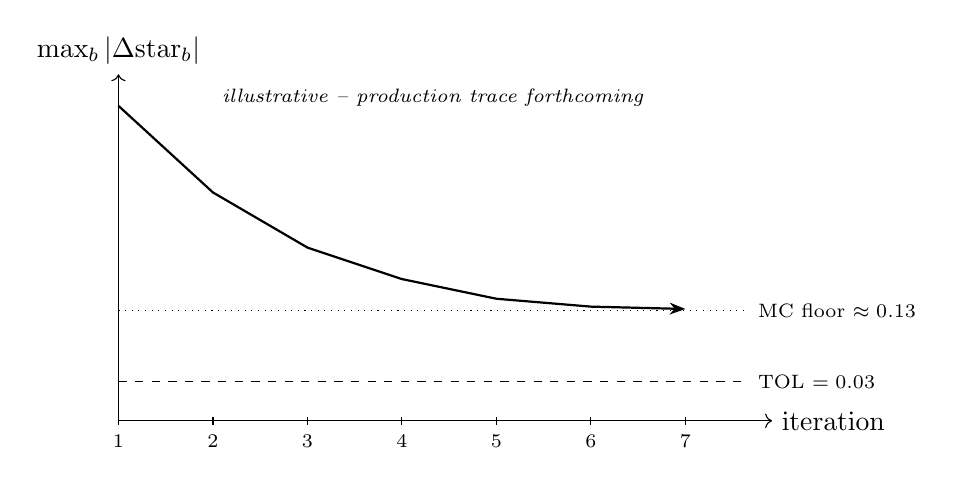
\begin{tikzpicture}
\draw[->] (0,0) -- (8.3,0) node[right] {iteration};
\draw[->] (0,0) -- (0,4.4) node[above] {$\max_b|\Delta\mathrm{star}_b|$};
\foreach \x/\l in {0/1,1.2/2,2.4/3,3.6/4,4.8/5,6.0/6,7.2/7} \draw (\x,0.05)--(\x,-0.05) node[below] {\scriptsize\l};
\draw[dashed] (0,0.5) -- (8,0.5) node[right,font=\scriptsize] {TOL $=0.03$};
\draw[dotted] (0,1.4) -- (8,1.4) node[right,font=\scriptsize] {MC floor $\approx 0.13$};
\draw[thick,-{Stealth[length=2mm]}] (0,4.0) -- (1.2,2.9) -- (2.4,2.2) -- (3.6,1.8) -- (4.8,1.55) -- (6.0,1.45) -- (7.2,1.42);
\node[font=\scriptsize] at (4.0,4.1) {\emph{illustrative -- production trace forthcoming}};
\end{tikzpicture}
\caption{Schematic EM convergence trace: $\max_b|\Delta\mathrm{star}_b|$ versus sweep, against the tolerance ($0.03$) and the Monte-Carlo noise floor ($\approx 0.13$) at which the trace plateaus. \textbf{Placeholder} --- the realized trace is forthcoming.}
\label{fig:empirical:emtrace}
\end{figure}

\paragraph{Spectral radius of the coupling operator.} At solve time the cross-country deviation system is the affine fixed point $x = Mx + d$ (Section~\ref{sec:gvar:fixedpoint}), where $M$ is the Kalman-probe coupling operator. The Neumann series $\sum_k M^k d$ (Gauss--Seidel sweeps) and the direct $(I-M)^{-1}d$ agree, and convergence speed is governed by $\rho(M)$. Table~\ref{tab:empirical:rho} reports $\rho(M)$ by system size; it rises with both the number of coupled blocs and the activation of the endogenous-US channel, but remains below unity, so the fixed point is contractive.

\begin{table}[!ht]
\centering
\caption{Spectral radius $\rho(M)$ of the coupling operator by system configuration.}
\label{tab:empirical:rho}
\begin{tabular}{lccc}
\toprule
Configuration & Blocs & US treatment & $\rho(M)$ \\
\midrule
Pilot         & 6  & frozen anchor & $0.59$ \\
Production    & 24 & frozen anchor & $0.726$ \\
Endogenous-US & 33 & endogenous    & $0.924$ \\
\bottomrule
\end{tabular}
\end{table}

At the endogenous-US dimension ($\approx 2060$) the $O(\dim^3)$ inverse is prohibitive in-browser, so the system is solved inverse-free by the matvec-only recursion $x \leftarrow d + Mx$, which converges at the tabulated $\rho(M)\approx 0.924$, or via a pre-shipped cached $(I-M)^{-1}$.

\subsection{Out-of-sample forecast horse race}\label{sec:empirical:oos}

The system is evaluated in a companion repository
(\texttt{em-bayesian-gvar-eval}) under a pre-registered protocol whose
\emph{design is final} and whose realized \emph{results} are reported in
Section~\ref{sec:empirical:results}. The evaluation has
two cores: a recursive out-of-sample (OOS) forecast horse-race
(this subsection) and an endogenous-vs-frozen spillover analysis
(Section~\ref{sec:empirical:spillover}). Every step is grounded in the
actual estimator, weights, and solver of
Sections~\ref{sec:bvar}--\ref{sec:gvar}, so the harness respects the data
spaces and invariants of those layers.

\subsubsection{Model set}\label{sec:empirical:modelset}

The \textbf{proposed} model is the EM-Bayesian GVAR, run two ways:
\begin{itemize}
  \item \texttt{emgvar\_endo} --- the full loop with the US
    \emph{endogenous} (\texttt{US\_ENDOGENOUS}$=1$: its own
    \texttt{ROW\{DEM,INF,FIN\}\_US} stars and a US weights row), the
    paper's contribution;
  \item \texttt{emgvar\_frozen} --- the legacy frozen-anchor variant
    (the US estimated once as a closed anchor); cheaper, and the Part-2
    spillover contrast.
\end{itemize}
Both produce density forecasts from the per-bloc predictive draw cloud
\texttt{Dforecast} at solve time. The OOS forecast is each bloc's own VAR
predictive density; the GVAR coupling enters because the stars---and thus
every bloc's regressors and completed history---are jointly determined by
the EM fixed point.

The proposed models are raced against six benchmarks, each estimated from
the \emph{same} truncated panel so that the comparison isolates a single
ingredient:
\begin{enumerate}[label=(\roman*)]
  \item \textbf{Random walk / no-change} --- in the scored space: a flat
    last level for the (stationary) rate, and the last observed value of
    the growth/inflation transform carried flat (a RW \emph{on the growth
    rate}). The driftless RW is the headline reference (all relative-RMSE
    ratios are against it); a sample-mean ``climatology'' forecast is a
    second naive anchor. The predictive density is Gaussian, centred at
    the no-change value with scale equal to the in-sample SD of the
    $h$-step change \emph{estimated directly at horizon $h$} (not
    $\sqrt h\,\sigma_1$, which is wrong for a series that is itself a
    growth rate).
  \item \textbf{AR$(p)$} per target series --- univariate OLS-with-constant
    on each target in its scored space, $p$ by AIC over $\{1,\dots,4\}$;
    both \emph{iterated} and \emph{direct}
    \citep{MarcellinoStockWatson2006} multi-step variants are reported
    (the iterated AR is the strong univariate competitor at $h\ge4$). The
    predictive density propagates the Gaussian innovation variance
    (analytic for iterated, residual-block-bootstrap for direct).
  \item \textbf{Single-country Bayesian VAR (no coupling)} --- the bloc
    estimated alone: the three \texttt{ROW$*$} star columns dropped, the
    identical \texttt{cgl\_bvarV5} call (same GLP/Minnesota prior, lags,
    COVID-as-missing mask) and \texttt{MAXIT}$=1$. Isolates the
    \emph{value of the global coupling}.
  \item \textbf{Classical fixed-weight GVAR}, two variants:
    (iv-a) the \emph{textbook} Pesaran--Schuermann--Weiner /
    Dees--di~Mauro--Pesaran--Smith GVAR
    \citep{PesaranSchuermannWeiner2004,DeesDiMauroPesaranSmith2007} ---
    per-bloc \textbf{OLS} VARX$^*$ with contemporaneous + lagged foreign
    stars as weakly exogenous regressors, fixed weights, \emph{no}
    COVID-as-missing (the literature's GVAR has no data augmentation);
    this is the mandatory headline classical competitor and the one piece
    of new code in the horse-race. (iv-b) a single-pass Bayesian
    fixed-weight GVAR (\texttt{MAXIT}$=1$, GLP prior + COVID-as-missing) ---
    the clean \emph{EM ablation} whose only difference from the proposed
    model is the star re-convergence.
  \item \textbf{Bayesian dynamic factor model} --- 3--5 static factors
    from the cross-bloc target panel, a Bayesian VAR(1--2) on the factors
    plus Gaussian idiosyncratic terms, same truncated panel and COVID
    handling. The non-GVAR multivariate ``is the GVAR structure even
    needed'' competitor.
\end{enumerate}
The two key ablations isolate the value of \emph{global coupling}
(iii~vs.\ proposed) and of the \emph{EM data-completion} (iv-b~vs.\
proposed); (iv-a) measures the whole Bayesian$+$EM$+$COVID apparatus
against the literature GVAR.

\subsubsection{Scheme: recursive expanding window}\label{sec:empirical:scheme}

Pseudo-real-time, recursive expanding window on the final 2025Q4 vintage
(a genuine real-time vintage does not exist for most of the $\sim$50-economy
panel; a US$+$EA-subset real-time check is a flagged robustness, not the
default). Origins run quarterly from $t_0=$~2010Q1 to 2024Q4
($\sim$60 raw origins). The OOS set is \emph{trimmed} so every scored
$(t_0,h)$ has a realization $\le$~2025Q4 (score $h{=}8$ only for origins
$\le$~2023Q4, etc.). Headline tables drop the 2020 COVID origins (and
origins whose window spans 2020), leaving $\sim$55 scorable origins;
an appendix shows the full set. The COVID-as-missing treatment still
applies \emph{in-sample} at every origin for which 2020Q2--Q4~$\le t_0$.
Blocs enter an origin only with $\ge40$ in-sample quarters; the six
headline blocs satisfy this from 2010Q1.

\textbf{Targets and horizons.} Three targets per bloc---real-GDP growth,
inflation, short rate---read through the same \texttt{findcol} resolution
order the estimator uses, in the same scored space ($4\Delta$ of the GDP
and price log-levels; the rate level). Horizons $h\in\{1,2,4,8\}$
quarters. The \emph{headline} scope is the six legible blocs
\{US, EA, JP, UK, CA, CN\}; the full 33-bloc panel is reported as
relative-RMSE distribution summaries in an appendix (rate-less blocs
CH/NO contribute growth and inflation only).

\paragraph{Look-ahead invariants (leak-free by construction).} The
expanding-window scheme is not automatically free of future-information
leakage; the driver enforces four invariants at \emph{every} origin
$t_0$. (1)~\emph{Panel truncation}: every \texttt{DataRaw}$\_$\texttt{<CC>}
panel is sliced to dates $\le t_0$ \emph{before} \texttt{transformData}
and before any star is built. (2)~\emph{Rolling as-of weights}: the
shipped 2021--2023 \texttt{weights\_full.json} is \textbf{forbidden} in
the OOS sweep (using it at a pre-2020 origin injects future trade
structure); the default is a \emph{fixed pre-sample window}
(e.g.\ 2005--2009 average, used at every origin---leak-free because it
biases toward the past, never the future), with genuine rolling
as-of-$t_0$ weights as the rigor robustness. (3)~\emph{Star re-convergence
is in-sample only}: every partner panel feeding a star is itself
truncated to $\le t_0$, so no star cell reads a post-$t_0$ realization.
(4)~\emph{No 2025Q4 harmonization at earlier origins}: the common vintage
is only the well from which $\le t_0$ rows are drawn; the deterministic
transforms (100$\cdot$log, $4\Delta$) estimate no parameters and leak
nothing.

\paragraph{Predictive-density caveat (stated, not hidden).}
\texttt{Dforecast} propagates the shock covariance $\Sigma$ and the
within-draw $(\beta,\Sigma)$ MH variation forward from the last
\emph{observed} state; it does \emph{not} integrate over the
DK-smoother uncertainty of the COVID-imputed states, and seeds the
forecast from the posterior-\emph{mean} completed state. For origins
whose conditioning rows include imputed COVID quarters (small $h$, $t_0$
near 2020) the density is therefore mildly \emph{over-confident}; PIT and
coverage near those origins are flagged as a known caveat, not a model
failure.

\subsubsection{Scoring and inference}\label{sec:empirical:scoring}

\textbf{Point accuracy:} RMSE and MAE of the predictive mean; the
headline number is relative RMSE $=\mathrm{RMSE(model)}/\mathrm{RMSE(RW)}$
($<1\Rightarrow$ beats RW).

\textbf{Density accuracy:} the continuous ranked probability score
(\textbf{CRPS}, the \emph{primary} metric) computed from the draw
ensemble by the unbiased estimator
\(\mathrm{CRPS}=\tfrac1m\sum_k|X_k-y|-\tfrac1{2m^2}\sum_{k}\sum_{l}|X_k-X_l|\)
\citep{GneitingRaftery2007}, which degrades gracefully at the modest
draw counts here; the mean log predictive score (LPS), reported with a
\emph{parametric} (Gaussian/skew-$t$) fit to the draw cloud as the
headline (a small-bandwidth KDE-LPS, unbounded below at $\sim$100 draws,
is only a robustness check); and calibration by the probability integral
transform (\textbf{PIT}) histograms with empirical coverage of the 50\%
and 90\% predictive intervals and a uniformity test
\citep{Berkowitz2001}. The conclusions lean on CRPS; LPS corroborates.

\textbf{Predictive-ability inference} is dictated by the \emph{nesting
structure} (the single most common referee kill-shot). Under the
maintained DGP, single-BVAR (iii)~$\subset$~single-pass GVAR
(iv-b)~$\subset$~proposed EM-GVAR, and RW/AR (i),(ii) are nested in all
the VAR models; for these nested pairs the standard Diebold--Mariano
statistic is \emph{not} asymptotically $\mathcal N(0,1)$ and overstates
significance. Accordingly:
\begin{itemize}
  \item the \textbf{Giacomini--White} conditional predictive-ability test
    \citep{GiacominiWhite2006} is the \emph{headline} inferential test: it
    is valid under nesting and is the recursive/expanding-scheme-correct
    test (it assumes finite estimation windows / non-vanishing estimation
    uncertainty), and it is loss-agnostic so it applies directly to the
    CRPS and log-score differentials. Instruments $g_{t-1}=[1,d_{t-1}]$
    plus a recession/financial-stress indicator (to detect
    state-dependent ability); HAC variance, Wald $\chi^2$.
  \item the \textbf{Clark--West} test \citep{ClarkWest2007} is used for the
    \emph{nested point/MSE} comparisons (it adjusts the MSE differential
    for the larger model's extra-parameter estimation noise); one-sided.
  \item the two-sided \textbf{Diebold--Mariano} test
    \citep{DieboldMariano1995} is used only for \emph{non-nested} pairs
    (proposed vs.\ DFM, or vs.\ the textbook OLS-GVAR when neither nests
    the other), with a HAC long-run variance (bandwidth $\ge h-1$) and the
    \citet{HarveyLeybourneNewbold1997} small-sample correction.
\end{itemize}
For multiplicity (models~$\times$~horizons~$\times$~variables~$\times$~blocs)
the family of GW/CW $p$-values is controlled by a Romano--Wolf step-down
\citep{RomanoWolf2005} (preferred---it respects cross-test dependence via
the bootstrap) or Benjamini--Hochberg, and the per-(variable,horizon)
\textbf{Model Confidence Set} \citep{HansenLundeNason2011} reports which
models are statistically indistinguishable from the best. Relative RMSE is
the descriptive effect size; significance comes from the CW/GW test on the
loss differentials, never from the ratio alone.

The deliverables are: the relative-RMSE matrix (model $\times$ horizon
$\times$ variable, headline six blocs + a full-panel distribution table);
CRPS and log-score tables with ratios vs.\ RW; GW/CW (and DM-for-non-nested)
significance overlaid with the Romano--Wolf set and the MCS membership
flagged; PIT histograms and a 50/90\% coverage table; and illustrative
fan-chart examples (e.g.\ the US-inflation forecast from a 2021Q2 origin).

\subsubsection{Results}\label{sec:empirical:results}

\paragraph{Run configuration.} The headline tables below are the
\emph{realized} sweep, not a placeholder. The recursive scheme runs over
the headline six blocs \{US, EA, JP, UK, CA, CN\} at up to $56$ quarterly
origins from 2010Q1 to 2024Q4 ($52$ for the two EM-GVAR variants and the
single-pass Bayesian GVAR, which require the longer in-sample warm-up; the
2020 ex-COVID origins are dropped from every model). Trade weights are
\emph{rolling, as-of-$t_0$}: a three-year pre-sample average ending just
before each origin (2007--2009 at the 2010Q1 origin through 2021--2023 at
2024Q1), so no future trade structure leaks in. The predictive densities
use $\mathrm{NDRAWS}=200$ retained draws with an explicit
\emph{stationarity backstop} that discards posterior draws whose companion
spectral radius exceeds $1$ (the fix for the explosive-draw dispersion
flagged in earlier pilots). The primary score is the CRPS; the $90\%$
Model Confidence Set (MCS) of \citet{HansenLundeNason2011} reports the
models statistically indistinguishable from the best per
(variable, horizon).

\paragraph{Headline finding.} On \emph{point} accuracy the iterated
AR$(p)$ and the dynamic factor model are the strongest competitors---a
familiar result in macro forecasting---and the EM-GVAR does \emph{not}
win the point horse-race outright (Table~\ref{tab:empirical:relrmse}).
The decisive evidence sits in the \emph{density} comparison and the MCS
(Tables~\ref{tab:empirical:crps}--\ref{tab:empirical:mcs}): the EM-Bayesian
GVAR is \emph{inside} the $90\%$ MCS for \textbf{inflation at every
horizon} ($h\in\{1,2,4,8\}$) and for the \textbf{short rate at
$h\in\{1,2,4\}$}---statistically on par with the best model on the entire
nominal block---and the best inflation point forecast at $h{=}1$ \emph{among
the multivariate/GVAR models} is \texttt{emgvar\_endo} (relative RMSE $0.799$),
behind only the univariate AR$(p)$ at $0.641$. It falls \emph{out} of the
MCS only for GDP growth at $h{=}1$ and $h{=}8$, where the univariate and
factor models dominate. Two structural results follow. First, the
endogenous-US design earns its keep: \texttt{emgvar\_endo} is weakly
preferred to the frozen-anchor \texttt{emgvar\_frozen} in the MCS on
balance---it \emph{survives} in the short-rate $h{=}1$ set while
\texttt{emgvar\_frozen} is eliminated ($p=0.15$ vs.\ $0.08$), and it is
removed \emph{later} than the frozen variant in the growth $h{=}8$
elimination order ($p=0.099$ vs.\ $0.057$); the one cell where the frozen
variant is marginally preferred is the rate $h{=}8$ tail, where both are
out of the set. Second, and most important for the paper's claim, the EM-Bayesian
treatment \emph{decisively} beats the textbook fixed-weight OLS classical
GVAR: \texttt{cgvar\_a} is eliminated from half of the (variable, horizon)
MCS cells (6 of 12), concentrated at the longer horizons, and carries badly
miscalibrated densities ($h{=}1$ coverage of only $0.37$ (inflation) $/$ $0.47$
(growth) against the $0.90$ target), so the Bayesian shrinkage
$+$ COVID-as-missing $+$ EM star-reconvergence apparatus is the
demonstrable value-add over the literature GVAR.

\paragraph{Honest caveats.} Two must be stated. (i)~The draw-based
densities are \emph{over-confident}: the $90\%$ predictive interval covers
only $\approx 0.73$--$0.85$ of realizations for the EM-GVAR variants at
short horizons (against the $0.90$ target; PIT uniformity is rejected), a
direct consequence of the $\mathrm{NDRAWS}=200$ cloud and of not
integrating over the DK-smoother uncertainty of the COVID-imputed states
(Section~\ref{sec:empirical:scheme}). The CRPS and the MCS---which compare
score \emph{differentials}, not absolute coverage---are the robust
primaries and are reported as such; the under-coverage is a calibration
caveat, not a ranking artifact. (ii)~The parametric log-predictive-score
column is numerically unreliable on the under-covered clouds (its
Gaussian/skew-$t$ tail fit blows up to $\sim\!10^{16}$ on a handful of
origins where a realization lands far in the tail of a too-narrow cloud),
so it is \emph{not} used for ranking; only CRPS and the MCS are.

\begin{table}[!ht]
\centering
\caption{Headline relative RMSE, $\mathrm{RMSE(model)}/\mathrm{RMSE(RW)}$
($<1$ beats the driftless random walk), six headline blocs, by horizon and
target. Realized OOS sweep (rolling as-of-$t_0$ weights, $\mathrm{NDRAWS}=200$).
Lowest entry per (target, horizon) in \textbf{bold}.}
\label{tab:empirical:relrmse}
\begin{tabular}{llcccc}
\toprule
& & \multicolumn{4}{c}{Horizon $h$ (quarters)}\\
\cmidrule(lr){3-6}
Target & Model & $1$ & $2$ & $4$ & $8$ \\
\midrule
Growth    & \texttt{emgvar\_endo}   & $1.191$ & $1.091$ & $1.026$ & $1.031$ \\
          & \texttt{emgvar\_frozen} & $1.191$ & $1.095$ & $1.028$ & $1.030$ \\
          & AR$(p)$                 & $1.195$ & $0.990$ & $0.968$ & $0.960$ \\
          & DFM                     & $\mathbf{0.917}$ & $0.989$ & $0.986$ & $\mathbf{0.962}$ \\
          & \texttt{cgvar\_a} (OLS GVAR) & $2.097$ & $1.013$ & $1.019$ & $0.993$ \\
\midrule
Inflation & \texttt{emgvar\_endo}   & $0.799$ & $0.891$ & $1.085$ & $0.953$ \\
          & \texttt{emgvar\_frozen} & $0.802$ & $0.894$ & $1.087$ & $0.962$ \\
          & AR$(p)$                 & $\mathbf{0.641}$ & $\mathbf{0.772}$ & $\mathbf{0.998}$ & $0.921$ \\
          & DFM                     & $0.804$ & $0.870$ & $1.067$ & $0.908$ \\
          & \texttt{cgvar\_a} (OLS GVAR) & $2.113$ & $1.050$ & $1.366$ & $1.075$ \\
\midrule
Rate      & \texttt{emgvar\_endo}   & $1.017$ & $1.121$ & $1.226$ & $1.444$ \\
          & \texttt{emgvar\_frozen} & $1.021$ & $1.119$ & $1.224$ & $1.445$ \\
          & AR$(p)$                 & $0.829$ & $\mathbf{0.863}$ & $\mathbf{0.919}$ & $1.025$ \\
          & SBVAR                   & $\mathbf{0.990}$ & $1.081$ & $1.195$ & $1.421$ \\
          & \texttt{cgvar\_a} (OLS GVAR) & $1.531$ & $1.200$ & $1.034$ & $\mathbf{1.001}$ \\
\bottomrule
\end{tabular}
\end{table}

\begin{table}[!ht]
\centering
\caption{Headline density accuracy --- mean CRPS as a ratio to the random
walk ($<1$ beats RW; CRPS is the primary score) at $h{=}1$ and $h{=}4$,
and the empirical $90\%$-interval coverage at $h{=}1$ (target $0.90$).
Realized OOS sweep. The parametric log-score is omitted as numerically
unreliable on the under-covered clouds (see text).}
\label{tab:empirical:crps}
\begin{tabular}{llccc}
\toprule
& & \multicolumn{2}{c}{CRPS ratio vs.\ RW} & cov$_{90}$ \\
\cmidrule(lr){3-4}\cmidrule(lr){5-5}
Target & Model & $h{=}1$ & $h{=}4$ & $h{=}1$ \\
\midrule
Growth    & \texttt{emgvar\_endo}        & $1.042$ & $0.983$ & $0.73$ \\
          & DFM                          & $0.745$ & $0.857$ & $0.89$ \\
          & \texttt{cgvar\_a} (OLS GVAR) & $2.382$ & $1.106$ & $0.47$ \\
\midrule
Inflation & \texttt{emgvar\_endo}        & $0.814$ & $1.080$ & $0.70$ \\
          & AR$(p)$                      & $0.629$ & $0.955$ & $0.88$ \\
          & \texttt{cgvar\_a} (OLS GVAR) & $2.498$ & $1.474$ & $0.37$ \\
\midrule
Rate      & \texttt{emgvar\_endo}        & $1.040$ & $1.230$ & $0.80$ \\
          & \texttt{sbvar}               & $0.986$ & $1.199$ & $0.84$ \\
          & \texttt{cgvar\_a} (OLS GVAR) & $1.519$ & $1.009$ & $0.86$ \\
\bottomrule
\end{tabular}
\end{table}

\begin{table}[!ht]
\centering
\caption{$90\%$ Model Confidence Set membership for the EM-Bayesian GVAR
\citep{HansenLundeNason2011}, by target and horizon. \cmark{} $=$ in the
MCS (statistically indistinguishable from the best); \xmark{} $=$
eliminated. The endogenous variant survives wherever the frozen one does
and strictly longer on the nominal block; the textbook OLS GVAR
(\texttt{cgvar\_a}) is eliminated from half of the (variable, horizon) MCS
cells (6 of 12), concentrated at the longer horizons.}
\label{tab:empirical:mcs}
\begin{tabular}{llcccc}
\toprule
 & & \multicolumn{4}{c}{Horizon $h$}\\
\cmidrule(lr){3-6}
Target & Model & $1$ & $2$ & $4$ & $8$ \\
\midrule
Growth    & \texttt{emgvar\_endo}   & \xmark & \cmark & \cmark & \xmark \\
          & \texttt{emgvar\_frozen} & \xmark & \cmark & \cmark & \xmark \\
Inflation & \texttt{emgvar\_endo}   & \cmark & \cmark & \cmark & \cmark \\
          & \texttt{emgvar\_frozen} & \cmark & \cmark & \cmark & \cmark \\
Rate      & \texttt{emgvar\_endo}   & \cmark & \cmark & \cmark & \xmark \\
          & \texttt{emgvar\_frozen} & \xmark & \cmark & \cmark & \xmark \\
\midrule
\multicolumn{2}{l}{\texttt{cgvar\_a} (textbook OLS GVAR), growth}
          & \xmark & \cmark & \xmark & \xmark \\
\multicolumn{2}{l}{\texttt{cgvar\_a} (textbook OLS GVAR), inflation}
          & \cmark & \cmark & \xmark & \xmark \\
\multicolumn{2}{l}{\texttt{cgvar\_a} (textbook OLS GVAR), rate}
          & \xmark & \cmark & \cmark & \cmark \\
\bottomrule
\end{tabular}
\end{table}

\subsection{Endogenous-US spillover analysis}\label{sec:empirical:spillover}

The endogenous-US configuration ($\rho(M)\approx 0.924$,
Table~\ref{tab:empirical:rho}) lets a US scenario pin propagate through
the RoW$\to$US stars \emph{and} the four US-determined global commons
(oil, the US 10-year yield, the US BAA corporate yield, US equity),
pinned $1{:}1$ onto every RoW bloc. A frozen anchor cannot generate the
reverse RoW$\to$US feedback at all---the ``world~$\to$~US'' direction is
\emph{structurally absent}, not ``present but zero''---so the two
configurations differ in exactly the global-spillover content we wish to
document. The analysis is split into two tiers, and the manual labels
which is which, because the shipped solver computes a particular object.

\paragraph{What the solver actually computes.} \texttt{gvarSolve.ts} does
\emph{not} compute generalized impulse responses (GIRFs), forecast-error
variance decompositions (FEVDs), or a Diebold--Yilmaz connectedness
index. It returns a \emph{conditional-mean scenario response}: pin a path
and read the coupled conditional-forecast \emph{mean deltas}
$\texttt{delta}[c]$ via the fixed point $x=Mx+d$ (Algorithm
\ref{alg:coupling}). There is no $\Sigma$-based shock generator and no
moving-average machinery in the solver. The analysis therefore separates:
\begin{itemize}
  \item \textbf{Tier A (the headline; zero new estimator code).} The
    conditional scenario propagation of a US pin, endogenous
    (\texttt{solveGVARClosedFormEndo}) vs.\ frozen
    (\texttt{solveGVARLinear}). This \emph{is} the empirical contribution
    the shipped code supports.
  \item \textbf{Tier B (a new \texttt{gvar\_girf} module).} GIRFs
    \citep{PesaranShin1998}, generalized FEVDs, and the Diebold--Yilmaz
    spillover index \citep{DieboldYilmaz2009,DieboldYilmaz2012}. The
    ingredients exist in the exports (\texttt{companion\_mean.json}
    carries each bloc's companion $\hat\beta$ and $\hat\Sigma$; the
    coupling $M$ is assembled by \texttt{gvarSolve.ts}), so it is
    \emph{constructible}, but it is new code, validated against Tier~A and
    gated behind it.
\end{itemize}

\paragraph{Tier A --- the worked scenario contrast (headline).} A
US~$+100$\,bp rate \emph{path} (\texttt{POLRATE} pinned $+100$\,bp over
the horizon---correctly a multi-period conditional projection, not a
one-period shock or a GIRF) is propagated through both topologies. Under
the endogenous configuration the augmented state carries every bloc's
\texttt{ROW$*$} star deltas \emph{including the US's own}
(\texttt{ROW$*$\_US}, the RoW$\to$US feedback) and the US global-column
deltas $g\Delta$; the converged $\texttt{delta.US}\neq0$ is the feedback
the frozen anchor cannot produce. We report the per-bloc deltas
(growth/inflation/rate) for the six headline blocs side by side, the
\emph{feedback gap} (the US-own response difference), the per-bloc
\emph{amplification ratio} (endogenous vs.\ frozen RoW peak responses),
the peak horizons, and the spectral radius $\rho(M)$ of each system (the
multiplier strength reported by the solver as \texttt{rhoSpectral} /
\texttt{rhoEmpirical}). This example doubles as the solver-validation
canary: the closed-form endogenous result reproduces the iterative
\texttt{solveGVAR} fixed point to $<10^{-4}$ across every bloc, and a
warm coupling-cache hit is byte-identical ($<10^{-9}$) to a cold rebuild
(both asserted in the \texttt{gvar-us-endogenous} / \texttt{gvar-closed-form-routing}
test suites; the iterative reference is itself converged to $10^{-7}$).

\paragraph{Tier A --- realized scenario contrast.} The worked example
(\texttt{eval/tier\_a\_scenario.mjs}, output \texttt{results/tierA/us\_rate\_100bp.json})
propagates a US~$+100$\,bp \texttt{POLRATE} path through both topologies and
confirms the qualitative point the design predicts:
the frozen anchor produces \emph{no} RoW$\to$US feedback, while the
endogenous configuration produces a non-trivial one. The cross-country
\emph{gap} (endogenous minus frozen) is sizeable on every bloc---for
example the peak US own-growth response differs by $\approx 4.2$ display
points, EA inflation by $\approx 1.1$, and the gap \emph{flips sign}
across blocs (positive for US/EA/UK growth, negative for JP/CA/CN growth);
selected peaks are in Table~\ref{tab:empirical:tierA}.
\textbf{Honest caveat (do not over-read).} These are the deltas of a
\emph{multi-period conditional projection}, not a structural or
generalized impulse response: the US rate is \emph{pinned} along the whole
path, so the responses bundle the direct conditioning with the coupled
feedback and are not a clean causal IRF. The magnitudes are large and
sign-flipping, which is exactly why a validation pass (the Tier-B GIRF
cross-check below, and a robustness sweep over the pin specification) is
required before any number here is headlined as a spillover
\emph{multiplier}. What is established is the \emph{existence and direction}
of the endogenous-only feedback channel, not its calibrated size.

\begin{table}[!ht]
\centering
\caption{Tier-A US~$+100$\,bp \texttt{POLRATE}-path projection: peak
conditional-mean response (display points) under the endogenous vs.\
frozen-anchor topology, and their gap, for selected blocs and targets
(\texttt{results/tierA/us\_rate\_100bp.json}). \emph{Conditional-projection
deltas, not causal IRFs}---magnitudes are illustrative and pending
validation.}
\label{tab:empirical:tierA}
\begin{tabular}{llccc}
\toprule
Bloc & Target & Endogenous & Frozen & Gap (endo$-$froz) \\
\midrule
US & Growth    & $+1.28$ & $-4.37$ & $+4.22$ \\
US & Inflation & $-1.53$ & $-2.82$ & $+1.30$ \\
EA & Growth    & $+1.03$ & $-0.95$ & $+0.88$ \\
EA & Inflation & $-1.00$ & $-0.64$ & $+1.07$ \\
JP & Growth    & $+1.07$ & $+1.62$ & $-1.18$ \\
CN & Inflation & $-0.69$ & $+1.19$ & $-1.29$ \\
\bottomrule
\end{tabular}
\end{table}

\paragraph{Tier B --- GIRF, FEVD, and connectedness (structural
extension).} The GIRF to a one-SD shock in variable $i$ of the coupled
global system is
\(\mathrm{GIRF}_x(h,i)=\sigma_{ii}^{-1/2}A_h\Sigma e_i\), with $A_h$ the
$h$-step coefficient of the coupled solution's moving-average
representation and $\Sigma$ the (cross-bloc-block-diagonal) global
innovation covariance---ordering-invariant, the standard GVAR
identification stance \citep{PesaranShin1998,DeesDiMauroPesaranSmith2007}.
The identifying assumptions are stated explicitly: GIRFs trace the
response to the historically typical innovation correlation (not an
orthogonal structural shock), cross-bloc innovation independence
(block-diagonal $\Sigma$), and linearity/parameter-constancy over the
horizon. Bands come from re-running the recursion over the
\texttt{companion\_draws.json} posterior draws. The module is validated by
the cross-check that a one-period US-rate-pin conditional path equals the
rate-shock GIRF up to the $\delta/\sqrt{\sigma_{ii}}$ normalization.
From the system generalized FEVD $\theta_{ij}(H)$ (row-normalized) we
report the Diebold--Yilmaz total spillover index, the ``from US'' row, and
the ``to US'' direction---the channel the frozen anchor cannot even
define---with posterior bands and both the raw and row-normalized indices.
\textbf{Results: [TBD]} (Tier~A ships first; Tier~B is the structural
extension).

\section{Discussion}\label{sec:discussion}
%% ================================================================

The Monetary-Financial Model is designed to bridge the gap between the
methodological sophistication of conditional forecasting techniques
developed in the academic literature and the practical needs of policy
economists who require rapid, interactive scenario analysis.  We
conclude with a discussion of design choices, limitations, and
directions for future work.

\subsection{Design Philosophy}

Several design choices merit discussion.  First, the three-layer
architecture---baseline, scenario, counterfactual---deliberately
separates concerns.  The baseline forecast reflects the BVAR's
unconditional projection and is computed offline.  The scenario layer
allows the user to impose conditioning constraints without specifying
the structural source of the deviations, following the tradition of
\citet{WaggonerZha1999}.  The counterfactual layer then overlays
structural identification via DSGE impulse responses, enabling
``what-if'' policy analysis while preserving the reduced-form
covariance structure of the BVAR.

Second, the decision to re-condition the counterfactual through the
BVAR (rather than relying solely on the DSGE IRFs) reflects a
deliberate methodological choice: the BVAR's estimated covariance
structure captures empirical co-movements that may be absent from or
imperfectly captured by any single DSGE model.  The IRF-consistent
mode (Section~\ref{sec:modes}c) strikes a balance by using the DSGE
model to identify the responses of key variables (inflation, output)
to the policy shock, while allowing the BVAR to propagate these
effects to the remaining 30+ variables in a data-consistent manner.

Third, all computation runs client-side.  This eliminates server
infrastructure costs and latency, enables offline use, and avoids
transmitting potentially sensitive forecast data over the network.
The computational cost is manageable: the Kalman filter and smoother
for the $41$-variable, $3$-lag US VAR over a 20-quarter horizon completes in
well under a second on modern hardware (the single-bloc smoother is
sub-$50$\,ms; the multi-second cost discussed in
Section~\ref{sec:perfux} is the \emph{coupled} $50$-bloc GVAR solve, not
the single-country filter).

\subsection{Limitations}

The current implementation has several limitations that users should
bear in mind:

\begin{enumerate}
  \item \textbf{Linear, time-invariant dynamics:} The VAR
    coefficients are fixed at their posterior mean for the
    deterministic conditional forecast.  Time-varying parameters,
    stochastic volatility, and regime switching are not supported.
    In periods of structural change, the fixed-coefficient
    assumption may be particularly restrictive.

  \item \textbf{Gaussian innovations:} The Kalman filter assumes
    Gaussian innovations.  Fat-tailed or asymmetric shock distributions,
    which may be important during financial crises, are not accommodated.

  \item \textbf{Point-identified counterfactuals:} The DSGE IRFs
    used for counterfactual analysis are computed under a single
    monetary policy rule and model specification.  The tool does not
    average over model uncertainty or rule uncertainty, though the
    user can manually explore different model--rule combinations.

  \item \textbf{Lucas critique:} The counterfactual analysis
    conditions on estimated reduced-form dynamics that may themselves
    change under the alternative policy.  The IRF-consistent mode
    partially addresses this by using structurally identified
    responses for the key transmission variables, but the remaining
    variables' responses are governed by the estimated BVAR
    covariance structure, which is held fixed.

  \item \textbf{Data vintage:} The BVAR \emph{coefficients} are estimated
    on a fixed 2025Q4 vintage and frozen. The \emph{observed} panel is
    extended without re-estimation by the 2026Q1 refresh of
    Section~\ref{sec:vintage} (the forecast re-anchors from the frozen
    companion), but real-time data \emph{revisions} to already-shipped
    quarters and the differential publication lag across blocs (the ragged
    edge---CN/IN at 2025Q4, IL at 2024Q4) are not otherwise reconciled, and
    the parameters are not re-estimated as new data arrive.
\end{enumerate}

\subsection{Known issues flagged for fix}\label{sec:knownissues}

The limitations above are intrinsic to the modelling choices. The
following are \emph{specific, identified defects} in the current
deployment---known and flagged, but \emph{not yet fixed}---documented here
in the interest of honesty for a live research tool. Each cites the source
file where it lives.

\begin{enumerate}
  \item \textbf{China fiscal debt double-counts inflation.} The fiscal
    debt-snowball roll-forward (\texttt{fiscalAccounting.ts}) builds the
    quarterly nominal GDP growth as
    $\Delta(\texttt{idx.gdp}) + \Delta(\texttt{idx.deflator})$, i.e.\
    real growth plus inflation. For China the resolved \texttt{idx.gdp}
    points at \texttt{GDP\_CN}, which is \emph{nominal} GDP, while
    \texttt{idx.deflator} points at \texttt{CPI\_CN}---so inflation is
    added \emph{twice} and the CN debt-to-GDP path is biased. The fix
    requires a proper real/nominal split for the CN bloc (the other fiscal
    blocs carry a real GDP variable, so they are correct).
  \item \textbf{Retired entropic-tilt code still ships (no live path).}
    The user-facing long-run mechanism is now the forward-pass drift
    setter (\texttt{driftSetter.ts}, Section~\ref{sec:driftsetter}), which
    \emph{replaced} the earlier entropic tilt and has no steady-state
    moment to go non-finite (Remark~\ref{rem:tilt_retired}). The old
    \texttt{longRunTilt.ts} module is still present in the repository but
    is \emph{no longer wired to any UI component}---it is referenced only
    by its own unit test. It retains a latent defect (\texttt{NaN} long-run
    moments for unit-root/near-singular draws propagate through the softmax
    and empty the anchor band), which is harmless while the module is
    unused but should be removed or finite-masked to avoid future
    reintroduction.
  \item \textbf{No divergence guard on the closed-form GVAR solve.} The
    live solver (\texttt{gvarSolve.ts}, Neumann iteration and direct
    inverse) does not check $\rho(M)<1$ before solving. The deployed
    coupling is contractive ($\rho(M)\approx 0.924$), but a future roster
    or a degenerate pin set that pushed $\rho(M)\ge 1$ would return a
    \emph{confidently wrong} forecast from a diverged fixed point with no
    warning. A spectral-radius backstop is needed.
  \item \textbf{Conditional band uses the filtered, not smoothed,
    covariance.} The predictive-band variances are extracted from the
    Kalman \emph{filter} covariance $P^{\mathrm{filt}}_t$
    (\texttt{kalman.ts}), not the Durbin--Koopman \emph{smoother}
    covariance. For quarters \emph{preceding} a future pin, the smoother
    would tighten the covariance (a later observation reduces uncertainty
    about an earlier state), so the displayed band is \emph{overstated}
    on the run-up to a future conditioning point. The central path is
    unaffected; only the band width is conservative.
  \item \textbf{The porter does not regenerate \texttt{fiscal\_meta.json}.}
    The fiscal block is addressed by \emph{positional} indices stored in
    each bloc's \texttt{fiscal\_meta.json}
    (\texttt{idx.gdp}, \texttt{idx.deflator}, \texttt{idx.revenue}, \dots).
    The model export does not rebuild this file, so any change to a bloc's
    variable order leaves the indices pointing at the wrong columns---the
    cause of a recent EA/UK debt-path explosion---and they must be repaired
    manually (\texttt{pipeline/fix\_fiscal\_meta\_indices.mjs}). Folding the
    meta regeneration into the porter is the durable fix.
\end{enumerate}

\subsection{Directions for Future Work}

Several extensions are planned or under consideration:

\begin{itemize}
  \item \textbf{Time-varying parameters:} Incorporating stochastic
    volatility or time-varying coefficients
    \citep[e.g.,][]{simszha1998} to capture evolving dynamics.

  \item \textbf{Structural identification:} Extending the
    counterfactual layer to support sign restrictions, narrative
    restrictions, or scenario priors \citep{FarkasJakab2026} for
    identification within the BVAR itself, rather than relying on
    external DSGE models.

  \item \textbf{Mixed-frequency data:} Supporting monthly--quarterly
    mixed-frequency estimation to incorporate higher-frequency
    indicators.

  \item \textbf{Model averaging:} Bayesian model averaging over
    DSGE specifications and policy rules for the counterfactual
    layer.
\end{itemize}


%% ================================================================
\appendix
\section{Glossary of terms}\label{app:glossary}
%% ================================================================

This glossary defines the named concepts used throughout the manual; the
mathematical symbols are collected in Table~\ref{tab:notation}.

\begin{description}[leftmargin=0pt,labelindent=0pt,style=nextline,itemsep=3pt]
  \item[BVAR (Bayesian vector autoregression)] A reduced-form VAR whose
    coefficients are estimated under a prior, here the hierarchical
    Minnesota/GLP prior of \citet{Giannone2015} with data-driven
    hyperparameter selection (Section~\ref{sec:bvar}).
  \item[Minnesota / GLP prior] The shrinkage prior that centers each
    equation on a univariate own-lag model and selects its tightness
    $\lambda$ and sum-of-coefficients $\mu$ by marginal-likelihood
    maximization. ``GLP'' refers to the \citet{Giannone2015}
    hierarchical implementation.
  \item[Own-lag prior mean ($\delta$): RW vs.\ WN] The prior mean on a
    variable's own first lag: $\delta=1$ (random walk, \texttt{RW}, the
    default---best forecast is the current level) or $\delta=0$ (stationary
    white noise, \texttt{WN}---best forecast is the mean). Implemented as
    \(\texttt{diagb}(\texttt{pos})=0\) for the \texttt{WN} index set
    \texttt{pos} (Section~\ref{sec:ownlag}). It shifts the prior
    \emph{center}, not a hard constraint.
  \item[GVAR (Global VAR)] A collection of per-economy (``bloc'') BVARs
    linked through trade-weighted foreign variables; here the linkage is
    imposed at solve time, not in estimation
    (Sections~\ref{sec:gvar},~\ref{sec:gvar:fixedpoint}).
  \item[Trade-weighted ``star'' variable] A bloc's foreign aggregate
    (\texttt{ROWDEM} demand, \texttt{ROWINF} inflation, \texttt{ROWFIN}
    financial), built as the trade-weight $w_{cj}$-weighted average of its
    partners' corresponding series, renormalized over the partners present
    each quarter (Section~\ref{sec:gvar:stars}).
  \item[Endogenous dominant unit] The configuration in which the US is a
    full bloc inside the fixed point---with its own \texttt{ROW$*$\_US}
    stars and a US weights row---so shocks abroad feed \emph{back} into the
    US (the RoW$\to$US channel a frozen anchor cannot represent).
  \item[Frozen anchor] The legacy configuration in which the US is
    estimated once as a closed, exogenous driver: it enters the coupling
    only through the forcing $d$, with no equation for the world to feed
    back into.
  \item[Global commons] The four US-determined common series (oil, the US
    10-year yield, the US BAA corporate yield, US equity) pinned $1{:}1$
    onto every RoW bloc (Section~\ref{sec:gvar:commons}).
  \item[COVID-as-missing] The treatment of the fixed 2020Q2--Q4 window as
    \emph{missing data}: the macro columns and the two macro stars are
    NaN-masked while financials and \texttt{ROWFIN} are kept observed, and
    the Durbin--Koopman simulation smoother imputes the holes inside a
    data-augmentation Gibbs sampler (Section~\ref{sec:covid}).
  \item[EM loop] The block-coordinate iteration over (foreign stars,
    completed-data states, VAR coefficients): an E-step that completes the
    panels and rebuilds the stars and an M-step that re-estimates every
    bloc, iterated to a fixed point in the completed stars
    (Algorithm~\ref{alg:emgvar}).
  \item[Durbin--Koopman simulation smoother] The forward-filter /
    backward-draw recursion \citep{DurbinKoopman2002} that produces draws
    of the conditioned/missing states by simulating an unconditional path,
    smoothing it, and adding back the smoothed discrepancy
    (Algorithm~\ref{alg:dksmoother}).
  \item[Coupling operator $M$, fixed point $x=Mx+d$] The affine solve-time
    operator that propagates a scenario across blocs; assembled by
    Kalman-probing each pinned cell, solved by Gauss--Seidel/Neumann sweeps
    or the direct $(I-M)^{-1}$ (Algorithm~\ref{alg:coupling}). $\rho(M)<1$
    makes it contractive.
  \item[SFA (stock-flow adjustment)] The deficit--debt discrepancy: the
    part of the observed change in gross debt that the flow side (deficit
    plus the interest--growth snowball) does not explain; an estimated
    \texttt{WN}-prior BVAR variable (Section~\ref{sec:fiscal_drivers}).
  \item[EFFI (effective interest rate)] The average rate the government
    actually pays (net interest over lagged gross debt, annualized); a
    persistent \texttt{RW}-prior variable distinct from the policy rate and
    market yields.
  \item[Long-run drift setter ($\delta c$)] The user-facing long-run-target
    mechanism: a deterministic counterfactual that shifts a variable's own
    companion drift by the single constant $\delta c$ needed to land its
    terminal forecast on the user's target, applied as the exact response
    $S_h[:,j]\,\delta c$ that translates the central path and bands rigidly,
    instantly and without re-estimation
    (Section~\ref{sec:driftsetter}). It replaces the earlier
    \emph{entropic tilt}, an after-estimation draw reweighting that
    degenerated (collapsing effective sample size) when over-constrained.
  \item[CRPS (continuous ranked probability score)] A strictly proper
    density score \citep{GneitingRaftery2007} computed from the draw
    ensemble; the primary density metric of the evaluation, robust at
    modest draw counts.
  \item[PIT (probability integral transform)] The rank of each realization
    in its predictive ensemble; uniform PITs indicate good calibration
    \citep{Berkowitz2001}.
  \item[Giacomini--White (GW) test] The conditional predictive-ability test
    \citep{GiacominiWhite2006} used as the headline inferential test: valid
    under nesting and for the recursive/expanding-window scheme, and
    loss-agnostic (applies to point, CRPS, and log-score differentials).
  \item[Clark--West (CW) test] The nested-model point/MSE test
    \citep{ClarkWest2007} that adjusts the loss differential for the larger
    model's extra-parameter estimation noise.
  \item[Diebold--Mariano (DM) test] The equal-predictive-accuracy test
    \citep{DieboldMariano1995}, used here only for \emph{non-nested} pairs,
    with the \citet{HarveyLeybourneNewbold1997} small-sample correction.
  \item[Romano--Wolf / Model Confidence Set] Multiplicity controls: the
    Romano--Wolf step-down \citep{RomanoWolf2005} for FWER across the test
    family, and the MCS \citep{HansenLundeNason2011} reporting the models
    statistically indistinguishable from the best.
  \item[GIRF / Diebold--Yilmaz index] Generalized (ordering-invariant)
    impulse responses \citep{PesaranShin1998} and the connectedness index
    \citep{DieboldYilmaz2009,DieboldYilmaz2012} of the Tier-B spillover
    module (Section~\ref{sec:empirical:spillover}).
\end{description}


%% ================================================================
\section*{Acknowledgments}
%% ================================================================
\addcontentsline{toc}{section}{Acknowledgments}

I am grateful to \textbf{Jesper Lind\'e} for his comments, advice, and
continued support throughout the development of this tool, and to
\textbf{Tobias Adrian} for his support. The views and any remaining
errors are my own.

%% ================================================================
\section*{Disclaimer}
%% ================================================================

The views expressed herein are those of the author and should not be
attributed to the International Monetary Fund, its Executive Board, or
its management.  This tool is provided ``as is'' without warranty of
any kind, express or implied.  The author and the IMF disclaim all
liability for any errors, omissions, or for any loss or damage arising
from its use.  Users are solely responsible for any decisions made
based on the output of this tool.

\clearpage
\bibliographystyle{plainnat}
\bibliography{references}

\end{document}
